\chapter{Evaluation}
\label{chapter:evaluation}

In this chapter, we evaluate our WebAssembly executor by comparing it to OpenWhisk vanilla. First we discuss and define the types of workloads we use in our experiments. Then we go into details of our methodology, the experimental setup, which metrics we measure and what hardware we deploy on. All that will lead to answers for our research questions.

\section{Methodology}

\subsection{Goals}

Recall our research questions.

\begin{enumerate}
    \item By how much can WebAssembly runtimes alleviate the cold start latency?
  
    \item How do the performance characteristics of the WebAssembly and Docker container runtimes differ?
  
    \item What are the resource costs for keeping containers warm in both container runtimes?
  
    \item Which WebAssembly runtime is the most suitable for use on edge devices?
\end{enumerate}

% In order to answer these questions, we need to measure 
% These questions guide our evaluation approach.

\subsection{Workload Types}

In Chapter \ref{chapter:background} we described the serverless workload in detail, which guided decisions in our implementation. Specifically, we already used that research to get an idea about what concurrency model may be a better fit for our executor.

This research workload represents the current \emph{cloud} workload and may or may not be transferable to workloads at the edge. Because of that, we also take some examples of visionary and potential use cases into account and infer scenarios, i.e. the order of cold starts and warm starts, as well as workload types, i.e. whether functions are CPU- or I/O-bound. That includes both serverless edge workloads and latency-sensitive ones.

% To measure the performance of the serverless platform in a meaningful way, we reviewed the literature for use cases, where latency is critical; in turn, where the cold start time matters most. From these examples as well as characterizations of the workload types in section \ref{section:serverless_workload}, we infer an evaluation workload.


\begin{description}[style=multiline, leftmargin=2.5cm, font=\bfseries]

    \item[Vital Signs Analysis] \citeauthor{Nastic2017} introduce measuring a patient's vital signs with wearable sensors during a situation of crisis \cite{Nastic2017}. Since lives are at stake, decisions must be made quickly. The scenario is both a latency-critical and an edge computing application. It serves as an example, where a serverless platform on edge computers can provide lower latency than sending the data to the cloud. Thus, part of the latency is reduced by moving the computation physically closer to the sensor. However, the second important factor for latency is the platform's execution time. When a sensor comes online and sends its first request, the execution suffers from a cold start. Once sensors are online, they need to analyze data in real time and continuously. Therefore, when the cold start happens, the platform may already be under load from other requests, and there may be concurrent cold starts. This is a scenario where high performance and efficient usage of the limited resources is required, and one where the same functions are called repeatedly -- warm starts.
    The workload itself is data analytics, but not described in more detail. We classify this as primarily CPU-bound, because we can assume it involves data preprocessing, statistical analysis and perhaps even machine learning inference.

    \item[Edge AI] \citeauthor{Rausch2019} describe a motivational use cases for AI at the serverless edge. A personal bio sensor measures blood sugar levels and sends it to an edge device, which refines a pre-trained model with that data and serves the model for inferencing \cite{Rausch2019}. The workload for this type of serverless function needs a significant amount of CPU-time for the machine learning tasks but also writes and reads parts of the model to and from disk. We classify this as both CPU- and file-I/O-bound. Considering that measuring blood sugar levels is sufficient in greater intervals, e.g. 10 minutes, or whenever the user does a manual measurement, each of those would spawn a function that does the analysis and training, but could be discarded once it is finished. That is, keeping the function warm would be unnecessary and wasting resources. If the user actively took the measurement and waits for the analysis results, a low latency is required for a good quality of experience. Thus, the cold start of the analysis function should be as short as possible.
    
    \item[Augmented Reality] \citeauthor{Huang2012} implemented a mobile augmented reality (AR) system that analyzes images of book spines locally, e.g. on a smartphone, and then sends the features to the cloud to find a match in a database \cite{Huang2012}. \citeauthor{Baresi2019} propose to offload the image recognition task to a more powerful edge device, to save on battery on the hosting device \cite{Baresi2019}. AR applications require a low latency to provide a good user experience. Offloading such recognition tasks to nearby and more powerful edge devices presupposes their capability to execute them at high speed. This is a scenario where a serverless platform would receive a high number of concurrent CPU-bound requests.

    \item[APIs] According to \citeauthor{Eismann2021a} -- who conducted a manual analysis of serverless applications -- 28\% of their analyzed applications were APIs \cite{Eismann2021a}. Even with today's cold start latency, developers are already using serverless for user-facing applications, where latency is rather important. However, as \citeauthor{Leitner2019} noted in their interviews with practitioners, many of them voiced concerns about the high latency associated with cold starts \cite{Leitner2019}. If the latency could be reduced significantly, even the APIs of latency-sensitive applications can be built on serverless. A useful API is typically accessing or modifying state. Since serverless functions by themselves are stateless, they need to communicate with other services such as databases, event buses and logging services. This composition requires many network I/O-bound calls and is usually light on the CPU, since the function spends most of its time waiting for I/O to complete.

\end{description}

We infer two workloads from these, while also taking into account our previous research. Both CPU- and network I/O-bound workloads are a primary type that ought to be handled well by a serverless platform. Some limitations apply due to WASI's immaturity or serverless idiosyncrasies. In particular, to model a full machine learning example, we should access an already trained model and run predictions on it. However, due to the lack of proper networking in WASI, we cannot retrieve it from an external service. Due to vanilla OpenWhisk using Docker containers, storing the model on disk would require granting each container access to the model's path on the host, which is not officially supported by the platform. Since file and network I/O are perceived similarly by the waiting function, we can focus on simulating one of these, which is going to be network I/O due to its prevalence.

% It is also one less parameter to take into account when reasoning about the results.
We write the test actions in Rust and compile them to \inl{wasm32-wasi} and \inl{aarch64} or \inl{x86\_64} respectively, depending on whether we test a WebAssembly or Docker executor and which hardware we test on. This ensures that our results are not distorted by side effects from two different implementations in separate languages. In order to execute the native binary in OpenWhisk we use its blackbox feature. It is implemented by the \inl{dockerskeleton} image, which lets us execute any action that adheres to a JSON-in, JSON-out protocol. We could also use the official Rust support by OpenWhisk, however, that takes a Rust source file and compiles it during the initialization phase -- massively increasing the cold start latency. We think using the blackbox version makes for a fair comparison between both container runtime types, since it measures the startup time of the respective container implementations, making it much more comparable to other serverless platforms. Although interpreted languages, such as JavaScript or Python, make up the overwhelming share of serverless languages, we use natively compiled actions to compare the precompiled WebAssembly to this optimum in performance. To also give an idea how performance compares to these prevalent languages, we also write an experimental action in a language, which compiles to both JavaScript and WebAssembly.
OpenWhisk makes its Docker runtime images available for the \inl{x86\_64} architecture only, so we need to build this image for \inl{aarch64}\footnote{\url{https://hub.docker.com/r/pgackst/dockerskeleton}} first, in order to execute on a Raspberry Pi. The concrete implementations of our evaluation actions are the following programs.

\begin{description}[style=multiline, leftmargin=2.5cm, font=\bfseries]
    \item[CPU-bound] For this workload, we repeatedly hash a bytestring in a loop using the \inl{blake3}\footnote{\url{https://crates.io/crates/blake3}} algorithm. This is a convenient choice since its reference implementation is in Rust. Hashing is CPU-bound and free from system calls, so it is a good candidate for this workload type. We choose the number of iterations such that the completion takes roughly 100ms in a native binary on the respective hardware, in order to have a non-trivial amount of work to be done for each invocation -- significantly more than OpenWhisk needs for its internal scheduling.
    \item[I/O-bound] For this workload we want to measure the effect of a blocking operation, such as an HTTP request. However, due to the lack of networking in WASI, we instead use a \inl{sleep} system call. In WebAssembly this is implemented through capabilities. The module declares an import called \inl{http.get}, which the WebAssembly executor provides. It is a function natively compiled into the executor which blocks for exactly 300ms, so the perceived effect of this function is the same as waiting for I/O completion.
\end{description}

\subsection{Hardware Classes}

Based on the introduced scenarios we can also infer what types of hardware to evaluate our system on. The Vital Signs  and Edge Analysis scenarios both work with lower end devices, like single board computers (SBC) or smartphones. For timely image recognition in the Augmented Reality example on the other hand, a more powerful machine would be required. The API example is more independent of the hardware and could run anywhere from SBCs to the cloud. 
Overall, SBCs can be considered characteristic of these edge computing scenarios and further ones include urban sensing, industry 4.0 and vehicular networks \cite{Rausch2020}. However, other configurations exist, for instance in edge data centers, where more powerful hardware can be found.
Accordingly, we use a Raspberry Pi as an exemplary SBC and a server-grade machine to represent more powerful devices possibly located at the edge or in cloud data centers.

\subsection{Setup}

We want to measure the cold start latency and action execution time across all our evaluations. To that end, we utilize OpenWhisk's activation record, which is a collection of data resulting from each action invocation.  Recall that OpenWhisk either initializes and runs the action, in the case of a cold start, or skips the initialization and runs it in a warm container. Each activation record contains a \inl{waitTime} annotation, which is the time between the arrival of the request and the provisioning of a container. For Docker this means creating and starting the container. In WebAssembly executors, no equivalent operation exists, such that the \inl{waitTime} will only correspond to the OpenWhisk internal overhead. Rather, the WebAssembly container is created during function initialization, which is not included in \inl{waitTime}, but recorded as a separate annotation: \inl{initTime}. Thus, for a fair comparison between both container runtimes, we define the cold start time as \inl{waitTime + initTime}. Measured this way, the cold start time is simply the time between OpenWhisk receiving the request and the container being ready for execution, independent of the underlying container runtime. Since both times are part of the latency the user perceives, we believe this to be a meaningful measurement. It is important to note that this allows for a fair comparison in relative terms, that is, the recorded cold start times are not made up entirely of the container runtimes' startup cost, but also of OpenWhisk internal operations, which may account for a significant portion. This may limit the comparability to cold start measurements from other research. To facilitate this comparison, we provide the pure startup time, i.e. only \inl{initTime} of WebAssembly executors as well.

%The record also contains a \inl{duration} field which is the duration of the entire execution, including the potential \inl{initTime}. To measure the pure performance of the container runtimes, we subtract \inl{initTime} from \inl{duration}, if necessary.

In Figure \ref{fig:evaluation-time-measurement} we show a visual representation of what constitutes cold start latency and the request latency perceived by the caller, which is the amount of time from which throughput will be calculated.

\begin{figure}
    \centering
    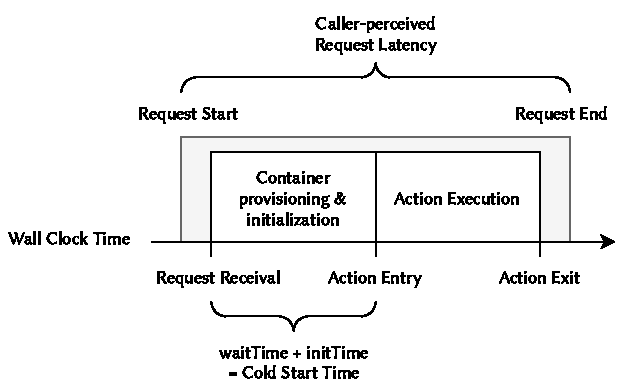
\includegraphics{figures/EvaluationTimeMeasurement.pdf}
    \caption{The two time measurements we use to evaluate the system's performance.}
    \label{fig:evaluation-time-measurement}
\end{figure}

There are a two papers which describe their approach to measuring serverless performance in more detail, which we use as a basis for our evaluation.

\begin{itemize}
    \item \citeauthor{McGrath2017} use concurrency tests to evaluate a platform's ability to scale \cite{McGrath2017}. The concurrency test starts by issuing a request to the platform and reissues it as soon as it completes. At a fixed interval, it adds another request up to an upper bound. In this manner, the load increases over time until a plateau is reached, where an increase in requests no longer increases the number of completed requests per time unit.
    \item \citeauthor{Hall2019} characterize access patterns to serverless functions based on a real-world scenario. They describe three different patterns: Non-concurrent requests from a single client; multiple clients making a single request, possibly concurrent and multiple clients making multiple requests, also possibly concurrent \cite{Hall2019}.
\end{itemize}

Based on these, we use two similar tests to measure cold start times and throughput.

\begin{itemize}
    \item To measure cold start times we first configure OpenWhisk's deallocation time as 10 seconds. We can then send requests at intervals exceeding 10 seconds to always trigger cold starts. In order to measure the effect of concurrency on cold starts, we send $i$ number of concurrent requests, where $i$ iterates through the set $\{1,...,N\}$ and $N$ is an upper bound we determine during the tests. After each iteration, we wait for OpenWhisk to destroy all containers before continuing. That results in exactly $i$ concurrent cold starts on each iteration. This measurement will aid in answering research question 1.

    \item To evaluate the performance of the systems, we will run concurrent requests under various workloads consisting of either CPU- or I/O-bound actions, or both. In the mixed scenario, we use the approach by \citeauthor{McGrath2017} in their concurrency test, and pick workload types at random. This is to ensure that we evaluate the system for both types and close to a real-world scenario. It is also similar to the approach of \citeauthor{Hall2019}, in that we have multiple concurrent requests but multiple clients are replaced by diverse workload types. The isolated experiments help us evaluate the pure performance of the respective workload types. Finally, we will run a workload based on research data introduced in Chapter \ref{chapter:background} which simulates that of a cloud provider. We will go into more detail for each measurement in the respective sections. These experiments will help us answer research question 2.

    \item This test aims to evaluate, what the resource costs of actions are, specifically their code size and the amount of memory they consume while being held in-memory; ready for execution. We use the Docker API to measure each container's memory footprint and measure the allocated memory of the WebAssembly executor process to infer the costs for WebAssembly containers. This measurement supports the answer to research question 3.
\end{itemize}

Finally, all measurements and the experience of the design phase will lead us to a conclusion on research question 4.

Our test procedure follows this pattern:

\begin{enumerate}
    \item Based on the latest available stable release of OpenWhisk, which is \inl{1.0.0}, compile the standalone version in our modified Wasm variant, as well as the unmodified vanilla version.
    \item Start the OpenWhisk variant under test on the test machine.
    \item Use the local \inl{wsk} command line tool to create the test action(s).
    \item From a separate machine, start the test procedure, which will send requests to the test machine.
\end{enumerate}

\subsection{Deployment}

We run our evaluation on an edge device as well as a \inl{x86\_64} server-class machine. The edge device is a Raspberry Pi Model 3B, which has 1 GB of RAM and is running the latest version of the 64-bit Raspberry Pi OS (version \inl{2020-08-20}). We are using the 64-bit version, because the \inl{wasmtime} runtime cannot be compiled for the 32-bit \inl{arm} architecture. The server has an Intel® Xeon® E3-1231 v3 (3.40 GHz) server-grade CPU with 4 physical cores and 8 logical threads. Mass storage is a Samsung SSD 850 EVO -- which is where Docker images are stored and loaded from -- and it has 8 GB of RAM and is running Ubuntu 20.04.2 LTS.

Due to difficulties in deploying OpenWhisk on the Raspberry Pi with Kubernetes and ansible, we use the standalone Java version for evaluation. The standalone version uses OpenWhisk's \emph{lean} components for internal messaging and load balancing. These are components written specifically for deployment on resource-constrained devices. Since we are not benchmarking OpenWhisk itself, but rather the underlying container technology, we do not believe this to be a threat to validity.

\section{Cold Start}

\begin{figure}
    \begin{center}
        %% Creator: Matplotlib, PGF backend
%%
%% To include the figure in your LaTeX document, write
%%   \input{<filename>.pgf}
%%
%% Make sure the required packages are loaded in your preamble
%%   \usepackage{pgf}
%%
%% and, on pdftex
%%   \usepackage[utf8]{inputenc}\DeclareUnicodeCharacter{2212}{-}
%%
%% or, on luatex and xetex
%%   \usepackage{unicode-math}
%%
%% Figures using additional raster images can only be included by \input if
%% they are in the same directory as the main LaTeX file. For loading figures
%% from other directories you can use the `import` package
%%   \usepackage{import}
%%
%% and then include the figures with
%%   \import{<path to file>}{<filename>.pgf}
%%
%% Matplotlib used the following preamble
%%   \usepackage{fontspec}
%%
\begingroup%
\makeatletter%
\begin{pgfpicture}%
\pgfpathrectangle{\pgfpointorigin}{\pgfqpoint{5.809079in}{3.485447in}}%
\pgfusepath{use as bounding box, clip}%
\begin{pgfscope}%
\pgfsetbuttcap%
\pgfsetmiterjoin%
\definecolor{currentfill}{rgb}{1.000000,1.000000,1.000000}%
\pgfsetfillcolor{currentfill}%
\pgfsetlinewidth{0.000000pt}%
\definecolor{currentstroke}{rgb}{1.000000,1.000000,1.000000}%
\pgfsetstrokecolor{currentstroke}%
\pgfsetdash{}{0pt}%
\pgfpathmoveto{\pgfqpoint{0.000000in}{0.000000in}}%
\pgfpathlineto{\pgfqpoint{5.809079in}{0.000000in}}%
\pgfpathlineto{\pgfqpoint{5.809079in}{3.485447in}}%
\pgfpathlineto{\pgfqpoint{0.000000in}{3.485447in}}%
\pgfpathclose%
\pgfusepath{fill}%
\end{pgfscope}%
\begin{pgfscope}%
\pgfsetbuttcap%
\pgfsetmiterjoin%
\definecolor{currentfill}{rgb}{0.917647,0.917647,0.949020}%
\pgfsetfillcolor{currentfill}%
\pgfsetlinewidth{0.000000pt}%
\definecolor{currentstroke}{rgb}{0.000000,0.000000,0.000000}%
\pgfsetstrokecolor{currentstroke}%
\pgfsetstrokeopacity{0.000000}%
\pgfsetdash{}{0pt}%
\pgfpathmoveto{\pgfqpoint{0.838500in}{0.652833in}}%
\pgfpathlineto{\pgfqpoint{5.629079in}{0.652833in}}%
\pgfpathlineto{\pgfqpoint{5.629079in}{3.104781in}}%
\pgfpathlineto{\pgfqpoint{0.838500in}{3.104781in}}%
\pgfpathclose%
\pgfusepath{fill}%
\end{pgfscope}%
\begin{pgfscope}%
\pgfpathrectangle{\pgfqpoint{0.838500in}{0.652833in}}{\pgfqpoint{4.790579in}{2.451948in}}%
\pgfusepath{clip}%
\pgfsetroundcap%
\pgfsetroundjoin%
\pgfsetlinewidth{1.003750pt}%
\definecolor{currentstroke}{rgb}{1.000000,1.000000,1.000000}%
\pgfsetstrokecolor{currentstroke}%
\pgfsetdash{}{0pt}%
\pgfpathmoveto{\pgfqpoint{1.056254in}{0.652833in}}%
\pgfpathlineto{\pgfqpoint{1.056254in}{3.104781in}}%
\pgfusepath{stroke}%
\end{pgfscope}%
\begin{pgfscope}%
\definecolor{textcolor}{rgb}{0.150000,0.150000,0.150000}%
\pgfsetstrokecolor{textcolor}%
\pgfsetfillcolor{textcolor}%
\pgftext[x=1.056254in,y=0.520889in,,top]{\color{textcolor}\rmfamily\fontsize{11.000000}{13.200000}\selectfont \(\displaystyle {2}\)}%
\end{pgfscope}%
\begin{pgfscope}%
\pgfpathrectangle{\pgfqpoint{0.838500in}{0.652833in}}{\pgfqpoint{4.790579in}{2.451948in}}%
\pgfusepath{clip}%
\pgfsetroundcap%
\pgfsetroundjoin%
\pgfsetlinewidth{1.003750pt}%
\definecolor{currentstroke}{rgb}{1.000000,1.000000,1.000000}%
\pgfsetstrokecolor{currentstroke}%
\pgfsetdash{}{0pt}%
\pgfpathmoveto{\pgfqpoint{1.600638in}{0.652833in}}%
\pgfpathlineto{\pgfqpoint{1.600638in}{3.104781in}}%
\pgfusepath{stroke}%
\end{pgfscope}%
\begin{pgfscope}%
\definecolor{textcolor}{rgb}{0.150000,0.150000,0.150000}%
\pgfsetstrokecolor{textcolor}%
\pgfsetfillcolor{textcolor}%
\pgftext[x=1.600638in,y=0.520889in,,top]{\color{textcolor}\rmfamily\fontsize{11.000000}{13.200000}\selectfont \(\displaystyle {3}\)}%
\end{pgfscope}%
\begin{pgfscope}%
\pgfpathrectangle{\pgfqpoint{0.838500in}{0.652833in}}{\pgfqpoint{4.790579in}{2.451948in}}%
\pgfusepath{clip}%
\pgfsetroundcap%
\pgfsetroundjoin%
\pgfsetlinewidth{1.003750pt}%
\definecolor{currentstroke}{rgb}{1.000000,1.000000,1.000000}%
\pgfsetstrokecolor{currentstroke}%
\pgfsetdash{}{0pt}%
\pgfpathmoveto{\pgfqpoint{2.145022in}{0.652833in}}%
\pgfpathlineto{\pgfqpoint{2.145022in}{3.104781in}}%
\pgfusepath{stroke}%
\end{pgfscope}%
\begin{pgfscope}%
\definecolor{textcolor}{rgb}{0.150000,0.150000,0.150000}%
\pgfsetstrokecolor{textcolor}%
\pgfsetfillcolor{textcolor}%
\pgftext[x=2.145022in,y=0.520889in,,top]{\color{textcolor}\rmfamily\fontsize{11.000000}{13.200000}\selectfont \(\displaystyle {4}\)}%
\end{pgfscope}%
\begin{pgfscope}%
\pgfpathrectangle{\pgfqpoint{0.838500in}{0.652833in}}{\pgfqpoint{4.790579in}{2.451948in}}%
\pgfusepath{clip}%
\pgfsetroundcap%
\pgfsetroundjoin%
\pgfsetlinewidth{1.003750pt}%
\definecolor{currentstroke}{rgb}{1.000000,1.000000,1.000000}%
\pgfsetstrokecolor{currentstroke}%
\pgfsetdash{}{0pt}%
\pgfpathmoveto{\pgfqpoint{2.689405in}{0.652833in}}%
\pgfpathlineto{\pgfqpoint{2.689405in}{3.104781in}}%
\pgfusepath{stroke}%
\end{pgfscope}%
\begin{pgfscope}%
\definecolor{textcolor}{rgb}{0.150000,0.150000,0.150000}%
\pgfsetstrokecolor{textcolor}%
\pgfsetfillcolor{textcolor}%
\pgftext[x=2.689405in,y=0.520889in,,top]{\color{textcolor}\rmfamily\fontsize{11.000000}{13.200000}\selectfont \(\displaystyle {5}\)}%
\end{pgfscope}%
\begin{pgfscope}%
\pgfpathrectangle{\pgfqpoint{0.838500in}{0.652833in}}{\pgfqpoint{4.790579in}{2.451948in}}%
\pgfusepath{clip}%
\pgfsetroundcap%
\pgfsetroundjoin%
\pgfsetlinewidth{1.003750pt}%
\definecolor{currentstroke}{rgb}{1.000000,1.000000,1.000000}%
\pgfsetstrokecolor{currentstroke}%
\pgfsetdash{}{0pt}%
\pgfpathmoveto{\pgfqpoint{3.233789in}{0.652833in}}%
\pgfpathlineto{\pgfqpoint{3.233789in}{3.104781in}}%
\pgfusepath{stroke}%
\end{pgfscope}%
\begin{pgfscope}%
\definecolor{textcolor}{rgb}{0.150000,0.150000,0.150000}%
\pgfsetstrokecolor{textcolor}%
\pgfsetfillcolor{textcolor}%
\pgftext[x=3.233789in,y=0.520889in,,top]{\color{textcolor}\rmfamily\fontsize{11.000000}{13.200000}\selectfont \(\displaystyle {6}\)}%
\end{pgfscope}%
\begin{pgfscope}%
\pgfpathrectangle{\pgfqpoint{0.838500in}{0.652833in}}{\pgfqpoint{4.790579in}{2.451948in}}%
\pgfusepath{clip}%
\pgfsetroundcap%
\pgfsetroundjoin%
\pgfsetlinewidth{1.003750pt}%
\definecolor{currentstroke}{rgb}{1.000000,1.000000,1.000000}%
\pgfsetstrokecolor{currentstroke}%
\pgfsetdash{}{0pt}%
\pgfpathmoveto{\pgfqpoint{3.778173in}{0.652833in}}%
\pgfpathlineto{\pgfqpoint{3.778173in}{3.104781in}}%
\pgfusepath{stroke}%
\end{pgfscope}%
\begin{pgfscope}%
\definecolor{textcolor}{rgb}{0.150000,0.150000,0.150000}%
\pgfsetstrokecolor{textcolor}%
\pgfsetfillcolor{textcolor}%
\pgftext[x=3.778173in,y=0.520889in,,top]{\color{textcolor}\rmfamily\fontsize{11.000000}{13.200000}\selectfont \(\displaystyle {7}\)}%
\end{pgfscope}%
\begin{pgfscope}%
\pgfpathrectangle{\pgfqpoint{0.838500in}{0.652833in}}{\pgfqpoint{4.790579in}{2.451948in}}%
\pgfusepath{clip}%
\pgfsetroundcap%
\pgfsetroundjoin%
\pgfsetlinewidth{1.003750pt}%
\definecolor{currentstroke}{rgb}{1.000000,1.000000,1.000000}%
\pgfsetstrokecolor{currentstroke}%
\pgfsetdash{}{0pt}%
\pgfpathmoveto{\pgfqpoint{4.322557in}{0.652833in}}%
\pgfpathlineto{\pgfqpoint{4.322557in}{3.104781in}}%
\pgfusepath{stroke}%
\end{pgfscope}%
\begin{pgfscope}%
\definecolor{textcolor}{rgb}{0.150000,0.150000,0.150000}%
\pgfsetstrokecolor{textcolor}%
\pgfsetfillcolor{textcolor}%
\pgftext[x=4.322557in,y=0.520889in,,top]{\color{textcolor}\rmfamily\fontsize{11.000000}{13.200000}\selectfont \(\displaystyle {8}\)}%
\end{pgfscope}%
\begin{pgfscope}%
\pgfpathrectangle{\pgfqpoint{0.838500in}{0.652833in}}{\pgfqpoint{4.790579in}{2.451948in}}%
\pgfusepath{clip}%
\pgfsetroundcap%
\pgfsetroundjoin%
\pgfsetlinewidth{1.003750pt}%
\definecolor{currentstroke}{rgb}{1.000000,1.000000,1.000000}%
\pgfsetstrokecolor{currentstroke}%
\pgfsetdash{}{0pt}%
\pgfpathmoveto{\pgfqpoint{4.866941in}{0.652833in}}%
\pgfpathlineto{\pgfqpoint{4.866941in}{3.104781in}}%
\pgfusepath{stroke}%
\end{pgfscope}%
\begin{pgfscope}%
\definecolor{textcolor}{rgb}{0.150000,0.150000,0.150000}%
\pgfsetstrokecolor{textcolor}%
\pgfsetfillcolor{textcolor}%
\pgftext[x=4.866941in,y=0.520889in,,top]{\color{textcolor}\rmfamily\fontsize{11.000000}{13.200000}\selectfont \(\displaystyle {9}\)}%
\end{pgfscope}%
\begin{pgfscope}%
\pgfpathrectangle{\pgfqpoint{0.838500in}{0.652833in}}{\pgfqpoint{4.790579in}{2.451948in}}%
\pgfusepath{clip}%
\pgfsetroundcap%
\pgfsetroundjoin%
\pgfsetlinewidth{1.003750pt}%
\definecolor{currentstroke}{rgb}{1.000000,1.000000,1.000000}%
\pgfsetstrokecolor{currentstroke}%
\pgfsetdash{}{0pt}%
\pgfpathmoveto{\pgfqpoint{5.411325in}{0.652833in}}%
\pgfpathlineto{\pgfqpoint{5.411325in}{3.104781in}}%
\pgfusepath{stroke}%
\end{pgfscope}%
\begin{pgfscope}%
\definecolor{textcolor}{rgb}{0.150000,0.150000,0.150000}%
\pgfsetstrokecolor{textcolor}%
\pgfsetfillcolor{textcolor}%
\pgftext[x=5.411325in,y=0.520889in,,top]{\color{textcolor}\rmfamily\fontsize{11.000000}{13.200000}\selectfont \(\displaystyle {10}\)}%
\end{pgfscope}%
\begin{pgfscope}%
\definecolor{textcolor}{rgb}{0.150000,0.150000,0.150000}%
\pgfsetstrokecolor{textcolor}%
\pgfsetfillcolor{textcolor}%
\pgftext[x=3.233789in,y=0.329667in,,top]{\color{textcolor}\rmfamily\fontsize{12.000000}{14.400000}\selectfont Number of Concurrent Requests}%
\end{pgfscope}%
\begin{pgfscope}%
\pgfpathrectangle{\pgfqpoint{0.838500in}{0.652833in}}{\pgfqpoint{4.790579in}{2.451948in}}%
\pgfusepath{clip}%
\pgfsetroundcap%
\pgfsetroundjoin%
\pgfsetlinewidth{1.003750pt}%
\definecolor{currentstroke}{rgb}{1.000000,1.000000,1.000000}%
\pgfsetstrokecolor{currentstroke}%
\pgfsetdash{}{0pt}%
\pgfpathmoveto{\pgfqpoint{0.838500in}{0.852552in}}%
\pgfpathlineto{\pgfqpoint{5.629079in}{0.852552in}}%
\pgfusepath{stroke}%
\end{pgfscope}%
\begin{pgfscope}%
\definecolor{textcolor}{rgb}{0.150000,0.150000,0.150000}%
\pgfsetstrokecolor{textcolor}%
\pgfsetfillcolor{textcolor}%
\pgftext[x=0.630514in, y=0.799538in, left, base]{\color{textcolor}\rmfamily\fontsize{11.000000}{13.200000}\selectfont \(\displaystyle {1}\)}%
\end{pgfscope}%
\begin{pgfscope}%
\pgfpathrectangle{\pgfqpoint{0.838500in}{0.652833in}}{\pgfqpoint{4.790579in}{2.451948in}}%
\pgfusepath{clip}%
\pgfsetroundcap%
\pgfsetroundjoin%
\pgfsetlinewidth{1.003750pt}%
\definecolor{currentstroke}{rgb}{1.000000,1.000000,1.000000}%
\pgfsetstrokecolor{currentstroke}%
\pgfsetdash{}{0pt}%
\pgfpathmoveto{\pgfqpoint{0.838500in}{1.570656in}}%
\pgfpathlineto{\pgfqpoint{5.629079in}{1.570656in}}%
\pgfusepath{stroke}%
\end{pgfscope}%
\begin{pgfscope}%
\definecolor{textcolor}{rgb}{0.150000,0.150000,0.150000}%
\pgfsetstrokecolor{textcolor}%
\pgfsetfillcolor{textcolor}%
\pgftext[x=0.554472in, y=1.517642in, left, base]{\color{textcolor}\rmfamily\fontsize{11.000000}{13.200000}\selectfont \(\displaystyle {10}\)}%
\end{pgfscope}%
\begin{pgfscope}%
\pgfpathrectangle{\pgfqpoint{0.838500in}{0.652833in}}{\pgfqpoint{4.790579in}{2.451948in}}%
\pgfusepath{clip}%
\pgfsetroundcap%
\pgfsetroundjoin%
\pgfsetlinewidth{1.003750pt}%
\definecolor{currentstroke}{rgb}{1.000000,1.000000,1.000000}%
\pgfsetstrokecolor{currentstroke}%
\pgfsetdash{}{0pt}%
\pgfpathmoveto{\pgfqpoint{0.838500in}{2.288759in}}%
\pgfpathlineto{\pgfqpoint{5.629079in}{2.288759in}}%
\pgfusepath{stroke}%
\end{pgfscope}%
\begin{pgfscope}%
\definecolor{textcolor}{rgb}{0.150000,0.150000,0.150000}%
\pgfsetstrokecolor{textcolor}%
\pgfsetfillcolor{textcolor}%
\pgftext[x=0.478430in, y=2.235745in, left, base]{\color{textcolor}\rmfamily\fontsize{11.000000}{13.200000}\selectfont \(\displaystyle {100}\)}%
\end{pgfscope}%
\begin{pgfscope}%
\pgfpathrectangle{\pgfqpoint{0.838500in}{0.652833in}}{\pgfqpoint{4.790579in}{2.451948in}}%
\pgfusepath{clip}%
\pgfsetroundcap%
\pgfsetroundjoin%
\pgfsetlinewidth{1.003750pt}%
\definecolor{currentstroke}{rgb}{1.000000,1.000000,1.000000}%
\pgfsetstrokecolor{currentstroke}%
\pgfsetdash{}{0pt}%
\pgfpathmoveto{\pgfqpoint{0.838500in}{3.006863in}}%
\pgfpathlineto{\pgfqpoint{5.629079in}{3.006863in}}%
\pgfusepath{stroke}%
\end{pgfscope}%
\begin{pgfscope}%
\definecolor{textcolor}{rgb}{0.150000,0.150000,0.150000}%
\pgfsetstrokecolor{textcolor}%
\pgfsetfillcolor{textcolor}%
\pgftext[x=0.402389in, y=2.953849in, left, base]{\color{textcolor}\rmfamily\fontsize{11.000000}{13.200000}\selectfont \(\displaystyle {1000}\)}%
\end{pgfscope}%
\begin{pgfscope}%
\definecolor{textcolor}{rgb}{0.150000,0.150000,0.150000}%
\pgfsetstrokecolor{textcolor}%
\pgfsetfillcolor{textcolor}%
\pgftext[x=0.346833in,y=1.878807in,,bottom,rotate=90.000000]{\color{textcolor}\rmfamily\fontsize{12.000000}{14.400000}\selectfont Cold Start Time (s)}%
\end{pgfscope}%
\begin{pgfscope}%
\pgfpathrectangle{\pgfqpoint{0.838500in}{0.652833in}}{\pgfqpoint{4.790579in}{2.451948in}}%
\pgfusepath{clip}%
\pgfsetbuttcap%
\pgfsetroundjoin%
\definecolor{currentfill}{rgb}{0.298039,0.447059,0.690196}%
\pgfsetfillcolor{currentfill}%
\pgfsetfillopacity{0.200000}%
\pgfsetlinewidth{1.003750pt}%
\definecolor{currentstroke}{rgb}{0.298039,0.447059,0.690196}%
\pgfsetstrokecolor{currentstroke}%
\pgfsetstrokeopacity{0.200000}%
\pgfsetdash{}{0pt}%
\pgfsys@defobject{currentmarker}{\pgfqpoint{1.056254in}{2.172360in}}{\pgfqpoint{3.233789in}{2.993329in}}{%
\pgfpathmoveto{\pgfqpoint{1.056254in}{2.324139in}}%
\pgfpathlineto{\pgfqpoint{1.056254in}{2.172360in}}%
\pgfpathlineto{\pgfqpoint{1.600638in}{2.617017in}}%
\pgfpathlineto{\pgfqpoint{2.145022in}{2.765187in}}%
\pgfpathlineto{\pgfqpoint{2.689405in}{2.783994in}}%
\pgfpathlineto{\pgfqpoint{3.233789in}{2.894340in}}%
\pgfpathlineto{\pgfqpoint{3.233789in}{2.993329in}}%
\pgfpathlineto{\pgfqpoint{3.233789in}{2.993329in}}%
\pgfpathlineto{\pgfqpoint{2.689405in}{2.824707in}}%
\pgfpathlineto{\pgfqpoint{2.145022in}{2.787349in}}%
\pgfpathlineto{\pgfqpoint{1.600638in}{2.685089in}}%
\pgfpathlineto{\pgfqpoint{1.056254in}{2.324139in}}%
\pgfpathclose%
\pgfusepath{stroke,fill}%
}%
\begin{pgfscope}%
\pgfsys@transformshift{0.000000in}{0.000000in}%
\pgfsys@useobject{currentmarker}{}%
\end{pgfscope}%
\end{pgfscope}%
\begin{pgfscope}%
\pgfpathrectangle{\pgfqpoint{0.838500in}{0.652833in}}{\pgfqpoint{4.790579in}{2.451948in}}%
\pgfusepath{clip}%
\pgfsetbuttcap%
\pgfsetroundjoin%
\definecolor{currentfill}{rgb}{0.866667,0.517647,0.321569}%
\pgfsetfillcolor{currentfill}%
\pgfsetfillopacity{0.200000}%
\pgfsetlinewidth{1.003750pt}%
\definecolor{currentstroke}{rgb}{0.866667,0.517647,0.321569}%
\pgfsetstrokecolor{currentstroke}%
\pgfsetstrokeopacity{0.200000}%
\pgfsetdash{}{0pt}%
\pgfsys@defobject{currentmarker}{\pgfqpoint{1.056254in}{0.769620in}}{\pgfqpoint{5.411325in}{1.225222in}}{%
\pgfpathmoveto{\pgfqpoint{1.056254in}{0.891632in}}%
\pgfpathlineto{\pgfqpoint{1.056254in}{0.769620in}}%
\pgfpathlineto{\pgfqpoint{1.600638in}{0.800888in}}%
\pgfpathlineto{\pgfqpoint{2.145022in}{0.876069in}}%
\pgfpathlineto{\pgfqpoint{2.689405in}{0.894834in}}%
\pgfpathlineto{\pgfqpoint{3.233789in}{0.962273in}}%
\pgfpathlineto{\pgfqpoint{3.778173in}{1.005434in}}%
\pgfpathlineto{\pgfqpoint{4.322557in}{1.045228in}}%
\pgfpathlineto{\pgfqpoint{4.866941in}{1.085869in}}%
\pgfpathlineto{\pgfqpoint{5.411325in}{1.106664in}}%
\pgfpathlineto{\pgfqpoint{5.411325in}{1.225222in}}%
\pgfpathlineto{\pgfqpoint{5.411325in}{1.225222in}}%
\pgfpathlineto{\pgfqpoint{4.866941in}{1.201412in}}%
\pgfpathlineto{\pgfqpoint{4.322557in}{1.160588in}}%
\pgfpathlineto{\pgfqpoint{3.778173in}{1.131849in}}%
\pgfpathlineto{\pgfqpoint{3.233789in}{1.098477in}}%
\pgfpathlineto{\pgfqpoint{2.689405in}{1.048224in}}%
\pgfpathlineto{\pgfqpoint{2.145022in}{1.022591in}}%
\pgfpathlineto{\pgfqpoint{1.600638in}{0.953226in}}%
\pgfpathlineto{\pgfqpoint{1.056254in}{0.891632in}}%
\pgfpathclose%
\pgfusepath{stroke,fill}%
}%
\begin{pgfscope}%
\pgfsys@transformshift{0.000000in}{0.000000in}%
\pgfsys@useobject{currentmarker}{}%
\end{pgfscope}%
\end{pgfscope}%
\begin{pgfscope}%
\pgfpathrectangle{\pgfqpoint{0.838500in}{0.652833in}}{\pgfqpoint{4.790579in}{2.451948in}}%
\pgfusepath{clip}%
\pgfsetbuttcap%
\pgfsetroundjoin%
\definecolor{currentfill}{rgb}{0.333333,0.658824,0.407843}%
\pgfsetfillcolor{currentfill}%
\pgfsetfillopacity{0.200000}%
\pgfsetlinewidth{1.003750pt}%
\definecolor{currentstroke}{rgb}{0.333333,0.658824,0.407843}%
\pgfsetstrokecolor{currentstroke}%
\pgfsetstrokeopacity{0.200000}%
\pgfsetdash{}{0pt}%
\pgfsys@defobject{currentmarker}{\pgfqpoint{1.056254in}{0.797433in}}{\pgfqpoint{5.411325in}{1.241799in}}{%
\pgfpathmoveto{\pgfqpoint{1.056254in}{0.913158in}}%
\pgfpathlineto{\pgfqpoint{1.056254in}{0.797433in}}%
\pgfpathlineto{\pgfqpoint{1.600638in}{0.857413in}}%
\pgfpathlineto{\pgfqpoint{2.145022in}{0.903827in}}%
\pgfpathlineto{\pgfqpoint{2.689405in}{0.929824in}}%
\pgfpathlineto{\pgfqpoint{3.233789in}{0.995250in}}%
\pgfpathlineto{\pgfqpoint{3.778173in}{1.026805in}}%
\pgfpathlineto{\pgfqpoint{4.322557in}{1.095586in}}%
\pgfpathlineto{\pgfqpoint{4.866941in}{1.126451in}}%
\pgfpathlineto{\pgfqpoint{5.411325in}{1.106303in}}%
\pgfpathlineto{\pgfqpoint{5.411325in}{1.217145in}}%
\pgfpathlineto{\pgfqpoint{5.411325in}{1.217145in}}%
\pgfpathlineto{\pgfqpoint{4.866941in}{1.241799in}}%
\pgfpathlineto{\pgfqpoint{4.322557in}{1.224390in}}%
\pgfpathlineto{\pgfqpoint{3.778173in}{1.146712in}}%
\pgfpathlineto{\pgfqpoint{3.233789in}{1.117544in}}%
\pgfpathlineto{\pgfqpoint{2.689405in}{1.074488in}}%
\pgfpathlineto{\pgfqpoint{2.145022in}{1.035239in}}%
\pgfpathlineto{\pgfqpoint{1.600638in}{0.991901in}}%
\pgfpathlineto{\pgfqpoint{1.056254in}{0.913158in}}%
\pgfpathclose%
\pgfusepath{stroke,fill}%
}%
\begin{pgfscope}%
\pgfsys@transformshift{0.000000in}{0.000000in}%
\pgfsys@useobject{currentmarker}{}%
\end{pgfscope}%
\end{pgfscope}%
\begin{pgfscope}%
\pgfpathrectangle{\pgfqpoint{0.838500in}{0.652833in}}{\pgfqpoint{4.790579in}{2.451948in}}%
\pgfusepath{clip}%
\pgfsetbuttcap%
\pgfsetroundjoin%
\definecolor{currentfill}{rgb}{0.768627,0.305882,0.321569}%
\pgfsetfillcolor{currentfill}%
\pgfsetfillopacity{0.200000}%
\pgfsetlinewidth{1.003750pt}%
\definecolor{currentstroke}{rgb}{0.768627,0.305882,0.321569}%
\pgfsetstrokecolor{currentstroke}%
\pgfsetstrokeopacity{0.200000}%
\pgfsetdash{}{0pt}%
\pgfsys@defobject{currentmarker}{\pgfqpoint{1.056254in}{0.764285in}}{\pgfqpoint{5.411325in}{1.208755in}}{%
\pgfpathmoveto{\pgfqpoint{1.056254in}{1.004015in}}%
\pgfpathlineto{\pgfqpoint{1.056254in}{0.764285in}}%
\pgfpathlineto{\pgfqpoint{1.600638in}{0.804460in}}%
\pgfpathlineto{\pgfqpoint{2.145022in}{0.851179in}}%
\pgfpathlineto{\pgfqpoint{2.689405in}{0.904961in}}%
\pgfpathlineto{\pgfqpoint{3.233789in}{0.982472in}}%
\pgfpathlineto{\pgfqpoint{3.778173in}{0.998009in}}%
\pgfpathlineto{\pgfqpoint{4.322557in}{1.033494in}}%
\pgfpathlineto{\pgfqpoint{4.866941in}{1.065245in}}%
\pgfpathlineto{\pgfqpoint{5.411325in}{1.096361in}}%
\pgfpathlineto{\pgfqpoint{5.411325in}{1.208755in}}%
\pgfpathlineto{\pgfqpoint{5.411325in}{1.208755in}}%
\pgfpathlineto{\pgfqpoint{4.866941in}{1.181031in}}%
\pgfpathlineto{\pgfqpoint{4.322557in}{1.161609in}}%
\pgfpathlineto{\pgfqpoint{3.778173in}{1.133060in}}%
\pgfpathlineto{\pgfqpoint{3.233789in}{1.100743in}}%
\pgfpathlineto{\pgfqpoint{2.689405in}{1.049044in}}%
\pgfpathlineto{\pgfqpoint{2.145022in}{0.997383in}}%
\pgfpathlineto{\pgfqpoint{1.600638in}{0.944756in}}%
\pgfpathlineto{\pgfqpoint{1.056254in}{1.004015in}}%
\pgfpathclose%
\pgfusepath{stroke,fill}%
}%
\begin{pgfscope}%
\pgfsys@transformshift{0.000000in}{0.000000in}%
\pgfsys@useobject{currentmarker}{}%
\end{pgfscope}%
\end{pgfscope}%
\begin{pgfscope}%
\pgfpathrectangle{\pgfqpoint{0.838500in}{0.652833in}}{\pgfqpoint{4.790579in}{2.451948in}}%
\pgfusepath{clip}%
\pgfsetroundcap%
\pgfsetroundjoin%
\pgfsetlinewidth{1.505625pt}%
\definecolor{currentstroke}{rgb}{0.298039,0.447059,0.690196}%
\pgfsetstrokecolor{currentstroke}%
\pgfsetdash{}{0pt}%
\pgfpathmoveto{\pgfqpoint{1.056254in}{2.257393in}}%
\pgfpathlineto{\pgfqpoint{1.600638in}{2.652905in}}%
\pgfpathlineto{\pgfqpoint{2.145022in}{2.776462in}}%
\pgfpathlineto{\pgfqpoint{2.689405in}{2.805010in}}%
\pgfpathlineto{\pgfqpoint{3.233789in}{2.945834in}}%
\pgfusepath{stroke}%
\end{pgfscope}%
\begin{pgfscope}%
\pgfpathrectangle{\pgfqpoint{0.838500in}{0.652833in}}{\pgfqpoint{4.790579in}{2.451948in}}%
\pgfusepath{clip}%
\pgfsetbuttcap%
\pgfsetroundjoin%
\definecolor{currentfill}{rgb}{0.298039,0.447059,0.690196}%
\pgfsetfillcolor{currentfill}%
\pgfsetlinewidth{0.752812pt}%
\definecolor{currentstroke}{rgb}{1.000000,1.000000,1.000000}%
\pgfsetstrokecolor{currentstroke}%
\pgfsetdash{}{0pt}%
\pgfsys@defobject{currentmarker}{\pgfqpoint{-0.041667in}{-0.041667in}}{\pgfqpoint{0.041667in}{0.041667in}}{%
\pgfpathmoveto{\pgfqpoint{0.000000in}{-0.041667in}}%
\pgfpathcurveto{\pgfqpoint{0.011050in}{-0.041667in}}{\pgfqpoint{0.021649in}{-0.037276in}}{\pgfqpoint{0.029463in}{-0.029463in}}%
\pgfpathcurveto{\pgfqpoint{0.037276in}{-0.021649in}}{\pgfqpoint{0.041667in}{-0.011050in}}{\pgfqpoint{0.041667in}{0.000000in}}%
\pgfpathcurveto{\pgfqpoint{0.041667in}{0.011050in}}{\pgfqpoint{0.037276in}{0.021649in}}{\pgfqpoint{0.029463in}{0.029463in}}%
\pgfpathcurveto{\pgfqpoint{0.021649in}{0.037276in}}{\pgfqpoint{0.011050in}{0.041667in}}{\pgfqpoint{0.000000in}{0.041667in}}%
\pgfpathcurveto{\pgfqpoint{-0.011050in}{0.041667in}}{\pgfqpoint{-0.021649in}{0.037276in}}{\pgfqpoint{-0.029463in}{0.029463in}}%
\pgfpathcurveto{\pgfqpoint{-0.037276in}{0.021649in}}{\pgfqpoint{-0.041667in}{0.011050in}}{\pgfqpoint{-0.041667in}{0.000000in}}%
\pgfpathcurveto{\pgfqpoint{-0.041667in}{-0.011050in}}{\pgfqpoint{-0.037276in}{-0.021649in}}{\pgfqpoint{-0.029463in}{-0.029463in}}%
\pgfpathcurveto{\pgfqpoint{-0.021649in}{-0.037276in}}{\pgfqpoint{-0.011050in}{-0.041667in}}{\pgfqpoint{0.000000in}{-0.041667in}}%
\pgfpathclose%
\pgfusepath{stroke,fill}%
}%
\begin{pgfscope}%
\pgfsys@transformshift{1.056254in}{2.257393in}%
\pgfsys@useobject{currentmarker}{}%
\end{pgfscope}%
\begin{pgfscope}%
\pgfsys@transformshift{1.600638in}{2.652905in}%
\pgfsys@useobject{currentmarker}{}%
\end{pgfscope}%
\begin{pgfscope}%
\pgfsys@transformshift{2.145022in}{2.776462in}%
\pgfsys@useobject{currentmarker}{}%
\end{pgfscope}%
\begin{pgfscope}%
\pgfsys@transformshift{2.689405in}{2.805010in}%
\pgfsys@useobject{currentmarker}{}%
\end{pgfscope}%
\begin{pgfscope}%
\pgfsys@transformshift{3.233789in}{2.945834in}%
\pgfsys@useobject{currentmarker}{}%
\end{pgfscope}%
\end{pgfscope}%
\begin{pgfscope}%
\pgfpathrectangle{\pgfqpoint{0.838500in}{0.652833in}}{\pgfqpoint{4.790579in}{2.451948in}}%
\pgfusepath{clip}%
\pgfsetroundcap%
\pgfsetroundjoin%
\pgfsetlinewidth{1.505625pt}%
\definecolor{currentstroke}{rgb}{0.866667,0.517647,0.321569}%
\pgfsetstrokecolor{currentstroke}%
\pgfsetdash{}{0pt}%
\pgfpathmoveto{\pgfqpoint{1.056254in}{0.839577in}}%
\pgfpathlineto{\pgfqpoint{1.600638in}{0.885099in}}%
\pgfpathlineto{\pgfqpoint{2.145022in}{0.956176in}}%
\pgfpathlineto{\pgfqpoint{2.689405in}{0.985485in}}%
\pgfpathlineto{\pgfqpoint{3.233789in}{1.039553in}}%
\pgfpathlineto{\pgfqpoint{3.778173in}{1.076010in}}%
\pgfpathlineto{\pgfqpoint{4.322557in}{1.108138in}}%
\pgfpathlineto{\pgfqpoint{4.866941in}{1.146225in}}%
\pgfpathlineto{\pgfqpoint{5.411325in}{1.172083in}}%
\pgfusepath{stroke}%
\end{pgfscope}%
\begin{pgfscope}%
\pgfpathrectangle{\pgfqpoint{0.838500in}{0.652833in}}{\pgfqpoint{4.790579in}{2.451948in}}%
\pgfusepath{clip}%
\pgfsetbuttcap%
\pgfsetroundjoin%
\definecolor{currentfill}{rgb}{0.866667,0.517647,0.321569}%
\pgfsetfillcolor{currentfill}%
\pgfsetlinewidth{0.752812pt}%
\definecolor{currentstroke}{rgb}{1.000000,1.000000,1.000000}%
\pgfsetstrokecolor{currentstroke}%
\pgfsetdash{}{0pt}%
\pgfsys@defobject{currentmarker}{\pgfqpoint{-0.041667in}{-0.041667in}}{\pgfqpoint{0.041667in}{0.041667in}}{%
\pgfpathmoveto{\pgfqpoint{0.000000in}{-0.041667in}}%
\pgfpathcurveto{\pgfqpoint{0.011050in}{-0.041667in}}{\pgfqpoint{0.021649in}{-0.037276in}}{\pgfqpoint{0.029463in}{-0.029463in}}%
\pgfpathcurveto{\pgfqpoint{0.037276in}{-0.021649in}}{\pgfqpoint{0.041667in}{-0.011050in}}{\pgfqpoint{0.041667in}{0.000000in}}%
\pgfpathcurveto{\pgfqpoint{0.041667in}{0.011050in}}{\pgfqpoint{0.037276in}{0.021649in}}{\pgfqpoint{0.029463in}{0.029463in}}%
\pgfpathcurveto{\pgfqpoint{0.021649in}{0.037276in}}{\pgfqpoint{0.011050in}{0.041667in}}{\pgfqpoint{0.000000in}{0.041667in}}%
\pgfpathcurveto{\pgfqpoint{-0.011050in}{0.041667in}}{\pgfqpoint{-0.021649in}{0.037276in}}{\pgfqpoint{-0.029463in}{0.029463in}}%
\pgfpathcurveto{\pgfqpoint{-0.037276in}{0.021649in}}{\pgfqpoint{-0.041667in}{0.011050in}}{\pgfqpoint{-0.041667in}{0.000000in}}%
\pgfpathcurveto{\pgfqpoint{-0.041667in}{-0.011050in}}{\pgfqpoint{-0.037276in}{-0.021649in}}{\pgfqpoint{-0.029463in}{-0.029463in}}%
\pgfpathcurveto{\pgfqpoint{-0.021649in}{-0.037276in}}{\pgfqpoint{-0.011050in}{-0.041667in}}{\pgfqpoint{0.000000in}{-0.041667in}}%
\pgfpathclose%
\pgfusepath{stroke,fill}%
}%
\begin{pgfscope}%
\pgfsys@transformshift{1.056254in}{0.839577in}%
\pgfsys@useobject{currentmarker}{}%
\end{pgfscope}%
\begin{pgfscope}%
\pgfsys@transformshift{1.600638in}{0.885099in}%
\pgfsys@useobject{currentmarker}{}%
\end{pgfscope}%
\begin{pgfscope}%
\pgfsys@transformshift{2.145022in}{0.956176in}%
\pgfsys@useobject{currentmarker}{}%
\end{pgfscope}%
\begin{pgfscope}%
\pgfsys@transformshift{2.689405in}{0.985485in}%
\pgfsys@useobject{currentmarker}{}%
\end{pgfscope}%
\begin{pgfscope}%
\pgfsys@transformshift{3.233789in}{1.039553in}%
\pgfsys@useobject{currentmarker}{}%
\end{pgfscope}%
\begin{pgfscope}%
\pgfsys@transformshift{3.778173in}{1.076010in}%
\pgfsys@useobject{currentmarker}{}%
\end{pgfscope}%
\begin{pgfscope}%
\pgfsys@transformshift{4.322557in}{1.108138in}%
\pgfsys@useobject{currentmarker}{}%
\end{pgfscope}%
\begin{pgfscope}%
\pgfsys@transformshift{4.866941in}{1.146225in}%
\pgfsys@useobject{currentmarker}{}%
\end{pgfscope}%
\begin{pgfscope}%
\pgfsys@transformshift{5.411325in}{1.172083in}%
\pgfsys@useobject{currentmarker}{}%
\end{pgfscope}%
\end{pgfscope}%
\begin{pgfscope}%
\pgfpathrectangle{\pgfqpoint{0.838500in}{0.652833in}}{\pgfqpoint{4.790579in}{2.451948in}}%
\pgfusepath{clip}%
\pgfsetroundcap%
\pgfsetroundjoin%
\pgfsetlinewidth{1.505625pt}%
\definecolor{currentstroke}{rgb}{0.333333,0.658824,0.407843}%
\pgfsetstrokecolor{currentstroke}%
\pgfsetdash{}{0pt}%
\pgfpathmoveto{\pgfqpoint{1.056254in}{0.860633in}}%
\pgfpathlineto{\pgfqpoint{1.600638in}{0.929986in}}%
\pgfpathlineto{\pgfqpoint{2.145022in}{0.976682in}}%
\pgfpathlineto{\pgfqpoint{2.689405in}{1.014088in}}%
\pgfpathlineto{\pgfqpoint{3.233789in}{1.063494in}}%
\pgfpathlineto{\pgfqpoint{3.778173in}{1.093703in}}%
\pgfpathlineto{\pgfqpoint{4.322557in}{1.166269in}}%
\pgfpathlineto{\pgfqpoint{4.866941in}{1.192378in}}%
\pgfpathlineto{\pgfqpoint{5.411325in}{1.168084in}}%
\pgfusepath{stroke}%
\end{pgfscope}%
\begin{pgfscope}%
\pgfpathrectangle{\pgfqpoint{0.838500in}{0.652833in}}{\pgfqpoint{4.790579in}{2.451948in}}%
\pgfusepath{clip}%
\pgfsetbuttcap%
\pgfsetroundjoin%
\definecolor{currentfill}{rgb}{0.333333,0.658824,0.407843}%
\pgfsetfillcolor{currentfill}%
\pgfsetlinewidth{0.752812pt}%
\definecolor{currentstroke}{rgb}{1.000000,1.000000,1.000000}%
\pgfsetstrokecolor{currentstroke}%
\pgfsetdash{}{0pt}%
\pgfsys@defobject{currentmarker}{\pgfqpoint{-0.041667in}{-0.041667in}}{\pgfqpoint{0.041667in}{0.041667in}}{%
\pgfpathmoveto{\pgfqpoint{0.000000in}{-0.041667in}}%
\pgfpathcurveto{\pgfqpoint{0.011050in}{-0.041667in}}{\pgfqpoint{0.021649in}{-0.037276in}}{\pgfqpoint{0.029463in}{-0.029463in}}%
\pgfpathcurveto{\pgfqpoint{0.037276in}{-0.021649in}}{\pgfqpoint{0.041667in}{-0.011050in}}{\pgfqpoint{0.041667in}{0.000000in}}%
\pgfpathcurveto{\pgfqpoint{0.041667in}{0.011050in}}{\pgfqpoint{0.037276in}{0.021649in}}{\pgfqpoint{0.029463in}{0.029463in}}%
\pgfpathcurveto{\pgfqpoint{0.021649in}{0.037276in}}{\pgfqpoint{0.011050in}{0.041667in}}{\pgfqpoint{0.000000in}{0.041667in}}%
\pgfpathcurveto{\pgfqpoint{-0.011050in}{0.041667in}}{\pgfqpoint{-0.021649in}{0.037276in}}{\pgfqpoint{-0.029463in}{0.029463in}}%
\pgfpathcurveto{\pgfqpoint{-0.037276in}{0.021649in}}{\pgfqpoint{-0.041667in}{0.011050in}}{\pgfqpoint{-0.041667in}{0.000000in}}%
\pgfpathcurveto{\pgfqpoint{-0.041667in}{-0.011050in}}{\pgfqpoint{-0.037276in}{-0.021649in}}{\pgfqpoint{-0.029463in}{-0.029463in}}%
\pgfpathcurveto{\pgfqpoint{-0.021649in}{-0.037276in}}{\pgfqpoint{-0.011050in}{-0.041667in}}{\pgfqpoint{0.000000in}{-0.041667in}}%
\pgfpathclose%
\pgfusepath{stroke,fill}%
}%
\begin{pgfscope}%
\pgfsys@transformshift{1.056254in}{0.860633in}%
\pgfsys@useobject{currentmarker}{}%
\end{pgfscope}%
\begin{pgfscope}%
\pgfsys@transformshift{1.600638in}{0.929986in}%
\pgfsys@useobject{currentmarker}{}%
\end{pgfscope}%
\begin{pgfscope}%
\pgfsys@transformshift{2.145022in}{0.976682in}%
\pgfsys@useobject{currentmarker}{}%
\end{pgfscope}%
\begin{pgfscope}%
\pgfsys@transformshift{2.689405in}{1.014088in}%
\pgfsys@useobject{currentmarker}{}%
\end{pgfscope}%
\begin{pgfscope}%
\pgfsys@transformshift{3.233789in}{1.063494in}%
\pgfsys@useobject{currentmarker}{}%
\end{pgfscope}%
\begin{pgfscope}%
\pgfsys@transformshift{3.778173in}{1.093703in}%
\pgfsys@useobject{currentmarker}{}%
\end{pgfscope}%
\begin{pgfscope}%
\pgfsys@transformshift{4.322557in}{1.166269in}%
\pgfsys@useobject{currentmarker}{}%
\end{pgfscope}%
\begin{pgfscope}%
\pgfsys@transformshift{4.866941in}{1.192378in}%
\pgfsys@useobject{currentmarker}{}%
\end{pgfscope}%
\begin{pgfscope}%
\pgfsys@transformshift{5.411325in}{1.168084in}%
\pgfsys@useobject{currentmarker}{}%
\end{pgfscope}%
\end{pgfscope}%
\begin{pgfscope}%
\pgfpathrectangle{\pgfqpoint{0.838500in}{0.652833in}}{\pgfqpoint{4.790579in}{2.451948in}}%
\pgfusepath{clip}%
\pgfsetroundcap%
\pgfsetroundjoin%
\pgfsetlinewidth{1.505625pt}%
\definecolor{currentstroke}{rgb}{0.768627,0.305882,0.321569}%
\pgfsetstrokecolor{currentstroke}%
\pgfsetdash{}{0pt}%
\pgfpathmoveto{\pgfqpoint{1.056254in}{0.890599in}}%
\pgfpathlineto{\pgfqpoint{1.600638in}{0.883314in}}%
\pgfpathlineto{\pgfqpoint{2.145022in}{0.933354in}}%
\pgfpathlineto{\pgfqpoint{2.689405in}{0.985648in}}%
\pgfpathlineto{\pgfqpoint{3.233789in}{1.047318in}}%
\pgfpathlineto{\pgfqpoint{3.778173in}{1.074582in}}%
\pgfpathlineto{\pgfqpoint{4.322557in}{1.104197in}}%
\pgfpathlineto{\pgfqpoint{4.866941in}{1.129536in}}%
\pgfpathlineto{\pgfqpoint{5.411325in}{1.159968in}}%
\pgfusepath{stroke}%
\end{pgfscope}%
\begin{pgfscope}%
\pgfpathrectangle{\pgfqpoint{0.838500in}{0.652833in}}{\pgfqpoint{4.790579in}{2.451948in}}%
\pgfusepath{clip}%
\pgfsetbuttcap%
\pgfsetroundjoin%
\definecolor{currentfill}{rgb}{0.768627,0.305882,0.321569}%
\pgfsetfillcolor{currentfill}%
\pgfsetlinewidth{0.752812pt}%
\definecolor{currentstroke}{rgb}{1.000000,1.000000,1.000000}%
\pgfsetstrokecolor{currentstroke}%
\pgfsetdash{}{0pt}%
\pgfsys@defobject{currentmarker}{\pgfqpoint{-0.041667in}{-0.041667in}}{\pgfqpoint{0.041667in}{0.041667in}}{%
\pgfpathmoveto{\pgfqpoint{0.000000in}{-0.041667in}}%
\pgfpathcurveto{\pgfqpoint{0.011050in}{-0.041667in}}{\pgfqpoint{0.021649in}{-0.037276in}}{\pgfqpoint{0.029463in}{-0.029463in}}%
\pgfpathcurveto{\pgfqpoint{0.037276in}{-0.021649in}}{\pgfqpoint{0.041667in}{-0.011050in}}{\pgfqpoint{0.041667in}{0.000000in}}%
\pgfpathcurveto{\pgfqpoint{0.041667in}{0.011050in}}{\pgfqpoint{0.037276in}{0.021649in}}{\pgfqpoint{0.029463in}{0.029463in}}%
\pgfpathcurveto{\pgfqpoint{0.021649in}{0.037276in}}{\pgfqpoint{0.011050in}{0.041667in}}{\pgfqpoint{0.000000in}{0.041667in}}%
\pgfpathcurveto{\pgfqpoint{-0.011050in}{0.041667in}}{\pgfqpoint{-0.021649in}{0.037276in}}{\pgfqpoint{-0.029463in}{0.029463in}}%
\pgfpathcurveto{\pgfqpoint{-0.037276in}{0.021649in}}{\pgfqpoint{-0.041667in}{0.011050in}}{\pgfqpoint{-0.041667in}{0.000000in}}%
\pgfpathcurveto{\pgfqpoint{-0.041667in}{-0.011050in}}{\pgfqpoint{-0.037276in}{-0.021649in}}{\pgfqpoint{-0.029463in}{-0.029463in}}%
\pgfpathcurveto{\pgfqpoint{-0.021649in}{-0.037276in}}{\pgfqpoint{-0.011050in}{-0.041667in}}{\pgfqpoint{0.000000in}{-0.041667in}}%
\pgfpathclose%
\pgfusepath{stroke,fill}%
}%
\begin{pgfscope}%
\pgfsys@transformshift{1.056254in}{0.890599in}%
\pgfsys@useobject{currentmarker}{}%
\end{pgfscope}%
\begin{pgfscope}%
\pgfsys@transformshift{1.600638in}{0.883314in}%
\pgfsys@useobject{currentmarker}{}%
\end{pgfscope}%
\begin{pgfscope}%
\pgfsys@transformshift{2.145022in}{0.933354in}%
\pgfsys@useobject{currentmarker}{}%
\end{pgfscope}%
\begin{pgfscope}%
\pgfsys@transformshift{2.689405in}{0.985648in}%
\pgfsys@useobject{currentmarker}{}%
\end{pgfscope}%
\begin{pgfscope}%
\pgfsys@transformshift{3.233789in}{1.047318in}%
\pgfsys@useobject{currentmarker}{}%
\end{pgfscope}%
\begin{pgfscope}%
\pgfsys@transformshift{3.778173in}{1.074582in}%
\pgfsys@useobject{currentmarker}{}%
\end{pgfscope}%
\begin{pgfscope}%
\pgfsys@transformshift{4.322557in}{1.104197in}%
\pgfsys@useobject{currentmarker}{}%
\end{pgfscope}%
\begin{pgfscope}%
\pgfsys@transformshift{4.866941in}{1.129536in}%
\pgfsys@useobject{currentmarker}{}%
\end{pgfscope}%
\begin{pgfscope}%
\pgfsys@transformshift{5.411325in}{1.159968in}%
\pgfsys@useobject{currentmarker}{}%
\end{pgfscope}%
\end{pgfscope}%
\begin{pgfscope}%
\pgfsetrectcap%
\pgfsetmiterjoin%
\pgfsetlinewidth{1.254687pt}%
\definecolor{currentstroke}{rgb}{1.000000,1.000000,1.000000}%
\pgfsetstrokecolor{currentstroke}%
\pgfsetdash{}{0pt}%
\pgfpathmoveto{\pgfqpoint{0.838500in}{0.652833in}}%
\pgfpathlineto{\pgfqpoint{0.838500in}{3.104781in}}%
\pgfusepath{stroke}%
\end{pgfscope}%
\begin{pgfscope}%
\pgfsetrectcap%
\pgfsetmiterjoin%
\pgfsetlinewidth{1.254687pt}%
\definecolor{currentstroke}{rgb}{1.000000,1.000000,1.000000}%
\pgfsetstrokecolor{currentstroke}%
\pgfsetdash{}{0pt}%
\pgfpathmoveto{\pgfqpoint{5.629079in}{0.652833in}}%
\pgfpathlineto{\pgfqpoint{5.629079in}{3.104781in}}%
\pgfusepath{stroke}%
\end{pgfscope}%
\begin{pgfscope}%
\pgfsetrectcap%
\pgfsetmiterjoin%
\pgfsetlinewidth{1.254687pt}%
\definecolor{currentstroke}{rgb}{1.000000,1.000000,1.000000}%
\pgfsetstrokecolor{currentstroke}%
\pgfsetdash{}{0pt}%
\pgfpathmoveto{\pgfqpoint{0.838500in}{0.652833in}}%
\pgfpathlineto{\pgfqpoint{5.629079in}{0.652833in}}%
\pgfusepath{stroke}%
\end{pgfscope}%
\begin{pgfscope}%
\pgfsetrectcap%
\pgfsetmiterjoin%
\pgfsetlinewidth{1.254687pt}%
\definecolor{currentstroke}{rgb}{1.000000,1.000000,1.000000}%
\pgfsetstrokecolor{currentstroke}%
\pgfsetdash{}{0pt}%
\pgfpathmoveto{\pgfqpoint{0.838500in}{3.104781in}}%
\pgfpathlineto{\pgfqpoint{5.629079in}{3.104781in}}%
\pgfusepath{stroke}%
\end{pgfscope}%
\begin{pgfscope}%
\definecolor{textcolor}{rgb}{0.150000,0.150000,0.150000}%
\pgfsetstrokecolor{textcolor}%
\pgfsetfillcolor{textcolor}%
\pgftext[x=3.233789in,y=3.188114in,,base]{\color{textcolor}\rmfamily\fontsize{12.000000}{14.400000}\selectfont Raspberry Pi: Cold Start Test}%
\end{pgfscope}%
\begin{pgfscope}%
\pgfsetbuttcap%
\pgfsetmiterjoin%
\definecolor{currentfill}{rgb}{0.917647,0.917647,0.949020}%
\pgfsetfillcolor{currentfill}%
\pgfsetfillopacity{0.800000}%
\pgfsetlinewidth{1.003750pt}%
\definecolor{currentstroke}{rgb}{0.800000,0.800000,0.800000}%
\pgfsetstrokecolor{currentstroke}%
\pgfsetstrokeopacity{0.800000}%
\pgfsetdash{}{0pt}%
\pgfpathmoveto{\pgfqpoint{4.384093in}{2.130670in}}%
\pgfpathlineto{\pgfqpoint{5.522134in}{2.130670in}}%
\pgfpathquadraticcurveto{\pgfqpoint{5.552690in}{2.130670in}}{\pgfqpoint{5.552690in}{2.161226in}}%
\pgfpathlineto{\pgfqpoint{5.552690in}{2.997836in}}%
\pgfpathquadraticcurveto{\pgfqpoint{5.552690in}{3.028392in}}{\pgfqpoint{5.522134in}{3.028392in}}%
\pgfpathlineto{\pgfqpoint{4.384093in}{3.028392in}}%
\pgfpathquadraticcurveto{\pgfqpoint{4.353537in}{3.028392in}}{\pgfqpoint{4.353537in}{2.997836in}}%
\pgfpathlineto{\pgfqpoint{4.353537in}{2.161226in}}%
\pgfpathquadraticcurveto{\pgfqpoint{4.353537in}{2.130670in}}{\pgfqpoint{4.384093in}{2.130670in}}%
\pgfpathclose%
\pgfusepath{stroke,fill}%
\end{pgfscope}%
\begin{pgfscope}%
\pgfsetroundcap%
\pgfsetroundjoin%
\pgfsetlinewidth{1.505625pt}%
\definecolor{currentstroke}{rgb}{0.298039,0.447059,0.690196}%
\pgfsetstrokecolor{currentstroke}%
\pgfsetdash{}{0pt}%
\pgfpathmoveto{\pgfqpoint{4.414648in}{2.913808in}}%
\pgfpathlineto{\pgfqpoint{4.720204in}{2.913808in}}%
\pgfusepath{stroke}%
\end{pgfscope}%
\begin{pgfscope}%
\pgfsetbuttcap%
\pgfsetroundjoin%
\definecolor{currentfill}{rgb}{0.298039,0.447059,0.690196}%
\pgfsetfillcolor{currentfill}%
\pgfsetlinewidth{0.752812pt}%
\definecolor{currentstroke}{rgb}{1.000000,1.000000,1.000000}%
\pgfsetstrokecolor{currentstroke}%
\pgfsetdash{}{0pt}%
\pgfsys@defobject{currentmarker}{\pgfqpoint{-0.041667in}{-0.041667in}}{\pgfqpoint{0.041667in}{0.041667in}}{%
\pgfpathmoveto{\pgfqpoint{0.000000in}{-0.041667in}}%
\pgfpathcurveto{\pgfqpoint{0.011050in}{-0.041667in}}{\pgfqpoint{0.021649in}{-0.037276in}}{\pgfqpoint{0.029463in}{-0.029463in}}%
\pgfpathcurveto{\pgfqpoint{0.037276in}{-0.021649in}}{\pgfqpoint{0.041667in}{-0.011050in}}{\pgfqpoint{0.041667in}{0.000000in}}%
\pgfpathcurveto{\pgfqpoint{0.041667in}{0.011050in}}{\pgfqpoint{0.037276in}{0.021649in}}{\pgfqpoint{0.029463in}{0.029463in}}%
\pgfpathcurveto{\pgfqpoint{0.021649in}{0.037276in}}{\pgfqpoint{0.011050in}{0.041667in}}{\pgfqpoint{0.000000in}{0.041667in}}%
\pgfpathcurveto{\pgfqpoint{-0.011050in}{0.041667in}}{\pgfqpoint{-0.021649in}{0.037276in}}{\pgfqpoint{-0.029463in}{0.029463in}}%
\pgfpathcurveto{\pgfqpoint{-0.037276in}{0.021649in}}{\pgfqpoint{-0.041667in}{0.011050in}}{\pgfqpoint{-0.041667in}{0.000000in}}%
\pgfpathcurveto{\pgfqpoint{-0.041667in}{-0.011050in}}{\pgfqpoint{-0.037276in}{-0.021649in}}{\pgfqpoint{-0.029463in}{-0.029463in}}%
\pgfpathcurveto{\pgfqpoint{-0.021649in}{-0.037276in}}{\pgfqpoint{-0.011050in}{-0.041667in}}{\pgfqpoint{0.000000in}{-0.041667in}}%
\pgfpathclose%
\pgfusepath{stroke,fill}%
}%
\begin{pgfscope}%
\pgfsys@transformshift{4.567426in}{2.913808in}%
\pgfsys@useobject{currentmarker}{}%
\end{pgfscope}%
\end{pgfscope}%
\begin{pgfscope}%
\definecolor{textcolor}{rgb}{0.150000,0.150000,0.150000}%
\pgfsetstrokecolor{textcolor}%
\pgfsetfillcolor{textcolor}%
\pgftext[x=4.842426in,y=2.860336in,left,base]{\color{textcolor}\rmfamily\fontsize{11.000000}{13.200000}\selectfont docker}%
\end{pgfscope}%
\begin{pgfscope}%
\pgfsetroundcap%
\pgfsetroundjoin%
\pgfsetlinewidth{1.505625pt}%
\definecolor{currentstroke}{rgb}{0.866667,0.517647,0.321569}%
\pgfsetstrokecolor{currentstroke}%
\pgfsetdash{}{0pt}%
\pgfpathmoveto{\pgfqpoint{4.414648in}{2.700836in}}%
\pgfpathlineto{\pgfqpoint{4.720204in}{2.700836in}}%
\pgfusepath{stroke}%
\end{pgfscope}%
\begin{pgfscope}%
\pgfsetbuttcap%
\pgfsetroundjoin%
\definecolor{currentfill}{rgb}{0.866667,0.517647,0.321569}%
\pgfsetfillcolor{currentfill}%
\pgfsetlinewidth{0.752812pt}%
\definecolor{currentstroke}{rgb}{1.000000,1.000000,1.000000}%
\pgfsetstrokecolor{currentstroke}%
\pgfsetdash{}{0pt}%
\pgfsys@defobject{currentmarker}{\pgfqpoint{-0.041667in}{-0.041667in}}{\pgfqpoint{0.041667in}{0.041667in}}{%
\pgfpathmoveto{\pgfqpoint{0.000000in}{-0.041667in}}%
\pgfpathcurveto{\pgfqpoint{0.011050in}{-0.041667in}}{\pgfqpoint{0.021649in}{-0.037276in}}{\pgfqpoint{0.029463in}{-0.029463in}}%
\pgfpathcurveto{\pgfqpoint{0.037276in}{-0.021649in}}{\pgfqpoint{0.041667in}{-0.011050in}}{\pgfqpoint{0.041667in}{0.000000in}}%
\pgfpathcurveto{\pgfqpoint{0.041667in}{0.011050in}}{\pgfqpoint{0.037276in}{0.021649in}}{\pgfqpoint{0.029463in}{0.029463in}}%
\pgfpathcurveto{\pgfqpoint{0.021649in}{0.037276in}}{\pgfqpoint{0.011050in}{0.041667in}}{\pgfqpoint{0.000000in}{0.041667in}}%
\pgfpathcurveto{\pgfqpoint{-0.011050in}{0.041667in}}{\pgfqpoint{-0.021649in}{0.037276in}}{\pgfqpoint{-0.029463in}{0.029463in}}%
\pgfpathcurveto{\pgfqpoint{-0.037276in}{0.021649in}}{\pgfqpoint{-0.041667in}{0.011050in}}{\pgfqpoint{-0.041667in}{0.000000in}}%
\pgfpathcurveto{\pgfqpoint{-0.041667in}{-0.011050in}}{\pgfqpoint{-0.037276in}{-0.021649in}}{\pgfqpoint{-0.029463in}{-0.029463in}}%
\pgfpathcurveto{\pgfqpoint{-0.021649in}{-0.037276in}}{\pgfqpoint{-0.011050in}{-0.041667in}}{\pgfqpoint{0.000000in}{-0.041667in}}%
\pgfpathclose%
\pgfusepath{stroke,fill}%
}%
\begin{pgfscope}%
\pgfsys@transformshift{4.567426in}{2.700836in}%
\pgfsys@useobject{currentmarker}{}%
\end{pgfscope}%
\end{pgfscope}%
\begin{pgfscope}%
\definecolor{textcolor}{rgb}{0.150000,0.150000,0.150000}%
\pgfsetstrokecolor{textcolor}%
\pgfsetfillcolor{textcolor}%
\pgftext[x=4.842426in,y=2.647364in,left,base]{\color{textcolor}\rmfamily\fontsize{11.000000}{13.200000}\selectfont wasmtime}%
\end{pgfscope}%
\begin{pgfscope}%
\pgfsetroundcap%
\pgfsetroundjoin%
\pgfsetlinewidth{1.505625pt}%
\definecolor{currentstroke}{rgb}{0.333333,0.658824,0.407843}%
\pgfsetstrokecolor{currentstroke}%
\pgfsetdash{}{0pt}%
\pgfpathmoveto{\pgfqpoint{4.414648in}{2.487864in}}%
\pgfpathlineto{\pgfqpoint{4.720204in}{2.487864in}}%
\pgfusepath{stroke}%
\end{pgfscope}%
\begin{pgfscope}%
\pgfsetbuttcap%
\pgfsetroundjoin%
\definecolor{currentfill}{rgb}{0.333333,0.658824,0.407843}%
\pgfsetfillcolor{currentfill}%
\pgfsetlinewidth{0.752812pt}%
\definecolor{currentstroke}{rgb}{1.000000,1.000000,1.000000}%
\pgfsetstrokecolor{currentstroke}%
\pgfsetdash{}{0pt}%
\pgfsys@defobject{currentmarker}{\pgfqpoint{-0.041667in}{-0.041667in}}{\pgfqpoint{0.041667in}{0.041667in}}{%
\pgfpathmoveto{\pgfqpoint{0.000000in}{-0.041667in}}%
\pgfpathcurveto{\pgfqpoint{0.011050in}{-0.041667in}}{\pgfqpoint{0.021649in}{-0.037276in}}{\pgfqpoint{0.029463in}{-0.029463in}}%
\pgfpathcurveto{\pgfqpoint{0.037276in}{-0.021649in}}{\pgfqpoint{0.041667in}{-0.011050in}}{\pgfqpoint{0.041667in}{0.000000in}}%
\pgfpathcurveto{\pgfqpoint{0.041667in}{0.011050in}}{\pgfqpoint{0.037276in}{0.021649in}}{\pgfqpoint{0.029463in}{0.029463in}}%
\pgfpathcurveto{\pgfqpoint{0.021649in}{0.037276in}}{\pgfqpoint{0.011050in}{0.041667in}}{\pgfqpoint{0.000000in}{0.041667in}}%
\pgfpathcurveto{\pgfqpoint{-0.011050in}{0.041667in}}{\pgfqpoint{-0.021649in}{0.037276in}}{\pgfqpoint{-0.029463in}{0.029463in}}%
\pgfpathcurveto{\pgfqpoint{-0.037276in}{0.021649in}}{\pgfqpoint{-0.041667in}{0.011050in}}{\pgfqpoint{-0.041667in}{0.000000in}}%
\pgfpathcurveto{\pgfqpoint{-0.041667in}{-0.011050in}}{\pgfqpoint{-0.037276in}{-0.021649in}}{\pgfqpoint{-0.029463in}{-0.029463in}}%
\pgfpathcurveto{\pgfqpoint{-0.021649in}{-0.037276in}}{\pgfqpoint{-0.011050in}{-0.041667in}}{\pgfqpoint{0.000000in}{-0.041667in}}%
\pgfpathclose%
\pgfusepath{stroke,fill}%
}%
\begin{pgfscope}%
\pgfsys@transformshift{4.567426in}{2.487864in}%
\pgfsys@useobject{currentmarker}{}%
\end{pgfscope}%
\end{pgfscope}%
\begin{pgfscope}%
\definecolor{textcolor}{rgb}{0.150000,0.150000,0.150000}%
\pgfsetstrokecolor{textcolor}%
\pgfsetfillcolor{textcolor}%
\pgftext[x=4.842426in,y=2.434392in,left,base]{\color{textcolor}\rmfamily\fontsize{11.000000}{13.200000}\selectfont wasmer}%
\end{pgfscope}%
\begin{pgfscope}%
\pgfsetroundcap%
\pgfsetroundjoin%
\pgfsetlinewidth{1.505625pt}%
\definecolor{currentstroke}{rgb}{0.768627,0.305882,0.321569}%
\pgfsetstrokecolor{currentstroke}%
\pgfsetdash{}{0pt}%
\pgfpathmoveto{\pgfqpoint{4.414648in}{2.274892in}}%
\pgfpathlineto{\pgfqpoint{4.720204in}{2.274892in}}%
\pgfusepath{stroke}%
\end{pgfscope}%
\begin{pgfscope}%
\pgfsetbuttcap%
\pgfsetroundjoin%
\definecolor{currentfill}{rgb}{0.768627,0.305882,0.321569}%
\pgfsetfillcolor{currentfill}%
\pgfsetlinewidth{0.752812pt}%
\definecolor{currentstroke}{rgb}{1.000000,1.000000,1.000000}%
\pgfsetstrokecolor{currentstroke}%
\pgfsetdash{}{0pt}%
\pgfsys@defobject{currentmarker}{\pgfqpoint{-0.041667in}{-0.041667in}}{\pgfqpoint{0.041667in}{0.041667in}}{%
\pgfpathmoveto{\pgfqpoint{0.000000in}{-0.041667in}}%
\pgfpathcurveto{\pgfqpoint{0.011050in}{-0.041667in}}{\pgfqpoint{0.021649in}{-0.037276in}}{\pgfqpoint{0.029463in}{-0.029463in}}%
\pgfpathcurveto{\pgfqpoint{0.037276in}{-0.021649in}}{\pgfqpoint{0.041667in}{-0.011050in}}{\pgfqpoint{0.041667in}{0.000000in}}%
\pgfpathcurveto{\pgfqpoint{0.041667in}{0.011050in}}{\pgfqpoint{0.037276in}{0.021649in}}{\pgfqpoint{0.029463in}{0.029463in}}%
\pgfpathcurveto{\pgfqpoint{0.021649in}{0.037276in}}{\pgfqpoint{0.011050in}{0.041667in}}{\pgfqpoint{0.000000in}{0.041667in}}%
\pgfpathcurveto{\pgfqpoint{-0.011050in}{0.041667in}}{\pgfqpoint{-0.021649in}{0.037276in}}{\pgfqpoint{-0.029463in}{0.029463in}}%
\pgfpathcurveto{\pgfqpoint{-0.037276in}{0.021649in}}{\pgfqpoint{-0.041667in}{0.011050in}}{\pgfqpoint{-0.041667in}{0.000000in}}%
\pgfpathcurveto{\pgfqpoint{-0.041667in}{-0.011050in}}{\pgfqpoint{-0.037276in}{-0.021649in}}{\pgfqpoint{-0.029463in}{-0.029463in}}%
\pgfpathcurveto{\pgfqpoint{-0.021649in}{-0.037276in}}{\pgfqpoint{-0.011050in}{-0.041667in}}{\pgfqpoint{0.000000in}{-0.041667in}}%
\pgfpathclose%
\pgfusepath{stroke,fill}%
}%
\begin{pgfscope}%
\pgfsys@transformshift{4.567426in}{2.274892in}%
\pgfsys@useobject{currentmarker}{}%
\end{pgfscope}%
\end{pgfscope}%
\begin{pgfscope}%
\definecolor{textcolor}{rgb}{0.150000,0.150000,0.150000}%
\pgfsetstrokecolor{textcolor}%
\pgfsetfillcolor{textcolor}%
\pgftext[x=4.842426in,y=2.221420in,left,base]{\color{textcolor}\rmfamily\fontsize{11.000000}{13.200000}\selectfont wamr}%
\end{pgfscope}%
\end{pgfpicture}%
\makeatother%
\endgroup%

    \end{center}
    \caption{The cold start time with a CPU-bound workload on a Raspberry Pi with both Docker and Wasm-based container runtimes. Note that the scale is logarithmic rather than linear, which may be surprising.}
    \label{fig:pi-cold-start-hash}
\end{figure}

During testing, various issues arose that we want to discuss, in order to give context about the deployment process. 
The first version of the test created our CPU-bound test action, called \inl{hash}, and then ran concurrent requests against OpenWhisk. In the result we noticed that for 5 and more concurrent requests, there were only 4 cold starts, independent of the underlying container runtime. It turned out that OpenWhisk would only create 4 containers and let other requests wait until one of the currently executing ones finished, so it could reuse the container. This is a fair optimization, but it does not let us test how 5 or more cold starts actually affect each other. So, instead of creating just one action, we create $N$ actions with different names but the same code. OpenWhisk will treat these as different actions and execute them in separate containers accordingly. However, it will still only allocate 4 containers at a time, something that does not appear to be configurable, waiting for one of them to complete before removing it and starting the next. Thus, the performance of the container removal operation also becomes important, as it blocks the provisioning of the next. It is implicitly part of the cold start time as we define it, since a container that needs to wait due to a slow remove operation from another container will have a higher \inl{waitTime}.
% This isn't reflected in the cold start latency, but we can look at the \inl{waitTime} annotation of OpenWhisk's activation record instead. It measures how long the activation spent waiting in OpenWhisk's queues. If the removal operation of Wasm runtimes is shorter than dockers, then Wasm action activations should have to spend less time waiting than their docker counterparts. Although, this value would also be affected by longer cold starts, so it can only provide a partial answer to this question.
% While testing the deployment with Wasm runtimes showed no performance issues, the vanilla OpenWhisk deployment was harder to test. 

OpenWhisk vanilla showed further issues in its default configuration. On every container start it executes a Docker pull operation, even if the image was locally present, which meant checking if the local image was up to date with the remote version, resulting in a higher \inl{waitTime} than necessary. Therefore, we turned this behavior off, since it is not an inherent part of the container startup, which improved cold start times.
% The Raspberry Pi we use has 913 MiB of total memory. The OS needs 210 MiB and OpenWhisk uses 185 MiB of memory after startup.

With two running Docker containers, OpenWhisk starts to approach the limits of the Raspberry Pi's memory. If OpenWhisk decides to start a third container, the system runs out of memory and freezes. Only after increasing the swap memory from the default 100 MiB to 1024 MiB were we able to test up to 6 concurrent cold starts.
This is reflected in Figure \ref{fig:pi-cold-start-hash} -- where we plotted the result of the cold start test -- with the Docker runtime having orders of magnitude higher cold start latencies than any of the Wasm executors. At 5 and 6 concurrent requests, the OpenWhisk logs showed Docker commands timing out and the testing time became unreasonably long -- as reflected in the figure -- which is why we stopped testing at that point.

Even at 2 concurrent requests, the Wasm executors have a cold start time of around one second, increasing with more requests. \inl{wasmtime} has the most consistent behaviour, followed by \inl{wamr} and \inl{wasmer}. Overall, the runtimes are similar in their startup performance, especially \inl{wasmtime} and \inl{wamr}, even though they are written in different languages and use different compilation strategies. The Wasm executors have, on average, less than 0.5\% the cold start time of Docker.

% Look at cold start time only for wasm runtimes, then reference the docker cold start time on an x86 host and draw a comparison. I.e. if the runtimes achieve a startup time of ~100ms on an edge device and docker achieves the same on an x86 host, then we can perhaps conclude that the Wasm runtimes are suitable/acceptable as container runtimes for the serverless edge.

\begin{figure}
    \begin{center}
        %% Creator: Matplotlib, PGF backend
%%
%% To include the figure in your LaTeX document, write
%%   \input{<filename>.pgf}
%%
%% Make sure the required packages are loaded in your preamble
%%   \usepackage{pgf}
%%
%% and, on pdftex
%%   \usepackage[utf8]{inputenc}\DeclareUnicodeCharacter{2212}{-}
%%
%% or, on luatex and xetex
%%   \usepackage{unicode-math}
%%
%% Figures using additional raster images can only be included by \input if
%% they are in the same directory as the main LaTeX file. For loading figures
%% from other directories you can use the `import` package
%%   \usepackage{import}
%%
%% and then include the figures with
%%   \import{<path to file>}{<filename>.pgf}
%%
%% Matplotlib used the following preamble
%%   \usepackage{fontspec}
%%
\begingroup%
\makeatletter%
\begin{pgfpicture}%
\pgfpathrectangle{\pgfpointorigin}{\pgfqpoint{5.809079in}{3.485447in}}%
\pgfusepath{use as bounding box, clip}%
\begin{pgfscope}%
\pgfsetbuttcap%
\pgfsetmiterjoin%
\definecolor{currentfill}{rgb}{1.000000,1.000000,1.000000}%
\pgfsetfillcolor{currentfill}%
\pgfsetlinewidth{0.000000pt}%
\definecolor{currentstroke}{rgb}{1.000000,1.000000,1.000000}%
\pgfsetstrokecolor{currentstroke}%
\pgfsetdash{}{0pt}%
\pgfpathmoveto{\pgfqpoint{0.000000in}{0.000000in}}%
\pgfpathlineto{\pgfqpoint{5.809079in}{0.000000in}}%
\pgfpathlineto{\pgfqpoint{5.809079in}{3.485447in}}%
\pgfpathlineto{\pgfqpoint{0.000000in}{3.485447in}}%
\pgfpathclose%
\pgfusepath{fill}%
\end{pgfscope}%
\begin{pgfscope}%
\pgfsetbuttcap%
\pgfsetmiterjoin%
\definecolor{currentfill}{rgb}{0.917647,0.917647,0.949020}%
\pgfsetfillcolor{currentfill}%
\pgfsetlinewidth{0.000000pt}%
\definecolor{currentstroke}{rgb}{0.000000,0.000000,0.000000}%
\pgfsetstrokecolor{currentstroke}%
\pgfsetstrokeopacity{0.000000}%
\pgfsetdash{}{0pt}%
\pgfpathmoveto{\pgfqpoint{0.838500in}{0.652833in}}%
\pgfpathlineto{\pgfqpoint{5.629079in}{0.652833in}}%
\pgfpathlineto{\pgfqpoint{5.629079in}{3.106447in}}%
\pgfpathlineto{\pgfqpoint{0.838500in}{3.106447in}}%
\pgfpathclose%
\pgfusepath{fill}%
\end{pgfscope}%
\begin{pgfscope}%
\pgfpathrectangle{\pgfqpoint{0.838500in}{0.652833in}}{\pgfqpoint{4.790579in}{2.453614in}}%
\pgfusepath{clip}%
\pgfsetroundcap%
\pgfsetroundjoin%
\pgfsetlinewidth{1.003750pt}%
\definecolor{currentstroke}{rgb}{1.000000,1.000000,1.000000}%
\pgfsetstrokecolor{currentstroke}%
\pgfsetdash{}{0pt}%
\pgfpathmoveto{\pgfqpoint{1.056254in}{0.652833in}}%
\pgfpathlineto{\pgfqpoint{1.056254in}{3.106447in}}%
\pgfusepath{stroke}%
\end{pgfscope}%
\begin{pgfscope}%
\definecolor{textcolor}{rgb}{0.150000,0.150000,0.150000}%
\pgfsetstrokecolor{textcolor}%
\pgfsetfillcolor{textcolor}%
\pgftext[x=1.056254in,y=0.520889in,,top]{\color{textcolor}\rmfamily\fontsize{11.000000}{13.200000}\selectfont \(\displaystyle {2}\)}%
\end{pgfscope}%
\begin{pgfscope}%
\pgfpathrectangle{\pgfqpoint{0.838500in}{0.652833in}}{\pgfqpoint{4.790579in}{2.453614in}}%
\pgfusepath{clip}%
\pgfsetroundcap%
\pgfsetroundjoin%
\pgfsetlinewidth{1.003750pt}%
\definecolor{currentstroke}{rgb}{1.000000,1.000000,1.000000}%
\pgfsetstrokecolor{currentstroke}%
\pgfsetdash{}{0pt}%
\pgfpathmoveto{\pgfqpoint{1.600638in}{0.652833in}}%
\pgfpathlineto{\pgfqpoint{1.600638in}{3.106447in}}%
\pgfusepath{stroke}%
\end{pgfscope}%
\begin{pgfscope}%
\definecolor{textcolor}{rgb}{0.150000,0.150000,0.150000}%
\pgfsetstrokecolor{textcolor}%
\pgfsetfillcolor{textcolor}%
\pgftext[x=1.600638in,y=0.520889in,,top]{\color{textcolor}\rmfamily\fontsize{11.000000}{13.200000}\selectfont \(\displaystyle {3}\)}%
\end{pgfscope}%
\begin{pgfscope}%
\pgfpathrectangle{\pgfqpoint{0.838500in}{0.652833in}}{\pgfqpoint{4.790579in}{2.453614in}}%
\pgfusepath{clip}%
\pgfsetroundcap%
\pgfsetroundjoin%
\pgfsetlinewidth{1.003750pt}%
\definecolor{currentstroke}{rgb}{1.000000,1.000000,1.000000}%
\pgfsetstrokecolor{currentstroke}%
\pgfsetdash{}{0pt}%
\pgfpathmoveto{\pgfqpoint{2.145022in}{0.652833in}}%
\pgfpathlineto{\pgfqpoint{2.145022in}{3.106447in}}%
\pgfusepath{stroke}%
\end{pgfscope}%
\begin{pgfscope}%
\definecolor{textcolor}{rgb}{0.150000,0.150000,0.150000}%
\pgfsetstrokecolor{textcolor}%
\pgfsetfillcolor{textcolor}%
\pgftext[x=2.145022in,y=0.520889in,,top]{\color{textcolor}\rmfamily\fontsize{11.000000}{13.200000}\selectfont \(\displaystyle {4}\)}%
\end{pgfscope}%
\begin{pgfscope}%
\pgfpathrectangle{\pgfqpoint{0.838500in}{0.652833in}}{\pgfqpoint{4.790579in}{2.453614in}}%
\pgfusepath{clip}%
\pgfsetroundcap%
\pgfsetroundjoin%
\pgfsetlinewidth{1.003750pt}%
\definecolor{currentstroke}{rgb}{1.000000,1.000000,1.000000}%
\pgfsetstrokecolor{currentstroke}%
\pgfsetdash{}{0pt}%
\pgfpathmoveto{\pgfqpoint{2.689405in}{0.652833in}}%
\pgfpathlineto{\pgfqpoint{2.689405in}{3.106447in}}%
\pgfusepath{stroke}%
\end{pgfscope}%
\begin{pgfscope}%
\definecolor{textcolor}{rgb}{0.150000,0.150000,0.150000}%
\pgfsetstrokecolor{textcolor}%
\pgfsetfillcolor{textcolor}%
\pgftext[x=2.689405in,y=0.520889in,,top]{\color{textcolor}\rmfamily\fontsize{11.000000}{13.200000}\selectfont \(\displaystyle {5}\)}%
\end{pgfscope}%
\begin{pgfscope}%
\pgfpathrectangle{\pgfqpoint{0.838500in}{0.652833in}}{\pgfqpoint{4.790579in}{2.453614in}}%
\pgfusepath{clip}%
\pgfsetroundcap%
\pgfsetroundjoin%
\pgfsetlinewidth{1.003750pt}%
\definecolor{currentstroke}{rgb}{1.000000,1.000000,1.000000}%
\pgfsetstrokecolor{currentstroke}%
\pgfsetdash{}{0pt}%
\pgfpathmoveto{\pgfqpoint{3.233789in}{0.652833in}}%
\pgfpathlineto{\pgfqpoint{3.233789in}{3.106447in}}%
\pgfusepath{stroke}%
\end{pgfscope}%
\begin{pgfscope}%
\definecolor{textcolor}{rgb}{0.150000,0.150000,0.150000}%
\pgfsetstrokecolor{textcolor}%
\pgfsetfillcolor{textcolor}%
\pgftext[x=3.233789in,y=0.520889in,,top]{\color{textcolor}\rmfamily\fontsize{11.000000}{13.200000}\selectfont \(\displaystyle {6}\)}%
\end{pgfscope}%
\begin{pgfscope}%
\pgfpathrectangle{\pgfqpoint{0.838500in}{0.652833in}}{\pgfqpoint{4.790579in}{2.453614in}}%
\pgfusepath{clip}%
\pgfsetroundcap%
\pgfsetroundjoin%
\pgfsetlinewidth{1.003750pt}%
\definecolor{currentstroke}{rgb}{1.000000,1.000000,1.000000}%
\pgfsetstrokecolor{currentstroke}%
\pgfsetdash{}{0pt}%
\pgfpathmoveto{\pgfqpoint{3.778173in}{0.652833in}}%
\pgfpathlineto{\pgfqpoint{3.778173in}{3.106447in}}%
\pgfusepath{stroke}%
\end{pgfscope}%
\begin{pgfscope}%
\definecolor{textcolor}{rgb}{0.150000,0.150000,0.150000}%
\pgfsetstrokecolor{textcolor}%
\pgfsetfillcolor{textcolor}%
\pgftext[x=3.778173in,y=0.520889in,,top]{\color{textcolor}\rmfamily\fontsize{11.000000}{13.200000}\selectfont \(\displaystyle {7}\)}%
\end{pgfscope}%
\begin{pgfscope}%
\pgfpathrectangle{\pgfqpoint{0.838500in}{0.652833in}}{\pgfqpoint{4.790579in}{2.453614in}}%
\pgfusepath{clip}%
\pgfsetroundcap%
\pgfsetroundjoin%
\pgfsetlinewidth{1.003750pt}%
\definecolor{currentstroke}{rgb}{1.000000,1.000000,1.000000}%
\pgfsetstrokecolor{currentstroke}%
\pgfsetdash{}{0pt}%
\pgfpathmoveto{\pgfqpoint{4.322557in}{0.652833in}}%
\pgfpathlineto{\pgfqpoint{4.322557in}{3.106447in}}%
\pgfusepath{stroke}%
\end{pgfscope}%
\begin{pgfscope}%
\definecolor{textcolor}{rgb}{0.150000,0.150000,0.150000}%
\pgfsetstrokecolor{textcolor}%
\pgfsetfillcolor{textcolor}%
\pgftext[x=4.322557in,y=0.520889in,,top]{\color{textcolor}\rmfamily\fontsize{11.000000}{13.200000}\selectfont \(\displaystyle {8}\)}%
\end{pgfscope}%
\begin{pgfscope}%
\pgfpathrectangle{\pgfqpoint{0.838500in}{0.652833in}}{\pgfqpoint{4.790579in}{2.453614in}}%
\pgfusepath{clip}%
\pgfsetroundcap%
\pgfsetroundjoin%
\pgfsetlinewidth{1.003750pt}%
\definecolor{currentstroke}{rgb}{1.000000,1.000000,1.000000}%
\pgfsetstrokecolor{currentstroke}%
\pgfsetdash{}{0pt}%
\pgfpathmoveto{\pgfqpoint{4.866941in}{0.652833in}}%
\pgfpathlineto{\pgfqpoint{4.866941in}{3.106447in}}%
\pgfusepath{stroke}%
\end{pgfscope}%
\begin{pgfscope}%
\definecolor{textcolor}{rgb}{0.150000,0.150000,0.150000}%
\pgfsetstrokecolor{textcolor}%
\pgfsetfillcolor{textcolor}%
\pgftext[x=4.866941in,y=0.520889in,,top]{\color{textcolor}\rmfamily\fontsize{11.000000}{13.200000}\selectfont \(\displaystyle {9}\)}%
\end{pgfscope}%
\begin{pgfscope}%
\pgfpathrectangle{\pgfqpoint{0.838500in}{0.652833in}}{\pgfqpoint{4.790579in}{2.453614in}}%
\pgfusepath{clip}%
\pgfsetroundcap%
\pgfsetroundjoin%
\pgfsetlinewidth{1.003750pt}%
\definecolor{currentstroke}{rgb}{1.000000,1.000000,1.000000}%
\pgfsetstrokecolor{currentstroke}%
\pgfsetdash{}{0pt}%
\pgfpathmoveto{\pgfqpoint{5.411325in}{0.652833in}}%
\pgfpathlineto{\pgfqpoint{5.411325in}{3.106447in}}%
\pgfusepath{stroke}%
\end{pgfscope}%
\begin{pgfscope}%
\definecolor{textcolor}{rgb}{0.150000,0.150000,0.150000}%
\pgfsetstrokecolor{textcolor}%
\pgfsetfillcolor{textcolor}%
\pgftext[x=5.411325in,y=0.520889in,,top]{\color{textcolor}\rmfamily\fontsize{11.000000}{13.200000}\selectfont \(\displaystyle {10}\)}%
\end{pgfscope}%
\begin{pgfscope}%
\definecolor{textcolor}{rgb}{0.150000,0.150000,0.150000}%
\pgfsetstrokecolor{textcolor}%
\pgfsetfillcolor{textcolor}%
\pgftext[x=3.233789in,y=0.329667in,,top]{\color{textcolor}\rmfamily\fontsize{12.000000}{14.400000}\selectfont Number of Concurrent Requests}%
\end{pgfscope}%
\begin{pgfscope}%
\pgfpathrectangle{\pgfqpoint{0.838500in}{0.652833in}}{\pgfqpoint{4.790579in}{2.453614in}}%
\pgfusepath{clip}%
\pgfsetroundcap%
\pgfsetroundjoin%
\pgfsetlinewidth{1.003750pt}%
\definecolor{currentstroke}{rgb}{1.000000,1.000000,1.000000}%
\pgfsetstrokecolor{currentstroke}%
\pgfsetdash{}{0pt}%
\pgfpathmoveto{\pgfqpoint{0.838500in}{1.238952in}}%
\pgfpathlineto{\pgfqpoint{5.629079in}{1.238952in}}%
\pgfusepath{stroke}%
\end{pgfscope}%
\begin{pgfscope}%
\definecolor{textcolor}{rgb}{0.150000,0.150000,0.150000}%
\pgfsetstrokecolor{textcolor}%
\pgfsetfillcolor{textcolor}%
\pgftext[x=0.478430in, y=1.185939in, left, base]{\color{textcolor}\rmfamily\fontsize{11.000000}{13.200000}\selectfont \(\displaystyle {100}\)}%
\end{pgfscope}%
\begin{pgfscope}%
\pgfpathrectangle{\pgfqpoint{0.838500in}{0.652833in}}{\pgfqpoint{4.790579in}{2.453614in}}%
\pgfusepath{clip}%
\pgfsetroundcap%
\pgfsetroundjoin%
\pgfsetlinewidth{1.003750pt}%
\definecolor{currentstroke}{rgb}{1.000000,1.000000,1.000000}%
\pgfsetstrokecolor{currentstroke}%
\pgfsetdash{}{0pt}%
\pgfpathmoveto{\pgfqpoint{0.838500in}{2.415423in}}%
\pgfpathlineto{\pgfqpoint{5.629079in}{2.415423in}}%
\pgfusepath{stroke}%
\end{pgfscope}%
\begin{pgfscope}%
\definecolor{textcolor}{rgb}{0.150000,0.150000,0.150000}%
\pgfsetstrokecolor{textcolor}%
\pgfsetfillcolor{textcolor}%
\pgftext[x=0.402389in, y=2.362409in, left, base]{\color{textcolor}\rmfamily\fontsize{11.000000}{13.200000}\selectfont \(\displaystyle {1000}\)}%
\end{pgfscope}%
\begin{pgfscope}%
\definecolor{textcolor}{rgb}{0.150000,0.150000,0.150000}%
\pgfsetstrokecolor{textcolor}%
\pgfsetfillcolor{textcolor}%
\pgftext[x=0.346833in,y=1.879640in,,bottom,rotate=90.000000]{\color{textcolor}\rmfamily\fontsize{12.000000}{14.400000}\selectfont Cold Start Time (ms)}%
\end{pgfscope}%
\begin{pgfscope}%
\pgfpathrectangle{\pgfqpoint{0.838500in}{0.652833in}}{\pgfqpoint{4.790579in}{2.453614in}}%
\pgfusepath{clip}%
\pgfsetbuttcap%
\pgfsetroundjoin%
\definecolor{currentfill}{rgb}{0.298039,0.447059,0.690196}%
\pgfsetfillcolor{currentfill}%
\pgfsetfillopacity{0.200000}%
\pgfsetlinewidth{1.003750pt}%
\definecolor{currentstroke}{rgb}{0.298039,0.447059,0.690196}%
\pgfsetstrokecolor{currentstroke}%
\pgfsetstrokeopacity{0.200000}%
\pgfsetdash{}{0pt}%
\pgfsys@defobject{currentmarker}{\pgfqpoint{1.056254in}{2.320682in}}{\pgfqpoint{5.411325in}{2.994919in}}{%
\pgfpathmoveto{\pgfqpoint{1.056254in}{2.357028in}}%
\pgfpathlineto{\pgfqpoint{1.056254in}{2.320682in}}%
\pgfpathlineto{\pgfqpoint{1.600638in}{2.432401in}}%
\pgfpathlineto{\pgfqpoint{2.145022in}{2.506492in}}%
\pgfpathlineto{\pgfqpoint{2.689405in}{2.537902in}}%
\pgfpathlineto{\pgfqpoint{3.233789in}{2.588329in}}%
\pgfpathlineto{\pgfqpoint{3.778173in}{2.678783in}}%
\pgfpathlineto{\pgfqpoint{4.322557in}{2.699714in}}%
\pgfpathlineto{\pgfqpoint{4.866941in}{2.774185in}}%
\pgfpathlineto{\pgfqpoint{5.411325in}{2.802959in}}%
\pgfpathlineto{\pgfqpoint{5.411325in}{2.994919in}}%
\pgfpathlineto{\pgfqpoint{5.411325in}{2.994919in}}%
\pgfpathlineto{\pgfqpoint{4.866941in}{2.960929in}}%
\pgfpathlineto{\pgfqpoint{4.322557in}{2.890461in}}%
\pgfpathlineto{\pgfqpoint{3.778173in}{2.858021in}}%
\pgfpathlineto{\pgfqpoint{3.233789in}{2.765889in}}%
\pgfpathlineto{\pgfqpoint{2.689405in}{2.682712in}}%
\pgfpathlineto{\pgfqpoint{2.145022in}{2.564008in}}%
\pgfpathlineto{\pgfqpoint{1.600638in}{2.495204in}}%
\pgfpathlineto{\pgfqpoint{1.056254in}{2.357028in}}%
\pgfpathclose%
\pgfusepath{stroke,fill}%
}%
\begin{pgfscope}%
\pgfsys@transformshift{0.000000in}{0.000000in}%
\pgfsys@useobject{currentmarker}{}%
\end{pgfscope}%
\end{pgfscope}%
\begin{pgfscope}%
\pgfpathrectangle{\pgfqpoint{0.838500in}{0.652833in}}{\pgfqpoint{4.790579in}{2.453614in}}%
\pgfusepath{clip}%
\pgfsetbuttcap%
\pgfsetroundjoin%
\definecolor{currentfill}{rgb}{0.866667,0.517647,0.321569}%
\pgfsetfillcolor{currentfill}%
\pgfsetfillopacity{0.200000}%
\pgfsetlinewidth{1.003750pt}%
\definecolor{currentstroke}{rgb}{0.866667,0.517647,0.321569}%
\pgfsetstrokecolor{currentstroke}%
\pgfsetstrokeopacity{0.200000}%
\pgfsetdash{}{0pt}%
\pgfsys@defobject{currentmarker}{\pgfqpoint{1.056254in}{0.825259in}}{\pgfqpoint{5.411325in}{1.535291in}}{%
\pgfpathmoveto{\pgfqpoint{1.056254in}{0.977954in}}%
\pgfpathlineto{\pgfqpoint{1.056254in}{0.825259in}}%
\pgfpathlineto{\pgfqpoint{1.600638in}{0.834738in}}%
\pgfpathlineto{\pgfqpoint{2.145022in}{0.944979in}}%
\pgfpathlineto{\pgfqpoint{2.689405in}{1.022629in}}%
\pgfpathlineto{\pgfqpoint{3.233789in}{1.140650in}}%
\pgfpathlineto{\pgfqpoint{3.778173in}{1.173990in}}%
\pgfpathlineto{\pgfqpoint{4.322557in}{1.260218in}}%
\pgfpathlineto{\pgfqpoint{4.866941in}{1.299126in}}%
\pgfpathlineto{\pgfqpoint{5.411325in}{1.327402in}}%
\pgfpathlineto{\pgfqpoint{5.411325in}{1.535291in}}%
\pgfpathlineto{\pgfqpoint{5.411325in}{1.535291in}}%
\pgfpathlineto{\pgfqpoint{4.866941in}{1.486320in}}%
\pgfpathlineto{\pgfqpoint{4.322557in}{1.494637in}}%
\pgfpathlineto{\pgfqpoint{3.778173in}{1.404843in}}%
\pgfpathlineto{\pgfqpoint{3.233789in}{1.359748in}}%
\pgfpathlineto{\pgfqpoint{2.689405in}{1.260463in}}%
\pgfpathlineto{\pgfqpoint{2.145022in}{1.169996in}}%
\pgfpathlineto{\pgfqpoint{1.600638in}{1.072349in}}%
\pgfpathlineto{\pgfqpoint{1.056254in}{0.977954in}}%
\pgfpathclose%
\pgfusepath{stroke,fill}%
}%
\begin{pgfscope}%
\pgfsys@transformshift{0.000000in}{0.000000in}%
\pgfsys@useobject{currentmarker}{}%
\end{pgfscope}%
\end{pgfscope}%
\begin{pgfscope}%
\pgfpathrectangle{\pgfqpoint{0.838500in}{0.652833in}}{\pgfqpoint{4.790579in}{2.453614in}}%
\pgfusepath{clip}%
\pgfsetbuttcap%
\pgfsetroundjoin%
\definecolor{currentfill}{rgb}{0.333333,0.658824,0.407843}%
\pgfsetfillcolor{currentfill}%
\pgfsetfillopacity{0.200000}%
\pgfsetlinewidth{1.003750pt}%
\definecolor{currentstroke}{rgb}{0.333333,0.658824,0.407843}%
\pgfsetstrokecolor{currentstroke}%
\pgfsetstrokeopacity{0.200000}%
\pgfsetdash{}{0pt}%
\pgfsys@defobject{currentmarker}{\pgfqpoint{1.056254in}{0.869237in}}{\pgfqpoint{5.411325in}{1.598578in}}{%
\pgfpathmoveto{\pgfqpoint{1.056254in}{1.026651in}}%
\pgfpathlineto{\pgfqpoint{1.056254in}{0.869237in}}%
\pgfpathlineto{\pgfqpoint{1.600638in}{0.982159in}}%
\pgfpathlineto{\pgfqpoint{2.145022in}{1.026651in}}%
\pgfpathlineto{\pgfqpoint{2.689405in}{1.106688in}}%
\pgfpathlineto{\pgfqpoint{3.233789in}{1.170714in}}%
\pgfpathlineto{\pgfqpoint{3.778173in}{1.202961in}}%
\pgfpathlineto{\pgfqpoint{4.322557in}{1.321893in}}%
\pgfpathlineto{\pgfqpoint{4.866941in}{1.341203in}}%
\pgfpathlineto{\pgfqpoint{5.411325in}{1.408256in}}%
\pgfpathlineto{\pgfqpoint{5.411325in}{1.598578in}}%
\pgfpathlineto{\pgfqpoint{5.411325in}{1.598578in}}%
\pgfpathlineto{\pgfqpoint{4.866941in}{1.551435in}}%
\pgfpathlineto{\pgfqpoint{4.322557in}{1.531420in}}%
\pgfpathlineto{\pgfqpoint{3.778173in}{1.424253in}}%
\pgfpathlineto{\pgfqpoint{3.233789in}{1.392917in}}%
\pgfpathlineto{\pgfqpoint{2.689405in}{1.338475in}}%
\pgfpathlineto{\pgfqpoint{2.145022in}{1.240228in}}%
\pgfpathlineto{\pgfqpoint{1.600638in}{1.192634in}}%
\pgfpathlineto{\pgfqpoint{1.056254in}{1.026651in}}%
\pgfpathclose%
\pgfusepath{stroke,fill}%
}%
\begin{pgfscope}%
\pgfsys@transformshift{0.000000in}{0.000000in}%
\pgfsys@useobject{currentmarker}{}%
\end{pgfscope}%
\end{pgfscope}%
\begin{pgfscope}%
\pgfpathrectangle{\pgfqpoint{0.838500in}{0.652833in}}{\pgfqpoint{4.790579in}{2.453614in}}%
\pgfusepath{clip}%
\pgfsetbuttcap%
\pgfsetroundjoin%
\definecolor{currentfill}{rgb}{0.768627,0.305882,0.321569}%
\pgfsetfillcolor{currentfill}%
\pgfsetfillopacity{0.200000}%
\pgfsetlinewidth{1.003750pt}%
\definecolor{currentstroke}{rgb}{0.768627,0.305882,0.321569}%
\pgfsetstrokecolor{currentstroke}%
\pgfsetstrokeopacity{0.200000}%
\pgfsetdash{}{0pt}%
\pgfsys@defobject{currentmarker}{\pgfqpoint{1.056254in}{0.764361in}}{\pgfqpoint{5.411325in}{1.573600in}}{%
\pgfpathmoveto{\pgfqpoint{1.056254in}{0.947245in}}%
\pgfpathlineto{\pgfqpoint{1.056254in}{0.764361in}}%
\pgfpathlineto{\pgfqpoint{1.600638in}{0.891567in}}%
\pgfpathlineto{\pgfqpoint{2.145022in}{0.965018in}}%
\pgfpathlineto{\pgfqpoint{2.689405in}{1.021203in}}%
\pgfpathlineto{\pgfqpoint{3.233789in}{1.116340in}}%
\pgfpathlineto{\pgfqpoint{3.778173in}{1.180957in}}%
\pgfpathlineto{\pgfqpoint{4.322557in}{1.291100in}}%
\pgfpathlineto{\pgfqpoint{4.866941in}{1.253945in}}%
\pgfpathlineto{\pgfqpoint{5.411325in}{1.364652in}}%
\pgfpathlineto{\pgfqpoint{5.411325in}{1.573600in}}%
\pgfpathlineto{\pgfqpoint{5.411325in}{1.573600in}}%
\pgfpathlineto{\pgfqpoint{4.866941in}{1.492250in}}%
\pgfpathlineto{\pgfqpoint{4.322557in}{1.507437in}}%
\pgfpathlineto{\pgfqpoint{3.778173in}{1.405634in}}%
\pgfpathlineto{\pgfqpoint{3.233789in}{1.372692in}}%
\pgfpathlineto{\pgfqpoint{2.689405in}{1.272590in}}%
\pgfpathlineto{\pgfqpoint{2.145022in}{1.197078in}}%
\pgfpathlineto{\pgfqpoint{1.600638in}{1.133465in}}%
\pgfpathlineto{\pgfqpoint{1.056254in}{0.947245in}}%
\pgfpathclose%
\pgfusepath{stroke,fill}%
}%
\begin{pgfscope}%
\pgfsys@transformshift{0.000000in}{0.000000in}%
\pgfsys@useobject{currentmarker}{}%
\end{pgfscope}%
\end{pgfscope}%
\begin{pgfscope}%
\pgfpathrectangle{\pgfqpoint{0.838500in}{0.652833in}}{\pgfqpoint{4.790579in}{2.453614in}}%
\pgfusepath{clip}%
\pgfsetroundcap%
\pgfsetroundjoin%
\pgfsetlinewidth{1.505625pt}%
\definecolor{currentstroke}{rgb}{0.298039,0.447059,0.690196}%
\pgfsetstrokecolor{currentstroke}%
\pgfsetdash{}{0pt}%
\pgfpathmoveto{\pgfqpoint{1.056254in}{2.340585in}}%
\pgfpathlineto{\pgfqpoint{1.600638in}{2.466437in}}%
\pgfpathlineto{\pgfqpoint{2.145022in}{2.537293in}}%
\pgfpathlineto{\pgfqpoint{2.689405in}{2.612336in}}%
\pgfpathlineto{\pgfqpoint{3.233789in}{2.678588in}}%
\pgfpathlineto{\pgfqpoint{3.778173in}{2.772487in}}%
\pgfpathlineto{\pgfqpoint{4.322557in}{2.804144in}}%
\pgfpathlineto{\pgfqpoint{4.866941in}{2.877717in}}%
\pgfpathlineto{\pgfqpoint{5.411325in}{2.910429in}}%
\pgfusepath{stroke}%
\end{pgfscope}%
\begin{pgfscope}%
\pgfpathrectangle{\pgfqpoint{0.838500in}{0.652833in}}{\pgfqpoint{4.790579in}{2.453614in}}%
\pgfusepath{clip}%
\pgfsetbuttcap%
\pgfsetroundjoin%
\definecolor{currentfill}{rgb}{0.298039,0.447059,0.690196}%
\pgfsetfillcolor{currentfill}%
\pgfsetlinewidth{0.752812pt}%
\definecolor{currentstroke}{rgb}{1.000000,1.000000,1.000000}%
\pgfsetstrokecolor{currentstroke}%
\pgfsetdash{}{0pt}%
\pgfsys@defobject{currentmarker}{\pgfqpoint{-0.041667in}{-0.041667in}}{\pgfqpoint{0.041667in}{0.041667in}}{%
\pgfpathmoveto{\pgfqpoint{0.000000in}{-0.041667in}}%
\pgfpathcurveto{\pgfqpoint{0.011050in}{-0.041667in}}{\pgfqpoint{0.021649in}{-0.037276in}}{\pgfqpoint{0.029463in}{-0.029463in}}%
\pgfpathcurveto{\pgfqpoint{0.037276in}{-0.021649in}}{\pgfqpoint{0.041667in}{-0.011050in}}{\pgfqpoint{0.041667in}{0.000000in}}%
\pgfpathcurveto{\pgfqpoint{0.041667in}{0.011050in}}{\pgfqpoint{0.037276in}{0.021649in}}{\pgfqpoint{0.029463in}{0.029463in}}%
\pgfpathcurveto{\pgfqpoint{0.021649in}{0.037276in}}{\pgfqpoint{0.011050in}{0.041667in}}{\pgfqpoint{0.000000in}{0.041667in}}%
\pgfpathcurveto{\pgfqpoint{-0.011050in}{0.041667in}}{\pgfqpoint{-0.021649in}{0.037276in}}{\pgfqpoint{-0.029463in}{0.029463in}}%
\pgfpathcurveto{\pgfqpoint{-0.037276in}{0.021649in}}{\pgfqpoint{-0.041667in}{0.011050in}}{\pgfqpoint{-0.041667in}{0.000000in}}%
\pgfpathcurveto{\pgfqpoint{-0.041667in}{-0.011050in}}{\pgfqpoint{-0.037276in}{-0.021649in}}{\pgfqpoint{-0.029463in}{-0.029463in}}%
\pgfpathcurveto{\pgfqpoint{-0.021649in}{-0.037276in}}{\pgfqpoint{-0.011050in}{-0.041667in}}{\pgfqpoint{0.000000in}{-0.041667in}}%
\pgfpathclose%
\pgfusepath{stroke,fill}%
}%
\begin{pgfscope}%
\pgfsys@transformshift{1.056254in}{2.340585in}%
\pgfsys@useobject{currentmarker}{}%
\end{pgfscope}%
\begin{pgfscope}%
\pgfsys@transformshift{1.600638in}{2.466437in}%
\pgfsys@useobject{currentmarker}{}%
\end{pgfscope}%
\begin{pgfscope}%
\pgfsys@transformshift{2.145022in}{2.537293in}%
\pgfsys@useobject{currentmarker}{}%
\end{pgfscope}%
\begin{pgfscope}%
\pgfsys@transformshift{2.689405in}{2.612336in}%
\pgfsys@useobject{currentmarker}{}%
\end{pgfscope}%
\begin{pgfscope}%
\pgfsys@transformshift{3.233789in}{2.678588in}%
\pgfsys@useobject{currentmarker}{}%
\end{pgfscope}%
\begin{pgfscope}%
\pgfsys@transformshift{3.778173in}{2.772487in}%
\pgfsys@useobject{currentmarker}{}%
\end{pgfscope}%
\begin{pgfscope}%
\pgfsys@transformshift{4.322557in}{2.804144in}%
\pgfsys@useobject{currentmarker}{}%
\end{pgfscope}%
\begin{pgfscope}%
\pgfsys@transformshift{4.866941in}{2.877717in}%
\pgfsys@useobject{currentmarker}{}%
\end{pgfscope}%
\begin{pgfscope}%
\pgfsys@transformshift{5.411325in}{2.910429in}%
\pgfsys@useobject{currentmarker}{}%
\end{pgfscope}%
\end{pgfscope}%
\begin{pgfscope}%
\pgfpathrectangle{\pgfqpoint{0.838500in}{0.652833in}}{\pgfqpoint{4.790579in}{2.453614in}}%
\pgfusepath{clip}%
\pgfsetroundcap%
\pgfsetroundjoin%
\pgfsetlinewidth{1.505625pt}%
\definecolor{currentstroke}{rgb}{0.866667,0.517647,0.321569}%
\pgfsetstrokecolor{currentstroke}%
\pgfsetdash{}{0pt}%
\pgfpathmoveto{\pgfqpoint{1.056254in}{0.907289in}}%
\pgfpathlineto{\pgfqpoint{1.600638in}{0.970808in}}%
\pgfpathlineto{\pgfqpoint{2.145022in}{1.075524in}}%
\pgfpathlineto{\pgfqpoint{2.689405in}{1.157117in}}%
\pgfpathlineto{\pgfqpoint{3.233789in}{1.268724in}}%
\pgfpathlineto{\pgfqpoint{3.778173in}{1.307817in}}%
\pgfpathlineto{\pgfqpoint{4.322557in}{1.392286in}}%
\pgfpathlineto{\pgfqpoint{4.866941in}{1.406796in}}%
\pgfpathlineto{\pgfqpoint{5.411325in}{1.439950in}}%
\pgfusepath{stroke}%
\end{pgfscope}%
\begin{pgfscope}%
\pgfpathrectangle{\pgfqpoint{0.838500in}{0.652833in}}{\pgfqpoint{4.790579in}{2.453614in}}%
\pgfusepath{clip}%
\pgfsetbuttcap%
\pgfsetroundjoin%
\definecolor{currentfill}{rgb}{0.866667,0.517647,0.321569}%
\pgfsetfillcolor{currentfill}%
\pgfsetlinewidth{0.752812pt}%
\definecolor{currentstroke}{rgb}{1.000000,1.000000,1.000000}%
\pgfsetstrokecolor{currentstroke}%
\pgfsetdash{}{0pt}%
\pgfsys@defobject{currentmarker}{\pgfqpoint{-0.041667in}{-0.041667in}}{\pgfqpoint{0.041667in}{0.041667in}}{%
\pgfpathmoveto{\pgfqpoint{0.000000in}{-0.041667in}}%
\pgfpathcurveto{\pgfqpoint{0.011050in}{-0.041667in}}{\pgfqpoint{0.021649in}{-0.037276in}}{\pgfqpoint{0.029463in}{-0.029463in}}%
\pgfpathcurveto{\pgfqpoint{0.037276in}{-0.021649in}}{\pgfqpoint{0.041667in}{-0.011050in}}{\pgfqpoint{0.041667in}{0.000000in}}%
\pgfpathcurveto{\pgfqpoint{0.041667in}{0.011050in}}{\pgfqpoint{0.037276in}{0.021649in}}{\pgfqpoint{0.029463in}{0.029463in}}%
\pgfpathcurveto{\pgfqpoint{0.021649in}{0.037276in}}{\pgfqpoint{0.011050in}{0.041667in}}{\pgfqpoint{0.000000in}{0.041667in}}%
\pgfpathcurveto{\pgfqpoint{-0.011050in}{0.041667in}}{\pgfqpoint{-0.021649in}{0.037276in}}{\pgfqpoint{-0.029463in}{0.029463in}}%
\pgfpathcurveto{\pgfqpoint{-0.037276in}{0.021649in}}{\pgfqpoint{-0.041667in}{0.011050in}}{\pgfqpoint{-0.041667in}{0.000000in}}%
\pgfpathcurveto{\pgfqpoint{-0.041667in}{-0.011050in}}{\pgfqpoint{-0.037276in}{-0.021649in}}{\pgfqpoint{-0.029463in}{-0.029463in}}%
\pgfpathcurveto{\pgfqpoint{-0.021649in}{-0.037276in}}{\pgfqpoint{-0.011050in}{-0.041667in}}{\pgfqpoint{0.000000in}{-0.041667in}}%
\pgfpathclose%
\pgfusepath{stroke,fill}%
}%
\begin{pgfscope}%
\pgfsys@transformshift{1.056254in}{0.907289in}%
\pgfsys@useobject{currentmarker}{}%
\end{pgfscope}%
\begin{pgfscope}%
\pgfsys@transformshift{1.600638in}{0.970808in}%
\pgfsys@useobject{currentmarker}{}%
\end{pgfscope}%
\begin{pgfscope}%
\pgfsys@transformshift{2.145022in}{1.075524in}%
\pgfsys@useobject{currentmarker}{}%
\end{pgfscope}%
\begin{pgfscope}%
\pgfsys@transformshift{2.689405in}{1.157117in}%
\pgfsys@useobject{currentmarker}{}%
\end{pgfscope}%
\begin{pgfscope}%
\pgfsys@transformshift{3.233789in}{1.268724in}%
\pgfsys@useobject{currentmarker}{}%
\end{pgfscope}%
\begin{pgfscope}%
\pgfsys@transformshift{3.778173in}{1.307817in}%
\pgfsys@useobject{currentmarker}{}%
\end{pgfscope}%
\begin{pgfscope}%
\pgfsys@transformshift{4.322557in}{1.392286in}%
\pgfsys@useobject{currentmarker}{}%
\end{pgfscope}%
\begin{pgfscope}%
\pgfsys@transformshift{4.866941in}{1.406796in}%
\pgfsys@useobject{currentmarker}{}%
\end{pgfscope}%
\begin{pgfscope}%
\pgfsys@transformshift{5.411325in}{1.439950in}%
\pgfsys@useobject{currentmarker}{}%
\end{pgfscope}%
\end{pgfscope}%
\begin{pgfscope}%
\pgfpathrectangle{\pgfqpoint{0.838500in}{0.652833in}}{\pgfqpoint{4.790579in}{2.453614in}}%
\pgfusepath{clip}%
\pgfsetroundcap%
\pgfsetroundjoin%
\pgfsetlinewidth{1.505625pt}%
\definecolor{currentstroke}{rgb}{0.333333,0.658824,0.407843}%
\pgfsetstrokecolor{currentstroke}%
\pgfsetdash{}{0pt}%
\pgfpathmoveto{\pgfqpoint{1.056254in}{0.953983in}}%
\pgfpathlineto{\pgfqpoint{1.600638in}{1.099852in}}%
\pgfpathlineto{\pgfqpoint{2.145022in}{1.145287in}}%
\pgfpathlineto{\pgfqpoint{2.689405in}{1.241501in}}%
\pgfpathlineto{\pgfqpoint{3.233789in}{1.297236in}}%
\pgfpathlineto{\pgfqpoint{3.778173in}{1.326910in}}%
\pgfpathlineto{\pgfqpoint{4.322557in}{1.443129in}}%
\pgfpathlineto{\pgfqpoint{4.866941in}{1.465065in}}%
\pgfpathlineto{\pgfqpoint{5.411325in}{1.513812in}}%
\pgfusepath{stroke}%
\end{pgfscope}%
\begin{pgfscope}%
\pgfpathrectangle{\pgfqpoint{0.838500in}{0.652833in}}{\pgfqpoint{4.790579in}{2.453614in}}%
\pgfusepath{clip}%
\pgfsetbuttcap%
\pgfsetroundjoin%
\definecolor{currentfill}{rgb}{0.333333,0.658824,0.407843}%
\pgfsetfillcolor{currentfill}%
\pgfsetlinewidth{0.752812pt}%
\definecolor{currentstroke}{rgb}{1.000000,1.000000,1.000000}%
\pgfsetstrokecolor{currentstroke}%
\pgfsetdash{}{0pt}%
\pgfsys@defobject{currentmarker}{\pgfqpoint{-0.041667in}{-0.041667in}}{\pgfqpoint{0.041667in}{0.041667in}}{%
\pgfpathmoveto{\pgfqpoint{0.000000in}{-0.041667in}}%
\pgfpathcurveto{\pgfqpoint{0.011050in}{-0.041667in}}{\pgfqpoint{0.021649in}{-0.037276in}}{\pgfqpoint{0.029463in}{-0.029463in}}%
\pgfpathcurveto{\pgfqpoint{0.037276in}{-0.021649in}}{\pgfqpoint{0.041667in}{-0.011050in}}{\pgfqpoint{0.041667in}{0.000000in}}%
\pgfpathcurveto{\pgfqpoint{0.041667in}{0.011050in}}{\pgfqpoint{0.037276in}{0.021649in}}{\pgfqpoint{0.029463in}{0.029463in}}%
\pgfpathcurveto{\pgfqpoint{0.021649in}{0.037276in}}{\pgfqpoint{0.011050in}{0.041667in}}{\pgfqpoint{0.000000in}{0.041667in}}%
\pgfpathcurveto{\pgfqpoint{-0.011050in}{0.041667in}}{\pgfqpoint{-0.021649in}{0.037276in}}{\pgfqpoint{-0.029463in}{0.029463in}}%
\pgfpathcurveto{\pgfqpoint{-0.037276in}{0.021649in}}{\pgfqpoint{-0.041667in}{0.011050in}}{\pgfqpoint{-0.041667in}{0.000000in}}%
\pgfpathcurveto{\pgfqpoint{-0.041667in}{-0.011050in}}{\pgfqpoint{-0.037276in}{-0.021649in}}{\pgfqpoint{-0.029463in}{-0.029463in}}%
\pgfpathcurveto{\pgfqpoint{-0.021649in}{-0.037276in}}{\pgfqpoint{-0.011050in}{-0.041667in}}{\pgfqpoint{0.000000in}{-0.041667in}}%
\pgfpathclose%
\pgfusepath{stroke,fill}%
}%
\begin{pgfscope}%
\pgfsys@transformshift{1.056254in}{0.953983in}%
\pgfsys@useobject{currentmarker}{}%
\end{pgfscope}%
\begin{pgfscope}%
\pgfsys@transformshift{1.600638in}{1.099852in}%
\pgfsys@useobject{currentmarker}{}%
\end{pgfscope}%
\begin{pgfscope}%
\pgfsys@transformshift{2.145022in}{1.145287in}%
\pgfsys@useobject{currentmarker}{}%
\end{pgfscope}%
\begin{pgfscope}%
\pgfsys@transformshift{2.689405in}{1.241501in}%
\pgfsys@useobject{currentmarker}{}%
\end{pgfscope}%
\begin{pgfscope}%
\pgfsys@transformshift{3.233789in}{1.297236in}%
\pgfsys@useobject{currentmarker}{}%
\end{pgfscope}%
\begin{pgfscope}%
\pgfsys@transformshift{3.778173in}{1.326910in}%
\pgfsys@useobject{currentmarker}{}%
\end{pgfscope}%
\begin{pgfscope}%
\pgfsys@transformshift{4.322557in}{1.443129in}%
\pgfsys@useobject{currentmarker}{}%
\end{pgfscope}%
\begin{pgfscope}%
\pgfsys@transformshift{4.866941in}{1.465065in}%
\pgfsys@useobject{currentmarker}{}%
\end{pgfscope}%
\begin{pgfscope}%
\pgfsys@transformshift{5.411325in}{1.513812in}%
\pgfsys@useobject{currentmarker}{}%
\end{pgfscope}%
\end{pgfscope}%
\begin{pgfscope}%
\pgfpathrectangle{\pgfqpoint{0.838500in}{0.652833in}}{\pgfqpoint{4.790579in}{2.453614in}}%
\pgfusepath{clip}%
\pgfsetroundcap%
\pgfsetroundjoin%
\pgfsetlinewidth{1.505625pt}%
\definecolor{currentstroke}{rgb}{0.768627,0.305882,0.321569}%
\pgfsetstrokecolor{currentstroke}%
\pgfsetdash{}{0pt}%
\pgfpathmoveto{\pgfqpoint{1.056254in}{0.863942in}}%
\pgfpathlineto{\pgfqpoint{1.600638in}{1.026651in}}%
\pgfpathlineto{\pgfqpoint{2.145022in}{1.101248in}}%
\pgfpathlineto{\pgfqpoint{2.689405in}{1.167211in}}%
\pgfpathlineto{\pgfqpoint{3.233789in}{1.254055in}}%
\pgfpathlineto{\pgfqpoint{3.778173in}{1.297507in}}%
\pgfpathlineto{\pgfqpoint{4.322557in}{1.419014in}}%
\pgfpathlineto{\pgfqpoint{4.866941in}{1.387215in}}%
\pgfpathlineto{\pgfqpoint{5.411325in}{1.480528in}}%
\pgfusepath{stroke}%
\end{pgfscope}%
\begin{pgfscope}%
\pgfpathrectangle{\pgfqpoint{0.838500in}{0.652833in}}{\pgfqpoint{4.790579in}{2.453614in}}%
\pgfusepath{clip}%
\pgfsetbuttcap%
\pgfsetroundjoin%
\definecolor{currentfill}{rgb}{0.768627,0.305882,0.321569}%
\pgfsetfillcolor{currentfill}%
\pgfsetlinewidth{0.752812pt}%
\definecolor{currentstroke}{rgb}{1.000000,1.000000,1.000000}%
\pgfsetstrokecolor{currentstroke}%
\pgfsetdash{}{0pt}%
\pgfsys@defobject{currentmarker}{\pgfqpoint{-0.041667in}{-0.041667in}}{\pgfqpoint{0.041667in}{0.041667in}}{%
\pgfpathmoveto{\pgfqpoint{0.000000in}{-0.041667in}}%
\pgfpathcurveto{\pgfqpoint{0.011050in}{-0.041667in}}{\pgfqpoint{0.021649in}{-0.037276in}}{\pgfqpoint{0.029463in}{-0.029463in}}%
\pgfpathcurveto{\pgfqpoint{0.037276in}{-0.021649in}}{\pgfqpoint{0.041667in}{-0.011050in}}{\pgfqpoint{0.041667in}{0.000000in}}%
\pgfpathcurveto{\pgfqpoint{0.041667in}{0.011050in}}{\pgfqpoint{0.037276in}{0.021649in}}{\pgfqpoint{0.029463in}{0.029463in}}%
\pgfpathcurveto{\pgfqpoint{0.021649in}{0.037276in}}{\pgfqpoint{0.011050in}{0.041667in}}{\pgfqpoint{0.000000in}{0.041667in}}%
\pgfpathcurveto{\pgfqpoint{-0.011050in}{0.041667in}}{\pgfqpoint{-0.021649in}{0.037276in}}{\pgfqpoint{-0.029463in}{0.029463in}}%
\pgfpathcurveto{\pgfqpoint{-0.037276in}{0.021649in}}{\pgfqpoint{-0.041667in}{0.011050in}}{\pgfqpoint{-0.041667in}{0.000000in}}%
\pgfpathcurveto{\pgfqpoint{-0.041667in}{-0.011050in}}{\pgfqpoint{-0.037276in}{-0.021649in}}{\pgfqpoint{-0.029463in}{-0.029463in}}%
\pgfpathcurveto{\pgfqpoint{-0.021649in}{-0.037276in}}{\pgfqpoint{-0.011050in}{-0.041667in}}{\pgfqpoint{0.000000in}{-0.041667in}}%
\pgfpathclose%
\pgfusepath{stroke,fill}%
}%
\begin{pgfscope}%
\pgfsys@transformshift{1.056254in}{0.863942in}%
\pgfsys@useobject{currentmarker}{}%
\end{pgfscope}%
\begin{pgfscope}%
\pgfsys@transformshift{1.600638in}{1.026651in}%
\pgfsys@useobject{currentmarker}{}%
\end{pgfscope}%
\begin{pgfscope}%
\pgfsys@transformshift{2.145022in}{1.101248in}%
\pgfsys@useobject{currentmarker}{}%
\end{pgfscope}%
\begin{pgfscope}%
\pgfsys@transformshift{2.689405in}{1.167211in}%
\pgfsys@useobject{currentmarker}{}%
\end{pgfscope}%
\begin{pgfscope}%
\pgfsys@transformshift{3.233789in}{1.254055in}%
\pgfsys@useobject{currentmarker}{}%
\end{pgfscope}%
\begin{pgfscope}%
\pgfsys@transformshift{3.778173in}{1.297507in}%
\pgfsys@useobject{currentmarker}{}%
\end{pgfscope}%
\begin{pgfscope}%
\pgfsys@transformshift{4.322557in}{1.419014in}%
\pgfsys@useobject{currentmarker}{}%
\end{pgfscope}%
\begin{pgfscope}%
\pgfsys@transformshift{4.866941in}{1.387215in}%
\pgfsys@useobject{currentmarker}{}%
\end{pgfscope}%
\begin{pgfscope}%
\pgfsys@transformshift{5.411325in}{1.480528in}%
\pgfsys@useobject{currentmarker}{}%
\end{pgfscope}%
\end{pgfscope}%
\begin{pgfscope}%
\pgfsetrectcap%
\pgfsetmiterjoin%
\pgfsetlinewidth{1.254687pt}%
\definecolor{currentstroke}{rgb}{1.000000,1.000000,1.000000}%
\pgfsetstrokecolor{currentstroke}%
\pgfsetdash{}{0pt}%
\pgfpathmoveto{\pgfqpoint{0.838500in}{0.652833in}}%
\pgfpathlineto{\pgfqpoint{0.838500in}{3.106447in}}%
\pgfusepath{stroke}%
\end{pgfscope}%
\begin{pgfscope}%
\pgfsetrectcap%
\pgfsetmiterjoin%
\pgfsetlinewidth{1.254687pt}%
\definecolor{currentstroke}{rgb}{1.000000,1.000000,1.000000}%
\pgfsetstrokecolor{currentstroke}%
\pgfsetdash{}{0pt}%
\pgfpathmoveto{\pgfqpoint{5.629079in}{0.652833in}}%
\pgfpathlineto{\pgfqpoint{5.629079in}{3.106447in}}%
\pgfusepath{stroke}%
\end{pgfscope}%
\begin{pgfscope}%
\pgfsetrectcap%
\pgfsetmiterjoin%
\pgfsetlinewidth{1.254687pt}%
\definecolor{currentstroke}{rgb}{1.000000,1.000000,1.000000}%
\pgfsetstrokecolor{currentstroke}%
\pgfsetdash{}{0pt}%
\pgfpathmoveto{\pgfqpoint{0.838500in}{0.652833in}}%
\pgfpathlineto{\pgfqpoint{5.629079in}{0.652833in}}%
\pgfusepath{stroke}%
\end{pgfscope}%
\begin{pgfscope}%
\pgfsetrectcap%
\pgfsetmiterjoin%
\pgfsetlinewidth{1.254687pt}%
\definecolor{currentstroke}{rgb}{1.000000,1.000000,1.000000}%
\pgfsetstrokecolor{currentstroke}%
\pgfsetdash{}{0pt}%
\pgfpathmoveto{\pgfqpoint{0.838500in}{3.106447in}}%
\pgfpathlineto{\pgfqpoint{5.629079in}{3.106447in}}%
\pgfusepath{stroke}%
\end{pgfscope}%
\begin{pgfscope}%
\definecolor{textcolor}{rgb}{0.150000,0.150000,0.150000}%
\pgfsetstrokecolor{textcolor}%
\pgfsetfillcolor{textcolor}%
\pgftext[x=3.233789in,y=3.189781in,,base]{\color{textcolor}\rmfamily\fontsize{12.000000}{14.400000}\selectfont Server: Cold Start Test}%
\end{pgfscope}%
\begin{pgfscope}%
\pgfsetbuttcap%
\pgfsetmiterjoin%
\definecolor{currentfill}{rgb}{0.917647,0.917647,0.949020}%
\pgfsetfillcolor{currentfill}%
\pgfsetfillopacity{0.800000}%
\pgfsetlinewidth{1.003750pt}%
\definecolor{currentstroke}{rgb}{0.800000,0.800000,0.800000}%
\pgfsetstrokecolor{currentstroke}%
\pgfsetstrokeopacity{0.800000}%
\pgfsetdash{}{0pt}%
\pgfpathmoveto{\pgfqpoint{0.945444in}{1.430779in}}%
\pgfpathlineto{\pgfqpoint{2.083486in}{1.430779in}}%
\pgfpathquadraticcurveto{\pgfqpoint{2.114042in}{1.430779in}}{\pgfqpoint{2.114042in}{1.461335in}}%
\pgfpathlineto{\pgfqpoint{2.114042in}{2.297945in}}%
\pgfpathquadraticcurveto{\pgfqpoint{2.114042in}{2.328501in}}{\pgfqpoint{2.083486in}{2.328501in}}%
\pgfpathlineto{\pgfqpoint{0.945444in}{2.328501in}}%
\pgfpathquadraticcurveto{\pgfqpoint{0.914889in}{2.328501in}}{\pgfqpoint{0.914889in}{2.297945in}}%
\pgfpathlineto{\pgfqpoint{0.914889in}{1.461335in}}%
\pgfpathquadraticcurveto{\pgfqpoint{0.914889in}{1.430779in}}{\pgfqpoint{0.945444in}{1.430779in}}%
\pgfpathclose%
\pgfusepath{stroke,fill}%
\end{pgfscope}%
\begin{pgfscope}%
\pgfsetroundcap%
\pgfsetroundjoin%
\pgfsetlinewidth{1.505625pt}%
\definecolor{currentstroke}{rgb}{0.298039,0.447059,0.690196}%
\pgfsetstrokecolor{currentstroke}%
\pgfsetdash{}{0pt}%
\pgfpathmoveto{\pgfqpoint{0.976000in}{2.213918in}}%
\pgfpathlineto{\pgfqpoint{1.281556in}{2.213918in}}%
\pgfusepath{stroke}%
\end{pgfscope}%
\begin{pgfscope}%
\pgfsetbuttcap%
\pgfsetroundjoin%
\definecolor{currentfill}{rgb}{0.298039,0.447059,0.690196}%
\pgfsetfillcolor{currentfill}%
\pgfsetlinewidth{0.752812pt}%
\definecolor{currentstroke}{rgb}{1.000000,1.000000,1.000000}%
\pgfsetstrokecolor{currentstroke}%
\pgfsetdash{}{0pt}%
\pgfsys@defobject{currentmarker}{\pgfqpoint{-0.041667in}{-0.041667in}}{\pgfqpoint{0.041667in}{0.041667in}}{%
\pgfpathmoveto{\pgfqpoint{0.000000in}{-0.041667in}}%
\pgfpathcurveto{\pgfqpoint{0.011050in}{-0.041667in}}{\pgfqpoint{0.021649in}{-0.037276in}}{\pgfqpoint{0.029463in}{-0.029463in}}%
\pgfpathcurveto{\pgfqpoint{0.037276in}{-0.021649in}}{\pgfqpoint{0.041667in}{-0.011050in}}{\pgfqpoint{0.041667in}{0.000000in}}%
\pgfpathcurveto{\pgfqpoint{0.041667in}{0.011050in}}{\pgfqpoint{0.037276in}{0.021649in}}{\pgfqpoint{0.029463in}{0.029463in}}%
\pgfpathcurveto{\pgfqpoint{0.021649in}{0.037276in}}{\pgfqpoint{0.011050in}{0.041667in}}{\pgfqpoint{0.000000in}{0.041667in}}%
\pgfpathcurveto{\pgfqpoint{-0.011050in}{0.041667in}}{\pgfqpoint{-0.021649in}{0.037276in}}{\pgfqpoint{-0.029463in}{0.029463in}}%
\pgfpathcurveto{\pgfqpoint{-0.037276in}{0.021649in}}{\pgfqpoint{-0.041667in}{0.011050in}}{\pgfqpoint{-0.041667in}{0.000000in}}%
\pgfpathcurveto{\pgfqpoint{-0.041667in}{-0.011050in}}{\pgfqpoint{-0.037276in}{-0.021649in}}{\pgfqpoint{-0.029463in}{-0.029463in}}%
\pgfpathcurveto{\pgfqpoint{-0.021649in}{-0.037276in}}{\pgfqpoint{-0.011050in}{-0.041667in}}{\pgfqpoint{0.000000in}{-0.041667in}}%
\pgfpathclose%
\pgfusepath{stroke,fill}%
}%
\begin{pgfscope}%
\pgfsys@transformshift{1.128778in}{2.213918in}%
\pgfsys@useobject{currentmarker}{}%
\end{pgfscope}%
\end{pgfscope}%
\begin{pgfscope}%
\definecolor{textcolor}{rgb}{0.150000,0.150000,0.150000}%
\pgfsetstrokecolor{textcolor}%
\pgfsetfillcolor{textcolor}%
\pgftext[x=1.403778in,y=2.160445in,left,base]{\color{textcolor}\rmfamily\fontsize{11.000000}{13.200000}\selectfont docker}%
\end{pgfscope}%
\begin{pgfscope}%
\pgfsetroundcap%
\pgfsetroundjoin%
\pgfsetlinewidth{1.505625pt}%
\definecolor{currentstroke}{rgb}{0.866667,0.517647,0.321569}%
\pgfsetstrokecolor{currentstroke}%
\pgfsetdash{}{0pt}%
\pgfpathmoveto{\pgfqpoint{0.976000in}{2.000946in}}%
\pgfpathlineto{\pgfqpoint{1.281556in}{2.000946in}}%
\pgfusepath{stroke}%
\end{pgfscope}%
\begin{pgfscope}%
\pgfsetbuttcap%
\pgfsetroundjoin%
\definecolor{currentfill}{rgb}{0.866667,0.517647,0.321569}%
\pgfsetfillcolor{currentfill}%
\pgfsetlinewidth{0.752812pt}%
\definecolor{currentstroke}{rgb}{1.000000,1.000000,1.000000}%
\pgfsetstrokecolor{currentstroke}%
\pgfsetdash{}{0pt}%
\pgfsys@defobject{currentmarker}{\pgfqpoint{-0.041667in}{-0.041667in}}{\pgfqpoint{0.041667in}{0.041667in}}{%
\pgfpathmoveto{\pgfqpoint{0.000000in}{-0.041667in}}%
\pgfpathcurveto{\pgfqpoint{0.011050in}{-0.041667in}}{\pgfqpoint{0.021649in}{-0.037276in}}{\pgfqpoint{0.029463in}{-0.029463in}}%
\pgfpathcurveto{\pgfqpoint{0.037276in}{-0.021649in}}{\pgfqpoint{0.041667in}{-0.011050in}}{\pgfqpoint{0.041667in}{0.000000in}}%
\pgfpathcurveto{\pgfqpoint{0.041667in}{0.011050in}}{\pgfqpoint{0.037276in}{0.021649in}}{\pgfqpoint{0.029463in}{0.029463in}}%
\pgfpathcurveto{\pgfqpoint{0.021649in}{0.037276in}}{\pgfqpoint{0.011050in}{0.041667in}}{\pgfqpoint{0.000000in}{0.041667in}}%
\pgfpathcurveto{\pgfqpoint{-0.011050in}{0.041667in}}{\pgfqpoint{-0.021649in}{0.037276in}}{\pgfqpoint{-0.029463in}{0.029463in}}%
\pgfpathcurveto{\pgfqpoint{-0.037276in}{0.021649in}}{\pgfqpoint{-0.041667in}{0.011050in}}{\pgfqpoint{-0.041667in}{0.000000in}}%
\pgfpathcurveto{\pgfqpoint{-0.041667in}{-0.011050in}}{\pgfqpoint{-0.037276in}{-0.021649in}}{\pgfqpoint{-0.029463in}{-0.029463in}}%
\pgfpathcurveto{\pgfqpoint{-0.021649in}{-0.037276in}}{\pgfqpoint{-0.011050in}{-0.041667in}}{\pgfqpoint{0.000000in}{-0.041667in}}%
\pgfpathclose%
\pgfusepath{stroke,fill}%
}%
\begin{pgfscope}%
\pgfsys@transformshift{1.128778in}{2.000946in}%
\pgfsys@useobject{currentmarker}{}%
\end{pgfscope}%
\end{pgfscope}%
\begin{pgfscope}%
\definecolor{textcolor}{rgb}{0.150000,0.150000,0.150000}%
\pgfsetstrokecolor{textcolor}%
\pgfsetfillcolor{textcolor}%
\pgftext[x=1.403778in,y=1.947473in,left,base]{\color{textcolor}\rmfamily\fontsize{11.000000}{13.200000}\selectfont wasmtime}%
\end{pgfscope}%
\begin{pgfscope}%
\pgfsetroundcap%
\pgfsetroundjoin%
\pgfsetlinewidth{1.505625pt}%
\definecolor{currentstroke}{rgb}{0.333333,0.658824,0.407843}%
\pgfsetstrokecolor{currentstroke}%
\pgfsetdash{}{0pt}%
\pgfpathmoveto{\pgfqpoint{0.976000in}{1.787974in}}%
\pgfpathlineto{\pgfqpoint{1.281556in}{1.787974in}}%
\pgfusepath{stroke}%
\end{pgfscope}%
\begin{pgfscope}%
\pgfsetbuttcap%
\pgfsetroundjoin%
\definecolor{currentfill}{rgb}{0.333333,0.658824,0.407843}%
\pgfsetfillcolor{currentfill}%
\pgfsetlinewidth{0.752812pt}%
\definecolor{currentstroke}{rgb}{1.000000,1.000000,1.000000}%
\pgfsetstrokecolor{currentstroke}%
\pgfsetdash{}{0pt}%
\pgfsys@defobject{currentmarker}{\pgfqpoint{-0.041667in}{-0.041667in}}{\pgfqpoint{0.041667in}{0.041667in}}{%
\pgfpathmoveto{\pgfqpoint{0.000000in}{-0.041667in}}%
\pgfpathcurveto{\pgfqpoint{0.011050in}{-0.041667in}}{\pgfqpoint{0.021649in}{-0.037276in}}{\pgfqpoint{0.029463in}{-0.029463in}}%
\pgfpathcurveto{\pgfqpoint{0.037276in}{-0.021649in}}{\pgfqpoint{0.041667in}{-0.011050in}}{\pgfqpoint{0.041667in}{0.000000in}}%
\pgfpathcurveto{\pgfqpoint{0.041667in}{0.011050in}}{\pgfqpoint{0.037276in}{0.021649in}}{\pgfqpoint{0.029463in}{0.029463in}}%
\pgfpathcurveto{\pgfqpoint{0.021649in}{0.037276in}}{\pgfqpoint{0.011050in}{0.041667in}}{\pgfqpoint{0.000000in}{0.041667in}}%
\pgfpathcurveto{\pgfqpoint{-0.011050in}{0.041667in}}{\pgfqpoint{-0.021649in}{0.037276in}}{\pgfqpoint{-0.029463in}{0.029463in}}%
\pgfpathcurveto{\pgfqpoint{-0.037276in}{0.021649in}}{\pgfqpoint{-0.041667in}{0.011050in}}{\pgfqpoint{-0.041667in}{0.000000in}}%
\pgfpathcurveto{\pgfqpoint{-0.041667in}{-0.011050in}}{\pgfqpoint{-0.037276in}{-0.021649in}}{\pgfqpoint{-0.029463in}{-0.029463in}}%
\pgfpathcurveto{\pgfqpoint{-0.021649in}{-0.037276in}}{\pgfqpoint{-0.011050in}{-0.041667in}}{\pgfqpoint{0.000000in}{-0.041667in}}%
\pgfpathclose%
\pgfusepath{stroke,fill}%
}%
\begin{pgfscope}%
\pgfsys@transformshift{1.128778in}{1.787974in}%
\pgfsys@useobject{currentmarker}{}%
\end{pgfscope}%
\end{pgfscope}%
\begin{pgfscope}%
\definecolor{textcolor}{rgb}{0.150000,0.150000,0.150000}%
\pgfsetstrokecolor{textcolor}%
\pgfsetfillcolor{textcolor}%
\pgftext[x=1.403778in,y=1.734501in,left,base]{\color{textcolor}\rmfamily\fontsize{11.000000}{13.200000}\selectfont wasmer}%
\end{pgfscope}%
\begin{pgfscope}%
\pgfsetroundcap%
\pgfsetroundjoin%
\pgfsetlinewidth{1.505625pt}%
\definecolor{currentstroke}{rgb}{0.768627,0.305882,0.321569}%
\pgfsetstrokecolor{currentstroke}%
\pgfsetdash{}{0pt}%
\pgfpathmoveto{\pgfqpoint{0.976000in}{1.575001in}}%
\pgfpathlineto{\pgfqpoint{1.281556in}{1.575001in}}%
\pgfusepath{stroke}%
\end{pgfscope}%
\begin{pgfscope}%
\pgfsetbuttcap%
\pgfsetroundjoin%
\definecolor{currentfill}{rgb}{0.768627,0.305882,0.321569}%
\pgfsetfillcolor{currentfill}%
\pgfsetlinewidth{0.752812pt}%
\definecolor{currentstroke}{rgb}{1.000000,1.000000,1.000000}%
\pgfsetstrokecolor{currentstroke}%
\pgfsetdash{}{0pt}%
\pgfsys@defobject{currentmarker}{\pgfqpoint{-0.041667in}{-0.041667in}}{\pgfqpoint{0.041667in}{0.041667in}}{%
\pgfpathmoveto{\pgfqpoint{0.000000in}{-0.041667in}}%
\pgfpathcurveto{\pgfqpoint{0.011050in}{-0.041667in}}{\pgfqpoint{0.021649in}{-0.037276in}}{\pgfqpoint{0.029463in}{-0.029463in}}%
\pgfpathcurveto{\pgfqpoint{0.037276in}{-0.021649in}}{\pgfqpoint{0.041667in}{-0.011050in}}{\pgfqpoint{0.041667in}{0.000000in}}%
\pgfpathcurveto{\pgfqpoint{0.041667in}{0.011050in}}{\pgfqpoint{0.037276in}{0.021649in}}{\pgfqpoint{0.029463in}{0.029463in}}%
\pgfpathcurveto{\pgfqpoint{0.021649in}{0.037276in}}{\pgfqpoint{0.011050in}{0.041667in}}{\pgfqpoint{0.000000in}{0.041667in}}%
\pgfpathcurveto{\pgfqpoint{-0.011050in}{0.041667in}}{\pgfqpoint{-0.021649in}{0.037276in}}{\pgfqpoint{-0.029463in}{0.029463in}}%
\pgfpathcurveto{\pgfqpoint{-0.037276in}{0.021649in}}{\pgfqpoint{-0.041667in}{0.011050in}}{\pgfqpoint{-0.041667in}{0.000000in}}%
\pgfpathcurveto{\pgfqpoint{-0.041667in}{-0.011050in}}{\pgfqpoint{-0.037276in}{-0.021649in}}{\pgfqpoint{-0.029463in}{-0.029463in}}%
\pgfpathcurveto{\pgfqpoint{-0.021649in}{-0.037276in}}{\pgfqpoint{-0.011050in}{-0.041667in}}{\pgfqpoint{0.000000in}{-0.041667in}}%
\pgfpathclose%
\pgfusepath{stroke,fill}%
}%
\begin{pgfscope}%
\pgfsys@transformshift{1.128778in}{1.575001in}%
\pgfsys@useobject{currentmarker}{}%
\end{pgfscope}%
\end{pgfscope}%
\begin{pgfscope}%
\definecolor{textcolor}{rgb}{0.150000,0.150000,0.150000}%
\pgfsetstrokecolor{textcolor}%
\pgfsetfillcolor{textcolor}%
\pgftext[x=1.403778in,y=1.521529in,left,base]{\color{textcolor}\rmfamily\fontsize{11.000000}{13.200000}\selectfont wamr}%
\end{pgfscope}%
\end{pgfpicture}%
\makeatother%
\endgroup%

    \end{center}
    \caption{The cold start time with a CPU-bound workload on a server machine with both Docker and Wasm-based container runtimes. The Docker numbers fall between 869 ms and 2873 ms, while the numbers for WebAssembly executors range from 47 ms to 180 ms.}
    \label{fig:pc-cold-start-hash}
\end{figure}

For comparison, the cold start times on our \inl{x86\_64} server machine are in Figure \ref{fig:pc-cold-start-hash}. The relative differences are similar to the Raspberry Pi. In particular, the Wasm executors behave more predictably on both machines. Docker cold start latencies suffer under rising concurrency and vary much more.
The average reduction in cold start times are 94\% for \inl{wasmtime} and \inl{wamr} and 93\% for \inl{wasmer}.
% The improvements are very consistent across the number of concurrent requests, with a standard deviation of less than 0.01 percentage points for all runtimes.

These comparisons give a good holistic picture of the performance of both runtimes in the OpenWhisk context. However, because the measurements include other OpenWhisk specifics, they are less useful for a general container runtime comparison. Thus, we plotted \inl{initTime} for the Wasm executors in Figure \ref{fig:pc-pi-cold-start-wasm-only}. This time represents the duration of the \inl{/init} endpoint on the executor. It provides comparability to serverless platforms other than OpenWhisk since it isolates the overhead introduced \emph{only} by the executor. It also shows the Wasm executors in more detail -- providing a clearer picture for the evaluation among them, since the Docker runtime distorted the original graph to a large degree.

Independent of the hardware, \inl{wasmer} is about 47\% slower than \inl{wasmtime} and 61\% slower than \inl{wamr}. At initialization time, the runtime receives the bytes and deserializes them into a \inl{Module}, similar to \inl{wasmtime}. However, since we use the \inl{NativeEngine} in \inl{wasmer} and it needs to open the shared object via \inl{dlopen}, the bytes need to be written to a temporary file first. We do not expect this accounts for all of the differences seen, however.
The runtime seems to have an inherently higher cost for deserialization and is slightly less consistent in its performance, based on the confidence intervals.

\begin{figure}
    \begin{center}
        %% Creator: Matplotlib, PGF backend
%%
%% To include the figure in your LaTeX document, write
%%   \input{<filename>.pgf}
%%
%% Make sure the required packages are loaded in your preamble
%%   \usepackage{pgf}
%%
%% and, on pdftex
%%   \usepackage[utf8]{inputenc}\DeclareUnicodeCharacter{2212}{-}
%%
%% or, on luatex and xetex
%%   \usepackage{unicode-math}
%%
%% Figures using additional raster images can only be included by \input if
%% they are in the same directory as the main LaTeX file. For loading figures
%% from other directories you can use the `import` package
%%   \usepackage{import}
%%
%% and then include the figures with
%%   \import{<path to file>}{<filename>.pgf}
%%
%% Matplotlib used the following preamble
%%   \usepackage{fontspec}
%%
\begingroup%
\makeatletter%
\begin{pgfpicture}%
\pgfpathrectangle{\pgfpointorigin}{\pgfqpoint{5.809079in}{4.937717in}}%
\pgfusepath{use as bounding box, clip}%
\begin{pgfscope}%
\pgfsetbuttcap%
\pgfsetmiterjoin%
\definecolor{currentfill}{rgb}{1.000000,1.000000,1.000000}%
\pgfsetfillcolor{currentfill}%
\pgfsetlinewidth{0.000000pt}%
\definecolor{currentstroke}{rgb}{1.000000,1.000000,1.000000}%
\pgfsetstrokecolor{currentstroke}%
\pgfsetdash{}{0pt}%
\pgfpathmoveto{\pgfqpoint{0.000000in}{0.000000in}}%
\pgfpathlineto{\pgfqpoint{5.809079in}{0.000000in}}%
\pgfpathlineto{\pgfqpoint{5.809079in}{4.937717in}}%
\pgfpathlineto{\pgfqpoint{0.000000in}{4.937717in}}%
\pgfpathclose%
\pgfusepath{fill}%
\end{pgfscope}%
\begin{pgfscope}%
\pgfsetbuttcap%
\pgfsetmiterjoin%
\definecolor{currentfill}{rgb}{0.917647,0.917647,0.949020}%
\pgfsetfillcolor{currentfill}%
\pgfsetlinewidth{0.000000pt}%
\definecolor{currentstroke}{rgb}{0.000000,0.000000,0.000000}%
\pgfsetstrokecolor{currentstroke}%
\pgfsetstrokeopacity{0.000000}%
\pgfsetdash{}{0pt}%
\pgfpathmoveto{\pgfqpoint{0.762458in}{3.030858in}}%
\pgfpathlineto{\pgfqpoint{5.629079in}{3.030858in}}%
\pgfpathlineto{\pgfqpoint{5.629079in}{4.557050in}}%
\pgfpathlineto{\pgfqpoint{0.762458in}{4.557050in}}%
\pgfpathclose%
\pgfusepath{fill}%
\end{pgfscope}%
\begin{pgfscope}%
\pgfpathrectangle{\pgfqpoint{0.762458in}{3.030858in}}{\pgfqpoint{4.866621in}{1.526192in}}%
\pgfusepath{clip}%
\pgfsetroundcap%
\pgfsetroundjoin%
\pgfsetlinewidth{1.003750pt}%
\definecolor{currentstroke}{rgb}{1.000000,1.000000,1.000000}%
\pgfsetstrokecolor{currentstroke}%
\pgfsetdash{}{0pt}%
\pgfpathmoveto{\pgfqpoint{0.983668in}{3.030858in}}%
\pgfpathlineto{\pgfqpoint{0.983668in}{4.557050in}}%
\pgfusepath{stroke}%
\end{pgfscope}%
\begin{pgfscope}%
\definecolor{textcolor}{rgb}{0.150000,0.150000,0.150000}%
\pgfsetstrokecolor{textcolor}%
\pgfsetfillcolor{textcolor}%
\pgftext[x=0.983668in,y=2.898914in,,top]{\color{textcolor}\rmfamily\fontsize{11.000000}{13.200000}\selectfont \(\displaystyle {2}\)}%
\end{pgfscope}%
\begin{pgfscope}%
\pgfpathrectangle{\pgfqpoint{0.762458in}{3.030858in}}{\pgfqpoint{4.866621in}{1.526192in}}%
\pgfusepath{clip}%
\pgfsetroundcap%
\pgfsetroundjoin%
\pgfsetlinewidth{1.003750pt}%
\definecolor{currentstroke}{rgb}{1.000000,1.000000,1.000000}%
\pgfsetstrokecolor{currentstroke}%
\pgfsetdash{}{0pt}%
\pgfpathmoveto{\pgfqpoint{1.536693in}{3.030858in}}%
\pgfpathlineto{\pgfqpoint{1.536693in}{4.557050in}}%
\pgfusepath{stroke}%
\end{pgfscope}%
\begin{pgfscope}%
\definecolor{textcolor}{rgb}{0.150000,0.150000,0.150000}%
\pgfsetstrokecolor{textcolor}%
\pgfsetfillcolor{textcolor}%
\pgftext[x=1.536693in,y=2.898914in,,top]{\color{textcolor}\rmfamily\fontsize{11.000000}{13.200000}\selectfont \(\displaystyle {3}\)}%
\end{pgfscope}%
\begin{pgfscope}%
\pgfpathrectangle{\pgfqpoint{0.762458in}{3.030858in}}{\pgfqpoint{4.866621in}{1.526192in}}%
\pgfusepath{clip}%
\pgfsetroundcap%
\pgfsetroundjoin%
\pgfsetlinewidth{1.003750pt}%
\definecolor{currentstroke}{rgb}{1.000000,1.000000,1.000000}%
\pgfsetstrokecolor{currentstroke}%
\pgfsetdash{}{0pt}%
\pgfpathmoveto{\pgfqpoint{2.089718in}{3.030858in}}%
\pgfpathlineto{\pgfqpoint{2.089718in}{4.557050in}}%
\pgfusepath{stroke}%
\end{pgfscope}%
\begin{pgfscope}%
\definecolor{textcolor}{rgb}{0.150000,0.150000,0.150000}%
\pgfsetstrokecolor{textcolor}%
\pgfsetfillcolor{textcolor}%
\pgftext[x=2.089718in,y=2.898914in,,top]{\color{textcolor}\rmfamily\fontsize{11.000000}{13.200000}\selectfont \(\displaystyle {4}\)}%
\end{pgfscope}%
\begin{pgfscope}%
\pgfpathrectangle{\pgfqpoint{0.762458in}{3.030858in}}{\pgfqpoint{4.866621in}{1.526192in}}%
\pgfusepath{clip}%
\pgfsetroundcap%
\pgfsetroundjoin%
\pgfsetlinewidth{1.003750pt}%
\definecolor{currentstroke}{rgb}{1.000000,1.000000,1.000000}%
\pgfsetstrokecolor{currentstroke}%
\pgfsetdash{}{0pt}%
\pgfpathmoveto{\pgfqpoint{2.642744in}{3.030858in}}%
\pgfpathlineto{\pgfqpoint{2.642744in}{4.557050in}}%
\pgfusepath{stroke}%
\end{pgfscope}%
\begin{pgfscope}%
\definecolor{textcolor}{rgb}{0.150000,0.150000,0.150000}%
\pgfsetstrokecolor{textcolor}%
\pgfsetfillcolor{textcolor}%
\pgftext[x=2.642744in,y=2.898914in,,top]{\color{textcolor}\rmfamily\fontsize{11.000000}{13.200000}\selectfont \(\displaystyle {5}\)}%
\end{pgfscope}%
\begin{pgfscope}%
\pgfpathrectangle{\pgfqpoint{0.762458in}{3.030858in}}{\pgfqpoint{4.866621in}{1.526192in}}%
\pgfusepath{clip}%
\pgfsetroundcap%
\pgfsetroundjoin%
\pgfsetlinewidth{1.003750pt}%
\definecolor{currentstroke}{rgb}{1.000000,1.000000,1.000000}%
\pgfsetstrokecolor{currentstroke}%
\pgfsetdash{}{0pt}%
\pgfpathmoveto{\pgfqpoint{3.195769in}{3.030858in}}%
\pgfpathlineto{\pgfqpoint{3.195769in}{4.557050in}}%
\pgfusepath{stroke}%
\end{pgfscope}%
\begin{pgfscope}%
\definecolor{textcolor}{rgb}{0.150000,0.150000,0.150000}%
\pgfsetstrokecolor{textcolor}%
\pgfsetfillcolor{textcolor}%
\pgftext[x=3.195769in,y=2.898914in,,top]{\color{textcolor}\rmfamily\fontsize{11.000000}{13.200000}\selectfont \(\displaystyle {6}\)}%
\end{pgfscope}%
\begin{pgfscope}%
\pgfpathrectangle{\pgfqpoint{0.762458in}{3.030858in}}{\pgfqpoint{4.866621in}{1.526192in}}%
\pgfusepath{clip}%
\pgfsetroundcap%
\pgfsetroundjoin%
\pgfsetlinewidth{1.003750pt}%
\definecolor{currentstroke}{rgb}{1.000000,1.000000,1.000000}%
\pgfsetstrokecolor{currentstroke}%
\pgfsetdash{}{0pt}%
\pgfpathmoveto{\pgfqpoint{3.748794in}{3.030858in}}%
\pgfpathlineto{\pgfqpoint{3.748794in}{4.557050in}}%
\pgfusepath{stroke}%
\end{pgfscope}%
\begin{pgfscope}%
\definecolor{textcolor}{rgb}{0.150000,0.150000,0.150000}%
\pgfsetstrokecolor{textcolor}%
\pgfsetfillcolor{textcolor}%
\pgftext[x=3.748794in,y=2.898914in,,top]{\color{textcolor}\rmfamily\fontsize{11.000000}{13.200000}\selectfont \(\displaystyle {7}\)}%
\end{pgfscope}%
\begin{pgfscope}%
\pgfpathrectangle{\pgfqpoint{0.762458in}{3.030858in}}{\pgfqpoint{4.866621in}{1.526192in}}%
\pgfusepath{clip}%
\pgfsetroundcap%
\pgfsetroundjoin%
\pgfsetlinewidth{1.003750pt}%
\definecolor{currentstroke}{rgb}{1.000000,1.000000,1.000000}%
\pgfsetstrokecolor{currentstroke}%
\pgfsetdash{}{0pt}%
\pgfpathmoveto{\pgfqpoint{4.301819in}{3.030858in}}%
\pgfpathlineto{\pgfqpoint{4.301819in}{4.557050in}}%
\pgfusepath{stroke}%
\end{pgfscope}%
\begin{pgfscope}%
\definecolor{textcolor}{rgb}{0.150000,0.150000,0.150000}%
\pgfsetstrokecolor{textcolor}%
\pgfsetfillcolor{textcolor}%
\pgftext[x=4.301819in,y=2.898914in,,top]{\color{textcolor}\rmfamily\fontsize{11.000000}{13.200000}\selectfont \(\displaystyle {8}\)}%
\end{pgfscope}%
\begin{pgfscope}%
\pgfpathrectangle{\pgfqpoint{0.762458in}{3.030858in}}{\pgfqpoint{4.866621in}{1.526192in}}%
\pgfusepath{clip}%
\pgfsetroundcap%
\pgfsetroundjoin%
\pgfsetlinewidth{1.003750pt}%
\definecolor{currentstroke}{rgb}{1.000000,1.000000,1.000000}%
\pgfsetstrokecolor{currentstroke}%
\pgfsetdash{}{0pt}%
\pgfpathmoveto{\pgfqpoint{4.854844in}{3.030858in}}%
\pgfpathlineto{\pgfqpoint{4.854844in}{4.557050in}}%
\pgfusepath{stroke}%
\end{pgfscope}%
\begin{pgfscope}%
\definecolor{textcolor}{rgb}{0.150000,0.150000,0.150000}%
\pgfsetstrokecolor{textcolor}%
\pgfsetfillcolor{textcolor}%
\pgftext[x=4.854844in,y=2.898914in,,top]{\color{textcolor}\rmfamily\fontsize{11.000000}{13.200000}\selectfont \(\displaystyle {9}\)}%
\end{pgfscope}%
\begin{pgfscope}%
\pgfpathrectangle{\pgfqpoint{0.762458in}{3.030858in}}{\pgfqpoint{4.866621in}{1.526192in}}%
\pgfusepath{clip}%
\pgfsetroundcap%
\pgfsetroundjoin%
\pgfsetlinewidth{1.003750pt}%
\definecolor{currentstroke}{rgb}{1.000000,1.000000,1.000000}%
\pgfsetstrokecolor{currentstroke}%
\pgfsetdash{}{0pt}%
\pgfpathmoveto{\pgfqpoint{5.407869in}{3.030858in}}%
\pgfpathlineto{\pgfqpoint{5.407869in}{4.557050in}}%
\pgfusepath{stroke}%
\end{pgfscope}%
\begin{pgfscope}%
\definecolor{textcolor}{rgb}{0.150000,0.150000,0.150000}%
\pgfsetstrokecolor{textcolor}%
\pgfsetfillcolor{textcolor}%
\pgftext[x=5.407869in,y=2.898914in,,top]{\color{textcolor}\rmfamily\fontsize{11.000000}{13.200000}\selectfont \(\displaystyle {10}\)}%
\end{pgfscope}%
\begin{pgfscope}%
\definecolor{textcolor}{rgb}{0.150000,0.150000,0.150000}%
\pgfsetstrokecolor{textcolor}%
\pgfsetfillcolor{textcolor}%
\pgftext[x=3.195769in,y=2.707692in,,top]{\color{textcolor}\rmfamily\fontsize{12.000000}{14.400000}\selectfont Number of Concurrent Requests}%
\end{pgfscope}%
\begin{pgfscope}%
\pgfpathrectangle{\pgfqpoint{0.762458in}{3.030858in}}{\pgfqpoint{4.866621in}{1.526192in}}%
\pgfusepath{clip}%
\pgfsetroundcap%
\pgfsetroundjoin%
\pgfsetlinewidth{1.003750pt}%
\definecolor{currentstroke}{rgb}{1.000000,1.000000,1.000000}%
\pgfsetstrokecolor{currentstroke}%
\pgfsetdash{}{0pt}%
\pgfpathmoveto{\pgfqpoint{0.762458in}{3.084414in}}%
\pgfpathlineto{\pgfqpoint{5.629079in}{3.084414in}}%
\pgfusepath{stroke}%
\end{pgfscope}%
\begin{pgfscope}%
\definecolor{textcolor}{rgb}{0.150000,0.150000,0.150000}%
\pgfsetstrokecolor{textcolor}%
\pgfsetfillcolor{textcolor}%
\pgftext[x=0.402389in, y=3.031400in, left, base]{\color{textcolor}\rmfamily\fontsize{11.000000}{13.200000}\selectfont \(\displaystyle {100}\)}%
\end{pgfscope}%
\begin{pgfscope}%
\pgfpathrectangle{\pgfqpoint{0.762458in}{3.030858in}}{\pgfqpoint{4.866621in}{1.526192in}}%
\pgfusepath{clip}%
\pgfsetroundcap%
\pgfsetroundjoin%
\pgfsetlinewidth{1.003750pt}%
\definecolor{currentstroke}{rgb}{1.000000,1.000000,1.000000}%
\pgfsetstrokecolor{currentstroke}%
\pgfsetdash{}{0pt}%
\pgfpathmoveto{\pgfqpoint{0.762458in}{3.506200in}}%
\pgfpathlineto{\pgfqpoint{5.629079in}{3.506200in}}%
\pgfusepath{stroke}%
\end{pgfscope}%
\begin{pgfscope}%
\definecolor{textcolor}{rgb}{0.150000,0.150000,0.150000}%
\pgfsetstrokecolor{textcolor}%
\pgfsetfillcolor{textcolor}%
\pgftext[x=0.402389in, y=3.453186in, left, base]{\color{textcolor}\rmfamily\fontsize{11.000000}{13.200000}\selectfont \(\displaystyle {200}\)}%
\end{pgfscope}%
\begin{pgfscope}%
\pgfpathrectangle{\pgfqpoint{0.762458in}{3.030858in}}{\pgfqpoint{4.866621in}{1.526192in}}%
\pgfusepath{clip}%
\pgfsetroundcap%
\pgfsetroundjoin%
\pgfsetlinewidth{1.003750pt}%
\definecolor{currentstroke}{rgb}{1.000000,1.000000,1.000000}%
\pgfsetstrokecolor{currentstroke}%
\pgfsetdash{}{0pt}%
\pgfpathmoveto{\pgfqpoint{0.762458in}{3.927987in}}%
\pgfpathlineto{\pgfqpoint{5.629079in}{3.927987in}}%
\pgfusepath{stroke}%
\end{pgfscope}%
\begin{pgfscope}%
\definecolor{textcolor}{rgb}{0.150000,0.150000,0.150000}%
\pgfsetstrokecolor{textcolor}%
\pgfsetfillcolor{textcolor}%
\pgftext[x=0.402389in, y=3.874973in, left, base]{\color{textcolor}\rmfamily\fontsize{11.000000}{13.200000}\selectfont \(\displaystyle {300}\)}%
\end{pgfscope}%
\begin{pgfscope}%
\pgfpathrectangle{\pgfqpoint{0.762458in}{3.030858in}}{\pgfqpoint{4.866621in}{1.526192in}}%
\pgfusepath{clip}%
\pgfsetroundcap%
\pgfsetroundjoin%
\pgfsetlinewidth{1.003750pt}%
\definecolor{currentstroke}{rgb}{1.000000,1.000000,1.000000}%
\pgfsetstrokecolor{currentstroke}%
\pgfsetdash{}{0pt}%
\pgfpathmoveto{\pgfqpoint{0.762458in}{4.349774in}}%
\pgfpathlineto{\pgfqpoint{5.629079in}{4.349774in}}%
\pgfusepath{stroke}%
\end{pgfscope}%
\begin{pgfscope}%
\definecolor{textcolor}{rgb}{0.150000,0.150000,0.150000}%
\pgfsetstrokecolor{textcolor}%
\pgfsetfillcolor{textcolor}%
\pgftext[x=0.402389in, y=4.296760in, left, base]{\color{textcolor}\rmfamily\fontsize{11.000000}{13.200000}\selectfont \(\displaystyle {400}\)}%
\end{pgfscope}%
\begin{pgfscope}%
\definecolor{textcolor}{rgb}{0.150000,0.150000,0.150000}%
\pgfsetstrokecolor{textcolor}%
\pgfsetfillcolor{textcolor}%
\pgftext[x=0.346833in,y=3.793954in,,bottom,rotate=90.000000]{\color{textcolor}\rmfamily\fontsize{12.000000}{14.400000}\selectfont Cold Start Time (ms)}%
\end{pgfscope}%
\begin{pgfscope}%
\pgfpathrectangle{\pgfqpoint{0.762458in}{3.030858in}}{\pgfqpoint{4.866621in}{1.526192in}}%
\pgfusepath{clip}%
\pgfsetbuttcap%
\pgfsetroundjoin%
\definecolor{currentfill}{rgb}{0.298039,0.447059,0.690196}%
\pgfsetfillcolor{currentfill}%
\pgfsetfillopacity{0.200000}%
\pgfsetlinewidth{1.003750pt}%
\definecolor{currentstroke}{rgb}{0.298039,0.447059,0.690196}%
\pgfsetstrokecolor{currentstroke}%
\pgfsetstrokeopacity{0.200000}%
\pgfsetdash{}{0pt}%
\pgfsys@defobject{currentmarker}{\pgfqpoint{0.983668in}{3.657179in}}{\pgfqpoint{5.407869in}{4.487678in}}{%
\pgfpathmoveto{\pgfqpoint{0.983668in}{3.877373in}}%
\pgfpathlineto{\pgfqpoint{0.983668in}{3.771926in}}%
\pgfpathlineto{\pgfqpoint{1.536693in}{3.693895in}}%
\pgfpathlineto{\pgfqpoint{2.089718in}{3.747673in}}%
\pgfpathlineto{\pgfqpoint{2.642744in}{3.657179in}}%
\pgfpathlineto{\pgfqpoint{3.195769in}{3.706531in}}%
\pgfpathlineto{\pgfqpoint{3.748794in}{3.735155in}}%
\pgfpathlineto{\pgfqpoint{4.301819in}{3.715222in}}%
\pgfpathlineto{\pgfqpoint{4.854844in}{3.685202in}}%
\pgfpathlineto{\pgfqpoint{5.407869in}{3.695577in}}%
\pgfpathlineto{\pgfqpoint{5.407869in}{3.784374in}}%
\pgfpathlineto{\pgfqpoint{5.407869in}{3.784374in}}%
\pgfpathlineto{\pgfqpoint{4.854844in}{3.778264in}}%
\pgfpathlineto{\pgfqpoint{4.301819in}{4.487678in}}%
\pgfpathlineto{\pgfqpoint{3.748794in}{3.820138in}}%
\pgfpathlineto{\pgfqpoint{3.195769in}{3.817655in}}%
\pgfpathlineto{\pgfqpoint{2.642744in}{3.756742in}}%
\pgfpathlineto{\pgfqpoint{2.089718in}{3.922741in}}%
\pgfpathlineto{\pgfqpoint{1.536693in}{3.790906in}}%
\pgfpathlineto{\pgfqpoint{0.983668in}{3.877373in}}%
\pgfpathclose%
\pgfusepath{stroke,fill}%
}%
\begin{pgfscope}%
\pgfsys@transformshift{0.000000in}{0.000000in}%
\pgfsys@useobject{currentmarker}{}%
\end{pgfscope}%
\end{pgfscope}%
\begin{pgfscope}%
\pgfpathrectangle{\pgfqpoint{0.762458in}{3.030858in}}{\pgfqpoint{4.866621in}{1.526192in}}%
\pgfusepath{clip}%
\pgfsetbuttcap%
\pgfsetroundjoin%
\definecolor{currentfill}{rgb}{0.866667,0.517647,0.321569}%
\pgfsetfillcolor{currentfill}%
\pgfsetfillopacity{0.200000}%
\pgfsetlinewidth{1.003750pt}%
\definecolor{currentstroke}{rgb}{0.866667,0.517647,0.321569}%
\pgfsetstrokecolor{currentstroke}%
\pgfsetstrokeopacity{0.200000}%
\pgfsetdash{}{0pt}%
\pgfsys@defobject{currentmarker}{\pgfqpoint{0.983668in}{3.125538in}}{\pgfqpoint{5.407869in}{3.478796in}}{%
\pgfpathmoveto{\pgfqpoint{0.983668in}{3.352248in}}%
\pgfpathlineto{\pgfqpoint{0.983668in}{3.162444in}}%
\pgfpathlineto{\pgfqpoint{1.536693in}{3.153305in}}%
\pgfpathlineto{\pgfqpoint{2.089718in}{3.125538in}}%
\pgfpathlineto{\pgfqpoint{2.642744in}{3.155664in}}%
\pgfpathlineto{\pgfqpoint{3.195769in}{3.173340in}}%
\pgfpathlineto{\pgfqpoint{3.748794in}{3.394412in}}%
\pgfpathlineto{\pgfqpoint{4.301819in}{3.386782in}}%
\pgfpathlineto{\pgfqpoint{4.854844in}{3.405657in}}%
\pgfpathlineto{\pgfqpoint{5.407869in}{3.394427in}}%
\pgfpathlineto{\pgfqpoint{5.407869in}{3.455169in}}%
\pgfpathlineto{\pgfqpoint{5.407869in}{3.455169in}}%
\pgfpathlineto{\pgfqpoint{4.854844in}{3.478796in}}%
\pgfpathlineto{\pgfqpoint{4.301819in}{3.456654in}}%
\pgfpathlineto{\pgfqpoint{3.748794in}{3.470348in}}%
\pgfpathlineto{\pgfqpoint{3.195769in}{3.315017in}}%
\pgfpathlineto{\pgfqpoint{2.642744in}{3.309648in}}%
\pgfpathlineto{\pgfqpoint{2.089718in}{3.263146in}}%
\pgfpathlineto{\pgfqpoint{1.536693in}{3.261564in}}%
\pgfpathlineto{\pgfqpoint{0.983668in}{3.352248in}}%
\pgfpathclose%
\pgfusepath{stroke,fill}%
}%
\begin{pgfscope}%
\pgfsys@transformshift{0.000000in}{0.000000in}%
\pgfsys@useobject{currentmarker}{}%
\end{pgfscope}%
\end{pgfscope}%
\begin{pgfscope}%
\pgfpathrectangle{\pgfqpoint{0.762458in}{3.030858in}}{\pgfqpoint{4.866621in}{1.526192in}}%
\pgfusepath{clip}%
\pgfsetbuttcap%
\pgfsetroundjoin%
\definecolor{currentfill}{rgb}{0.333333,0.658824,0.407843}%
\pgfsetfillcolor{currentfill}%
\pgfsetfillopacity{0.200000}%
\pgfsetlinewidth{1.003750pt}%
\definecolor{currentstroke}{rgb}{0.333333,0.658824,0.407843}%
\pgfsetstrokecolor{currentstroke}%
\pgfsetstrokeopacity{0.200000}%
\pgfsetdash{}{0pt}%
\pgfsys@defobject{currentmarker}{\pgfqpoint{0.983668in}{3.100231in}}{\pgfqpoint{5.407869in}{3.505146in}}{%
\pgfpathmoveto{\pgfqpoint{0.983668in}{3.505146in}}%
\pgfpathlineto{\pgfqpoint{0.983668in}{3.100231in}}%
\pgfpathlineto{\pgfqpoint{1.536693in}{3.115345in}}%
\pgfpathlineto{\pgfqpoint{2.089718in}{3.106557in}}%
\pgfpathlineto{\pgfqpoint{2.642744in}{3.127014in}}%
\pgfpathlineto{\pgfqpoint{3.195769in}{3.130441in}}%
\pgfpathlineto{\pgfqpoint{3.748794in}{3.138342in}}%
\pgfpathlineto{\pgfqpoint{4.301819in}{3.148993in}}%
\pgfpathlineto{\pgfqpoint{4.854844in}{3.144624in}}%
\pgfpathlineto{\pgfqpoint{5.407869in}{3.153798in}}%
\pgfpathlineto{\pgfqpoint{5.407869in}{3.225101in}}%
\pgfpathlineto{\pgfqpoint{5.407869in}{3.225101in}}%
\pgfpathlineto{\pgfqpoint{4.854844in}{3.200874in}}%
\pgfpathlineto{\pgfqpoint{4.301819in}{3.205684in}}%
\pgfpathlineto{\pgfqpoint{3.748794in}{3.201625in}}%
\pgfpathlineto{\pgfqpoint{3.195769in}{3.202162in}}%
\pgfpathlineto{\pgfqpoint{2.642744in}{3.230784in}}%
\pgfpathlineto{\pgfqpoint{2.089718in}{3.175098in}}%
\pgfpathlineto{\pgfqpoint{1.536693in}{3.223603in}}%
\pgfpathlineto{\pgfqpoint{0.983668in}{3.505146in}}%
\pgfpathclose%
\pgfusepath{stroke,fill}%
}%
\begin{pgfscope}%
\pgfsys@transformshift{0.000000in}{0.000000in}%
\pgfsys@useobject{currentmarker}{}%
\end{pgfscope}%
\end{pgfscope}%
\begin{pgfscope}%
\pgfpathrectangle{\pgfqpoint{0.762458in}{3.030858in}}{\pgfqpoint{4.866621in}{1.526192in}}%
\pgfusepath{clip}%
\pgfsetroundcap%
\pgfsetroundjoin%
\pgfsetlinewidth{1.505625pt}%
\definecolor{currentstroke}{rgb}{0.298039,0.447059,0.690196}%
\pgfsetstrokecolor{currentstroke}%
\pgfsetdash{}{0pt}%
\pgfpathmoveto{\pgfqpoint{0.983668in}{3.824649in}}%
\pgfpathlineto{\pgfqpoint{1.536693in}{3.744510in}}%
\pgfpathlineto{\pgfqpoint{2.089718in}{3.819377in}}%
\pgfpathlineto{\pgfqpoint{2.642744in}{3.701909in}}%
\pgfpathlineto{\pgfqpoint{3.195769in}{3.760678in}}%
\pgfpathlineto{\pgfqpoint{3.748794in}{3.775541in}}%
\pgfpathlineto{\pgfqpoint{4.301819in}{3.997318in}}%
\pgfpathlineto{\pgfqpoint{4.854844in}{3.728341in}}%
\pgfpathlineto{\pgfqpoint{5.407869in}{3.738816in}}%
\pgfusepath{stroke}%
\end{pgfscope}%
\begin{pgfscope}%
\pgfpathrectangle{\pgfqpoint{0.762458in}{3.030858in}}{\pgfqpoint{4.866621in}{1.526192in}}%
\pgfusepath{clip}%
\pgfsetbuttcap%
\pgfsetroundjoin%
\definecolor{currentfill}{rgb}{0.298039,0.447059,0.690196}%
\pgfsetfillcolor{currentfill}%
\pgfsetlinewidth{0.752812pt}%
\definecolor{currentstroke}{rgb}{1.000000,1.000000,1.000000}%
\pgfsetstrokecolor{currentstroke}%
\pgfsetdash{}{0pt}%
\pgfsys@defobject{currentmarker}{\pgfqpoint{-0.041667in}{-0.041667in}}{\pgfqpoint{0.041667in}{0.041667in}}{%
\pgfpathmoveto{\pgfqpoint{0.000000in}{-0.041667in}}%
\pgfpathcurveto{\pgfqpoint{0.011050in}{-0.041667in}}{\pgfqpoint{0.021649in}{-0.037276in}}{\pgfqpoint{0.029463in}{-0.029463in}}%
\pgfpathcurveto{\pgfqpoint{0.037276in}{-0.021649in}}{\pgfqpoint{0.041667in}{-0.011050in}}{\pgfqpoint{0.041667in}{0.000000in}}%
\pgfpathcurveto{\pgfqpoint{0.041667in}{0.011050in}}{\pgfqpoint{0.037276in}{0.021649in}}{\pgfqpoint{0.029463in}{0.029463in}}%
\pgfpathcurveto{\pgfqpoint{0.021649in}{0.037276in}}{\pgfqpoint{0.011050in}{0.041667in}}{\pgfqpoint{0.000000in}{0.041667in}}%
\pgfpathcurveto{\pgfqpoint{-0.011050in}{0.041667in}}{\pgfqpoint{-0.021649in}{0.037276in}}{\pgfqpoint{-0.029463in}{0.029463in}}%
\pgfpathcurveto{\pgfqpoint{-0.037276in}{0.021649in}}{\pgfqpoint{-0.041667in}{0.011050in}}{\pgfqpoint{-0.041667in}{0.000000in}}%
\pgfpathcurveto{\pgfqpoint{-0.041667in}{-0.011050in}}{\pgfqpoint{-0.037276in}{-0.021649in}}{\pgfqpoint{-0.029463in}{-0.029463in}}%
\pgfpathcurveto{\pgfqpoint{-0.021649in}{-0.037276in}}{\pgfqpoint{-0.011050in}{-0.041667in}}{\pgfqpoint{0.000000in}{-0.041667in}}%
\pgfpathclose%
\pgfusepath{stroke,fill}%
}%
\begin{pgfscope}%
\pgfsys@transformshift{0.983668in}{3.824649in}%
\pgfsys@useobject{currentmarker}{}%
\end{pgfscope}%
\begin{pgfscope}%
\pgfsys@transformshift{1.536693in}{3.744510in}%
\pgfsys@useobject{currentmarker}{}%
\end{pgfscope}%
\begin{pgfscope}%
\pgfsys@transformshift{2.089718in}{3.819377in}%
\pgfsys@useobject{currentmarker}{}%
\end{pgfscope}%
\begin{pgfscope}%
\pgfsys@transformshift{2.642744in}{3.701909in}%
\pgfsys@useobject{currentmarker}{}%
\end{pgfscope}%
\begin{pgfscope}%
\pgfsys@transformshift{3.195769in}{3.760678in}%
\pgfsys@useobject{currentmarker}{}%
\end{pgfscope}%
\begin{pgfscope}%
\pgfsys@transformshift{3.748794in}{3.775541in}%
\pgfsys@useobject{currentmarker}{}%
\end{pgfscope}%
\begin{pgfscope}%
\pgfsys@transformshift{4.301819in}{3.997318in}%
\pgfsys@useobject{currentmarker}{}%
\end{pgfscope}%
\begin{pgfscope}%
\pgfsys@transformshift{4.854844in}{3.728341in}%
\pgfsys@useobject{currentmarker}{}%
\end{pgfscope}%
\begin{pgfscope}%
\pgfsys@transformshift{5.407869in}{3.738816in}%
\pgfsys@useobject{currentmarker}{}%
\end{pgfscope}%
\end{pgfscope}%
\begin{pgfscope}%
\pgfpathrectangle{\pgfqpoint{0.762458in}{3.030858in}}{\pgfqpoint{4.866621in}{1.526192in}}%
\pgfusepath{clip}%
\pgfsetroundcap%
\pgfsetroundjoin%
\pgfsetlinewidth{1.505625pt}%
\definecolor{currentstroke}{rgb}{0.866667,0.517647,0.321569}%
\pgfsetstrokecolor{currentstroke}%
\pgfsetdash{}{0pt}%
\pgfpathmoveto{\pgfqpoint{0.983668in}{3.255237in}}%
\pgfpathlineto{\pgfqpoint{1.536693in}{3.206732in}}%
\pgfpathlineto{\pgfqpoint{2.089718in}{3.187751in}}%
\pgfpathlineto{\pgfqpoint{2.642744in}{3.229086in}}%
\pgfpathlineto{\pgfqpoint{3.195769in}{3.243287in}}%
\pgfpathlineto{\pgfqpoint{3.748794in}{3.432990in}}%
\pgfpathlineto{\pgfqpoint{4.301819in}{3.420788in}}%
\pgfpathlineto{\pgfqpoint{4.854844in}{3.440589in}}%
\pgfpathlineto{\pgfqpoint{5.407869in}{3.424795in}}%
\pgfusepath{stroke}%
\end{pgfscope}%
\begin{pgfscope}%
\pgfpathrectangle{\pgfqpoint{0.762458in}{3.030858in}}{\pgfqpoint{4.866621in}{1.526192in}}%
\pgfusepath{clip}%
\pgfsetbuttcap%
\pgfsetroundjoin%
\definecolor{currentfill}{rgb}{0.866667,0.517647,0.321569}%
\pgfsetfillcolor{currentfill}%
\pgfsetlinewidth{0.752812pt}%
\definecolor{currentstroke}{rgb}{1.000000,1.000000,1.000000}%
\pgfsetstrokecolor{currentstroke}%
\pgfsetdash{}{0pt}%
\pgfsys@defobject{currentmarker}{\pgfqpoint{-0.041667in}{-0.041667in}}{\pgfqpoint{0.041667in}{0.041667in}}{%
\pgfpathmoveto{\pgfqpoint{0.000000in}{-0.041667in}}%
\pgfpathcurveto{\pgfqpoint{0.011050in}{-0.041667in}}{\pgfqpoint{0.021649in}{-0.037276in}}{\pgfqpoint{0.029463in}{-0.029463in}}%
\pgfpathcurveto{\pgfqpoint{0.037276in}{-0.021649in}}{\pgfqpoint{0.041667in}{-0.011050in}}{\pgfqpoint{0.041667in}{0.000000in}}%
\pgfpathcurveto{\pgfqpoint{0.041667in}{0.011050in}}{\pgfqpoint{0.037276in}{0.021649in}}{\pgfqpoint{0.029463in}{0.029463in}}%
\pgfpathcurveto{\pgfqpoint{0.021649in}{0.037276in}}{\pgfqpoint{0.011050in}{0.041667in}}{\pgfqpoint{0.000000in}{0.041667in}}%
\pgfpathcurveto{\pgfqpoint{-0.011050in}{0.041667in}}{\pgfqpoint{-0.021649in}{0.037276in}}{\pgfqpoint{-0.029463in}{0.029463in}}%
\pgfpathcurveto{\pgfqpoint{-0.037276in}{0.021649in}}{\pgfqpoint{-0.041667in}{0.011050in}}{\pgfqpoint{-0.041667in}{0.000000in}}%
\pgfpathcurveto{\pgfqpoint{-0.041667in}{-0.011050in}}{\pgfqpoint{-0.037276in}{-0.021649in}}{\pgfqpoint{-0.029463in}{-0.029463in}}%
\pgfpathcurveto{\pgfqpoint{-0.021649in}{-0.037276in}}{\pgfqpoint{-0.011050in}{-0.041667in}}{\pgfqpoint{0.000000in}{-0.041667in}}%
\pgfpathclose%
\pgfusepath{stroke,fill}%
}%
\begin{pgfscope}%
\pgfsys@transformshift{0.983668in}{3.255237in}%
\pgfsys@useobject{currentmarker}{}%
\end{pgfscope}%
\begin{pgfscope}%
\pgfsys@transformshift{1.536693in}{3.206732in}%
\pgfsys@useobject{currentmarker}{}%
\end{pgfscope}%
\begin{pgfscope}%
\pgfsys@transformshift{2.089718in}{3.187751in}%
\pgfsys@useobject{currentmarker}{}%
\end{pgfscope}%
\begin{pgfscope}%
\pgfsys@transformshift{2.642744in}{3.229086in}%
\pgfsys@useobject{currentmarker}{}%
\end{pgfscope}%
\begin{pgfscope}%
\pgfsys@transformshift{3.195769in}{3.243287in}%
\pgfsys@useobject{currentmarker}{}%
\end{pgfscope}%
\begin{pgfscope}%
\pgfsys@transformshift{3.748794in}{3.432990in}%
\pgfsys@useobject{currentmarker}{}%
\end{pgfscope}%
\begin{pgfscope}%
\pgfsys@transformshift{4.301819in}{3.420788in}%
\pgfsys@useobject{currentmarker}{}%
\end{pgfscope}%
\begin{pgfscope}%
\pgfsys@transformshift{4.854844in}{3.440589in}%
\pgfsys@useobject{currentmarker}{}%
\end{pgfscope}%
\begin{pgfscope}%
\pgfsys@transformshift{5.407869in}{3.424795in}%
\pgfsys@useobject{currentmarker}{}%
\end{pgfscope}%
\end{pgfscope}%
\begin{pgfscope}%
\pgfpathrectangle{\pgfqpoint{0.762458in}{3.030858in}}{\pgfqpoint{4.866621in}{1.526192in}}%
\pgfusepath{clip}%
\pgfsetroundcap%
\pgfsetroundjoin%
\pgfsetlinewidth{1.505625pt}%
\definecolor{currentstroke}{rgb}{0.333333,0.658824,0.407843}%
\pgfsetstrokecolor{currentstroke}%
\pgfsetdash{}{0pt}%
\pgfpathmoveto{\pgfqpoint{0.983668in}{3.261564in}}%
\pgfpathlineto{\pgfqpoint{1.536693in}{3.165256in}}%
\pgfpathlineto{\pgfqpoint{2.089718in}{3.136082in}}%
\pgfpathlineto{\pgfqpoint{2.642744in}{3.173832in}}%
\pgfpathlineto{\pgfqpoint{3.195769in}{3.165256in}}%
\pgfpathlineto{\pgfqpoint{3.748794in}{3.170880in}}%
\pgfpathlineto{\pgfqpoint{4.301819in}{3.177734in}}%
\pgfpathlineto{\pgfqpoint{4.854844in}{3.172989in}}%
\pgfpathlineto{\pgfqpoint{5.407869in}{3.189228in}}%
\pgfusepath{stroke}%
\end{pgfscope}%
\begin{pgfscope}%
\pgfpathrectangle{\pgfqpoint{0.762458in}{3.030858in}}{\pgfqpoint{4.866621in}{1.526192in}}%
\pgfusepath{clip}%
\pgfsetbuttcap%
\pgfsetroundjoin%
\definecolor{currentfill}{rgb}{0.333333,0.658824,0.407843}%
\pgfsetfillcolor{currentfill}%
\pgfsetlinewidth{0.752812pt}%
\definecolor{currentstroke}{rgb}{1.000000,1.000000,1.000000}%
\pgfsetstrokecolor{currentstroke}%
\pgfsetdash{}{0pt}%
\pgfsys@defobject{currentmarker}{\pgfqpoint{-0.041667in}{-0.041667in}}{\pgfqpoint{0.041667in}{0.041667in}}{%
\pgfpathmoveto{\pgfqpoint{0.000000in}{-0.041667in}}%
\pgfpathcurveto{\pgfqpoint{0.011050in}{-0.041667in}}{\pgfqpoint{0.021649in}{-0.037276in}}{\pgfqpoint{0.029463in}{-0.029463in}}%
\pgfpathcurveto{\pgfqpoint{0.037276in}{-0.021649in}}{\pgfqpoint{0.041667in}{-0.011050in}}{\pgfqpoint{0.041667in}{0.000000in}}%
\pgfpathcurveto{\pgfqpoint{0.041667in}{0.011050in}}{\pgfqpoint{0.037276in}{0.021649in}}{\pgfqpoint{0.029463in}{0.029463in}}%
\pgfpathcurveto{\pgfqpoint{0.021649in}{0.037276in}}{\pgfqpoint{0.011050in}{0.041667in}}{\pgfqpoint{0.000000in}{0.041667in}}%
\pgfpathcurveto{\pgfqpoint{-0.011050in}{0.041667in}}{\pgfqpoint{-0.021649in}{0.037276in}}{\pgfqpoint{-0.029463in}{0.029463in}}%
\pgfpathcurveto{\pgfqpoint{-0.037276in}{0.021649in}}{\pgfqpoint{-0.041667in}{0.011050in}}{\pgfqpoint{-0.041667in}{0.000000in}}%
\pgfpathcurveto{\pgfqpoint{-0.041667in}{-0.011050in}}{\pgfqpoint{-0.037276in}{-0.021649in}}{\pgfqpoint{-0.029463in}{-0.029463in}}%
\pgfpathcurveto{\pgfqpoint{-0.021649in}{-0.037276in}}{\pgfqpoint{-0.011050in}{-0.041667in}}{\pgfqpoint{0.000000in}{-0.041667in}}%
\pgfpathclose%
\pgfusepath{stroke,fill}%
}%
\begin{pgfscope}%
\pgfsys@transformshift{0.983668in}{3.261564in}%
\pgfsys@useobject{currentmarker}{}%
\end{pgfscope}%
\begin{pgfscope}%
\pgfsys@transformshift{1.536693in}{3.165256in}%
\pgfsys@useobject{currentmarker}{}%
\end{pgfscope}%
\begin{pgfscope}%
\pgfsys@transformshift{2.089718in}{3.136082in}%
\pgfsys@useobject{currentmarker}{}%
\end{pgfscope}%
\begin{pgfscope}%
\pgfsys@transformshift{2.642744in}{3.173832in}%
\pgfsys@useobject{currentmarker}{}%
\end{pgfscope}%
\begin{pgfscope}%
\pgfsys@transformshift{3.195769in}{3.165256in}%
\pgfsys@useobject{currentmarker}{}%
\end{pgfscope}%
\begin{pgfscope}%
\pgfsys@transformshift{3.748794in}{3.170880in}%
\pgfsys@useobject{currentmarker}{}%
\end{pgfscope}%
\begin{pgfscope}%
\pgfsys@transformshift{4.301819in}{3.177734in}%
\pgfsys@useobject{currentmarker}{}%
\end{pgfscope}%
\begin{pgfscope}%
\pgfsys@transformshift{4.854844in}{3.172989in}%
\pgfsys@useobject{currentmarker}{}%
\end{pgfscope}%
\begin{pgfscope}%
\pgfsys@transformshift{5.407869in}{3.189228in}%
\pgfsys@useobject{currentmarker}{}%
\end{pgfscope}%
\end{pgfscope}%
\begin{pgfscope}%
\pgfsetrectcap%
\pgfsetmiterjoin%
\pgfsetlinewidth{1.254687pt}%
\definecolor{currentstroke}{rgb}{1.000000,1.000000,1.000000}%
\pgfsetstrokecolor{currentstroke}%
\pgfsetdash{}{0pt}%
\pgfpathmoveto{\pgfqpoint{0.762458in}{3.030858in}}%
\pgfpathlineto{\pgfqpoint{0.762458in}{4.557050in}}%
\pgfusepath{stroke}%
\end{pgfscope}%
\begin{pgfscope}%
\pgfsetrectcap%
\pgfsetmiterjoin%
\pgfsetlinewidth{1.254687pt}%
\definecolor{currentstroke}{rgb}{1.000000,1.000000,1.000000}%
\pgfsetstrokecolor{currentstroke}%
\pgfsetdash{}{0pt}%
\pgfpathmoveto{\pgfqpoint{5.629079in}{3.030858in}}%
\pgfpathlineto{\pgfqpoint{5.629079in}{4.557050in}}%
\pgfusepath{stroke}%
\end{pgfscope}%
\begin{pgfscope}%
\pgfsetrectcap%
\pgfsetmiterjoin%
\pgfsetlinewidth{1.254687pt}%
\definecolor{currentstroke}{rgb}{1.000000,1.000000,1.000000}%
\pgfsetstrokecolor{currentstroke}%
\pgfsetdash{}{0pt}%
\pgfpathmoveto{\pgfqpoint{0.762458in}{3.030858in}}%
\pgfpathlineto{\pgfqpoint{5.629079in}{3.030858in}}%
\pgfusepath{stroke}%
\end{pgfscope}%
\begin{pgfscope}%
\pgfsetrectcap%
\pgfsetmiterjoin%
\pgfsetlinewidth{1.254687pt}%
\definecolor{currentstroke}{rgb}{1.000000,1.000000,1.000000}%
\pgfsetstrokecolor{currentstroke}%
\pgfsetdash{}{0pt}%
\pgfpathmoveto{\pgfqpoint{0.762458in}{4.557050in}}%
\pgfpathlineto{\pgfqpoint{5.629079in}{4.557050in}}%
\pgfusepath{stroke}%
\end{pgfscope}%
\begin{pgfscope}%
\definecolor{textcolor}{rgb}{0.150000,0.150000,0.150000}%
\pgfsetstrokecolor{textcolor}%
\pgfsetfillcolor{textcolor}%
\pgftext[x=3.195769in,y=4.640384in,,base]{\color{textcolor}\rmfamily\fontsize{12.000000}{14.400000}\selectfont Raspberry Pi: Cold Start Test}%
\end{pgfscope}%
\begin{pgfscope}%
\pgfsetbuttcap%
\pgfsetmiterjoin%
\definecolor{currentfill}{rgb}{0.917647,0.917647,0.949020}%
\pgfsetfillcolor{currentfill}%
\pgfsetfillopacity{0.800000}%
\pgfsetlinewidth{1.003750pt}%
\definecolor{currentstroke}{rgb}{0.800000,0.800000,0.800000}%
\pgfsetstrokecolor{currentstroke}%
\pgfsetstrokeopacity{0.800000}%
\pgfsetdash{}{0pt}%
\pgfpathmoveto{\pgfqpoint{2.626748in}{3.795912in}}%
\pgfpathlineto{\pgfqpoint{3.764789in}{3.795912in}}%
\pgfpathquadraticcurveto{\pgfqpoint{3.795345in}{3.795912in}}{\pgfqpoint{3.795345in}{3.826467in}}%
\pgfpathlineto{\pgfqpoint{3.795345in}{4.450106in}}%
\pgfpathquadraticcurveto{\pgfqpoint{3.795345in}{4.480662in}}{\pgfqpoint{3.764789in}{4.480662in}}%
\pgfpathlineto{\pgfqpoint{2.626748in}{4.480662in}}%
\pgfpathquadraticcurveto{\pgfqpoint{2.596192in}{4.480662in}}{\pgfqpoint{2.596192in}{4.450106in}}%
\pgfpathlineto{\pgfqpoint{2.596192in}{3.826467in}}%
\pgfpathquadraticcurveto{\pgfqpoint{2.596192in}{3.795912in}}{\pgfqpoint{2.626748in}{3.795912in}}%
\pgfpathclose%
\pgfusepath{stroke,fill}%
\end{pgfscope}%
\begin{pgfscope}%
\pgfsetroundcap%
\pgfsetroundjoin%
\pgfsetlinewidth{1.505625pt}%
\definecolor{currentstroke}{rgb}{0.298039,0.447059,0.690196}%
\pgfsetstrokecolor{currentstroke}%
\pgfsetdash{}{0pt}%
\pgfpathmoveto{\pgfqpoint{2.657303in}{4.366078in}}%
\pgfpathlineto{\pgfqpoint{2.962859in}{4.366078in}}%
\pgfusepath{stroke}%
\end{pgfscope}%
\begin{pgfscope}%
\pgfsetbuttcap%
\pgfsetroundjoin%
\definecolor{currentfill}{rgb}{0.298039,0.447059,0.690196}%
\pgfsetfillcolor{currentfill}%
\pgfsetlinewidth{0.752812pt}%
\definecolor{currentstroke}{rgb}{1.000000,1.000000,1.000000}%
\pgfsetstrokecolor{currentstroke}%
\pgfsetdash{}{0pt}%
\pgfsys@defobject{currentmarker}{\pgfqpoint{-0.041667in}{-0.041667in}}{\pgfqpoint{0.041667in}{0.041667in}}{%
\pgfpathmoveto{\pgfqpoint{0.000000in}{-0.041667in}}%
\pgfpathcurveto{\pgfqpoint{0.011050in}{-0.041667in}}{\pgfqpoint{0.021649in}{-0.037276in}}{\pgfqpoint{0.029463in}{-0.029463in}}%
\pgfpathcurveto{\pgfqpoint{0.037276in}{-0.021649in}}{\pgfqpoint{0.041667in}{-0.011050in}}{\pgfqpoint{0.041667in}{0.000000in}}%
\pgfpathcurveto{\pgfqpoint{0.041667in}{0.011050in}}{\pgfqpoint{0.037276in}{0.021649in}}{\pgfqpoint{0.029463in}{0.029463in}}%
\pgfpathcurveto{\pgfqpoint{0.021649in}{0.037276in}}{\pgfqpoint{0.011050in}{0.041667in}}{\pgfqpoint{0.000000in}{0.041667in}}%
\pgfpathcurveto{\pgfqpoint{-0.011050in}{0.041667in}}{\pgfqpoint{-0.021649in}{0.037276in}}{\pgfqpoint{-0.029463in}{0.029463in}}%
\pgfpathcurveto{\pgfqpoint{-0.037276in}{0.021649in}}{\pgfqpoint{-0.041667in}{0.011050in}}{\pgfqpoint{-0.041667in}{0.000000in}}%
\pgfpathcurveto{\pgfqpoint{-0.041667in}{-0.011050in}}{\pgfqpoint{-0.037276in}{-0.021649in}}{\pgfqpoint{-0.029463in}{-0.029463in}}%
\pgfpathcurveto{\pgfqpoint{-0.021649in}{-0.037276in}}{\pgfqpoint{-0.011050in}{-0.041667in}}{\pgfqpoint{0.000000in}{-0.041667in}}%
\pgfpathclose%
\pgfusepath{stroke,fill}%
}%
\begin{pgfscope}%
\pgfsys@transformshift{2.810081in}{4.366078in}%
\pgfsys@useobject{currentmarker}{}%
\end{pgfscope}%
\end{pgfscope}%
\begin{pgfscope}%
\definecolor{textcolor}{rgb}{0.150000,0.150000,0.150000}%
\pgfsetstrokecolor{textcolor}%
\pgfsetfillcolor{textcolor}%
\pgftext[x=3.085081in,y=4.312606in,left,base]{\color{textcolor}\rmfamily\fontsize{11.000000}{13.200000}\selectfont wasmer}%
\end{pgfscope}%
\begin{pgfscope}%
\pgfsetroundcap%
\pgfsetroundjoin%
\pgfsetlinewidth{1.505625pt}%
\definecolor{currentstroke}{rgb}{0.866667,0.517647,0.321569}%
\pgfsetstrokecolor{currentstroke}%
\pgfsetdash{}{0pt}%
\pgfpathmoveto{\pgfqpoint{2.657303in}{4.153106in}}%
\pgfpathlineto{\pgfqpoint{2.962859in}{4.153106in}}%
\pgfusepath{stroke}%
\end{pgfscope}%
\begin{pgfscope}%
\pgfsetbuttcap%
\pgfsetroundjoin%
\definecolor{currentfill}{rgb}{0.866667,0.517647,0.321569}%
\pgfsetfillcolor{currentfill}%
\pgfsetlinewidth{0.752812pt}%
\definecolor{currentstroke}{rgb}{1.000000,1.000000,1.000000}%
\pgfsetstrokecolor{currentstroke}%
\pgfsetdash{}{0pt}%
\pgfsys@defobject{currentmarker}{\pgfqpoint{-0.041667in}{-0.041667in}}{\pgfqpoint{0.041667in}{0.041667in}}{%
\pgfpathmoveto{\pgfqpoint{0.000000in}{-0.041667in}}%
\pgfpathcurveto{\pgfqpoint{0.011050in}{-0.041667in}}{\pgfqpoint{0.021649in}{-0.037276in}}{\pgfqpoint{0.029463in}{-0.029463in}}%
\pgfpathcurveto{\pgfqpoint{0.037276in}{-0.021649in}}{\pgfqpoint{0.041667in}{-0.011050in}}{\pgfqpoint{0.041667in}{0.000000in}}%
\pgfpathcurveto{\pgfqpoint{0.041667in}{0.011050in}}{\pgfqpoint{0.037276in}{0.021649in}}{\pgfqpoint{0.029463in}{0.029463in}}%
\pgfpathcurveto{\pgfqpoint{0.021649in}{0.037276in}}{\pgfqpoint{0.011050in}{0.041667in}}{\pgfqpoint{0.000000in}{0.041667in}}%
\pgfpathcurveto{\pgfqpoint{-0.011050in}{0.041667in}}{\pgfqpoint{-0.021649in}{0.037276in}}{\pgfqpoint{-0.029463in}{0.029463in}}%
\pgfpathcurveto{\pgfqpoint{-0.037276in}{0.021649in}}{\pgfqpoint{-0.041667in}{0.011050in}}{\pgfqpoint{-0.041667in}{0.000000in}}%
\pgfpathcurveto{\pgfqpoint{-0.041667in}{-0.011050in}}{\pgfqpoint{-0.037276in}{-0.021649in}}{\pgfqpoint{-0.029463in}{-0.029463in}}%
\pgfpathcurveto{\pgfqpoint{-0.021649in}{-0.037276in}}{\pgfqpoint{-0.011050in}{-0.041667in}}{\pgfqpoint{0.000000in}{-0.041667in}}%
\pgfpathclose%
\pgfusepath{stroke,fill}%
}%
\begin{pgfscope}%
\pgfsys@transformshift{2.810081in}{4.153106in}%
\pgfsys@useobject{currentmarker}{}%
\end{pgfscope}%
\end{pgfscope}%
\begin{pgfscope}%
\definecolor{textcolor}{rgb}{0.150000,0.150000,0.150000}%
\pgfsetstrokecolor{textcolor}%
\pgfsetfillcolor{textcolor}%
\pgftext[x=3.085081in,y=4.099634in,left,base]{\color{textcolor}\rmfamily\fontsize{11.000000}{13.200000}\selectfont wasmtime}%
\end{pgfscope}%
\begin{pgfscope}%
\pgfsetroundcap%
\pgfsetroundjoin%
\pgfsetlinewidth{1.505625pt}%
\definecolor{currentstroke}{rgb}{0.333333,0.658824,0.407843}%
\pgfsetstrokecolor{currentstroke}%
\pgfsetdash{}{0pt}%
\pgfpathmoveto{\pgfqpoint{2.657303in}{3.940134in}}%
\pgfpathlineto{\pgfqpoint{2.962859in}{3.940134in}}%
\pgfusepath{stroke}%
\end{pgfscope}%
\begin{pgfscope}%
\pgfsetbuttcap%
\pgfsetroundjoin%
\definecolor{currentfill}{rgb}{0.333333,0.658824,0.407843}%
\pgfsetfillcolor{currentfill}%
\pgfsetlinewidth{0.752812pt}%
\definecolor{currentstroke}{rgb}{1.000000,1.000000,1.000000}%
\pgfsetstrokecolor{currentstroke}%
\pgfsetdash{}{0pt}%
\pgfsys@defobject{currentmarker}{\pgfqpoint{-0.041667in}{-0.041667in}}{\pgfqpoint{0.041667in}{0.041667in}}{%
\pgfpathmoveto{\pgfqpoint{0.000000in}{-0.041667in}}%
\pgfpathcurveto{\pgfqpoint{0.011050in}{-0.041667in}}{\pgfqpoint{0.021649in}{-0.037276in}}{\pgfqpoint{0.029463in}{-0.029463in}}%
\pgfpathcurveto{\pgfqpoint{0.037276in}{-0.021649in}}{\pgfqpoint{0.041667in}{-0.011050in}}{\pgfqpoint{0.041667in}{0.000000in}}%
\pgfpathcurveto{\pgfqpoint{0.041667in}{0.011050in}}{\pgfqpoint{0.037276in}{0.021649in}}{\pgfqpoint{0.029463in}{0.029463in}}%
\pgfpathcurveto{\pgfqpoint{0.021649in}{0.037276in}}{\pgfqpoint{0.011050in}{0.041667in}}{\pgfqpoint{0.000000in}{0.041667in}}%
\pgfpathcurveto{\pgfqpoint{-0.011050in}{0.041667in}}{\pgfqpoint{-0.021649in}{0.037276in}}{\pgfqpoint{-0.029463in}{0.029463in}}%
\pgfpathcurveto{\pgfqpoint{-0.037276in}{0.021649in}}{\pgfqpoint{-0.041667in}{0.011050in}}{\pgfqpoint{-0.041667in}{0.000000in}}%
\pgfpathcurveto{\pgfqpoint{-0.041667in}{-0.011050in}}{\pgfqpoint{-0.037276in}{-0.021649in}}{\pgfqpoint{-0.029463in}{-0.029463in}}%
\pgfpathcurveto{\pgfqpoint{-0.021649in}{-0.037276in}}{\pgfqpoint{-0.011050in}{-0.041667in}}{\pgfqpoint{0.000000in}{-0.041667in}}%
\pgfpathclose%
\pgfusepath{stroke,fill}%
}%
\begin{pgfscope}%
\pgfsys@transformshift{2.810081in}{3.940134in}%
\pgfsys@useobject{currentmarker}{}%
\end{pgfscope}%
\end{pgfscope}%
\begin{pgfscope}%
\definecolor{textcolor}{rgb}{0.150000,0.150000,0.150000}%
\pgfsetstrokecolor{textcolor}%
\pgfsetfillcolor{textcolor}%
\pgftext[x=3.085081in,y=3.886662in,left,base]{\color{textcolor}\rmfamily\fontsize{11.000000}{13.200000}\selectfont wamr}%
\end{pgfscope}%
\begin{pgfscope}%
\pgfsetbuttcap%
\pgfsetmiterjoin%
\definecolor{currentfill}{rgb}{0.917647,0.917647,0.949020}%
\pgfsetfillcolor{currentfill}%
\pgfsetlinewidth{0.000000pt}%
\definecolor{currentstroke}{rgb}{0.000000,0.000000,0.000000}%
\pgfsetstrokecolor{currentstroke}%
\pgfsetstrokeopacity{0.000000}%
\pgfsetdash{}{0pt}%
\pgfpathmoveto{\pgfqpoint{0.762458in}{0.652833in}}%
\pgfpathlineto{\pgfqpoint{5.629079in}{0.652833in}}%
\pgfpathlineto{\pgfqpoint{5.629079in}{2.179025in}}%
\pgfpathlineto{\pgfqpoint{0.762458in}{2.179025in}}%
\pgfpathclose%
\pgfusepath{fill}%
\end{pgfscope}%
\begin{pgfscope}%
\pgfpathrectangle{\pgfqpoint{0.762458in}{0.652833in}}{\pgfqpoint{4.866621in}{1.526192in}}%
\pgfusepath{clip}%
\pgfsetroundcap%
\pgfsetroundjoin%
\pgfsetlinewidth{1.003750pt}%
\definecolor{currentstroke}{rgb}{1.000000,1.000000,1.000000}%
\pgfsetstrokecolor{currentstroke}%
\pgfsetdash{}{0pt}%
\pgfpathmoveto{\pgfqpoint{0.983668in}{0.652833in}}%
\pgfpathlineto{\pgfqpoint{0.983668in}{2.179025in}}%
\pgfusepath{stroke}%
\end{pgfscope}%
\begin{pgfscope}%
\definecolor{textcolor}{rgb}{0.150000,0.150000,0.150000}%
\pgfsetstrokecolor{textcolor}%
\pgfsetfillcolor{textcolor}%
\pgftext[x=0.983668in,y=0.520889in,,top]{\color{textcolor}\rmfamily\fontsize{11.000000}{13.200000}\selectfont \(\displaystyle {2}\)}%
\end{pgfscope}%
\begin{pgfscope}%
\pgfpathrectangle{\pgfqpoint{0.762458in}{0.652833in}}{\pgfqpoint{4.866621in}{1.526192in}}%
\pgfusepath{clip}%
\pgfsetroundcap%
\pgfsetroundjoin%
\pgfsetlinewidth{1.003750pt}%
\definecolor{currentstroke}{rgb}{1.000000,1.000000,1.000000}%
\pgfsetstrokecolor{currentstroke}%
\pgfsetdash{}{0pt}%
\pgfpathmoveto{\pgfqpoint{1.536693in}{0.652833in}}%
\pgfpathlineto{\pgfqpoint{1.536693in}{2.179025in}}%
\pgfusepath{stroke}%
\end{pgfscope}%
\begin{pgfscope}%
\definecolor{textcolor}{rgb}{0.150000,0.150000,0.150000}%
\pgfsetstrokecolor{textcolor}%
\pgfsetfillcolor{textcolor}%
\pgftext[x=1.536693in,y=0.520889in,,top]{\color{textcolor}\rmfamily\fontsize{11.000000}{13.200000}\selectfont \(\displaystyle {3}\)}%
\end{pgfscope}%
\begin{pgfscope}%
\pgfpathrectangle{\pgfqpoint{0.762458in}{0.652833in}}{\pgfqpoint{4.866621in}{1.526192in}}%
\pgfusepath{clip}%
\pgfsetroundcap%
\pgfsetroundjoin%
\pgfsetlinewidth{1.003750pt}%
\definecolor{currentstroke}{rgb}{1.000000,1.000000,1.000000}%
\pgfsetstrokecolor{currentstroke}%
\pgfsetdash{}{0pt}%
\pgfpathmoveto{\pgfqpoint{2.089718in}{0.652833in}}%
\pgfpathlineto{\pgfqpoint{2.089718in}{2.179025in}}%
\pgfusepath{stroke}%
\end{pgfscope}%
\begin{pgfscope}%
\definecolor{textcolor}{rgb}{0.150000,0.150000,0.150000}%
\pgfsetstrokecolor{textcolor}%
\pgfsetfillcolor{textcolor}%
\pgftext[x=2.089718in,y=0.520889in,,top]{\color{textcolor}\rmfamily\fontsize{11.000000}{13.200000}\selectfont \(\displaystyle {4}\)}%
\end{pgfscope}%
\begin{pgfscope}%
\pgfpathrectangle{\pgfqpoint{0.762458in}{0.652833in}}{\pgfqpoint{4.866621in}{1.526192in}}%
\pgfusepath{clip}%
\pgfsetroundcap%
\pgfsetroundjoin%
\pgfsetlinewidth{1.003750pt}%
\definecolor{currentstroke}{rgb}{1.000000,1.000000,1.000000}%
\pgfsetstrokecolor{currentstroke}%
\pgfsetdash{}{0pt}%
\pgfpathmoveto{\pgfqpoint{2.642744in}{0.652833in}}%
\pgfpathlineto{\pgfqpoint{2.642744in}{2.179025in}}%
\pgfusepath{stroke}%
\end{pgfscope}%
\begin{pgfscope}%
\definecolor{textcolor}{rgb}{0.150000,0.150000,0.150000}%
\pgfsetstrokecolor{textcolor}%
\pgfsetfillcolor{textcolor}%
\pgftext[x=2.642744in,y=0.520889in,,top]{\color{textcolor}\rmfamily\fontsize{11.000000}{13.200000}\selectfont \(\displaystyle {5}\)}%
\end{pgfscope}%
\begin{pgfscope}%
\pgfpathrectangle{\pgfqpoint{0.762458in}{0.652833in}}{\pgfqpoint{4.866621in}{1.526192in}}%
\pgfusepath{clip}%
\pgfsetroundcap%
\pgfsetroundjoin%
\pgfsetlinewidth{1.003750pt}%
\definecolor{currentstroke}{rgb}{1.000000,1.000000,1.000000}%
\pgfsetstrokecolor{currentstroke}%
\pgfsetdash{}{0pt}%
\pgfpathmoveto{\pgfqpoint{3.195769in}{0.652833in}}%
\pgfpathlineto{\pgfqpoint{3.195769in}{2.179025in}}%
\pgfusepath{stroke}%
\end{pgfscope}%
\begin{pgfscope}%
\definecolor{textcolor}{rgb}{0.150000,0.150000,0.150000}%
\pgfsetstrokecolor{textcolor}%
\pgfsetfillcolor{textcolor}%
\pgftext[x=3.195769in,y=0.520889in,,top]{\color{textcolor}\rmfamily\fontsize{11.000000}{13.200000}\selectfont \(\displaystyle {6}\)}%
\end{pgfscope}%
\begin{pgfscope}%
\pgfpathrectangle{\pgfqpoint{0.762458in}{0.652833in}}{\pgfqpoint{4.866621in}{1.526192in}}%
\pgfusepath{clip}%
\pgfsetroundcap%
\pgfsetroundjoin%
\pgfsetlinewidth{1.003750pt}%
\definecolor{currentstroke}{rgb}{1.000000,1.000000,1.000000}%
\pgfsetstrokecolor{currentstroke}%
\pgfsetdash{}{0pt}%
\pgfpathmoveto{\pgfqpoint{3.748794in}{0.652833in}}%
\pgfpathlineto{\pgfqpoint{3.748794in}{2.179025in}}%
\pgfusepath{stroke}%
\end{pgfscope}%
\begin{pgfscope}%
\definecolor{textcolor}{rgb}{0.150000,0.150000,0.150000}%
\pgfsetstrokecolor{textcolor}%
\pgfsetfillcolor{textcolor}%
\pgftext[x=3.748794in,y=0.520889in,,top]{\color{textcolor}\rmfamily\fontsize{11.000000}{13.200000}\selectfont \(\displaystyle {7}\)}%
\end{pgfscope}%
\begin{pgfscope}%
\pgfpathrectangle{\pgfqpoint{0.762458in}{0.652833in}}{\pgfqpoint{4.866621in}{1.526192in}}%
\pgfusepath{clip}%
\pgfsetroundcap%
\pgfsetroundjoin%
\pgfsetlinewidth{1.003750pt}%
\definecolor{currentstroke}{rgb}{1.000000,1.000000,1.000000}%
\pgfsetstrokecolor{currentstroke}%
\pgfsetdash{}{0pt}%
\pgfpathmoveto{\pgfqpoint{4.301819in}{0.652833in}}%
\pgfpathlineto{\pgfqpoint{4.301819in}{2.179025in}}%
\pgfusepath{stroke}%
\end{pgfscope}%
\begin{pgfscope}%
\definecolor{textcolor}{rgb}{0.150000,0.150000,0.150000}%
\pgfsetstrokecolor{textcolor}%
\pgfsetfillcolor{textcolor}%
\pgftext[x=4.301819in,y=0.520889in,,top]{\color{textcolor}\rmfamily\fontsize{11.000000}{13.200000}\selectfont \(\displaystyle {8}\)}%
\end{pgfscope}%
\begin{pgfscope}%
\pgfpathrectangle{\pgfqpoint{0.762458in}{0.652833in}}{\pgfqpoint{4.866621in}{1.526192in}}%
\pgfusepath{clip}%
\pgfsetroundcap%
\pgfsetroundjoin%
\pgfsetlinewidth{1.003750pt}%
\definecolor{currentstroke}{rgb}{1.000000,1.000000,1.000000}%
\pgfsetstrokecolor{currentstroke}%
\pgfsetdash{}{0pt}%
\pgfpathmoveto{\pgfqpoint{4.854844in}{0.652833in}}%
\pgfpathlineto{\pgfqpoint{4.854844in}{2.179025in}}%
\pgfusepath{stroke}%
\end{pgfscope}%
\begin{pgfscope}%
\definecolor{textcolor}{rgb}{0.150000,0.150000,0.150000}%
\pgfsetstrokecolor{textcolor}%
\pgfsetfillcolor{textcolor}%
\pgftext[x=4.854844in,y=0.520889in,,top]{\color{textcolor}\rmfamily\fontsize{11.000000}{13.200000}\selectfont \(\displaystyle {9}\)}%
\end{pgfscope}%
\begin{pgfscope}%
\pgfpathrectangle{\pgfqpoint{0.762458in}{0.652833in}}{\pgfqpoint{4.866621in}{1.526192in}}%
\pgfusepath{clip}%
\pgfsetroundcap%
\pgfsetroundjoin%
\pgfsetlinewidth{1.003750pt}%
\definecolor{currentstroke}{rgb}{1.000000,1.000000,1.000000}%
\pgfsetstrokecolor{currentstroke}%
\pgfsetdash{}{0pt}%
\pgfpathmoveto{\pgfqpoint{5.407869in}{0.652833in}}%
\pgfpathlineto{\pgfqpoint{5.407869in}{2.179025in}}%
\pgfusepath{stroke}%
\end{pgfscope}%
\begin{pgfscope}%
\definecolor{textcolor}{rgb}{0.150000,0.150000,0.150000}%
\pgfsetstrokecolor{textcolor}%
\pgfsetfillcolor{textcolor}%
\pgftext[x=5.407869in,y=0.520889in,,top]{\color{textcolor}\rmfamily\fontsize{11.000000}{13.200000}\selectfont \(\displaystyle {10}\)}%
\end{pgfscope}%
\begin{pgfscope}%
\definecolor{textcolor}{rgb}{0.150000,0.150000,0.150000}%
\pgfsetstrokecolor{textcolor}%
\pgfsetfillcolor{textcolor}%
\pgftext[x=3.195769in,y=0.329667in,,top]{\color{textcolor}\rmfamily\fontsize{12.000000}{14.400000}\selectfont Number of Concurrent Requests}%
\end{pgfscope}%
\begin{pgfscope}%
\pgfpathrectangle{\pgfqpoint{0.762458in}{0.652833in}}{\pgfqpoint{4.866621in}{1.526192in}}%
\pgfusepath{clip}%
\pgfsetroundcap%
\pgfsetroundjoin%
\pgfsetlinewidth{1.003750pt}%
\definecolor{currentstroke}{rgb}{1.000000,1.000000,1.000000}%
\pgfsetstrokecolor{currentstroke}%
\pgfsetdash{}{0pt}%
\pgfpathmoveto{\pgfqpoint{0.762458in}{0.704531in}}%
\pgfpathlineto{\pgfqpoint{5.629079in}{0.704531in}}%
\pgfusepath{stroke}%
\end{pgfscope}%
\begin{pgfscope}%
\definecolor{textcolor}{rgb}{0.150000,0.150000,0.150000}%
\pgfsetstrokecolor{textcolor}%
\pgfsetfillcolor{textcolor}%
\pgftext[x=0.554472in, y=0.651517in, left, base]{\color{textcolor}\rmfamily\fontsize{11.000000}{13.200000}\selectfont \(\displaystyle {5}\)}%
\end{pgfscope}%
\begin{pgfscope}%
\pgfpathrectangle{\pgfqpoint{0.762458in}{0.652833in}}{\pgfqpoint{4.866621in}{1.526192in}}%
\pgfusepath{clip}%
\pgfsetroundcap%
\pgfsetroundjoin%
\pgfsetlinewidth{1.003750pt}%
\definecolor{currentstroke}{rgb}{1.000000,1.000000,1.000000}%
\pgfsetstrokecolor{currentstroke}%
\pgfsetdash{}{0pt}%
\pgfpathmoveto{\pgfqpoint{0.762458in}{1.102207in}}%
\pgfpathlineto{\pgfqpoint{5.629079in}{1.102207in}}%
\pgfusepath{stroke}%
\end{pgfscope}%
\begin{pgfscope}%
\definecolor{textcolor}{rgb}{0.150000,0.150000,0.150000}%
\pgfsetstrokecolor{textcolor}%
\pgfsetfillcolor{textcolor}%
\pgftext[x=0.478430in, y=1.049193in, left, base]{\color{textcolor}\rmfamily\fontsize{11.000000}{13.200000}\selectfont \(\displaystyle {10}\)}%
\end{pgfscope}%
\begin{pgfscope}%
\pgfpathrectangle{\pgfqpoint{0.762458in}{0.652833in}}{\pgfqpoint{4.866621in}{1.526192in}}%
\pgfusepath{clip}%
\pgfsetroundcap%
\pgfsetroundjoin%
\pgfsetlinewidth{1.003750pt}%
\definecolor{currentstroke}{rgb}{1.000000,1.000000,1.000000}%
\pgfsetstrokecolor{currentstroke}%
\pgfsetdash{}{0pt}%
\pgfpathmoveto{\pgfqpoint{0.762458in}{1.499883in}}%
\pgfpathlineto{\pgfqpoint{5.629079in}{1.499883in}}%
\pgfusepath{stroke}%
\end{pgfscope}%
\begin{pgfscope}%
\definecolor{textcolor}{rgb}{0.150000,0.150000,0.150000}%
\pgfsetstrokecolor{textcolor}%
\pgfsetfillcolor{textcolor}%
\pgftext[x=0.478430in, y=1.446869in, left, base]{\color{textcolor}\rmfamily\fontsize{11.000000}{13.200000}\selectfont \(\displaystyle {15}\)}%
\end{pgfscope}%
\begin{pgfscope}%
\pgfpathrectangle{\pgfqpoint{0.762458in}{0.652833in}}{\pgfqpoint{4.866621in}{1.526192in}}%
\pgfusepath{clip}%
\pgfsetroundcap%
\pgfsetroundjoin%
\pgfsetlinewidth{1.003750pt}%
\definecolor{currentstroke}{rgb}{1.000000,1.000000,1.000000}%
\pgfsetstrokecolor{currentstroke}%
\pgfsetdash{}{0pt}%
\pgfpathmoveto{\pgfqpoint{0.762458in}{1.897559in}}%
\pgfpathlineto{\pgfqpoint{5.629079in}{1.897559in}}%
\pgfusepath{stroke}%
\end{pgfscope}%
\begin{pgfscope}%
\definecolor{textcolor}{rgb}{0.150000,0.150000,0.150000}%
\pgfsetstrokecolor{textcolor}%
\pgfsetfillcolor{textcolor}%
\pgftext[x=0.478430in, y=1.844545in, left, base]{\color{textcolor}\rmfamily\fontsize{11.000000}{13.200000}\selectfont \(\displaystyle {20}\)}%
\end{pgfscope}%
\begin{pgfscope}%
\definecolor{textcolor}{rgb}{0.150000,0.150000,0.150000}%
\pgfsetstrokecolor{textcolor}%
\pgfsetfillcolor{textcolor}%
\pgftext[x=0.422875in,y=1.415929in,,bottom,rotate=90.000000]{\color{textcolor}\rmfamily\fontsize{12.000000}{14.400000}\selectfont Cold Start Time (ms)}%
\end{pgfscope}%
\begin{pgfscope}%
\pgfpathrectangle{\pgfqpoint{0.762458in}{0.652833in}}{\pgfqpoint{4.866621in}{1.526192in}}%
\pgfusepath{clip}%
\pgfsetbuttcap%
\pgfsetroundjoin%
\definecolor{currentfill}{rgb}{0.298039,0.447059,0.690196}%
\pgfsetfillcolor{currentfill}%
\pgfsetfillopacity{0.200000}%
\pgfsetlinewidth{1.003750pt}%
\definecolor{currentstroke}{rgb}{0.298039,0.447059,0.690196}%
\pgfsetstrokecolor{currentstroke}%
\pgfsetstrokeopacity{0.200000}%
\pgfsetdash{}{0pt}%
\pgfsys@defobject{currentmarker}{\pgfqpoint{0.983668in}{1.623163in}}{\pgfqpoint{5.407869in}{2.109653in}}{%
\pgfpathmoveto{\pgfqpoint{0.983668in}{1.897559in}}%
\pgfpathlineto{\pgfqpoint{0.983668in}{1.658953in}}%
\pgfpathlineto{\pgfqpoint{1.536693in}{1.817692in}}%
\pgfpathlineto{\pgfqpoint{2.089718in}{1.658953in}}%
\pgfpathlineto{\pgfqpoint{2.642744in}{1.666907in}}%
\pgfpathlineto{\pgfqpoint{3.195769in}{1.731861in}}%
\pgfpathlineto{\pgfqpoint{3.748794in}{1.675997in}}%
\pgfpathlineto{\pgfqpoint{4.301819in}{1.698597in}}%
\pgfpathlineto{\pgfqpoint{4.854844in}{1.707558in}}%
\pgfpathlineto{\pgfqpoint{5.407869in}{1.623163in}}%
\pgfpathlineto{\pgfqpoint{5.407869in}{1.762349in}}%
\pgfpathlineto{\pgfqpoint{5.407869in}{1.762349in}}%
\pgfpathlineto{\pgfqpoint{4.854844in}{1.901978in}}%
\pgfpathlineto{\pgfqpoint{4.301819in}{2.031775in}}%
\pgfpathlineto{\pgfqpoint{3.748794in}{1.886197in}}%
\pgfpathlineto{\pgfqpoint{3.195769in}{2.016862in}}%
\pgfpathlineto{\pgfqpoint{2.642744in}{1.786210in}}%
\pgfpathlineto{\pgfqpoint{2.089718in}{1.827966in}}%
\pgfpathlineto{\pgfqpoint{1.536693in}{2.109653in}}%
\pgfpathlineto{\pgfqpoint{0.983668in}{1.897559in}}%
\pgfpathclose%
\pgfusepath{stroke,fill}%
}%
\begin{pgfscope}%
\pgfsys@transformshift{0.000000in}{0.000000in}%
\pgfsys@useobject{currentmarker}{}%
\end{pgfscope}%
\end{pgfscope}%
\begin{pgfscope}%
\pgfpathrectangle{\pgfqpoint{0.762458in}{0.652833in}}{\pgfqpoint{4.866621in}{1.526192in}}%
\pgfusepath{clip}%
\pgfsetbuttcap%
\pgfsetroundjoin%
\definecolor{currentfill}{rgb}{0.866667,0.517647,0.321569}%
\pgfsetfillcolor{currentfill}%
\pgfsetfillopacity{0.200000}%
\pgfsetlinewidth{1.003750pt}%
\definecolor{currentstroke}{rgb}{0.866667,0.517647,0.321569}%
\pgfsetstrokecolor{currentstroke}%
\pgfsetstrokeopacity{0.200000}%
\pgfsetdash{}{0pt}%
\pgfsys@defobject{currentmarker}{\pgfqpoint{0.983668in}{0.916625in}}{\pgfqpoint{5.407869in}{1.168597in}}{%
\pgfpathmoveto{\pgfqpoint{0.983668in}{1.082323in}}%
\pgfpathlineto{\pgfqpoint{0.983668in}{0.963020in}}%
\pgfpathlineto{\pgfqpoint{1.536693in}{0.916625in}}%
\pgfpathlineto{\pgfqpoint{2.089718in}{0.972962in}}%
\pgfpathlineto{\pgfqpoint{2.642744in}{0.943137in}}%
\pgfpathlineto{\pgfqpoint{3.195769in}{1.002788in}}%
\pgfpathlineto{\pgfqpoint{3.748794in}{1.028353in}}%
\pgfpathlineto{\pgfqpoint{4.301819in}{1.052497in}}%
\pgfpathlineto{\pgfqpoint{4.854844in}{0.982904in}}%
\pgfpathlineto{\pgfqpoint{5.407869in}{1.002689in}}%
\pgfpathlineto{\pgfqpoint{5.407869in}{1.098230in}}%
\pgfpathlineto{\pgfqpoint{5.407869in}{1.098230in}}%
\pgfpathlineto{\pgfqpoint{4.854844in}{1.168597in}}%
\pgfpathlineto{\pgfqpoint{4.301819in}{1.166829in}}%
\pgfpathlineto{\pgfqpoint{3.748794in}{1.141975in}}%
\pgfpathlineto{\pgfqpoint{3.195769in}{1.115463in}}%
\pgfpathlineto{\pgfqpoint{2.642744in}{1.046532in}}%
\pgfpathlineto{\pgfqpoint{2.089718in}{1.112149in}}%
\pgfpathlineto{\pgfqpoint{1.536693in}{1.049183in}}%
\pgfpathlineto{\pgfqpoint{0.983668in}{1.082323in}}%
\pgfpathclose%
\pgfusepath{stroke,fill}%
}%
\begin{pgfscope}%
\pgfsys@transformshift{0.000000in}{0.000000in}%
\pgfsys@useobject{currentmarker}{}%
\end{pgfscope}%
\end{pgfscope}%
\begin{pgfscope}%
\pgfpathrectangle{\pgfqpoint{0.762458in}{0.652833in}}{\pgfqpoint{4.866621in}{1.526192in}}%
\pgfusepath{clip}%
\pgfsetbuttcap%
\pgfsetroundjoin%
\definecolor{currentfill}{rgb}{0.333333,0.658824,0.407843}%
\pgfsetfillcolor{currentfill}%
\pgfsetfillopacity{0.200000}%
\pgfsetlinewidth{1.003750pt}%
\definecolor{currentstroke}{rgb}{0.333333,0.658824,0.407843}%
\pgfsetstrokecolor{currentstroke}%
\pgfsetstrokeopacity{0.200000}%
\pgfsetdash{}{0pt}%
\pgfsys@defobject{currentmarker}{\pgfqpoint{0.983668in}{0.722205in}}{\pgfqpoint{5.407869in}{0.982904in}}{%
\pgfpathmoveto{\pgfqpoint{0.983668in}{0.982904in}}%
\pgfpathlineto{\pgfqpoint{0.983668in}{0.803950in}}%
\pgfpathlineto{\pgfqpoint{1.536693in}{0.731043in}}%
\pgfpathlineto{\pgfqpoint{2.089718in}{0.764182in}}%
\pgfpathlineto{\pgfqpoint{2.642744in}{0.768159in}}%
\pgfpathlineto{\pgfqpoint{3.195769in}{0.790694in}}%
\pgfpathlineto{\pgfqpoint{3.748794in}{0.778385in}}%
\pgfpathlineto{\pgfqpoint{4.301819in}{0.779095in}}%
\pgfpathlineto{\pgfqpoint{4.854844in}{0.722205in}}%
\pgfpathlineto{\pgfqpoint{5.407869in}{0.748275in}}%
\pgfpathlineto{\pgfqpoint{5.407869in}{0.843718in}}%
\pgfpathlineto{\pgfqpoint{5.407869in}{0.843718in}}%
\pgfpathlineto{\pgfqpoint{4.854844in}{0.797322in}}%
\pgfpathlineto{\pgfqpoint{4.301819in}{0.868697in}}%
\pgfpathlineto{\pgfqpoint{3.748794in}{0.829515in}}%
\pgfpathlineto{\pgfqpoint{3.195769in}{0.856973in}}%
\pgfpathlineto{\pgfqpoint{2.642744in}{0.879508in}}%
\pgfpathlineto{\pgfqpoint{2.089718in}{0.853659in}}%
\pgfpathlineto{\pgfqpoint{1.536693in}{0.850345in}}%
\pgfpathlineto{\pgfqpoint{0.983668in}{0.982904in}}%
\pgfpathclose%
\pgfusepath{stroke,fill}%
}%
\begin{pgfscope}%
\pgfsys@transformshift{0.000000in}{0.000000in}%
\pgfsys@useobject{currentmarker}{}%
\end{pgfscope}%
\end{pgfscope}%
\begin{pgfscope}%
\pgfpathrectangle{\pgfqpoint{0.762458in}{0.652833in}}{\pgfqpoint{4.866621in}{1.526192in}}%
\pgfusepath{clip}%
\pgfsetroundcap%
\pgfsetroundjoin%
\pgfsetlinewidth{1.505625pt}%
\definecolor{currentstroke}{rgb}{0.298039,0.447059,0.690196}%
\pgfsetstrokecolor{currentstroke}%
\pgfsetdash{}{0pt}%
\pgfpathmoveto{\pgfqpoint{0.983668in}{1.738489in}}%
\pgfpathlineto{\pgfqpoint{1.536693in}{1.963838in}}%
\pgfpathlineto{\pgfqpoint{2.089718in}{1.748430in}}%
\pgfpathlineto{\pgfqpoint{2.642744in}{1.722582in}}%
\pgfpathlineto{\pgfqpoint{3.195769in}{1.871047in}}%
\pgfpathlineto{\pgfqpoint{3.748794in}{1.783937in}}%
\pgfpathlineto{\pgfqpoint{4.301819in}{1.842879in}}%
\pgfpathlineto{\pgfqpoint{4.854844in}{1.804768in}}%
\pgfpathlineto{\pgfqpoint{5.407869in}{1.686791in}}%
\pgfusepath{stroke}%
\end{pgfscope}%
\begin{pgfscope}%
\pgfpathrectangle{\pgfqpoint{0.762458in}{0.652833in}}{\pgfqpoint{4.866621in}{1.526192in}}%
\pgfusepath{clip}%
\pgfsetbuttcap%
\pgfsetroundjoin%
\definecolor{currentfill}{rgb}{0.298039,0.447059,0.690196}%
\pgfsetfillcolor{currentfill}%
\pgfsetlinewidth{0.752812pt}%
\definecolor{currentstroke}{rgb}{1.000000,1.000000,1.000000}%
\pgfsetstrokecolor{currentstroke}%
\pgfsetdash{}{0pt}%
\pgfsys@defobject{currentmarker}{\pgfqpoint{-0.041667in}{-0.041667in}}{\pgfqpoint{0.041667in}{0.041667in}}{%
\pgfpathmoveto{\pgfqpoint{0.000000in}{-0.041667in}}%
\pgfpathcurveto{\pgfqpoint{0.011050in}{-0.041667in}}{\pgfqpoint{0.021649in}{-0.037276in}}{\pgfqpoint{0.029463in}{-0.029463in}}%
\pgfpathcurveto{\pgfqpoint{0.037276in}{-0.021649in}}{\pgfqpoint{0.041667in}{-0.011050in}}{\pgfqpoint{0.041667in}{0.000000in}}%
\pgfpathcurveto{\pgfqpoint{0.041667in}{0.011050in}}{\pgfqpoint{0.037276in}{0.021649in}}{\pgfqpoint{0.029463in}{0.029463in}}%
\pgfpathcurveto{\pgfqpoint{0.021649in}{0.037276in}}{\pgfqpoint{0.011050in}{0.041667in}}{\pgfqpoint{0.000000in}{0.041667in}}%
\pgfpathcurveto{\pgfqpoint{-0.011050in}{0.041667in}}{\pgfqpoint{-0.021649in}{0.037276in}}{\pgfqpoint{-0.029463in}{0.029463in}}%
\pgfpathcurveto{\pgfqpoint{-0.037276in}{0.021649in}}{\pgfqpoint{-0.041667in}{0.011050in}}{\pgfqpoint{-0.041667in}{0.000000in}}%
\pgfpathcurveto{\pgfqpoint{-0.041667in}{-0.011050in}}{\pgfqpoint{-0.037276in}{-0.021649in}}{\pgfqpoint{-0.029463in}{-0.029463in}}%
\pgfpathcurveto{\pgfqpoint{-0.021649in}{-0.037276in}}{\pgfqpoint{-0.011050in}{-0.041667in}}{\pgfqpoint{0.000000in}{-0.041667in}}%
\pgfpathclose%
\pgfusepath{stroke,fill}%
}%
\begin{pgfscope}%
\pgfsys@transformshift{0.983668in}{1.738489in}%
\pgfsys@useobject{currentmarker}{}%
\end{pgfscope}%
\begin{pgfscope}%
\pgfsys@transformshift{1.536693in}{1.963838in}%
\pgfsys@useobject{currentmarker}{}%
\end{pgfscope}%
\begin{pgfscope}%
\pgfsys@transformshift{2.089718in}{1.748430in}%
\pgfsys@useobject{currentmarker}{}%
\end{pgfscope}%
\begin{pgfscope}%
\pgfsys@transformshift{2.642744in}{1.722582in}%
\pgfsys@useobject{currentmarker}{}%
\end{pgfscope}%
\begin{pgfscope}%
\pgfsys@transformshift{3.195769in}{1.871047in}%
\pgfsys@useobject{currentmarker}{}%
\end{pgfscope}%
\begin{pgfscope}%
\pgfsys@transformshift{3.748794in}{1.783937in}%
\pgfsys@useobject{currentmarker}{}%
\end{pgfscope}%
\begin{pgfscope}%
\pgfsys@transformshift{4.301819in}{1.842879in}%
\pgfsys@useobject{currentmarker}{}%
\end{pgfscope}%
\begin{pgfscope}%
\pgfsys@transformshift{4.854844in}{1.804768in}%
\pgfsys@useobject{currentmarker}{}%
\end{pgfscope}%
\begin{pgfscope}%
\pgfsys@transformshift{5.407869in}{1.686791in}%
\pgfsys@useobject{currentmarker}{}%
\end{pgfscope}%
\end{pgfscope}%
\begin{pgfscope}%
\pgfpathrectangle{\pgfqpoint{0.762458in}{0.652833in}}{\pgfqpoint{4.866621in}{1.526192in}}%
\pgfusepath{clip}%
\pgfsetroundcap%
\pgfsetroundjoin%
\pgfsetlinewidth{1.505625pt}%
\definecolor{currentstroke}{rgb}{0.866667,0.517647,0.321569}%
\pgfsetstrokecolor{currentstroke}%
\pgfsetdash{}{0pt}%
\pgfpathmoveto{\pgfqpoint{0.983668in}{1.022672in}}%
\pgfpathlineto{\pgfqpoint{1.536693in}{0.982904in}}%
\pgfpathlineto{\pgfqpoint{2.089718in}{1.042556in}}%
\pgfpathlineto{\pgfqpoint{2.642744in}{0.990858in}}%
\pgfpathlineto{\pgfqpoint{3.195769in}{1.055811in}}%
\pgfpathlineto{\pgfqpoint{3.748794in}{1.085164in}}%
\pgfpathlineto{\pgfqpoint{4.301819in}{1.107178in}}%
\pgfpathlineto{\pgfqpoint{4.854844in}{1.071277in}}%
\pgfpathlineto{\pgfqpoint{5.407869in}{1.046532in}}%
\pgfusepath{stroke}%
\end{pgfscope}%
\begin{pgfscope}%
\pgfpathrectangle{\pgfqpoint{0.762458in}{0.652833in}}{\pgfqpoint{4.866621in}{1.526192in}}%
\pgfusepath{clip}%
\pgfsetbuttcap%
\pgfsetroundjoin%
\definecolor{currentfill}{rgb}{0.866667,0.517647,0.321569}%
\pgfsetfillcolor{currentfill}%
\pgfsetlinewidth{0.752812pt}%
\definecolor{currentstroke}{rgb}{1.000000,1.000000,1.000000}%
\pgfsetstrokecolor{currentstroke}%
\pgfsetdash{}{0pt}%
\pgfsys@defobject{currentmarker}{\pgfqpoint{-0.041667in}{-0.041667in}}{\pgfqpoint{0.041667in}{0.041667in}}{%
\pgfpathmoveto{\pgfqpoint{0.000000in}{-0.041667in}}%
\pgfpathcurveto{\pgfqpoint{0.011050in}{-0.041667in}}{\pgfqpoint{0.021649in}{-0.037276in}}{\pgfqpoint{0.029463in}{-0.029463in}}%
\pgfpathcurveto{\pgfqpoint{0.037276in}{-0.021649in}}{\pgfqpoint{0.041667in}{-0.011050in}}{\pgfqpoint{0.041667in}{0.000000in}}%
\pgfpathcurveto{\pgfqpoint{0.041667in}{0.011050in}}{\pgfqpoint{0.037276in}{0.021649in}}{\pgfqpoint{0.029463in}{0.029463in}}%
\pgfpathcurveto{\pgfqpoint{0.021649in}{0.037276in}}{\pgfqpoint{0.011050in}{0.041667in}}{\pgfqpoint{0.000000in}{0.041667in}}%
\pgfpathcurveto{\pgfqpoint{-0.011050in}{0.041667in}}{\pgfqpoint{-0.021649in}{0.037276in}}{\pgfqpoint{-0.029463in}{0.029463in}}%
\pgfpathcurveto{\pgfqpoint{-0.037276in}{0.021649in}}{\pgfqpoint{-0.041667in}{0.011050in}}{\pgfqpoint{-0.041667in}{0.000000in}}%
\pgfpathcurveto{\pgfqpoint{-0.041667in}{-0.011050in}}{\pgfqpoint{-0.037276in}{-0.021649in}}{\pgfqpoint{-0.029463in}{-0.029463in}}%
\pgfpathcurveto{\pgfqpoint{-0.021649in}{-0.037276in}}{\pgfqpoint{-0.011050in}{-0.041667in}}{\pgfqpoint{0.000000in}{-0.041667in}}%
\pgfpathclose%
\pgfusepath{stroke,fill}%
}%
\begin{pgfscope}%
\pgfsys@transformshift{0.983668in}{1.022672in}%
\pgfsys@useobject{currentmarker}{}%
\end{pgfscope}%
\begin{pgfscope}%
\pgfsys@transformshift{1.536693in}{0.982904in}%
\pgfsys@useobject{currentmarker}{}%
\end{pgfscope}%
\begin{pgfscope}%
\pgfsys@transformshift{2.089718in}{1.042556in}%
\pgfsys@useobject{currentmarker}{}%
\end{pgfscope}%
\begin{pgfscope}%
\pgfsys@transformshift{2.642744in}{0.990858in}%
\pgfsys@useobject{currentmarker}{}%
\end{pgfscope}%
\begin{pgfscope}%
\pgfsys@transformshift{3.195769in}{1.055811in}%
\pgfsys@useobject{currentmarker}{}%
\end{pgfscope}%
\begin{pgfscope}%
\pgfsys@transformshift{3.748794in}{1.085164in}%
\pgfsys@useobject{currentmarker}{}%
\end{pgfscope}%
\begin{pgfscope}%
\pgfsys@transformshift{4.301819in}{1.107178in}%
\pgfsys@useobject{currentmarker}{}%
\end{pgfscope}%
\begin{pgfscope}%
\pgfsys@transformshift{4.854844in}{1.071277in}%
\pgfsys@useobject{currentmarker}{}%
\end{pgfscope}%
\begin{pgfscope}%
\pgfsys@transformshift{5.407869in}{1.046532in}%
\pgfsys@useobject{currentmarker}{}%
\end{pgfscope}%
\end{pgfscope}%
\begin{pgfscope}%
\pgfpathrectangle{\pgfqpoint{0.762458in}{0.652833in}}{\pgfqpoint{4.866621in}{1.526192in}}%
\pgfusepath{clip}%
\pgfsetroundcap%
\pgfsetroundjoin%
\pgfsetlinewidth{1.505625pt}%
\definecolor{currentstroke}{rgb}{0.333333,0.658824,0.407843}%
\pgfsetstrokecolor{currentstroke}%
\pgfsetdash{}{0pt}%
\pgfpathmoveto{\pgfqpoint{0.983668in}{0.883485in}}%
\pgfpathlineto{\pgfqpoint{1.536693in}{0.797322in}}%
\pgfpathlineto{\pgfqpoint{2.089718in}{0.803950in}}%
\pgfpathlineto{\pgfqpoint{2.642744in}{0.815880in}}%
\pgfpathlineto{\pgfqpoint{3.195769in}{0.823834in}}%
\pgfpathlineto{\pgfqpoint{3.748794in}{0.806790in}}%
\pgfpathlineto{\pgfqpoint{4.301819in}{0.823834in}}%
\pgfpathlineto{\pgfqpoint{4.854844in}{0.753136in}}%
\pgfpathlineto{\pgfqpoint{5.407869in}{0.788043in}}%
\pgfusepath{stroke}%
\end{pgfscope}%
\begin{pgfscope}%
\pgfpathrectangle{\pgfqpoint{0.762458in}{0.652833in}}{\pgfqpoint{4.866621in}{1.526192in}}%
\pgfusepath{clip}%
\pgfsetbuttcap%
\pgfsetroundjoin%
\definecolor{currentfill}{rgb}{0.333333,0.658824,0.407843}%
\pgfsetfillcolor{currentfill}%
\pgfsetlinewidth{0.752812pt}%
\definecolor{currentstroke}{rgb}{1.000000,1.000000,1.000000}%
\pgfsetstrokecolor{currentstroke}%
\pgfsetdash{}{0pt}%
\pgfsys@defobject{currentmarker}{\pgfqpoint{-0.041667in}{-0.041667in}}{\pgfqpoint{0.041667in}{0.041667in}}{%
\pgfpathmoveto{\pgfqpoint{0.000000in}{-0.041667in}}%
\pgfpathcurveto{\pgfqpoint{0.011050in}{-0.041667in}}{\pgfqpoint{0.021649in}{-0.037276in}}{\pgfqpoint{0.029463in}{-0.029463in}}%
\pgfpathcurveto{\pgfqpoint{0.037276in}{-0.021649in}}{\pgfqpoint{0.041667in}{-0.011050in}}{\pgfqpoint{0.041667in}{0.000000in}}%
\pgfpathcurveto{\pgfqpoint{0.041667in}{0.011050in}}{\pgfqpoint{0.037276in}{0.021649in}}{\pgfqpoint{0.029463in}{0.029463in}}%
\pgfpathcurveto{\pgfqpoint{0.021649in}{0.037276in}}{\pgfqpoint{0.011050in}{0.041667in}}{\pgfqpoint{0.000000in}{0.041667in}}%
\pgfpathcurveto{\pgfqpoint{-0.011050in}{0.041667in}}{\pgfqpoint{-0.021649in}{0.037276in}}{\pgfqpoint{-0.029463in}{0.029463in}}%
\pgfpathcurveto{\pgfqpoint{-0.037276in}{0.021649in}}{\pgfqpoint{-0.041667in}{0.011050in}}{\pgfqpoint{-0.041667in}{0.000000in}}%
\pgfpathcurveto{\pgfqpoint{-0.041667in}{-0.011050in}}{\pgfqpoint{-0.037276in}{-0.021649in}}{\pgfqpoint{-0.029463in}{-0.029463in}}%
\pgfpathcurveto{\pgfqpoint{-0.021649in}{-0.037276in}}{\pgfqpoint{-0.011050in}{-0.041667in}}{\pgfqpoint{0.000000in}{-0.041667in}}%
\pgfpathclose%
\pgfusepath{stroke,fill}%
}%
\begin{pgfscope}%
\pgfsys@transformshift{0.983668in}{0.883485in}%
\pgfsys@useobject{currentmarker}{}%
\end{pgfscope}%
\begin{pgfscope}%
\pgfsys@transformshift{1.536693in}{0.797322in}%
\pgfsys@useobject{currentmarker}{}%
\end{pgfscope}%
\begin{pgfscope}%
\pgfsys@transformshift{2.089718in}{0.803950in}%
\pgfsys@useobject{currentmarker}{}%
\end{pgfscope}%
\begin{pgfscope}%
\pgfsys@transformshift{2.642744in}{0.815880in}%
\pgfsys@useobject{currentmarker}{}%
\end{pgfscope}%
\begin{pgfscope}%
\pgfsys@transformshift{3.195769in}{0.823834in}%
\pgfsys@useobject{currentmarker}{}%
\end{pgfscope}%
\begin{pgfscope}%
\pgfsys@transformshift{3.748794in}{0.806790in}%
\pgfsys@useobject{currentmarker}{}%
\end{pgfscope}%
\begin{pgfscope}%
\pgfsys@transformshift{4.301819in}{0.823834in}%
\pgfsys@useobject{currentmarker}{}%
\end{pgfscope}%
\begin{pgfscope}%
\pgfsys@transformshift{4.854844in}{0.753136in}%
\pgfsys@useobject{currentmarker}{}%
\end{pgfscope}%
\begin{pgfscope}%
\pgfsys@transformshift{5.407869in}{0.788043in}%
\pgfsys@useobject{currentmarker}{}%
\end{pgfscope}%
\end{pgfscope}%
\begin{pgfscope}%
\pgfsetrectcap%
\pgfsetmiterjoin%
\pgfsetlinewidth{1.254687pt}%
\definecolor{currentstroke}{rgb}{1.000000,1.000000,1.000000}%
\pgfsetstrokecolor{currentstroke}%
\pgfsetdash{}{0pt}%
\pgfpathmoveto{\pgfqpoint{0.762458in}{0.652833in}}%
\pgfpathlineto{\pgfqpoint{0.762458in}{2.179025in}}%
\pgfusepath{stroke}%
\end{pgfscope}%
\begin{pgfscope}%
\pgfsetrectcap%
\pgfsetmiterjoin%
\pgfsetlinewidth{1.254687pt}%
\definecolor{currentstroke}{rgb}{1.000000,1.000000,1.000000}%
\pgfsetstrokecolor{currentstroke}%
\pgfsetdash{}{0pt}%
\pgfpathmoveto{\pgfqpoint{5.629079in}{0.652833in}}%
\pgfpathlineto{\pgfqpoint{5.629079in}{2.179025in}}%
\pgfusepath{stroke}%
\end{pgfscope}%
\begin{pgfscope}%
\pgfsetrectcap%
\pgfsetmiterjoin%
\pgfsetlinewidth{1.254687pt}%
\definecolor{currentstroke}{rgb}{1.000000,1.000000,1.000000}%
\pgfsetstrokecolor{currentstroke}%
\pgfsetdash{}{0pt}%
\pgfpathmoveto{\pgfqpoint{0.762458in}{0.652833in}}%
\pgfpathlineto{\pgfqpoint{5.629079in}{0.652833in}}%
\pgfusepath{stroke}%
\end{pgfscope}%
\begin{pgfscope}%
\pgfsetrectcap%
\pgfsetmiterjoin%
\pgfsetlinewidth{1.254687pt}%
\definecolor{currentstroke}{rgb}{1.000000,1.000000,1.000000}%
\pgfsetstrokecolor{currentstroke}%
\pgfsetdash{}{0pt}%
\pgfpathmoveto{\pgfqpoint{0.762458in}{2.179025in}}%
\pgfpathlineto{\pgfqpoint{5.629079in}{2.179025in}}%
\pgfusepath{stroke}%
\end{pgfscope}%
\begin{pgfscope}%
\definecolor{textcolor}{rgb}{0.150000,0.150000,0.150000}%
\pgfsetstrokecolor{textcolor}%
\pgfsetfillcolor{textcolor}%
\pgftext[x=3.195769in,y=2.262359in,,base]{\color{textcolor}\rmfamily\fontsize{12.000000}{14.400000}\selectfont Server: Cold Start Test}%
\end{pgfscope}%
\begin{pgfscope}%
\pgfsetbuttcap%
\pgfsetmiterjoin%
\definecolor{currentfill}{rgb}{0.917647,0.917647,0.949020}%
\pgfsetfillcolor{currentfill}%
\pgfsetfillopacity{0.800000}%
\pgfsetlinewidth{1.003750pt}%
\definecolor{currentstroke}{rgb}{0.800000,0.800000,0.800000}%
\pgfsetstrokecolor{currentstroke}%
\pgfsetstrokeopacity{0.800000}%
\pgfsetdash{}{0pt}%
\pgfpathmoveto{\pgfqpoint{0.869403in}{1.073554in}}%
\pgfpathlineto{\pgfqpoint{2.007444in}{1.073554in}}%
\pgfpathquadraticcurveto{\pgfqpoint{2.038000in}{1.073554in}}{\pgfqpoint{2.038000in}{1.104110in}}%
\pgfpathlineto{\pgfqpoint{2.038000in}{1.727748in}}%
\pgfpathquadraticcurveto{\pgfqpoint{2.038000in}{1.758304in}}{\pgfqpoint{2.007444in}{1.758304in}}%
\pgfpathlineto{\pgfqpoint{0.869403in}{1.758304in}}%
\pgfpathquadraticcurveto{\pgfqpoint{0.838847in}{1.758304in}}{\pgfqpoint{0.838847in}{1.727748in}}%
\pgfpathlineto{\pgfqpoint{0.838847in}{1.104110in}}%
\pgfpathquadraticcurveto{\pgfqpoint{0.838847in}{1.073554in}}{\pgfqpoint{0.869403in}{1.073554in}}%
\pgfpathclose%
\pgfusepath{stroke,fill}%
\end{pgfscope}%
\begin{pgfscope}%
\pgfsetroundcap%
\pgfsetroundjoin%
\pgfsetlinewidth{1.505625pt}%
\definecolor{currentstroke}{rgb}{0.298039,0.447059,0.690196}%
\pgfsetstrokecolor{currentstroke}%
\pgfsetdash{}{0pt}%
\pgfpathmoveto{\pgfqpoint{0.899958in}{1.643721in}}%
\pgfpathlineto{\pgfqpoint{1.205514in}{1.643721in}}%
\pgfusepath{stroke}%
\end{pgfscope}%
\begin{pgfscope}%
\pgfsetbuttcap%
\pgfsetroundjoin%
\definecolor{currentfill}{rgb}{0.298039,0.447059,0.690196}%
\pgfsetfillcolor{currentfill}%
\pgfsetlinewidth{0.752812pt}%
\definecolor{currentstroke}{rgb}{1.000000,1.000000,1.000000}%
\pgfsetstrokecolor{currentstroke}%
\pgfsetdash{}{0pt}%
\pgfsys@defobject{currentmarker}{\pgfqpoint{-0.041667in}{-0.041667in}}{\pgfqpoint{0.041667in}{0.041667in}}{%
\pgfpathmoveto{\pgfqpoint{0.000000in}{-0.041667in}}%
\pgfpathcurveto{\pgfqpoint{0.011050in}{-0.041667in}}{\pgfqpoint{0.021649in}{-0.037276in}}{\pgfqpoint{0.029463in}{-0.029463in}}%
\pgfpathcurveto{\pgfqpoint{0.037276in}{-0.021649in}}{\pgfqpoint{0.041667in}{-0.011050in}}{\pgfqpoint{0.041667in}{0.000000in}}%
\pgfpathcurveto{\pgfqpoint{0.041667in}{0.011050in}}{\pgfqpoint{0.037276in}{0.021649in}}{\pgfqpoint{0.029463in}{0.029463in}}%
\pgfpathcurveto{\pgfqpoint{0.021649in}{0.037276in}}{\pgfqpoint{0.011050in}{0.041667in}}{\pgfqpoint{0.000000in}{0.041667in}}%
\pgfpathcurveto{\pgfqpoint{-0.011050in}{0.041667in}}{\pgfqpoint{-0.021649in}{0.037276in}}{\pgfqpoint{-0.029463in}{0.029463in}}%
\pgfpathcurveto{\pgfqpoint{-0.037276in}{0.021649in}}{\pgfqpoint{-0.041667in}{0.011050in}}{\pgfqpoint{-0.041667in}{0.000000in}}%
\pgfpathcurveto{\pgfqpoint{-0.041667in}{-0.011050in}}{\pgfqpoint{-0.037276in}{-0.021649in}}{\pgfqpoint{-0.029463in}{-0.029463in}}%
\pgfpathcurveto{\pgfqpoint{-0.021649in}{-0.037276in}}{\pgfqpoint{-0.011050in}{-0.041667in}}{\pgfqpoint{0.000000in}{-0.041667in}}%
\pgfpathclose%
\pgfusepath{stroke,fill}%
}%
\begin{pgfscope}%
\pgfsys@transformshift{1.052736in}{1.643721in}%
\pgfsys@useobject{currentmarker}{}%
\end{pgfscope}%
\end{pgfscope}%
\begin{pgfscope}%
\definecolor{textcolor}{rgb}{0.150000,0.150000,0.150000}%
\pgfsetstrokecolor{textcolor}%
\pgfsetfillcolor{textcolor}%
\pgftext[x=1.327736in,y=1.590248in,left,base]{\color{textcolor}\rmfamily\fontsize{11.000000}{13.200000}\selectfont wasmer}%
\end{pgfscope}%
\begin{pgfscope}%
\pgfsetroundcap%
\pgfsetroundjoin%
\pgfsetlinewidth{1.505625pt}%
\definecolor{currentstroke}{rgb}{0.866667,0.517647,0.321569}%
\pgfsetstrokecolor{currentstroke}%
\pgfsetdash{}{0pt}%
\pgfpathmoveto{\pgfqpoint{0.899958in}{1.430748in}}%
\pgfpathlineto{\pgfqpoint{1.205514in}{1.430748in}}%
\pgfusepath{stroke}%
\end{pgfscope}%
\begin{pgfscope}%
\pgfsetbuttcap%
\pgfsetroundjoin%
\definecolor{currentfill}{rgb}{0.866667,0.517647,0.321569}%
\pgfsetfillcolor{currentfill}%
\pgfsetlinewidth{0.752812pt}%
\definecolor{currentstroke}{rgb}{1.000000,1.000000,1.000000}%
\pgfsetstrokecolor{currentstroke}%
\pgfsetdash{}{0pt}%
\pgfsys@defobject{currentmarker}{\pgfqpoint{-0.041667in}{-0.041667in}}{\pgfqpoint{0.041667in}{0.041667in}}{%
\pgfpathmoveto{\pgfqpoint{0.000000in}{-0.041667in}}%
\pgfpathcurveto{\pgfqpoint{0.011050in}{-0.041667in}}{\pgfqpoint{0.021649in}{-0.037276in}}{\pgfqpoint{0.029463in}{-0.029463in}}%
\pgfpathcurveto{\pgfqpoint{0.037276in}{-0.021649in}}{\pgfqpoint{0.041667in}{-0.011050in}}{\pgfqpoint{0.041667in}{0.000000in}}%
\pgfpathcurveto{\pgfqpoint{0.041667in}{0.011050in}}{\pgfqpoint{0.037276in}{0.021649in}}{\pgfqpoint{0.029463in}{0.029463in}}%
\pgfpathcurveto{\pgfqpoint{0.021649in}{0.037276in}}{\pgfqpoint{0.011050in}{0.041667in}}{\pgfqpoint{0.000000in}{0.041667in}}%
\pgfpathcurveto{\pgfqpoint{-0.011050in}{0.041667in}}{\pgfqpoint{-0.021649in}{0.037276in}}{\pgfqpoint{-0.029463in}{0.029463in}}%
\pgfpathcurveto{\pgfqpoint{-0.037276in}{0.021649in}}{\pgfqpoint{-0.041667in}{0.011050in}}{\pgfqpoint{-0.041667in}{0.000000in}}%
\pgfpathcurveto{\pgfqpoint{-0.041667in}{-0.011050in}}{\pgfqpoint{-0.037276in}{-0.021649in}}{\pgfqpoint{-0.029463in}{-0.029463in}}%
\pgfpathcurveto{\pgfqpoint{-0.021649in}{-0.037276in}}{\pgfqpoint{-0.011050in}{-0.041667in}}{\pgfqpoint{0.000000in}{-0.041667in}}%
\pgfpathclose%
\pgfusepath{stroke,fill}%
}%
\begin{pgfscope}%
\pgfsys@transformshift{1.052736in}{1.430748in}%
\pgfsys@useobject{currentmarker}{}%
\end{pgfscope}%
\end{pgfscope}%
\begin{pgfscope}%
\definecolor{textcolor}{rgb}{0.150000,0.150000,0.150000}%
\pgfsetstrokecolor{textcolor}%
\pgfsetfillcolor{textcolor}%
\pgftext[x=1.327736in,y=1.377276in,left,base]{\color{textcolor}\rmfamily\fontsize{11.000000}{13.200000}\selectfont wasmtime}%
\end{pgfscope}%
\begin{pgfscope}%
\pgfsetroundcap%
\pgfsetroundjoin%
\pgfsetlinewidth{1.505625pt}%
\definecolor{currentstroke}{rgb}{0.333333,0.658824,0.407843}%
\pgfsetstrokecolor{currentstroke}%
\pgfsetdash{}{0pt}%
\pgfpathmoveto{\pgfqpoint{0.899958in}{1.217776in}}%
\pgfpathlineto{\pgfqpoint{1.205514in}{1.217776in}}%
\pgfusepath{stroke}%
\end{pgfscope}%
\begin{pgfscope}%
\pgfsetbuttcap%
\pgfsetroundjoin%
\definecolor{currentfill}{rgb}{0.333333,0.658824,0.407843}%
\pgfsetfillcolor{currentfill}%
\pgfsetlinewidth{0.752812pt}%
\definecolor{currentstroke}{rgb}{1.000000,1.000000,1.000000}%
\pgfsetstrokecolor{currentstroke}%
\pgfsetdash{}{0pt}%
\pgfsys@defobject{currentmarker}{\pgfqpoint{-0.041667in}{-0.041667in}}{\pgfqpoint{0.041667in}{0.041667in}}{%
\pgfpathmoveto{\pgfqpoint{0.000000in}{-0.041667in}}%
\pgfpathcurveto{\pgfqpoint{0.011050in}{-0.041667in}}{\pgfqpoint{0.021649in}{-0.037276in}}{\pgfqpoint{0.029463in}{-0.029463in}}%
\pgfpathcurveto{\pgfqpoint{0.037276in}{-0.021649in}}{\pgfqpoint{0.041667in}{-0.011050in}}{\pgfqpoint{0.041667in}{0.000000in}}%
\pgfpathcurveto{\pgfqpoint{0.041667in}{0.011050in}}{\pgfqpoint{0.037276in}{0.021649in}}{\pgfqpoint{0.029463in}{0.029463in}}%
\pgfpathcurveto{\pgfqpoint{0.021649in}{0.037276in}}{\pgfqpoint{0.011050in}{0.041667in}}{\pgfqpoint{0.000000in}{0.041667in}}%
\pgfpathcurveto{\pgfqpoint{-0.011050in}{0.041667in}}{\pgfqpoint{-0.021649in}{0.037276in}}{\pgfqpoint{-0.029463in}{0.029463in}}%
\pgfpathcurveto{\pgfqpoint{-0.037276in}{0.021649in}}{\pgfqpoint{-0.041667in}{0.011050in}}{\pgfqpoint{-0.041667in}{0.000000in}}%
\pgfpathcurveto{\pgfqpoint{-0.041667in}{-0.011050in}}{\pgfqpoint{-0.037276in}{-0.021649in}}{\pgfqpoint{-0.029463in}{-0.029463in}}%
\pgfpathcurveto{\pgfqpoint{-0.021649in}{-0.037276in}}{\pgfqpoint{-0.011050in}{-0.041667in}}{\pgfqpoint{0.000000in}{-0.041667in}}%
\pgfpathclose%
\pgfusepath{stroke,fill}%
}%
\begin{pgfscope}%
\pgfsys@transformshift{1.052736in}{1.217776in}%
\pgfsys@useobject{currentmarker}{}%
\end{pgfscope}%
\end{pgfscope}%
\begin{pgfscope}%
\definecolor{textcolor}{rgb}{0.150000,0.150000,0.150000}%
\pgfsetstrokecolor{textcolor}%
\pgfsetfillcolor{textcolor}%
\pgftext[x=1.327736in,y=1.164304in,left,base]{\color{textcolor}\rmfamily\fontsize{11.000000}{13.200000}\selectfont wamr}%
\end{pgfscope}%
\end{pgfpicture}%
\makeatother%
\endgroup%

    \end{center}
    \caption{The cold start time with a CPU-bound workload on the Raspberry Pi only for the Wasm executors and with a confidence interval of 95\%.}
    \label{fig:pc-pi-cold-start-wasm-only}
\end{figure}

% Run experiment: cold start, then warm start -- see relationship between the two, for docker & wasm

% Does OpenWhisk allocate containers corresponding to the number of logical CPUs?
% median vs mean
% how many runs is data based on?
% use a 30MB or sth module to test WAMR impl performance then

\section{Throughput}

\subsection{Mixed Workload}

In the previous cold start test it became apparent that running OpenWhisk vanilla with Docker on the Raspberry Pi is challenging. Because OpenWhisk runs four containers under heavy load, it puts too much strain on our test edge device. Thus, we make use of the previously introduced concurrency limit that we can set for each action. We set the limit to 10, such that 10 actions can be executed concurrently in the same container. With this setup, we can run the load test for the Pi, because OpenWhisk only creates two containers -- at least up to a certain threshold. Log collection is another process that tends to fail often, so we use \inl{--logsize 0} when creating the action, to prevent OpenWhisk from attempting to collect them. We use the same parameters for creating the Wasm actions. We run one iteration of this test before starting the measurement, in order to pre-warm containers. This is to test the system in a warm state isolated from the effects of the first cold starts and get an unaffected measurement of the performance of WebAssembly containers compared to native binaries in Docker containers. At some points during the test run the system might decide to scale up, if the load crosses a certain threshold, and perform a cold start of another container, which would be included in the test. This would be the most realistic performance for the Vital Signs Analysis example we gave earlier, i.e. continuous load on a function with the occasional cold start. With this setup, we get the results in Figure \ref{fig:pi-pc-load-mixed}.

\begin{figure}
    \begin{center}
        %% Creator: Matplotlib, PGF backend
%%
%% To include the figure in your LaTeX document, write
%%   \input{<filename>.pgf}
%%
%% Make sure the required packages are loaded in your preamble
%%   \usepackage{pgf}
%%
%% and, on pdftex
%%   \usepackage[utf8]{inputenc}\DeclareUnicodeCharacter{2212}{-}
%%
%% or, on luatex and xetex
%%   \usepackage{unicode-math}
%%
%% Figures using additional raster images can only be included by \input if
%% they are in the same directory as the main LaTeX file. For loading figures
%% from other directories you can use the `import` package
%%   \usepackage{import}
%%
%% and then include the figures with
%%   \import{<path to file>}{<filename>.pgf}
%%
%% Matplotlib used the following preamble
%%   \usepackage{fontspec}
%%
\begingroup%
\makeatletter%
\begin{pgfpicture}%
\pgfpathrectangle{\pgfpointorigin}{\pgfqpoint{5.809079in}{4.647263in}}%
\pgfusepath{use as bounding box, clip}%
\begin{pgfscope}%
\pgfsetbuttcap%
\pgfsetmiterjoin%
\definecolor{currentfill}{rgb}{1.000000,1.000000,1.000000}%
\pgfsetfillcolor{currentfill}%
\pgfsetlinewidth{0.000000pt}%
\definecolor{currentstroke}{rgb}{1.000000,1.000000,1.000000}%
\pgfsetstrokecolor{currentstroke}%
\pgfsetdash{}{0pt}%
\pgfpathmoveto{\pgfqpoint{0.000000in}{0.000000in}}%
\pgfpathlineto{\pgfqpoint{5.809079in}{0.000000in}}%
\pgfpathlineto{\pgfqpoint{5.809079in}{4.647263in}}%
\pgfpathlineto{\pgfqpoint{0.000000in}{4.647263in}}%
\pgfpathclose%
\pgfusepath{fill}%
\end{pgfscope}%
\begin{pgfscope}%
\pgfsetbuttcap%
\pgfsetmiterjoin%
\definecolor{currentfill}{rgb}{0.917647,0.917647,0.949020}%
\pgfsetfillcolor{currentfill}%
\pgfsetlinewidth{0.000000pt}%
\definecolor{currentstroke}{rgb}{0.000000,0.000000,0.000000}%
\pgfsetstrokecolor{currentstroke}%
\pgfsetstrokeopacity{0.000000}%
\pgfsetdash{}{0pt}%
\pgfpathmoveto{\pgfqpoint{0.686417in}{2.886465in}}%
\pgfpathlineto{\pgfqpoint{5.629079in}{2.886465in}}%
\pgfpathlineto{\pgfqpoint{5.629079in}{4.268263in}}%
\pgfpathlineto{\pgfqpoint{0.686417in}{4.268263in}}%
\pgfpathclose%
\pgfusepath{fill}%
\end{pgfscope}%
\begin{pgfscope}%
\pgfpathrectangle{\pgfqpoint{0.686417in}{2.886465in}}{\pgfqpoint{4.942662in}{1.381799in}}%
\pgfusepath{clip}%
\pgfsetroundcap%
\pgfsetroundjoin%
\pgfsetlinewidth{1.003750pt}%
\definecolor{currentstroke}{rgb}{1.000000,1.000000,1.000000}%
\pgfsetstrokecolor{currentstroke}%
\pgfsetdash{}{0pt}%
\pgfpathmoveto{\pgfqpoint{1.392511in}{2.886465in}}%
\pgfpathlineto{\pgfqpoint{1.392511in}{4.268263in}}%
\pgfusepath{stroke}%
\end{pgfscope}%
\begin{pgfscope}%
\definecolor{textcolor}{rgb}{0.150000,0.150000,0.150000}%
\pgfsetstrokecolor{textcolor}%
\pgfsetfillcolor{textcolor}%
\pgftext[x=1.392511in,y=2.754520in,,top]{\color{textcolor}\rmfamily\fontsize{11.000000}{13.200000}\selectfont \(\displaystyle {5}\)}%
\end{pgfscope}%
\begin{pgfscope}%
\pgfpathrectangle{\pgfqpoint{0.686417in}{2.886465in}}{\pgfqpoint{4.942662in}{1.381799in}}%
\pgfusepath{clip}%
\pgfsetroundcap%
\pgfsetroundjoin%
\pgfsetlinewidth{1.003750pt}%
\definecolor{currentstroke}{rgb}{1.000000,1.000000,1.000000}%
\pgfsetstrokecolor{currentstroke}%
\pgfsetdash{}{0pt}%
\pgfpathmoveto{\pgfqpoint{2.194891in}{2.886465in}}%
\pgfpathlineto{\pgfqpoint{2.194891in}{4.268263in}}%
\pgfusepath{stroke}%
\end{pgfscope}%
\begin{pgfscope}%
\definecolor{textcolor}{rgb}{0.150000,0.150000,0.150000}%
\pgfsetstrokecolor{textcolor}%
\pgfsetfillcolor{textcolor}%
\pgftext[x=2.194891in,y=2.754520in,,top]{\color{textcolor}\rmfamily\fontsize{11.000000}{13.200000}\selectfont \(\displaystyle {10}\)}%
\end{pgfscope}%
\begin{pgfscope}%
\pgfpathrectangle{\pgfqpoint{0.686417in}{2.886465in}}{\pgfqpoint{4.942662in}{1.381799in}}%
\pgfusepath{clip}%
\pgfsetroundcap%
\pgfsetroundjoin%
\pgfsetlinewidth{1.003750pt}%
\definecolor{currentstroke}{rgb}{1.000000,1.000000,1.000000}%
\pgfsetstrokecolor{currentstroke}%
\pgfsetdash{}{0pt}%
\pgfpathmoveto{\pgfqpoint{2.997272in}{2.886465in}}%
\pgfpathlineto{\pgfqpoint{2.997272in}{4.268263in}}%
\pgfusepath{stroke}%
\end{pgfscope}%
\begin{pgfscope}%
\definecolor{textcolor}{rgb}{0.150000,0.150000,0.150000}%
\pgfsetstrokecolor{textcolor}%
\pgfsetfillcolor{textcolor}%
\pgftext[x=2.997272in,y=2.754520in,,top]{\color{textcolor}\rmfamily\fontsize{11.000000}{13.200000}\selectfont \(\displaystyle {15}\)}%
\end{pgfscope}%
\begin{pgfscope}%
\pgfpathrectangle{\pgfqpoint{0.686417in}{2.886465in}}{\pgfqpoint{4.942662in}{1.381799in}}%
\pgfusepath{clip}%
\pgfsetroundcap%
\pgfsetroundjoin%
\pgfsetlinewidth{1.003750pt}%
\definecolor{currentstroke}{rgb}{1.000000,1.000000,1.000000}%
\pgfsetstrokecolor{currentstroke}%
\pgfsetdash{}{0pt}%
\pgfpathmoveto{\pgfqpoint{3.799652in}{2.886465in}}%
\pgfpathlineto{\pgfqpoint{3.799652in}{4.268263in}}%
\pgfusepath{stroke}%
\end{pgfscope}%
\begin{pgfscope}%
\definecolor{textcolor}{rgb}{0.150000,0.150000,0.150000}%
\pgfsetstrokecolor{textcolor}%
\pgfsetfillcolor{textcolor}%
\pgftext[x=3.799652in,y=2.754520in,,top]{\color{textcolor}\rmfamily\fontsize{11.000000}{13.200000}\selectfont \(\displaystyle {20}\)}%
\end{pgfscope}%
\begin{pgfscope}%
\pgfpathrectangle{\pgfqpoint{0.686417in}{2.886465in}}{\pgfqpoint{4.942662in}{1.381799in}}%
\pgfusepath{clip}%
\pgfsetroundcap%
\pgfsetroundjoin%
\pgfsetlinewidth{1.003750pt}%
\definecolor{currentstroke}{rgb}{1.000000,1.000000,1.000000}%
\pgfsetstrokecolor{currentstroke}%
\pgfsetdash{}{0pt}%
\pgfpathmoveto{\pgfqpoint{4.602032in}{2.886465in}}%
\pgfpathlineto{\pgfqpoint{4.602032in}{4.268263in}}%
\pgfusepath{stroke}%
\end{pgfscope}%
\begin{pgfscope}%
\definecolor{textcolor}{rgb}{0.150000,0.150000,0.150000}%
\pgfsetstrokecolor{textcolor}%
\pgfsetfillcolor{textcolor}%
\pgftext[x=4.602032in,y=2.754520in,,top]{\color{textcolor}\rmfamily\fontsize{11.000000}{13.200000}\selectfont \(\displaystyle {25}\)}%
\end{pgfscope}%
\begin{pgfscope}%
\pgfpathrectangle{\pgfqpoint{0.686417in}{2.886465in}}{\pgfqpoint{4.942662in}{1.381799in}}%
\pgfusepath{clip}%
\pgfsetroundcap%
\pgfsetroundjoin%
\pgfsetlinewidth{1.003750pt}%
\definecolor{currentstroke}{rgb}{1.000000,1.000000,1.000000}%
\pgfsetstrokecolor{currentstroke}%
\pgfsetdash{}{0pt}%
\pgfpathmoveto{\pgfqpoint{5.404412in}{2.886465in}}%
\pgfpathlineto{\pgfqpoint{5.404412in}{4.268263in}}%
\pgfusepath{stroke}%
\end{pgfscope}%
\begin{pgfscope}%
\definecolor{textcolor}{rgb}{0.150000,0.150000,0.150000}%
\pgfsetstrokecolor{textcolor}%
\pgfsetfillcolor{textcolor}%
\pgftext[x=5.404412in,y=2.754520in,,top]{\color{textcolor}\rmfamily\fontsize{11.000000}{13.200000}\selectfont \(\displaystyle {30}\)}%
\end{pgfscope}%
\begin{pgfscope}%
\definecolor{textcolor}{rgb}{0.150000,0.150000,0.150000}%
\pgfsetstrokecolor{textcolor}%
\pgfsetfillcolor{textcolor}%
\pgftext[x=3.157748in,y=2.563298in,,top]{\color{textcolor}\rmfamily\fontsize{12.000000}{14.400000}\selectfont Number of Concurrent Requests}%
\end{pgfscope}%
\begin{pgfscope}%
\pgfpathrectangle{\pgfqpoint{0.686417in}{2.886465in}}{\pgfqpoint{4.942662in}{1.381799in}}%
\pgfusepath{clip}%
\pgfsetroundcap%
\pgfsetroundjoin%
\pgfsetlinewidth{1.003750pt}%
\definecolor{currentstroke}{rgb}{1.000000,1.000000,1.000000}%
\pgfsetstrokecolor{currentstroke}%
\pgfsetdash{}{0pt}%
\pgfpathmoveto{\pgfqpoint{0.686417in}{3.455717in}}%
\pgfpathlineto{\pgfqpoint{5.629079in}{3.455717in}}%
\pgfusepath{stroke}%
\end{pgfscope}%
\begin{pgfscope}%
\definecolor{textcolor}{rgb}{0.150000,0.150000,0.150000}%
\pgfsetstrokecolor{textcolor}%
\pgfsetfillcolor{textcolor}%
\pgftext[x=0.402389in, y=3.402703in, left, base]{\color{textcolor}\rmfamily\fontsize{11.000000}{13.200000}\selectfont \(\displaystyle {20}\)}%
\end{pgfscope}%
\begin{pgfscope}%
\pgfpathrectangle{\pgfqpoint{0.686417in}{2.886465in}}{\pgfqpoint{4.942662in}{1.381799in}}%
\pgfusepath{clip}%
\pgfsetroundcap%
\pgfsetroundjoin%
\pgfsetlinewidth{1.003750pt}%
\definecolor{currentstroke}{rgb}{1.000000,1.000000,1.000000}%
\pgfsetstrokecolor{currentstroke}%
\pgfsetdash{}{0pt}%
\pgfpathmoveto{\pgfqpoint{0.686417in}{4.031698in}}%
\pgfpathlineto{\pgfqpoint{5.629079in}{4.031698in}}%
\pgfusepath{stroke}%
\end{pgfscope}%
\begin{pgfscope}%
\definecolor{textcolor}{rgb}{0.150000,0.150000,0.150000}%
\pgfsetstrokecolor{textcolor}%
\pgfsetfillcolor{textcolor}%
\pgftext[x=0.402389in, y=3.978684in, left, base]{\color{textcolor}\rmfamily\fontsize{11.000000}{13.200000}\selectfont \(\displaystyle {40}\)}%
\end{pgfscope}%
\begin{pgfscope}%
\definecolor{textcolor}{rgb}{0.150000,0.150000,0.150000}%
\pgfsetstrokecolor{textcolor}%
\pgfsetfillcolor{textcolor}%
\pgftext[x=0.346833in,y=3.577364in,,bottom,rotate=90.000000]{\color{textcolor}\rmfamily\fontsize{12.000000}{14.400000}\selectfont Throughput (req/sec)}%
\end{pgfscope}%
\begin{pgfscope}%
\pgfpathrectangle{\pgfqpoint{0.686417in}{2.886465in}}{\pgfqpoint{4.942662in}{1.381799in}}%
\pgfusepath{clip}%
\pgfsetroundcap%
\pgfsetroundjoin%
\pgfsetlinewidth{1.505625pt}%
\definecolor{currentstroke}{rgb}{0.298039,0.447059,0.690196}%
\pgfsetstrokecolor{currentstroke}%
\pgfsetdash{}{0pt}%
\pgfpathmoveto{\pgfqpoint{0.911083in}{2.949274in}}%
\pgfpathlineto{\pgfqpoint{1.232035in}{3.006775in}}%
\pgfpathlineto{\pgfqpoint{1.552987in}{3.037341in}}%
\pgfpathlineto{\pgfqpoint{1.873939in}{2.990194in}}%
\pgfpathlineto{\pgfqpoint{2.194891in}{3.032176in}}%
\pgfusepath{stroke}%
\end{pgfscope}%
\begin{pgfscope}%
\pgfpathrectangle{\pgfqpoint{0.686417in}{2.886465in}}{\pgfqpoint{4.942662in}{1.381799in}}%
\pgfusepath{clip}%
\pgfsetbuttcap%
\pgfsetroundjoin%
\definecolor{currentfill}{rgb}{0.298039,0.447059,0.690196}%
\pgfsetfillcolor{currentfill}%
\pgfsetlinewidth{1.003750pt}%
\definecolor{currentstroke}{rgb}{0.298039,0.447059,0.690196}%
\pgfsetstrokecolor{currentstroke}%
\pgfsetdash{}{0pt}%
\pgfsys@defobject{currentmarker}{\pgfqpoint{-0.041667in}{-0.041667in}}{\pgfqpoint{0.041667in}{0.041667in}}{%
\pgfpathmoveto{\pgfqpoint{0.000000in}{-0.041667in}}%
\pgfpathcurveto{\pgfqpoint{0.011050in}{-0.041667in}}{\pgfqpoint{0.021649in}{-0.037276in}}{\pgfqpoint{0.029463in}{-0.029463in}}%
\pgfpathcurveto{\pgfqpoint{0.037276in}{-0.021649in}}{\pgfqpoint{0.041667in}{-0.011050in}}{\pgfqpoint{0.041667in}{0.000000in}}%
\pgfpathcurveto{\pgfqpoint{0.041667in}{0.011050in}}{\pgfqpoint{0.037276in}{0.021649in}}{\pgfqpoint{0.029463in}{0.029463in}}%
\pgfpathcurveto{\pgfqpoint{0.021649in}{0.037276in}}{\pgfqpoint{0.011050in}{0.041667in}}{\pgfqpoint{0.000000in}{0.041667in}}%
\pgfpathcurveto{\pgfqpoint{-0.011050in}{0.041667in}}{\pgfqpoint{-0.021649in}{0.037276in}}{\pgfqpoint{-0.029463in}{0.029463in}}%
\pgfpathcurveto{\pgfqpoint{-0.037276in}{0.021649in}}{\pgfqpoint{-0.041667in}{0.011050in}}{\pgfqpoint{-0.041667in}{0.000000in}}%
\pgfpathcurveto{\pgfqpoint{-0.041667in}{-0.011050in}}{\pgfqpoint{-0.037276in}{-0.021649in}}{\pgfqpoint{-0.029463in}{-0.029463in}}%
\pgfpathcurveto{\pgfqpoint{-0.021649in}{-0.037276in}}{\pgfqpoint{-0.011050in}{-0.041667in}}{\pgfqpoint{0.000000in}{-0.041667in}}%
\pgfpathclose%
\pgfusepath{stroke,fill}%
}%
\begin{pgfscope}%
\pgfsys@transformshift{0.911083in}{2.949274in}%
\pgfsys@useobject{currentmarker}{}%
\end{pgfscope}%
\begin{pgfscope}%
\pgfsys@transformshift{1.232035in}{3.006775in}%
\pgfsys@useobject{currentmarker}{}%
\end{pgfscope}%
\begin{pgfscope}%
\pgfsys@transformshift{1.552987in}{3.037341in}%
\pgfsys@useobject{currentmarker}{}%
\end{pgfscope}%
\begin{pgfscope}%
\pgfsys@transformshift{1.873939in}{2.990194in}%
\pgfsys@useobject{currentmarker}{}%
\end{pgfscope}%
\begin{pgfscope}%
\pgfsys@transformshift{2.194891in}{3.032176in}%
\pgfsys@useobject{currentmarker}{}%
\end{pgfscope}%
\end{pgfscope}%
\begin{pgfscope}%
\pgfpathrectangle{\pgfqpoint{0.686417in}{2.886465in}}{\pgfqpoint{4.942662in}{1.381799in}}%
\pgfusepath{clip}%
\pgfsetroundcap%
\pgfsetroundjoin%
\pgfsetlinewidth{1.505625pt}%
\definecolor{currentstroke}{rgb}{0.866667,0.517647,0.321569}%
\pgfsetstrokecolor{currentstroke}%
\pgfsetdash{}{0pt}%
\pgfpathmoveto{\pgfqpoint{0.911083in}{3.083455in}}%
\pgfpathlineto{\pgfqpoint{1.232035in}{3.252159in}}%
\pgfpathlineto{\pgfqpoint{1.552987in}{3.391333in}}%
\pgfpathlineto{\pgfqpoint{1.873939in}{3.478892in}}%
\pgfpathlineto{\pgfqpoint{2.194891in}{3.582100in}}%
\pgfpathlineto{\pgfqpoint{2.515844in}{3.631183in}}%
\pgfpathlineto{\pgfqpoint{2.836796in}{3.680995in}}%
\pgfpathlineto{\pgfqpoint{3.157748in}{3.649516in}}%
\pgfpathlineto{\pgfqpoint{3.478700in}{3.743302in}}%
\pgfpathlineto{\pgfqpoint{3.799652in}{3.779652in}}%
\pgfpathlineto{\pgfqpoint{4.120604in}{3.781648in}}%
\pgfpathlineto{\pgfqpoint{4.441556in}{3.755038in}}%
\pgfpathlineto{\pgfqpoint{4.762508in}{3.843546in}}%
\pgfpathlineto{\pgfqpoint{5.083460in}{3.820100in}}%
\pgfpathlineto{\pgfqpoint{5.404412in}{3.868733in}}%
\pgfusepath{stroke}%
\end{pgfscope}%
\begin{pgfscope}%
\pgfpathrectangle{\pgfqpoint{0.686417in}{2.886465in}}{\pgfqpoint{4.942662in}{1.381799in}}%
\pgfusepath{clip}%
\pgfsetbuttcap%
\pgfsetroundjoin%
\definecolor{currentfill}{rgb}{0.866667,0.517647,0.321569}%
\pgfsetfillcolor{currentfill}%
\pgfsetlinewidth{1.003750pt}%
\definecolor{currentstroke}{rgb}{0.866667,0.517647,0.321569}%
\pgfsetstrokecolor{currentstroke}%
\pgfsetdash{}{0pt}%
\pgfsys@defobject{currentmarker}{\pgfqpoint{-0.041667in}{-0.041667in}}{\pgfqpoint{0.041667in}{0.041667in}}{%
\pgfpathmoveto{\pgfqpoint{0.000000in}{-0.041667in}}%
\pgfpathcurveto{\pgfqpoint{0.011050in}{-0.041667in}}{\pgfqpoint{0.021649in}{-0.037276in}}{\pgfqpoint{0.029463in}{-0.029463in}}%
\pgfpathcurveto{\pgfqpoint{0.037276in}{-0.021649in}}{\pgfqpoint{0.041667in}{-0.011050in}}{\pgfqpoint{0.041667in}{0.000000in}}%
\pgfpathcurveto{\pgfqpoint{0.041667in}{0.011050in}}{\pgfqpoint{0.037276in}{0.021649in}}{\pgfqpoint{0.029463in}{0.029463in}}%
\pgfpathcurveto{\pgfqpoint{0.021649in}{0.037276in}}{\pgfqpoint{0.011050in}{0.041667in}}{\pgfqpoint{0.000000in}{0.041667in}}%
\pgfpathcurveto{\pgfqpoint{-0.011050in}{0.041667in}}{\pgfqpoint{-0.021649in}{0.037276in}}{\pgfqpoint{-0.029463in}{0.029463in}}%
\pgfpathcurveto{\pgfqpoint{-0.037276in}{0.021649in}}{\pgfqpoint{-0.041667in}{0.011050in}}{\pgfqpoint{-0.041667in}{0.000000in}}%
\pgfpathcurveto{\pgfqpoint{-0.041667in}{-0.011050in}}{\pgfqpoint{-0.037276in}{-0.021649in}}{\pgfqpoint{-0.029463in}{-0.029463in}}%
\pgfpathcurveto{\pgfqpoint{-0.021649in}{-0.037276in}}{\pgfqpoint{-0.011050in}{-0.041667in}}{\pgfqpoint{0.000000in}{-0.041667in}}%
\pgfpathclose%
\pgfusepath{stroke,fill}%
}%
\begin{pgfscope}%
\pgfsys@transformshift{0.911083in}{3.083455in}%
\pgfsys@useobject{currentmarker}{}%
\end{pgfscope}%
\begin{pgfscope}%
\pgfsys@transformshift{1.232035in}{3.252159in}%
\pgfsys@useobject{currentmarker}{}%
\end{pgfscope}%
\begin{pgfscope}%
\pgfsys@transformshift{1.552987in}{3.391333in}%
\pgfsys@useobject{currentmarker}{}%
\end{pgfscope}%
\begin{pgfscope}%
\pgfsys@transformshift{1.873939in}{3.478892in}%
\pgfsys@useobject{currentmarker}{}%
\end{pgfscope}%
\begin{pgfscope}%
\pgfsys@transformshift{2.194891in}{3.582100in}%
\pgfsys@useobject{currentmarker}{}%
\end{pgfscope}%
\begin{pgfscope}%
\pgfsys@transformshift{2.515844in}{3.631183in}%
\pgfsys@useobject{currentmarker}{}%
\end{pgfscope}%
\begin{pgfscope}%
\pgfsys@transformshift{2.836796in}{3.680995in}%
\pgfsys@useobject{currentmarker}{}%
\end{pgfscope}%
\begin{pgfscope}%
\pgfsys@transformshift{3.157748in}{3.649516in}%
\pgfsys@useobject{currentmarker}{}%
\end{pgfscope}%
\begin{pgfscope}%
\pgfsys@transformshift{3.478700in}{3.743302in}%
\pgfsys@useobject{currentmarker}{}%
\end{pgfscope}%
\begin{pgfscope}%
\pgfsys@transformshift{3.799652in}{3.779652in}%
\pgfsys@useobject{currentmarker}{}%
\end{pgfscope}%
\begin{pgfscope}%
\pgfsys@transformshift{4.120604in}{3.781648in}%
\pgfsys@useobject{currentmarker}{}%
\end{pgfscope}%
\begin{pgfscope}%
\pgfsys@transformshift{4.441556in}{3.755038in}%
\pgfsys@useobject{currentmarker}{}%
\end{pgfscope}%
\begin{pgfscope}%
\pgfsys@transformshift{4.762508in}{3.843546in}%
\pgfsys@useobject{currentmarker}{}%
\end{pgfscope}%
\begin{pgfscope}%
\pgfsys@transformshift{5.083460in}{3.820100in}%
\pgfsys@useobject{currentmarker}{}%
\end{pgfscope}%
\begin{pgfscope}%
\pgfsys@transformshift{5.404412in}{3.868733in}%
\pgfsys@useobject{currentmarker}{}%
\end{pgfscope}%
\end{pgfscope}%
\begin{pgfscope}%
\pgfpathrectangle{\pgfqpoint{0.686417in}{2.886465in}}{\pgfqpoint{4.942662in}{1.381799in}}%
\pgfusepath{clip}%
\pgfsetroundcap%
\pgfsetroundjoin%
\pgfsetlinewidth{1.505625pt}%
\definecolor{currentstroke}{rgb}{0.333333,0.658824,0.407843}%
\pgfsetstrokecolor{currentstroke}%
\pgfsetdash{}{0pt}%
\pgfpathmoveto{\pgfqpoint{0.911083in}{3.049577in}}%
\pgfpathlineto{\pgfqpoint{1.232035in}{3.280470in}}%
\pgfpathlineto{\pgfqpoint{1.552987in}{3.432927in}}%
\pgfpathlineto{\pgfqpoint{1.873939in}{3.583774in}}%
\pgfpathlineto{\pgfqpoint{2.194891in}{3.737177in}}%
\pgfpathlineto{\pgfqpoint{2.515844in}{3.797091in}}%
\pgfpathlineto{\pgfqpoint{2.836796in}{3.902095in}}%
\pgfpathlineto{\pgfqpoint{3.157748in}{3.846076in}}%
\pgfpathlineto{\pgfqpoint{3.478700in}{3.985492in}}%
\pgfpathlineto{\pgfqpoint{3.799652in}{4.051292in}}%
\pgfpathlineto{\pgfqpoint{4.120604in}{4.039354in}}%
\pgfpathlineto{\pgfqpoint{4.441556in}{4.125561in}}%
\pgfpathlineto{\pgfqpoint{4.762508in}{4.005652in}}%
\pgfpathlineto{\pgfqpoint{5.083460in}{4.205454in}}%
\pgfpathlineto{\pgfqpoint{5.404412in}{4.159397in}}%
\pgfusepath{stroke}%
\end{pgfscope}%
\begin{pgfscope}%
\pgfpathrectangle{\pgfqpoint{0.686417in}{2.886465in}}{\pgfqpoint{4.942662in}{1.381799in}}%
\pgfusepath{clip}%
\pgfsetbuttcap%
\pgfsetroundjoin%
\definecolor{currentfill}{rgb}{0.333333,0.658824,0.407843}%
\pgfsetfillcolor{currentfill}%
\pgfsetlinewidth{1.003750pt}%
\definecolor{currentstroke}{rgb}{0.333333,0.658824,0.407843}%
\pgfsetstrokecolor{currentstroke}%
\pgfsetdash{}{0pt}%
\pgfsys@defobject{currentmarker}{\pgfqpoint{-0.041667in}{-0.041667in}}{\pgfqpoint{0.041667in}{0.041667in}}{%
\pgfpathmoveto{\pgfqpoint{0.000000in}{-0.041667in}}%
\pgfpathcurveto{\pgfqpoint{0.011050in}{-0.041667in}}{\pgfqpoint{0.021649in}{-0.037276in}}{\pgfqpoint{0.029463in}{-0.029463in}}%
\pgfpathcurveto{\pgfqpoint{0.037276in}{-0.021649in}}{\pgfqpoint{0.041667in}{-0.011050in}}{\pgfqpoint{0.041667in}{0.000000in}}%
\pgfpathcurveto{\pgfqpoint{0.041667in}{0.011050in}}{\pgfqpoint{0.037276in}{0.021649in}}{\pgfqpoint{0.029463in}{0.029463in}}%
\pgfpathcurveto{\pgfqpoint{0.021649in}{0.037276in}}{\pgfqpoint{0.011050in}{0.041667in}}{\pgfqpoint{0.000000in}{0.041667in}}%
\pgfpathcurveto{\pgfqpoint{-0.011050in}{0.041667in}}{\pgfqpoint{-0.021649in}{0.037276in}}{\pgfqpoint{-0.029463in}{0.029463in}}%
\pgfpathcurveto{\pgfqpoint{-0.037276in}{0.021649in}}{\pgfqpoint{-0.041667in}{0.011050in}}{\pgfqpoint{-0.041667in}{0.000000in}}%
\pgfpathcurveto{\pgfqpoint{-0.041667in}{-0.011050in}}{\pgfqpoint{-0.037276in}{-0.021649in}}{\pgfqpoint{-0.029463in}{-0.029463in}}%
\pgfpathcurveto{\pgfqpoint{-0.021649in}{-0.037276in}}{\pgfqpoint{-0.011050in}{-0.041667in}}{\pgfqpoint{0.000000in}{-0.041667in}}%
\pgfpathclose%
\pgfusepath{stroke,fill}%
}%
\begin{pgfscope}%
\pgfsys@transformshift{0.911083in}{3.049577in}%
\pgfsys@useobject{currentmarker}{}%
\end{pgfscope}%
\begin{pgfscope}%
\pgfsys@transformshift{1.232035in}{3.280470in}%
\pgfsys@useobject{currentmarker}{}%
\end{pgfscope}%
\begin{pgfscope}%
\pgfsys@transformshift{1.552987in}{3.432927in}%
\pgfsys@useobject{currentmarker}{}%
\end{pgfscope}%
\begin{pgfscope}%
\pgfsys@transformshift{1.873939in}{3.583774in}%
\pgfsys@useobject{currentmarker}{}%
\end{pgfscope}%
\begin{pgfscope}%
\pgfsys@transformshift{2.194891in}{3.737177in}%
\pgfsys@useobject{currentmarker}{}%
\end{pgfscope}%
\begin{pgfscope}%
\pgfsys@transformshift{2.515844in}{3.797091in}%
\pgfsys@useobject{currentmarker}{}%
\end{pgfscope}%
\begin{pgfscope}%
\pgfsys@transformshift{2.836796in}{3.902095in}%
\pgfsys@useobject{currentmarker}{}%
\end{pgfscope}%
\begin{pgfscope}%
\pgfsys@transformshift{3.157748in}{3.846076in}%
\pgfsys@useobject{currentmarker}{}%
\end{pgfscope}%
\begin{pgfscope}%
\pgfsys@transformshift{3.478700in}{3.985492in}%
\pgfsys@useobject{currentmarker}{}%
\end{pgfscope}%
\begin{pgfscope}%
\pgfsys@transformshift{3.799652in}{4.051292in}%
\pgfsys@useobject{currentmarker}{}%
\end{pgfscope}%
\begin{pgfscope}%
\pgfsys@transformshift{4.120604in}{4.039354in}%
\pgfsys@useobject{currentmarker}{}%
\end{pgfscope}%
\begin{pgfscope}%
\pgfsys@transformshift{4.441556in}{4.125561in}%
\pgfsys@useobject{currentmarker}{}%
\end{pgfscope}%
\begin{pgfscope}%
\pgfsys@transformshift{4.762508in}{4.005652in}%
\pgfsys@useobject{currentmarker}{}%
\end{pgfscope}%
\begin{pgfscope}%
\pgfsys@transformshift{5.083460in}{4.205454in}%
\pgfsys@useobject{currentmarker}{}%
\end{pgfscope}%
\begin{pgfscope}%
\pgfsys@transformshift{5.404412in}{4.159397in}%
\pgfsys@useobject{currentmarker}{}%
\end{pgfscope}%
\end{pgfscope}%
\begin{pgfscope}%
\pgfpathrectangle{\pgfqpoint{0.686417in}{2.886465in}}{\pgfqpoint{4.942662in}{1.381799in}}%
\pgfusepath{clip}%
\pgfsetroundcap%
\pgfsetroundjoin%
\pgfsetlinewidth{1.505625pt}%
\definecolor{currentstroke}{rgb}{0.768627,0.305882,0.321569}%
\pgfsetstrokecolor{currentstroke}%
\pgfsetdash{}{0pt}%
\pgfpathmoveto{\pgfqpoint{0.911083in}{3.028025in}}%
\pgfpathlineto{\pgfqpoint{1.232035in}{3.152661in}}%
\pgfpathlineto{\pgfqpoint{1.552987in}{3.184964in}}%
\pgfpathlineto{\pgfqpoint{1.873939in}{3.254660in}}%
\pgfpathlineto{\pgfqpoint{2.194891in}{3.276701in}}%
\pgfpathlineto{\pgfqpoint{2.515844in}{3.288082in}}%
\pgfpathlineto{\pgfqpoint{2.836796in}{3.308365in}}%
\pgfpathlineto{\pgfqpoint{3.157748in}{3.329811in}}%
\pgfpathlineto{\pgfqpoint{3.478700in}{3.325647in}}%
\pgfpathlineto{\pgfqpoint{3.799652in}{3.333357in}}%
\pgfpathlineto{\pgfqpoint{4.120604in}{3.348791in}}%
\pgfpathlineto{\pgfqpoint{4.441556in}{3.333700in}}%
\pgfpathlineto{\pgfqpoint{4.762508in}{3.350676in}}%
\pgfpathlineto{\pgfqpoint{5.083460in}{3.356202in}}%
\pgfpathlineto{\pgfqpoint{5.404412in}{3.338380in}}%
\pgfusepath{stroke}%
\end{pgfscope}%
\begin{pgfscope}%
\pgfpathrectangle{\pgfqpoint{0.686417in}{2.886465in}}{\pgfqpoint{4.942662in}{1.381799in}}%
\pgfusepath{clip}%
\pgfsetbuttcap%
\pgfsetroundjoin%
\definecolor{currentfill}{rgb}{0.768627,0.305882,0.321569}%
\pgfsetfillcolor{currentfill}%
\pgfsetlinewidth{1.003750pt}%
\definecolor{currentstroke}{rgb}{0.768627,0.305882,0.321569}%
\pgfsetstrokecolor{currentstroke}%
\pgfsetdash{}{0pt}%
\pgfsys@defobject{currentmarker}{\pgfqpoint{-0.041667in}{-0.041667in}}{\pgfqpoint{0.041667in}{0.041667in}}{%
\pgfpathmoveto{\pgfqpoint{0.000000in}{-0.041667in}}%
\pgfpathcurveto{\pgfqpoint{0.011050in}{-0.041667in}}{\pgfqpoint{0.021649in}{-0.037276in}}{\pgfqpoint{0.029463in}{-0.029463in}}%
\pgfpathcurveto{\pgfqpoint{0.037276in}{-0.021649in}}{\pgfqpoint{0.041667in}{-0.011050in}}{\pgfqpoint{0.041667in}{0.000000in}}%
\pgfpathcurveto{\pgfqpoint{0.041667in}{0.011050in}}{\pgfqpoint{0.037276in}{0.021649in}}{\pgfqpoint{0.029463in}{0.029463in}}%
\pgfpathcurveto{\pgfqpoint{0.021649in}{0.037276in}}{\pgfqpoint{0.011050in}{0.041667in}}{\pgfqpoint{0.000000in}{0.041667in}}%
\pgfpathcurveto{\pgfqpoint{-0.011050in}{0.041667in}}{\pgfqpoint{-0.021649in}{0.037276in}}{\pgfqpoint{-0.029463in}{0.029463in}}%
\pgfpathcurveto{\pgfqpoint{-0.037276in}{0.021649in}}{\pgfqpoint{-0.041667in}{0.011050in}}{\pgfqpoint{-0.041667in}{0.000000in}}%
\pgfpathcurveto{\pgfqpoint{-0.041667in}{-0.011050in}}{\pgfqpoint{-0.037276in}{-0.021649in}}{\pgfqpoint{-0.029463in}{-0.029463in}}%
\pgfpathcurveto{\pgfqpoint{-0.021649in}{-0.037276in}}{\pgfqpoint{-0.011050in}{-0.041667in}}{\pgfqpoint{0.000000in}{-0.041667in}}%
\pgfpathclose%
\pgfusepath{stroke,fill}%
}%
\begin{pgfscope}%
\pgfsys@transformshift{0.911083in}{3.028025in}%
\pgfsys@useobject{currentmarker}{}%
\end{pgfscope}%
\begin{pgfscope}%
\pgfsys@transformshift{1.232035in}{3.152661in}%
\pgfsys@useobject{currentmarker}{}%
\end{pgfscope}%
\begin{pgfscope}%
\pgfsys@transformshift{1.552987in}{3.184964in}%
\pgfsys@useobject{currentmarker}{}%
\end{pgfscope}%
\begin{pgfscope}%
\pgfsys@transformshift{1.873939in}{3.254660in}%
\pgfsys@useobject{currentmarker}{}%
\end{pgfscope}%
\begin{pgfscope}%
\pgfsys@transformshift{2.194891in}{3.276701in}%
\pgfsys@useobject{currentmarker}{}%
\end{pgfscope}%
\begin{pgfscope}%
\pgfsys@transformshift{2.515844in}{3.288082in}%
\pgfsys@useobject{currentmarker}{}%
\end{pgfscope}%
\begin{pgfscope}%
\pgfsys@transformshift{2.836796in}{3.308365in}%
\pgfsys@useobject{currentmarker}{}%
\end{pgfscope}%
\begin{pgfscope}%
\pgfsys@transformshift{3.157748in}{3.329811in}%
\pgfsys@useobject{currentmarker}{}%
\end{pgfscope}%
\begin{pgfscope}%
\pgfsys@transformshift{3.478700in}{3.325647in}%
\pgfsys@useobject{currentmarker}{}%
\end{pgfscope}%
\begin{pgfscope}%
\pgfsys@transformshift{3.799652in}{3.333357in}%
\pgfsys@useobject{currentmarker}{}%
\end{pgfscope}%
\begin{pgfscope}%
\pgfsys@transformshift{4.120604in}{3.348791in}%
\pgfsys@useobject{currentmarker}{}%
\end{pgfscope}%
\begin{pgfscope}%
\pgfsys@transformshift{4.441556in}{3.333700in}%
\pgfsys@useobject{currentmarker}{}%
\end{pgfscope}%
\begin{pgfscope}%
\pgfsys@transformshift{4.762508in}{3.350676in}%
\pgfsys@useobject{currentmarker}{}%
\end{pgfscope}%
\begin{pgfscope}%
\pgfsys@transformshift{5.083460in}{3.356202in}%
\pgfsys@useobject{currentmarker}{}%
\end{pgfscope}%
\begin{pgfscope}%
\pgfsys@transformshift{5.404412in}{3.338380in}%
\pgfsys@useobject{currentmarker}{}%
\end{pgfscope}%
\end{pgfscope}%
\begin{pgfscope}%
\pgfsetrectcap%
\pgfsetmiterjoin%
\pgfsetlinewidth{1.254687pt}%
\definecolor{currentstroke}{rgb}{1.000000,1.000000,1.000000}%
\pgfsetstrokecolor{currentstroke}%
\pgfsetdash{}{0pt}%
\pgfpathmoveto{\pgfqpoint{0.686417in}{2.886465in}}%
\pgfpathlineto{\pgfqpoint{0.686417in}{4.268263in}}%
\pgfusepath{stroke}%
\end{pgfscope}%
\begin{pgfscope}%
\pgfsetrectcap%
\pgfsetmiterjoin%
\pgfsetlinewidth{1.254687pt}%
\definecolor{currentstroke}{rgb}{1.000000,1.000000,1.000000}%
\pgfsetstrokecolor{currentstroke}%
\pgfsetdash{}{0pt}%
\pgfpathmoveto{\pgfqpoint{5.629079in}{2.886465in}}%
\pgfpathlineto{\pgfqpoint{5.629079in}{4.268263in}}%
\pgfusepath{stroke}%
\end{pgfscope}%
\begin{pgfscope}%
\pgfsetrectcap%
\pgfsetmiterjoin%
\pgfsetlinewidth{1.254687pt}%
\definecolor{currentstroke}{rgb}{1.000000,1.000000,1.000000}%
\pgfsetstrokecolor{currentstroke}%
\pgfsetdash{}{0pt}%
\pgfpathmoveto{\pgfqpoint{0.686417in}{2.886465in}}%
\pgfpathlineto{\pgfqpoint{5.629079in}{2.886465in}}%
\pgfusepath{stroke}%
\end{pgfscope}%
\begin{pgfscope}%
\pgfsetrectcap%
\pgfsetmiterjoin%
\pgfsetlinewidth{1.254687pt}%
\definecolor{currentstroke}{rgb}{1.000000,1.000000,1.000000}%
\pgfsetstrokecolor{currentstroke}%
\pgfsetdash{}{0pt}%
\pgfpathmoveto{\pgfqpoint{0.686417in}{4.268263in}}%
\pgfpathlineto{\pgfqpoint{5.629079in}{4.268263in}}%
\pgfusepath{stroke}%
\end{pgfscope}%
\begin{pgfscope}%
\definecolor{textcolor}{rgb}{0.150000,0.150000,0.150000}%
\pgfsetstrokecolor{textcolor}%
\pgfsetfillcolor{textcolor}%
\pgftext[x=3.157748in,y=4.351596in,,base]{\color{textcolor}\rmfamily\fontsize{12.000000}{14.400000}\selectfont Raspberry Pi: Mixed Workload}%
\end{pgfscope}%
\begin{pgfscope}%
\pgfsetbuttcap%
\pgfsetmiterjoin%
\definecolor{currentfill}{rgb}{0.917647,0.917647,0.949020}%
\pgfsetfillcolor{currentfill}%
\pgfsetlinewidth{0.000000pt}%
\definecolor{currentstroke}{rgb}{0.000000,0.000000,0.000000}%
\pgfsetstrokecolor{currentstroke}%
\pgfsetstrokeopacity{0.000000}%
\pgfsetdash{}{0pt}%
\pgfpathmoveto{\pgfqpoint{0.686417in}{0.652833in}}%
\pgfpathlineto{\pgfqpoint{5.629079in}{0.652833in}}%
\pgfpathlineto{\pgfqpoint{5.629079in}{2.034632in}}%
\pgfpathlineto{\pgfqpoint{0.686417in}{2.034632in}}%
\pgfpathclose%
\pgfusepath{fill}%
\end{pgfscope}%
\begin{pgfscope}%
\pgfpathrectangle{\pgfqpoint{0.686417in}{0.652833in}}{\pgfqpoint{4.942662in}{1.381799in}}%
\pgfusepath{clip}%
\pgfsetroundcap%
\pgfsetroundjoin%
\pgfsetlinewidth{1.003750pt}%
\definecolor{currentstroke}{rgb}{1.000000,1.000000,1.000000}%
\pgfsetstrokecolor{currentstroke}%
\pgfsetdash{}{0pt}%
\pgfpathmoveto{\pgfqpoint{1.392511in}{0.652833in}}%
\pgfpathlineto{\pgfqpoint{1.392511in}{2.034632in}}%
\pgfusepath{stroke}%
\end{pgfscope}%
\begin{pgfscope}%
\definecolor{textcolor}{rgb}{0.150000,0.150000,0.150000}%
\pgfsetstrokecolor{textcolor}%
\pgfsetfillcolor{textcolor}%
\pgftext[x=1.392511in,y=0.520889in,,top]{\color{textcolor}\rmfamily\fontsize{11.000000}{13.200000}\selectfont \(\displaystyle {5}\)}%
\end{pgfscope}%
\begin{pgfscope}%
\pgfpathrectangle{\pgfqpoint{0.686417in}{0.652833in}}{\pgfqpoint{4.942662in}{1.381799in}}%
\pgfusepath{clip}%
\pgfsetroundcap%
\pgfsetroundjoin%
\pgfsetlinewidth{1.003750pt}%
\definecolor{currentstroke}{rgb}{1.000000,1.000000,1.000000}%
\pgfsetstrokecolor{currentstroke}%
\pgfsetdash{}{0pt}%
\pgfpathmoveto{\pgfqpoint{2.194891in}{0.652833in}}%
\pgfpathlineto{\pgfqpoint{2.194891in}{2.034632in}}%
\pgfusepath{stroke}%
\end{pgfscope}%
\begin{pgfscope}%
\definecolor{textcolor}{rgb}{0.150000,0.150000,0.150000}%
\pgfsetstrokecolor{textcolor}%
\pgfsetfillcolor{textcolor}%
\pgftext[x=2.194891in,y=0.520889in,,top]{\color{textcolor}\rmfamily\fontsize{11.000000}{13.200000}\selectfont \(\displaystyle {10}\)}%
\end{pgfscope}%
\begin{pgfscope}%
\pgfpathrectangle{\pgfqpoint{0.686417in}{0.652833in}}{\pgfqpoint{4.942662in}{1.381799in}}%
\pgfusepath{clip}%
\pgfsetroundcap%
\pgfsetroundjoin%
\pgfsetlinewidth{1.003750pt}%
\definecolor{currentstroke}{rgb}{1.000000,1.000000,1.000000}%
\pgfsetstrokecolor{currentstroke}%
\pgfsetdash{}{0pt}%
\pgfpathmoveto{\pgfqpoint{2.997272in}{0.652833in}}%
\pgfpathlineto{\pgfqpoint{2.997272in}{2.034632in}}%
\pgfusepath{stroke}%
\end{pgfscope}%
\begin{pgfscope}%
\definecolor{textcolor}{rgb}{0.150000,0.150000,0.150000}%
\pgfsetstrokecolor{textcolor}%
\pgfsetfillcolor{textcolor}%
\pgftext[x=2.997272in,y=0.520889in,,top]{\color{textcolor}\rmfamily\fontsize{11.000000}{13.200000}\selectfont \(\displaystyle {15}\)}%
\end{pgfscope}%
\begin{pgfscope}%
\pgfpathrectangle{\pgfqpoint{0.686417in}{0.652833in}}{\pgfqpoint{4.942662in}{1.381799in}}%
\pgfusepath{clip}%
\pgfsetroundcap%
\pgfsetroundjoin%
\pgfsetlinewidth{1.003750pt}%
\definecolor{currentstroke}{rgb}{1.000000,1.000000,1.000000}%
\pgfsetstrokecolor{currentstroke}%
\pgfsetdash{}{0pt}%
\pgfpathmoveto{\pgfqpoint{3.799652in}{0.652833in}}%
\pgfpathlineto{\pgfqpoint{3.799652in}{2.034632in}}%
\pgfusepath{stroke}%
\end{pgfscope}%
\begin{pgfscope}%
\definecolor{textcolor}{rgb}{0.150000,0.150000,0.150000}%
\pgfsetstrokecolor{textcolor}%
\pgfsetfillcolor{textcolor}%
\pgftext[x=3.799652in,y=0.520889in,,top]{\color{textcolor}\rmfamily\fontsize{11.000000}{13.200000}\selectfont \(\displaystyle {20}\)}%
\end{pgfscope}%
\begin{pgfscope}%
\pgfpathrectangle{\pgfqpoint{0.686417in}{0.652833in}}{\pgfqpoint{4.942662in}{1.381799in}}%
\pgfusepath{clip}%
\pgfsetroundcap%
\pgfsetroundjoin%
\pgfsetlinewidth{1.003750pt}%
\definecolor{currentstroke}{rgb}{1.000000,1.000000,1.000000}%
\pgfsetstrokecolor{currentstroke}%
\pgfsetdash{}{0pt}%
\pgfpathmoveto{\pgfqpoint{4.602032in}{0.652833in}}%
\pgfpathlineto{\pgfqpoint{4.602032in}{2.034632in}}%
\pgfusepath{stroke}%
\end{pgfscope}%
\begin{pgfscope}%
\definecolor{textcolor}{rgb}{0.150000,0.150000,0.150000}%
\pgfsetstrokecolor{textcolor}%
\pgfsetfillcolor{textcolor}%
\pgftext[x=4.602032in,y=0.520889in,,top]{\color{textcolor}\rmfamily\fontsize{11.000000}{13.200000}\selectfont \(\displaystyle {25}\)}%
\end{pgfscope}%
\begin{pgfscope}%
\pgfpathrectangle{\pgfqpoint{0.686417in}{0.652833in}}{\pgfqpoint{4.942662in}{1.381799in}}%
\pgfusepath{clip}%
\pgfsetroundcap%
\pgfsetroundjoin%
\pgfsetlinewidth{1.003750pt}%
\definecolor{currentstroke}{rgb}{1.000000,1.000000,1.000000}%
\pgfsetstrokecolor{currentstroke}%
\pgfsetdash{}{0pt}%
\pgfpathmoveto{\pgfqpoint{5.404412in}{0.652833in}}%
\pgfpathlineto{\pgfqpoint{5.404412in}{2.034632in}}%
\pgfusepath{stroke}%
\end{pgfscope}%
\begin{pgfscope}%
\definecolor{textcolor}{rgb}{0.150000,0.150000,0.150000}%
\pgfsetstrokecolor{textcolor}%
\pgfsetfillcolor{textcolor}%
\pgftext[x=5.404412in,y=0.520889in,,top]{\color{textcolor}\rmfamily\fontsize{11.000000}{13.200000}\selectfont \(\displaystyle {30}\)}%
\end{pgfscope}%
\begin{pgfscope}%
\definecolor{textcolor}{rgb}{0.150000,0.150000,0.150000}%
\pgfsetstrokecolor{textcolor}%
\pgfsetfillcolor{textcolor}%
\pgftext[x=3.157748in,y=0.329667in,,top]{\color{textcolor}\rmfamily\fontsize{12.000000}{14.400000}\selectfont Number of Concurrent Requests}%
\end{pgfscope}%
\begin{pgfscope}%
\pgfpathrectangle{\pgfqpoint{0.686417in}{0.652833in}}{\pgfqpoint{4.942662in}{1.381799in}}%
\pgfusepath{clip}%
\pgfsetroundcap%
\pgfsetroundjoin%
\pgfsetlinewidth{1.003750pt}%
\definecolor{currentstroke}{rgb}{1.000000,1.000000,1.000000}%
\pgfsetstrokecolor{currentstroke}%
\pgfsetdash{}{0pt}%
\pgfpathmoveto{\pgfqpoint{0.686417in}{1.157722in}}%
\pgfpathlineto{\pgfqpoint{5.629079in}{1.157722in}}%
\pgfusepath{stroke}%
\end{pgfscope}%
\begin{pgfscope}%
\definecolor{textcolor}{rgb}{0.150000,0.150000,0.150000}%
\pgfsetstrokecolor{textcolor}%
\pgfsetfillcolor{textcolor}%
\pgftext[x=0.402389in, y=1.104709in, left, base]{\color{textcolor}\rmfamily\fontsize{11.000000}{13.200000}\selectfont \(\displaystyle {20}\)}%
\end{pgfscope}%
\begin{pgfscope}%
\pgfpathrectangle{\pgfqpoint{0.686417in}{0.652833in}}{\pgfqpoint{4.942662in}{1.381799in}}%
\pgfusepath{clip}%
\pgfsetroundcap%
\pgfsetroundjoin%
\pgfsetlinewidth{1.003750pt}%
\definecolor{currentstroke}{rgb}{1.000000,1.000000,1.000000}%
\pgfsetstrokecolor{currentstroke}%
\pgfsetdash{}{0pt}%
\pgfpathmoveto{\pgfqpoint{0.686417in}{1.786293in}}%
\pgfpathlineto{\pgfqpoint{5.629079in}{1.786293in}}%
\pgfusepath{stroke}%
\end{pgfscope}%
\begin{pgfscope}%
\definecolor{textcolor}{rgb}{0.150000,0.150000,0.150000}%
\pgfsetstrokecolor{textcolor}%
\pgfsetfillcolor{textcolor}%
\pgftext[x=0.402389in, y=1.733279in, left, base]{\color{textcolor}\rmfamily\fontsize{11.000000}{13.200000}\selectfont \(\displaystyle {40}\)}%
\end{pgfscope}%
\begin{pgfscope}%
\definecolor{textcolor}{rgb}{0.150000,0.150000,0.150000}%
\pgfsetstrokecolor{textcolor}%
\pgfsetfillcolor{textcolor}%
\pgftext[x=0.346833in,y=1.343732in,,bottom,rotate=90.000000]{\color{textcolor}\rmfamily\fontsize{12.000000}{14.400000}\selectfont Throughput (req/sec)}%
\end{pgfscope}%
\begin{pgfscope}%
\pgfpathrectangle{\pgfqpoint{0.686417in}{0.652833in}}{\pgfqpoint{4.942662in}{1.381799in}}%
\pgfusepath{clip}%
\pgfsetroundcap%
\pgfsetroundjoin%
\pgfsetlinewidth{1.505625pt}%
\definecolor{currentstroke}{rgb}{0.298039,0.447059,0.690196}%
\pgfsetstrokecolor{currentstroke}%
\pgfsetdash{}{0pt}%
\pgfpathmoveto{\pgfqpoint{0.911083in}{0.719578in}}%
\pgfpathlineto{\pgfqpoint{1.232035in}{0.739528in}}%
\pgfpathlineto{\pgfqpoint{1.552987in}{0.728815in}}%
\pgfpathlineto{\pgfqpoint{1.873939in}{0.727228in}}%
\pgfpathlineto{\pgfqpoint{2.194891in}{0.808512in}}%
\pgfpathlineto{\pgfqpoint{2.515844in}{0.860608in}}%
\pgfpathlineto{\pgfqpoint{2.836796in}{0.920322in}}%
\pgfpathlineto{\pgfqpoint{3.157748in}{0.943977in}}%
\pgfpathlineto{\pgfqpoint{3.478700in}{0.989631in}}%
\pgfpathlineto{\pgfqpoint{3.799652in}{1.031877in}}%
\pgfpathlineto{\pgfqpoint{4.120604in}{1.045137in}}%
\pgfpathlineto{\pgfqpoint{4.441556in}{1.063693in}}%
\pgfpathlineto{\pgfqpoint{4.762508in}{1.074689in}}%
\pgfpathlineto{\pgfqpoint{5.083460in}{1.056055in}}%
\pgfpathlineto{\pgfqpoint{5.404412in}{1.051897in}}%
\pgfusepath{stroke}%
\end{pgfscope}%
\begin{pgfscope}%
\pgfpathrectangle{\pgfqpoint{0.686417in}{0.652833in}}{\pgfqpoint{4.942662in}{1.381799in}}%
\pgfusepath{clip}%
\pgfsetbuttcap%
\pgfsetroundjoin%
\definecolor{currentfill}{rgb}{0.298039,0.447059,0.690196}%
\pgfsetfillcolor{currentfill}%
\pgfsetlinewidth{1.003750pt}%
\definecolor{currentstroke}{rgb}{0.298039,0.447059,0.690196}%
\pgfsetstrokecolor{currentstroke}%
\pgfsetdash{}{0pt}%
\pgfsys@defobject{currentmarker}{\pgfqpoint{-0.041667in}{-0.041667in}}{\pgfqpoint{0.041667in}{0.041667in}}{%
\pgfpathmoveto{\pgfqpoint{0.000000in}{-0.041667in}}%
\pgfpathcurveto{\pgfqpoint{0.011050in}{-0.041667in}}{\pgfqpoint{0.021649in}{-0.037276in}}{\pgfqpoint{0.029463in}{-0.029463in}}%
\pgfpathcurveto{\pgfqpoint{0.037276in}{-0.021649in}}{\pgfqpoint{0.041667in}{-0.011050in}}{\pgfqpoint{0.041667in}{0.000000in}}%
\pgfpathcurveto{\pgfqpoint{0.041667in}{0.011050in}}{\pgfqpoint{0.037276in}{0.021649in}}{\pgfqpoint{0.029463in}{0.029463in}}%
\pgfpathcurveto{\pgfqpoint{0.021649in}{0.037276in}}{\pgfqpoint{0.011050in}{0.041667in}}{\pgfqpoint{0.000000in}{0.041667in}}%
\pgfpathcurveto{\pgfqpoint{-0.011050in}{0.041667in}}{\pgfqpoint{-0.021649in}{0.037276in}}{\pgfqpoint{-0.029463in}{0.029463in}}%
\pgfpathcurveto{\pgfqpoint{-0.037276in}{0.021649in}}{\pgfqpoint{-0.041667in}{0.011050in}}{\pgfqpoint{-0.041667in}{0.000000in}}%
\pgfpathcurveto{\pgfqpoint{-0.041667in}{-0.011050in}}{\pgfqpoint{-0.037276in}{-0.021649in}}{\pgfqpoint{-0.029463in}{-0.029463in}}%
\pgfpathcurveto{\pgfqpoint{-0.021649in}{-0.037276in}}{\pgfqpoint{-0.011050in}{-0.041667in}}{\pgfqpoint{0.000000in}{-0.041667in}}%
\pgfpathclose%
\pgfusepath{stroke,fill}%
}%
\begin{pgfscope}%
\pgfsys@transformshift{0.911083in}{0.719578in}%
\pgfsys@useobject{currentmarker}{}%
\end{pgfscope}%
\begin{pgfscope}%
\pgfsys@transformshift{1.232035in}{0.739528in}%
\pgfsys@useobject{currentmarker}{}%
\end{pgfscope}%
\begin{pgfscope}%
\pgfsys@transformshift{1.552987in}{0.728815in}%
\pgfsys@useobject{currentmarker}{}%
\end{pgfscope}%
\begin{pgfscope}%
\pgfsys@transformshift{1.873939in}{0.727228in}%
\pgfsys@useobject{currentmarker}{}%
\end{pgfscope}%
\begin{pgfscope}%
\pgfsys@transformshift{2.194891in}{0.808512in}%
\pgfsys@useobject{currentmarker}{}%
\end{pgfscope}%
\begin{pgfscope}%
\pgfsys@transformshift{2.515844in}{0.860608in}%
\pgfsys@useobject{currentmarker}{}%
\end{pgfscope}%
\begin{pgfscope}%
\pgfsys@transformshift{2.836796in}{0.920322in}%
\pgfsys@useobject{currentmarker}{}%
\end{pgfscope}%
\begin{pgfscope}%
\pgfsys@transformshift{3.157748in}{0.943977in}%
\pgfsys@useobject{currentmarker}{}%
\end{pgfscope}%
\begin{pgfscope}%
\pgfsys@transformshift{3.478700in}{0.989631in}%
\pgfsys@useobject{currentmarker}{}%
\end{pgfscope}%
\begin{pgfscope}%
\pgfsys@transformshift{3.799652in}{1.031877in}%
\pgfsys@useobject{currentmarker}{}%
\end{pgfscope}%
\begin{pgfscope}%
\pgfsys@transformshift{4.120604in}{1.045137in}%
\pgfsys@useobject{currentmarker}{}%
\end{pgfscope}%
\begin{pgfscope}%
\pgfsys@transformshift{4.441556in}{1.063693in}%
\pgfsys@useobject{currentmarker}{}%
\end{pgfscope}%
\begin{pgfscope}%
\pgfsys@transformshift{4.762508in}{1.074689in}%
\pgfsys@useobject{currentmarker}{}%
\end{pgfscope}%
\begin{pgfscope}%
\pgfsys@transformshift{5.083460in}{1.056055in}%
\pgfsys@useobject{currentmarker}{}%
\end{pgfscope}%
\begin{pgfscope}%
\pgfsys@transformshift{5.404412in}{1.051897in}%
\pgfsys@useobject{currentmarker}{}%
\end{pgfscope}%
\end{pgfscope}%
\begin{pgfscope}%
\pgfpathrectangle{\pgfqpoint{0.686417in}{0.652833in}}{\pgfqpoint{4.942662in}{1.381799in}}%
\pgfusepath{clip}%
\pgfsetroundcap%
\pgfsetroundjoin%
\pgfsetlinewidth{1.505625pt}%
\definecolor{currentstroke}{rgb}{0.866667,0.517647,0.321569}%
\pgfsetstrokecolor{currentstroke}%
\pgfsetdash{}{0pt}%
\pgfpathmoveto{\pgfqpoint{0.911083in}{0.765279in}}%
\pgfpathlineto{\pgfqpoint{1.232035in}{0.977768in}}%
\pgfpathlineto{\pgfqpoint{1.552987in}{1.170698in}}%
\pgfpathlineto{\pgfqpoint{1.873939in}{1.295141in}}%
\pgfpathlineto{\pgfqpoint{2.194891in}{1.372313in}}%
\pgfpathlineto{\pgfqpoint{2.515844in}{1.391280in}}%
\pgfpathlineto{\pgfqpoint{2.836796in}{1.396415in}}%
\pgfpathlineto{\pgfqpoint{3.157748in}{1.444771in}}%
\pgfpathlineto{\pgfqpoint{3.478700in}{1.398422in}}%
\pgfpathlineto{\pgfqpoint{3.799652in}{1.473152in}}%
\pgfpathlineto{\pgfqpoint{4.120604in}{1.472787in}}%
\pgfpathlineto{\pgfqpoint{4.441556in}{1.458305in}}%
\pgfpathlineto{\pgfqpoint{4.762508in}{1.434342in}}%
\pgfpathlineto{\pgfqpoint{5.083460in}{1.465155in}}%
\pgfpathlineto{\pgfqpoint{5.404412in}{1.421206in}}%
\pgfusepath{stroke}%
\end{pgfscope}%
\begin{pgfscope}%
\pgfpathrectangle{\pgfqpoint{0.686417in}{0.652833in}}{\pgfqpoint{4.942662in}{1.381799in}}%
\pgfusepath{clip}%
\pgfsetbuttcap%
\pgfsetroundjoin%
\definecolor{currentfill}{rgb}{0.866667,0.517647,0.321569}%
\pgfsetfillcolor{currentfill}%
\pgfsetlinewidth{1.003750pt}%
\definecolor{currentstroke}{rgb}{0.866667,0.517647,0.321569}%
\pgfsetstrokecolor{currentstroke}%
\pgfsetdash{}{0pt}%
\pgfsys@defobject{currentmarker}{\pgfqpoint{-0.041667in}{-0.041667in}}{\pgfqpoint{0.041667in}{0.041667in}}{%
\pgfpathmoveto{\pgfqpoint{0.000000in}{-0.041667in}}%
\pgfpathcurveto{\pgfqpoint{0.011050in}{-0.041667in}}{\pgfqpoint{0.021649in}{-0.037276in}}{\pgfqpoint{0.029463in}{-0.029463in}}%
\pgfpathcurveto{\pgfqpoint{0.037276in}{-0.021649in}}{\pgfqpoint{0.041667in}{-0.011050in}}{\pgfqpoint{0.041667in}{0.000000in}}%
\pgfpathcurveto{\pgfqpoint{0.041667in}{0.011050in}}{\pgfqpoint{0.037276in}{0.021649in}}{\pgfqpoint{0.029463in}{0.029463in}}%
\pgfpathcurveto{\pgfqpoint{0.021649in}{0.037276in}}{\pgfqpoint{0.011050in}{0.041667in}}{\pgfqpoint{0.000000in}{0.041667in}}%
\pgfpathcurveto{\pgfqpoint{-0.011050in}{0.041667in}}{\pgfqpoint{-0.021649in}{0.037276in}}{\pgfqpoint{-0.029463in}{0.029463in}}%
\pgfpathcurveto{\pgfqpoint{-0.037276in}{0.021649in}}{\pgfqpoint{-0.041667in}{0.011050in}}{\pgfqpoint{-0.041667in}{0.000000in}}%
\pgfpathcurveto{\pgfqpoint{-0.041667in}{-0.011050in}}{\pgfqpoint{-0.037276in}{-0.021649in}}{\pgfqpoint{-0.029463in}{-0.029463in}}%
\pgfpathcurveto{\pgfqpoint{-0.021649in}{-0.037276in}}{\pgfqpoint{-0.011050in}{-0.041667in}}{\pgfqpoint{0.000000in}{-0.041667in}}%
\pgfpathclose%
\pgfusepath{stroke,fill}%
}%
\begin{pgfscope}%
\pgfsys@transformshift{0.911083in}{0.765279in}%
\pgfsys@useobject{currentmarker}{}%
\end{pgfscope}%
\begin{pgfscope}%
\pgfsys@transformshift{1.232035in}{0.977768in}%
\pgfsys@useobject{currentmarker}{}%
\end{pgfscope}%
\begin{pgfscope}%
\pgfsys@transformshift{1.552987in}{1.170698in}%
\pgfsys@useobject{currentmarker}{}%
\end{pgfscope}%
\begin{pgfscope}%
\pgfsys@transformshift{1.873939in}{1.295141in}%
\pgfsys@useobject{currentmarker}{}%
\end{pgfscope}%
\begin{pgfscope}%
\pgfsys@transformshift{2.194891in}{1.372313in}%
\pgfsys@useobject{currentmarker}{}%
\end{pgfscope}%
\begin{pgfscope}%
\pgfsys@transformshift{2.515844in}{1.391280in}%
\pgfsys@useobject{currentmarker}{}%
\end{pgfscope}%
\begin{pgfscope}%
\pgfsys@transformshift{2.836796in}{1.396415in}%
\pgfsys@useobject{currentmarker}{}%
\end{pgfscope}%
\begin{pgfscope}%
\pgfsys@transformshift{3.157748in}{1.444771in}%
\pgfsys@useobject{currentmarker}{}%
\end{pgfscope}%
\begin{pgfscope}%
\pgfsys@transformshift{3.478700in}{1.398422in}%
\pgfsys@useobject{currentmarker}{}%
\end{pgfscope}%
\begin{pgfscope}%
\pgfsys@transformshift{3.799652in}{1.473152in}%
\pgfsys@useobject{currentmarker}{}%
\end{pgfscope}%
\begin{pgfscope}%
\pgfsys@transformshift{4.120604in}{1.472787in}%
\pgfsys@useobject{currentmarker}{}%
\end{pgfscope}%
\begin{pgfscope}%
\pgfsys@transformshift{4.441556in}{1.458305in}%
\pgfsys@useobject{currentmarker}{}%
\end{pgfscope}%
\begin{pgfscope}%
\pgfsys@transformshift{4.762508in}{1.434342in}%
\pgfsys@useobject{currentmarker}{}%
\end{pgfscope}%
\begin{pgfscope}%
\pgfsys@transformshift{5.083460in}{1.465155in}%
\pgfsys@useobject{currentmarker}{}%
\end{pgfscope}%
\begin{pgfscope}%
\pgfsys@transformshift{5.404412in}{1.421206in}%
\pgfsys@useobject{currentmarker}{}%
\end{pgfscope}%
\end{pgfscope}%
\begin{pgfscope}%
\pgfpathrectangle{\pgfqpoint{0.686417in}{0.652833in}}{\pgfqpoint{4.942662in}{1.381799in}}%
\pgfusepath{clip}%
\pgfsetroundcap%
\pgfsetroundjoin%
\pgfsetlinewidth{1.505625pt}%
\definecolor{currentstroke}{rgb}{0.333333,0.658824,0.407843}%
\pgfsetstrokecolor{currentstroke}%
\pgfsetdash{}{0pt}%
\pgfpathmoveto{\pgfqpoint{0.911083in}{0.792632in}}%
\pgfpathlineto{\pgfqpoint{1.232035in}{1.029161in}}%
\pgfpathlineto{\pgfqpoint{1.552987in}{1.254867in}}%
\pgfpathlineto{\pgfqpoint{1.873939in}{1.462568in}}%
\pgfpathlineto{\pgfqpoint{2.194891in}{1.608930in}}%
\pgfpathlineto{\pgfqpoint{2.515844in}{1.808116in}}%
\pgfpathlineto{\pgfqpoint{2.836796in}{1.891381in}}%
\pgfpathlineto{\pgfqpoint{3.157748in}{1.861987in}}%
\pgfpathlineto{\pgfqpoint{3.478700in}{1.943799in}}%
\pgfpathlineto{\pgfqpoint{3.799652in}{1.945509in}}%
\pgfpathlineto{\pgfqpoint{4.120604in}{1.883429in}}%
\pgfpathlineto{\pgfqpoint{4.441556in}{1.882276in}}%
\pgfpathlineto{\pgfqpoint{4.762508in}{1.928813in}}%
\pgfpathlineto{\pgfqpoint{5.083460in}{1.949074in}}%
\pgfpathlineto{\pgfqpoint{5.404412in}{1.971823in}}%
\pgfusepath{stroke}%
\end{pgfscope}%
\begin{pgfscope}%
\pgfpathrectangle{\pgfqpoint{0.686417in}{0.652833in}}{\pgfqpoint{4.942662in}{1.381799in}}%
\pgfusepath{clip}%
\pgfsetbuttcap%
\pgfsetroundjoin%
\definecolor{currentfill}{rgb}{0.333333,0.658824,0.407843}%
\pgfsetfillcolor{currentfill}%
\pgfsetlinewidth{1.003750pt}%
\definecolor{currentstroke}{rgb}{0.333333,0.658824,0.407843}%
\pgfsetstrokecolor{currentstroke}%
\pgfsetdash{}{0pt}%
\pgfsys@defobject{currentmarker}{\pgfqpoint{-0.041667in}{-0.041667in}}{\pgfqpoint{0.041667in}{0.041667in}}{%
\pgfpathmoveto{\pgfqpoint{0.000000in}{-0.041667in}}%
\pgfpathcurveto{\pgfqpoint{0.011050in}{-0.041667in}}{\pgfqpoint{0.021649in}{-0.037276in}}{\pgfqpoint{0.029463in}{-0.029463in}}%
\pgfpathcurveto{\pgfqpoint{0.037276in}{-0.021649in}}{\pgfqpoint{0.041667in}{-0.011050in}}{\pgfqpoint{0.041667in}{0.000000in}}%
\pgfpathcurveto{\pgfqpoint{0.041667in}{0.011050in}}{\pgfqpoint{0.037276in}{0.021649in}}{\pgfqpoint{0.029463in}{0.029463in}}%
\pgfpathcurveto{\pgfqpoint{0.021649in}{0.037276in}}{\pgfqpoint{0.011050in}{0.041667in}}{\pgfqpoint{0.000000in}{0.041667in}}%
\pgfpathcurveto{\pgfqpoint{-0.011050in}{0.041667in}}{\pgfqpoint{-0.021649in}{0.037276in}}{\pgfqpoint{-0.029463in}{0.029463in}}%
\pgfpathcurveto{\pgfqpoint{-0.037276in}{0.021649in}}{\pgfqpoint{-0.041667in}{0.011050in}}{\pgfqpoint{-0.041667in}{0.000000in}}%
\pgfpathcurveto{\pgfqpoint{-0.041667in}{-0.011050in}}{\pgfqpoint{-0.037276in}{-0.021649in}}{\pgfqpoint{-0.029463in}{-0.029463in}}%
\pgfpathcurveto{\pgfqpoint{-0.021649in}{-0.037276in}}{\pgfqpoint{-0.011050in}{-0.041667in}}{\pgfqpoint{0.000000in}{-0.041667in}}%
\pgfpathclose%
\pgfusepath{stroke,fill}%
}%
\begin{pgfscope}%
\pgfsys@transformshift{0.911083in}{0.792632in}%
\pgfsys@useobject{currentmarker}{}%
\end{pgfscope}%
\begin{pgfscope}%
\pgfsys@transformshift{1.232035in}{1.029161in}%
\pgfsys@useobject{currentmarker}{}%
\end{pgfscope}%
\begin{pgfscope}%
\pgfsys@transformshift{1.552987in}{1.254867in}%
\pgfsys@useobject{currentmarker}{}%
\end{pgfscope}%
\begin{pgfscope}%
\pgfsys@transformshift{1.873939in}{1.462568in}%
\pgfsys@useobject{currentmarker}{}%
\end{pgfscope}%
\begin{pgfscope}%
\pgfsys@transformshift{2.194891in}{1.608930in}%
\pgfsys@useobject{currentmarker}{}%
\end{pgfscope}%
\begin{pgfscope}%
\pgfsys@transformshift{2.515844in}{1.808116in}%
\pgfsys@useobject{currentmarker}{}%
\end{pgfscope}%
\begin{pgfscope}%
\pgfsys@transformshift{2.836796in}{1.891381in}%
\pgfsys@useobject{currentmarker}{}%
\end{pgfscope}%
\begin{pgfscope}%
\pgfsys@transformshift{3.157748in}{1.861987in}%
\pgfsys@useobject{currentmarker}{}%
\end{pgfscope}%
\begin{pgfscope}%
\pgfsys@transformshift{3.478700in}{1.943799in}%
\pgfsys@useobject{currentmarker}{}%
\end{pgfscope}%
\begin{pgfscope}%
\pgfsys@transformshift{3.799652in}{1.945509in}%
\pgfsys@useobject{currentmarker}{}%
\end{pgfscope}%
\begin{pgfscope}%
\pgfsys@transformshift{4.120604in}{1.883429in}%
\pgfsys@useobject{currentmarker}{}%
\end{pgfscope}%
\begin{pgfscope}%
\pgfsys@transformshift{4.441556in}{1.882276in}%
\pgfsys@useobject{currentmarker}{}%
\end{pgfscope}%
\begin{pgfscope}%
\pgfsys@transformshift{4.762508in}{1.928813in}%
\pgfsys@useobject{currentmarker}{}%
\end{pgfscope}%
\begin{pgfscope}%
\pgfsys@transformshift{5.083460in}{1.949074in}%
\pgfsys@useobject{currentmarker}{}%
\end{pgfscope}%
\begin{pgfscope}%
\pgfsys@transformshift{5.404412in}{1.971823in}%
\pgfsys@useobject{currentmarker}{}%
\end{pgfscope}%
\end{pgfscope}%
\begin{pgfscope}%
\pgfpathrectangle{\pgfqpoint{0.686417in}{0.652833in}}{\pgfqpoint{4.942662in}{1.381799in}}%
\pgfusepath{clip}%
\pgfsetroundcap%
\pgfsetroundjoin%
\pgfsetlinewidth{1.505625pt}%
\definecolor{currentstroke}{rgb}{0.768627,0.305882,0.321569}%
\pgfsetstrokecolor{currentstroke}%
\pgfsetdash{}{0pt}%
\pgfpathmoveto{\pgfqpoint{0.911083in}{0.715642in}}%
\pgfpathlineto{\pgfqpoint{1.232035in}{0.887440in}}%
\pgfpathlineto{\pgfqpoint{1.552987in}{1.021576in}}%
\pgfpathlineto{\pgfqpoint{1.873939in}{1.089167in}}%
\pgfpathlineto{\pgfqpoint{2.194891in}{1.151492in}}%
\pgfpathlineto{\pgfqpoint{2.515844in}{1.166816in}}%
\pgfpathlineto{\pgfqpoint{2.836796in}{1.159401in}}%
\pgfpathlineto{\pgfqpoint{3.157748in}{1.129199in}}%
\pgfpathlineto{\pgfqpoint{3.478700in}{1.146644in}}%
\pgfpathlineto{\pgfqpoint{3.799652in}{1.164200in}}%
\pgfpathlineto{\pgfqpoint{4.120604in}{1.173681in}}%
\pgfpathlineto{\pgfqpoint{4.441556in}{1.185680in}}%
\pgfpathlineto{\pgfqpoint{4.762508in}{1.160566in}}%
\pgfpathlineto{\pgfqpoint{5.083460in}{1.200355in}}%
\pgfpathlineto{\pgfqpoint{5.404412in}{1.177500in}}%
\pgfusepath{stroke}%
\end{pgfscope}%
\begin{pgfscope}%
\pgfpathrectangle{\pgfqpoint{0.686417in}{0.652833in}}{\pgfqpoint{4.942662in}{1.381799in}}%
\pgfusepath{clip}%
\pgfsetbuttcap%
\pgfsetroundjoin%
\definecolor{currentfill}{rgb}{0.768627,0.305882,0.321569}%
\pgfsetfillcolor{currentfill}%
\pgfsetlinewidth{1.003750pt}%
\definecolor{currentstroke}{rgb}{0.768627,0.305882,0.321569}%
\pgfsetstrokecolor{currentstroke}%
\pgfsetdash{}{0pt}%
\pgfsys@defobject{currentmarker}{\pgfqpoint{-0.041667in}{-0.041667in}}{\pgfqpoint{0.041667in}{0.041667in}}{%
\pgfpathmoveto{\pgfqpoint{0.000000in}{-0.041667in}}%
\pgfpathcurveto{\pgfqpoint{0.011050in}{-0.041667in}}{\pgfqpoint{0.021649in}{-0.037276in}}{\pgfqpoint{0.029463in}{-0.029463in}}%
\pgfpathcurveto{\pgfqpoint{0.037276in}{-0.021649in}}{\pgfqpoint{0.041667in}{-0.011050in}}{\pgfqpoint{0.041667in}{0.000000in}}%
\pgfpathcurveto{\pgfqpoint{0.041667in}{0.011050in}}{\pgfqpoint{0.037276in}{0.021649in}}{\pgfqpoint{0.029463in}{0.029463in}}%
\pgfpathcurveto{\pgfqpoint{0.021649in}{0.037276in}}{\pgfqpoint{0.011050in}{0.041667in}}{\pgfqpoint{0.000000in}{0.041667in}}%
\pgfpathcurveto{\pgfqpoint{-0.011050in}{0.041667in}}{\pgfqpoint{-0.021649in}{0.037276in}}{\pgfqpoint{-0.029463in}{0.029463in}}%
\pgfpathcurveto{\pgfqpoint{-0.037276in}{0.021649in}}{\pgfqpoint{-0.041667in}{0.011050in}}{\pgfqpoint{-0.041667in}{0.000000in}}%
\pgfpathcurveto{\pgfqpoint{-0.041667in}{-0.011050in}}{\pgfqpoint{-0.037276in}{-0.021649in}}{\pgfqpoint{-0.029463in}{-0.029463in}}%
\pgfpathcurveto{\pgfqpoint{-0.021649in}{-0.037276in}}{\pgfqpoint{-0.011050in}{-0.041667in}}{\pgfqpoint{0.000000in}{-0.041667in}}%
\pgfpathclose%
\pgfusepath{stroke,fill}%
}%
\begin{pgfscope}%
\pgfsys@transformshift{0.911083in}{0.715642in}%
\pgfsys@useobject{currentmarker}{}%
\end{pgfscope}%
\begin{pgfscope}%
\pgfsys@transformshift{1.232035in}{0.887440in}%
\pgfsys@useobject{currentmarker}{}%
\end{pgfscope}%
\begin{pgfscope}%
\pgfsys@transformshift{1.552987in}{1.021576in}%
\pgfsys@useobject{currentmarker}{}%
\end{pgfscope}%
\begin{pgfscope}%
\pgfsys@transformshift{1.873939in}{1.089167in}%
\pgfsys@useobject{currentmarker}{}%
\end{pgfscope}%
\begin{pgfscope}%
\pgfsys@transformshift{2.194891in}{1.151492in}%
\pgfsys@useobject{currentmarker}{}%
\end{pgfscope}%
\begin{pgfscope}%
\pgfsys@transformshift{2.515844in}{1.166816in}%
\pgfsys@useobject{currentmarker}{}%
\end{pgfscope}%
\begin{pgfscope}%
\pgfsys@transformshift{2.836796in}{1.159401in}%
\pgfsys@useobject{currentmarker}{}%
\end{pgfscope}%
\begin{pgfscope}%
\pgfsys@transformshift{3.157748in}{1.129199in}%
\pgfsys@useobject{currentmarker}{}%
\end{pgfscope}%
\begin{pgfscope}%
\pgfsys@transformshift{3.478700in}{1.146644in}%
\pgfsys@useobject{currentmarker}{}%
\end{pgfscope}%
\begin{pgfscope}%
\pgfsys@transformshift{3.799652in}{1.164200in}%
\pgfsys@useobject{currentmarker}{}%
\end{pgfscope}%
\begin{pgfscope}%
\pgfsys@transformshift{4.120604in}{1.173681in}%
\pgfsys@useobject{currentmarker}{}%
\end{pgfscope}%
\begin{pgfscope}%
\pgfsys@transformshift{4.441556in}{1.185680in}%
\pgfsys@useobject{currentmarker}{}%
\end{pgfscope}%
\begin{pgfscope}%
\pgfsys@transformshift{4.762508in}{1.160566in}%
\pgfsys@useobject{currentmarker}{}%
\end{pgfscope}%
\begin{pgfscope}%
\pgfsys@transformshift{5.083460in}{1.200355in}%
\pgfsys@useobject{currentmarker}{}%
\end{pgfscope}%
\begin{pgfscope}%
\pgfsys@transformshift{5.404412in}{1.177500in}%
\pgfsys@useobject{currentmarker}{}%
\end{pgfscope}%
\end{pgfscope}%
\begin{pgfscope}%
\pgfsetrectcap%
\pgfsetmiterjoin%
\pgfsetlinewidth{1.254687pt}%
\definecolor{currentstroke}{rgb}{1.000000,1.000000,1.000000}%
\pgfsetstrokecolor{currentstroke}%
\pgfsetdash{}{0pt}%
\pgfpathmoveto{\pgfqpoint{0.686417in}{0.652833in}}%
\pgfpathlineto{\pgfqpoint{0.686417in}{2.034632in}}%
\pgfusepath{stroke}%
\end{pgfscope}%
\begin{pgfscope}%
\pgfsetrectcap%
\pgfsetmiterjoin%
\pgfsetlinewidth{1.254687pt}%
\definecolor{currentstroke}{rgb}{1.000000,1.000000,1.000000}%
\pgfsetstrokecolor{currentstroke}%
\pgfsetdash{}{0pt}%
\pgfpathmoveto{\pgfqpoint{5.629079in}{0.652833in}}%
\pgfpathlineto{\pgfqpoint{5.629079in}{2.034632in}}%
\pgfusepath{stroke}%
\end{pgfscope}%
\begin{pgfscope}%
\pgfsetrectcap%
\pgfsetmiterjoin%
\pgfsetlinewidth{1.254687pt}%
\definecolor{currentstroke}{rgb}{1.000000,1.000000,1.000000}%
\pgfsetstrokecolor{currentstroke}%
\pgfsetdash{}{0pt}%
\pgfpathmoveto{\pgfqpoint{0.686417in}{0.652833in}}%
\pgfpathlineto{\pgfqpoint{5.629079in}{0.652833in}}%
\pgfusepath{stroke}%
\end{pgfscope}%
\begin{pgfscope}%
\pgfsetrectcap%
\pgfsetmiterjoin%
\pgfsetlinewidth{1.254687pt}%
\definecolor{currentstroke}{rgb}{1.000000,1.000000,1.000000}%
\pgfsetstrokecolor{currentstroke}%
\pgfsetdash{}{0pt}%
\pgfpathmoveto{\pgfqpoint{0.686417in}{2.034632in}}%
\pgfpathlineto{\pgfqpoint{5.629079in}{2.034632in}}%
\pgfusepath{stroke}%
\end{pgfscope}%
\begin{pgfscope}%
\definecolor{textcolor}{rgb}{0.150000,0.150000,0.150000}%
\pgfsetstrokecolor{textcolor}%
\pgfsetfillcolor{textcolor}%
\pgftext[x=3.157748in,y=2.117965in,,base]{\color{textcolor}\rmfamily\fontsize{12.000000}{14.400000}\selectfont Server: Mixed Workload}%
\end{pgfscope}%
\begin{pgfscope}%
\pgfsetbuttcap%
\pgfsetmiterjoin%
\definecolor{currentfill}{rgb}{0.917647,0.917647,0.949020}%
\pgfsetfillcolor{currentfill}%
\pgfsetfillopacity{0.800000}%
\pgfsetlinewidth{1.003750pt}%
\definecolor{currentstroke}{rgb}{0.800000,0.800000,0.800000}%
\pgfsetstrokecolor{currentstroke}%
\pgfsetstrokeopacity{0.800000}%
\pgfsetdash{}{0pt}%
\pgfpathmoveto{\pgfqpoint{0.793361in}{1.060521in}}%
\pgfpathlineto{\pgfqpoint{1.931403in}{1.060521in}}%
\pgfpathquadraticcurveto{\pgfqpoint{1.961958in}{1.060521in}}{\pgfqpoint{1.961958in}{1.091077in}}%
\pgfpathlineto{\pgfqpoint{1.961958in}{1.927687in}}%
\pgfpathquadraticcurveto{\pgfqpoint{1.961958in}{1.958243in}}{\pgfqpoint{1.931403in}{1.958243in}}%
\pgfpathlineto{\pgfqpoint{0.793361in}{1.958243in}}%
\pgfpathquadraticcurveto{\pgfqpoint{0.762805in}{1.958243in}}{\pgfqpoint{0.762805in}{1.927687in}}%
\pgfpathlineto{\pgfqpoint{0.762805in}{1.091077in}}%
\pgfpathquadraticcurveto{\pgfqpoint{0.762805in}{1.060521in}}{\pgfqpoint{0.793361in}{1.060521in}}%
\pgfpathclose%
\pgfusepath{stroke,fill}%
\end{pgfscope}%
\begin{pgfscope}%
\pgfsetroundcap%
\pgfsetroundjoin%
\pgfsetlinewidth{1.505625pt}%
\definecolor{currentstroke}{rgb}{0.298039,0.447059,0.690196}%
\pgfsetstrokecolor{currentstroke}%
\pgfsetdash{}{0pt}%
\pgfpathmoveto{\pgfqpoint{0.823917in}{1.843659in}}%
\pgfpathlineto{\pgfqpoint{1.129472in}{1.843659in}}%
\pgfusepath{stroke}%
\end{pgfscope}%
\begin{pgfscope}%
\pgfsetbuttcap%
\pgfsetroundjoin%
\definecolor{currentfill}{rgb}{0.298039,0.447059,0.690196}%
\pgfsetfillcolor{currentfill}%
\pgfsetlinewidth{1.003750pt}%
\definecolor{currentstroke}{rgb}{0.298039,0.447059,0.690196}%
\pgfsetstrokecolor{currentstroke}%
\pgfsetdash{}{0pt}%
\pgfsys@defobject{currentmarker}{\pgfqpoint{-0.041667in}{-0.041667in}}{\pgfqpoint{0.041667in}{0.041667in}}{%
\pgfpathmoveto{\pgfqpoint{0.000000in}{-0.041667in}}%
\pgfpathcurveto{\pgfqpoint{0.011050in}{-0.041667in}}{\pgfqpoint{0.021649in}{-0.037276in}}{\pgfqpoint{0.029463in}{-0.029463in}}%
\pgfpathcurveto{\pgfqpoint{0.037276in}{-0.021649in}}{\pgfqpoint{0.041667in}{-0.011050in}}{\pgfqpoint{0.041667in}{0.000000in}}%
\pgfpathcurveto{\pgfqpoint{0.041667in}{0.011050in}}{\pgfqpoint{0.037276in}{0.021649in}}{\pgfqpoint{0.029463in}{0.029463in}}%
\pgfpathcurveto{\pgfqpoint{0.021649in}{0.037276in}}{\pgfqpoint{0.011050in}{0.041667in}}{\pgfqpoint{0.000000in}{0.041667in}}%
\pgfpathcurveto{\pgfqpoint{-0.011050in}{0.041667in}}{\pgfqpoint{-0.021649in}{0.037276in}}{\pgfqpoint{-0.029463in}{0.029463in}}%
\pgfpathcurveto{\pgfqpoint{-0.037276in}{0.021649in}}{\pgfqpoint{-0.041667in}{0.011050in}}{\pgfqpoint{-0.041667in}{0.000000in}}%
\pgfpathcurveto{\pgfqpoint{-0.041667in}{-0.011050in}}{\pgfqpoint{-0.037276in}{-0.021649in}}{\pgfqpoint{-0.029463in}{-0.029463in}}%
\pgfpathcurveto{\pgfqpoint{-0.021649in}{-0.037276in}}{\pgfqpoint{-0.011050in}{-0.041667in}}{\pgfqpoint{0.000000in}{-0.041667in}}%
\pgfpathclose%
\pgfusepath{stroke,fill}%
}%
\begin{pgfscope}%
\pgfsys@transformshift{0.976694in}{1.843659in}%
\pgfsys@useobject{currentmarker}{}%
\end{pgfscope}%
\end{pgfscope}%
\begin{pgfscope}%
\definecolor{textcolor}{rgb}{0.150000,0.150000,0.150000}%
\pgfsetstrokecolor{textcolor}%
\pgfsetfillcolor{textcolor}%
\pgftext[x=1.251694in,y=1.790187in,left,base]{\color{textcolor}\rmfamily\fontsize{11.000000}{13.200000}\selectfont docker}%
\end{pgfscope}%
\begin{pgfscope}%
\pgfsetroundcap%
\pgfsetroundjoin%
\pgfsetlinewidth{1.505625pt}%
\definecolor{currentstroke}{rgb}{0.866667,0.517647,0.321569}%
\pgfsetstrokecolor{currentstroke}%
\pgfsetdash{}{0pt}%
\pgfpathmoveto{\pgfqpoint{0.823917in}{1.630687in}}%
\pgfpathlineto{\pgfqpoint{1.129472in}{1.630687in}}%
\pgfusepath{stroke}%
\end{pgfscope}%
\begin{pgfscope}%
\pgfsetbuttcap%
\pgfsetroundjoin%
\definecolor{currentfill}{rgb}{0.866667,0.517647,0.321569}%
\pgfsetfillcolor{currentfill}%
\pgfsetlinewidth{1.003750pt}%
\definecolor{currentstroke}{rgb}{0.866667,0.517647,0.321569}%
\pgfsetstrokecolor{currentstroke}%
\pgfsetdash{}{0pt}%
\pgfsys@defobject{currentmarker}{\pgfqpoint{-0.041667in}{-0.041667in}}{\pgfqpoint{0.041667in}{0.041667in}}{%
\pgfpathmoveto{\pgfqpoint{0.000000in}{-0.041667in}}%
\pgfpathcurveto{\pgfqpoint{0.011050in}{-0.041667in}}{\pgfqpoint{0.021649in}{-0.037276in}}{\pgfqpoint{0.029463in}{-0.029463in}}%
\pgfpathcurveto{\pgfqpoint{0.037276in}{-0.021649in}}{\pgfqpoint{0.041667in}{-0.011050in}}{\pgfqpoint{0.041667in}{0.000000in}}%
\pgfpathcurveto{\pgfqpoint{0.041667in}{0.011050in}}{\pgfqpoint{0.037276in}{0.021649in}}{\pgfqpoint{0.029463in}{0.029463in}}%
\pgfpathcurveto{\pgfqpoint{0.021649in}{0.037276in}}{\pgfqpoint{0.011050in}{0.041667in}}{\pgfqpoint{0.000000in}{0.041667in}}%
\pgfpathcurveto{\pgfqpoint{-0.011050in}{0.041667in}}{\pgfqpoint{-0.021649in}{0.037276in}}{\pgfqpoint{-0.029463in}{0.029463in}}%
\pgfpathcurveto{\pgfqpoint{-0.037276in}{0.021649in}}{\pgfqpoint{-0.041667in}{0.011050in}}{\pgfqpoint{-0.041667in}{0.000000in}}%
\pgfpathcurveto{\pgfqpoint{-0.041667in}{-0.011050in}}{\pgfqpoint{-0.037276in}{-0.021649in}}{\pgfqpoint{-0.029463in}{-0.029463in}}%
\pgfpathcurveto{\pgfqpoint{-0.021649in}{-0.037276in}}{\pgfqpoint{-0.011050in}{-0.041667in}}{\pgfqpoint{0.000000in}{-0.041667in}}%
\pgfpathclose%
\pgfusepath{stroke,fill}%
}%
\begin{pgfscope}%
\pgfsys@transformshift{0.976694in}{1.630687in}%
\pgfsys@useobject{currentmarker}{}%
\end{pgfscope}%
\end{pgfscope}%
\begin{pgfscope}%
\definecolor{textcolor}{rgb}{0.150000,0.150000,0.150000}%
\pgfsetstrokecolor{textcolor}%
\pgfsetfillcolor{textcolor}%
\pgftext[x=1.251694in,y=1.577215in,left,base]{\color{textcolor}\rmfamily\fontsize{11.000000}{13.200000}\selectfont wasmtime}%
\end{pgfscope}%
\begin{pgfscope}%
\pgfsetroundcap%
\pgfsetroundjoin%
\pgfsetlinewidth{1.505625pt}%
\definecolor{currentstroke}{rgb}{0.333333,0.658824,0.407843}%
\pgfsetstrokecolor{currentstroke}%
\pgfsetdash{}{0pt}%
\pgfpathmoveto{\pgfqpoint{0.823917in}{1.417715in}}%
\pgfpathlineto{\pgfqpoint{1.129472in}{1.417715in}}%
\pgfusepath{stroke}%
\end{pgfscope}%
\begin{pgfscope}%
\pgfsetbuttcap%
\pgfsetroundjoin%
\definecolor{currentfill}{rgb}{0.333333,0.658824,0.407843}%
\pgfsetfillcolor{currentfill}%
\pgfsetlinewidth{1.003750pt}%
\definecolor{currentstroke}{rgb}{0.333333,0.658824,0.407843}%
\pgfsetstrokecolor{currentstroke}%
\pgfsetdash{}{0pt}%
\pgfsys@defobject{currentmarker}{\pgfqpoint{-0.041667in}{-0.041667in}}{\pgfqpoint{0.041667in}{0.041667in}}{%
\pgfpathmoveto{\pgfqpoint{0.000000in}{-0.041667in}}%
\pgfpathcurveto{\pgfqpoint{0.011050in}{-0.041667in}}{\pgfqpoint{0.021649in}{-0.037276in}}{\pgfqpoint{0.029463in}{-0.029463in}}%
\pgfpathcurveto{\pgfqpoint{0.037276in}{-0.021649in}}{\pgfqpoint{0.041667in}{-0.011050in}}{\pgfqpoint{0.041667in}{0.000000in}}%
\pgfpathcurveto{\pgfqpoint{0.041667in}{0.011050in}}{\pgfqpoint{0.037276in}{0.021649in}}{\pgfqpoint{0.029463in}{0.029463in}}%
\pgfpathcurveto{\pgfqpoint{0.021649in}{0.037276in}}{\pgfqpoint{0.011050in}{0.041667in}}{\pgfqpoint{0.000000in}{0.041667in}}%
\pgfpathcurveto{\pgfqpoint{-0.011050in}{0.041667in}}{\pgfqpoint{-0.021649in}{0.037276in}}{\pgfqpoint{-0.029463in}{0.029463in}}%
\pgfpathcurveto{\pgfqpoint{-0.037276in}{0.021649in}}{\pgfqpoint{-0.041667in}{0.011050in}}{\pgfqpoint{-0.041667in}{0.000000in}}%
\pgfpathcurveto{\pgfqpoint{-0.041667in}{-0.011050in}}{\pgfqpoint{-0.037276in}{-0.021649in}}{\pgfqpoint{-0.029463in}{-0.029463in}}%
\pgfpathcurveto{\pgfqpoint{-0.021649in}{-0.037276in}}{\pgfqpoint{-0.011050in}{-0.041667in}}{\pgfqpoint{0.000000in}{-0.041667in}}%
\pgfpathclose%
\pgfusepath{stroke,fill}%
}%
\begin{pgfscope}%
\pgfsys@transformshift{0.976694in}{1.417715in}%
\pgfsys@useobject{currentmarker}{}%
\end{pgfscope}%
\end{pgfscope}%
\begin{pgfscope}%
\definecolor{textcolor}{rgb}{0.150000,0.150000,0.150000}%
\pgfsetstrokecolor{textcolor}%
\pgfsetfillcolor{textcolor}%
\pgftext[x=1.251694in,y=1.364243in,left,base]{\color{textcolor}\rmfamily\fontsize{11.000000}{13.200000}\selectfont wasmer}%
\end{pgfscope}%
\begin{pgfscope}%
\pgfsetroundcap%
\pgfsetroundjoin%
\pgfsetlinewidth{1.505625pt}%
\definecolor{currentstroke}{rgb}{0.768627,0.305882,0.321569}%
\pgfsetstrokecolor{currentstroke}%
\pgfsetdash{}{0pt}%
\pgfpathmoveto{\pgfqpoint{0.823917in}{1.204743in}}%
\pgfpathlineto{\pgfqpoint{1.129472in}{1.204743in}}%
\pgfusepath{stroke}%
\end{pgfscope}%
\begin{pgfscope}%
\pgfsetbuttcap%
\pgfsetroundjoin%
\definecolor{currentfill}{rgb}{0.768627,0.305882,0.321569}%
\pgfsetfillcolor{currentfill}%
\pgfsetlinewidth{1.003750pt}%
\definecolor{currentstroke}{rgb}{0.768627,0.305882,0.321569}%
\pgfsetstrokecolor{currentstroke}%
\pgfsetdash{}{0pt}%
\pgfsys@defobject{currentmarker}{\pgfqpoint{-0.041667in}{-0.041667in}}{\pgfqpoint{0.041667in}{0.041667in}}{%
\pgfpathmoveto{\pgfqpoint{0.000000in}{-0.041667in}}%
\pgfpathcurveto{\pgfqpoint{0.011050in}{-0.041667in}}{\pgfqpoint{0.021649in}{-0.037276in}}{\pgfqpoint{0.029463in}{-0.029463in}}%
\pgfpathcurveto{\pgfqpoint{0.037276in}{-0.021649in}}{\pgfqpoint{0.041667in}{-0.011050in}}{\pgfqpoint{0.041667in}{0.000000in}}%
\pgfpathcurveto{\pgfqpoint{0.041667in}{0.011050in}}{\pgfqpoint{0.037276in}{0.021649in}}{\pgfqpoint{0.029463in}{0.029463in}}%
\pgfpathcurveto{\pgfqpoint{0.021649in}{0.037276in}}{\pgfqpoint{0.011050in}{0.041667in}}{\pgfqpoint{0.000000in}{0.041667in}}%
\pgfpathcurveto{\pgfqpoint{-0.011050in}{0.041667in}}{\pgfqpoint{-0.021649in}{0.037276in}}{\pgfqpoint{-0.029463in}{0.029463in}}%
\pgfpathcurveto{\pgfqpoint{-0.037276in}{0.021649in}}{\pgfqpoint{-0.041667in}{0.011050in}}{\pgfqpoint{-0.041667in}{0.000000in}}%
\pgfpathcurveto{\pgfqpoint{-0.041667in}{-0.011050in}}{\pgfqpoint{-0.037276in}{-0.021649in}}{\pgfqpoint{-0.029463in}{-0.029463in}}%
\pgfpathcurveto{\pgfqpoint{-0.021649in}{-0.037276in}}{\pgfqpoint{-0.011050in}{-0.041667in}}{\pgfqpoint{0.000000in}{-0.041667in}}%
\pgfpathclose%
\pgfusepath{stroke,fill}%
}%
\begin{pgfscope}%
\pgfsys@transformshift{0.976694in}{1.204743in}%
\pgfsys@useobject{currentmarker}{}%
\end{pgfscope}%
\end{pgfscope}%
\begin{pgfscope}%
\definecolor{textcolor}{rgb}{0.150000,0.150000,0.150000}%
\pgfsetstrokecolor{textcolor}%
\pgfsetfillcolor{textcolor}%
\pgftext[x=1.251694in,y=1.151271in,left,base]{\color{textcolor}\rmfamily\fontsize{11.000000}{13.200000}\selectfont wamr}%
\end{pgfscope}%
\end{pgfpicture}%
\makeatother%
\endgroup%

    \end{center}
    \caption{The throughput in requests per second with an equal amount of I/O- and CPU-bound workload on a Raspberry Pi and a server machine with both Docker and Wasm-based container runtimes.}
    \label{fig:pi-pc-load-mixed}
\end{figure}

OpenWhisk vanilla manages to handle up to 10 concurrent requests on the Pi, at which point it creates a third container, which forces the Pi to use its swap memory and become orders of magnitude slower. Again, at this point we stopped testing. The workload we run is mixed and made up of an equal amount of I/O- and CPU-bound actions. Whether one or the other is executed is determined at random, such that, on average, half will be I/O-bound and half will be CPU-bound. We execute two runs and take the average for each number of concurrent requests. Note that the CPU-bound workload is chosen such that the execution time is similar on the Raspberry and the server machine, since the blocking I/O-bound workload also takes the same amount of time on both devices. That makes the results more comparable. This test is executed with Apache JMeter\footnote{\url{https://jmeter.apache.org/}}, a load testing tool. 

\begin{table}[h!]
    \centering
    \begin{tabular}{c | c | c}
        Runtime        & Raspberry Pi & Server\\
        \hline
        \inl{wasmtime} & 3.8 & 2.2\\
        \inl{wasmer}   & 4.2 & 3.0\\
        \inl{wamr}     & 2.4 & 1.6\\
    \end{tabular}
    \caption{Average factor by which the respective WebAssembly executors are faster than Docker in the mixed workload scenario.}
    \label{table:pi-pc-load-mixed-improvements}
\end{table}

We can immediately see a stronger difference in all container runtimes than in the cold start test.
The performance improvements are listed in Table \ref{table:pi-pc-load-mixed-improvements}, where we can see, that on both devices, the WebAssembly executors are better able to handle a mixed workload. The executors perform similarly on both hardware classes when examining the order of fastest to slowest. However, on the server, \inl{wasmer} has a greater lead on \inl{wasmtime} than on the Pi. Both of these runtimes perform with higher fluctuations than \inl{wamr}, which has a very consistent behaviour. In general, the effect is more pronounced on the Raspberry Pi, indicating that Docker is less suitable for edge devices than for cloud hardware.

The lead is taken by \inl{wasmer}, likely because we configured it to use the \inl{LLVM} compiler toolchain, which produces high-quality native code. On the other hand, \inl{wamrc} also uses \inl{LLVM} for ahead-of-time compilation, but performs worse. In our later experiments we will see that \inl{wamr} has a stronger tendency to optimize for size, perhaps at the expense of speed, which may be a contributing factor. Additionally, its API does not allow us to thread-safely initialize the module once and run it multiple times. Instead, the module needs to be instantiated from the raw bytes on every \inl{run} call. Because of that, the implementation is less efficient compared to the other executors.
\inl{wasmtime} is configured to use the \inl{cranelift} JIT compiler. Because of the inherent trade-off such a compiler has to make between compilation speed and code quality, it is perhaps unsurprising that it is less performant than \inl{wasmer}. Interestingly, it still performs better than \inl{wamr}.

\subsection{I/O-bound Workload}

To get a more isolated picture of the container runtimes performance, we test the workloads separately on our server machine. The I/O-bound test is supposed to test the container runtimes' ability to handle concurrent network requests. As we have explored in Chapter \ref{chapter:background}, serverless functions are frequently used with external services, such as databases. This test simulates this behaviour by blocking with a thread \inl{sleep} just like an I/O request would block. In the Wasm executors this is implemented with the capabilities, which allows the Wasm runtimes to supply native host functions as imports to the module. In this instance, we create our action using \inl{--annotation net\_access true} with the \inl{wsk} cli. The Wasm executor then provides the \inl{http.get} function as an import to the module. Each executor implements this with the aforementionend \inl{sleep}. The module can then use these functions as if they were part of the module. This way, we could easily implement an actual HTTP GET request. However, the lack of interface types means the module can only call native functions with integer parameters and return values, such that the practical use is still inhibited.

\begin{figure}
    \begin{center}
        %% Creator: Matplotlib, PGF backend
%%
%% To include the figure in your LaTeX document, write
%%   \input{<filename>.pgf}
%%
%% Make sure the required packages are loaded in your preamble
%%   \usepackage{pgf}
%%
%% and, on pdftex
%%   \usepackage[utf8]{inputenc}\DeclareUnicodeCharacter{2212}{-}
%%
%% or, on luatex and xetex
%%   \usepackage{unicode-math}
%%
%% Figures using additional raster images can only be included by \input if
%% they are in the same directory as the main LaTeX file. For loading figures
%% from other directories you can use the `import` package
%%   \usepackage{import}
%%
%% and then include the figures with
%%   \import{<path to file>}{<filename>.pgf}
%%
%% Matplotlib used the following preamble
%%   \usepackage{fontspec}
%%
\begingroup%
\makeatletter%
\begin{pgfpicture}%
\pgfpathrectangle{\pgfpointorigin}{\pgfqpoint{5.809079in}{4.647263in}}%
\pgfusepath{use as bounding box, clip}%
\begin{pgfscope}%
\pgfsetbuttcap%
\pgfsetmiterjoin%
\definecolor{currentfill}{rgb}{1.000000,1.000000,1.000000}%
\pgfsetfillcolor{currentfill}%
\pgfsetlinewidth{0.000000pt}%
\definecolor{currentstroke}{rgb}{1.000000,1.000000,1.000000}%
\pgfsetstrokecolor{currentstroke}%
\pgfsetdash{}{0pt}%
\pgfpathmoveto{\pgfqpoint{0.000000in}{0.000000in}}%
\pgfpathlineto{\pgfqpoint{5.809079in}{0.000000in}}%
\pgfpathlineto{\pgfqpoint{5.809079in}{4.647263in}}%
\pgfpathlineto{\pgfqpoint{0.000000in}{4.647263in}}%
\pgfpathclose%
\pgfusepath{fill}%
\end{pgfscope}%
\begin{pgfscope}%
\pgfsetbuttcap%
\pgfsetmiterjoin%
\definecolor{currentfill}{rgb}{0.917647,0.917647,0.949020}%
\pgfsetfillcolor{currentfill}%
\pgfsetlinewidth{0.000000pt}%
\definecolor{currentstroke}{rgb}{0.000000,0.000000,0.000000}%
\pgfsetstrokecolor{currentstroke}%
\pgfsetstrokeopacity{0.000000}%
\pgfsetdash{}{0pt}%
\pgfpathmoveto{\pgfqpoint{0.804704in}{2.886465in}}%
\pgfpathlineto{\pgfqpoint{5.629079in}{2.886465in}}%
\pgfpathlineto{\pgfqpoint{5.629079in}{4.258930in}}%
\pgfpathlineto{\pgfqpoint{0.804704in}{4.258930in}}%
\pgfpathclose%
\pgfusepath{fill}%
\end{pgfscope}%
\begin{pgfscope}%
\pgfpathrectangle{\pgfqpoint{0.804704in}{2.886465in}}{\pgfqpoint{4.824375in}{1.372465in}}%
\pgfusepath{clip}%
\pgfsetroundcap%
\pgfsetroundjoin%
\pgfsetlinewidth{1.003750pt}%
\definecolor{currentstroke}{rgb}{1.000000,1.000000,1.000000}%
\pgfsetstrokecolor{currentstroke}%
\pgfsetdash{}{0pt}%
\pgfpathmoveto{\pgfqpoint{1.023994in}{2.886465in}}%
\pgfpathlineto{\pgfqpoint{1.023994in}{4.258930in}}%
\pgfusepath{stroke}%
\end{pgfscope}%
\begin{pgfscope}%
\definecolor{textcolor}{rgb}{0.150000,0.150000,0.150000}%
\pgfsetstrokecolor{textcolor}%
\pgfsetfillcolor{textcolor}%
\pgftext[x=1.023994in,y=2.754520in,,top]{\color{textcolor}\rmfamily\fontsize{11.000000}{13.200000}\selectfont \(\displaystyle {2}\)}%
\end{pgfscope}%
\begin{pgfscope}%
\pgfpathrectangle{\pgfqpoint{0.804704in}{2.886465in}}{\pgfqpoint{4.824375in}{1.372465in}}%
\pgfusepath{clip}%
\pgfsetroundcap%
\pgfsetroundjoin%
\pgfsetlinewidth{1.003750pt}%
\definecolor{currentstroke}{rgb}{1.000000,1.000000,1.000000}%
\pgfsetstrokecolor{currentstroke}%
\pgfsetdash{}{0pt}%
\pgfpathmoveto{\pgfqpoint{1.650536in}{2.886465in}}%
\pgfpathlineto{\pgfqpoint{1.650536in}{4.258930in}}%
\pgfusepath{stroke}%
\end{pgfscope}%
\begin{pgfscope}%
\definecolor{textcolor}{rgb}{0.150000,0.150000,0.150000}%
\pgfsetstrokecolor{textcolor}%
\pgfsetfillcolor{textcolor}%
\pgftext[x=1.650536in,y=2.754520in,,top]{\color{textcolor}\rmfamily\fontsize{11.000000}{13.200000}\selectfont \(\displaystyle {4}\)}%
\end{pgfscope}%
\begin{pgfscope}%
\pgfpathrectangle{\pgfqpoint{0.804704in}{2.886465in}}{\pgfqpoint{4.824375in}{1.372465in}}%
\pgfusepath{clip}%
\pgfsetroundcap%
\pgfsetroundjoin%
\pgfsetlinewidth{1.003750pt}%
\definecolor{currentstroke}{rgb}{1.000000,1.000000,1.000000}%
\pgfsetstrokecolor{currentstroke}%
\pgfsetdash{}{0pt}%
\pgfpathmoveto{\pgfqpoint{2.277078in}{2.886465in}}%
\pgfpathlineto{\pgfqpoint{2.277078in}{4.258930in}}%
\pgfusepath{stroke}%
\end{pgfscope}%
\begin{pgfscope}%
\definecolor{textcolor}{rgb}{0.150000,0.150000,0.150000}%
\pgfsetstrokecolor{textcolor}%
\pgfsetfillcolor{textcolor}%
\pgftext[x=2.277078in,y=2.754520in,,top]{\color{textcolor}\rmfamily\fontsize{11.000000}{13.200000}\selectfont \(\displaystyle {6}\)}%
\end{pgfscope}%
\begin{pgfscope}%
\pgfpathrectangle{\pgfqpoint{0.804704in}{2.886465in}}{\pgfqpoint{4.824375in}{1.372465in}}%
\pgfusepath{clip}%
\pgfsetroundcap%
\pgfsetroundjoin%
\pgfsetlinewidth{1.003750pt}%
\definecolor{currentstroke}{rgb}{1.000000,1.000000,1.000000}%
\pgfsetstrokecolor{currentstroke}%
\pgfsetdash{}{0pt}%
\pgfpathmoveto{\pgfqpoint{2.903620in}{2.886465in}}%
\pgfpathlineto{\pgfqpoint{2.903620in}{4.258930in}}%
\pgfusepath{stroke}%
\end{pgfscope}%
\begin{pgfscope}%
\definecolor{textcolor}{rgb}{0.150000,0.150000,0.150000}%
\pgfsetstrokecolor{textcolor}%
\pgfsetfillcolor{textcolor}%
\pgftext[x=2.903620in,y=2.754520in,,top]{\color{textcolor}\rmfamily\fontsize{11.000000}{13.200000}\selectfont \(\displaystyle {8}\)}%
\end{pgfscope}%
\begin{pgfscope}%
\pgfpathrectangle{\pgfqpoint{0.804704in}{2.886465in}}{\pgfqpoint{4.824375in}{1.372465in}}%
\pgfusepath{clip}%
\pgfsetroundcap%
\pgfsetroundjoin%
\pgfsetlinewidth{1.003750pt}%
\definecolor{currentstroke}{rgb}{1.000000,1.000000,1.000000}%
\pgfsetstrokecolor{currentstroke}%
\pgfsetdash{}{0pt}%
\pgfpathmoveto{\pgfqpoint{3.530162in}{2.886465in}}%
\pgfpathlineto{\pgfqpoint{3.530162in}{4.258930in}}%
\pgfusepath{stroke}%
\end{pgfscope}%
\begin{pgfscope}%
\definecolor{textcolor}{rgb}{0.150000,0.150000,0.150000}%
\pgfsetstrokecolor{textcolor}%
\pgfsetfillcolor{textcolor}%
\pgftext[x=3.530162in,y=2.754520in,,top]{\color{textcolor}\rmfamily\fontsize{11.000000}{13.200000}\selectfont \(\displaystyle {10}\)}%
\end{pgfscope}%
\begin{pgfscope}%
\pgfpathrectangle{\pgfqpoint{0.804704in}{2.886465in}}{\pgfqpoint{4.824375in}{1.372465in}}%
\pgfusepath{clip}%
\pgfsetroundcap%
\pgfsetroundjoin%
\pgfsetlinewidth{1.003750pt}%
\definecolor{currentstroke}{rgb}{1.000000,1.000000,1.000000}%
\pgfsetstrokecolor{currentstroke}%
\pgfsetdash{}{0pt}%
\pgfpathmoveto{\pgfqpoint{4.156705in}{2.886465in}}%
\pgfpathlineto{\pgfqpoint{4.156705in}{4.258930in}}%
\pgfusepath{stroke}%
\end{pgfscope}%
\begin{pgfscope}%
\definecolor{textcolor}{rgb}{0.150000,0.150000,0.150000}%
\pgfsetstrokecolor{textcolor}%
\pgfsetfillcolor{textcolor}%
\pgftext[x=4.156705in,y=2.754520in,,top]{\color{textcolor}\rmfamily\fontsize{11.000000}{13.200000}\selectfont \(\displaystyle {12}\)}%
\end{pgfscope}%
\begin{pgfscope}%
\pgfpathrectangle{\pgfqpoint{0.804704in}{2.886465in}}{\pgfqpoint{4.824375in}{1.372465in}}%
\pgfusepath{clip}%
\pgfsetroundcap%
\pgfsetroundjoin%
\pgfsetlinewidth{1.003750pt}%
\definecolor{currentstroke}{rgb}{1.000000,1.000000,1.000000}%
\pgfsetstrokecolor{currentstroke}%
\pgfsetdash{}{0pt}%
\pgfpathmoveto{\pgfqpoint{4.783247in}{2.886465in}}%
\pgfpathlineto{\pgfqpoint{4.783247in}{4.258930in}}%
\pgfusepath{stroke}%
\end{pgfscope}%
\begin{pgfscope}%
\definecolor{textcolor}{rgb}{0.150000,0.150000,0.150000}%
\pgfsetstrokecolor{textcolor}%
\pgfsetfillcolor{textcolor}%
\pgftext[x=4.783247in,y=2.754520in,,top]{\color{textcolor}\rmfamily\fontsize{11.000000}{13.200000}\selectfont \(\displaystyle {14}\)}%
\end{pgfscope}%
\begin{pgfscope}%
\pgfpathrectangle{\pgfqpoint{0.804704in}{2.886465in}}{\pgfqpoint{4.824375in}{1.372465in}}%
\pgfusepath{clip}%
\pgfsetroundcap%
\pgfsetroundjoin%
\pgfsetlinewidth{1.003750pt}%
\definecolor{currentstroke}{rgb}{1.000000,1.000000,1.000000}%
\pgfsetstrokecolor{currentstroke}%
\pgfsetdash{}{0pt}%
\pgfpathmoveto{\pgfqpoint{5.409789in}{2.886465in}}%
\pgfpathlineto{\pgfqpoint{5.409789in}{4.258930in}}%
\pgfusepath{stroke}%
\end{pgfscope}%
\begin{pgfscope}%
\definecolor{textcolor}{rgb}{0.150000,0.150000,0.150000}%
\pgfsetstrokecolor{textcolor}%
\pgfsetfillcolor{textcolor}%
\pgftext[x=5.409789in,y=2.754520in,,top]{\color{textcolor}\rmfamily\fontsize{11.000000}{13.200000}\selectfont \(\displaystyle {16}\)}%
\end{pgfscope}%
\begin{pgfscope}%
\definecolor{textcolor}{rgb}{0.150000,0.150000,0.150000}%
\pgfsetstrokecolor{textcolor}%
\pgfsetfillcolor{textcolor}%
\pgftext[x=3.216891in,y=2.563298in,,top]{\color{textcolor}\rmfamily\fontsize{12.000000}{14.400000}\selectfont Number of Concurrent Requests}%
\end{pgfscope}%
\begin{pgfscope}%
\pgfpathrectangle{\pgfqpoint{0.804704in}{2.886465in}}{\pgfqpoint{4.824375in}{1.372465in}}%
\pgfusepath{clip}%
\pgfsetroundcap%
\pgfsetroundjoin%
\pgfsetlinewidth{1.003750pt}%
\definecolor{currentstroke}{rgb}{1.000000,1.000000,1.000000}%
\pgfsetstrokecolor{currentstroke}%
\pgfsetdash{}{0pt}%
\pgfpathmoveto{\pgfqpoint{0.804704in}{3.156401in}}%
\pgfpathlineto{\pgfqpoint{5.629079in}{3.156401in}}%
\pgfusepath{stroke}%
\end{pgfscope}%
\begin{pgfscope}%
\definecolor{textcolor}{rgb}{0.150000,0.150000,0.150000}%
\pgfsetstrokecolor{textcolor}%
\pgfsetfillcolor{textcolor}%
\pgftext[x=0.520676in, y=3.103387in, left, base]{\color{textcolor}\rmfamily\fontsize{11.000000}{13.200000}\selectfont \(\displaystyle {10}\)}%
\end{pgfscope}%
\begin{pgfscope}%
\pgfpathrectangle{\pgfqpoint{0.804704in}{2.886465in}}{\pgfqpoint{4.824375in}{1.372465in}}%
\pgfusepath{clip}%
\pgfsetroundcap%
\pgfsetroundjoin%
\pgfsetlinewidth{1.003750pt}%
\definecolor{currentstroke}{rgb}{1.000000,1.000000,1.000000}%
\pgfsetstrokecolor{currentstroke}%
\pgfsetdash{}{0pt}%
\pgfpathmoveto{\pgfqpoint{0.804704in}{3.501437in}}%
\pgfpathlineto{\pgfqpoint{5.629079in}{3.501437in}}%
\pgfusepath{stroke}%
\end{pgfscope}%
\begin{pgfscope}%
\definecolor{textcolor}{rgb}{0.150000,0.150000,0.150000}%
\pgfsetstrokecolor{textcolor}%
\pgfsetfillcolor{textcolor}%
\pgftext[x=0.520676in, y=3.448423in, left, base]{\color{textcolor}\rmfamily\fontsize{11.000000}{13.200000}\selectfont \(\displaystyle {20}\)}%
\end{pgfscope}%
\begin{pgfscope}%
\pgfpathrectangle{\pgfqpoint{0.804704in}{2.886465in}}{\pgfqpoint{4.824375in}{1.372465in}}%
\pgfusepath{clip}%
\pgfsetroundcap%
\pgfsetroundjoin%
\pgfsetlinewidth{1.003750pt}%
\definecolor{currentstroke}{rgb}{1.000000,1.000000,1.000000}%
\pgfsetstrokecolor{currentstroke}%
\pgfsetdash{}{0pt}%
\pgfpathmoveto{\pgfqpoint{0.804704in}{3.846473in}}%
\pgfpathlineto{\pgfqpoint{5.629079in}{3.846473in}}%
\pgfusepath{stroke}%
\end{pgfscope}%
\begin{pgfscope}%
\definecolor{textcolor}{rgb}{0.150000,0.150000,0.150000}%
\pgfsetstrokecolor{textcolor}%
\pgfsetfillcolor{textcolor}%
\pgftext[x=0.520676in, y=3.793459in, left, base]{\color{textcolor}\rmfamily\fontsize{11.000000}{13.200000}\selectfont \(\displaystyle {30}\)}%
\end{pgfscope}%
\begin{pgfscope}%
\pgfpathrectangle{\pgfqpoint{0.804704in}{2.886465in}}{\pgfqpoint{4.824375in}{1.372465in}}%
\pgfusepath{clip}%
\pgfsetroundcap%
\pgfsetroundjoin%
\pgfsetlinewidth{1.003750pt}%
\definecolor{currentstroke}{rgb}{1.000000,1.000000,1.000000}%
\pgfsetstrokecolor{currentstroke}%
\pgfsetdash{}{0pt}%
\pgfpathmoveto{\pgfqpoint{0.804704in}{4.191509in}}%
\pgfpathlineto{\pgfqpoint{5.629079in}{4.191509in}}%
\pgfusepath{stroke}%
\end{pgfscope}%
\begin{pgfscope}%
\definecolor{textcolor}{rgb}{0.150000,0.150000,0.150000}%
\pgfsetstrokecolor{textcolor}%
\pgfsetfillcolor{textcolor}%
\pgftext[x=0.520676in, y=4.138495in, left, base]{\color{textcolor}\rmfamily\fontsize{11.000000}{13.200000}\selectfont \(\displaystyle {40}\)}%
\end{pgfscope}%
\begin{pgfscope}%
\definecolor{textcolor}{rgb}{0.150000,0.150000,0.150000}%
\pgfsetstrokecolor{textcolor}%
\pgfsetfillcolor{textcolor}%
\pgftext[x=0.465120in,y=3.572697in,,bottom,rotate=90.000000]{\color{textcolor}\rmfamily\fontsize{12.000000}{14.400000}\selectfont Throughput (req/sec)}%
\end{pgfscope}%
\begin{pgfscope}%
\pgfpathrectangle{\pgfqpoint{0.804704in}{2.886465in}}{\pgfqpoint{4.824375in}{1.372465in}}%
\pgfusepath{clip}%
\pgfsetroundcap%
\pgfsetroundjoin%
\pgfsetlinewidth{1.505625pt}%
\definecolor{currentstroke}{rgb}{0.298039,0.447059,0.690196}%
\pgfsetstrokecolor{currentstroke}%
\pgfsetdash{}{0pt}%
\pgfpathmoveto{\pgfqpoint{1.023994in}{2.948849in}}%
\pgfpathlineto{\pgfqpoint{1.650536in}{3.057464in}}%
\pgfpathlineto{\pgfqpoint{2.277078in}{3.132049in}}%
\pgfpathlineto{\pgfqpoint{2.903620in}{3.264392in}}%
\pgfpathlineto{\pgfqpoint{3.530162in}{3.253323in}}%
\pgfpathlineto{\pgfqpoint{4.156705in}{3.276713in}}%
\pgfpathlineto{\pgfqpoint{4.783247in}{3.263066in}}%
\pgfpathlineto{\pgfqpoint{5.409789in}{3.277000in}}%
\pgfusepath{stroke}%
\end{pgfscope}%
\begin{pgfscope}%
\pgfpathrectangle{\pgfqpoint{0.804704in}{2.886465in}}{\pgfqpoint{4.824375in}{1.372465in}}%
\pgfusepath{clip}%
\pgfsetbuttcap%
\pgfsetroundjoin%
\definecolor{currentfill}{rgb}{0.298039,0.447059,0.690196}%
\pgfsetfillcolor{currentfill}%
\pgfsetlinewidth{1.003750pt}%
\definecolor{currentstroke}{rgb}{0.298039,0.447059,0.690196}%
\pgfsetstrokecolor{currentstroke}%
\pgfsetdash{}{0pt}%
\pgfsys@defobject{currentmarker}{\pgfqpoint{-0.041667in}{-0.041667in}}{\pgfqpoint{0.041667in}{0.041667in}}{%
\pgfpathmoveto{\pgfqpoint{0.000000in}{-0.041667in}}%
\pgfpathcurveto{\pgfqpoint{0.011050in}{-0.041667in}}{\pgfqpoint{0.021649in}{-0.037276in}}{\pgfqpoint{0.029463in}{-0.029463in}}%
\pgfpathcurveto{\pgfqpoint{0.037276in}{-0.021649in}}{\pgfqpoint{0.041667in}{-0.011050in}}{\pgfqpoint{0.041667in}{0.000000in}}%
\pgfpathcurveto{\pgfqpoint{0.041667in}{0.011050in}}{\pgfqpoint{0.037276in}{0.021649in}}{\pgfqpoint{0.029463in}{0.029463in}}%
\pgfpathcurveto{\pgfqpoint{0.021649in}{0.037276in}}{\pgfqpoint{0.011050in}{0.041667in}}{\pgfqpoint{0.000000in}{0.041667in}}%
\pgfpathcurveto{\pgfqpoint{-0.011050in}{0.041667in}}{\pgfqpoint{-0.021649in}{0.037276in}}{\pgfqpoint{-0.029463in}{0.029463in}}%
\pgfpathcurveto{\pgfqpoint{-0.037276in}{0.021649in}}{\pgfqpoint{-0.041667in}{0.011050in}}{\pgfqpoint{-0.041667in}{0.000000in}}%
\pgfpathcurveto{\pgfqpoint{-0.041667in}{-0.011050in}}{\pgfqpoint{-0.037276in}{-0.021649in}}{\pgfqpoint{-0.029463in}{-0.029463in}}%
\pgfpathcurveto{\pgfqpoint{-0.021649in}{-0.037276in}}{\pgfqpoint{-0.011050in}{-0.041667in}}{\pgfqpoint{0.000000in}{-0.041667in}}%
\pgfpathclose%
\pgfusepath{stroke,fill}%
}%
\begin{pgfscope}%
\pgfsys@transformshift{1.023994in}{2.948849in}%
\pgfsys@useobject{currentmarker}{}%
\end{pgfscope}%
\begin{pgfscope}%
\pgfsys@transformshift{1.650536in}{3.057464in}%
\pgfsys@useobject{currentmarker}{}%
\end{pgfscope}%
\begin{pgfscope}%
\pgfsys@transformshift{2.277078in}{3.132049in}%
\pgfsys@useobject{currentmarker}{}%
\end{pgfscope}%
\begin{pgfscope}%
\pgfsys@transformshift{2.903620in}{3.264392in}%
\pgfsys@useobject{currentmarker}{}%
\end{pgfscope}%
\begin{pgfscope}%
\pgfsys@transformshift{3.530162in}{3.253323in}%
\pgfsys@useobject{currentmarker}{}%
\end{pgfscope}%
\begin{pgfscope}%
\pgfsys@transformshift{4.156705in}{3.276713in}%
\pgfsys@useobject{currentmarker}{}%
\end{pgfscope}%
\begin{pgfscope}%
\pgfsys@transformshift{4.783247in}{3.263066in}%
\pgfsys@useobject{currentmarker}{}%
\end{pgfscope}%
\begin{pgfscope}%
\pgfsys@transformshift{5.409789in}{3.277000in}%
\pgfsys@useobject{currentmarker}{}%
\end{pgfscope}%
\end{pgfscope}%
\begin{pgfscope}%
\pgfpathrectangle{\pgfqpoint{0.804704in}{2.886465in}}{\pgfqpoint{4.824375in}{1.372465in}}%
\pgfusepath{clip}%
\pgfsetroundcap%
\pgfsetroundjoin%
\pgfsetlinewidth{1.505625pt}%
\definecolor{currentstroke}{rgb}{0.866667,0.517647,0.321569}%
\pgfsetstrokecolor{currentstroke}%
\pgfsetdash{}{0pt}%
\pgfpathmoveto{\pgfqpoint{1.023994in}{3.042115in}}%
\pgfpathlineto{\pgfqpoint{1.650536in}{3.272952in}}%
\pgfpathlineto{\pgfqpoint{2.277078in}{3.501124in}}%
\pgfpathlineto{\pgfqpoint{2.903620in}{3.730224in}}%
\pgfpathlineto{\pgfqpoint{3.530162in}{3.961851in}}%
\pgfpathlineto{\pgfqpoint{4.156705in}{4.191559in}}%
\pgfpathlineto{\pgfqpoint{4.783247in}{4.171425in}}%
\pgfpathlineto{\pgfqpoint{5.409789in}{4.189013in}}%
\pgfusepath{stroke}%
\end{pgfscope}%
\begin{pgfscope}%
\pgfpathrectangle{\pgfqpoint{0.804704in}{2.886465in}}{\pgfqpoint{4.824375in}{1.372465in}}%
\pgfusepath{clip}%
\pgfsetbuttcap%
\pgfsetroundjoin%
\definecolor{currentfill}{rgb}{0.866667,0.517647,0.321569}%
\pgfsetfillcolor{currentfill}%
\pgfsetlinewidth{1.003750pt}%
\definecolor{currentstroke}{rgb}{0.866667,0.517647,0.321569}%
\pgfsetstrokecolor{currentstroke}%
\pgfsetdash{}{0pt}%
\pgfsys@defobject{currentmarker}{\pgfqpoint{-0.041667in}{-0.041667in}}{\pgfqpoint{0.041667in}{0.041667in}}{%
\pgfpathmoveto{\pgfqpoint{0.000000in}{-0.041667in}}%
\pgfpathcurveto{\pgfqpoint{0.011050in}{-0.041667in}}{\pgfqpoint{0.021649in}{-0.037276in}}{\pgfqpoint{0.029463in}{-0.029463in}}%
\pgfpathcurveto{\pgfqpoint{0.037276in}{-0.021649in}}{\pgfqpoint{0.041667in}{-0.011050in}}{\pgfqpoint{0.041667in}{0.000000in}}%
\pgfpathcurveto{\pgfqpoint{0.041667in}{0.011050in}}{\pgfqpoint{0.037276in}{0.021649in}}{\pgfqpoint{0.029463in}{0.029463in}}%
\pgfpathcurveto{\pgfqpoint{0.021649in}{0.037276in}}{\pgfqpoint{0.011050in}{0.041667in}}{\pgfqpoint{0.000000in}{0.041667in}}%
\pgfpathcurveto{\pgfqpoint{-0.011050in}{0.041667in}}{\pgfqpoint{-0.021649in}{0.037276in}}{\pgfqpoint{-0.029463in}{0.029463in}}%
\pgfpathcurveto{\pgfqpoint{-0.037276in}{0.021649in}}{\pgfqpoint{-0.041667in}{0.011050in}}{\pgfqpoint{-0.041667in}{0.000000in}}%
\pgfpathcurveto{\pgfqpoint{-0.041667in}{-0.011050in}}{\pgfqpoint{-0.037276in}{-0.021649in}}{\pgfqpoint{-0.029463in}{-0.029463in}}%
\pgfpathcurveto{\pgfqpoint{-0.021649in}{-0.037276in}}{\pgfqpoint{-0.011050in}{-0.041667in}}{\pgfqpoint{0.000000in}{-0.041667in}}%
\pgfpathclose%
\pgfusepath{stroke,fill}%
}%
\begin{pgfscope}%
\pgfsys@transformshift{1.023994in}{3.042115in}%
\pgfsys@useobject{currentmarker}{}%
\end{pgfscope}%
\begin{pgfscope}%
\pgfsys@transformshift{1.650536in}{3.272952in}%
\pgfsys@useobject{currentmarker}{}%
\end{pgfscope}%
\begin{pgfscope}%
\pgfsys@transformshift{2.277078in}{3.501124in}%
\pgfsys@useobject{currentmarker}{}%
\end{pgfscope}%
\begin{pgfscope}%
\pgfsys@transformshift{2.903620in}{3.730224in}%
\pgfsys@useobject{currentmarker}{}%
\end{pgfscope}%
\begin{pgfscope}%
\pgfsys@transformshift{3.530162in}{3.961851in}%
\pgfsys@useobject{currentmarker}{}%
\end{pgfscope}%
\begin{pgfscope}%
\pgfsys@transformshift{4.156705in}{4.191559in}%
\pgfsys@useobject{currentmarker}{}%
\end{pgfscope}%
\begin{pgfscope}%
\pgfsys@transformshift{4.783247in}{4.171425in}%
\pgfsys@useobject{currentmarker}{}%
\end{pgfscope}%
\begin{pgfscope}%
\pgfsys@transformshift{5.409789in}{4.189013in}%
\pgfsys@useobject{currentmarker}{}%
\end{pgfscope}%
\end{pgfscope}%
\begin{pgfscope}%
\pgfpathrectangle{\pgfqpoint{0.804704in}{2.886465in}}{\pgfqpoint{4.824375in}{1.372465in}}%
\pgfusepath{clip}%
\pgfsetroundcap%
\pgfsetroundjoin%
\pgfsetlinewidth{1.505625pt}%
\definecolor{currentstroke}{rgb}{0.333333,0.658824,0.407843}%
\pgfsetstrokecolor{currentstroke}%
\pgfsetdash{}{0pt}%
\pgfpathmoveto{\pgfqpoint{1.023994in}{3.042617in}}%
\pgfpathlineto{\pgfqpoint{1.650536in}{3.274218in}}%
\pgfpathlineto{\pgfqpoint{2.277078in}{3.502747in}}%
\pgfpathlineto{\pgfqpoint{2.903620in}{3.733433in}}%
\pgfpathlineto{\pgfqpoint{3.530162in}{3.963349in}}%
\pgfpathlineto{\pgfqpoint{4.156705in}{4.193617in}}%
\pgfpathlineto{\pgfqpoint{4.783247in}{4.184155in}}%
\pgfpathlineto{\pgfqpoint{5.409789in}{4.196545in}}%
\pgfusepath{stroke}%
\end{pgfscope}%
\begin{pgfscope}%
\pgfpathrectangle{\pgfqpoint{0.804704in}{2.886465in}}{\pgfqpoint{4.824375in}{1.372465in}}%
\pgfusepath{clip}%
\pgfsetbuttcap%
\pgfsetroundjoin%
\definecolor{currentfill}{rgb}{0.333333,0.658824,0.407843}%
\pgfsetfillcolor{currentfill}%
\pgfsetlinewidth{1.003750pt}%
\definecolor{currentstroke}{rgb}{0.333333,0.658824,0.407843}%
\pgfsetstrokecolor{currentstroke}%
\pgfsetdash{}{0pt}%
\pgfsys@defobject{currentmarker}{\pgfqpoint{-0.041667in}{-0.041667in}}{\pgfqpoint{0.041667in}{0.041667in}}{%
\pgfpathmoveto{\pgfqpoint{0.000000in}{-0.041667in}}%
\pgfpathcurveto{\pgfqpoint{0.011050in}{-0.041667in}}{\pgfqpoint{0.021649in}{-0.037276in}}{\pgfqpoint{0.029463in}{-0.029463in}}%
\pgfpathcurveto{\pgfqpoint{0.037276in}{-0.021649in}}{\pgfqpoint{0.041667in}{-0.011050in}}{\pgfqpoint{0.041667in}{0.000000in}}%
\pgfpathcurveto{\pgfqpoint{0.041667in}{0.011050in}}{\pgfqpoint{0.037276in}{0.021649in}}{\pgfqpoint{0.029463in}{0.029463in}}%
\pgfpathcurveto{\pgfqpoint{0.021649in}{0.037276in}}{\pgfqpoint{0.011050in}{0.041667in}}{\pgfqpoint{0.000000in}{0.041667in}}%
\pgfpathcurveto{\pgfqpoint{-0.011050in}{0.041667in}}{\pgfqpoint{-0.021649in}{0.037276in}}{\pgfqpoint{-0.029463in}{0.029463in}}%
\pgfpathcurveto{\pgfqpoint{-0.037276in}{0.021649in}}{\pgfqpoint{-0.041667in}{0.011050in}}{\pgfqpoint{-0.041667in}{0.000000in}}%
\pgfpathcurveto{\pgfqpoint{-0.041667in}{-0.011050in}}{\pgfqpoint{-0.037276in}{-0.021649in}}{\pgfqpoint{-0.029463in}{-0.029463in}}%
\pgfpathcurveto{\pgfqpoint{-0.021649in}{-0.037276in}}{\pgfqpoint{-0.011050in}{-0.041667in}}{\pgfqpoint{0.000000in}{-0.041667in}}%
\pgfpathclose%
\pgfusepath{stroke,fill}%
}%
\begin{pgfscope}%
\pgfsys@transformshift{1.023994in}{3.042617in}%
\pgfsys@useobject{currentmarker}{}%
\end{pgfscope}%
\begin{pgfscope}%
\pgfsys@transformshift{1.650536in}{3.274218in}%
\pgfsys@useobject{currentmarker}{}%
\end{pgfscope}%
\begin{pgfscope}%
\pgfsys@transformshift{2.277078in}{3.502747in}%
\pgfsys@useobject{currentmarker}{}%
\end{pgfscope}%
\begin{pgfscope}%
\pgfsys@transformshift{2.903620in}{3.733433in}%
\pgfsys@useobject{currentmarker}{}%
\end{pgfscope}%
\begin{pgfscope}%
\pgfsys@transformshift{3.530162in}{3.963349in}%
\pgfsys@useobject{currentmarker}{}%
\end{pgfscope}%
\begin{pgfscope}%
\pgfsys@transformshift{4.156705in}{4.193617in}%
\pgfsys@useobject{currentmarker}{}%
\end{pgfscope}%
\begin{pgfscope}%
\pgfsys@transformshift{4.783247in}{4.184155in}%
\pgfsys@useobject{currentmarker}{}%
\end{pgfscope}%
\begin{pgfscope}%
\pgfsys@transformshift{5.409789in}{4.196545in}%
\pgfsys@useobject{currentmarker}{}%
\end{pgfscope}%
\end{pgfscope}%
\begin{pgfscope}%
\pgfpathrectangle{\pgfqpoint{0.804704in}{2.886465in}}{\pgfqpoint{4.824375in}{1.372465in}}%
\pgfusepath{clip}%
\pgfsetroundcap%
\pgfsetroundjoin%
\pgfsetlinewidth{1.505625pt}%
\definecolor{currentstroke}{rgb}{0.768627,0.305882,0.321569}%
\pgfsetstrokecolor{currentstroke}%
\pgfsetdash{}{0pt}%
\pgfpathmoveto{\pgfqpoint{1.023994in}{3.041575in}}%
\pgfpathlineto{\pgfqpoint{1.650536in}{3.271262in}}%
\pgfpathlineto{\pgfqpoint{2.277078in}{3.497750in}}%
\pgfpathlineto{\pgfqpoint{2.903620in}{3.706829in}}%
\pgfpathlineto{\pgfqpoint{3.530162in}{3.951464in}}%
\pgfpathlineto{\pgfqpoint{4.156705in}{4.188099in}}%
\pgfpathlineto{\pgfqpoint{4.783247in}{4.137530in}}%
\pgfpathlineto{\pgfqpoint{5.409789in}{4.129639in}}%
\pgfusepath{stroke}%
\end{pgfscope}%
\begin{pgfscope}%
\pgfpathrectangle{\pgfqpoint{0.804704in}{2.886465in}}{\pgfqpoint{4.824375in}{1.372465in}}%
\pgfusepath{clip}%
\pgfsetbuttcap%
\pgfsetroundjoin%
\definecolor{currentfill}{rgb}{0.768627,0.305882,0.321569}%
\pgfsetfillcolor{currentfill}%
\pgfsetlinewidth{1.003750pt}%
\definecolor{currentstroke}{rgb}{0.768627,0.305882,0.321569}%
\pgfsetstrokecolor{currentstroke}%
\pgfsetdash{}{0pt}%
\pgfsys@defobject{currentmarker}{\pgfqpoint{-0.041667in}{-0.041667in}}{\pgfqpoint{0.041667in}{0.041667in}}{%
\pgfpathmoveto{\pgfqpoint{0.000000in}{-0.041667in}}%
\pgfpathcurveto{\pgfqpoint{0.011050in}{-0.041667in}}{\pgfqpoint{0.021649in}{-0.037276in}}{\pgfqpoint{0.029463in}{-0.029463in}}%
\pgfpathcurveto{\pgfqpoint{0.037276in}{-0.021649in}}{\pgfqpoint{0.041667in}{-0.011050in}}{\pgfqpoint{0.041667in}{0.000000in}}%
\pgfpathcurveto{\pgfqpoint{0.041667in}{0.011050in}}{\pgfqpoint{0.037276in}{0.021649in}}{\pgfqpoint{0.029463in}{0.029463in}}%
\pgfpathcurveto{\pgfqpoint{0.021649in}{0.037276in}}{\pgfqpoint{0.011050in}{0.041667in}}{\pgfqpoint{0.000000in}{0.041667in}}%
\pgfpathcurveto{\pgfqpoint{-0.011050in}{0.041667in}}{\pgfqpoint{-0.021649in}{0.037276in}}{\pgfqpoint{-0.029463in}{0.029463in}}%
\pgfpathcurveto{\pgfqpoint{-0.037276in}{0.021649in}}{\pgfqpoint{-0.041667in}{0.011050in}}{\pgfqpoint{-0.041667in}{0.000000in}}%
\pgfpathcurveto{\pgfqpoint{-0.041667in}{-0.011050in}}{\pgfqpoint{-0.037276in}{-0.021649in}}{\pgfqpoint{-0.029463in}{-0.029463in}}%
\pgfpathcurveto{\pgfqpoint{-0.021649in}{-0.037276in}}{\pgfqpoint{-0.011050in}{-0.041667in}}{\pgfqpoint{0.000000in}{-0.041667in}}%
\pgfpathclose%
\pgfusepath{stroke,fill}%
}%
\begin{pgfscope}%
\pgfsys@transformshift{1.023994in}{3.041575in}%
\pgfsys@useobject{currentmarker}{}%
\end{pgfscope}%
\begin{pgfscope}%
\pgfsys@transformshift{1.650536in}{3.271262in}%
\pgfsys@useobject{currentmarker}{}%
\end{pgfscope}%
\begin{pgfscope}%
\pgfsys@transformshift{2.277078in}{3.497750in}%
\pgfsys@useobject{currentmarker}{}%
\end{pgfscope}%
\begin{pgfscope}%
\pgfsys@transformshift{2.903620in}{3.706829in}%
\pgfsys@useobject{currentmarker}{}%
\end{pgfscope}%
\begin{pgfscope}%
\pgfsys@transformshift{3.530162in}{3.951464in}%
\pgfsys@useobject{currentmarker}{}%
\end{pgfscope}%
\begin{pgfscope}%
\pgfsys@transformshift{4.156705in}{4.188099in}%
\pgfsys@useobject{currentmarker}{}%
\end{pgfscope}%
\begin{pgfscope}%
\pgfsys@transformshift{4.783247in}{4.137530in}%
\pgfsys@useobject{currentmarker}{}%
\end{pgfscope}%
\begin{pgfscope}%
\pgfsys@transformshift{5.409789in}{4.129639in}%
\pgfsys@useobject{currentmarker}{}%
\end{pgfscope}%
\end{pgfscope}%
\begin{pgfscope}%
\pgfsetrectcap%
\pgfsetmiterjoin%
\pgfsetlinewidth{1.254687pt}%
\definecolor{currentstroke}{rgb}{1.000000,1.000000,1.000000}%
\pgfsetstrokecolor{currentstroke}%
\pgfsetdash{}{0pt}%
\pgfpathmoveto{\pgfqpoint{0.804704in}{2.886465in}}%
\pgfpathlineto{\pgfqpoint{0.804704in}{4.258930in}}%
\pgfusepath{stroke}%
\end{pgfscope}%
\begin{pgfscope}%
\pgfsetrectcap%
\pgfsetmiterjoin%
\pgfsetlinewidth{1.254687pt}%
\definecolor{currentstroke}{rgb}{1.000000,1.000000,1.000000}%
\pgfsetstrokecolor{currentstroke}%
\pgfsetdash{}{0pt}%
\pgfpathmoveto{\pgfqpoint{5.629079in}{2.886465in}}%
\pgfpathlineto{\pgfqpoint{5.629079in}{4.258930in}}%
\pgfusepath{stroke}%
\end{pgfscope}%
\begin{pgfscope}%
\pgfsetrectcap%
\pgfsetmiterjoin%
\pgfsetlinewidth{1.254687pt}%
\definecolor{currentstroke}{rgb}{1.000000,1.000000,1.000000}%
\pgfsetstrokecolor{currentstroke}%
\pgfsetdash{}{0pt}%
\pgfpathmoveto{\pgfqpoint{0.804704in}{2.886465in}}%
\pgfpathlineto{\pgfqpoint{5.629079in}{2.886465in}}%
\pgfusepath{stroke}%
\end{pgfscope}%
\begin{pgfscope}%
\pgfsetrectcap%
\pgfsetmiterjoin%
\pgfsetlinewidth{1.254687pt}%
\definecolor{currentstroke}{rgb}{1.000000,1.000000,1.000000}%
\pgfsetstrokecolor{currentstroke}%
\pgfsetdash{}{0pt}%
\pgfpathmoveto{\pgfqpoint{0.804704in}{4.258930in}}%
\pgfpathlineto{\pgfqpoint{5.629079in}{4.258930in}}%
\pgfusepath{stroke}%
\end{pgfscope}%
\begin{pgfscope}%
\definecolor{textcolor}{rgb}{0.150000,0.150000,0.150000}%
\pgfsetstrokecolor{textcolor}%
\pgfsetfillcolor{textcolor}%
\pgftext[x=3.216891in,y=4.342263in,,base]{\color{textcolor}\rmfamily\fontsize{12.000000}{14.400000}\selectfont Server: I/O-bound Workload, Concurrency Limit = 3}%
\end{pgfscope}%
\begin{pgfscope}%
\pgfsetbuttcap%
\pgfsetmiterjoin%
\definecolor{currentfill}{rgb}{0.917647,0.917647,0.949020}%
\pgfsetfillcolor{currentfill}%
\pgfsetlinewidth{0.000000pt}%
\definecolor{currentstroke}{rgb}{0.000000,0.000000,0.000000}%
\pgfsetstrokecolor{currentstroke}%
\pgfsetstrokeopacity{0.000000}%
\pgfsetdash{}{0pt}%
\pgfpathmoveto{\pgfqpoint{0.804704in}{0.652833in}}%
\pgfpathlineto{\pgfqpoint{5.629079in}{0.652833in}}%
\pgfpathlineto{\pgfqpoint{5.629079in}{2.025298in}}%
\pgfpathlineto{\pgfqpoint{0.804704in}{2.025298in}}%
\pgfpathclose%
\pgfusepath{fill}%
\end{pgfscope}%
\begin{pgfscope}%
\pgfpathrectangle{\pgfqpoint{0.804704in}{0.652833in}}{\pgfqpoint{4.824375in}{1.372465in}}%
\pgfusepath{clip}%
\pgfsetroundcap%
\pgfsetroundjoin%
\pgfsetlinewidth{1.003750pt}%
\definecolor{currentstroke}{rgb}{1.000000,1.000000,1.000000}%
\pgfsetstrokecolor{currentstroke}%
\pgfsetdash{}{0pt}%
\pgfpathmoveto{\pgfqpoint{1.511304in}{0.652833in}}%
\pgfpathlineto{\pgfqpoint{1.511304in}{2.025298in}}%
\pgfusepath{stroke}%
\end{pgfscope}%
\begin{pgfscope}%
\definecolor{textcolor}{rgb}{0.150000,0.150000,0.150000}%
\pgfsetstrokecolor{textcolor}%
\pgfsetfillcolor{textcolor}%
\pgftext[x=1.511304in,y=0.520889in,,top]{\color{textcolor}\rmfamily\fontsize{11.000000}{13.200000}\selectfont \(\displaystyle {2}\)}%
\end{pgfscope}%
\begin{pgfscope}%
\pgfpathrectangle{\pgfqpoint{0.804704in}{0.652833in}}{\pgfqpoint{4.824375in}{1.372465in}}%
\pgfusepath{clip}%
\pgfsetroundcap%
\pgfsetroundjoin%
\pgfsetlinewidth{1.003750pt}%
\definecolor{currentstroke}{rgb}{1.000000,1.000000,1.000000}%
\pgfsetstrokecolor{currentstroke}%
\pgfsetdash{}{0pt}%
\pgfpathmoveto{\pgfqpoint{2.485925in}{0.652833in}}%
\pgfpathlineto{\pgfqpoint{2.485925in}{2.025298in}}%
\pgfusepath{stroke}%
\end{pgfscope}%
\begin{pgfscope}%
\definecolor{textcolor}{rgb}{0.150000,0.150000,0.150000}%
\pgfsetstrokecolor{textcolor}%
\pgfsetfillcolor{textcolor}%
\pgftext[x=2.485925in,y=0.520889in,,top]{\color{textcolor}\rmfamily\fontsize{11.000000}{13.200000}\selectfont \(\displaystyle {4}\)}%
\end{pgfscope}%
\begin{pgfscope}%
\pgfpathrectangle{\pgfqpoint{0.804704in}{0.652833in}}{\pgfqpoint{4.824375in}{1.372465in}}%
\pgfusepath{clip}%
\pgfsetroundcap%
\pgfsetroundjoin%
\pgfsetlinewidth{1.003750pt}%
\definecolor{currentstroke}{rgb}{1.000000,1.000000,1.000000}%
\pgfsetstrokecolor{currentstroke}%
\pgfsetdash{}{0pt}%
\pgfpathmoveto{\pgfqpoint{3.460547in}{0.652833in}}%
\pgfpathlineto{\pgfqpoint{3.460547in}{2.025298in}}%
\pgfusepath{stroke}%
\end{pgfscope}%
\begin{pgfscope}%
\definecolor{textcolor}{rgb}{0.150000,0.150000,0.150000}%
\pgfsetstrokecolor{textcolor}%
\pgfsetfillcolor{textcolor}%
\pgftext[x=3.460547in,y=0.520889in,,top]{\color{textcolor}\rmfamily\fontsize{11.000000}{13.200000}\selectfont \(\displaystyle {6}\)}%
\end{pgfscope}%
\begin{pgfscope}%
\pgfpathrectangle{\pgfqpoint{0.804704in}{0.652833in}}{\pgfqpoint{4.824375in}{1.372465in}}%
\pgfusepath{clip}%
\pgfsetroundcap%
\pgfsetroundjoin%
\pgfsetlinewidth{1.003750pt}%
\definecolor{currentstroke}{rgb}{1.000000,1.000000,1.000000}%
\pgfsetstrokecolor{currentstroke}%
\pgfsetdash{}{0pt}%
\pgfpathmoveto{\pgfqpoint{4.435168in}{0.652833in}}%
\pgfpathlineto{\pgfqpoint{4.435168in}{2.025298in}}%
\pgfusepath{stroke}%
\end{pgfscope}%
\begin{pgfscope}%
\definecolor{textcolor}{rgb}{0.150000,0.150000,0.150000}%
\pgfsetstrokecolor{textcolor}%
\pgfsetfillcolor{textcolor}%
\pgftext[x=4.435168in,y=0.520889in,,top]{\color{textcolor}\rmfamily\fontsize{11.000000}{13.200000}\selectfont \(\displaystyle {8}\)}%
\end{pgfscope}%
\begin{pgfscope}%
\pgfpathrectangle{\pgfqpoint{0.804704in}{0.652833in}}{\pgfqpoint{4.824375in}{1.372465in}}%
\pgfusepath{clip}%
\pgfsetroundcap%
\pgfsetroundjoin%
\pgfsetlinewidth{1.003750pt}%
\definecolor{currentstroke}{rgb}{1.000000,1.000000,1.000000}%
\pgfsetstrokecolor{currentstroke}%
\pgfsetdash{}{0pt}%
\pgfpathmoveto{\pgfqpoint{5.409789in}{0.652833in}}%
\pgfpathlineto{\pgfqpoint{5.409789in}{2.025298in}}%
\pgfusepath{stroke}%
\end{pgfscope}%
\begin{pgfscope}%
\definecolor{textcolor}{rgb}{0.150000,0.150000,0.150000}%
\pgfsetstrokecolor{textcolor}%
\pgfsetfillcolor{textcolor}%
\pgftext[x=5.409789in,y=0.520889in,,top]{\color{textcolor}\rmfamily\fontsize{11.000000}{13.200000}\selectfont \(\displaystyle {10}\)}%
\end{pgfscope}%
\begin{pgfscope}%
\definecolor{textcolor}{rgb}{0.150000,0.150000,0.150000}%
\pgfsetstrokecolor{textcolor}%
\pgfsetfillcolor{textcolor}%
\pgftext[x=3.216891in,y=0.329667in,,top]{\color{textcolor}\rmfamily\fontsize{12.000000}{14.400000}\selectfont Number of Concurrent Requests}%
\end{pgfscope}%
\begin{pgfscope}%
\pgfpathrectangle{\pgfqpoint{0.804704in}{0.652833in}}{\pgfqpoint{4.824375in}{1.372465in}}%
\pgfusepath{clip}%
\pgfsetroundcap%
\pgfsetroundjoin%
\pgfsetlinewidth{1.003750pt}%
\definecolor{currentstroke}{rgb}{1.000000,1.000000,1.000000}%
\pgfsetstrokecolor{currentstroke}%
\pgfsetdash{}{0pt}%
\pgfpathmoveto{\pgfqpoint{0.804704in}{0.987681in}}%
\pgfpathlineto{\pgfqpoint{5.629079in}{0.987681in}}%
\pgfusepath{stroke}%
\end{pgfscope}%
\begin{pgfscope}%
\definecolor{textcolor}{rgb}{0.150000,0.150000,0.150000}%
\pgfsetstrokecolor{textcolor}%
\pgfsetfillcolor{textcolor}%
\pgftext[x=0.596718in, y=0.934667in, left, base]{\color{textcolor}\rmfamily\fontsize{11.000000}{13.200000}\selectfont \(\displaystyle {5}\)}%
\end{pgfscope}%
\begin{pgfscope}%
\pgfpathrectangle{\pgfqpoint{0.804704in}{0.652833in}}{\pgfqpoint{4.824375in}{1.372465in}}%
\pgfusepath{clip}%
\pgfsetroundcap%
\pgfsetroundjoin%
\pgfsetlinewidth{1.003750pt}%
\definecolor{currentstroke}{rgb}{1.000000,1.000000,1.000000}%
\pgfsetstrokecolor{currentstroke}%
\pgfsetdash{}{0pt}%
\pgfpathmoveto{\pgfqpoint{0.804704in}{1.588412in}}%
\pgfpathlineto{\pgfqpoint{5.629079in}{1.588412in}}%
\pgfusepath{stroke}%
\end{pgfscope}%
\begin{pgfscope}%
\definecolor{textcolor}{rgb}{0.150000,0.150000,0.150000}%
\pgfsetstrokecolor{textcolor}%
\pgfsetfillcolor{textcolor}%
\pgftext[x=0.520676in, y=1.535398in, left, base]{\color{textcolor}\rmfamily\fontsize{11.000000}{13.200000}\selectfont \(\displaystyle {10}\)}%
\end{pgfscope}%
\begin{pgfscope}%
\definecolor{textcolor}{rgb}{0.150000,0.150000,0.150000}%
\pgfsetstrokecolor{textcolor}%
\pgfsetfillcolor{textcolor}%
\pgftext[x=0.465120in,y=1.339066in,,bottom,rotate=90.000000]{\color{textcolor}\rmfamily\fontsize{12.000000}{14.400000}\selectfont Throughput (req/sec)}%
\end{pgfscope}%
\begin{pgfscope}%
\pgfpathrectangle{\pgfqpoint{0.804704in}{0.652833in}}{\pgfqpoint{4.824375in}{1.372465in}}%
\pgfusepath{clip}%
\pgfsetroundcap%
\pgfsetroundjoin%
\pgfsetlinewidth{1.505625pt}%
\definecolor{currentstroke}{rgb}{0.298039,0.447059,0.690196}%
\pgfsetstrokecolor{currentstroke}%
\pgfsetdash{}{0pt}%
\pgfpathmoveto{\pgfqpoint{1.023994in}{0.715218in}}%
\pgfpathlineto{\pgfqpoint{1.511304in}{1.030820in}}%
\pgfpathlineto{\pgfqpoint{1.998615in}{1.400956in}}%
\pgfpathlineto{\pgfqpoint{2.485925in}{1.737059in}}%
\pgfpathlineto{\pgfqpoint{2.973236in}{1.713067in}}%
\pgfpathlineto{\pgfqpoint{3.460547in}{1.726123in}}%
\pgfpathlineto{\pgfqpoint{3.947857in}{1.737471in}}%
\pgfpathlineto{\pgfqpoint{4.435168in}{1.742887in}}%
\pgfpathlineto{\pgfqpoint{4.922478in}{1.737783in}}%
\pgfpathlineto{\pgfqpoint{5.409789in}{1.746223in}}%
\pgfusepath{stroke}%
\end{pgfscope}%
\begin{pgfscope}%
\pgfpathrectangle{\pgfqpoint{0.804704in}{0.652833in}}{\pgfqpoint{4.824375in}{1.372465in}}%
\pgfusepath{clip}%
\pgfsetbuttcap%
\pgfsetroundjoin%
\definecolor{currentfill}{rgb}{0.298039,0.447059,0.690196}%
\pgfsetfillcolor{currentfill}%
\pgfsetlinewidth{1.003750pt}%
\definecolor{currentstroke}{rgb}{0.298039,0.447059,0.690196}%
\pgfsetstrokecolor{currentstroke}%
\pgfsetdash{}{0pt}%
\pgfsys@defobject{currentmarker}{\pgfqpoint{-0.041667in}{-0.041667in}}{\pgfqpoint{0.041667in}{0.041667in}}{%
\pgfpathmoveto{\pgfqpoint{0.000000in}{-0.041667in}}%
\pgfpathcurveto{\pgfqpoint{0.011050in}{-0.041667in}}{\pgfqpoint{0.021649in}{-0.037276in}}{\pgfqpoint{0.029463in}{-0.029463in}}%
\pgfpathcurveto{\pgfqpoint{0.037276in}{-0.021649in}}{\pgfqpoint{0.041667in}{-0.011050in}}{\pgfqpoint{0.041667in}{0.000000in}}%
\pgfpathcurveto{\pgfqpoint{0.041667in}{0.011050in}}{\pgfqpoint{0.037276in}{0.021649in}}{\pgfqpoint{0.029463in}{0.029463in}}%
\pgfpathcurveto{\pgfqpoint{0.021649in}{0.037276in}}{\pgfqpoint{0.011050in}{0.041667in}}{\pgfqpoint{0.000000in}{0.041667in}}%
\pgfpathcurveto{\pgfqpoint{-0.011050in}{0.041667in}}{\pgfqpoint{-0.021649in}{0.037276in}}{\pgfqpoint{-0.029463in}{0.029463in}}%
\pgfpathcurveto{\pgfqpoint{-0.037276in}{0.021649in}}{\pgfqpoint{-0.041667in}{0.011050in}}{\pgfqpoint{-0.041667in}{0.000000in}}%
\pgfpathcurveto{\pgfqpoint{-0.041667in}{-0.011050in}}{\pgfqpoint{-0.037276in}{-0.021649in}}{\pgfqpoint{-0.029463in}{-0.029463in}}%
\pgfpathcurveto{\pgfqpoint{-0.021649in}{-0.037276in}}{\pgfqpoint{-0.011050in}{-0.041667in}}{\pgfqpoint{0.000000in}{-0.041667in}}%
\pgfpathclose%
\pgfusepath{stroke,fill}%
}%
\begin{pgfscope}%
\pgfsys@transformshift{1.023994in}{0.715218in}%
\pgfsys@useobject{currentmarker}{}%
\end{pgfscope}%
\begin{pgfscope}%
\pgfsys@transformshift{1.511304in}{1.030820in}%
\pgfsys@useobject{currentmarker}{}%
\end{pgfscope}%
\begin{pgfscope}%
\pgfsys@transformshift{1.998615in}{1.400956in}%
\pgfsys@useobject{currentmarker}{}%
\end{pgfscope}%
\begin{pgfscope}%
\pgfsys@transformshift{2.485925in}{1.737059in}%
\pgfsys@useobject{currentmarker}{}%
\end{pgfscope}%
\begin{pgfscope}%
\pgfsys@transformshift{2.973236in}{1.713067in}%
\pgfsys@useobject{currentmarker}{}%
\end{pgfscope}%
\begin{pgfscope}%
\pgfsys@transformshift{3.460547in}{1.726123in}%
\pgfsys@useobject{currentmarker}{}%
\end{pgfscope}%
\begin{pgfscope}%
\pgfsys@transformshift{3.947857in}{1.737471in}%
\pgfsys@useobject{currentmarker}{}%
\end{pgfscope}%
\begin{pgfscope}%
\pgfsys@transformshift{4.435168in}{1.742887in}%
\pgfsys@useobject{currentmarker}{}%
\end{pgfscope}%
\begin{pgfscope}%
\pgfsys@transformshift{4.922478in}{1.737783in}%
\pgfsys@useobject{currentmarker}{}%
\end{pgfscope}%
\begin{pgfscope}%
\pgfsys@transformshift{5.409789in}{1.746223in}%
\pgfsys@useobject{currentmarker}{}%
\end{pgfscope}%
\end{pgfscope}%
\begin{pgfscope}%
\pgfpathrectangle{\pgfqpoint{0.804704in}{0.652833in}}{\pgfqpoint{4.824375in}{1.372465in}}%
\pgfusepath{clip}%
\pgfsetroundcap%
\pgfsetroundjoin%
\pgfsetlinewidth{1.505625pt}%
\definecolor{currentstroke}{rgb}{0.866667,0.517647,0.321569}%
\pgfsetstrokecolor{currentstroke}%
\pgfsetdash{}{0pt}%
\pgfpathmoveto{\pgfqpoint{1.023994in}{0.767883in}}%
\pgfpathlineto{\pgfqpoint{1.511304in}{1.153041in}}%
\pgfpathlineto{\pgfqpoint{1.998615in}{1.542498in}}%
\pgfpathlineto{\pgfqpoint{2.485925in}{1.931444in}}%
\pgfpathlineto{\pgfqpoint{2.973236in}{1.943167in}}%
\pgfpathlineto{\pgfqpoint{3.460547in}{1.933432in}}%
\pgfpathlineto{\pgfqpoint{3.947857in}{1.944920in}}%
\pgfpathlineto{\pgfqpoint{4.435168in}{1.951965in}}%
\pgfpathlineto{\pgfqpoint{4.922478in}{1.947155in}}%
\pgfpathlineto{\pgfqpoint{5.409789in}{1.941315in}}%
\pgfusepath{stroke}%
\end{pgfscope}%
\begin{pgfscope}%
\pgfpathrectangle{\pgfqpoint{0.804704in}{0.652833in}}{\pgfqpoint{4.824375in}{1.372465in}}%
\pgfusepath{clip}%
\pgfsetbuttcap%
\pgfsetroundjoin%
\definecolor{currentfill}{rgb}{0.866667,0.517647,0.321569}%
\pgfsetfillcolor{currentfill}%
\pgfsetlinewidth{1.003750pt}%
\definecolor{currentstroke}{rgb}{0.866667,0.517647,0.321569}%
\pgfsetstrokecolor{currentstroke}%
\pgfsetdash{}{0pt}%
\pgfsys@defobject{currentmarker}{\pgfqpoint{-0.041667in}{-0.041667in}}{\pgfqpoint{0.041667in}{0.041667in}}{%
\pgfpathmoveto{\pgfqpoint{0.000000in}{-0.041667in}}%
\pgfpathcurveto{\pgfqpoint{0.011050in}{-0.041667in}}{\pgfqpoint{0.021649in}{-0.037276in}}{\pgfqpoint{0.029463in}{-0.029463in}}%
\pgfpathcurveto{\pgfqpoint{0.037276in}{-0.021649in}}{\pgfqpoint{0.041667in}{-0.011050in}}{\pgfqpoint{0.041667in}{0.000000in}}%
\pgfpathcurveto{\pgfqpoint{0.041667in}{0.011050in}}{\pgfqpoint{0.037276in}{0.021649in}}{\pgfqpoint{0.029463in}{0.029463in}}%
\pgfpathcurveto{\pgfqpoint{0.021649in}{0.037276in}}{\pgfqpoint{0.011050in}{0.041667in}}{\pgfqpoint{0.000000in}{0.041667in}}%
\pgfpathcurveto{\pgfqpoint{-0.011050in}{0.041667in}}{\pgfqpoint{-0.021649in}{0.037276in}}{\pgfqpoint{-0.029463in}{0.029463in}}%
\pgfpathcurveto{\pgfqpoint{-0.037276in}{0.021649in}}{\pgfqpoint{-0.041667in}{0.011050in}}{\pgfqpoint{-0.041667in}{0.000000in}}%
\pgfpathcurveto{\pgfqpoint{-0.041667in}{-0.011050in}}{\pgfqpoint{-0.037276in}{-0.021649in}}{\pgfqpoint{-0.029463in}{-0.029463in}}%
\pgfpathcurveto{\pgfqpoint{-0.021649in}{-0.037276in}}{\pgfqpoint{-0.011050in}{-0.041667in}}{\pgfqpoint{0.000000in}{-0.041667in}}%
\pgfpathclose%
\pgfusepath{stroke,fill}%
}%
\begin{pgfscope}%
\pgfsys@transformshift{1.023994in}{0.767883in}%
\pgfsys@useobject{currentmarker}{}%
\end{pgfscope}%
\begin{pgfscope}%
\pgfsys@transformshift{1.511304in}{1.153041in}%
\pgfsys@useobject{currentmarker}{}%
\end{pgfscope}%
\begin{pgfscope}%
\pgfsys@transformshift{1.998615in}{1.542498in}%
\pgfsys@useobject{currentmarker}{}%
\end{pgfscope}%
\begin{pgfscope}%
\pgfsys@transformshift{2.485925in}{1.931444in}%
\pgfsys@useobject{currentmarker}{}%
\end{pgfscope}%
\begin{pgfscope}%
\pgfsys@transformshift{2.973236in}{1.943167in}%
\pgfsys@useobject{currentmarker}{}%
\end{pgfscope}%
\begin{pgfscope}%
\pgfsys@transformshift{3.460547in}{1.933432in}%
\pgfsys@useobject{currentmarker}{}%
\end{pgfscope}%
\begin{pgfscope}%
\pgfsys@transformshift{3.947857in}{1.944920in}%
\pgfsys@useobject{currentmarker}{}%
\end{pgfscope}%
\begin{pgfscope}%
\pgfsys@transformshift{4.435168in}{1.951965in}%
\pgfsys@useobject{currentmarker}{}%
\end{pgfscope}%
\begin{pgfscope}%
\pgfsys@transformshift{4.922478in}{1.947155in}%
\pgfsys@useobject{currentmarker}{}%
\end{pgfscope}%
\begin{pgfscope}%
\pgfsys@transformshift{5.409789in}{1.941315in}%
\pgfsys@useobject{currentmarker}{}%
\end{pgfscope}%
\end{pgfscope}%
\begin{pgfscope}%
\pgfpathrectangle{\pgfqpoint{0.804704in}{0.652833in}}{\pgfqpoint{4.824375in}{1.372465in}}%
\pgfusepath{clip}%
\pgfsetroundcap%
\pgfsetroundjoin%
\pgfsetlinewidth{1.505625pt}%
\definecolor{currentstroke}{rgb}{0.333333,0.658824,0.407843}%
\pgfsetstrokecolor{currentstroke}%
\pgfsetdash{}{0pt}%
\pgfpathmoveto{\pgfqpoint{1.023994in}{0.768584in}}%
\pgfpathlineto{\pgfqpoint{1.511304in}{1.154265in}}%
\pgfpathlineto{\pgfqpoint{1.998615in}{1.543685in}}%
\pgfpathlineto{\pgfqpoint{2.485925in}{1.932337in}}%
\pgfpathlineto{\pgfqpoint{2.973236in}{1.950214in}}%
\pgfpathlineto{\pgfqpoint{3.460547in}{1.962913in}}%
\pgfpathlineto{\pgfqpoint{3.947857in}{1.938539in}}%
\pgfpathlineto{\pgfqpoint{4.435168in}{1.960574in}}%
\pgfpathlineto{\pgfqpoint{4.922478in}{1.938113in}}%
\pgfpathlineto{\pgfqpoint{5.409789in}{1.947979in}}%
\pgfusepath{stroke}%
\end{pgfscope}%
\begin{pgfscope}%
\pgfpathrectangle{\pgfqpoint{0.804704in}{0.652833in}}{\pgfqpoint{4.824375in}{1.372465in}}%
\pgfusepath{clip}%
\pgfsetbuttcap%
\pgfsetroundjoin%
\definecolor{currentfill}{rgb}{0.333333,0.658824,0.407843}%
\pgfsetfillcolor{currentfill}%
\pgfsetlinewidth{1.003750pt}%
\definecolor{currentstroke}{rgb}{0.333333,0.658824,0.407843}%
\pgfsetstrokecolor{currentstroke}%
\pgfsetdash{}{0pt}%
\pgfsys@defobject{currentmarker}{\pgfqpoint{-0.041667in}{-0.041667in}}{\pgfqpoint{0.041667in}{0.041667in}}{%
\pgfpathmoveto{\pgfqpoint{0.000000in}{-0.041667in}}%
\pgfpathcurveto{\pgfqpoint{0.011050in}{-0.041667in}}{\pgfqpoint{0.021649in}{-0.037276in}}{\pgfqpoint{0.029463in}{-0.029463in}}%
\pgfpathcurveto{\pgfqpoint{0.037276in}{-0.021649in}}{\pgfqpoint{0.041667in}{-0.011050in}}{\pgfqpoint{0.041667in}{0.000000in}}%
\pgfpathcurveto{\pgfqpoint{0.041667in}{0.011050in}}{\pgfqpoint{0.037276in}{0.021649in}}{\pgfqpoint{0.029463in}{0.029463in}}%
\pgfpathcurveto{\pgfqpoint{0.021649in}{0.037276in}}{\pgfqpoint{0.011050in}{0.041667in}}{\pgfqpoint{0.000000in}{0.041667in}}%
\pgfpathcurveto{\pgfqpoint{-0.011050in}{0.041667in}}{\pgfqpoint{-0.021649in}{0.037276in}}{\pgfqpoint{-0.029463in}{0.029463in}}%
\pgfpathcurveto{\pgfqpoint{-0.037276in}{0.021649in}}{\pgfqpoint{-0.041667in}{0.011050in}}{\pgfqpoint{-0.041667in}{0.000000in}}%
\pgfpathcurveto{\pgfqpoint{-0.041667in}{-0.011050in}}{\pgfqpoint{-0.037276in}{-0.021649in}}{\pgfqpoint{-0.029463in}{-0.029463in}}%
\pgfpathcurveto{\pgfqpoint{-0.021649in}{-0.037276in}}{\pgfqpoint{-0.011050in}{-0.041667in}}{\pgfqpoint{0.000000in}{-0.041667in}}%
\pgfpathclose%
\pgfusepath{stroke,fill}%
}%
\begin{pgfscope}%
\pgfsys@transformshift{1.023994in}{0.768584in}%
\pgfsys@useobject{currentmarker}{}%
\end{pgfscope}%
\begin{pgfscope}%
\pgfsys@transformshift{1.511304in}{1.154265in}%
\pgfsys@useobject{currentmarker}{}%
\end{pgfscope}%
\begin{pgfscope}%
\pgfsys@transformshift{1.998615in}{1.543685in}%
\pgfsys@useobject{currentmarker}{}%
\end{pgfscope}%
\begin{pgfscope}%
\pgfsys@transformshift{2.485925in}{1.932337in}%
\pgfsys@useobject{currentmarker}{}%
\end{pgfscope}%
\begin{pgfscope}%
\pgfsys@transformshift{2.973236in}{1.950214in}%
\pgfsys@useobject{currentmarker}{}%
\end{pgfscope}%
\begin{pgfscope}%
\pgfsys@transformshift{3.460547in}{1.962913in}%
\pgfsys@useobject{currentmarker}{}%
\end{pgfscope}%
\begin{pgfscope}%
\pgfsys@transformshift{3.947857in}{1.938539in}%
\pgfsys@useobject{currentmarker}{}%
\end{pgfscope}%
\begin{pgfscope}%
\pgfsys@transformshift{4.435168in}{1.960574in}%
\pgfsys@useobject{currentmarker}{}%
\end{pgfscope}%
\begin{pgfscope}%
\pgfsys@transformshift{4.922478in}{1.938113in}%
\pgfsys@useobject{currentmarker}{}%
\end{pgfscope}%
\begin{pgfscope}%
\pgfsys@transformshift{5.409789in}{1.947979in}%
\pgfsys@useobject{currentmarker}{}%
\end{pgfscope}%
\end{pgfscope}%
\begin{pgfscope}%
\pgfpathrectangle{\pgfqpoint{0.804704in}{0.652833in}}{\pgfqpoint{4.824375in}{1.372465in}}%
\pgfusepath{clip}%
\pgfsetroundcap%
\pgfsetroundjoin%
\pgfsetlinewidth{1.505625pt}%
\definecolor{currentstroke}{rgb}{0.768627,0.305882,0.321569}%
\pgfsetstrokecolor{currentstroke}%
\pgfsetdash{}{0pt}%
\pgfpathmoveto{\pgfqpoint{1.023994in}{0.767689in}}%
\pgfpathlineto{\pgfqpoint{1.511304in}{1.151190in}}%
\pgfpathlineto{\pgfqpoint{1.998615in}{1.537702in}}%
\pgfpathlineto{\pgfqpoint{2.485925in}{1.927484in}}%
\pgfpathlineto{\pgfqpoint{2.973236in}{1.934349in}}%
\pgfpathlineto{\pgfqpoint{3.460547in}{1.926299in}}%
\pgfpathlineto{\pgfqpoint{3.947857in}{1.919148in}}%
\pgfpathlineto{\pgfqpoint{4.435168in}{1.944559in}}%
\pgfpathlineto{\pgfqpoint{4.922478in}{1.924656in}}%
\pgfpathlineto{\pgfqpoint{5.409789in}{1.944700in}}%
\pgfusepath{stroke}%
\end{pgfscope}%
\begin{pgfscope}%
\pgfpathrectangle{\pgfqpoint{0.804704in}{0.652833in}}{\pgfqpoint{4.824375in}{1.372465in}}%
\pgfusepath{clip}%
\pgfsetbuttcap%
\pgfsetroundjoin%
\definecolor{currentfill}{rgb}{0.768627,0.305882,0.321569}%
\pgfsetfillcolor{currentfill}%
\pgfsetlinewidth{1.003750pt}%
\definecolor{currentstroke}{rgb}{0.768627,0.305882,0.321569}%
\pgfsetstrokecolor{currentstroke}%
\pgfsetdash{}{0pt}%
\pgfsys@defobject{currentmarker}{\pgfqpoint{-0.041667in}{-0.041667in}}{\pgfqpoint{0.041667in}{0.041667in}}{%
\pgfpathmoveto{\pgfqpoint{0.000000in}{-0.041667in}}%
\pgfpathcurveto{\pgfqpoint{0.011050in}{-0.041667in}}{\pgfqpoint{0.021649in}{-0.037276in}}{\pgfqpoint{0.029463in}{-0.029463in}}%
\pgfpathcurveto{\pgfqpoint{0.037276in}{-0.021649in}}{\pgfqpoint{0.041667in}{-0.011050in}}{\pgfqpoint{0.041667in}{0.000000in}}%
\pgfpathcurveto{\pgfqpoint{0.041667in}{0.011050in}}{\pgfqpoint{0.037276in}{0.021649in}}{\pgfqpoint{0.029463in}{0.029463in}}%
\pgfpathcurveto{\pgfqpoint{0.021649in}{0.037276in}}{\pgfqpoint{0.011050in}{0.041667in}}{\pgfqpoint{0.000000in}{0.041667in}}%
\pgfpathcurveto{\pgfqpoint{-0.011050in}{0.041667in}}{\pgfqpoint{-0.021649in}{0.037276in}}{\pgfqpoint{-0.029463in}{0.029463in}}%
\pgfpathcurveto{\pgfqpoint{-0.037276in}{0.021649in}}{\pgfqpoint{-0.041667in}{0.011050in}}{\pgfqpoint{-0.041667in}{0.000000in}}%
\pgfpathcurveto{\pgfqpoint{-0.041667in}{-0.011050in}}{\pgfqpoint{-0.037276in}{-0.021649in}}{\pgfqpoint{-0.029463in}{-0.029463in}}%
\pgfpathcurveto{\pgfqpoint{-0.021649in}{-0.037276in}}{\pgfqpoint{-0.011050in}{-0.041667in}}{\pgfqpoint{0.000000in}{-0.041667in}}%
\pgfpathclose%
\pgfusepath{stroke,fill}%
}%
\begin{pgfscope}%
\pgfsys@transformshift{1.023994in}{0.767689in}%
\pgfsys@useobject{currentmarker}{}%
\end{pgfscope}%
\begin{pgfscope}%
\pgfsys@transformshift{1.511304in}{1.151190in}%
\pgfsys@useobject{currentmarker}{}%
\end{pgfscope}%
\begin{pgfscope}%
\pgfsys@transformshift{1.998615in}{1.537702in}%
\pgfsys@useobject{currentmarker}{}%
\end{pgfscope}%
\begin{pgfscope}%
\pgfsys@transformshift{2.485925in}{1.927484in}%
\pgfsys@useobject{currentmarker}{}%
\end{pgfscope}%
\begin{pgfscope}%
\pgfsys@transformshift{2.973236in}{1.934349in}%
\pgfsys@useobject{currentmarker}{}%
\end{pgfscope}%
\begin{pgfscope}%
\pgfsys@transformshift{3.460547in}{1.926299in}%
\pgfsys@useobject{currentmarker}{}%
\end{pgfscope}%
\begin{pgfscope}%
\pgfsys@transformshift{3.947857in}{1.919148in}%
\pgfsys@useobject{currentmarker}{}%
\end{pgfscope}%
\begin{pgfscope}%
\pgfsys@transformshift{4.435168in}{1.944559in}%
\pgfsys@useobject{currentmarker}{}%
\end{pgfscope}%
\begin{pgfscope}%
\pgfsys@transformshift{4.922478in}{1.924656in}%
\pgfsys@useobject{currentmarker}{}%
\end{pgfscope}%
\begin{pgfscope}%
\pgfsys@transformshift{5.409789in}{1.944700in}%
\pgfsys@useobject{currentmarker}{}%
\end{pgfscope}%
\end{pgfscope}%
\begin{pgfscope}%
\pgfsetrectcap%
\pgfsetmiterjoin%
\pgfsetlinewidth{1.254687pt}%
\definecolor{currentstroke}{rgb}{1.000000,1.000000,1.000000}%
\pgfsetstrokecolor{currentstroke}%
\pgfsetdash{}{0pt}%
\pgfpathmoveto{\pgfqpoint{0.804704in}{0.652833in}}%
\pgfpathlineto{\pgfqpoint{0.804704in}{2.025298in}}%
\pgfusepath{stroke}%
\end{pgfscope}%
\begin{pgfscope}%
\pgfsetrectcap%
\pgfsetmiterjoin%
\pgfsetlinewidth{1.254687pt}%
\definecolor{currentstroke}{rgb}{1.000000,1.000000,1.000000}%
\pgfsetstrokecolor{currentstroke}%
\pgfsetdash{}{0pt}%
\pgfpathmoveto{\pgfqpoint{5.629079in}{0.652833in}}%
\pgfpathlineto{\pgfqpoint{5.629079in}{2.025298in}}%
\pgfusepath{stroke}%
\end{pgfscope}%
\begin{pgfscope}%
\pgfsetrectcap%
\pgfsetmiterjoin%
\pgfsetlinewidth{1.254687pt}%
\definecolor{currentstroke}{rgb}{1.000000,1.000000,1.000000}%
\pgfsetstrokecolor{currentstroke}%
\pgfsetdash{}{0pt}%
\pgfpathmoveto{\pgfqpoint{0.804704in}{0.652833in}}%
\pgfpathlineto{\pgfqpoint{5.629079in}{0.652833in}}%
\pgfusepath{stroke}%
\end{pgfscope}%
\begin{pgfscope}%
\pgfsetrectcap%
\pgfsetmiterjoin%
\pgfsetlinewidth{1.254687pt}%
\definecolor{currentstroke}{rgb}{1.000000,1.000000,1.000000}%
\pgfsetstrokecolor{currentstroke}%
\pgfsetdash{}{0pt}%
\pgfpathmoveto{\pgfqpoint{0.804704in}{2.025298in}}%
\pgfpathlineto{\pgfqpoint{5.629079in}{2.025298in}}%
\pgfusepath{stroke}%
\end{pgfscope}%
\begin{pgfscope}%
\definecolor{textcolor}{rgb}{0.150000,0.150000,0.150000}%
\pgfsetstrokecolor{textcolor}%
\pgfsetfillcolor{textcolor}%
\pgftext[x=3.216891in,y=2.108632in,,base]{\color{textcolor}\rmfamily\fontsize{12.000000}{14.400000}\selectfont Server: I/O-bound Workload, Concurrency Limit = 1}%
\end{pgfscope}%
\begin{pgfscope}%
\pgfsetbuttcap%
\pgfsetmiterjoin%
\definecolor{currentfill}{rgb}{0.917647,0.917647,0.949020}%
\pgfsetfillcolor{currentfill}%
\pgfsetfillopacity{0.800000}%
\pgfsetlinewidth{1.003750pt}%
\definecolor{currentstroke}{rgb}{0.800000,0.800000,0.800000}%
\pgfsetstrokecolor{currentstroke}%
\pgfsetstrokeopacity{0.800000}%
\pgfsetdash{}{0pt}%
\pgfpathmoveto{\pgfqpoint{4.384093in}{0.729222in}}%
\pgfpathlineto{\pgfqpoint{5.522134in}{0.729222in}}%
\pgfpathquadraticcurveto{\pgfqpoint{5.552690in}{0.729222in}}{\pgfqpoint{5.552690in}{0.759777in}}%
\pgfpathlineto{\pgfqpoint{5.552690in}{1.596388in}}%
\pgfpathquadraticcurveto{\pgfqpoint{5.552690in}{1.626944in}}{\pgfqpoint{5.522134in}{1.626944in}}%
\pgfpathlineto{\pgfqpoint{4.384093in}{1.626944in}}%
\pgfpathquadraticcurveto{\pgfqpoint{4.353537in}{1.626944in}}{\pgfqpoint{4.353537in}{1.596388in}}%
\pgfpathlineto{\pgfqpoint{4.353537in}{0.759777in}}%
\pgfpathquadraticcurveto{\pgfqpoint{4.353537in}{0.729222in}}{\pgfqpoint{4.384093in}{0.729222in}}%
\pgfpathclose%
\pgfusepath{stroke,fill}%
\end{pgfscope}%
\begin{pgfscope}%
\pgfsetroundcap%
\pgfsetroundjoin%
\pgfsetlinewidth{1.505625pt}%
\definecolor{currentstroke}{rgb}{0.298039,0.447059,0.690196}%
\pgfsetstrokecolor{currentstroke}%
\pgfsetdash{}{0pt}%
\pgfpathmoveto{\pgfqpoint{4.414648in}{1.512360in}}%
\pgfpathlineto{\pgfqpoint{4.720204in}{1.512360in}}%
\pgfusepath{stroke}%
\end{pgfscope}%
\begin{pgfscope}%
\pgfsetbuttcap%
\pgfsetroundjoin%
\definecolor{currentfill}{rgb}{0.298039,0.447059,0.690196}%
\pgfsetfillcolor{currentfill}%
\pgfsetlinewidth{1.003750pt}%
\definecolor{currentstroke}{rgb}{0.298039,0.447059,0.690196}%
\pgfsetstrokecolor{currentstroke}%
\pgfsetdash{}{0pt}%
\pgfsys@defobject{currentmarker}{\pgfqpoint{-0.041667in}{-0.041667in}}{\pgfqpoint{0.041667in}{0.041667in}}{%
\pgfpathmoveto{\pgfqpoint{0.000000in}{-0.041667in}}%
\pgfpathcurveto{\pgfqpoint{0.011050in}{-0.041667in}}{\pgfqpoint{0.021649in}{-0.037276in}}{\pgfqpoint{0.029463in}{-0.029463in}}%
\pgfpathcurveto{\pgfqpoint{0.037276in}{-0.021649in}}{\pgfqpoint{0.041667in}{-0.011050in}}{\pgfqpoint{0.041667in}{0.000000in}}%
\pgfpathcurveto{\pgfqpoint{0.041667in}{0.011050in}}{\pgfqpoint{0.037276in}{0.021649in}}{\pgfqpoint{0.029463in}{0.029463in}}%
\pgfpathcurveto{\pgfqpoint{0.021649in}{0.037276in}}{\pgfqpoint{0.011050in}{0.041667in}}{\pgfqpoint{0.000000in}{0.041667in}}%
\pgfpathcurveto{\pgfqpoint{-0.011050in}{0.041667in}}{\pgfqpoint{-0.021649in}{0.037276in}}{\pgfqpoint{-0.029463in}{0.029463in}}%
\pgfpathcurveto{\pgfqpoint{-0.037276in}{0.021649in}}{\pgfqpoint{-0.041667in}{0.011050in}}{\pgfqpoint{-0.041667in}{0.000000in}}%
\pgfpathcurveto{\pgfqpoint{-0.041667in}{-0.011050in}}{\pgfqpoint{-0.037276in}{-0.021649in}}{\pgfqpoint{-0.029463in}{-0.029463in}}%
\pgfpathcurveto{\pgfqpoint{-0.021649in}{-0.037276in}}{\pgfqpoint{-0.011050in}{-0.041667in}}{\pgfqpoint{0.000000in}{-0.041667in}}%
\pgfpathclose%
\pgfusepath{stroke,fill}%
}%
\begin{pgfscope}%
\pgfsys@transformshift{4.567426in}{1.512360in}%
\pgfsys@useobject{currentmarker}{}%
\end{pgfscope}%
\end{pgfscope}%
\begin{pgfscope}%
\definecolor{textcolor}{rgb}{0.150000,0.150000,0.150000}%
\pgfsetstrokecolor{textcolor}%
\pgfsetfillcolor{textcolor}%
\pgftext[x=4.842426in,y=1.458888in,left,base]{\color{textcolor}\rmfamily\fontsize{11.000000}{13.200000}\selectfont docker}%
\end{pgfscope}%
\begin{pgfscope}%
\pgfsetroundcap%
\pgfsetroundjoin%
\pgfsetlinewidth{1.505625pt}%
\definecolor{currentstroke}{rgb}{0.866667,0.517647,0.321569}%
\pgfsetstrokecolor{currentstroke}%
\pgfsetdash{}{0pt}%
\pgfpathmoveto{\pgfqpoint{4.414648in}{1.299388in}}%
\pgfpathlineto{\pgfqpoint{4.720204in}{1.299388in}}%
\pgfusepath{stroke}%
\end{pgfscope}%
\begin{pgfscope}%
\pgfsetbuttcap%
\pgfsetroundjoin%
\definecolor{currentfill}{rgb}{0.866667,0.517647,0.321569}%
\pgfsetfillcolor{currentfill}%
\pgfsetlinewidth{1.003750pt}%
\definecolor{currentstroke}{rgb}{0.866667,0.517647,0.321569}%
\pgfsetstrokecolor{currentstroke}%
\pgfsetdash{}{0pt}%
\pgfsys@defobject{currentmarker}{\pgfqpoint{-0.041667in}{-0.041667in}}{\pgfqpoint{0.041667in}{0.041667in}}{%
\pgfpathmoveto{\pgfqpoint{0.000000in}{-0.041667in}}%
\pgfpathcurveto{\pgfqpoint{0.011050in}{-0.041667in}}{\pgfqpoint{0.021649in}{-0.037276in}}{\pgfqpoint{0.029463in}{-0.029463in}}%
\pgfpathcurveto{\pgfqpoint{0.037276in}{-0.021649in}}{\pgfqpoint{0.041667in}{-0.011050in}}{\pgfqpoint{0.041667in}{0.000000in}}%
\pgfpathcurveto{\pgfqpoint{0.041667in}{0.011050in}}{\pgfqpoint{0.037276in}{0.021649in}}{\pgfqpoint{0.029463in}{0.029463in}}%
\pgfpathcurveto{\pgfqpoint{0.021649in}{0.037276in}}{\pgfqpoint{0.011050in}{0.041667in}}{\pgfqpoint{0.000000in}{0.041667in}}%
\pgfpathcurveto{\pgfqpoint{-0.011050in}{0.041667in}}{\pgfqpoint{-0.021649in}{0.037276in}}{\pgfqpoint{-0.029463in}{0.029463in}}%
\pgfpathcurveto{\pgfqpoint{-0.037276in}{0.021649in}}{\pgfqpoint{-0.041667in}{0.011050in}}{\pgfqpoint{-0.041667in}{0.000000in}}%
\pgfpathcurveto{\pgfqpoint{-0.041667in}{-0.011050in}}{\pgfqpoint{-0.037276in}{-0.021649in}}{\pgfqpoint{-0.029463in}{-0.029463in}}%
\pgfpathcurveto{\pgfqpoint{-0.021649in}{-0.037276in}}{\pgfqpoint{-0.011050in}{-0.041667in}}{\pgfqpoint{0.000000in}{-0.041667in}}%
\pgfpathclose%
\pgfusepath{stroke,fill}%
}%
\begin{pgfscope}%
\pgfsys@transformshift{4.567426in}{1.299388in}%
\pgfsys@useobject{currentmarker}{}%
\end{pgfscope}%
\end{pgfscope}%
\begin{pgfscope}%
\definecolor{textcolor}{rgb}{0.150000,0.150000,0.150000}%
\pgfsetstrokecolor{textcolor}%
\pgfsetfillcolor{textcolor}%
\pgftext[x=4.842426in,y=1.245916in,left,base]{\color{textcolor}\rmfamily\fontsize{11.000000}{13.200000}\selectfont wasmtime}%
\end{pgfscope}%
\begin{pgfscope}%
\pgfsetroundcap%
\pgfsetroundjoin%
\pgfsetlinewidth{1.505625pt}%
\definecolor{currentstroke}{rgb}{0.333333,0.658824,0.407843}%
\pgfsetstrokecolor{currentstroke}%
\pgfsetdash{}{0pt}%
\pgfpathmoveto{\pgfqpoint{4.414648in}{1.086416in}}%
\pgfpathlineto{\pgfqpoint{4.720204in}{1.086416in}}%
\pgfusepath{stroke}%
\end{pgfscope}%
\begin{pgfscope}%
\pgfsetbuttcap%
\pgfsetroundjoin%
\definecolor{currentfill}{rgb}{0.333333,0.658824,0.407843}%
\pgfsetfillcolor{currentfill}%
\pgfsetlinewidth{1.003750pt}%
\definecolor{currentstroke}{rgb}{0.333333,0.658824,0.407843}%
\pgfsetstrokecolor{currentstroke}%
\pgfsetdash{}{0pt}%
\pgfsys@defobject{currentmarker}{\pgfqpoint{-0.041667in}{-0.041667in}}{\pgfqpoint{0.041667in}{0.041667in}}{%
\pgfpathmoveto{\pgfqpoint{0.000000in}{-0.041667in}}%
\pgfpathcurveto{\pgfqpoint{0.011050in}{-0.041667in}}{\pgfqpoint{0.021649in}{-0.037276in}}{\pgfqpoint{0.029463in}{-0.029463in}}%
\pgfpathcurveto{\pgfqpoint{0.037276in}{-0.021649in}}{\pgfqpoint{0.041667in}{-0.011050in}}{\pgfqpoint{0.041667in}{0.000000in}}%
\pgfpathcurveto{\pgfqpoint{0.041667in}{0.011050in}}{\pgfqpoint{0.037276in}{0.021649in}}{\pgfqpoint{0.029463in}{0.029463in}}%
\pgfpathcurveto{\pgfqpoint{0.021649in}{0.037276in}}{\pgfqpoint{0.011050in}{0.041667in}}{\pgfqpoint{0.000000in}{0.041667in}}%
\pgfpathcurveto{\pgfqpoint{-0.011050in}{0.041667in}}{\pgfqpoint{-0.021649in}{0.037276in}}{\pgfqpoint{-0.029463in}{0.029463in}}%
\pgfpathcurveto{\pgfqpoint{-0.037276in}{0.021649in}}{\pgfqpoint{-0.041667in}{0.011050in}}{\pgfqpoint{-0.041667in}{0.000000in}}%
\pgfpathcurveto{\pgfqpoint{-0.041667in}{-0.011050in}}{\pgfqpoint{-0.037276in}{-0.021649in}}{\pgfqpoint{-0.029463in}{-0.029463in}}%
\pgfpathcurveto{\pgfqpoint{-0.021649in}{-0.037276in}}{\pgfqpoint{-0.011050in}{-0.041667in}}{\pgfqpoint{0.000000in}{-0.041667in}}%
\pgfpathclose%
\pgfusepath{stroke,fill}%
}%
\begin{pgfscope}%
\pgfsys@transformshift{4.567426in}{1.086416in}%
\pgfsys@useobject{currentmarker}{}%
\end{pgfscope}%
\end{pgfscope}%
\begin{pgfscope}%
\definecolor{textcolor}{rgb}{0.150000,0.150000,0.150000}%
\pgfsetstrokecolor{textcolor}%
\pgfsetfillcolor{textcolor}%
\pgftext[x=4.842426in,y=1.032944in,left,base]{\color{textcolor}\rmfamily\fontsize{11.000000}{13.200000}\selectfont wasmer}%
\end{pgfscope}%
\begin{pgfscope}%
\pgfsetroundcap%
\pgfsetroundjoin%
\pgfsetlinewidth{1.505625pt}%
\definecolor{currentstroke}{rgb}{0.768627,0.305882,0.321569}%
\pgfsetstrokecolor{currentstroke}%
\pgfsetdash{}{0pt}%
\pgfpathmoveto{\pgfqpoint{4.414648in}{0.873444in}}%
\pgfpathlineto{\pgfqpoint{4.720204in}{0.873444in}}%
\pgfusepath{stroke}%
\end{pgfscope}%
\begin{pgfscope}%
\pgfsetbuttcap%
\pgfsetroundjoin%
\definecolor{currentfill}{rgb}{0.768627,0.305882,0.321569}%
\pgfsetfillcolor{currentfill}%
\pgfsetlinewidth{1.003750pt}%
\definecolor{currentstroke}{rgb}{0.768627,0.305882,0.321569}%
\pgfsetstrokecolor{currentstroke}%
\pgfsetdash{}{0pt}%
\pgfsys@defobject{currentmarker}{\pgfqpoint{-0.041667in}{-0.041667in}}{\pgfqpoint{0.041667in}{0.041667in}}{%
\pgfpathmoveto{\pgfqpoint{0.000000in}{-0.041667in}}%
\pgfpathcurveto{\pgfqpoint{0.011050in}{-0.041667in}}{\pgfqpoint{0.021649in}{-0.037276in}}{\pgfqpoint{0.029463in}{-0.029463in}}%
\pgfpathcurveto{\pgfqpoint{0.037276in}{-0.021649in}}{\pgfqpoint{0.041667in}{-0.011050in}}{\pgfqpoint{0.041667in}{0.000000in}}%
\pgfpathcurveto{\pgfqpoint{0.041667in}{0.011050in}}{\pgfqpoint{0.037276in}{0.021649in}}{\pgfqpoint{0.029463in}{0.029463in}}%
\pgfpathcurveto{\pgfqpoint{0.021649in}{0.037276in}}{\pgfqpoint{0.011050in}{0.041667in}}{\pgfqpoint{0.000000in}{0.041667in}}%
\pgfpathcurveto{\pgfqpoint{-0.011050in}{0.041667in}}{\pgfqpoint{-0.021649in}{0.037276in}}{\pgfqpoint{-0.029463in}{0.029463in}}%
\pgfpathcurveto{\pgfqpoint{-0.037276in}{0.021649in}}{\pgfqpoint{-0.041667in}{0.011050in}}{\pgfqpoint{-0.041667in}{0.000000in}}%
\pgfpathcurveto{\pgfqpoint{-0.041667in}{-0.011050in}}{\pgfqpoint{-0.037276in}{-0.021649in}}{\pgfqpoint{-0.029463in}{-0.029463in}}%
\pgfpathcurveto{\pgfqpoint{-0.021649in}{-0.037276in}}{\pgfqpoint{-0.011050in}{-0.041667in}}{\pgfqpoint{0.000000in}{-0.041667in}}%
\pgfpathclose%
\pgfusepath{stroke,fill}%
}%
\begin{pgfscope}%
\pgfsys@transformshift{4.567426in}{0.873444in}%
\pgfsys@useobject{currentmarker}{}%
\end{pgfscope}%
\end{pgfscope}%
\begin{pgfscope}%
\definecolor{textcolor}{rgb}{0.150000,0.150000,0.150000}%
\pgfsetstrokecolor{textcolor}%
\pgfsetfillcolor{textcolor}%
\pgftext[x=4.842426in,y=0.819972in,left,base]{\color{textcolor}\rmfamily\fontsize{11.000000}{13.200000}\selectfont wamr}%
\end{pgfscope}%
\end{pgfpicture}%
\makeatother%
\endgroup%

    \end{center}
    \caption{The throughput with an I/O-bound workload on a server machine with both Docker and Wasm-based container runtimes. The y-axis shows the throughput in requests per second, while the x-axis shows the number of concurrent requests, each of which is repeated 50 times to generate a consistent load over a short period of time.}
    \label{fig:pc-load-block}
\end{figure}

To isolate the performance from cold starts, a warmup phase is executed before gathering data, which lets OpenWhisk create the containers and keep them warm. The throughput is plotted in Figure \ref{fig:pc-load-block}. OpenWhisk imposes the same 4 container limit for all container runtimes, which puts a limit on the throughput for I/O-bound workloads. However, again we can use the concurrency limit to increase performance -- here we set it to 3. The \inl{dockerskeleton} we use in OpenWhisk vanilla performs very poorly for I/O-bound workloads. Two concurrent requests take twice the time that one request takes. This may be a limitation of the action proxy used in the \inl{dockerskeleton}.
It can only achieve more throughput by starting new containers. Thus, the concurrency limit essentially delays the peak I/O-bound throughput for the Docker version until OpenWhisk creates 4 containers.
% This explains the plateauing at regular intervals in the figure.

The Wasm executors on the other hand, have no such issue and can essentially scale up to the 4 container limit. Since we set the concurrency limit to 3, and $3 \cdot 4 = 12$, we reach the throughput peak at that point. A higher concurrency limit would consequently increase the possible throughput. Since blocking takes the same amount of time in every Wasm runtime, this performance is mainly determined by the executor itself and its threading model -- something we have explored at the end of Chapter \ref{chapter:design}. Other than the OpenWhisk limitations, the performance rests on the number of threads that can be spawned on the system.

\begin{figure}
    \begin{center}
        %% Creator: Matplotlib, PGF backend
%%
%% To include the figure in your LaTeX document, write
%%   \input{<filename>.pgf}
%%
%% Make sure the required packages are loaded in your preamble
%%   \usepackage{pgf}
%%
%% and, on pdftex
%%   \usepackage[utf8]{inputenc}\DeclareUnicodeCharacter{2212}{-}
%%
%% or, on luatex and xetex
%%   \usepackage{unicode-math}
%%
%% Figures using additional raster images can only be included by \input if
%% they are in the same directory as the main LaTeX file. For loading figures
%% from other directories you can use the `import` package
%%   \usepackage{import}
%%
%% and then include the figures with
%%   \import{<path to file>}{<filename>.pgf}
%%
%% Matplotlib used the following preamble
%%   \usepackage{fontspec}
%%
\begingroup%
\makeatletter%
\begin{pgfpicture}%
\pgfpathrectangle{\pgfpointorigin}{\pgfqpoint{5.809079in}{4.647263in}}%
\pgfusepath{use as bounding box, clip}%
\begin{pgfscope}%
\pgfsetbuttcap%
\pgfsetmiterjoin%
\definecolor{currentfill}{rgb}{1.000000,1.000000,1.000000}%
\pgfsetfillcolor{currentfill}%
\pgfsetlinewidth{0.000000pt}%
\definecolor{currentstroke}{rgb}{1.000000,1.000000,1.000000}%
\pgfsetstrokecolor{currentstroke}%
\pgfsetdash{}{0pt}%
\pgfpathmoveto{\pgfqpoint{0.000000in}{0.000000in}}%
\pgfpathlineto{\pgfqpoint{5.809079in}{0.000000in}}%
\pgfpathlineto{\pgfqpoint{5.809079in}{4.647263in}}%
\pgfpathlineto{\pgfqpoint{0.000000in}{4.647263in}}%
\pgfpathclose%
\pgfusepath{fill}%
\end{pgfscope}%
\begin{pgfscope}%
\pgfsetbuttcap%
\pgfsetmiterjoin%
\definecolor{currentfill}{rgb}{0.917647,0.917647,0.949020}%
\pgfsetfillcolor{currentfill}%
\pgfsetlinewidth{0.000000pt}%
\definecolor{currentstroke}{rgb}{0.000000,0.000000,0.000000}%
\pgfsetstrokecolor{currentstroke}%
\pgfsetstrokeopacity{0.000000}%
\pgfsetdash{}{0pt}%
\pgfpathmoveto{\pgfqpoint{0.686417in}{0.652833in}}%
\pgfpathlineto{\pgfqpoint{5.629079in}{0.652833in}}%
\pgfpathlineto{\pgfqpoint{5.629079in}{4.268263in}}%
\pgfpathlineto{\pgfqpoint{0.686417in}{4.268263in}}%
\pgfpathclose%
\pgfusepath{fill}%
\end{pgfscope}%
\begin{pgfscope}%
\pgfpathrectangle{\pgfqpoint{0.686417in}{0.652833in}}{\pgfqpoint{4.942662in}{3.615430in}}%
\pgfusepath{clip}%
\pgfsetroundcap%
\pgfsetroundjoin%
\pgfsetlinewidth{1.003750pt}%
\definecolor{currentstroke}{rgb}{1.000000,1.000000,1.000000}%
\pgfsetstrokecolor{currentstroke}%
\pgfsetdash{}{0pt}%
\pgfpathmoveto{\pgfqpoint{0.911083in}{0.652833in}}%
\pgfpathlineto{\pgfqpoint{0.911083in}{4.268263in}}%
\pgfusepath{stroke}%
\end{pgfscope}%
\begin{pgfscope}%
\definecolor{textcolor}{rgb}{0.150000,0.150000,0.150000}%
\pgfsetstrokecolor{textcolor}%
\pgfsetfillcolor{textcolor}%
\pgftext[x=0.911083in,y=0.520889in,,top]{\color{textcolor}\rmfamily\fontsize{11.000000}{13.200000}\selectfont \(\displaystyle {2}\)}%
\end{pgfscope}%
\begin{pgfscope}%
\pgfpathrectangle{\pgfqpoint{0.686417in}{0.652833in}}{\pgfqpoint{4.942662in}{3.615430in}}%
\pgfusepath{clip}%
\pgfsetroundcap%
\pgfsetroundjoin%
\pgfsetlinewidth{1.003750pt}%
\definecolor{currentstroke}{rgb}{1.000000,1.000000,1.000000}%
\pgfsetstrokecolor{currentstroke}%
\pgfsetdash{}{0pt}%
\pgfpathmoveto{\pgfqpoint{1.472749in}{0.652833in}}%
\pgfpathlineto{\pgfqpoint{1.472749in}{4.268263in}}%
\pgfusepath{stroke}%
\end{pgfscope}%
\begin{pgfscope}%
\definecolor{textcolor}{rgb}{0.150000,0.150000,0.150000}%
\pgfsetstrokecolor{textcolor}%
\pgfsetfillcolor{textcolor}%
\pgftext[x=1.472749in,y=0.520889in,,top]{\color{textcolor}\rmfamily\fontsize{11.000000}{13.200000}\selectfont \(\displaystyle {4}\)}%
\end{pgfscope}%
\begin{pgfscope}%
\pgfpathrectangle{\pgfqpoint{0.686417in}{0.652833in}}{\pgfqpoint{4.942662in}{3.615430in}}%
\pgfusepath{clip}%
\pgfsetroundcap%
\pgfsetroundjoin%
\pgfsetlinewidth{1.003750pt}%
\definecolor{currentstroke}{rgb}{1.000000,1.000000,1.000000}%
\pgfsetstrokecolor{currentstroke}%
\pgfsetdash{}{0pt}%
\pgfpathmoveto{\pgfqpoint{2.034415in}{0.652833in}}%
\pgfpathlineto{\pgfqpoint{2.034415in}{4.268263in}}%
\pgfusepath{stroke}%
\end{pgfscope}%
\begin{pgfscope}%
\definecolor{textcolor}{rgb}{0.150000,0.150000,0.150000}%
\pgfsetstrokecolor{textcolor}%
\pgfsetfillcolor{textcolor}%
\pgftext[x=2.034415in,y=0.520889in,,top]{\color{textcolor}\rmfamily\fontsize{11.000000}{13.200000}\selectfont \(\displaystyle {6}\)}%
\end{pgfscope}%
\begin{pgfscope}%
\pgfpathrectangle{\pgfqpoint{0.686417in}{0.652833in}}{\pgfqpoint{4.942662in}{3.615430in}}%
\pgfusepath{clip}%
\pgfsetroundcap%
\pgfsetroundjoin%
\pgfsetlinewidth{1.003750pt}%
\definecolor{currentstroke}{rgb}{1.000000,1.000000,1.000000}%
\pgfsetstrokecolor{currentstroke}%
\pgfsetdash{}{0pt}%
\pgfpathmoveto{\pgfqpoint{2.596082in}{0.652833in}}%
\pgfpathlineto{\pgfqpoint{2.596082in}{4.268263in}}%
\pgfusepath{stroke}%
\end{pgfscope}%
\begin{pgfscope}%
\definecolor{textcolor}{rgb}{0.150000,0.150000,0.150000}%
\pgfsetstrokecolor{textcolor}%
\pgfsetfillcolor{textcolor}%
\pgftext[x=2.596082in,y=0.520889in,,top]{\color{textcolor}\rmfamily\fontsize{11.000000}{13.200000}\selectfont \(\displaystyle {8}\)}%
\end{pgfscope}%
\begin{pgfscope}%
\pgfpathrectangle{\pgfqpoint{0.686417in}{0.652833in}}{\pgfqpoint{4.942662in}{3.615430in}}%
\pgfusepath{clip}%
\pgfsetroundcap%
\pgfsetroundjoin%
\pgfsetlinewidth{1.003750pt}%
\definecolor{currentstroke}{rgb}{1.000000,1.000000,1.000000}%
\pgfsetstrokecolor{currentstroke}%
\pgfsetdash{}{0pt}%
\pgfpathmoveto{\pgfqpoint{3.157748in}{0.652833in}}%
\pgfpathlineto{\pgfqpoint{3.157748in}{4.268263in}}%
\pgfusepath{stroke}%
\end{pgfscope}%
\begin{pgfscope}%
\definecolor{textcolor}{rgb}{0.150000,0.150000,0.150000}%
\pgfsetstrokecolor{textcolor}%
\pgfsetfillcolor{textcolor}%
\pgftext[x=3.157748in,y=0.520889in,,top]{\color{textcolor}\rmfamily\fontsize{11.000000}{13.200000}\selectfont \(\displaystyle {10}\)}%
\end{pgfscope}%
\begin{pgfscope}%
\pgfpathrectangle{\pgfqpoint{0.686417in}{0.652833in}}{\pgfqpoint{4.942662in}{3.615430in}}%
\pgfusepath{clip}%
\pgfsetroundcap%
\pgfsetroundjoin%
\pgfsetlinewidth{1.003750pt}%
\definecolor{currentstroke}{rgb}{1.000000,1.000000,1.000000}%
\pgfsetstrokecolor{currentstroke}%
\pgfsetdash{}{0pt}%
\pgfpathmoveto{\pgfqpoint{3.719414in}{0.652833in}}%
\pgfpathlineto{\pgfqpoint{3.719414in}{4.268263in}}%
\pgfusepath{stroke}%
\end{pgfscope}%
\begin{pgfscope}%
\definecolor{textcolor}{rgb}{0.150000,0.150000,0.150000}%
\pgfsetstrokecolor{textcolor}%
\pgfsetfillcolor{textcolor}%
\pgftext[x=3.719414in,y=0.520889in,,top]{\color{textcolor}\rmfamily\fontsize{11.000000}{13.200000}\selectfont \(\displaystyle {12}\)}%
\end{pgfscope}%
\begin{pgfscope}%
\pgfpathrectangle{\pgfqpoint{0.686417in}{0.652833in}}{\pgfqpoint{4.942662in}{3.615430in}}%
\pgfusepath{clip}%
\pgfsetroundcap%
\pgfsetroundjoin%
\pgfsetlinewidth{1.003750pt}%
\definecolor{currentstroke}{rgb}{1.000000,1.000000,1.000000}%
\pgfsetstrokecolor{currentstroke}%
\pgfsetdash{}{0pt}%
\pgfpathmoveto{\pgfqpoint{4.281080in}{0.652833in}}%
\pgfpathlineto{\pgfqpoint{4.281080in}{4.268263in}}%
\pgfusepath{stroke}%
\end{pgfscope}%
\begin{pgfscope}%
\definecolor{textcolor}{rgb}{0.150000,0.150000,0.150000}%
\pgfsetstrokecolor{textcolor}%
\pgfsetfillcolor{textcolor}%
\pgftext[x=4.281080in,y=0.520889in,,top]{\color{textcolor}\rmfamily\fontsize{11.000000}{13.200000}\selectfont \(\displaystyle {14}\)}%
\end{pgfscope}%
\begin{pgfscope}%
\pgfpathrectangle{\pgfqpoint{0.686417in}{0.652833in}}{\pgfqpoint{4.942662in}{3.615430in}}%
\pgfusepath{clip}%
\pgfsetroundcap%
\pgfsetroundjoin%
\pgfsetlinewidth{1.003750pt}%
\definecolor{currentstroke}{rgb}{1.000000,1.000000,1.000000}%
\pgfsetstrokecolor{currentstroke}%
\pgfsetdash{}{0pt}%
\pgfpathmoveto{\pgfqpoint{4.842746in}{0.652833in}}%
\pgfpathlineto{\pgfqpoint{4.842746in}{4.268263in}}%
\pgfusepath{stroke}%
\end{pgfscope}%
\begin{pgfscope}%
\definecolor{textcolor}{rgb}{0.150000,0.150000,0.150000}%
\pgfsetstrokecolor{textcolor}%
\pgfsetfillcolor{textcolor}%
\pgftext[x=4.842746in,y=0.520889in,,top]{\color{textcolor}\rmfamily\fontsize{11.000000}{13.200000}\selectfont \(\displaystyle {16}\)}%
\end{pgfscope}%
\begin{pgfscope}%
\pgfpathrectangle{\pgfqpoint{0.686417in}{0.652833in}}{\pgfqpoint{4.942662in}{3.615430in}}%
\pgfusepath{clip}%
\pgfsetroundcap%
\pgfsetroundjoin%
\pgfsetlinewidth{1.003750pt}%
\definecolor{currentstroke}{rgb}{1.000000,1.000000,1.000000}%
\pgfsetstrokecolor{currentstroke}%
\pgfsetdash{}{0pt}%
\pgfpathmoveto{\pgfqpoint{5.404412in}{0.652833in}}%
\pgfpathlineto{\pgfqpoint{5.404412in}{4.268263in}}%
\pgfusepath{stroke}%
\end{pgfscope}%
\begin{pgfscope}%
\definecolor{textcolor}{rgb}{0.150000,0.150000,0.150000}%
\pgfsetstrokecolor{textcolor}%
\pgfsetfillcolor{textcolor}%
\pgftext[x=5.404412in,y=0.520889in,,top]{\color{textcolor}\rmfamily\fontsize{11.000000}{13.200000}\selectfont \(\displaystyle {18}\)}%
\end{pgfscope}%
\begin{pgfscope}%
\definecolor{textcolor}{rgb}{0.150000,0.150000,0.150000}%
\pgfsetstrokecolor{textcolor}%
\pgfsetfillcolor{textcolor}%
\pgftext[x=3.157748in,y=0.329667in,,top]{\color{textcolor}\rmfamily\fontsize{12.000000}{14.400000}\selectfont Number of Concurrent Requests}%
\end{pgfscope}%
\begin{pgfscope}%
\pgfpathrectangle{\pgfqpoint{0.686417in}{0.652833in}}{\pgfqpoint{4.942662in}{3.615430in}}%
\pgfusepath{clip}%
\pgfsetroundcap%
\pgfsetroundjoin%
\pgfsetlinewidth{1.003750pt}%
\definecolor{currentstroke}{rgb}{1.000000,1.000000,1.000000}%
\pgfsetstrokecolor{currentstroke}%
\pgfsetdash{}{0pt}%
\pgfpathmoveto{\pgfqpoint{0.686417in}{0.762189in}}%
\pgfpathlineto{\pgfqpoint{5.629079in}{0.762189in}}%
\pgfusepath{stroke}%
\end{pgfscope}%
\begin{pgfscope}%
\definecolor{textcolor}{rgb}{0.150000,0.150000,0.150000}%
\pgfsetstrokecolor{textcolor}%
\pgfsetfillcolor{textcolor}%
\pgftext[x=0.478430in, y=0.709175in, left, base]{\color{textcolor}\rmfamily\fontsize{11.000000}{13.200000}\selectfont \(\displaystyle {5}\)}%
\end{pgfscope}%
\begin{pgfscope}%
\pgfpathrectangle{\pgfqpoint{0.686417in}{0.652833in}}{\pgfqpoint{4.942662in}{3.615430in}}%
\pgfusepath{clip}%
\pgfsetroundcap%
\pgfsetroundjoin%
\pgfsetlinewidth{1.003750pt}%
\definecolor{currentstroke}{rgb}{1.000000,1.000000,1.000000}%
\pgfsetstrokecolor{currentstroke}%
\pgfsetdash{}{0pt}%
\pgfpathmoveto{\pgfqpoint{0.686417in}{1.400329in}}%
\pgfpathlineto{\pgfqpoint{5.629079in}{1.400329in}}%
\pgfusepath{stroke}%
\end{pgfscope}%
\begin{pgfscope}%
\definecolor{textcolor}{rgb}{0.150000,0.150000,0.150000}%
\pgfsetstrokecolor{textcolor}%
\pgfsetfillcolor{textcolor}%
\pgftext[x=0.402389in, y=1.347315in, left, base]{\color{textcolor}\rmfamily\fontsize{11.000000}{13.200000}\selectfont \(\displaystyle {10}\)}%
\end{pgfscope}%
\begin{pgfscope}%
\pgfpathrectangle{\pgfqpoint{0.686417in}{0.652833in}}{\pgfqpoint{4.942662in}{3.615430in}}%
\pgfusepath{clip}%
\pgfsetroundcap%
\pgfsetroundjoin%
\pgfsetlinewidth{1.003750pt}%
\definecolor{currentstroke}{rgb}{1.000000,1.000000,1.000000}%
\pgfsetstrokecolor{currentstroke}%
\pgfsetdash{}{0pt}%
\pgfpathmoveto{\pgfqpoint{0.686417in}{2.038469in}}%
\pgfpathlineto{\pgfqpoint{5.629079in}{2.038469in}}%
\pgfusepath{stroke}%
\end{pgfscope}%
\begin{pgfscope}%
\definecolor{textcolor}{rgb}{0.150000,0.150000,0.150000}%
\pgfsetstrokecolor{textcolor}%
\pgfsetfillcolor{textcolor}%
\pgftext[x=0.402389in, y=1.985455in, left, base]{\color{textcolor}\rmfamily\fontsize{11.000000}{13.200000}\selectfont \(\displaystyle {15}\)}%
\end{pgfscope}%
\begin{pgfscope}%
\pgfpathrectangle{\pgfqpoint{0.686417in}{0.652833in}}{\pgfqpoint{4.942662in}{3.615430in}}%
\pgfusepath{clip}%
\pgfsetroundcap%
\pgfsetroundjoin%
\pgfsetlinewidth{1.003750pt}%
\definecolor{currentstroke}{rgb}{1.000000,1.000000,1.000000}%
\pgfsetstrokecolor{currentstroke}%
\pgfsetdash{}{0pt}%
\pgfpathmoveto{\pgfqpoint{0.686417in}{2.676609in}}%
\pgfpathlineto{\pgfqpoint{5.629079in}{2.676609in}}%
\pgfusepath{stroke}%
\end{pgfscope}%
\begin{pgfscope}%
\definecolor{textcolor}{rgb}{0.150000,0.150000,0.150000}%
\pgfsetstrokecolor{textcolor}%
\pgfsetfillcolor{textcolor}%
\pgftext[x=0.402389in, y=2.623596in, left, base]{\color{textcolor}\rmfamily\fontsize{11.000000}{13.200000}\selectfont \(\displaystyle {20}\)}%
\end{pgfscope}%
\begin{pgfscope}%
\pgfpathrectangle{\pgfqpoint{0.686417in}{0.652833in}}{\pgfqpoint{4.942662in}{3.615430in}}%
\pgfusepath{clip}%
\pgfsetroundcap%
\pgfsetroundjoin%
\pgfsetlinewidth{1.003750pt}%
\definecolor{currentstroke}{rgb}{1.000000,1.000000,1.000000}%
\pgfsetstrokecolor{currentstroke}%
\pgfsetdash{}{0pt}%
\pgfpathmoveto{\pgfqpoint{0.686417in}{3.314750in}}%
\pgfpathlineto{\pgfqpoint{5.629079in}{3.314750in}}%
\pgfusepath{stroke}%
\end{pgfscope}%
\begin{pgfscope}%
\definecolor{textcolor}{rgb}{0.150000,0.150000,0.150000}%
\pgfsetstrokecolor{textcolor}%
\pgfsetfillcolor{textcolor}%
\pgftext[x=0.402389in, y=3.261736in, left, base]{\color{textcolor}\rmfamily\fontsize{11.000000}{13.200000}\selectfont \(\displaystyle {25}\)}%
\end{pgfscope}%
\begin{pgfscope}%
\pgfpathrectangle{\pgfqpoint{0.686417in}{0.652833in}}{\pgfqpoint{4.942662in}{3.615430in}}%
\pgfusepath{clip}%
\pgfsetroundcap%
\pgfsetroundjoin%
\pgfsetlinewidth{1.003750pt}%
\definecolor{currentstroke}{rgb}{1.000000,1.000000,1.000000}%
\pgfsetstrokecolor{currentstroke}%
\pgfsetdash{}{0pt}%
\pgfpathmoveto{\pgfqpoint{0.686417in}{3.952890in}}%
\pgfpathlineto{\pgfqpoint{5.629079in}{3.952890in}}%
\pgfusepath{stroke}%
\end{pgfscope}%
\begin{pgfscope}%
\definecolor{textcolor}{rgb}{0.150000,0.150000,0.150000}%
\pgfsetstrokecolor{textcolor}%
\pgfsetfillcolor{textcolor}%
\pgftext[x=0.402389in, y=3.899876in, left, base]{\color{textcolor}\rmfamily\fontsize{11.000000}{13.200000}\selectfont \(\displaystyle {30}\)}%
\end{pgfscope}%
\begin{pgfscope}%
\definecolor{textcolor}{rgb}{0.150000,0.150000,0.150000}%
\pgfsetstrokecolor{textcolor}%
\pgfsetfillcolor{textcolor}%
\pgftext[x=0.346833in,y=2.460548in,,bottom,rotate=90.000000]{\color{textcolor}\rmfamily\fontsize{12.000000}{14.400000}\selectfont Throughput (req/sec)}%
\end{pgfscope}%
\begin{pgfscope}%
\pgfpathrectangle{\pgfqpoint{0.686417in}{0.652833in}}{\pgfqpoint{4.942662in}{3.615430in}}%
\pgfusepath{clip}%
\pgfsetroundcap%
\pgfsetroundjoin%
\pgfsetlinewidth{1.505625pt}%
\definecolor{currentstroke}{rgb}{0.298039,0.447059,0.690196}%
\pgfsetstrokecolor{currentstroke}%
\pgfsetdash{}{0pt}%
\pgfpathmoveto{\pgfqpoint{0.911083in}{1.392311in}}%
\pgfpathlineto{\pgfqpoint{1.472749in}{2.290506in}}%
\pgfpathlineto{\pgfqpoint{2.034415in}{3.088791in}}%
\pgfpathlineto{\pgfqpoint{2.596082in}{3.728577in}}%
\pgfpathlineto{\pgfqpoint{3.157748in}{4.029647in}}%
\pgfpathlineto{\pgfqpoint{3.719414in}{4.058633in}}%
\pgfpathlineto{\pgfqpoint{4.281080in}{4.098527in}}%
\pgfpathlineto{\pgfqpoint{4.842746in}{4.103925in}}%
\pgfpathlineto{\pgfqpoint{5.404412in}{4.097503in}}%
\pgfusepath{stroke}%
\end{pgfscope}%
\begin{pgfscope}%
\pgfpathrectangle{\pgfqpoint{0.686417in}{0.652833in}}{\pgfqpoint{4.942662in}{3.615430in}}%
\pgfusepath{clip}%
\pgfsetbuttcap%
\pgfsetroundjoin%
\definecolor{currentfill}{rgb}{0.298039,0.447059,0.690196}%
\pgfsetfillcolor{currentfill}%
\pgfsetlinewidth{1.003750pt}%
\definecolor{currentstroke}{rgb}{0.298039,0.447059,0.690196}%
\pgfsetstrokecolor{currentstroke}%
\pgfsetdash{}{0pt}%
\pgfsys@defobject{currentmarker}{\pgfqpoint{-0.041667in}{-0.041667in}}{\pgfqpoint{0.041667in}{0.041667in}}{%
\pgfpathmoveto{\pgfqpoint{0.000000in}{-0.041667in}}%
\pgfpathcurveto{\pgfqpoint{0.011050in}{-0.041667in}}{\pgfqpoint{0.021649in}{-0.037276in}}{\pgfqpoint{0.029463in}{-0.029463in}}%
\pgfpathcurveto{\pgfqpoint{0.037276in}{-0.021649in}}{\pgfqpoint{0.041667in}{-0.011050in}}{\pgfqpoint{0.041667in}{0.000000in}}%
\pgfpathcurveto{\pgfqpoint{0.041667in}{0.011050in}}{\pgfqpoint{0.037276in}{0.021649in}}{\pgfqpoint{0.029463in}{0.029463in}}%
\pgfpathcurveto{\pgfqpoint{0.021649in}{0.037276in}}{\pgfqpoint{0.011050in}{0.041667in}}{\pgfqpoint{0.000000in}{0.041667in}}%
\pgfpathcurveto{\pgfqpoint{-0.011050in}{0.041667in}}{\pgfqpoint{-0.021649in}{0.037276in}}{\pgfqpoint{-0.029463in}{0.029463in}}%
\pgfpathcurveto{\pgfqpoint{-0.037276in}{0.021649in}}{\pgfqpoint{-0.041667in}{0.011050in}}{\pgfqpoint{-0.041667in}{0.000000in}}%
\pgfpathcurveto{\pgfqpoint{-0.041667in}{-0.011050in}}{\pgfqpoint{-0.037276in}{-0.021649in}}{\pgfqpoint{-0.029463in}{-0.029463in}}%
\pgfpathcurveto{\pgfqpoint{-0.021649in}{-0.037276in}}{\pgfqpoint{-0.011050in}{-0.041667in}}{\pgfqpoint{0.000000in}{-0.041667in}}%
\pgfpathclose%
\pgfusepath{stroke,fill}%
}%
\begin{pgfscope}%
\pgfsys@transformshift{0.911083in}{1.392311in}%
\pgfsys@useobject{currentmarker}{}%
\end{pgfscope}%
\begin{pgfscope}%
\pgfsys@transformshift{1.472749in}{2.290506in}%
\pgfsys@useobject{currentmarker}{}%
\end{pgfscope}%
\begin{pgfscope}%
\pgfsys@transformshift{2.034415in}{3.088791in}%
\pgfsys@useobject{currentmarker}{}%
\end{pgfscope}%
\begin{pgfscope}%
\pgfsys@transformshift{2.596082in}{3.728577in}%
\pgfsys@useobject{currentmarker}{}%
\end{pgfscope}%
\begin{pgfscope}%
\pgfsys@transformshift{3.157748in}{4.029647in}%
\pgfsys@useobject{currentmarker}{}%
\end{pgfscope}%
\begin{pgfscope}%
\pgfsys@transformshift{3.719414in}{4.058633in}%
\pgfsys@useobject{currentmarker}{}%
\end{pgfscope}%
\begin{pgfscope}%
\pgfsys@transformshift{4.281080in}{4.098527in}%
\pgfsys@useobject{currentmarker}{}%
\end{pgfscope}%
\begin{pgfscope}%
\pgfsys@transformshift{4.842746in}{4.103925in}%
\pgfsys@useobject{currentmarker}{}%
\end{pgfscope}%
\begin{pgfscope}%
\pgfsys@transformshift{5.404412in}{4.097503in}%
\pgfsys@useobject{currentmarker}{}%
\end{pgfscope}%
\end{pgfscope}%
\begin{pgfscope}%
\pgfpathrectangle{\pgfqpoint{0.686417in}{0.652833in}}{\pgfqpoint{4.942662in}{3.615430in}}%
\pgfusepath{clip}%
\pgfsetroundcap%
\pgfsetroundjoin%
\pgfsetlinewidth{1.505625pt}%
\definecolor{currentstroke}{rgb}{0.866667,0.517647,0.321569}%
\pgfsetstrokecolor{currentstroke}%
\pgfsetdash{}{0pt}%
\pgfpathmoveto{\pgfqpoint{0.911083in}{1.242995in}}%
\pgfpathlineto{\pgfqpoint{1.472749in}{2.008822in}}%
\pgfpathlineto{\pgfqpoint{2.034415in}{2.116684in}}%
\pgfpathlineto{\pgfqpoint{2.596082in}{2.121436in}}%
\pgfpathlineto{\pgfqpoint{3.157748in}{2.115069in}}%
\pgfpathlineto{\pgfqpoint{3.719414in}{2.120880in}}%
\pgfpathlineto{\pgfqpoint{4.281080in}{2.122889in}}%
\pgfpathlineto{\pgfqpoint{4.842746in}{2.136651in}}%
\pgfpathlineto{\pgfqpoint{5.404412in}{2.133865in}}%
\pgfusepath{stroke}%
\end{pgfscope}%
\begin{pgfscope}%
\pgfpathrectangle{\pgfqpoint{0.686417in}{0.652833in}}{\pgfqpoint{4.942662in}{3.615430in}}%
\pgfusepath{clip}%
\pgfsetbuttcap%
\pgfsetroundjoin%
\definecolor{currentfill}{rgb}{0.866667,0.517647,0.321569}%
\pgfsetfillcolor{currentfill}%
\pgfsetlinewidth{1.003750pt}%
\definecolor{currentstroke}{rgb}{0.866667,0.517647,0.321569}%
\pgfsetstrokecolor{currentstroke}%
\pgfsetdash{}{0pt}%
\pgfsys@defobject{currentmarker}{\pgfqpoint{-0.041667in}{-0.041667in}}{\pgfqpoint{0.041667in}{0.041667in}}{%
\pgfpathmoveto{\pgfqpoint{0.000000in}{-0.041667in}}%
\pgfpathcurveto{\pgfqpoint{0.011050in}{-0.041667in}}{\pgfqpoint{0.021649in}{-0.037276in}}{\pgfqpoint{0.029463in}{-0.029463in}}%
\pgfpathcurveto{\pgfqpoint{0.037276in}{-0.021649in}}{\pgfqpoint{0.041667in}{-0.011050in}}{\pgfqpoint{0.041667in}{0.000000in}}%
\pgfpathcurveto{\pgfqpoint{0.041667in}{0.011050in}}{\pgfqpoint{0.037276in}{0.021649in}}{\pgfqpoint{0.029463in}{0.029463in}}%
\pgfpathcurveto{\pgfqpoint{0.021649in}{0.037276in}}{\pgfqpoint{0.011050in}{0.041667in}}{\pgfqpoint{0.000000in}{0.041667in}}%
\pgfpathcurveto{\pgfqpoint{-0.011050in}{0.041667in}}{\pgfqpoint{-0.021649in}{0.037276in}}{\pgfqpoint{-0.029463in}{0.029463in}}%
\pgfpathcurveto{\pgfqpoint{-0.037276in}{0.021649in}}{\pgfqpoint{-0.041667in}{0.011050in}}{\pgfqpoint{-0.041667in}{0.000000in}}%
\pgfpathcurveto{\pgfqpoint{-0.041667in}{-0.011050in}}{\pgfqpoint{-0.037276in}{-0.021649in}}{\pgfqpoint{-0.029463in}{-0.029463in}}%
\pgfpathcurveto{\pgfqpoint{-0.021649in}{-0.037276in}}{\pgfqpoint{-0.011050in}{-0.041667in}}{\pgfqpoint{0.000000in}{-0.041667in}}%
\pgfpathclose%
\pgfusepath{stroke,fill}%
}%
\begin{pgfscope}%
\pgfsys@transformshift{0.911083in}{1.242995in}%
\pgfsys@useobject{currentmarker}{}%
\end{pgfscope}%
\begin{pgfscope}%
\pgfsys@transformshift{1.472749in}{2.008822in}%
\pgfsys@useobject{currentmarker}{}%
\end{pgfscope}%
\begin{pgfscope}%
\pgfsys@transformshift{2.034415in}{2.116684in}%
\pgfsys@useobject{currentmarker}{}%
\end{pgfscope}%
\begin{pgfscope}%
\pgfsys@transformshift{2.596082in}{2.121436in}%
\pgfsys@useobject{currentmarker}{}%
\end{pgfscope}%
\begin{pgfscope}%
\pgfsys@transformshift{3.157748in}{2.115069in}%
\pgfsys@useobject{currentmarker}{}%
\end{pgfscope}%
\begin{pgfscope}%
\pgfsys@transformshift{3.719414in}{2.120880in}%
\pgfsys@useobject{currentmarker}{}%
\end{pgfscope}%
\begin{pgfscope}%
\pgfsys@transformshift{4.281080in}{2.122889in}%
\pgfsys@useobject{currentmarker}{}%
\end{pgfscope}%
\begin{pgfscope}%
\pgfsys@transformshift{4.842746in}{2.136651in}%
\pgfsys@useobject{currentmarker}{}%
\end{pgfscope}%
\begin{pgfscope}%
\pgfsys@transformshift{5.404412in}{2.133865in}%
\pgfsys@useobject{currentmarker}{}%
\end{pgfscope}%
\end{pgfscope}%
\begin{pgfscope}%
\pgfpathrectangle{\pgfqpoint{0.686417in}{0.652833in}}{\pgfqpoint{4.942662in}{3.615430in}}%
\pgfusepath{clip}%
\pgfsetroundcap%
\pgfsetroundjoin%
\pgfsetlinewidth{1.505625pt}%
\definecolor{currentstroke}{rgb}{0.333333,0.658824,0.407843}%
\pgfsetstrokecolor{currentstroke}%
\pgfsetdash{}{0pt}%
\pgfpathmoveto{\pgfqpoint{0.911083in}{1.701555in}}%
\pgfpathlineto{\pgfqpoint{1.472749in}{2.732009in}}%
\pgfpathlineto{\pgfqpoint{2.034415in}{3.128906in}}%
\pgfpathlineto{\pgfqpoint{2.596082in}{3.311277in}}%
\pgfpathlineto{\pgfqpoint{3.157748in}{3.328611in}}%
\pgfpathlineto{\pgfqpoint{3.719414in}{3.332164in}}%
\pgfpathlineto{\pgfqpoint{4.281080in}{3.303230in}}%
\pgfpathlineto{\pgfqpoint{4.842746in}{3.364537in}}%
\pgfpathlineto{\pgfqpoint{5.404412in}{3.335999in}}%
\pgfusepath{stroke}%
\end{pgfscope}%
\begin{pgfscope}%
\pgfpathrectangle{\pgfqpoint{0.686417in}{0.652833in}}{\pgfqpoint{4.942662in}{3.615430in}}%
\pgfusepath{clip}%
\pgfsetbuttcap%
\pgfsetroundjoin%
\definecolor{currentfill}{rgb}{0.333333,0.658824,0.407843}%
\pgfsetfillcolor{currentfill}%
\pgfsetlinewidth{1.003750pt}%
\definecolor{currentstroke}{rgb}{0.333333,0.658824,0.407843}%
\pgfsetstrokecolor{currentstroke}%
\pgfsetdash{}{0pt}%
\pgfsys@defobject{currentmarker}{\pgfqpoint{-0.041667in}{-0.041667in}}{\pgfqpoint{0.041667in}{0.041667in}}{%
\pgfpathmoveto{\pgfqpoint{0.000000in}{-0.041667in}}%
\pgfpathcurveto{\pgfqpoint{0.011050in}{-0.041667in}}{\pgfqpoint{0.021649in}{-0.037276in}}{\pgfqpoint{0.029463in}{-0.029463in}}%
\pgfpathcurveto{\pgfqpoint{0.037276in}{-0.021649in}}{\pgfqpoint{0.041667in}{-0.011050in}}{\pgfqpoint{0.041667in}{0.000000in}}%
\pgfpathcurveto{\pgfqpoint{0.041667in}{0.011050in}}{\pgfqpoint{0.037276in}{0.021649in}}{\pgfqpoint{0.029463in}{0.029463in}}%
\pgfpathcurveto{\pgfqpoint{0.021649in}{0.037276in}}{\pgfqpoint{0.011050in}{0.041667in}}{\pgfqpoint{0.000000in}{0.041667in}}%
\pgfpathcurveto{\pgfqpoint{-0.011050in}{0.041667in}}{\pgfqpoint{-0.021649in}{0.037276in}}{\pgfqpoint{-0.029463in}{0.029463in}}%
\pgfpathcurveto{\pgfqpoint{-0.037276in}{0.021649in}}{\pgfqpoint{-0.041667in}{0.011050in}}{\pgfqpoint{-0.041667in}{0.000000in}}%
\pgfpathcurveto{\pgfqpoint{-0.041667in}{-0.011050in}}{\pgfqpoint{-0.037276in}{-0.021649in}}{\pgfqpoint{-0.029463in}{-0.029463in}}%
\pgfpathcurveto{\pgfqpoint{-0.021649in}{-0.037276in}}{\pgfqpoint{-0.011050in}{-0.041667in}}{\pgfqpoint{0.000000in}{-0.041667in}}%
\pgfpathclose%
\pgfusepath{stroke,fill}%
}%
\begin{pgfscope}%
\pgfsys@transformshift{0.911083in}{1.701555in}%
\pgfsys@useobject{currentmarker}{}%
\end{pgfscope}%
\begin{pgfscope}%
\pgfsys@transformshift{1.472749in}{2.732009in}%
\pgfsys@useobject{currentmarker}{}%
\end{pgfscope}%
\begin{pgfscope}%
\pgfsys@transformshift{2.034415in}{3.128906in}%
\pgfsys@useobject{currentmarker}{}%
\end{pgfscope}%
\begin{pgfscope}%
\pgfsys@transformshift{2.596082in}{3.311277in}%
\pgfsys@useobject{currentmarker}{}%
\end{pgfscope}%
\begin{pgfscope}%
\pgfsys@transformshift{3.157748in}{3.328611in}%
\pgfsys@useobject{currentmarker}{}%
\end{pgfscope}%
\begin{pgfscope}%
\pgfsys@transformshift{3.719414in}{3.332164in}%
\pgfsys@useobject{currentmarker}{}%
\end{pgfscope}%
\begin{pgfscope}%
\pgfsys@transformshift{4.281080in}{3.303230in}%
\pgfsys@useobject{currentmarker}{}%
\end{pgfscope}%
\begin{pgfscope}%
\pgfsys@transformshift{4.842746in}{3.364537in}%
\pgfsys@useobject{currentmarker}{}%
\end{pgfscope}%
\begin{pgfscope}%
\pgfsys@transformshift{5.404412in}{3.335999in}%
\pgfsys@useobject{currentmarker}{}%
\end{pgfscope}%
\end{pgfscope}%
\begin{pgfscope}%
\pgfpathrectangle{\pgfqpoint{0.686417in}{0.652833in}}{\pgfqpoint{4.942662in}{3.615430in}}%
\pgfusepath{clip}%
\pgfsetroundcap%
\pgfsetroundjoin%
\pgfsetlinewidth{1.505625pt}%
\definecolor{currentstroke}{rgb}{0.768627,0.305882,0.321569}%
\pgfsetstrokecolor{currentstroke}%
\pgfsetdash{}{0pt}%
\pgfpathmoveto{\pgfqpoint{0.911083in}{0.817171in}}%
\pgfpathlineto{\pgfqpoint{1.472749in}{1.378695in}}%
\pgfpathlineto{\pgfqpoint{2.034415in}{1.434395in}}%
\pgfpathlineto{\pgfqpoint{2.596082in}{1.529098in}}%
\pgfpathlineto{\pgfqpoint{3.157748in}{1.511006in}}%
\pgfpathlineto{\pgfqpoint{3.719414in}{1.521621in}}%
\pgfpathlineto{\pgfqpoint{4.281080in}{1.514044in}}%
\pgfpathlineto{\pgfqpoint{4.842746in}{1.531828in}}%
\pgfpathlineto{\pgfqpoint{5.404412in}{1.526997in}}%
\pgfusepath{stroke}%
\end{pgfscope}%
\begin{pgfscope}%
\pgfpathrectangle{\pgfqpoint{0.686417in}{0.652833in}}{\pgfqpoint{4.942662in}{3.615430in}}%
\pgfusepath{clip}%
\pgfsetbuttcap%
\pgfsetroundjoin%
\definecolor{currentfill}{rgb}{0.768627,0.305882,0.321569}%
\pgfsetfillcolor{currentfill}%
\pgfsetlinewidth{1.003750pt}%
\definecolor{currentstroke}{rgb}{0.768627,0.305882,0.321569}%
\pgfsetstrokecolor{currentstroke}%
\pgfsetdash{}{0pt}%
\pgfsys@defobject{currentmarker}{\pgfqpoint{-0.041667in}{-0.041667in}}{\pgfqpoint{0.041667in}{0.041667in}}{%
\pgfpathmoveto{\pgfqpoint{0.000000in}{-0.041667in}}%
\pgfpathcurveto{\pgfqpoint{0.011050in}{-0.041667in}}{\pgfqpoint{0.021649in}{-0.037276in}}{\pgfqpoint{0.029463in}{-0.029463in}}%
\pgfpathcurveto{\pgfqpoint{0.037276in}{-0.021649in}}{\pgfqpoint{0.041667in}{-0.011050in}}{\pgfqpoint{0.041667in}{0.000000in}}%
\pgfpathcurveto{\pgfqpoint{0.041667in}{0.011050in}}{\pgfqpoint{0.037276in}{0.021649in}}{\pgfqpoint{0.029463in}{0.029463in}}%
\pgfpathcurveto{\pgfqpoint{0.021649in}{0.037276in}}{\pgfqpoint{0.011050in}{0.041667in}}{\pgfqpoint{0.000000in}{0.041667in}}%
\pgfpathcurveto{\pgfqpoint{-0.011050in}{0.041667in}}{\pgfqpoint{-0.021649in}{0.037276in}}{\pgfqpoint{-0.029463in}{0.029463in}}%
\pgfpathcurveto{\pgfqpoint{-0.037276in}{0.021649in}}{\pgfqpoint{-0.041667in}{0.011050in}}{\pgfqpoint{-0.041667in}{0.000000in}}%
\pgfpathcurveto{\pgfqpoint{-0.041667in}{-0.011050in}}{\pgfqpoint{-0.037276in}{-0.021649in}}{\pgfqpoint{-0.029463in}{-0.029463in}}%
\pgfpathcurveto{\pgfqpoint{-0.021649in}{-0.037276in}}{\pgfqpoint{-0.011050in}{-0.041667in}}{\pgfqpoint{0.000000in}{-0.041667in}}%
\pgfpathclose%
\pgfusepath{stroke,fill}%
}%
\begin{pgfscope}%
\pgfsys@transformshift{0.911083in}{0.817171in}%
\pgfsys@useobject{currentmarker}{}%
\end{pgfscope}%
\begin{pgfscope}%
\pgfsys@transformshift{1.472749in}{1.378695in}%
\pgfsys@useobject{currentmarker}{}%
\end{pgfscope}%
\begin{pgfscope}%
\pgfsys@transformshift{2.034415in}{1.434395in}%
\pgfsys@useobject{currentmarker}{}%
\end{pgfscope}%
\begin{pgfscope}%
\pgfsys@transformshift{2.596082in}{1.529098in}%
\pgfsys@useobject{currentmarker}{}%
\end{pgfscope}%
\begin{pgfscope}%
\pgfsys@transformshift{3.157748in}{1.511006in}%
\pgfsys@useobject{currentmarker}{}%
\end{pgfscope}%
\begin{pgfscope}%
\pgfsys@transformshift{3.719414in}{1.521621in}%
\pgfsys@useobject{currentmarker}{}%
\end{pgfscope}%
\begin{pgfscope}%
\pgfsys@transformshift{4.281080in}{1.514044in}%
\pgfsys@useobject{currentmarker}{}%
\end{pgfscope}%
\begin{pgfscope}%
\pgfsys@transformshift{4.842746in}{1.531828in}%
\pgfsys@useobject{currentmarker}{}%
\end{pgfscope}%
\begin{pgfscope}%
\pgfsys@transformshift{5.404412in}{1.526997in}%
\pgfsys@useobject{currentmarker}{}%
\end{pgfscope}%
\end{pgfscope}%
\begin{pgfscope}%
\pgfsetrectcap%
\pgfsetmiterjoin%
\pgfsetlinewidth{1.254687pt}%
\definecolor{currentstroke}{rgb}{1.000000,1.000000,1.000000}%
\pgfsetstrokecolor{currentstroke}%
\pgfsetdash{}{0pt}%
\pgfpathmoveto{\pgfqpoint{0.686417in}{0.652833in}}%
\pgfpathlineto{\pgfqpoint{0.686417in}{4.268263in}}%
\pgfusepath{stroke}%
\end{pgfscope}%
\begin{pgfscope}%
\pgfsetrectcap%
\pgfsetmiterjoin%
\pgfsetlinewidth{1.254687pt}%
\definecolor{currentstroke}{rgb}{1.000000,1.000000,1.000000}%
\pgfsetstrokecolor{currentstroke}%
\pgfsetdash{}{0pt}%
\pgfpathmoveto{\pgfqpoint{5.629079in}{0.652833in}}%
\pgfpathlineto{\pgfqpoint{5.629079in}{4.268263in}}%
\pgfusepath{stroke}%
\end{pgfscope}%
\begin{pgfscope}%
\pgfsetrectcap%
\pgfsetmiterjoin%
\pgfsetlinewidth{1.254687pt}%
\definecolor{currentstroke}{rgb}{1.000000,1.000000,1.000000}%
\pgfsetstrokecolor{currentstroke}%
\pgfsetdash{}{0pt}%
\pgfpathmoveto{\pgfqpoint{0.686417in}{0.652833in}}%
\pgfpathlineto{\pgfqpoint{5.629079in}{0.652833in}}%
\pgfusepath{stroke}%
\end{pgfscope}%
\begin{pgfscope}%
\pgfsetrectcap%
\pgfsetmiterjoin%
\pgfsetlinewidth{1.254687pt}%
\definecolor{currentstroke}{rgb}{1.000000,1.000000,1.000000}%
\pgfsetstrokecolor{currentstroke}%
\pgfsetdash{}{0pt}%
\pgfpathmoveto{\pgfqpoint{0.686417in}{4.268263in}}%
\pgfpathlineto{\pgfqpoint{5.629079in}{4.268263in}}%
\pgfusepath{stroke}%
\end{pgfscope}%
\begin{pgfscope}%
\definecolor{textcolor}{rgb}{0.150000,0.150000,0.150000}%
\pgfsetstrokecolor{textcolor}%
\pgfsetfillcolor{textcolor}%
\pgftext[x=3.157748in,y=4.351596in,,base]{\color{textcolor}\rmfamily\fontsize{12.000000}{14.400000}\selectfont Server: CPU-bound Workload}%
\end{pgfscope}%
\begin{pgfscope}%
\pgfsetbuttcap%
\pgfsetmiterjoin%
\definecolor{currentfill}{rgb}{0.917647,0.917647,0.949020}%
\pgfsetfillcolor{currentfill}%
\pgfsetfillopacity{0.800000}%
\pgfsetlinewidth{1.003750pt}%
\definecolor{currentstroke}{rgb}{0.800000,0.800000,0.800000}%
\pgfsetstrokecolor{currentstroke}%
\pgfsetstrokeopacity{0.800000}%
\pgfsetdash{}{0pt}%
\pgfpathmoveto{\pgfqpoint{0.793361in}{3.294153in}}%
\pgfpathlineto{\pgfqpoint{1.931403in}{3.294153in}}%
\pgfpathquadraticcurveto{\pgfqpoint{1.961958in}{3.294153in}}{\pgfqpoint{1.961958in}{3.324708in}}%
\pgfpathlineto{\pgfqpoint{1.961958in}{4.161319in}}%
\pgfpathquadraticcurveto{\pgfqpoint{1.961958in}{4.191874in}}{\pgfqpoint{1.931403in}{4.191874in}}%
\pgfpathlineto{\pgfqpoint{0.793361in}{4.191874in}}%
\pgfpathquadraticcurveto{\pgfqpoint{0.762805in}{4.191874in}}{\pgfqpoint{0.762805in}{4.161319in}}%
\pgfpathlineto{\pgfqpoint{0.762805in}{3.324708in}}%
\pgfpathquadraticcurveto{\pgfqpoint{0.762805in}{3.294153in}}{\pgfqpoint{0.793361in}{3.294153in}}%
\pgfpathclose%
\pgfusepath{stroke,fill}%
\end{pgfscope}%
\begin{pgfscope}%
\pgfsetroundcap%
\pgfsetroundjoin%
\pgfsetlinewidth{1.505625pt}%
\definecolor{currentstroke}{rgb}{0.298039,0.447059,0.690196}%
\pgfsetstrokecolor{currentstroke}%
\pgfsetdash{}{0pt}%
\pgfpathmoveto{\pgfqpoint{0.823917in}{4.077291in}}%
\pgfpathlineto{\pgfqpoint{1.129472in}{4.077291in}}%
\pgfusepath{stroke}%
\end{pgfscope}%
\begin{pgfscope}%
\pgfsetbuttcap%
\pgfsetroundjoin%
\definecolor{currentfill}{rgb}{0.298039,0.447059,0.690196}%
\pgfsetfillcolor{currentfill}%
\pgfsetlinewidth{1.003750pt}%
\definecolor{currentstroke}{rgb}{0.298039,0.447059,0.690196}%
\pgfsetstrokecolor{currentstroke}%
\pgfsetdash{}{0pt}%
\pgfsys@defobject{currentmarker}{\pgfqpoint{-0.041667in}{-0.041667in}}{\pgfqpoint{0.041667in}{0.041667in}}{%
\pgfpathmoveto{\pgfqpoint{0.000000in}{-0.041667in}}%
\pgfpathcurveto{\pgfqpoint{0.011050in}{-0.041667in}}{\pgfqpoint{0.021649in}{-0.037276in}}{\pgfqpoint{0.029463in}{-0.029463in}}%
\pgfpathcurveto{\pgfqpoint{0.037276in}{-0.021649in}}{\pgfqpoint{0.041667in}{-0.011050in}}{\pgfqpoint{0.041667in}{0.000000in}}%
\pgfpathcurveto{\pgfqpoint{0.041667in}{0.011050in}}{\pgfqpoint{0.037276in}{0.021649in}}{\pgfqpoint{0.029463in}{0.029463in}}%
\pgfpathcurveto{\pgfqpoint{0.021649in}{0.037276in}}{\pgfqpoint{0.011050in}{0.041667in}}{\pgfqpoint{0.000000in}{0.041667in}}%
\pgfpathcurveto{\pgfqpoint{-0.011050in}{0.041667in}}{\pgfqpoint{-0.021649in}{0.037276in}}{\pgfqpoint{-0.029463in}{0.029463in}}%
\pgfpathcurveto{\pgfqpoint{-0.037276in}{0.021649in}}{\pgfqpoint{-0.041667in}{0.011050in}}{\pgfqpoint{-0.041667in}{0.000000in}}%
\pgfpathcurveto{\pgfqpoint{-0.041667in}{-0.011050in}}{\pgfqpoint{-0.037276in}{-0.021649in}}{\pgfqpoint{-0.029463in}{-0.029463in}}%
\pgfpathcurveto{\pgfqpoint{-0.021649in}{-0.037276in}}{\pgfqpoint{-0.011050in}{-0.041667in}}{\pgfqpoint{0.000000in}{-0.041667in}}%
\pgfpathclose%
\pgfusepath{stroke,fill}%
}%
\begin{pgfscope}%
\pgfsys@transformshift{0.976694in}{4.077291in}%
\pgfsys@useobject{currentmarker}{}%
\end{pgfscope}%
\end{pgfscope}%
\begin{pgfscope}%
\definecolor{textcolor}{rgb}{0.150000,0.150000,0.150000}%
\pgfsetstrokecolor{textcolor}%
\pgfsetfillcolor{textcolor}%
\pgftext[x=1.251694in,y=4.023819in,left,base]{\color{textcolor}\rmfamily\fontsize{11.000000}{13.200000}\selectfont docker}%
\end{pgfscope}%
\begin{pgfscope}%
\pgfsetroundcap%
\pgfsetroundjoin%
\pgfsetlinewidth{1.505625pt}%
\definecolor{currentstroke}{rgb}{0.866667,0.517647,0.321569}%
\pgfsetstrokecolor{currentstroke}%
\pgfsetdash{}{0pt}%
\pgfpathmoveto{\pgfqpoint{0.823917in}{3.864319in}}%
\pgfpathlineto{\pgfqpoint{1.129472in}{3.864319in}}%
\pgfusepath{stroke}%
\end{pgfscope}%
\begin{pgfscope}%
\pgfsetbuttcap%
\pgfsetroundjoin%
\definecolor{currentfill}{rgb}{0.866667,0.517647,0.321569}%
\pgfsetfillcolor{currentfill}%
\pgfsetlinewidth{1.003750pt}%
\definecolor{currentstroke}{rgb}{0.866667,0.517647,0.321569}%
\pgfsetstrokecolor{currentstroke}%
\pgfsetdash{}{0pt}%
\pgfsys@defobject{currentmarker}{\pgfqpoint{-0.041667in}{-0.041667in}}{\pgfqpoint{0.041667in}{0.041667in}}{%
\pgfpathmoveto{\pgfqpoint{0.000000in}{-0.041667in}}%
\pgfpathcurveto{\pgfqpoint{0.011050in}{-0.041667in}}{\pgfqpoint{0.021649in}{-0.037276in}}{\pgfqpoint{0.029463in}{-0.029463in}}%
\pgfpathcurveto{\pgfqpoint{0.037276in}{-0.021649in}}{\pgfqpoint{0.041667in}{-0.011050in}}{\pgfqpoint{0.041667in}{0.000000in}}%
\pgfpathcurveto{\pgfqpoint{0.041667in}{0.011050in}}{\pgfqpoint{0.037276in}{0.021649in}}{\pgfqpoint{0.029463in}{0.029463in}}%
\pgfpathcurveto{\pgfqpoint{0.021649in}{0.037276in}}{\pgfqpoint{0.011050in}{0.041667in}}{\pgfqpoint{0.000000in}{0.041667in}}%
\pgfpathcurveto{\pgfqpoint{-0.011050in}{0.041667in}}{\pgfqpoint{-0.021649in}{0.037276in}}{\pgfqpoint{-0.029463in}{0.029463in}}%
\pgfpathcurveto{\pgfqpoint{-0.037276in}{0.021649in}}{\pgfqpoint{-0.041667in}{0.011050in}}{\pgfqpoint{-0.041667in}{0.000000in}}%
\pgfpathcurveto{\pgfqpoint{-0.041667in}{-0.011050in}}{\pgfqpoint{-0.037276in}{-0.021649in}}{\pgfqpoint{-0.029463in}{-0.029463in}}%
\pgfpathcurveto{\pgfqpoint{-0.021649in}{-0.037276in}}{\pgfqpoint{-0.011050in}{-0.041667in}}{\pgfqpoint{0.000000in}{-0.041667in}}%
\pgfpathclose%
\pgfusepath{stroke,fill}%
}%
\begin{pgfscope}%
\pgfsys@transformshift{0.976694in}{3.864319in}%
\pgfsys@useobject{currentmarker}{}%
\end{pgfscope}%
\end{pgfscope}%
\begin{pgfscope}%
\definecolor{textcolor}{rgb}{0.150000,0.150000,0.150000}%
\pgfsetstrokecolor{textcolor}%
\pgfsetfillcolor{textcolor}%
\pgftext[x=1.251694in,y=3.810847in,left,base]{\color{textcolor}\rmfamily\fontsize{11.000000}{13.200000}\selectfont wasmtime}%
\end{pgfscope}%
\begin{pgfscope}%
\pgfsetroundcap%
\pgfsetroundjoin%
\pgfsetlinewidth{1.505625pt}%
\definecolor{currentstroke}{rgb}{0.333333,0.658824,0.407843}%
\pgfsetstrokecolor{currentstroke}%
\pgfsetdash{}{0pt}%
\pgfpathmoveto{\pgfqpoint{0.823917in}{3.651347in}}%
\pgfpathlineto{\pgfqpoint{1.129472in}{3.651347in}}%
\pgfusepath{stroke}%
\end{pgfscope}%
\begin{pgfscope}%
\pgfsetbuttcap%
\pgfsetroundjoin%
\definecolor{currentfill}{rgb}{0.333333,0.658824,0.407843}%
\pgfsetfillcolor{currentfill}%
\pgfsetlinewidth{1.003750pt}%
\definecolor{currentstroke}{rgb}{0.333333,0.658824,0.407843}%
\pgfsetstrokecolor{currentstroke}%
\pgfsetdash{}{0pt}%
\pgfsys@defobject{currentmarker}{\pgfqpoint{-0.041667in}{-0.041667in}}{\pgfqpoint{0.041667in}{0.041667in}}{%
\pgfpathmoveto{\pgfqpoint{0.000000in}{-0.041667in}}%
\pgfpathcurveto{\pgfqpoint{0.011050in}{-0.041667in}}{\pgfqpoint{0.021649in}{-0.037276in}}{\pgfqpoint{0.029463in}{-0.029463in}}%
\pgfpathcurveto{\pgfqpoint{0.037276in}{-0.021649in}}{\pgfqpoint{0.041667in}{-0.011050in}}{\pgfqpoint{0.041667in}{0.000000in}}%
\pgfpathcurveto{\pgfqpoint{0.041667in}{0.011050in}}{\pgfqpoint{0.037276in}{0.021649in}}{\pgfqpoint{0.029463in}{0.029463in}}%
\pgfpathcurveto{\pgfqpoint{0.021649in}{0.037276in}}{\pgfqpoint{0.011050in}{0.041667in}}{\pgfqpoint{0.000000in}{0.041667in}}%
\pgfpathcurveto{\pgfqpoint{-0.011050in}{0.041667in}}{\pgfqpoint{-0.021649in}{0.037276in}}{\pgfqpoint{-0.029463in}{0.029463in}}%
\pgfpathcurveto{\pgfqpoint{-0.037276in}{0.021649in}}{\pgfqpoint{-0.041667in}{0.011050in}}{\pgfqpoint{-0.041667in}{0.000000in}}%
\pgfpathcurveto{\pgfqpoint{-0.041667in}{-0.011050in}}{\pgfqpoint{-0.037276in}{-0.021649in}}{\pgfqpoint{-0.029463in}{-0.029463in}}%
\pgfpathcurveto{\pgfqpoint{-0.021649in}{-0.037276in}}{\pgfqpoint{-0.011050in}{-0.041667in}}{\pgfqpoint{0.000000in}{-0.041667in}}%
\pgfpathclose%
\pgfusepath{stroke,fill}%
}%
\begin{pgfscope}%
\pgfsys@transformshift{0.976694in}{3.651347in}%
\pgfsys@useobject{currentmarker}{}%
\end{pgfscope}%
\end{pgfscope}%
\begin{pgfscope}%
\definecolor{textcolor}{rgb}{0.150000,0.150000,0.150000}%
\pgfsetstrokecolor{textcolor}%
\pgfsetfillcolor{textcolor}%
\pgftext[x=1.251694in,y=3.597875in,left,base]{\color{textcolor}\rmfamily\fontsize{11.000000}{13.200000}\selectfont wasmer}%
\end{pgfscope}%
\begin{pgfscope}%
\pgfsetroundcap%
\pgfsetroundjoin%
\pgfsetlinewidth{1.505625pt}%
\definecolor{currentstroke}{rgb}{0.768627,0.305882,0.321569}%
\pgfsetstrokecolor{currentstroke}%
\pgfsetdash{}{0pt}%
\pgfpathmoveto{\pgfqpoint{0.823917in}{3.438375in}}%
\pgfpathlineto{\pgfqpoint{1.129472in}{3.438375in}}%
\pgfusepath{stroke}%
\end{pgfscope}%
\begin{pgfscope}%
\pgfsetbuttcap%
\pgfsetroundjoin%
\definecolor{currentfill}{rgb}{0.768627,0.305882,0.321569}%
\pgfsetfillcolor{currentfill}%
\pgfsetlinewidth{1.003750pt}%
\definecolor{currentstroke}{rgb}{0.768627,0.305882,0.321569}%
\pgfsetstrokecolor{currentstroke}%
\pgfsetdash{}{0pt}%
\pgfsys@defobject{currentmarker}{\pgfqpoint{-0.041667in}{-0.041667in}}{\pgfqpoint{0.041667in}{0.041667in}}{%
\pgfpathmoveto{\pgfqpoint{0.000000in}{-0.041667in}}%
\pgfpathcurveto{\pgfqpoint{0.011050in}{-0.041667in}}{\pgfqpoint{0.021649in}{-0.037276in}}{\pgfqpoint{0.029463in}{-0.029463in}}%
\pgfpathcurveto{\pgfqpoint{0.037276in}{-0.021649in}}{\pgfqpoint{0.041667in}{-0.011050in}}{\pgfqpoint{0.041667in}{0.000000in}}%
\pgfpathcurveto{\pgfqpoint{0.041667in}{0.011050in}}{\pgfqpoint{0.037276in}{0.021649in}}{\pgfqpoint{0.029463in}{0.029463in}}%
\pgfpathcurveto{\pgfqpoint{0.021649in}{0.037276in}}{\pgfqpoint{0.011050in}{0.041667in}}{\pgfqpoint{0.000000in}{0.041667in}}%
\pgfpathcurveto{\pgfqpoint{-0.011050in}{0.041667in}}{\pgfqpoint{-0.021649in}{0.037276in}}{\pgfqpoint{-0.029463in}{0.029463in}}%
\pgfpathcurveto{\pgfqpoint{-0.037276in}{0.021649in}}{\pgfqpoint{-0.041667in}{0.011050in}}{\pgfqpoint{-0.041667in}{0.000000in}}%
\pgfpathcurveto{\pgfqpoint{-0.041667in}{-0.011050in}}{\pgfqpoint{-0.037276in}{-0.021649in}}{\pgfqpoint{-0.029463in}{-0.029463in}}%
\pgfpathcurveto{\pgfqpoint{-0.021649in}{-0.037276in}}{\pgfqpoint{-0.011050in}{-0.041667in}}{\pgfqpoint{0.000000in}{-0.041667in}}%
\pgfpathclose%
\pgfusepath{stroke,fill}%
}%
\begin{pgfscope}%
\pgfsys@transformshift{0.976694in}{3.438375in}%
\pgfsys@useobject{currentmarker}{}%
\end{pgfscope}%
\end{pgfscope}%
\begin{pgfscope}%
\definecolor{textcolor}{rgb}{0.150000,0.150000,0.150000}%
\pgfsetstrokecolor{textcolor}%
\pgfsetfillcolor{textcolor}%
\pgftext[x=1.251694in,y=3.384902in,left,base]{\color{textcolor}\rmfamily\fontsize{11.000000}{13.200000}\selectfont wamr}%
\end{pgfscope}%
\end{pgfpicture}%
\makeatother%
\endgroup%

    \end{center}
    \caption{The throughput with a CPU-bound workload on a server machine with both Docker and Wasm-based container runtimes. The y-axis shows the throughput in requests per second, while the x-axis shows the number of concurrent requests, each of which is repeated 50 times to generate a consistent load over a short period of time.}
    \label{fig:pc-load-hash}
\end{figure}

Because the concurrency limit has such a pronounced effect on the performance, we also plotted the same workload with a concurrency limit of one. Given what we just described, it is no surprise that at 4 concurrent requests the system's throughput is saturated. This test also implicitly shows the direct comparison of the container runtime's overhead, even when the execution time is predetermined. Evidently, Docker has a larger overhead than the Wasm executors, all else being equal.

% Would be interesting to evaluate this in node.js -- which is primed for I/O

\subsection{CPU-bound Workload}

In Figure \ref{fig:pc-load-hash} is the result of the fully CPU-bound load test. This test shows a large performance gap among the Wasm executors, but also to Docker. On average, the Wasm executors process only 39\% (\inl{wamr}), 57\% (\inl{wasmtime}) and 88\% (\inl{wasmer}) of the throughput that Docker achieves.

Docker was particularly hard to evaluate for this workload. OpenWhisk -- at least in the standalone version -- is hardly able to saturate the CPU, because the system will not create enough containers to fully utilize it.
This likely occurrs because each container is run with the \inl{--cpu-shares} Docker option, limiting the share of the CPU the container is allowed to use. Hence, if not enough containers are created, some invocations have to wait for others to complete, even though the CPU is not fully utilized.
By increasing the concurrency limit, we can work around that and let OpenWhisk execute actions in the same container to fully leverage the assigned CPU shares. Increasing this limit too much, forces more actions to share the same CPU shares, while not creating new containers.
However, increasing the memory on the container, which in turn makes OpenWhisk increase the CPU shares, does not have a positive effect either. Rather, it delays OpenWhisk's decision to create new containers even longer, resulting in even poorer performance. After some trial and error we arrived at values which seemed to leverage the CPU rather well, the default 256 MB of memory and the concurrency limit set to 3.
The Wasm executors showed no such signs, simply because no memory or CPU limiting is implemented in the first place. This will have to be a feature of a fully production-ready Wasm executor, however.

Cold start latencies and resource costs for keeping containers warm are ignored in this test. With that in mind, the test shows that for a steady stream of highly concurrent CPU-bound requests, using Docker is the best option. In particular if the container is likely to be reused many times. This comes perhaps not unsurprisingly, given that the code executing is Rust compiled to a native \inl{x86\_64} binary. There is hardly a way to generate faster code.

In fact, if we compare the pure execution time of our WebAssembly action outside the serverless context, we see the native binary being even faster. For that we precompile our action for \inl{wasmer} and then measure only the pure function execution time, without the setup of necessary contexts like \inl{Engine} or even \inl{Module}. In that case, \inl{wasmer} achieves just 60\% of the throughput compared to the native binary. Compared to the 88\% from above, it indicates that OpenWhisk with Docker is unable to fully utilize the available hardware, either because of the discussed configuration or because of internal overhead, like queuing and container management.

\begin{figure}
    \begin{center}
        %% Creator: Matplotlib, PGF backend
%%
%% To include the figure in your LaTeX document, write
%%   \input{<filename>.pgf}
%%
%% Make sure the required packages are loaded in your preamble
%%   \usepackage{pgf}
%%
%% and, on pdftex
%%   \usepackage[utf8]{inputenc}\DeclareUnicodeCharacter{2212}{-}
%%
%% or, on luatex and xetex
%%   \usepackage{unicode-math}
%%
%% Figures using additional raster images can only be included by \input if
%% they are in the same directory as the main LaTeX file. For loading figures
%% from other directories you can use the `import` package
%%   \usepackage{import}
%%
%% and then include the figures with
%%   \import{<path to file>}{<filename>.pgf}
%%
%% Matplotlib used the following preamble
%%   \usepackage{fontspec}
%%
\begingroup%
\makeatletter%
\begin{pgfpicture}%
\pgfpathrectangle{\pgfpointorigin}{\pgfqpoint{5.809079in}{4.066355in}}%
\pgfusepath{use as bounding box, clip}%
\begin{pgfscope}%
\pgfsetbuttcap%
\pgfsetmiterjoin%
\definecolor{currentfill}{rgb}{1.000000,1.000000,1.000000}%
\pgfsetfillcolor{currentfill}%
\pgfsetlinewidth{0.000000pt}%
\definecolor{currentstroke}{rgb}{1.000000,1.000000,1.000000}%
\pgfsetstrokecolor{currentstroke}%
\pgfsetdash{}{0pt}%
\pgfpathmoveto{\pgfqpoint{0.000000in}{0.000000in}}%
\pgfpathlineto{\pgfqpoint{5.809079in}{0.000000in}}%
\pgfpathlineto{\pgfqpoint{5.809079in}{4.066355in}}%
\pgfpathlineto{\pgfqpoint{0.000000in}{4.066355in}}%
\pgfpathclose%
\pgfusepath{fill}%
\end{pgfscope}%
\begin{pgfscope}%
\pgfsetbuttcap%
\pgfsetmiterjoin%
\definecolor{currentfill}{rgb}{0.917647,0.917647,0.949020}%
\pgfsetfillcolor{currentfill}%
\pgfsetlinewidth{0.000000pt}%
\definecolor{currentstroke}{rgb}{0.000000,0.000000,0.000000}%
\pgfsetstrokecolor{currentstroke}%
\pgfsetstrokeopacity{0.000000}%
\pgfsetdash{}{0pt}%
\pgfpathmoveto{\pgfqpoint{0.709829in}{0.670000in}}%
\pgfpathlineto{\pgfqpoint{5.629079in}{0.670000in}}%
\pgfpathlineto{\pgfqpoint{5.629079in}{3.684022in}}%
\pgfpathlineto{\pgfqpoint{0.709829in}{3.684022in}}%
\pgfpathclose%
\pgfusepath{fill}%
\end{pgfscope}%
\begin{pgfscope}%
\pgfpathrectangle{\pgfqpoint{0.709829in}{0.670000in}}{\pgfqpoint{4.919250in}{3.014022in}}%
\pgfusepath{clip}%
\pgfsetroundcap%
\pgfsetroundjoin%
\pgfsetlinewidth{1.003750pt}%
\definecolor{currentstroke}{rgb}{1.000000,1.000000,1.000000}%
\pgfsetstrokecolor{currentstroke}%
\pgfsetdash{}{0pt}%
\pgfpathmoveto{\pgfqpoint{1.229284in}{0.670000in}}%
\pgfpathlineto{\pgfqpoint{1.229284in}{3.684022in}}%
\pgfusepath{stroke}%
\end{pgfscope}%
\begin{pgfscope}%
\definecolor{textcolor}{rgb}{0.150000,0.150000,0.150000}%
\pgfsetstrokecolor{textcolor}%
\pgfsetfillcolor{textcolor}%
\pgftext[x=1.229284in,y=0.538055in,,top]{\color{textcolor}\rmfamily\fontsize{11.000000}{13.200000}\selectfont \(\displaystyle {20}\)}%
\end{pgfscope}%
\begin{pgfscope}%
\pgfpathrectangle{\pgfqpoint{0.709829in}{0.670000in}}{\pgfqpoint{4.919250in}{3.014022in}}%
\pgfusepath{clip}%
\pgfsetroundcap%
\pgfsetroundjoin%
\pgfsetlinewidth{1.003750pt}%
\definecolor{currentstroke}{rgb}{1.000000,1.000000,1.000000}%
\pgfsetstrokecolor{currentstroke}%
\pgfsetdash{}{0pt}%
\pgfpathmoveto{\pgfqpoint{1.795757in}{0.670000in}}%
\pgfpathlineto{\pgfqpoint{1.795757in}{3.684022in}}%
\pgfusepath{stroke}%
\end{pgfscope}%
\begin{pgfscope}%
\definecolor{textcolor}{rgb}{0.150000,0.150000,0.150000}%
\pgfsetstrokecolor{textcolor}%
\pgfsetfillcolor{textcolor}%
\pgftext[x=1.795757in,y=0.538055in,,top]{\color{textcolor}\rmfamily\fontsize{11.000000}{13.200000}\selectfont \(\displaystyle {40}\)}%
\end{pgfscope}%
\begin{pgfscope}%
\pgfpathrectangle{\pgfqpoint{0.709829in}{0.670000in}}{\pgfqpoint{4.919250in}{3.014022in}}%
\pgfusepath{clip}%
\pgfsetroundcap%
\pgfsetroundjoin%
\pgfsetlinewidth{1.003750pt}%
\definecolor{currentstroke}{rgb}{1.000000,1.000000,1.000000}%
\pgfsetstrokecolor{currentstroke}%
\pgfsetdash{}{0pt}%
\pgfpathmoveto{\pgfqpoint{2.362230in}{0.670000in}}%
\pgfpathlineto{\pgfqpoint{2.362230in}{3.684022in}}%
\pgfusepath{stroke}%
\end{pgfscope}%
\begin{pgfscope}%
\definecolor{textcolor}{rgb}{0.150000,0.150000,0.150000}%
\pgfsetstrokecolor{textcolor}%
\pgfsetfillcolor{textcolor}%
\pgftext[x=2.362230in,y=0.538055in,,top]{\color{textcolor}\rmfamily\fontsize{11.000000}{13.200000}\selectfont \(\displaystyle {60}\)}%
\end{pgfscope}%
\begin{pgfscope}%
\pgfpathrectangle{\pgfqpoint{0.709829in}{0.670000in}}{\pgfqpoint{4.919250in}{3.014022in}}%
\pgfusepath{clip}%
\pgfsetroundcap%
\pgfsetroundjoin%
\pgfsetlinewidth{1.003750pt}%
\definecolor{currentstroke}{rgb}{1.000000,1.000000,1.000000}%
\pgfsetstrokecolor{currentstroke}%
\pgfsetdash{}{0pt}%
\pgfpathmoveto{\pgfqpoint{2.928703in}{0.670000in}}%
\pgfpathlineto{\pgfqpoint{2.928703in}{3.684022in}}%
\pgfusepath{stroke}%
\end{pgfscope}%
\begin{pgfscope}%
\definecolor{textcolor}{rgb}{0.150000,0.150000,0.150000}%
\pgfsetstrokecolor{textcolor}%
\pgfsetfillcolor{textcolor}%
\pgftext[x=2.928703in,y=0.538055in,,top]{\color{textcolor}\rmfamily\fontsize{11.000000}{13.200000}\selectfont \(\displaystyle {80}\)}%
\end{pgfscope}%
\begin{pgfscope}%
\pgfpathrectangle{\pgfqpoint{0.709829in}{0.670000in}}{\pgfqpoint{4.919250in}{3.014022in}}%
\pgfusepath{clip}%
\pgfsetroundcap%
\pgfsetroundjoin%
\pgfsetlinewidth{1.003750pt}%
\definecolor{currentstroke}{rgb}{1.000000,1.000000,1.000000}%
\pgfsetstrokecolor{currentstroke}%
\pgfsetdash{}{0pt}%
\pgfpathmoveto{\pgfqpoint{3.495176in}{0.670000in}}%
\pgfpathlineto{\pgfqpoint{3.495176in}{3.684022in}}%
\pgfusepath{stroke}%
\end{pgfscope}%
\begin{pgfscope}%
\definecolor{textcolor}{rgb}{0.150000,0.150000,0.150000}%
\pgfsetstrokecolor{textcolor}%
\pgfsetfillcolor{textcolor}%
\pgftext[x=3.495176in,y=0.538055in,,top]{\color{textcolor}\rmfamily\fontsize{11.000000}{13.200000}\selectfont \(\displaystyle {100}\)}%
\end{pgfscope}%
\begin{pgfscope}%
\pgfpathrectangle{\pgfqpoint{0.709829in}{0.670000in}}{\pgfqpoint{4.919250in}{3.014022in}}%
\pgfusepath{clip}%
\pgfsetroundcap%
\pgfsetroundjoin%
\pgfsetlinewidth{1.003750pt}%
\definecolor{currentstroke}{rgb}{1.000000,1.000000,1.000000}%
\pgfsetstrokecolor{currentstroke}%
\pgfsetdash{}{0pt}%
\pgfpathmoveto{\pgfqpoint{4.061649in}{0.670000in}}%
\pgfpathlineto{\pgfqpoint{4.061649in}{3.684022in}}%
\pgfusepath{stroke}%
\end{pgfscope}%
\begin{pgfscope}%
\definecolor{textcolor}{rgb}{0.150000,0.150000,0.150000}%
\pgfsetstrokecolor{textcolor}%
\pgfsetfillcolor{textcolor}%
\pgftext[x=4.061649in,y=0.538055in,,top]{\color{textcolor}\rmfamily\fontsize{11.000000}{13.200000}\selectfont \(\displaystyle {120}\)}%
\end{pgfscope}%
\begin{pgfscope}%
\pgfpathrectangle{\pgfqpoint{0.709829in}{0.670000in}}{\pgfqpoint{4.919250in}{3.014022in}}%
\pgfusepath{clip}%
\pgfsetroundcap%
\pgfsetroundjoin%
\pgfsetlinewidth{1.003750pt}%
\definecolor{currentstroke}{rgb}{1.000000,1.000000,1.000000}%
\pgfsetstrokecolor{currentstroke}%
\pgfsetdash{}{0pt}%
\pgfpathmoveto{\pgfqpoint{4.628121in}{0.670000in}}%
\pgfpathlineto{\pgfqpoint{4.628121in}{3.684022in}}%
\pgfusepath{stroke}%
\end{pgfscope}%
\begin{pgfscope}%
\definecolor{textcolor}{rgb}{0.150000,0.150000,0.150000}%
\pgfsetstrokecolor{textcolor}%
\pgfsetfillcolor{textcolor}%
\pgftext[x=4.628121in,y=0.538055in,,top]{\color{textcolor}\rmfamily\fontsize{11.000000}{13.200000}\selectfont \(\displaystyle {140}\)}%
\end{pgfscope}%
\begin{pgfscope}%
\pgfpathrectangle{\pgfqpoint{0.709829in}{0.670000in}}{\pgfqpoint{4.919250in}{3.014022in}}%
\pgfusepath{clip}%
\pgfsetroundcap%
\pgfsetroundjoin%
\pgfsetlinewidth{1.003750pt}%
\definecolor{currentstroke}{rgb}{1.000000,1.000000,1.000000}%
\pgfsetstrokecolor{currentstroke}%
\pgfsetdash{}{0pt}%
\pgfpathmoveto{\pgfqpoint{5.194594in}{0.670000in}}%
\pgfpathlineto{\pgfqpoint{5.194594in}{3.684022in}}%
\pgfusepath{stroke}%
\end{pgfscope}%
\begin{pgfscope}%
\definecolor{textcolor}{rgb}{0.150000,0.150000,0.150000}%
\pgfsetstrokecolor{textcolor}%
\pgfsetfillcolor{textcolor}%
\pgftext[x=5.194594in,y=0.538055in,,top]{\color{textcolor}\rmfamily\fontsize{11.000000}{13.200000}\selectfont \(\displaystyle {160}\)}%
\end{pgfscope}%
\begin{pgfscope}%
\definecolor{textcolor}{rgb}{0.150000,0.150000,0.150000}%
\pgfsetstrokecolor{textcolor}%
\pgfsetfillcolor{textcolor}%
\pgftext[x=3.169454in,y=0.346833in,,top]{\color{textcolor}\rmfamily\fontsize{12.000000}{14.400000}\selectfont Latency (ms)}%
\end{pgfscope}%
\begin{pgfscope}%
\pgfpathrectangle{\pgfqpoint{0.709829in}{0.670000in}}{\pgfqpoint{4.919250in}{3.014022in}}%
\pgfusepath{clip}%
\pgfsetroundcap%
\pgfsetroundjoin%
\pgfsetlinewidth{1.003750pt}%
\definecolor{currentstroke}{rgb}{1.000000,1.000000,1.000000}%
\pgfsetstrokecolor{currentstroke}%
\pgfsetdash{}{0pt}%
\pgfpathmoveto{\pgfqpoint{0.709829in}{0.670000in}}%
\pgfpathlineto{\pgfqpoint{5.629079in}{0.670000in}}%
\pgfusepath{stroke}%
\end{pgfscope}%
\begin{pgfscope}%
\definecolor{textcolor}{rgb}{0.150000,0.150000,0.150000}%
\pgfsetstrokecolor{textcolor}%
\pgfsetfillcolor{textcolor}%
\pgftext[x=0.383555in, y=0.616986in, left, base]{\color{textcolor}\rmfamily\fontsize{11.000000}{13.200000}\selectfont \(\displaystyle {0.0}\)}%
\end{pgfscope}%
\begin{pgfscope}%
\pgfpathrectangle{\pgfqpoint{0.709829in}{0.670000in}}{\pgfqpoint{4.919250in}{3.014022in}}%
\pgfusepath{clip}%
\pgfsetroundcap%
\pgfsetroundjoin%
\pgfsetlinewidth{1.003750pt}%
\definecolor{currentstroke}{rgb}{1.000000,1.000000,1.000000}%
\pgfsetstrokecolor{currentstroke}%
\pgfsetdash{}{0pt}%
\pgfpathmoveto{\pgfqpoint{0.709829in}{1.272804in}}%
\pgfpathlineto{\pgfqpoint{5.629079in}{1.272804in}}%
\pgfusepath{stroke}%
\end{pgfscope}%
\begin{pgfscope}%
\definecolor{textcolor}{rgb}{0.150000,0.150000,0.150000}%
\pgfsetstrokecolor{textcolor}%
\pgfsetfillcolor{textcolor}%
\pgftext[x=0.383555in, y=1.219790in, left, base]{\color{textcolor}\rmfamily\fontsize{11.000000}{13.200000}\selectfont \(\displaystyle {0.2}\)}%
\end{pgfscope}%
\begin{pgfscope}%
\pgfpathrectangle{\pgfqpoint{0.709829in}{0.670000in}}{\pgfqpoint{4.919250in}{3.014022in}}%
\pgfusepath{clip}%
\pgfsetroundcap%
\pgfsetroundjoin%
\pgfsetlinewidth{1.003750pt}%
\definecolor{currentstroke}{rgb}{1.000000,1.000000,1.000000}%
\pgfsetstrokecolor{currentstroke}%
\pgfsetdash{}{0pt}%
\pgfpathmoveto{\pgfqpoint{0.709829in}{1.875609in}}%
\pgfpathlineto{\pgfqpoint{5.629079in}{1.875609in}}%
\pgfusepath{stroke}%
\end{pgfscope}%
\begin{pgfscope}%
\definecolor{textcolor}{rgb}{0.150000,0.150000,0.150000}%
\pgfsetstrokecolor{textcolor}%
\pgfsetfillcolor{textcolor}%
\pgftext[x=0.383555in, y=1.822595in, left, base]{\color{textcolor}\rmfamily\fontsize{11.000000}{13.200000}\selectfont \(\displaystyle {0.4}\)}%
\end{pgfscope}%
\begin{pgfscope}%
\pgfpathrectangle{\pgfqpoint{0.709829in}{0.670000in}}{\pgfqpoint{4.919250in}{3.014022in}}%
\pgfusepath{clip}%
\pgfsetroundcap%
\pgfsetroundjoin%
\pgfsetlinewidth{1.003750pt}%
\definecolor{currentstroke}{rgb}{1.000000,1.000000,1.000000}%
\pgfsetstrokecolor{currentstroke}%
\pgfsetdash{}{0pt}%
\pgfpathmoveto{\pgfqpoint{0.709829in}{2.478413in}}%
\pgfpathlineto{\pgfqpoint{5.629079in}{2.478413in}}%
\pgfusepath{stroke}%
\end{pgfscope}%
\begin{pgfscope}%
\definecolor{textcolor}{rgb}{0.150000,0.150000,0.150000}%
\pgfsetstrokecolor{textcolor}%
\pgfsetfillcolor{textcolor}%
\pgftext[x=0.383555in, y=2.425399in, left, base]{\color{textcolor}\rmfamily\fontsize{11.000000}{13.200000}\selectfont \(\displaystyle {0.6}\)}%
\end{pgfscope}%
\begin{pgfscope}%
\pgfpathrectangle{\pgfqpoint{0.709829in}{0.670000in}}{\pgfqpoint{4.919250in}{3.014022in}}%
\pgfusepath{clip}%
\pgfsetroundcap%
\pgfsetroundjoin%
\pgfsetlinewidth{1.003750pt}%
\definecolor{currentstroke}{rgb}{1.000000,1.000000,1.000000}%
\pgfsetstrokecolor{currentstroke}%
\pgfsetdash{}{0pt}%
\pgfpathmoveto{\pgfqpoint{0.709829in}{3.081217in}}%
\pgfpathlineto{\pgfqpoint{5.629079in}{3.081217in}}%
\pgfusepath{stroke}%
\end{pgfscope}%
\begin{pgfscope}%
\definecolor{textcolor}{rgb}{0.150000,0.150000,0.150000}%
\pgfsetstrokecolor{textcolor}%
\pgfsetfillcolor{textcolor}%
\pgftext[x=0.383555in, y=3.028204in, left, base]{\color{textcolor}\rmfamily\fontsize{11.000000}{13.200000}\selectfont \(\displaystyle {0.8}\)}%
\end{pgfscope}%
\begin{pgfscope}%
\pgfpathrectangle{\pgfqpoint{0.709829in}{0.670000in}}{\pgfqpoint{4.919250in}{3.014022in}}%
\pgfusepath{clip}%
\pgfsetroundcap%
\pgfsetroundjoin%
\pgfsetlinewidth{1.003750pt}%
\definecolor{currentstroke}{rgb}{1.000000,1.000000,1.000000}%
\pgfsetstrokecolor{currentstroke}%
\pgfsetdash{}{0pt}%
\pgfpathmoveto{\pgfqpoint{0.709829in}{3.684022in}}%
\pgfpathlineto{\pgfqpoint{5.629079in}{3.684022in}}%
\pgfusepath{stroke}%
\end{pgfscope}%
\begin{pgfscope}%
\definecolor{textcolor}{rgb}{0.150000,0.150000,0.150000}%
\pgfsetstrokecolor{textcolor}%
\pgfsetfillcolor{textcolor}%
\pgftext[x=0.383555in, y=3.631008in, left, base]{\color{textcolor}\rmfamily\fontsize{11.000000}{13.200000}\selectfont \(\displaystyle {1.0}\)}%
\end{pgfscope}%
\begin{pgfscope}%
\definecolor{textcolor}{rgb}{0.150000,0.150000,0.150000}%
\pgfsetstrokecolor{textcolor}%
\pgfsetfillcolor{textcolor}%
\pgftext[x=0.328000in,y=2.177011in,,bottom,rotate=90.000000]{\color{textcolor}\rmfamily\fontsize{12.000000}{14.400000}\selectfont Proportion}%
\end{pgfscope}%
\begin{pgfscope}%
\pgfpathrectangle{\pgfqpoint{0.709829in}{0.670000in}}{\pgfqpoint{4.919250in}{3.014022in}}%
\pgfusepath{clip}%
\pgfsetroundcap%
\pgfsetroundjoin%
\pgfsetlinewidth{1.505625pt}%
\definecolor{currentstroke}{rgb}{0.298039,0.447059,0.690196}%
\pgfsetstrokecolor{currentstroke}%
\pgfsetdash{}{0pt}%
\pgfpathmoveto{\pgfqpoint{0.804430in}{0.670000in}}%
\pgfpathlineto{\pgfqpoint{0.804430in}{0.671883in}}%
\pgfpathlineto{\pgfqpoint{1.342579in}{0.671883in}}%
\pgfpathlineto{\pgfqpoint{1.342579in}{0.673767in}}%
\pgfpathlineto{\pgfqpoint{1.965699in}{0.673767in}}%
\pgfpathlineto{\pgfqpoint{1.965699in}{0.675651in}}%
\pgfpathlineto{\pgfqpoint{2.135641in}{0.675651in}}%
\pgfpathlineto{\pgfqpoint{2.135641in}{0.677535in}}%
\pgfpathlineto{\pgfqpoint{2.163965in}{0.677535in}}%
\pgfpathlineto{\pgfqpoint{2.163965in}{0.679418in}}%
\pgfpathlineto{\pgfqpoint{2.333906in}{0.679418in}}%
\pgfpathlineto{\pgfqpoint{2.333906in}{0.683186in}}%
\pgfpathlineto{\pgfqpoint{2.475525in}{0.683186in}}%
\pgfpathlineto{\pgfqpoint{2.475525in}{0.685070in}}%
\pgfpathlineto{\pgfqpoint{2.532172in}{0.685070in}}%
\pgfpathlineto{\pgfqpoint{2.532172in}{0.686953in}}%
\pgfpathlineto{\pgfqpoint{2.588819in}{0.686953in}}%
\pgfpathlineto{\pgfqpoint{2.588819in}{0.690721in}}%
\pgfpathlineto{\pgfqpoint{2.617143in}{0.690721in}}%
\pgfpathlineto{\pgfqpoint{2.617143in}{0.692605in}}%
\pgfpathlineto{\pgfqpoint{2.645466in}{0.692605in}}%
\pgfpathlineto{\pgfqpoint{2.645466in}{0.696372in}}%
\pgfpathlineto{\pgfqpoint{2.673790in}{0.696372in}}%
\pgfpathlineto{\pgfqpoint{2.673790in}{0.698256in}}%
\pgfpathlineto{\pgfqpoint{2.702114in}{0.698256in}}%
\pgfpathlineto{\pgfqpoint{2.702114in}{0.703907in}}%
\pgfpathlineto{\pgfqpoint{2.730437in}{0.703907in}}%
\pgfpathlineto{\pgfqpoint{2.730437in}{0.707675in}}%
\pgfpathlineto{\pgfqpoint{2.758761in}{0.707675in}}%
\pgfpathlineto{\pgfqpoint{2.758761in}{0.724629in}}%
\pgfpathlineto{\pgfqpoint{2.787085in}{0.724629in}}%
\pgfpathlineto{\pgfqpoint{2.787085in}{0.752885in}}%
\pgfpathlineto{\pgfqpoint{2.815408in}{0.752885in}}%
\pgfpathlineto{\pgfqpoint{2.815408in}{0.767955in}}%
\pgfpathlineto{\pgfqpoint{2.843732in}{0.767955in}}%
\pgfpathlineto{\pgfqpoint{2.843732in}{0.790560in}}%
\pgfpathlineto{\pgfqpoint{2.872056in}{0.790560in}}%
\pgfpathlineto{\pgfqpoint{2.872056in}{0.811282in}}%
\pgfpathlineto{\pgfqpoint{2.900379in}{0.811282in}}%
\pgfpathlineto{\pgfqpoint{2.900379in}{0.835771in}}%
\pgfpathlineto{\pgfqpoint{2.928703in}{0.835771in}}%
\pgfpathlineto{\pgfqpoint{2.928703in}{0.860260in}}%
\pgfpathlineto{\pgfqpoint{2.957027in}{0.860260in}}%
\pgfpathlineto{\pgfqpoint{2.957027in}{0.901703in}}%
\pgfpathlineto{\pgfqpoint{2.985350in}{0.901703in}}%
\pgfpathlineto{\pgfqpoint{2.985350in}{0.952564in}}%
\pgfpathlineto{\pgfqpoint{3.013674in}{0.952564in}}%
\pgfpathlineto{\pgfqpoint{3.013674in}{0.997775in}}%
\pgfpathlineto{\pgfqpoint{3.041997in}{0.997775in}}%
\pgfpathlineto{\pgfqpoint{3.041997in}{1.046752in}}%
\pgfpathlineto{\pgfqpoint{3.070321in}{1.046752in}}%
\pgfpathlineto{\pgfqpoint{3.070321in}{1.097614in}}%
\pgfpathlineto{\pgfqpoint{3.098645in}{1.097614in}}%
\pgfpathlineto{\pgfqpoint{3.098645in}{1.167313in}}%
\pgfpathlineto{\pgfqpoint{3.126968in}{1.167313in}}%
\pgfpathlineto{\pgfqpoint{3.126968in}{1.237013in}}%
\pgfpathlineto{\pgfqpoint{3.155292in}{1.237013in}}%
\pgfpathlineto{\pgfqpoint{3.155292in}{1.325549in}}%
\pgfpathlineto{\pgfqpoint{3.183616in}{1.325549in}}%
\pgfpathlineto{\pgfqpoint{3.183616in}{1.399016in}}%
\pgfpathlineto{\pgfqpoint{3.211939in}{1.399016in}}%
\pgfpathlineto{\pgfqpoint{3.211939in}{1.453645in}}%
\pgfpathlineto{\pgfqpoint{3.240263in}{1.453645in}}%
\pgfpathlineto{\pgfqpoint{3.240263in}{1.545950in}}%
\pgfpathlineto{\pgfqpoint{3.268587in}{1.545950in}}%
\pgfpathlineto{\pgfqpoint{3.268587in}{1.628835in}}%
\pgfpathlineto{\pgfqpoint{3.296910in}{1.628835in}}%
\pgfpathlineto{\pgfqpoint{3.296910in}{1.692883in}}%
\pgfpathlineto{\pgfqpoint{3.325234in}{1.692883in}}%
\pgfpathlineto{\pgfqpoint{3.325234in}{1.762583in}}%
\pgfpathlineto{\pgfqpoint{3.353557in}{1.762583in}}%
\pgfpathlineto{\pgfqpoint{3.353557in}{1.847352in}}%
\pgfpathlineto{\pgfqpoint{3.381881in}{1.847352in}}%
\pgfpathlineto{\pgfqpoint{3.381881in}{1.930238in}}%
\pgfpathlineto{\pgfqpoint{3.410205in}{1.930238in}}%
\pgfpathlineto{\pgfqpoint{3.410205in}{2.018775in}}%
\pgfpathlineto{\pgfqpoint{3.438528in}{2.018775in}}%
\pgfpathlineto{\pgfqpoint{3.438528in}{2.109195in}}%
\pgfpathlineto{\pgfqpoint{3.466852in}{2.109195in}}%
\pgfpathlineto{\pgfqpoint{3.466852in}{2.203383in}}%
\pgfpathlineto{\pgfqpoint{3.495176in}{2.203383in}}%
\pgfpathlineto{\pgfqpoint{3.495176in}{2.293804in}}%
\pgfpathlineto{\pgfqpoint{3.523499in}{2.293804in}}%
\pgfpathlineto{\pgfqpoint{3.523499in}{2.369155in}}%
\pgfpathlineto{\pgfqpoint{3.551823in}{2.369155in}}%
\pgfpathlineto{\pgfqpoint{3.551823in}{2.435086in}}%
\pgfpathlineto{\pgfqpoint{3.580147in}{2.435086in}}%
\pgfpathlineto{\pgfqpoint{3.580147in}{2.502902in}}%
\pgfpathlineto{\pgfqpoint{3.608470in}{2.502902in}}%
\pgfpathlineto{\pgfqpoint{3.608470in}{2.561299in}}%
\pgfpathlineto{\pgfqpoint{3.636794in}{2.561299in}}%
\pgfpathlineto{\pgfqpoint{3.636794in}{2.640417in}}%
\pgfpathlineto{\pgfqpoint{3.665118in}{2.640417in}}%
\pgfpathlineto{\pgfqpoint{3.665118in}{2.704465in}}%
\pgfpathlineto{\pgfqpoint{3.693441in}{2.704465in}}%
\pgfpathlineto{\pgfqpoint{3.693441in}{2.753443in}}%
\pgfpathlineto{\pgfqpoint{3.721765in}{2.753443in}}%
\pgfpathlineto{\pgfqpoint{3.721765in}{2.821258in}}%
\pgfpathlineto{\pgfqpoint{3.750088in}{2.821258in}}%
\pgfpathlineto{\pgfqpoint{3.750088in}{2.889074in}}%
\pgfpathlineto{\pgfqpoint{3.778412in}{2.889074in}}%
\pgfpathlineto{\pgfqpoint{3.778412in}{2.949354in}}%
\pgfpathlineto{\pgfqpoint{3.806736in}{2.949354in}}%
\pgfpathlineto{\pgfqpoint{3.806736in}{3.003983in}}%
\pgfpathlineto{\pgfqpoint{3.835059in}{3.003983in}}%
\pgfpathlineto{\pgfqpoint{3.835059in}{3.073682in}}%
\pgfpathlineto{\pgfqpoint{3.863383in}{3.073682in}}%
\pgfpathlineto{\pgfqpoint{3.863383in}{3.126428in}}%
\pgfpathlineto{\pgfqpoint{3.891707in}{3.126428in}}%
\pgfpathlineto{\pgfqpoint{3.891707in}{3.173522in}}%
\pgfpathlineto{\pgfqpoint{3.920030in}{3.173522in}}%
\pgfpathlineto{\pgfqpoint{3.920030in}{3.211197in}}%
\pgfpathlineto{\pgfqpoint{3.948354in}{3.211197in}}%
\pgfpathlineto{\pgfqpoint{3.948354in}{3.263943in}}%
\pgfpathlineto{\pgfqpoint{3.976678in}{3.263943in}}%
\pgfpathlineto{\pgfqpoint{3.976678in}{3.297850in}}%
\pgfpathlineto{\pgfqpoint{4.005001in}{3.297850in}}%
\pgfpathlineto{\pgfqpoint{4.005001in}{3.326107in}}%
\pgfpathlineto{\pgfqpoint{4.033325in}{3.326107in}}%
\pgfpathlineto{\pgfqpoint{4.033325in}{3.346828in}}%
\pgfpathlineto{\pgfqpoint{4.061649in}{3.346828in}}%
\pgfpathlineto{\pgfqpoint{4.061649in}{3.371317in}}%
\pgfpathlineto{\pgfqpoint{4.089972in}{3.371317in}}%
\pgfpathlineto{\pgfqpoint{4.089972in}{3.405225in}}%
\pgfpathlineto{\pgfqpoint{4.118296in}{3.405225in}}%
\pgfpathlineto{\pgfqpoint{4.118296in}{3.427830in}}%
\pgfpathlineto{\pgfqpoint{4.146619in}{3.427830in}}%
\pgfpathlineto{\pgfqpoint{4.146619in}{3.459854in}}%
\pgfpathlineto{\pgfqpoint{4.174943in}{3.459854in}}%
\pgfpathlineto{\pgfqpoint{4.174943in}{3.486227in}}%
\pgfpathlineto{\pgfqpoint{4.203267in}{3.486227in}}%
\pgfpathlineto{\pgfqpoint{4.203267in}{3.505064in}}%
\pgfpathlineto{\pgfqpoint{4.231590in}{3.505064in}}%
\pgfpathlineto{\pgfqpoint{4.231590in}{3.525786in}}%
\pgfpathlineto{\pgfqpoint{4.259914in}{3.525786in}}%
\pgfpathlineto{\pgfqpoint{4.259914in}{3.535205in}}%
\pgfpathlineto{\pgfqpoint{4.288238in}{3.535205in}}%
\pgfpathlineto{\pgfqpoint{4.288238in}{3.544623in}}%
\pgfpathlineto{\pgfqpoint{4.316561in}{3.544623in}}%
\pgfpathlineto{\pgfqpoint{4.316561in}{3.555926in}}%
\pgfpathlineto{\pgfqpoint{4.344885in}{3.555926in}}%
\pgfpathlineto{\pgfqpoint{4.344885in}{3.569112in}}%
\pgfpathlineto{\pgfqpoint{4.373209in}{3.569112in}}%
\pgfpathlineto{\pgfqpoint{4.373209in}{3.578531in}}%
\pgfpathlineto{\pgfqpoint{4.401532in}{3.578531in}}%
\pgfpathlineto{\pgfqpoint{4.401532in}{3.587950in}}%
\pgfpathlineto{\pgfqpoint{4.429856in}{3.587950in}}%
\pgfpathlineto{\pgfqpoint{4.429856in}{3.593601in}}%
\pgfpathlineto{\pgfqpoint{4.458180in}{3.593601in}}%
\pgfpathlineto{\pgfqpoint{4.458180in}{3.599253in}}%
\pgfpathlineto{\pgfqpoint{4.486503in}{3.599253in}}%
\pgfpathlineto{\pgfqpoint{4.486503in}{3.606788in}}%
\pgfpathlineto{\pgfqpoint{4.514827in}{3.606788in}}%
\pgfpathlineto{\pgfqpoint{4.514827in}{3.612439in}}%
\pgfpathlineto{\pgfqpoint{4.543150in}{3.612439in}}%
\pgfpathlineto{\pgfqpoint{4.543150in}{3.619974in}}%
\pgfpathlineto{\pgfqpoint{4.571474in}{3.619974in}}%
\pgfpathlineto{\pgfqpoint{4.571474in}{3.623741in}}%
\pgfpathlineto{\pgfqpoint{4.599798in}{3.623741in}}%
\pgfpathlineto{\pgfqpoint{4.599798in}{3.631276in}}%
\pgfpathlineto{\pgfqpoint{4.628121in}{3.631276in}}%
\pgfpathlineto{\pgfqpoint{4.628121in}{3.635044in}}%
\pgfpathlineto{\pgfqpoint{4.656445in}{3.635044in}}%
\pgfpathlineto{\pgfqpoint{4.656445in}{3.636928in}}%
\pgfpathlineto{\pgfqpoint{4.684769in}{3.636928in}}%
\pgfpathlineto{\pgfqpoint{4.684769in}{3.646347in}}%
\pgfpathlineto{\pgfqpoint{4.713092in}{3.646347in}}%
\pgfpathlineto{\pgfqpoint{4.713092in}{3.657649in}}%
\pgfpathlineto{\pgfqpoint{4.741416in}{3.657649in}}%
\pgfpathlineto{\pgfqpoint{4.741416in}{3.659533in}}%
\pgfpathlineto{\pgfqpoint{4.798063in}{3.659533in}}%
\pgfpathlineto{\pgfqpoint{4.798063in}{3.667068in}}%
\pgfpathlineto{\pgfqpoint{4.826387in}{3.667068in}}%
\pgfpathlineto{\pgfqpoint{4.826387in}{3.670836in}}%
\pgfpathlineto{\pgfqpoint{4.854711in}{3.670836in}}%
\pgfpathlineto{\pgfqpoint{4.854711in}{3.674603in}}%
\pgfpathlineto{\pgfqpoint{4.883034in}{3.674603in}}%
\pgfpathlineto{\pgfqpoint{4.883034in}{3.678371in}}%
\pgfpathlineto{\pgfqpoint{5.194594in}{3.678371in}}%
\pgfpathlineto{\pgfqpoint{5.194594in}{3.682138in}}%
\pgfpathlineto{\pgfqpoint{5.534478in}{3.682138in}}%
\pgfpathlineto{\pgfqpoint{5.534478in}{3.684022in}}%
\pgfpathlineto{\pgfqpoint{5.534478in}{3.684022in}}%
\pgfusepath{stroke}%
\end{pgfscope}%
\begin{pgfscope}%
\pgfpathrectangle{\pgfqpoint{0.709829in}{0.670000in}}{\pgfqpoint{4.919250in}{3.014022in}}%
\pgfusepath{clip}%
\pgfsetroundcap%
\pgfsetroundjoin%
\pgfsetlinewidth{1.505625pt}%
\definecolor{currentstroke}{rgb}{0.866667,0.517647,0.321569}%
\pgfsetstrokecolor{currentstroke}%
\pgfsetdash{}{0pt}%
\pgfpathmoveto{\pgfqpoint{0.917724in}{0.670000in}}%
\pgfpathlineto{\pgfqpoint{0.917724in}{0.681302in}}%
\pgfpathlineto{\pgfqpoint{0.946048in}{0.681302in}}%
\pgfpathlineto{\pgfqpoint{0.946048in}{0.692605in}}%
\pgfpathlineto{\pgfqpoint{0.974372in}{0.692605in}}%
\pgfpathlineto{\pgfqpoint{0.974372in}{0.764188in}}%
\pgfpathlineto{\pgfqpoint{1.002695in}{0.764188in}}%
\pgfpathlineto{\pgfqpoint{1.002695in}{0.871562in}}%
\pgfpathlineto{\pgfqpoint{1.031019in}{0.871562in}}%
\pgfpathlineto{\pgfqpoint{1.031019in}{1.035450in}}%
\pgfpathlineto{\pgfqpoint{1.059342in}{1.035450in}}%
\pgfpathlineto{\pgfqpoint{1.059342in}{1.244548in}}%
\pgfpathlineto{\pgfqpoint{1.087666in}{1.244548in}}%
\pgfpathlineto{\pgfqpoint{1.087666in}{1.425389in}}%
\pgfpathlineto{\pgfqpoint{1.115990in}{1.425389in}}%
\pgfpathlineto{\pgfqpoint{1.115990in}{1.638254in}}%
\pgfpathlineto{\pgfqpoint{1.144313in}{1.638254in}}%
\pgfpathlineto{\pgfqpoint{1.144313in}{1.837933in}}%
\pgfpathlineto{\pgfqpoint{1.172637in}{1.837933in}}%
\pgfpathlineto{\pgfqpoint{1.172637in}{2.020658in}}%
\pgfpathlineto{\pgfqpoint{1.200961in}{2.020658in}}%
\pgfpathlineto{\pgfqpoint{1.200961in}{2.193965in}}%
\pgfpathlineto{\pgfqpoint{1.229284in}{2.193965in}}%
\pgfpathlineto{\pgfqpoint{1.229284in}{2.367271in}}%
\pgfpathlineto{\pgfqpoint{1.257608in}{2.367271in}}%
\pgfpathlineto{\pgfqpoint{1.257608in}{2.525507in}}%
\pgfpathlineto{\pgfqpoint{1.285932in}{2.525507in}}%
\pgfpathlineto{\pgfqpoint{1.285932in}{2.627230in}}%
\pgfpathlineto{\pgfqpoint{1.314255in}{2.627230in}}%
\pgfpathlineto{\pgfqpoint{1.314255in}{2.760978in}}%
\pgfpathlineto{\pgfqpoint{1.342579in}{2.760978in}}%
\pgfpathlineto{\pgfqpoint{1.342579in}{2.874003in}}%
\pgfpathlineto{\pgfqpoint{1.370903in}{2.874003in}}%
\pgfpathlineto{\pgfqpoint{1.370903in}{2.971959in}}%
\pgfpathlineto{\pgfqpoint{1.399226in}{2.971959in}}%
\pgfpathlineto{\pgfqpoint{1.399226in}{3.071799in}}%
\pgfpathlineto{\pgfqpoint{1.427550in}{3.071799in}}%
\pgfpathlineto{\pgfqpoint{1.427550in}{3.149033in}}%
\pgfpathlineto{\pgfqpoint{1.455873in}{3.149033in}}%
\pgfpathlineto{\pgfqpoint{1.455873in}{3.228151in}}%
\pgfpathlineto{\pgfqpoint{1.484197in}{3.228151in}}%
\pgfpathlineto{\pgfqpoint{1.484197in}{3.284664in}}%
\pgfpathlineto{\pgfqpoint{1.512521in}{3.284664in}}%
\pgfpathlineto{\pgfqpoint{1.512521in}{3.331758in}}%
\pgfpathlineto{\pgfqpoint{1.540844in}{3.331758in}}%
\pgfpathlineto{\pgfqpoint{1.540844in}{3.375085in}}%
\pgfpathlineto{\pgfqpoint{1.569168in}{3.375085in}}%
\pgfpathlineto{\pgfqpoint{1.569168in}{3.408992in}}%
\pgfpathlineto{\pgfqpoint{1.597492in}{3.408992in}}%
\pgfpathlineto{\pgfqpoint{1.597492in}{3.442900in}}%
\pgfpathlineto{\pgfqpoint{1.625815in}{3.442900in}}%
\pgfpathlineto{\pgfqpoint{1.625815in}{3.456086in}}%
\pgfpathlineto{\pgfqpoint{1.654139in}{3.456086in}}%
\pgfpathlineto{\pgfqpoint{1.654139in}{3.473040in}}%
\pgfpathlineto{\pgfqpoint{1.682463in}{3.473040in}}%
\pgfpathlineto{\pgfqpoint{1.682463in}{3.497529in}}%
\pgfpathlineto{\pgfqpoint{1.710786in}{3.497529in}}%
\pgfpathlineto{\pgfqpoint{1.710786in}{3.523902in}}%
\pgfpathlineto{\pgfqpoint{1.739110in}{3.523902in}}%
\pgfpathlineto{\pgfqpoint{1.739110in}{3.552158in}}%
\pgfpathlineto{\pgfqpoint{1.767434in}{3.552158in}}%
\pgfpathlineto{\pgfqpoint{1.767434in}{3.570996in}}%
\pgfpathlineto{\pgfqpoint{1.795757in}{3.570996in}}%
\pgfpathlineto{\pgfqpoint{1.795757in}{3.593601in}}%
\pgfpathlineto{\pgfqpoint{1.824081in}{3.593601in}}%
\pgfpathlineto{\pgfqpoint{1.824081in}{3.603020in}}%
\pgfpathlineto{\pgfqpoint{1.852404in}{3.603020in}}%
\pgfpathlineto{\pgfqpoint{1.852404in}{3.612439in}}%
\pgfpathlineto{\pgfqpoint{1.880728in}{3.612439in}}%
\pgfpathlineto{\pgfqpoint{1.880728in}{3.618090in}}%
\pgfpathlineto{\pgfqpoint{1.909052in}{3.618090in}}%
\pgfpathlineto{\pgfqpoint{1.909052in}{3.625625in}}%
\pgfpathlineto{\pgfqpoint{1.937375in}{3.625625in}}%
\pgfpathlineto{\pgfqpoint{1.937375in}{3.629393in}}%
\pgfpathlineto{\pgfqpoint{1.965699in}{3.629393in}}%
\pgfpathlineto{\pgfqpoint{1.965699in}{3.636928in}}%
\pgfpathlineto{\pgfqpoint{2.022346in}{3.636928in}}%
\pgfpathlineto{\pgfqpoint{2.022346in}{3.642579in}}%
\pgfpathlineto{\pgfqpoint{2.078994in}{3.642579in}}%
\pgfpathlineto{\pgfqpoint{2.078994in}{3.644463in}}%
\pgfpathlineto{\pgfqpoint{2.107317in}{3.644463in}}%
\pgfpathlineto{\pgfqpoint{2.107317in}{3.651998in}}%
\pgfpathlineto{\pgfqpoint{2.135641in}{3.651998in}}%
\pgfpathlineto{\pgfqpoint{2.135641in}{3.657649in}}%
\pgfpathlineto{\pgfqpoint{2.163965in}{3.657649in}}%
\pgfpathlineto{\pgfqpoint{2.163965in}{3.661417in}}%
\pgfpathlineto{\pgfqpoint{2.220612in}{3.661417in}}%
\pgfpathlineto{\pgfqpoint{2.220612in}{3.668952in}}%
\pgfpathlineto{\pgfqpoint{2.248935in}{3.668952in}}%
\pgfpathlineto{\pgfqpoint{2.248935in}{3.674603in}}%
\pgfpathlineto{\pgfqpoint{2.277259in}{3.674603in}}%
\pgfpathlineto{\pgfqpoint{2.277259in}{3.678371in}}%
\pgfpathlineto{\pgfqpoint{2.333906in}{3.678371in}}%
\pgfpathlineto{\pgfqpoint{2.333906in}{3.682138in}}%
\pgfpathlineto{\pgfqpoint{2.758761in}{3.682138in}}%
\pgfpathlineto{\pgfqpoint{2.758761in}{3.684022in}}%
\pgfpathlineto{\pgfqpoint{2.758761in}{3.684022in}}%
\pgfusepath{stroke}%
\end{pgfscope}%
\begin{pgfscope}%
\pgfsetrectcap%
\pgfsetmiterjoin%
\pgfsetlinewidth{1.254687pt}%
\definecolor{currentstroke}{rgb}{1.000000,1.000000,1.000000}%
\pgfsetstrokecolor{currentstroke}%
\pgfsetdash{}{0pt}%
\pgfpathmoveto{\pgfqpoint{0.709829in}{0.670000in}}%
\pgfpathlineto{\pgfqpoint{0.709829in}{3.684022in}}%
\pgfusepath{stroke}%
\end{pgfscope}%
\begin{pgfscope}%
\pgfsetrectcap%
\pgfsetmiterjoin%
\pgfsetlinewidth{1.254687pt}%
\definecolor{currentstroke}{rgb}{1.000000,1.000000,1.000000}%
\pgfsetstrokecolor{currentstroke}%
\pgfsetdash{}{0pt}%
\pgfpathmoveto{\pgfqpoint{5.629079in}{0.670000in}}%
\pgfpathlineto{\pgfqpoint{5.629079in}{3.684022in}}%
\pgfusepath{stroke}%
\end{pgfscope}%
\begin{pgfscope}%
\pgfsetrectcap%
\pgfsetmiterjoin%
\pgfsetlinewidth{1.254687pt}%
\definecolor{currentstroke}{rgb}{1.000000,1.000000,1.000000}%
\pgfsetstrokecolor{currentstroke}%
\pgfsetdash{}{0pt}%
\pgfpathmoveto{\pgfqpoint{0.709829in}{0.670000in}}%
\pgfpathlineto{\pgfqpoint{5.629079in}{0.670000in}}%
\pgfusepath{stroke}%
\end{pgfscope}%
\begin{pgfscope}%
\pgfsetrectcap%
\pgfsetmiterjoin%
\pgfsetlinewidth{1.254687pt}%
\definecolor{currentstroke}{rgb}{1.000000,1.000000,1.000000}%
\pgfsetstrokecolor{currentstroke}%
\pgfsetdash{}{0pt}%
\pgfpathmoveto{\pgfqpoint{0.709829in}{3.684022in}}%
\pgfpathlineto{\pgfqpoint{5.629079in}{3.684022in}}%
\pgfusepath{stroke}%
\end{pgfscope}%
\begin{pgfscope}%
\definecolor{textcolor}{rgb}{0.150000,0.150000,0.150000}%
\pgfsetstrokecolor{textcolor}%
\pgfsetfillcolor{textcolor}%
\pgftext[x=3.169454in,y=3.767355in,,base]{\color{textcolor}\rmfamily\fontsize{12.000000}{14.400000}\selectfont Server: CPU-bound AssemblyScript}%
\end{pgfscope}%
\begin{pgfscope}%
\pgfsetbuttcap%
\pgfsetmiterjoin%
\definecolor{currentfill}{rgb}{0.917647,0.917647,0.949020}%
\pgfsetfillcolor{currentfill}%
\pgfsetfillopacity{0.800000}%
\pgfsetlinewidth{1.003750pt}%
\definecolor{currentstroke}{rgb}{0.800000,0.800000,0.800000}%
\pgfsetstrokecolor{currentstroke}%
\pgfsetstrokeopacity{0.800000}%
\pgfsetdash{}{0pt}%
\pgfpathmoveto{\pgfqpoint{4.143162in}{0.746388in}}%
\pgfpathlineto{\pgfqpoint{5.522134in}{0.746388in}}%
\pgfpathquadraticcurveto{\pgfqpoint{5.552690in}{0.746388in}}{\pgfqpoint{5.552690in}{0.776944in}}%
\pgfpathlineto{\pgfqpoint{5.552690in}{1.189138in}}%
\pgfpathquadraticcurveto{\pgfqpoint{5.552690in}{1.219694in}}{\pgfqpoint{5.522134in}{1.219694in}}%
\pgfpathlineto{\pgfqpoint{4.143162in}{1.219694in}}%
\pgfpathquadraticcurveto{\pgfqpoint{4.112607in}{1.219694in}}{\pgfqpoint{4.112607in}{1.189138in}}%
\pgfpathlineto{\pgfqpoint{4.112607in}{0.776944in}}%
\pgfpathquadraticcurveto{\pgfqpoint{4.112607in}{0.746388in}}{\pgfqpoint{4.143162in}{0.746388in}}%
\pgfpathclose%
\pgfusepath{stroke,fill}%
\end{pgfscope}%
\begin{pgfscope}%
\pgfsetroundcap%
\pgfsetroundjoin%
\pgfsetlinewidth{1.505625pt}%
\definecolor{currentstroke}{rgb}{0.298039,0.447059,0.690196}%
\pgfsetstrokecolor{currentstroke}%
\pgfsetdash{}{0pt}%
\pgfpathmoveto{\pgfqpoint{4.173718in}{1.105110in}}%
\pgfpathlineto{\pgfqpoint{4.479273in}{1.105110in}}%
\pgfusepath{stroke}%
\end{pgfscope}%
\begin{pgfscope}%
\definecolor{textcolor}{rgb}{0.150000,0.150000,0.150000}%
\pgfsetstrokecolor{textcolor}%
\pgfsetfillcolor{textcolor}%
\pgftext[x=4.601496in,y=1.051638in,left,base]{\color{textcolor}\rmfamily\fontsize{11.000000}{13.200000}\selectfont docker-nodejs}%
\end{pgfscope}%
\begin{pgfscope}%
\pgfsetroundcap%
\pgfsetroundjoin%
\pgfsetlinewidth{1.505625pt}%
\definecolor{currentstroke}{rgb}{0.866667,0.517647,0.321569}%
\pgfsetstrokecolor{currentstroke}%
\pgfsetdash{}{0pt}%
\pgfpathmoveto{\pgfqpoint{4.173718in}{0.890611in}}%
\pgfpathlineto{\pgfqpoint{4.479273in}{0.890611in}}%
\pgfusepath{stroke}%
\end{pgfscope}%
\begin{pgfscope}%
\definecolor{textcolor}{rgb}{0.150000,0.150000,0.150000}%
\pgfsetstrokecolor{textcolor}%
\pgfsetfillcolor{textcolor}%
\pgftext[x=4.601496in,y=0.837138in,left,base]{\color{textcolor}\rmfamily\fontsize{11.000000}{13.200000}\selectfont wasmtime}%
\end{pgfscope}%
\end{pgfpicture}%
\makeatother%
\endgroup%

    \end{center}
    \caption{The ECDF for the execution of a WebAssembly module executed in the \inl{wasmtime} executor and JavaScript run in the \inl{openwhisk/action-nodejs-v14} image. The y-axis shows the proportion of total requests that were finished with the latency given on the x-axis, or less.}
    \label{fig:pc-load-prime}
\end{figure}

Note that using native code in serverless functions is not a particularly popular approach. Recall the serverless workload types we described in Chapter \ref{chapter:background}. We noted that functions which exhaust the CPU are more of a niche and, that if the executor can offer performance on the level of \inl{node.js}, it would roughly be on the same level as most of today's functions.
To put this into perspective, we run an experiment to demonstrate the potential improvement WebAssembly can give in comparison to today's prevalent serverless runtime: \inl{node.js}.
To that end, we write a function in AssemblyScript\footnote{\url{https://www.assemblyscript.org}}, a strict variant of TypeScript. It can compile directly to WebAssembly with the \inl{binaryen} toolchain, that we already use for optimizing our Wasm modules. Because AssemblyScript uses the types from WebAssembly itself as its basis, not all TypeScript code can simply be compiled to WebAssembly. Some minimal changes may be necessary to compile to both targets. We setup a sieve of eratosthenes to calculate prime numbers; a CPU-bound workload. The produced WebAssembly module does not run in all our Wasm executors out of the box, so only \inl{wasmtime} is shown. Calculating prime numbers is a use case were raw performance matters and as such, \inl{wasmtime} completes requests 4.68$\times$ faster. The empirical cumulative distribution function (ECDF) of the results can be seen in Figure \ref{fig:pc-load-prime}. It shows that \inl{wasmtime} performs more consistently than the \inl{node.js} execution, evident by the lesser spread on the former's curve. Given that the WebAssembly code is precompiled, while \inl{node.js} must compile hot code paths just-in-time, this is not surprising. On the other hand, since the sieve is a loop and thus a very hot code path, the loss in performance is surprising.
Thus, for a computationally intensive serverless function written in TypeScript, it may be worth porting it to AssemblyScript, so it compiles to WebAssembly. However, AssemblyScript's goal is \emph{not} to be a TypeScript to WebAssembly compiler but rather an extension to the web ecosystem; complementing TypeScript and JavaScript. As programming languages go, AssemblyScript is still fairly young. While it shows that the accessibility to write source code which compiles to WebAssembly is lower than using systems programming languages like C or Rust, whether it could eventually act as a general purpose language to write serverless WebAssembly, is uncertain.

In light of this experiment and the preceding one, a fully CPU-bound WebAssembly module reaching 88\% of the performance of a native binary in Docker, but with much reduced startup costs, would seem to be an acceptable compromise.

\subsection{Realistic Workload}

\begin{figure}
    \begin{center}
        %% Creator: Matplotlib, PGF backend
%%
%% To include the figure in your LaTeX document, write
%%   \input{<filename>.pgf}
%%
%% Make sure the required packages are loaded in your preamble
%%   \usepackage{pgf}
%%
%% and, on pdftex
%%   \usepackage[utf8]{inputenc}\DeclareUnicodeCharacter{2212}{-}
%%
%% or, on luatex and xetex
%%   \usepackage{unicode-math}
%%
%% Figures using additional raster images can only be included by \input if
%% they are in the same directory as the main LaTeX file. For loading figures
%% from other directories you can use the `import` package
%%   \usepackage{import}
%%
%% and then include the figures with
%%   \import{<path to file>}{<filename>.pgf}
%%
%% Matplotlib used the following preamble
%%   \usepackage{fontspec}
%%
\begingroup%
\makeatletter%
\begin{pgfpicture}%
\pgfpathrectangle{\pgfpointorigin}{\pgfqpoint{5.809079in}{4.937717in}}%
\pgfusepath{use as bounding box, clip}%
\begin{pgfscope}%
\pgfsetbuttcap%
\pgfsetmiterjoin%
\definecolor{currentfill}{rgb}{1.000000,1.000000,1.000000}%
\pgfsetfillcolor{currentfill}%
\pgfsetlinewidth{0.000000pt}%
\definecolor{currentstroke}{rgb}{1.000000,1.000000,1.000000}%
\pgfsetstrokecolor{currentstroke}%
\pgfsetdash{}{0pt}%
\pgfpathmoveto{\pgfqpoint{0.000000in}{0.000000in}}%
\pgfpathlineto{\pgfqpoint{5.809079in}{0.000000in}}%
\pgfpathlineto{\pgfqpoint{5.809079in}{4.937717in}}%
\pgfpathlineto{\pgfqpoint{0.000000in}{4.937717in}}%
\pgfpathclose%
\pgfusepath{fill}%
\end{pgfscope}%
\begin{pgfscope}%
\pgfsetbuttcap%
\pgfsetmiterjoin%
\definecolor{currentfill}{rgb}{0.917647,0.917647,0.949020}%
\pgfsetfillcolor{currentfill}%
\pgfsetlinewidth{0.000000pt}%
\definecolor{currentstroke}{rgb}{0.000000,0.000000,0.000000}%
\pgfsetstrokecolor{currentstroke}%
\pgfsetstrokeopacity{0.000000}%
\pgfsetdash{}{0pt}%
\pgfpathmoveto{\pgfqpoint{0.709829in}{0.670000in}}%
\pgfpathlineto{\pgfqpoint{5.629079in}{0.670000in}}%
\pgfpathlineto{\pgfqpoint{5.629079in}{4.558717in}}%
\pgfpathlineto{\pgfqpoint{0.709829in}{4.558717in}}%
\pgfpathclose%
\pgfusepath{fill}%
\end{pgfscope}%
\begin{pgfscope}%
\pgfpathrectangle{\pgfqpoint{0.709829in}{0.670000in}}{\pgfqpoint{4.919250in}{3.888717in}}%
\pgfusepath{clip}%
\pgfsetroundcap%
\pgfsetroundjoin%
\pgfsetlinewidth{1.003750pt}%
\definecolor{currentstroke}{rgb}{1.000000,1.000000,1.000000}%
\pgfsetstrokecolor{currentstroke}%
\pgfsetdash{}{0pt}%
\pgfpathmoveto{\pgfqpoint{1.578438in}{0.670000in}}%
\pgfpathlineto{\pgfqpoint{1.578438in}{4.558717in}}%
\pgfusepath{stroke}%
\end{pgfscope}%
\begin{pgfscope}%
\definecolor{textcolor}{rgb}{0.150000,0.150000,0.150000}%
\pgfsetstrokecolor{textcolor}%
\pgfsetfillcolor{textcolor}%
\pgftext[x=1.578438in,y=0.538055in,,top]{\color{textcolor}\rmfamily\fontsize{11.000000}{13.200000}\selectfont \(\displaystyle {500}\)}%
\end{pgfscope}%
\begin{pgfscope}%
\pgfpathrectangle{\pgfqpoint{0.709829in}{0.670000in}}{\pgfqpoint{4.919250in}{3.888717in}}%
\pgfusepath{clip}%
\pgfsetroundcap%
\pgfsetroundjoin%
\pgfsetlinewidth{1.003750pt}%
\definecolor{currentstroke}{rgb}{1.000000,1.000000,1.000000}%
\pgfsetstrokecolor{currentstroke}%
\pgfsetdash{}{0pt}%
\pgfpathmoveto{\pgfqpoint{2.653449in}{0.670000in}}%
\pgfpathlineto{\pgfqpoint{2.653449in}{4.558717in}}%
\pgfusepath{stroke}%
\end{pgfscope}%
\begin{pgfscope}%
\definecolor{textcolor}{rgb}{0.150000,0.150000,0.150000}%
\pgfsetstrokecolor{textcolor}%
\pgfsetfillcolor{textcolor}%
\pgftext[x=2.653449in,y=0.538055in,,top]{\color{textcolor}\rmfamily\fontsize{11.000000}{13.200000}\selectfont \(\displaystyle {1000}\)}%
\end{pgfscope}%
\begin{pgfscope}%
\pgfpathrectangle{\pgfqpoint{0.709829in}{0.670000in}}{\pgfqpoint{4.919250in}{3.888717in}}%
\pgfusepath{clip}%
\pgfsetroundcap%
\pgfsetroundjoin%
\pgfsetlinewidth{1.003750pt}%
\definecolor{currentstroke}{rgb}{1.000000,1.000000,1.000000}%
\pgfsetstrokecolor{currentstroke}%
\pgfsetdash{}{0pt}%
\pgfpathmoveto{\pgfqpoint{3.728460in}{0.670000in}}%
\pgfpathlineto{\pgfqpoint{3.728460in}{4.558717in}}%
\pgfusepath{stroke}%
\end{pgfscope}%
\begin{pgfscope}%
\definecolor{textcolor}{rgb}{0.150000,0.150000,0.150000}%
\pgfsetstrokecolor{textcolor}%
\pgfsetfillcolor{textcolor}%
\pgftext[x=3.728460in,y=0.538055in,,top]{\color{textcolor}\rmfamily\fontsize{11.000000}{13.200000}\selectfont \(\displaystyle {1500}\)}%
\end{pgfscope}%
\begin{pgfscope}%
\pgfpathrectangle{\pgfqpoint{0.709829in}{0.670000in}}{\pgfqpoint{4.919250in}{3.888717in}}%
\pgfusepath{clip}%
\pgfsetroundcap%
\pgfsetroundjoin%
\pgfsetlinewidth{1.003750pt}%
\definecolor{currentstroke}{rgb}{1.000000,1.000000,1.000000}%
\pgfsetstrokecolor{currentstroke}%
\pgfsetdash{}{0pt}%
\pgfpathmoveto{\pgfqpoint{4.803470in}{0.670000in}}%
\pgfpathlineto{\pgfqpoint{4.803470in}{4.558717in}}%
\pgfusepath{stroke}%
\end{pgfscope}%
\begin{pgfscope}%
\definecolor{textcolor}{rgb}{0.150000,0.150000,0.150000}%
\pgfsetstrokecolor{textcolor}%
\pgfsetfillcolor{textcolor}%
\pgftext[x=4.803470in,y=0.538055in,,top]{\color{textcolor}\rmfamily\fontsize{11.000000}{13.200000}\selectfont \(\displaystyle {2000}\)}%
\end{pgfscope}%
\begin{pgfscope}%
\definecolor{textcolor}{rgb}{0.150000,0.150000,0.150000}%
\pgfsetstrokecolor{textcolor}%
\pgfsetfillcolor{textcolor}%
\pgftext[x=3.169454in,y=0.346833in,,top]{\color{textcolor}\rmfamily\fontsize{12.000000}{14.400000}\selectfont Latency (ms)}%
\end{pgfscope}%
\begin{pgfscope}%
\pgfpathrectangle{\pgfqpoint{0.709829in}{0.670000in}}{\pgfqpoint{4.919250in}{3.888717in}}%
\pgfusepath{clip}%
\pgfsetroundcap%
\pgfsetroundjoin%
\pgfsetlinewidth{1.003750pt}%
\definecolor{currentstroke}{rgb}{1.000000,1.000000,1.000000}%
\pgfsetstrokecolor{currentstroke}%
\pgfsetdash{}{0pt}%
\pgfpathmoveto{\pgfqpoint{0.709829in}{0.670000in}}%
\pgfpathlineto{\pgfqpoint{5.629079in}{0.670000in}}%
\pgfusepath{stroke}%
\end{pgfscope}%
\begin{pgfscope}%
\definecolor{textcolor}{rgb}{0.150000,0.150000,0.150000}%
\pgfsetstrokecolor{textcolor}%
\pgfsetfillcolor{textcolor}%
\pgftext[x=0.383555in, y=0.616986in, left, base]{\color{textcolor}\rmfamily\fontsize{11.000000}{13.200000}\selectfont \(\displaystyle {0.0}\)}%
\end{pgfscope}%
\begin{pgfscope}%
\pgfpathrectangle{\pgfqpoint{0.709829in}{0.670000in}}{\pgfqpoint{4.919250in}{3.888717in}}%
\pgfusepath{clip}%
\pgfsetroundcap%
\pgfsetroundjoin%
\pgfsetlinewidth{1.003750pt}%
\definecolor{currentstroke}{rgb}{1.000000,1.000000,1.000000}%
\pgfsetstrokecolor{currentstroke}%
\pgfsetdash{}{0pt}%
\pgfpathmoveto{\pgfqpoint{0.709829in}{1.447743in}}%
\pgfpathlineto{\pgfqpoint{5.629079in}{1.447743in}}%
\pgfusepath{stroke}%
\end{pgfscope}%
\begin{pgfscope}%
\definecolor{textcolor}{rgb}{0.150000,0.150000,0.150000}%
\pgfsetstrokecolor{textcolor}%
\pgfsetfillcolor{textcolor}%
\pgftext[x=0.383555in, y=1.394729in, left, base]{\color{textcolor}\rmfamily\fontsize{11.000000}{13.200000}\selectfont \(\displaystyle {0.2}\)}%
\end{pgfscope}%
\begin{pgfscope}%
\pgfpathrectangle{\pgfqpoint{0.709829in}{0.670000in}}{\pgfqpoint{4.919250in}{3.888717in}}%
\pgfusepath{clip}%
\pgfsetroundcap%
\pgfsetroundjoin%
\pgfsetlinewidth{1.003750pt}%
\definecolor{currentstroke}{rgb}{1.000000,1.000000,1.000000}%
\pgfsetstrokecolor{currentstroke}%
\pgfsetdash{}{0pt}%
\pgfpathmoveto{\pgfqpoint{0.709829in}{2.225487in}}%
\pgfpathlineto{\pgfqpoint{5.629079in}{2.225487in}}%
\pgfusepath{stroke}%
\end{pgfscope}%
\begin{pgfscope}%
\definecolor{textcolor}{rgb}{0.150000,0.150000,0.150000}%
\pgfsetstrokecolor{textcolor}%
\pgfsetfillcolor{textcolor}%
\pgftext[x=0.383555in, y=2.172473in, left, base]{\color{textcolor}\rmfamily\fontsize{11.000000}{13.200000}\selectfont \(\displaystyle {0.4}\)}%
\end{pgfscope}%
\begin{pgfscope}%
\pgfpathrectangle{\pgfqpoint{0.709829in}{0.670000in}}{\pgfqpoint{4.919250in}{3.888717in}}%
\pgfusepath{clip}%
\pgfsetroundcap%
\pgfsetroundjoin%
\pgfsetlinewidth{1.003750pt}%
\definecolor{currentstroke}{rgb}{1.000000,1.000000,1.000000}%
\pgfsetstrokecolor{currentstroke}%
\pgfsetdash{}{0pt}%
\pgfpathmoveto{\pgfqpoint{0.709829in}{3.003230in}}%
\pgfpathlineto{\pgfqpoint{5.629079in}{3.003230in}}%
\pgfusepath{stroke}%
\end{pgfscope}%
\begin{pgfscope}%
\definecolor{textcolor}{rgb}{0.150000,0.150000,0.150000}%
\pgfsetstrokecolor{textcolor}%
\pgfsetfillcolor{textcolor}%
\pgftext[x=0.383555in, y=2.950216in, left, base]{\color{textcolor}\rmfamily\fontsize{11.000000}{13.200000}\selectfont \(\displaystyle {0.6}\)}%
\end{pgfscope}%
\begin{pgfscope}%
\pgfpathrectangle{\pgfqpoint{0.709829in}{0.670000in}}{\pgfqpoint{4.919250in}{3.888717in}}%
\pgfusepath{clip}%
\pgfsetroundcap%
\pgfsetroundjoin%
\pgfsetlinewidth{1.003750pt}%
\definecolor{currentstroke}{rgb}{1.000000,1.000000,1.000000}%
\pgfsetstrokecolor{currentstroke}%
\pgfsetdash{}{0pt}%
\pgfpathmoveto{\pgfqpoint{0.709829in}{3.780974in}}%
\pgfpathlineto{\pgfqpoint{5.629079in}{3.780974in}}%
\pgfusepath{stroke}%
\end{pgfscope}%
\begin{pgfscope}%
\definecolor{textcolor}{rgb}{0.150000,0.150000,0.150000}%
\pgfsetstrokecolor{textcolor}%
\pgfsetfillcolor{textcolor}%
\pgftext[x=0.383555in, y=3.727960in, left, base]{\color{textcolor}\rmfamily\fontsize{11.000000}{13.200000}\selectfont \(\displaystyle {0.8}\)}%
\end{pgfscope}%
\begin{pgfscope}%
\pgfpathrectangle{\pgfqpoint{0.709829in}{0.670000in}}{\pgfqpoint{4.919250in}{3.888717in}}%
\pgfusepath{clip}%
\pgfsetroundcap%
\pgfsetroundjoin%
\pgfsetlinewidth{1.003750pt}%
\definecolor{currentstroke}{rgb}{1.000000,1.000000,1.000000}%
\pgfsetstrokecolor{currentstroke}%
\pgfsetdash{}{0pt}%
\pgfpathmoveto{\pgfqpoint{0.709829in}{4.558717in}}%
\pgfpathlineto{\pgfqpoint{5.629079in}{4.558717in}}%
\pgfusepath{stroke}%
\end{pgfscope}%
\begin{pgfscope}%
\definecolor{textcolor}{rgb}{0.150000,0.150000,0.150000}%
\pgfsetstrokecolor{textcolor}%
\pgfsetfillcolor{textcolor}%
\pgftext[x=0.383555in, y=4.505703in, left, base]{\color{textcolor}\rmfamily\fontsize{11.000000}{13.200000}\selectfont \(\displaystyle {1.0}\)}%
\end{pgfscope}%
\begin{pgfscope}%
\definecolor{textcolor}{rgb}{0.150000,0.150000,0.150000}%
\pgfsetstrokecolor{textcolor}%
\pgfsetfillcolor{textcolor}%
\pgftext[x=0.328000in,y=2.614358in,,bottom,rotate=90.000000]{\color{textcolor}\rmfamily\fontsize{12.000000}{14.400000}\selectfont Proportion}%
\end{pgfscope}%
\begin{pgfscope}%
\pgfpathrectangle{\pgfqpoint{0.709829in}{0.670000in}}{\pgfqpoint{4.919250in}{3.888717in}}%
\pgfusepath{clip}%
\pgfsetroundcap%
\pgfsetroundjoin%
\pgfsetlinewidth{1.505625pt}%
\definecolor{currentstroke}{rgb}{0.298039,0.447059,0.690196}%
\pgfsetstrokecolor{currentstroke}%
\pgfsetdash{}{0pt}%
\pgfpathmoveto{\pgfqpoint{0.804430in}{0.670000in}}%
\pgfpathlineto{\pgfqpoint{0.804430in}{0.673240in}}%
\pgfpathlineto{\pgfqpoint{0.808730in}{0.673240in}}%
\pgfpathlineto{\pgfqpoint{0.808730in}{0.676481in}}%
\pgfpathlineto{\pgfqpoint{0.813030in}{0.676481in}}%
\pgfpathlineto{\pgfqpoint{0.813030in}{0.682962in}}%
\pgfpathlineto{\pgfqpoint{0.817330in}{0.682962in}}%
\pgfpathlineto{\pgfqpoint{0.817330in}{0.686203in}}%
\pgfpathlineto{\pgfqpoint{0.819480in}{0.686203in}}%
\pgfpathlineto{\pgfqpoint{0.819480in}{0.689443in}}%
\pgfpathlineto{\pgfqpoint{0.821630in}{0.689443in}}%
\pgfpathlineto{\pgfqpoint{0.821630in}{0.692684in}}%
\pgfpathlineto{\pgfqpoint{0.823780in}{0.692684in}}%
\pgfpathlineto{\pgfqpoint{0.823780in}{0.695924in}}%
\pgfpathlineto{\pgfqpoint{0.825930in}{0.695924in}}%
\pgfpathlineto{\pgfqpoint{0.825930in}{0.699165in}}%
\pgfpathlineto{\pgfqpoint{0.828080in}{0.699165in}}%
\pgfpathlineto{\pgfqpoint{0.828080in}{0.702406in}}%
\pgfpathlineto{\pgfqpoint{0.830230in}{0.702406in}}%
\pgfpathlineto{\pgfqpoint{0.830230in}{0.712127in}}%
\pgfpathlineto{\pgfqpoint{0.832380in}{0.712127in}}%
\pgfpathlineto{\pgfqpoint{0.832380in}{0.721849in}}%
\pgfpathlineto{\pgfqpoint{0.834530in}{0.721849in}}%
\pgfpathlineto{\pgfqpoint{0.834530in}{0.725090in}}%
\pgfpathlineto{\pgfqpoint{0.836680in}{0.725090in}}%
\pgfpathlineto{\pgfqpoint{0.836680in}{0.731571in}}%
\pgfpathlineto{\pgfqpoint{0.843130in}{0.731571in}}%
\pgfpathlineto{\pgfqpoint{0.843130in}{0.738052in}}%
\pgfpathlineto{\pgfqpoint{0.847430in}{0.738052in}}%
\pgfpathlineto{\pgfqpoint{0.847430in}{0.744533in}}%
\pgfpathlineto{\pgfqpoint{0.849580in}{0.744533in}}%
\pgfpathlineto{\pgfqpoint{0.849580in}{0.754255in}}%
\pgfpathlineto{\pgfqpoint{0.851730in}{0.754255in}}%
\pgfpathlineto{\pgfqpoint{0.851730in}{0.760736in}}%
\pgfpathlineto{\pgfqpoint{0.853880in}{0.760736in}}%
\pgfpathlineto{\pgfqpoint{0.853880in}{0.773699in}}%
\pgfpathlineto{\pgfqpoint{0.856030in}{0.773699in}}%
\pgfpathlineto{\pgfqpoint{0.856030in}{0.780180in}}%
\pgfpathlineto{\pgfqpoint{0.858180in}{0.780180in}}%
\pgfpathlineto{\pgfqpoint{0.858180in}{0.789902in}}%
\pgfpathlineto{\pgfqpoint{0.860330in}{0.789902in}}%
\pgfpathlineto{\pgfqpoint{0.860330in}{0.796383in}}%
\pgfpathlineto{\pgfqpoint{0.862480in}{0.796383in}}%
\pgfpathlineto{\pgfqpoint{0.862480in}{0.806105in}}%
\pgfpathlineto{\pgfqpoint{0.864630in}{0.806105in}}%
\pgfpathlineto{\pgfqpoint{0.864630in}{0.809345in}}%
\pgfpathlineto{\pgfqpoint{0.866780in}{0.809345in}}%
\pgfpathlineto{\pgfqpoint{0.866780in}{0.815826in}}%
\pgfpathlineto{\pgfqpoint{0.868930in}{0.815826in}}%
\pgfpathlineto{\pgfqpoint{0.868930in}{0.825548in}}%
\pgfpathlineto{\pgfqpoint{0.871080in}{0.825548in}}%
\pgfpathlineto{\pgfqpoint{0.871080in}{0.828789in}}%
\pgfpathlineto{\pgfqpoint{0.873230in}{0.828789in}}%
\pgfpathlineto{\pgfqpoint{0.873230in}{0.835270in}}%
\pgfpathlineto{\pgfqpoint{0.875380in}{0.835270in}}%
\pgfpathlineto{\pgfqpoint{0.875380in}{0.841751in}}%
\pgfpathlineto{\pgfqpoint{0.877530in}{0.841751in}}%
\pgfpathlineto{\pgfqpoint{0.877530in}{0.851473in}}%
\pgfpathlineto{\pgfqpoint{0.879680in}{0.851473in}}%
\pgfpathlineto{\pgfqpoint{0.879680in}{0.854714in}}%
\pgfpathlineto{\pgfqpoint{0.881831in}{0.854714in}}%
\pgfpathlineto{\pgfqpoint{0.881831in}{0.861195in}}%
\pgfpathlineto{\pgfqpoint{0.883981in}{0.861195in}}%
\pgfpathlineto{\pgfqpoint{0.883981in}{0.874157in}}%
\pgfpathlineto{\pgfqpoint{0.886131in}{0.874157in}}%
\pgfpathlineto{\pgfqpoint{0.886131in}{0.887120in}}%
\pgfpathlineto{\pgfqpoint{0.888281in}{0.887120in}}%
\pgfpathlineto{\pgfqpoint{0.888281in}{0.896841in}}%
\pgfpathlineto{\pgfqpoint{0.890431in}{0.896841in}}%
\pgfpathlineto{\pgfqpoint{0.890431in}{0.903323in}}%
\pgfpathlineto{\pgfqpoint{0.892581in}{0.903323in}}%
\pgfpathlineto{\pgfqpoint{0.892581in}{0.906563in}}%
\pgfpathlineto{\pgfqpoint{0.894731in}{0.906563in}}%
\pgfpathlineto{\pgfqpoint{0.894731in}{0.909804in}}%
\pgfpathlineto{\pgfqpoint{0.896881in}{0.909804in}}%
\pgfpathlineto{\pgfqpoint{0.896881in}{0.916285in}}%
\pgfpathlineto{\pgfqpoint{0.899031in}{0.916285in}}%
\pgfpathlineto{\pgfqpoint{0.899031in}{0.926007in}}%
\pgfpathlineto{\pgfqpoint{0.901181in}{0.926007in}}%
\pgfpathlineto{\pgfqpoint{0.901181in}{0.935729in}}%
\pgfpathlineto{\pgfqpoint{0.903331in}{0.935729in}}%
\pgfpathlineto{\pgfqpoint{0.903331in}{0.942210in}}%
\pgfpathlineto{\pgfqpoint{0.905481in}{0.942210in}}%
\pgfpathlineto{\pgfqpoint{0.905481in}{0.945450in}}%
\pgfpathlineto{\pgfqpoint{0.907631in}{0.945450in}}%
\pgfpathlineto{\pgfqpoint{0.907631in}{0.951932in}}%
\pgfpathlineto{\pgfqpoint{0.909781in}{0.951932in}}%
\pgfpathlineto{\pgfqpoint{0.909781in}{0.958413in}}%
\pgfpathlineto{\pgfqpoint{0.914081in}{0.958413in}}%
\pgfpathlineto{\pgfqpoint{0.914081in}{0.961653in}}%
\pgfpathlineto{\pgfqpoint{0.916231in}{0.961653in}}%
\pgfpathlineto{\pgfqpoint{0.916231in}{0.968135in}}%
\pgfpathlineto{\pgfqpoint{0.918381in}{0.968135in}}%
\pgfpathlineto{\pgfqpoint{0.918381in}{0.974616in}}%
\pgfpathlineto{\pgfqpoint{0.920531in}{0.974616in}}%
\pgfpathlineto{\pgfqpoint{0.920531in}{0.977856in}}%
\pgfpathlineto{\pgfqpoint{0.922681in}{0.977856in}}%
\pgfpathlineto{\pgfqpoint{0.922681in}{0.984338in}}%
\pgfpathlineto{\pgfqpoint{0.924831in}{0.984338in}}%
\pgfpathlineto{\pgfqpoint{0.924831in}{0.987578in}}%
\pgfpathlineto{\pgfqpoint{0.926981in}{0.987578in}}%
\pgfpathlineto{\pgfqpoint{0.926981in}{1.000541in}}%
\pgfpathlineto{\pgfqpoint{0.929131in}{1.000541in}}%
\pgfpathlineto{\pgfqpoint{0.929131in}{1.007022in}}%
\pgfpathlineto{\pgfqpoint{0.931281in}{1.007022in}}%
\pgfpathlineto{\pgfqpoint{0.931281in}{1.013503in}}%
\pgfpathlineto{\pgfqpoint{0.933431in}{1.013503in}}%
\pgfpathlineto{\pgfqpoint{0.933431in}{1.019984in}}%
\pgfpathlineto{\pgfqpoint{0.935581in}{1.019984in}}%
\pgfpathlineto{\pgfqpoint{0.935581in}{1.032947in}}%
\pgfpathlineto{\pgfqpoint{0.937731in}{1.032947in}}%
\pgfpathlineto{\pgfqpoint{0.937731in}{1.039428in}}%
\pgfpathlineto{\pgfqpoint{0.939881in}{1.039428in}}%
\pgfpathlineto{\pgfqpoint{0.939881in}{1.049150in}}%
\pgfpathlineto{\pgfqpoint{0.942031in}{1.049150in}}%
\pgfpathlineto{\pgfqpoint{0.942031in}{1.052390in}}%
\pgfpathlineto{\pgfqpoint{0.944181in}{1.052390in}}%
\pgfpathlineto{\pgfqpoint{0.944181in}{1.058871in}}%
\pgfpathlineto{\pgfqpoint{0.946331in}{1.058871in}}%
\pgfpathlineto{\pgfqpoint{0.946331in}{1.075074in}}%
\pgfpathlineto{\pgfqpoint{0.948481in}{1.075074in}}%
\pgfpathlineto{\pgfqpoint{0.948481in}{1.081556in}}%
\pgfpathlineto{\pgfqpoint{0.950631in}{1.081556in}}%
\pgfpathlineto{\pgfqpoint{0.950631in}{1.094518in}}%
\pgfpathlineto{\pgfqpoint{0.952781in}{1.094518in}}%
\pgfpathlineto{\pgfqpoint{0.952781in}{1.097759in}}%
\pgfpathlineto{\pgfqpoint{0.954931in}{1.097759in}}%
\pgfpathlineto{\pgfqpoint{0.954931in}{1.113961in}}%
\pgfpathlineto{\pgfqpoint{0.957081in}{1.113961in}}%
\pgfpathlineto{\pgfqpoint{0.957081in}{1.123683in}}%
\pgfpathlineto{\pgfqpoint{0.961381in}{1.123683in}}%
\pgfpathlineto{\pgfqpoint{0.961381in}{1.130164in}}%
\pgfpathlineto{\pgfqpoint{0.963531in}{1.130164in}}%
\pgfpathlineto{\pgfqpoint{0.963531in}{1.133405in}}%
\pgfpathlineto{\pgfqpoint{0.965681in}{1.133405in}}%
\pgfpathlineto{\pgfqpoint{0.965681in}{1.139886in}}%
\pgfpathlineto{\pgfqpoint{0.967831in}{1.139886in}}%
\pgfpathlineto{\pgfqpoint{0.967831in}{1.149608in}}%
\pgfpathlineto{\pgfqpoint{0.969981in}{1.149608in}}%
\pgfpathlineto{\pgfqpoint{0.969981in}{1.156089in}}%
\pgfpathlineto{\pgfqpoint{0.972131in}{1.156089in}}%
\pgfpathlineto{\pgfqpoint{0.972131in}{1.165811in}}%
\pgfpathlineto{\pgfqpoint{0.974281in}{1.165811in}}%
\pgfpathlineto{\pgfqpoint{0.974281in}{1.172292in}}%
\pgfpathlineto{\pgfqpoint{0.978581in}{1.172292in}}%
\pgfpathlineto{\pgfqpoint{0.978581in}{1.175533in}}%
\pgfpathlineto{\pgfqpoint{0.980732in}{1.175533in}}%
\pgfpathlineto{\pgfqpoint{0.980732in}{1.182014in}}%
\pgfpathlineto{\pgfqpoint{0.982882in}{1.182014in}}%
\pgfpathlineto{\pgfqpoint{0.982882in}{1.188495in}}%
\pgfpathlineto{\pgfqpoint{0.985032in}{1.188495in}}%
\pgfpathlineto{\pgfqpoint{0.985032in}{1.198217in}}%
\pgfpathlineto{\pgfqpoint{0.987182in}{1.198217in}}%
\pgfpathlineto{\pgfqpoint{0.987182in}{1.207939in}}%
\pgfpathlineto{\pgfqpoint{0.991482in}{1.207939in}}%
\pgfpathlineto{\pgfqpoint{0.991482in}{1.220901in}}%
\pgfpathlineto{\pgfqpoint{0.995782in}{1.220901in}}%
\pgfpathlineto{\pgfqpoint{0.995782in}{1.227382in}}%
\pgfpathlineto{\pgfqpoint{0.997932in}{1.227382in}}%
\pgfpathlineto{\pgfqpoint{0.997932in}{1.233864in}}%
\pgfpathlineto{\pgfqpoint{1.000082in}{1.233864in}}%
\pgfpathlineto{\pgfqpoint{1.000082in}{1.237104in}}%
\pgfpathlineto{\pgfqpoint{1.002232in}{1.237104in}}%
\pgfpathlineto{\pgfqpoint{1.002232in}{1.246826in}}%
\pgfpathlineto{\pgfqpoint{1.004382in}{1.246826in}}%
\pgfpathlineto{\pgfqpoint{1.004382in}{1.253307in}}%
\pgfpathlineto{\pgfqpoint{1.006532in}{1.253307in}}%
\pgfpathlineto{\pgfqpoint{1.006532in}{1.256548in}}%
\pgfpathlineto{\pgfqpoint{1.008682in}{1.256548in}}%
\pgfpathlineto{\pgfqpoint{1.008682in}{1.266270in}}%
\pgfpathlineto{\pgfqpoint{1.010832in}{1.266270in}}%
\pgfpathlineto{\pgfqpoint{1.010832in}{1.279232in}}%
\pgfpathlineto{\pgfqpoint{1.012982in}{1.279232in}}%
\pgfpathlineto{\pgfqpoint{1.012982in}{1.282473in}}%
\pgfpathlineto{\pgfqpoint{1.017282in}{1.282473in}}%
\pgfpathlineto{\pgfqpoint{1.017282in}{1.298676in}}%
\pgfpathlineto{\pgfqpoint{1.019432in}{1.298676in}}%
\pgfpathlineto{\pgfqpoint{1.019432in}{1.308397in}}%
\pgfpathlineto{\pgfqpoint{1.021582in}{1.308397in}}%
\pgfpathlineto{\pgfqpoint{1.021582in}{1.314879in}}%
\pgfpathlineto{\pgfqpoint{1.023732in}{1.314879in}}%
\pgfpathlineto{\pgfqpoint{1.023732in}{1.324600in}}%
\pgfpathlineto{\pgfqpoint{1.025882in}{1.324600in}}%
\pgfpathlineto{\pgfqpoint{1.025882in}{1.334322in}}%
\pgfpathlineto{\pgfqpoint{1.028032in}{1.334322in}}%
\pgfpathlineto{\pgfqpoint{1.028032in}{1.344044in}}%
\pgfpathlineto{\pgfqpoint{1.030182in}{1.344044in}}%
\pgfpathlineto{\pgfqpoint{1.030182in}{1.353766in}}%
\pgfpathlineto{\pgfqpoint{1.032332in}{1.353766in}}%
\pgfpathlineto{\pgfqpoint{1.032332in}{1.357006in}}%
\pgfpathlineto{\pgfqpoint{1.036632in}{1.357006in}}%
\pgfpathlineto{\pgfqpoint{1.036632in}{1.360247in}}%
\pgfpathlineto{\pgfqpoint{1.038782in}{1.360247in}}%
\pgfpathlineto{\pgfqpoint{1.038782in}{1.363488in}}%
\pgfpathlineto{\pgfqpoint{1.040932in}{1.363488in}}%
\pgfpathlineto{\pgfqpoint{1.040932in}{1.366728in}}%
\pgfpathlineto{\pgfqpoint{1.045232in}{1.366728in}}%
\pgfpathlineto{\pgfqpoint{1.045232in}{1.369969in}}%
\pgfpathlineto{\pgfqpoint{1.047382in}{1.369969in}}%
\pgfpathlineto{\pgfqpoint{1.047382in}{1.376450in}}%
\pgfpathlineto{\pgfqpoint{1.051682in}{1.376450in}}%
\pgfpathlineto{\pgfqpoint{1.051682in}{1.386172in}}%
\pgfpathlineto{\pgfqpoint{1.053832in}{1.386172in}}%
\pgfpathlineto{\pgfqpoint{1.053832in}{1.392653in}}%
\pgfpathlineto{\pgfqpoint{1.064582in}{1.392653in}}%
\pgfpathlineto{\pgfqpoint{1.064582in}{1.395894in}}%
\pgfpathlineto{\pgfqpoint{1.071032in}{1.395894in}}%
\pgfpathlineto{\pgfqpoint{1.071032in}{1.399134in}}%
\pgfpathlineto{\pgfqpoint{1.073182in}{1.399134in}}%
\pgfpathlineto{\pgfqpoint{1.073182in}{1.408856in}}%
\pgfpathlineto{\pgfqpoint{1.083933in}{1.408856in}}%
\pgfpathlineto{\pgfqpoint{1.083933in}{1.412097in}}%
\pgfpathlineto{\pgfqpoint{1.086083in}{1.412097in}}%
\pgfpathlineto{\pgfqpoint{1.086083in}{1.415337in}}%
\pgfpathlineto{\pgfqpoint{1.088233in}{1.415337in}}%
\pgfpathlineto{\pgfqpoint{1.088233in}{1.421818in}}%
\pgfpathlineto{\pgfqpoint{1.092533in}{1.421818in}}%
\pgfpathlineto{\pgfqpoint{1.092533in}{1.425059in}}%
\pgfpathlineto{\pgfqpoint{1.094683in}{1.425059in}}%
\pgfpathlineto{\pgfqpoint{1.094683in}{1.428299in}}%
\pgfpathlineto{\pgfqpoint{1.098983in}{1.428299in}}%
\pgfpathlineto{\pgfqpoint{1.098983in}{1.434781in}}%
\pgfpathlineto{\pgfqpoint{1.105433in}{1.434781in}}%
\pgfpathlineto{\pgfqpoint{1.105433in}{1.438021in}}%
\pgfpathlineto{\pgfqpoint{1.116183in}{1.438021in}}%
\pgfpathlineto{\pgfqpoint{1.116183in}{1.441262in}}%
\pgfpathlineto{\pgfqpoint{1.118333in}{1.441262in}}%
\pgfpathlineto{\pgfqpoint{1.118333in}{1.444502in}}%
\pgfpathlineto{\pgfqpoint{1.122633in}{1.444502in}}%
\pgfpathlineto{\pgfqpoint{1.122633in}{1.447743in}}%
\pgfpathlineto{\pgfqpoint{1.126933in}{1.447743in}}%
\pgfpathlineto{\pgfqpoint{1.126933in}{1.454224in}}%
\pgfpathlineto{\pgfqpoint{1.129083in}{1.454224in}}%
\pgfpathlineto{\pgfqpoint{1.129083in}{1.457465in}}%
\pgfpathlineto{\pgfqpoint{1.139833in}{1.457465in}}%
\pgfpathlineto{\pgfqpoint{1.139833in}{1.460705in}}%
\pgfpathlineto{\pgfqpoint{1.146283in}{1.460705in}}%
\pgfpathlineto{\pgfqpoint{1.146283in}{1.463946in}}%
\pgfpathlineto{\pgfqpoint{1.152733in}{1.463946in}}%
\pgfpathlineto{\pgfqpoint{1.152733in}{1.467187in}}%
\pgfpathlineto{\pgfqpoint{1.167783in}{1.467187in}}%
\pgfpathlineto{\pgfqpoint{1.167783in}{1.470427in}}%
\pgfpathlineto{\pgfqpoint{1.174233in}{1.470427in}}%
\pgfpathlineto{\pgfqpoint{1.174233in}{1.473668in}}%
\pgfpathlineto{\pgfqpoint{1.206484in}{1.473668in}}%
\pgfpathlineto{\pgfqpoint{1.206484in}{1.476908in}}%
\pgfpathlineto{\pgfqpoint{1.212934in}{1.476908in}}%
\pgfpathlineto{\pgfqpoint{1.212934in}{1.480149in}}%
\pgfpathlineto{\pgfqpoint{1.215084in}{1.480149in}}%
\pgfpathlineto{\pgfqpoint{1.215084in}{1.483390in}}%
\pgfpathlineto{\pgfqpoint{1.227984in}{1.483390in}}%
\pgfpathlineto{\pgfqpoint{1.227984in}{1.493111in}}%
\pgfpathlineto{\pgfqpoint{1.232284in}{1.493111in}}%
\pgfpathlineto{\pgfqpoint{1.232284in}{1.506074in}}%
\pgfpathlineto{\pgfqpoint{1.234434in}{1.506074in}}%
\pgfpathlineto{\pgfqpoint{1.234434in}{1.509314in}}%
\pgfpathlineto{\pgfqpoint{1.236584in}{1.509314in}}%
\pgfpathlineto{\pgfqpoint{1.236584in}{1.515796in}}%
\pgfpathlineto{\pgfqpoint{1.238734in}{1.515796in}}%
\pgfpathlineto{\pgfqpoint{1.238734in}{1.519036in}}%
\pgfpathlineto{\pgfqpoint{1.240884in}{1.519036in}}%
\pgfpathlineto{\pgfqpoint{1.240884in}{1.528758in}}%
\pgfpathlineto{\pgfqpoint{1.243034in}{1.528758in}}%
\pgfpathlineto{\pgfqpoint{1.243034in}{1.538480in}}%
\pgfpathlineto{\pgfqpoint{1.245184in}{1.538480in}}%
\pgfpathlineto{\pgfqpoint{1.245184in}{1.551442in}}%
\pgfpathlineto{\pgfqpoint{1.247334in}{1.551442in}}%
\pgfpathlineto{\pgfqpoint{1.247334in}{1.561164in}}%
\pgfpathlineto{\pgfqpoint{1.249484in}{1.561164in}}%
\pgfpathlineto{\pgfqpoint{1.249484in}{1.567645in}}%
\pgfpathlineto{\pgfqpoint{1.251634in}{1.567645in}}%
\pgfpathlineto{\pgfqpoint{1.251634in}{1.583848in}}%
\pgfpathlineto{\pgfqpoint{1.253784in}{1.583848in}}%
\pgfpathlineto{\pgfqpoint{1.253784in}{1.600051in}}%
\pgfpathlineto{\pgfqpoint{1.255934in}{1.600051in}}%
\pgfpathlineto{\pgfqpoint{1.255934in}{1.609773in}}%
\pgfpathlineto{\pgfqpoint{1.258084in}{1.609773in}}%
\pgfpathlineto{\pgfqpoint{1.258084in}{1.613014in}}%
\pgfpathlineto{\pgfqpoint{1.260234in}{1.613014in}}%
\pgfpathlineto{\pgfqpoint{1.260234in}{1.616254in}}%
\pgfpathlineto{\pgfqpoint{1.262384in}{1.616254in}}%
\pgfpathlineto{\pgfqpoint{1.262384in}{1.629217in}}%
\pgfpathlineto{\pgfqpoint{1.264534in}{1.629217in}}%
\pgfpathlineto{\pgfqpoint{1.264534in}{1.632457in}}%
\pgfpathlineto{\pgfqpoint{1.266684in}{1.632457in}}%
\pgfpathlineto{\pgfqpoint{1.266684in}{1.645420in}}%
\pgfpathlineto{\pgfqpoint{1.268834in}{1.645420in}}%
\pgfpathlineto{\pgfqpoint{1.268834in}{1.658382in}}%
\pgfpathlineto{\pgfqpoint{1.270984in}{1.658382in}}%
\pgfpathlineto{\pgfqpoint{1.270984in}{1.674585in}}%
\pgfpathlineto{\pgfqpoint{1.273134in}{1.674585in}}%
\pgfpathlineto{\pgfqpoint{1.273134in}{1.697269in}}%
\pgfpathlineto{\pgfqpoint{1.275285in}{1.697269in}}%
\pgfpathlineto{\pgfqpoint{1.275285in}{1.706991in}}%
\pgfpathlineto{\pgfqpoint{1.277435in}{1.706991in}}%
\pgfpathlineto{\pgfqpoint{1.277435in}{1.716713in}}%
\pgfpathlineto{\pgfqpoint{1.279585in}{1.716713in}}%
\pgfpathlineto{\pgfqpoint{1.279585in}{1.729675in}}%
\pgfpathlineto{\pgfqpoint{1.281735in}{1.729675in}}%
\pgfpathlineto{\pgfqpoint{1.281735in}{1.736156in}}%
\pgfpathlineto{\pgfqpoint{1.283885in}{1.736156in}}%
\pgfpathlineto{\pgfqpoint{1.283885in}{1.749119in}}%
\pgfpathlineto{\pgfqpoint{1.286035in}{1.749119in}}%
\pgfpathlineto{\pgfqpoint{1.286035in}{1.762081in}}%
\pgfpathlineto{\pgfqpoint{1.288185in}{1.762081in}}%
\pgfpathlineto{\pgfqpoint{1.288185in}{1.768562in}}%
\pgfpathlineto{\pgfqpoint{1.290335in}{1.768562in}}%
\pgfpathlineto{\pgfqpoint{1.290335in}{1.771803in}}%
\pgfpathlineto{\pgfqpoint{1.292485in}{1.771803in}}%
\pgfpathlineto{\pgfqpoint{1.292485in}{1.775043in}}%
\pgfpathlineto{\pgfqpoint{1.294635in}{1.775043in}}%
\pgfpathlineto{\pgfqpoint{1.294635in}{1.784765in}}%
\pgfpathlineto{\pgfqpoint{1.296785in}{1.784765in}}%
\pgfpathlineto{\pgfqpoint{1.296785in}{1.797728in}}%
\pgfpathlineto{\pgfqpoint{1.298935in}{1.797728in}}%
\pgfpathlineto{\pgfqpoint{1.298935in}{1.807449in}}%
\pgfpathlineto{\pgfqpoint{1.301085in}{1.807449in}}%
\pgfpathlineto{\pgfqpoint{1.301085in}{1.830134in}}%
\pgfpathlineto{\pgfqpoint{1.303235in}{1.830134in}}%
\pgfpathlineto{\pgfqpoint{1.303235in}{1.846337in}}%
\pgfpathlineto{\pgfqpoint{1.305385in}{1.846337in}}%
\pgfpathlineto{\pgfqpoint{1.305385in}{1.859299in}}%
\pgfpathlineto{\pgfqpoint{1.307535in}{1.859299in}}%
\pgfpathlineto{\pgfqpoint{1.307535in}{1.865780in}}%
\pgfpathlineto{\pgfqpoint{1.309685in}{1.865780in}}%
\pgfpathlineto{\pgfqpoint{1.309685in}{1.872261in}}%
\pgfpathlineto{\pgfqpoint{1.311835in}{1.872261in}}%
\pgfpathlineto{\pgfqpoint{1.311835in}{1.881983in}}%
\pgfpathlineto{\pgfqpoint{1.316135in}{1.881983in}}%
\pgfpathlineto{\pgfqpoint{1.316135in}{1.885224in}}%
\pgfpathlineto{\pgfqpoint{1.318285in}{1.885224in}}%
\pgfpathlineto{\pgfqpoint{1.318285in}{1.894946in}}%
\pgfpathlineto{\pgfqpoint{1.320435in}{1.894946in}}%
\pgfpathlineto{\pgfqpoint{1.320435in}{1.917630in}}%
\pgfpathlineto{\pgfqpoint{1.322585in}{1.917630in}}%
\pgfpathlineto{\pgfqpoint{1.322585in}{1.920870in}}%
\pgfpathlineto{\pgfqpoint{1.324735in}{1.920870in}}%
\pgfpathlineto{\pgfqpoint{1.324735in}{1.930592in}}%
\pgfpathlineto{\pgfqpoint{1.326885in}{1.930592in}}%
\pgfpathlineto{\pgfqpoint{1.326885in}{1.943555in}}%
\pgfpathlineto{\pgfqpoint{1.329035in}{1.943555in}}%
\pgfpathlineto{\pgfqpoint{1.329035in}{1.953276in}}%
\pgfpathlineto{\pgfqpoint{1.331185in}{1.953276in}}%
\pgfpathlineto{\pgfqpoint{1.331185in}{1.959758in}}%
\pgfpathlineto{\pgfqpoint{1.333335in}{1.959758in}}%
\pgfpathlineto{\pgfqpoint{1.333335in}{1.962998in}}%
\pgfpathlineto{\pgfqpoint{1.335485in}{1.962998in}}%
\pgfpathlineto{\pgfqpoint{1.335485in}{1.972720in}}%
\pgfpathlineto{\pgfqpoint{1.337635in}{1.972720in}}%
\pgfpathlineto{\pgfqpoint{1.337635in}{1.975961in}}%
\pgfpathlineto{\pgfqpoint{1.341935in}{1.975961in}}%
\pgfpathlineto{\pgfqpoint{1.341935in}{1.979201in}}%
\pgfpathlineto{\pgfqpoint{1.344085in}{1.979201in}}%
\pgfpathlineto{\pgfqpoint{1.344085in}{1.982442in}}%
\pgfpathlineto{\pgfqpoint{1.346235in}{1.982442in}}%
\pgfpathlineto{\pgfqpoint{1.346235in}{1.985682in}}%
\pgfpathlineto{\pgfqpoint{1.348385in}{1.985682in}}%
\pgfpathlineto{\pgfqpoint{1.348385in}{1.988923in}}%
\pgfpathlineto{\pgfqpoint{1.350535in}{1.988923in}}%
\pgfpathlineto{\pgfqpoint{1.350535in}{1.998645in}}%
\pgfpathlineto{\pgfqpoint{1.352685in}{1.998645in}}%
\pgfpathlineto{\pgfqpoint{1.352685in}{2.008367in}}%
\pgfpathlineto{\pgfqpoint{1.354835in}{2.008367in}}%
\pgfpathlineto{\pgfqpoint{1.354835in}{2.014848in}}%
\pgfpathlineto{\pgfqpoint{1.356985in}{2.014848in}}%
\pgfpathlineto{\pgfqpoint{1.356985in}{2.024570in}}%
\pgfpathlineto{\pgfqpoint{1.359135in}{2.024570in}}%
\pgfpathlineto{\pgfqpoint{1.359135in}{2.040772in}}%
\pgfpathlineto{\pgfqpoint{1.361285in}{2.040772in}}%
\pgfpathlineto{\pgfqpoint{1.361285in}{2.047254in}}%
\pgfpathlineto{\pgfqpoint{1.363435in}{2.047254in}}%
\pgfpathlineto{\pgfqpoint{1.363435in}{2.050494in}}%
\pgfpathlineto{\pgfqpoint{1.365585in}{2.050494in}}%
\pgfpathlineto{\pgfqpoint{1.365585in}{2.053735in}}%
\pgfpathlineto{\pgfqpoint{1.367735in}{2.053735in}}%
\pgfpathlineto{\pgfqpoint{1.367735in}{2.056975in}}%
\pgfpathlineto{\pgfqpoint{1.369885in}{2.056975in}}%
\pgfpathlineto{\pgfqpoint{1.369885in}{2.060216in}}%
\pgfpathlineto{\pgfqpoint{1.372035in}{2.060216in}}%
\pgfpathlineto{\pgfqpoint{1.372035in}{2.069938in}}%
\pgfpathlineto{\pgfqpoint{1.374186in}{2.069938in}}%
\pgfpathlineto{\pgfqpoint{1.374186in}{2.073178in}}%
\pgfpathlineto{\pgfqpoint{1.376336in}{2.073178in}}%
\pgfpathlineto{\pgfqpoint{1.376336in}{2.079660in}}%
\pgfpathlineto{\pgfqpoint{1.378486in}{2.079660in}}%
\pgfpathlineto{\pgfqpoint{1.378486in}{2.082900in}}%
\pgfpathlineto{\pgfqpoint{1.380636in}{2.082900in}}%
\pgfpathlineto{\pgfqpoint{1.380636in}{2.089381in}}%
\pgfpathlineto{\pgfqpoint{1.382786in}{2.089381in}}%
\pgfpathlineto{\pgfqpoint{1.382786in}{2.099103in}}%
\pgfpathlineto{\pgfqpoint{1.384936in}{2.099103in}}%
\pgfpathlineto{\pgfqpoint{1.384936in}{2.115306in}}%
\pgfpathlineto{\pgfqpoint{1.387086in}{2.115306in}}%
\pgfpathlineto{\pgfqpoint{1.387086in}{2.118547in}}%
\pgfpathlineto{\pgfqpoint{1.389236in}{2.118547in}}%
\pgfpathlineto{\pgfqpoint{1.389236in}{2.121787in}}%
\pgfpathlineto{\pgfqpoint{1.397836in}{2.121787in}}%
\pgfpathlineto{\pgfqpoint{1.397836in}{2.125028in}}%
\pgfpathlineto{\pgfqpoint{1.399986in}{2.125028in}}%
\pgfpathlineto{\pgfqpoint{1.399986in}{2.134750in}}%
\pgfpathlineto{\pgfqpoint{1.402136in}{2.134750in}}%
\pgfpathlineto{\pgfqpoint{1.402136in}{2.141231in}}%
\pgfpathlineto{\pgfqpoint{1.404286in}{2.141231in}}%
\pgfpathlineto{\pgfqpoint{1.404286in}{2.144472in}}%
\pgfpathlineto{\pgfqpoint{1.406436in}{2.144472in}}%
\pgfpathlineto{\pgfqpoint{1.406436in}{2.147712in}}%
\pgfpathlineto{\pgfqpoint{1.408586in}{2.147712in}}%
\pgfpathlineto{\pgfqpoint{1.408586in}{2.154193in}}%
\pgfpathlineto{\pgfqpoint{1.410736in}{2.154193in}}%
\pgfpathlineto{\pgfqpoint{1.410736in}{2.167156in}}%
\pgfpathlineto{\pgfqpoint{1.412886in}{2.167156in}}%
\pgfpathlineto{\pgfqpoint{1.412886in}{2.170396in}}%
\pgfpathlineto{\pgfqpoint{1.415036in}{2.170396in}}%
\pgfpathlineto{\pgfqpoint{1.415036in}{2.176878in}}%
\pgfpathlineto{\pgfqpoint{1.417186in}{2.176878in}}%
\pgfpathlineto{\pgfqpoint{1.417186in}{2.180118in}}%
\pgfpathlineto{\pgfqpoint{1.419336in}{2.180118in}}%
\pgfpathlineto{\pgfqpoint{1.419336in}{2.183359in}}%
\pgfpathlineto{\pgfqpoint{1.421486in}{2.183359in}}%
\pgfpathlineto{\pgfqpoint{1.421486in}{2.186599in}}%
\pgfpathlineto{\pgfqpoint{1.423636in}{2.186599in}}%
\pgfpathlineto{\pgfqpoint{1.423636in}{2.189840in}}%
\pgfpathlineto{\pgfqpoint{1.425786in}{2.189840in}}%
\pgfpathlineto{\pgfqpoint{1.425786in}{2.193081in}}%
\pgfpathlineto{\pgfqpoint{1.427936in}{2.193081in}}%
\pgfpathlineto{\pgfqpoint{1.427936in}{2.199562in}}%
\pgfpathlineto{\pgfqpoint{1.432236in}{2.199562in}}%
\pgfpathlineto{\pgfqpoint{1.432236in}{2.206043in}}%
\pgfpathlineto{\pgfqpoint{1.436536in}{2.206043in}}%
\pgfpathlineto{\pgfqpoint{1.436536in}{2.209284in}}%
\pgfpathlineto{\pgfqpoint{1.440836in}{2.209284in}}%
\pgfpathlineto{\pgfqpoint{1.440836in}{2.212524in}}%
\pgfpathlineto{\pgfqpoint{1.445136in}{2.212524in}}%
\pgfpathlineto{\pgfqpoint{1.445136in}{2.215765in}}%
\pgfpathlineto{\pgfqpoint{1.447286in}{2.215765in}}%
\pgfpathlineto{\pgfqpoint{1.447286in}{2.219005in}}%
\pgfpathlineto{\pgfqpoint{1.449436in}{2.219005in}}%
\pgfpathlineto{\pgfqpoint{1.449436in}{2.222246in}}%
\pgfpathlineto{\pgfqpoint{1.453736in}{2.222246in}}%
\pgfpathlineto{\pgfqpoint{1.453736in}{2.228727in}}%
\pgfpathlineto{\pgfqpoint{1.455886in}{2.228727in}}%
\pgfpathlineto{\pgfqpoint{1.455886in}{2.231968in}}%
\pgfpathlineto{\pgfqpoint{1.458036in}{2.231968in}}%
\pgfpathlineto{\pgfqpoint{1.458036in}{2.235208in}}%
\pgfpathlineto{\pgfqpoint{1.460186in}{2.235208in}}%
\pgfpathlineto{\pgfqpoint{1.460186in}{2.238449in}}%
\pgfpathlineto{\pgfqpoint{1.462336in}{2.238449in}}%
\pgfpathlineto{\pgfqpoint{1.462336in}{2.241690in}}%
\pgfpathlineto{\pgfqpoint{1.473087in}{2.241690in}}%
\pgfpathlineto{\pgfqpoint{1.473087in}{2.244930in}}%
\pgfpathlineto{\pgfqpoint{1.477387in}{2.244930in}}%
\pgfpathlineto{\pgfqpoint{1.477387in}{2.251411in}}%
\pgfpathlineto{\pgfqpoint{1.479537in}{2.251411in}}%
\pgfpathlineto{\pgfqpoint{1.479537in}{2.257893in}}%
\pgfpathlineto{\pgfqpoint{1.485987in}{2.257893in}}%
\pgfpathlineto{\pgfqpoint{1.485987in}{2.261133in}}%
\pgfpathlineto{\pgfqpoint{1.501037in}{2.261133in}}%
\pgfpathlineto{\pgfqpoint{1.501037in}{2.264374in}}%
\pgfpathlineto{\pgfqpoint{1.518237in}{2.264374in}}%
\pgfpathlineto{\pgfqpoint{1.518237in}{2.267614in}}%
\pgfpathlineto{\pgfqpoint{1.561237in}{2.267614in}}%
\pgfpathlineto{\pgfqpoint{1.561237in}{2.270855in}}%
\pgfpathlineto{\pgfqpoint{1.571988in}{2.270855in}}%
\pgfpathlineto{\pgfqpoint{1.571988in}{2.274096in}}%
\pgfpathlineto{\pgfqpoint{1.851490in}{2.274096in}}%
\pgfpathlineto{\pgfqpoint{1.851490in}{2.277336in}}%
\pgfpathlineto{\pgfqpoint{2.578198in}{2.277336in}}%
\pgfpathlineto{\pgfqpoint{2.578198in}{2.280577in}}%
\pgfpathlineto{\pgfqpoint{2.629798in}{2.280577in}}%
\pgfpathlineto{\pgfqpoint{2.629798in}{2.283817in}}%
\pgfpathlineto{\pgfqpoint{2.696449in}{2.283817in}}%
\pgfpathlineto{\pgfqpoint{2.696449in}{2.287058in}}%
\pgfpathlineto{\pgfqpoint{2.769550in}{2.287058in}}%
\pgfpathlineto{\pgfqpoint{2.769550in}{2.290299in}}%
\pgfpathlineto{\pgfqpoint{2.846951in}{2.290299in}}%
\pgfpathlineto{\pgfqpoint{2.846951in}{2.293539in}}%
\pgfpathlineto{\pgfqpoint{2.866301in}{2.293539in}}%
\pgfpathlineto{\pgfqpoint{2.866301in}{2.296780in}}%
\pgfpathlineto{\pgfqpoint{2.885651in}{2.296780in}}%
\pgfpathlineto{\pgfqpoint{2.885651in}{2.300020in}}%
\pgfpathlineto{\pgfqpoint{2.889951in}{2.300020in}}%
\pgfpathlineto{\pgfqpoint{2.889951in}{2.303261in}}%
\pgfpathlineto{\pgfqpoint{2.945852in}{2.303261in}}%
\pgfpathlineto{\pgfqpoint{2.945852in}{2.306502in}}%
\pgfpathlineto{\pgfqpoint{2.978102in}{2.306502in}}%
\pgfpathlineto{\pgfqpoint{2.978102in}{2.309742in}}%
\pgfpathlineto{\pgfqpoint{2.984552in}{2.309742in}}%
\pgfpathlineto{\pgfqpoint{2.984552in}{2.312983in}}%
\pgfpathlineto{\pgfqpoint{2.991002in}{2.312983in}}%
\pgfpathlineto{\pgfqpoint{2.991002in}{2.316223in}}%
\pgfpathlineto{\pgfqpoint{3.012502in}{2.316223in}}%
\pgfpathlineto{\pgfqpoint{3.012502in}{2.319464in}}%
\pgfpathlineto{\pgfqpoint{3.044753in}{2.319464in}}%
\pgfpathlineto{\pgfqpoint{3.044753in}{2.322705in}}%
\pgfpathlineto{\pgfqpoint{3.046903in}{2.322705in}}%
\pgfpathlineto{\pgfqpoint{3.046903in}{2.325945in}}%
\pgfpathlineto{\pgfqpoint{3.055503in}{2.325945in}}%
\pgfpathlineto{\pgfqpoint{3.055503in}{2.329186in}}%
\pgfpathlineto{\pgfqpoint{3.061953in}{2.329186in}}%
\pgfpathlineto{\pgfqpoint{3.061953in}{2.332426in}}%
\pgfpathlineto{\pgfqpoint{3.137203in}{2.332426in}}%
\pgfpathlineto{\pgfqpoint{3.137203in}{2.335667in}}%
\pgfpathlineto{\pgfqpoint{3.154404in}{2.335667in}}%
\pgfpathlineto{\pgfqpoint{3.154404in}{2.338907in}}%
\pgfpathlineto{\pgfqpoint{3.175904in}{2.338907in}}%
\pgfpathlineto{\pgfqpoint{3.175904in}{2.342148in}}%
\pgfpathlineto{\pgfqpoint{3.180204in}{2.342148in}}%
\pgfpathlineto{\pgfqpoint{3.180204in}{2.345389in}}%
\pgfpathlineto{\pgfqpoint{3.182354in}{2.345389in}}%
\pgfpathlineto{\pgfqpoint{3.182354in}{2.348629in}}%
\pgfpathlineto{\pgfqpoint{3.186654in}{2.348629in}}%
\pgfpathlineto{\pgfqpoint{3.186654in}{2.351870in}}%
\pgfpathlineto{\pgfqpoint{3.201704in}{2.351870in}}%
\pgfpathlineto{\pgfqpoint{3.201704in}{2.355110in}}%
\pgfpathlineto{\pgfqpoint{3.203854in}{2.355110in}}%
\pgfpathlineto{\pgfqpoint{3.203854in}{2.358351in}}%
\pgfpathlineto{\pgfqpoint{3.208154in}{2.358351in}}%
\pgfpathlineto{\pgfqpoint{3.208154in}{2.361592in}}%
\pgfpathlineto{\pgfqpoint{3.212454in}{2.361592in}}%
\pgfpathlineto{\pgfqpoint{3.212454in}{2.364832in}}%
\pgfpathlineto{\pgfqpoint{3.231804in}{2.364832in}}%
\pgfpathlineto{\pgfqpoint{3.231804in}{2.368073in}}%
\pgfpathlineto{\pgfqpoint{3.246855in}{2.368073in}}%
\pgfpathlineto{\pgfqpoint{3.246855in}{2.371313in}}%
\pgfpathlineto{\pgfqpoint{3.253305in}{2.371313in}}%
\pgfpathlineto{\pgfqpoint{3.253305in}{2.374554in}}%
\pgfpathlineto{\pgfqpoint{3.259755in}{2.374554in}}%
\pgfpathlineto{\pgfqpoint{3.259755in}{2.377795in}}%
\pgfpathlineto{\pgfqpoint{3.272655in}{2.377795in}}%
\pgfpathlineto{\pgfqpoint{3.272655in}{2.384276in}}%
\pgfpathlineto{\pgfqpoint{3.279105in}{2.384276in}}%
\pgfpathlineto{\pgfqpoint{3.279105in}{2.387516in}}%
\pgfpathlineto{\pgfqpoint{3.285555in}{2.387516in}}%
\pgfpathlineto{\pgfqpoint{3.285555in}{2.390757in}}%
\pgfpathlineto{\pgfqpoint{3.292005in}{2.390757in}}%
\pgfpathlineto{\pgfqpoint{3.292005in}{2.393998in}}%
\pgfpathlineto{\pgfqpoint{3.311355in}{2.393998in}}%
\pgfpathlineto{\pgfqpoint{3.311355in}{2.397238in}}%
\pgfpathlineto{\pgfqpoint{3.313505in}{2.397238in}}%
\pgfpathlineto{\pgfqpoint{3.313505in}{2.400479in}}%
\pgfpathlineto{\pgfqpoint{3.317805in}{2.400479in}}%
\pgfpathlineto{\pgfqpoint{3.317805in}{2.403719in}}%
\pgfpathlineto{\pgfqpoint{3.324255in}{2.403719in}}%
\pgfpathlineto{\pgfqpoint{3.324255in}{2.406960in}}%
\pgfpathlineto{\pgfqpoint{3.328555in}{2.406960in}}%
\pgfpathlineto{\pgfqpoint{3.328555in}{2.410201in}}%
\pgfpathlineto{\pgfqpoint{3.330705in}{2.410201in}}%
\pgfpathlineto{\pgfqpoint{3.330705in}{2.413441in}}%
\pgfpathlineto{\pgfqpoint{3.332855in}{2.413441in}}%
\pgfpathlineto{\pgfqpoint{3.332855in}{2.416682in}}%
\pgfpathlineto{\pgfqpoint{3.337156in}{2.416682in}}%
\pgfpathlineto{\pgfqpoint{3.337156in}{2.423163in}}%
\pgfpathlineto{\pgfqpoint{3.343606in}{2.423163in}}%
\pgfpathlineto{\pgfqpoint{3.343606in}{2.426404in}}%
\pgfpathlineto{\pgfqpoint{3.347906in}{2.426404in}}%
\pgfpathlineto{\pgfqpoint{3.347906in}{2.436125in}}%
\pgfpathlineto{\pgfqpoint{3.350056in}{2.436125in}}%
\pgfpathlineto{\pgfqpoint{3.350056in}{2.439366in}}%
\pgfpathlineto{\pgfqpoint{3.358656in}{2.439366in}}%
\pgfpathlineto{\pgfqpoint{3.358656in}{2.442607in}}%
\pgfpathlineto{\pgfqpoint{3.375856in}{2.442607in}}%
\pgfpathlineto{\pgfqpoint{3.375856in}{2.449088in}}%
\pgfpathlineto{\pgfqpoint{3.378006in}{2.449088in}}%
\pgfpathlineto{\pgfqpoint{3.378006in}{2.452328in}}%
\pgfpathlineto{\pgfqpoint{3.380156in}{2.452328in}}%
\pgfpathlineto{\pgfqpoint{3.380156in}{2.455569in}}%
\pgfpathlineto{\pgfqpoint{3.388756in}{2.455569in}}%
\pgfpathlineto{\pgfqpoint{3.388756in}{2.458810in}}%
\pgfpathlineto{\pgfqpoint{3.395206in}{2.458810in}}%
\pgfpathlineto{\pgfqpoint{3.395206in}{2.462050in}}%
\pgfpathlineto{\pgfqpoint{3.410256in}{2.462050in}}%
\pgfpathlineto{\pgfqpoint{3.410256in}{2.465291in}}%
\pgfpathlineto{\pgfqpoint{3.412406in}{2.465291in}}%
\pgfpathlineto{\pgfqpoint{3.412406in}{2.468531in}}%
\pgfpathlineto{\pgfqpoint{3.414556in}{2.468531in}}%
\pgfpathlineto{\pgfqpoint{3.414556in}{2.471772in}}%
\pgfpathlineto{\pgfqpoint{3.423156in}{2.471772in}}%
\pgfpathlineto{\pgfqpoint{3.423156in}{2.475013in}}%
\pgfpathlineto{\pgfqpoint{3.431756in}{2.475013in}}%
\pgfpathlineto{\pgfqpoint{3.431756in}{2.478253in}}%
\pgfpathlineto{\pgfqpoint{3.433907in}{2.478253in}}%
\pgfpathlineto{\pgfqpoint{3.433907in}{2.484734in}}%
\pgfpathlineto{\pgfqpoint{3.438207in}{2.484734in}}%
\pgfpathlineto{\pgfqpoint{3.438207in}{2.487975in}}%
\pgfpathlineto{\pgfqpoint{3.442507in}{2.487975in}}%
\pgfpathlineto{\pgfqpoint{3.442507in}{2.491216in}}%
\pgfpathlineto{\pgfqpoint{3.448957in}{2.491216in}}%
\pgfpathlineto{\pgfqpoint{3.448957in}{2.500937in}}%
\pgfpathlineto{\pgfqpoint{3.451107in}{2.500937in}}%
\pgfpathlineto{\pgfqpoint{3.451107in}{2.504178in}}%
\pgfpathlineto{\pgfqpoint{3.453257in}{2.504178in}}%
\pgfpathlineto{\pgfqpoint{3.453257in}{2.507419in}}%
\pgfpathlineto{\pgfqpoint{3.455407in}{2.507419in}}%
\pgfpathlineto{\pgfqpoint{3.455407in}{2.510659in}}%
\pgfpathlineto{\pgfqpoint{3.464007in}{2.510659in}}%
\pgfpathlineto{\pgfqpoint{3.464007in}{2.513900in}}%
\pgfpathlineto{\pgfqpoint{3.468307in}{2.513900in}}%
\pgfpathlineto{\pgfqpoint{3.468307in}{2.517140in}}%
\pgfpathlineto{\pgfqpoint{3.474757in}{2.517140in}}%
\pgfpathlineto{\pgfqpoint{3.474757in}{2.520381in}}%
\pgfpathlineto{\pgfqpoint{3.483357in}{2.520381in}}%
\pgfpathlineto{\pgfqpoint{3.483357in}{2.523622in}}%
\pgfpathlineto{\pgfqpoint{3.489807in}{2.523622in}}%
\pgfpathlineto{\pgfqpoint{3.489807in}{2.530103in}}%
\pgfpathlineto{\pgfqpoint{3.500557in}{2.530103in}}%
\pgfpathlineto{\pgfqpoint{3.500557in}{2.533343in}}%
\pgfpathlineto{\pgfqpoint{3.509157in}{2.533343in}}%
\pgfpathlineto{\pgfqpoint{3.509157in}{2.536584in}}%
\pgfpathlineto{\pgfqpoint{3.515607in}{2.536584in}}%
\pgfpathlineto{\pgfqpoint{3.515607in}{2.539825in}}%
\pgfpathlineto{\pgfqpoint{3.522057in}{2.539825in}}%
\pgfpathlineto{\pgfqpoint{3.522057in}{2.543065in}}%
\pgfpathlineto{\pgfqpoint{3.524207in}{2.543065in}}%
\pgfpathlineto{\pgfqpoint{3.524207in}{2.546306in}}%
\pgfpathlineto{\pgfqpoint{3.526357in}{2.546306in}}%
\pgfpathlineto{\pgfqpoint{3.526357in}{2.552787in}}%
\pgfpathlineto{\pgfqpoint{3.528507in}{2.552787in}}%
\pgfpathlineto{\pgfqpoint{3.528507in}{2.556028in}}%
\pgfpathlineto{\pgfqpoint{3.534958in}{2.556028in}}%
\pgfpathlineto{\pgfqpoint{3.534958in}{2.559268in}}%
\pgfpathlineto{\pgfqpoint{3.541408in}{2.559268in}}%
\pgfpathlineto{\pgfqpoint{3.541408in}{2.568990in}}%
\pgfpathlineto{\pgfqpoint{3.545708in}{2.568990in}}%
\pgfpathlineto{\pgfqpoint{3.545708in}{2.572231in}}%
\pgfpathlineto{\pgfqpoint{3.552158in}{2.572231in}}%
\pgfpathlineto{\pgfqpoint{3.552158in}{2.575471in}}%
\pgfpathlineto{\pgfqpoint{3.554308in}{2.575471in}}%
\pgfpathlineto{\pgfqpoint{3.554308in}{2.578712in}}%
\pgfpathlineto{\pgfqpoint{3.558608in}{2.578712in}}%
\pgfpathlineto{\pgfqpoint{3.558608in}{2.585193in}}%
\pgfpathlineto{\pgfqpoint{3.560758in}{2.585193in}}%
\pgfpathlineto{\pgfqpoint{3.560758in}{2.588434in}}%
\pgfpathlineto{\pgfqpoint{3.562908in}{2.588434in}}%
\pgfpathlineto{\pgfqpoint{3.562908in}{2.591674in}}%
\pgfpathlineto{\pgfqpoint{3.567208in}{2.591674in}}%
\pgfpathlineto{\pgfqpoint{3.567208in}{2.594915in}}%
\pgfpathlineto{\pgfqpoint{3.569358in}{2.594915in}}%
\pgfpathlineto{\pgfqpoint{3.569358in}{2.604637in}}%
\pgfpathlineto{\pgfqpoint{3.571508in}{2.604637in}}%
\pgfpathlineto{\pgfqpoint{3.571508in}{2.611118in}}%
\pgfpathlineto{\pgfqpoint{3.577958in}{2.611118in}}%
\pgfpathlineto{\pgfqpoint{3.577958in}{2.614358in}}%
\pgfpathlineto{\pgfqpoint{3.580108in}{2.614358in}}%
\pgfpathlineto{\pgfqpoint{3.580108in}{2.620840in}}%
\pgfpathlineto{\pgfqpoint{3.586558in}{2.620840in}}%
\pgfpathlineto{\pgfqpoint{3.586558in}{2.624080in}}%
\pgfpathlineto{\pgfqpoint{3.588708in}{2.624080in}}%
\pgfpathlineto{\pgfqpoint{3.588708in}{2.627321in}}%
\pgfpathlineto{\pgfqpoint{3.593008in}{2.627321in}}%
\pgfpathlineto{\pgfqpoint{3.593008in}{2.630561in}}%
\pgfpathlineto{\pgfqpoint{3.595158in}{2.630561in}}%
\pgfpathlineto{\pgfqpoint{3.595158in}{2.633802in}}%
\pgfpathlineto{\pgfqpoint{3.597308in}{2.633802in}}%
\pgfpathlineto{\pgfqpoint{3.597308in}{2.637043in}}%
\pgfpathlineto{\pgfqpoint{3.599458in}{2.637043in}}%
\pgfpathlineto{\pgfqpoint{3.599458in}{2.640283in}}%
\pgfpathlineto{\pgfqpoint{3.601608in}{2.640283in}}%
\pgfpathlineto{\pgfqpoint{3.601608in}{2.646764in}}%
\pgfpathlineto{\pgfqpoint{3.605908in}{2.646764in}}%
\pgfpathlineto{\pgfqpoint{3.605908in}{2.650005in}}%
\pgfpathlineto{\pgfqpoint{3.608058in}{2.650005in}}%
\pgfpathlineto{\pgfqpoint{3.608058in}{2.653245in}}%
\pgfpathlineto{\pgfqpoint{3.610208in}{2.653245in}}%
\pgfpathlineto{\pgfqpoint{3.610208in}{2.656486in}}%
\pgfpathlineto{\pgfqpoint{3.614508in}{2.656486in}}%
\pgfpathlineto{\pgfqpoint{3.614508in}{2.659727in}}%
\pgfpathlineto{\pgfqpoint{3.623108in}{2.659727in}}%
\pgfpathlineto{\pgfqpoint{3.623108in}{2.662967in}}%
\pgfpathlineto{\pgfqpoint{3.625258in}{2.662967in}}%
\pgfpathlineto{\pgfqpoint{3.625258in}{2.666208in}}%
\pgfpathlineto{\pgfqpoint{3.627408in}{2.666208in}}%
\pgfpathlineto{\pgfqpoint{3.627408in}{2.672689in}}%
\pgfpathlineto{\pgfqpoint{3.629559in}{2.672689in}}%
\pgfpathlineto{\pgfqpoint{3.629559in}{2.675930in}}%
\pgfpathlineto{\pgfqpoint{3.631709in}{2.675930in}}%
\pgfpathlineto{\pgfqpoint{3.631709in}{2.679170in}}%
\pgfpathlineto{\pgfqpoint{3.638159in}{2.679170in}}%
\pgfpathlineto{\pgfqpoint{3.638159in}{2.682411in}}%
\pgfpathlineto{\pgfqpoint{3.640309in}{2.682411in}}%
\pgfpathlineto{\pgfqpoint{3.640309in}{2.685651in}}%
\pgfpathlineto{\pgfqpoint{3.644609in}{2.685651in}}%
\pgfpathlineto{\pgfqpoint{3.644609in}{2.688892in}}%
\pgfpathlineto{\pgfqpoint{3.651059in}{2.688892in}}%
\pgfpathlineto{\pgfqpoint{3.651059in}{2.692133in}}%
\pgfpathlineto{\pgfqpoint{3.655359in}{2.692133in}}%
\pgfpathlineto{\pgfqpoint{3.655359in}{2.698614in}}%
\pgfpathlineto{\pgfqpoint{3.657509in}{2.698614in}}%
\pgfpathlineto{\pgfqpoint{3.657509in}{2.701854in}}%
\pgfpathlineto{\pgfqpoint{3.659659in}{2.701854in}}%
\pgfpathlineto{\pgfqpoint{3.659659in}{2.705095in}}%
\pgfpathlineto{\pgfqpoint{3.661809in}{2.705095in}}%
\pgfpathlineto{\pgfqpoint{3.661809in}{2.708336in}}%
\pgfpathlineto{\pgfqpoint{3.663959in}{2.708336in}}%
\pgfpathlineto{\pgfqpoint{3.663959in}{2.711576in}}%
\pgfpathlineto{\pgfqpoint{3.670409in}{2.711576in}}%
\pgfpathlineto{\pgfqpoint{3.670409in}{2.714817in}}%
\pgfpathlineto{\pgfqpoint{3.672559in}{2.714817in}}%
\pgfpathlineto{\pgfqpoint{3.672559in}{2.718057in}}%
\pgfpathlineto{\pgfqpoint{3.674709in}{2.718057in}}%
\pgfpathlineto{\pgfqpoint{3.674709in}{2.724539in}}%
\pgfpathlineto{\pgfqpoint{3.679009in}{2.724539in}}%
\pgfpathlineto{\pgfqpoint{3.679009in}{2.727779in}}%
\pgfpathlineto{\pgfqpoint{3.681159in}{2.727779in}}%
\pgfpathlineto{\pgfqpoint{3.681159in}{2.731020in}}%
\pgfpathlineto{\pgfqpoint{3.683309in}{2.731020in}}%
\pgfpathlineto{\pgfqpoint{3.683309in}{2.734260in}}%
\pgfpathlineto{\pgfqpoint{3.685459in}{2.734260in}}%
\pgfpathlineto{\pgfqpoint{3.685459in}{2.737501in}}%
\pgfpathlineto{\pgfqpoint{3.687609in}{2.737501in}}%
\pgfpathlineto{\pgfqpoint{3.687609in}{2.743982in}}%
\pgfpathlineto{\pgfqpoint{3.691909in}{2.743982in}}%
\pgfpathlineto{\pgfqpoint{3.691909in}{2.747223in}}%
\pgfpathlineto{\pgfqpoint{3.694059in}{2.747223in}}%
\pgfpathlineto{\pgfqpoint{3.694059in}{2.750463in}}%
\pgfpathlineto{\pgfqpoint{3.696209in}{2.750463in}}%
\pgfpathlineto{\pgfqpoint{3.696209in}{2.756945in}}%
\pgfpathlineto{\pgfqpoint{3.698359in}{2.756945in}}%
\pgfpathlineto{\pgfqpoint{3.698359in}{2.760185in}}%
\pgfpathlineto{\pgfqpoint{3.700509in}{2.760185in}}%
\pgfpathlineto{\pgfqpoint{3.700509in}{2.769907in}}%
\pgfpathlineto{\pgfqpoint{3.709109in}{2.769907in}}%
\pgfpathlineto{\pgfqpoint{3.709109in}{2.776388in}}%
\pgfpathlineto{\pgfqpoint{3.713409in}{2.776388in}}%
\pgfpathlineto{\pgfqpoint{3.713409in}{2.779629in}}%
\pgfpathlineto{\pgfqpoint{3.715559in}{2.779629in}}%
\pgfpathlineto{\pgfqpoint{3.715559in}{2.786110in}}%
\pgfpathlineto{\pgfqpoint{3.717709in}{2.786110in}}%
\pgfpathlineto{\pgfqpoint{3.717709in}{2.799072in}}%
\pgfpathlineto{\pgfqpoint{3.719859in}{2.799072in}}%
\pgfpathlineto{\pgfqpoint{3.719859in}{2.805554in}}%
\pgfpathlineto{\pgfqpoint{3.722009in}{2.805554in}}%
\pgfpathlineto{\pgfqpoint{3.722009in}{2.812035in}}%
\pgfpathlineto{\pgfqpoint{3.741360in}{2.812035in}}%
\pgfpathlineto{\pgfqpoint{3.741360in}{2.815275in}}%
\pgfpathlineto{\pgfqpoint{3.743510in}{2.815275in}}%
\pgfpathlineto{\pgfqpoint{3.743510in}{2.818516in}}%
\pgfpathlineto{\pgfqpoint{3.745660in}{2.818516in}}%
\pgfpathlineto{\pgfqpoint{3.745660in}{2.824997in}}%
\pgfpathlineto{\pgfqpoint{3.747810in}{2.824997in}}%
\pgfpathlineto{\pgfqpoint{3.747810in}{2.828238in}}%
\pgfpathlineto{\pgfqpoint{3.749960in}{2.828238in}}%
\pgfpathlineto{\pgfqpoint{3.749960in}{2.834719in}}%
\pgfpathlineto{\pgfqpoint{3.754260in}{2.834719in}}%
\pgfpathlineto{\pgfqpoint{3.754260in}{2.837960in}}%
\pgfpathlineto{\pgfqpoint{3.758560in}{2.837960in}}%
\pgfpathlineto{\pgfqpoint{3.758560in}{2.841200in}}%
\pgfpathlineto{\pgfqpoint{3.762860in}{2.841200in}}%
\pgfpathlineto{\pgfqpoint{3.762860in}{2.844441in}}%
\pgfpathlineto{\pgfqpoint{3.765010in}{2.844441in}}%
\pgfpathlineto{\pgfqpoint{3.765010in}{2.847681in}}%
\pgfpathlineto{\pgfqpoint{3.771460in}{2.847681in}}%
\pgfpathlineto{\pgfqpoint{3.771460in}{2.850922in}}%
\pgfpathlineto{\pgfqpoint{3.773610in}{2.850922in}}%
\pgfpathlineto{\pgfqpoint{3.773610in}{2.854163in}}%
\pgfpathlineto{\pgfqpoint{3.775760in}{2.854163in}}%
\pgfpathlineto{\pgfqpoint{3.775760in}{2.857403in}}%
\pgfpathlineto{\pgfqpoint{3.777910in}{2.857403in}}%
\pgfpathlineto{\pgfqpoint{3.777910in}{2.860644in}}%
\pgfpathlineto{\pgfqpoint{3.780060in}{2.860644in}}%
\pgfpathlineto{\pgfqpoint{3.780060in}{2.870366in}}%
\pgfpathlineto{\pgfqpoint{3.784360in}{2.870366in}}%
\pgfpathlineto{\pgfqpoint{3.784360in}{2.873606in}}%
\pgfpathlineto{\pgfqpoint{3.788660in}{2.873606in}}%
\pgfpathlineto{\pgfqpoint{3.788660in}{2.880087in}}%
\pgfpathlineto{\pgfqpoint{3.790810in}{2.880087in}}%
\pgfpathlineto{\pgfqpoint{3.790810in}{2.886569in}}%
\pgfpathlineto{\pgfqpoint{3.792960in}{2.886569in}}%
\pgfpathlineto{\pgfqpoint{3.792960in}{2.896290in}}%
\pgfpathlineto{\pgfqpoint{3.795110in}{2.896290in}}%
\pgfpathlineto{\pgfqpoint{3.795110in}{2.906012in}}%
\pgfpathlineto{\pgfqpoint{3.797260in}{2.906012in}}%
\pgfpathlineto{\pgfqpoint{3.797260in}{2.909253in}}%
\pgfpathlineto{\pgfqpoint{3.801560in}{2.909253in}}%
\pgfpathlineto{\pgfqpoint{3.801560in}{2.915734in}}%
\pgfpathlineto{\pgfqpoint{3.810160in}{2.915734in}}%
\pgfpathlineto{\pgfqpoint{3.810160in}{2.918975in}}%
\pgfpathlineto{\pgfqpoint{3.812310in}{2.918975in}}%
\pgfpathlineto{\pgfqpoint{3.812310in}{2.925456in}}%
\pgfpathlineto{\pgfqpoint{3.814460in}{2.925456in}}%
\pgfpathlineto{\pgfqpoint{3.814460in}{2.928696in}}%
\pgfpathlineto{\pgfqpoint{3.816610in}{2.928696in}}%
\pgfpathlineto{\pgfqpoint{3.816610in}{2.931937in}}%
\pgfpathlineto{\pgfqpoint{3.823060in}{2.931937in}}%
\pgfpathlineto{\pgfqpoint{3.823060in}{2.938418in}}%
\pgfpathlineto{\pgfqpoint{3.831661in}{2.938418in}}%
\pgfpathlineto{\pgfqpoint{3.831661in}{2.941659in}}%
\pgfpathlineto{\pgfqpoint{3.835961in}{2.941659in}}%
\pgfpathlineto{\pgfqpoint{3.835961in}{2.948140in}}%
\pgfpathlineto{\pgfqpoint{3.838111in}{2.948140in}}%
\pgfpathlineto{\pgfqpoint{3.838111in}{2.957862in}}%
\pgfpathlineto{\pgfqpoint{3.842411in}{2.957862in}}%
\pgfpathlineto{\pgfqpoint{3.842411in}{2.961102in}}%
\pgfpathlineto{\pgfqpoint{3.844561in}{2.961102in}}%
\pgfpathlineto{\pgfqpoint{3.844561in}{2.964343in}}%
\pgfpathlineto{\pgfqpoint{3.857461in}{2.964343in}}%
\pgfpathlineto{\pgfqpoint{3.857461in}{2.970824in}}%
\pgfpathlineto{\pgfqpoint{3.861761in}{2.970824in}}%
\pgfpathlineto{\pgfqpoint{3.861761in}{2.974065in}}%
\pgfpathlineto{\pgfqpoint{3.863911in}{2.974065in}}%
\pgfpathlineto{\pgfqpoint{3.863911in}{2.977305in}}%
\pgfpathlineto{\pgfqpoint{3.866061in}{2.977305in}}%
\pgfpathlineto{\pgfqpoint{3.866061in}{2.987027in}}%
\pgfpathlineto{\pgfqpoint{3.870361in}{2.987027in}}%
\pgfpathlineto{\pgfqpoint{3.870361in}{2.990268in}}%
\pgfpathlineto{\pgfqpoint{3.872511in}{2.990268in}}%
\pgfpathlineto{\pgfqpoint{3.872511in}{2.996749in}}%
\pgfpathlineto{\pgfqpoint{3.876811in}{2.996749in}}%
\pgfpathlineto{\pgfqpoint{3.876811in}{3.003230in}}%
\pgfpathlineto{\pgfqpoint{3.883261in}{3.003230in}}%
\pgfpathlineto{\pgfqpoint{3.883261in}{3.006471in}}%
\pgfpathlineto{\pgfqpoint{3.887561in}{3.006471in}}%
\pgfpathlineto{\pgfqpoint{3.887561in}{3.012952in}}%
\pgfpathlineto{\pgfqpoint{3.889711in}{3.012952in}}%
\pgfpathlineto{\pgfqpoint{3.889711in}{3.019433in}}%
\pgfpathlineto{\pgfqpoint{3.891861in}{3.019433in}}%
\pgfpathlineto{\pgfqpoint{3.891861in}{3.022674in}}%
\pgfpathlineto{\pgfqpoint{3.894011in}{3.022674in}}%
\pgfpathlineto{\pgfqpoint{3.894011in}{3.025914in}}%
\pgfpathlineto{\pgfqpoint{3.896161in}{3.025914in}}%
\pgfpathlineto{\pgfqpoint{3.896161in}{3.035636in}}%
\pgfpathlineto{\pgfqpoint{3.898311in}{3.035636in}}%
\pgfpathlineto{\pgfqpoint{3.898311in}{3.048598in}}%
\pgfpathlineto{\pgfqpoint{3.900461in}{3.048598in}}%
\pgfpathlineto{\pgfqpoint{3.900461in}{3.061561in}}%
\pgfpathlineto{\pgfqpoint{3.902611in}{3.061561in}}%
\pgfpathlineto{\pgfqpoint{3.902611in}{3.064801in}}%
\pgfpathlineto{\pgfqpoint{3.906911in}{3.064801in}}%
\pgfpathlineto{\pgfqpoint{3.906911in}{3.071283in}}%
\pgfpathlineto{\pgfqpoint{3.909061in}{3.071283in}}%
\pgfpathlineto{\pgfqpoint{3.909061in}{3.074523in}}%
\pgfpathlineto{\pgfqpoint{3.911211in}{3.074523in}}%
\pgfpathlineto{\pgfqpoint{3.911211in}{3.081004in}}%
\pgfpathlineto{\pgfqpoint{3.915511in}{3.081004in}}%
\pgfpathlineto{\pgfqpoint{3.915511in}{3.087486in}}%
\pgfpathlineto{\pgfqpoint{3.917661in}{3.087486in}}%
\pgfpathlineto{\pgfqpoint{3.917661in}{3.093967in}}%
\pgfpathlineto{\pgfqpoint{3.919811in}{3.093967in}}%
\pgfpathlineto{\pgfqpoint{3.919811in}{3.100448in}}%
\pgfpathlineto{\pgfqpoint{3.921961in}{3.100448in}}%
\pgfpathlineto{\pgfqpoint{3.921961in}{3.110170in}}%
\pgfpathlineto{\pgfqpoint{3.924112in}{3.110170in}}%
\pgfpathlineto{\pgfqpoint{3.924112in}{3.113410in}}%
\pgfpathlineto{\pgfqpoint{3.926262in}{3.113410in}}%
\pgfpathlineto{\pgfqpoint{3.926262in}{3.129613in}}%
\pgfpathlineto{\pgfqpoint{3.928412in}{3.129613in}}%
\pgfpathlineto{\pgfqpoint{3.928412in}{3.132854in}}%
\pgfpathlineto{\pgfqpoint{3.930562in}{3.132854in}}%
\pgfpathlineto{\pgfqpoint{3.930562in}{3.142576in}}%
\pgfpathlineto{\pgfqpoint{3.934862in}{3.142576in}}%
\pgfpathlineto{\pgfqpoint{3.934862in}{3.145816in}}%
\pgfpathlineto{\pgfqpoint{3.937012in}{3.145816in}}%
\pgfpathlineto{\pgfqpoint{3.937012in}{3.149057in}}%
\pgfpathlineto{\pgfqpoint{3.941312in}{3.149057in}}%
\pgfpathlineto{\pgfqpoint{3.941312in}{3.155538in}}%
\pgfpathlineto{\pgfqpoint{3.943462in}{3.155538in}}%
\pgfpathlineto{\pgfqpoint{3.943462in}{3.158779in}}%
\pgfpathlineto{\pgfqpoint{3.945612in}{3.158779in}}%
\pgfpathlineto{\pgfqpoint{3.945612in}{3.162019in}}%
\pgfpathlineto{\pgfqpoint{3.947762in}{3.162019in}}%
\pgfpathlineto{\pgfqpoint{3.947762in}{3.171741in}}%
\pgfpathlineto{\pgfqpoint{3.949912in}{3.171741in}}%
\pgfpathlineto{\pgfqpoint{3.949912in}{3.174982in}}%
\pgfpathlineto{\pgfqpoint{3.952062in}{3.174982in}}%
\pgfpathlineto{\pgfqpoint{3.952062in}{3.178222in}}%
\pgfpathlineto{\pgfqpoint{3.954212in}{3.178222in}}%
\pgfpathlineto{\pgfqpoint{3.954212in}{3.181463in}}%
\pgfpathlineto{\pgfqpoint{3.958512in}{3.181463in}}%
\pgfpathlineto{\pgfqpoint{3.958512in}{3.184704in}}%
\pgfpathlineto{\pgfqpoint{3.964962in}{3.184704in}}%
\pgfpathlineto{\pgfqpoint{3.964962in}{3.187944in}}%
\pgfpathlineto{\pgfqpoint{3.967112in}{3.187944in}}%
\pgfpathlineto{\pgfqpoint{3.967112in}{3.191185in}}%
\pgfpathlineto{\pgfqpoint{3.969262in}{3.191185in}}%
\pgfpathlineto{\pgfqpoint{3.969262in}{3.197666in}}%
\pgfpathlineto{\pgfqpoint{3.971412in}{3.197666in}}%
\pgfpathlineto{\pgfqpoint{3.971412in}{3.200907in}}%
\pgfpathlineto{\pgfqpoint{3.973562in}{3.200907in}}%
\pgfpathlineto{\pgfqpoint{3.973562in}{3.204147in}}%
\pgfpathlineto{\pgfqpoint{3.975712in}{3.204147in}}%
\pgfpathlineto{\pgfqpoint{3.975712in}{3.213869in}}%
\pgfpathlineto{\pgfqpoint{3.977862in}{3.213869in}}%
\pgfpathlineto{\pgfqpoint{3.977862in}{3.220350in}}%
\pgfpathlineto{\pgfqpoint{3.980012in}{3.220350in}}%
\pgfpathlineto{\pgfqpoint{3.980012in}{3.233313in}}%
\pgfpathlineto{\pgfqpoint{3.984312in}{3.233313in}}%
\pgfpathlineto{\pgfqpoint{3.984312in}{3.239794in}}%
\pgfpathlineto{\pgfqpoint{3.986462in}{3.239794in}}%
\pgfpathlineto{\pgfqpoint{3.986462in}{3.246275in}}%
\pgfpathlineto{\pgfqpoint{3.995062in}{3.246275in}}%
\pgfpathlineto{\pgfqpoint{3.995062in}{3.252756in}}%
\pgfpathlineto{\pgfqpoint{3.997212in}{3.252756in}}%
\pgfpathlineto{\pgfqpoint{3.997212in}{3.259237in}}%
\pgfpathlineto{\pgfqpoint{3.999362in}{3.259237in}}%
\pgfpathlineto{\pgfqpoint{3.999362in}{3.265718in}}%
\pgfpathlineto{\pgfqpoint{4.001512in}{3.265718in}}%
\pgfpathlineto{\pgfqpoint{4.001512in}{3.272200in}}%
\pgfpathlineto{\pgfqpoint{4.003662in}{3.272200in}}%
\pgfpathlineto{\pgfqpoint{4.003662in}{3.275440in}}%
\pgfpathlineto{\pgfqpoint{4.010112in}{3.275440in}}%
\pgfpathlineto{\pgfqpoint{4.010112in}{3.281921in}}%
\pgfpathlineto{\pgfqpoint{4.012262in}{3.281921in}}%
\pgfpathlineto{\pgfqpoint{4.012262in}{3.288403in}}%
\pgfpathlineto{\pgfqpoint{4.016562in}{3.288403in}}%
\pgfpathlineto{\pgfqpoint{4.016562in}{3.291643in}}%
\pgfpathlineto{\pgfqpoint{4.018712in}{3.291643in}}%
\pgfpathlineto{\pgfqpoint{4.018712in}{3.294884in}}%
\pgfpathlineto{\pgfqpoint{4.023013in}{3.294884in}}%
\pgfpathlineto{\pgfqpoint{4.023013in}{3.298124in}}%
\pgfpathlineto{\pgfqpoint{4.027313in}{3.298124in}}%
\pgfpathlineto{\pgfqpoint{4.027313in}{3.301365in}}%
\pgfpathlineto{\pgfqpoint{4.029463in}{3.301365in}}%
\pgfpathlineto{\pgfqpoint{4.029463in}{3.304606in}}%
\pgfpathlineto{\pgfqpoint{4.031613in}{3.304606in}}%
\pgfpathlineto{\pgfqpoint{4.031613in}{3.314327in}}%
\pgfpathlineto{\pgfqpoint{4.033763in}{3.314327in}}%
\pgfpathlineto{\pgfqpoint{4.033763in}{3.320809in}}%
\pgfpathlineto{\pgfqpoint{4.035913in}{3.320809in}}%
\pgfpathlineto{\pgfqpoint{4.035913in}{3.327290in}}%
\pgfpathlineto{\pgfqpoint{4.038063in}{3.327290in}}%
\pgfpathlineto{\pgfqpoint{4.038063in}{3.333771in}}%
\pgfpathlineto{\pgfqpoint{4.046663in}{3.333771in}}%
\pgfpathlineto{\pgfqpoint{4.046663in}{3.340252in}}%
\pgfpathlineto{\pgfqpoint{4.050963in}{3.340252in}}%
\pgfpathlineto{\pgfqpoint{4.050963in}{3.349974in}}%
\pgfpathlineto{\pgfqpoint{4.053113in}{3.349974in}}%
\pgfpathlineto{\pgfqpoint{4.053113in}{3.356455in}}%
\pgfpathlineto{\pgfqpoint{4.059563in}{3.356455in}}%
\pgfpathlineto{\pgfqpoint{4.059563in}{3.359696in}}%
\pgfpathlineto{\pgfqpoint{4.061713in}{3.359696in}}%
\pgfpathlineto{\pgfqpoint{4.061713in}{3.362936in}}%
\pgfpathlineto{\pgfqpoint{4.066013in}{3.362936in}}%
\pgfpathlineto{\pgfqpoint{4.066013in}{3.372658in}}%
\pgfpathlineto{\pgfqpoint{4.070313in}{3.372658in}}%
\pgfpathlineto{\pgfqpoint{4.070313in}{3.375899in}}%
\pgfpathlineto{\pgfqpoint{4.074613in}{3.375899in}}%
\pgfpathlineto{\pgfqpoint{4.074613in}{3.382380in}}%
\pgfpathlineto{\pgfqpoint{4.076763in}{3.382380in}}%
\pgfpathlineto{\pgfqpoint{4.076763in}{3.385621in}}%
\pgfpathlineto{\pgfqpoint{4.078913in}{3.385621in}}%
\pgfpathlineto{\pgfqpoint{4.078913in}{3.395342in}}%
\pgfpathlineto{\pgfqpoint{4.087513in}{3.395342in}}%
\pgfpathlineto{\pgfqpoint{4.087513in}{3.401824in}}%
\pgfpathlineto{\pgfqpoint{4.091813in}{3.401824in}}%
\pgfpathlineto{\pgfqpoint{4.091813in}{3.405064in}}%
\pgfpathlineto{\pgfqpoint{4.093963in}{3.405064in}}%
\pgfpathlineto{\pgfqpoint{4.093963in}{3.408305in}}%
\pgfpathlineto{\pgfqpoint{4.096113in}{3.408305in}}%
\pgfpathlineto{\pgfqpoint{4.096113in}{3.414786in}}%
\pgfpathlineto{\pgfqpoint{4.098263in}{3.414786in}}%
\pgfpathlineto{\pgfqpoint{4.098263in}{3.418027in}}%
\pgfpathlineto{\pgfqpoint{4.100413in}{3.418027in}}%
\pgfpathlineto{\pgfqpoint{4.100413in}{3.421267in}}%
\pgfpathlineto{\pgfqpoint{4.102563in}{3.421267in}}%
\pgfpathlineto{\pgfqpoint{4.102563in}{3.424508in}}%
\pgfpathlineto{\pgfqpoint{4.106863in}{3.424508in}}%
\pgfpathlineto{\pgfqpoint{4.106863in}{3.430989in}}%
\pgfpathlineto{\pgfqpoint{4.109013in}{3.430989in}}%
\pgfpathlineto{\pgfqpoint{4.109013in}{3.434230in}}%
\pgfpathlineto{\pgfqpoint{4.113313in}{3.434230in}}%
\pgfpathlineto{\pgfqpoint{4.113313in}{3.447192in}}%
\pgfpathlineto{\pgfqpoint{4.115463in}{3.447192in}}%
\pgfpathlineto{\pgfqpoint{4.115463in}{3.450433in}}%
\pgfpathlineto{\pgfqpoint{4.117613in}{3.450433in}}%
\pgfpathlineto{\pgfqpoint{4.117613in}{3.453673in}}%
\pgfpathlineto{\pgfqpoint{4.119764in}{3.453673in}}%
\pgfpathlineto{\pgfqpoint{4.119764in}{3.456914in}}%
\pgfpathlineto{\pgfqpoint{4.121914in}{3.456914in}}%
\pgfpathlineto{\pgfqpoint{4.121914in}{3.466636in}}%
\pgfpathlineto{\pgfqpoint{4.124064in}{3.466636in}}%
\pgfpathlineto{\pgfqpoint{4.124064in}{3.469876in}}%
\pgfpathlineto{\pgfqpoint{4.128364in}{3.469876in}}%
\pgfpathlineto{\pgfqpoint{4.128364in}{3.473117in}}%
\pgfpathlineto{\pgfqpoint{4.132664in}{3.473117in}}%
\pgfpathlineto{\pgfqpoint{4.132664in}{3.482839in}}%
\pgfpathlineto{\pgfqpoint{4.134814in}{3.482839in}}%
\pgfpathlineto{\pgfqpoint{4.134814in}{3.502282in}}%
\pgfpathlineto{\pgfqpoint{4.136964in}{3.502282in}}%
\pgfpathlineto{\pgfqpoint{4.136964in}{3.505523in}}%
\pgfpathlineto{\pgfqpoint{4.139114in}{3.505523in}}%
\pgfpathlineto{\pgfqpoint{4.139114in}{3.508763in}}%
\pgfpathlineto{\pgfqpoint{4.143414in}{3.508763in}}%
\pgfpathlineto{\pgfqpoint{4.143414in}{3.518485in}}%
\pgfpathlineto{\pgfqpoint{4.147714in}{3.518485in}}%
\pgfpathlineto{\pgfqpoint{4.147714in}{3.521726in}}%
\pgfpathlineto{\pgfqpoint{4.152014in}{3.521726in}}%
\pgfpathlineto{\pgfqpoint{4.152014in}{3.524966in}}%
\pgfpathlineto{\pgfqpoint{4.154164in}{3.524966in}}%
\pgfpathlineto{\pgfqpoint{4.154164in}{3.528207in}}%
\pgfpathlineto{\pgfqpoint{4.156314in}{3.528207in}}%
\pgfpathlineto{\pgfqpoint{4.156314in}{3.531448in}}%
\pgfpathlineto{\pgfqpoint{4.158464in}{3.531448in}}%
\pgfpathlineto{\pgfqpoint{4.158464in}{3.534688in}}%
\pgfpathlineto{\pgfqpoint{4.160614in}{3.534688in}}%
\pgfpathlineto{\pgfqpoint{4.160614in}{3.541169in}}%
\pgfpathlineto{\pgfqpoint{4.162764in}{3.541169in}}%
\pgfpathlineto{\pgfqpoint{4.162764in}{3.547651in}}%
\pgfpathlineto{\pgfqpoint{4.167064in}{3.547651in}}%
\pgfpathlineto{\pgfqpoint{4.167064in}{3.554132in}}%
\pgfpathlineto{\pgfqpoint{4.171364in}{3.554132in}}%
\pgfpathlineto{\pgfqpoint{4.171364in}{3.557372in}}%
\pgfpathlineto{\pgfqpoint{4.173514in}{3.557372in}}%
\pgfpathlineto{\pgfqpoint{4.173514in}{3.560613in}}%
\pgfpathlineto{\pgfqpoint{4.175664in}{3.560613in}}%
\pgfpathlineto{\pgfqpoint{4.175664in}{3.563854in}}%
\pgfpathlineto{\pgfqpoint{4.177814in}{3.563854in}}%
\pgfpathlineto{\pgfqpoint{4.177814in}{3.573575in}}%
\pgfpathlineto{\pgfqpoint{4.179964in}{3.573575in}}%
\pgfpathlineto{\pgfqpoint{4.179964in}{3.576816in}}%
\pgfpathlineto{\pgfqpoint{4.182114in}{3.576816in}}%
\pgfpathlineto{\pgfqpoint{4.182114in}{3.586538in}}%
\pgfpathlineto{\pgfqpoint{4.184264in}{3.586538in}}%
\pgfpathlineto{\pgfqpoint{4.184264in}{3.589778in}}%
\pgfpathlineto{\pgfqpoint{4.188564in}{3.589778in}}%
\pgfpathlineto{\pgfqpoint{4.188564in}{3.596259in}}%
\pgfpathlineto{\pgfqpoint{4.190714in}{3.596259in}}%
\pgfpathlineto{\pgfqpoint{4.190714in}{3.599500in}}%
\pgfpathlineto{\pgfqpoint{4.195014in}{3.599500in}}%
\pgfpathlineto{\pgfqpoint{4.195014in}{3.609222in}}%
\pgfpathlineto{\pgfqpoint{4.199314in}{3.609222in}}%
\pgfpathlineto{\pgfqpoint{4.199314in}{3.612462in}}%
\pgfpathlineto{\pgfqpoint{4.203614in}{3.612462in}}%
\pgfpathlineto{\pgfqpoint{4.203614in}{3.618944in}}%
\pgfpathlineto{\pgfqpoint{4.207914in}{3.618944in}}%
\pgfpathlineto{\pgfqpoint{4.207914in}{3.622184in}}%
\pgfpathlineto{\pgfqpoint{4.210064in}{3.622184in}}%
\pgfpathlineto{\pgfqpoint{4.210064in}{3.631906in}}%
\pgfpathlineto{\pgfqpoint{4.214364in}{3.631906in}}%
\pgfpathlineto{\pgfqpoint{4.214364in}{3.635147in}}%
\pgfpathlineto{\pgfqpoint{4.218665in}{3.635147in}}%
\pgfpathlineto{\pgfqpoint{4.218665in}{3.644868in}}%
\pgfpathlineto{\pgfqpoint{4.220815in}{3.644868in}}%
\pgfpathlineto{\pgfqpoint{4.220815in}{3.648109in}}%
\pgfpathlineto{\pgfqpoint{4.225115in}{3.648109in}}%
\pgfpathlineto{\pgfqpoint{4.225115in}{3.657831in}}%
\pgfpathlineto{\pgfqpoint{4.227265in}{3.657831in}}%
\pgfpathlineto{\pgfqpoint{4.227265in}{3.664312in}}%
\pgfpathlineto{\pgfqpoint{4.229415in}{3.664312in}}%
\pgfpathlineto{\pgfqpoint{4.229415in}{3.670793in}}%
\pgfpathlineto{\pgfqpoint{4.231565in}{3.670793in}}%
\pgfpathlineto{\pgfqpoint{4.231565in}{3.674034in}}%
\pgfpathlineto{\pgfqpoint{4.233715in}{3.674034in}}%
\pgfpathlineto{\pgfqpoint{4.233715in}{3.680515in}}%
\pgfpathlineto{\pgfqpoint{4.238015in}{3.680515in}}%
\pgfpathlineto{\pgfqpoint{4.238015in}{3.683756in}}%
\pgfpathlineto{\pgfqpoint{4.244465in}{3.683756in}}%
\pgfpathlineto{\pgfqpoint{4.244465in}{3.693477in}}%
\pgfpathlineto{\pgfqpoint{4.248765in}{3.693477in}}%
\pgfpathlineto{\pgfqpoint{4.248765in}{3.696718in}}%
\pgfpathlineto{\pgfqpoint{4.250915in}{3.696718in}}%
\pgfpathlineto{\pgfqpoint{4.250915in}{3.703199in}}%
\pgfpathlineto{\pgfqpoint{4.255215in}{3.703199in}}%
\pgfpathlineto{\pgfqpoint{4.255215in}{3.709680in}}%
\pgfpathlineto{\pgfqpoint{4.259515in}{3.709680in}}%
\pgfpathlineto{\pgfqpoint{4.259515in}{3.712921in}}%
\pgfpathlineto{\pgfqpoint{4.261665in}{3.712921in}}%
\pgfpathlineto{\pgfqpoint{4.261665in}{3.719402in}}%
\pgfpathlineto{\pgfqpoint{4.268115in}{3.719402in}}%
\pgfpathlineto{\pgfqpoint{4.268115in}{3.732365in}}%
\pgfpathlineto{\pgfqpoint{4.270265in}{3.732365in}}%
\pgfpathlineto{\pgfqpoint{4.270265in}{3.735605in}}%
\pgfpathlineto{\pgfqpoint{4.281015in}{3.735605in}}%
\pgfpathlineto{\pgfqpoint{4.281015in}{3.745327in}}%
\pgfpathlineto{\pgfqpoint{4.283165in}{3.745327in}}%
\pgfpathlineto{\pgfqpoint{4.283165in}{3.748568in}}%
\pgfpathlineto{\pgfqpoint{4.285315in}{3.748568in}}%
\pgfpathlineto{\pgfqpoint{4.285315in}{3.751808in}}%
\pgfpathlineto{\pgfqpoint{4.289615in}{3.751808in}}%
\pgfpathlineto{\pgfqpoint{4.289615in}{3.758289in}}%
\pgfpathlineto{\pgfqpoint{4.293915in}{3.758289in}}%
\pgfpathlineto{\pgfqpoint{4.293915in}{3.761530in}}%
\pgfpathlineto{\pgfqpoint{4.296065in}{3.761530in}}%
\pgfpathlineto{\pgfqpoint{4.296065in}{3.764771in}}%
\pgfpathlineto{\pgfqpoint{4.298215in}{3.764771in}}%
\pgfpathlineto{\pgfqpoint{4.298215in}{3.774492in}}%
\pgfpathlineto{\pgfqpoint{4.300365in}{3.774492in}}%
\pgfpathlineto{\pgfqpoint{4.300365in}{3.780974in}}%
\pgfpathlineto{\pgfqpoint{4.304665in}{3.780974in}}%
\pgfpathlineto{\pgfqpoint{4.304665in}{3.784214in}}%
\pgfpathlineto{\pgfqpoint{4.308965in}{3.784214in}}%
\pgfpathlineto{\pgfqpoint{4.308965in}{3.790695in}}%
\pgfpathlineto{\pgfqpoint{4.311115in}{3.790695in}}%
\pgfpathlineto{\pgfqpoint{4.311115in}{3.793936in}}%
\pgfpathlineto{\pgfqpoint{4.313265in}{3.793936in}}%
\pgfpathlineto{\pgfqpoint{4.313265in}{3.800417in}}%
\pgfpathlineto{\pgfqpoint{4.315415in}{3.800417in}}%
\pgfpathlineto{\pgfqpoint{4.315415in}{3.810139in}}%
\pgfpathlineto{\pgfqpoint{4.324016in}{3.810139in}}%
\pgfpathlineto{\pgfqpoint{4.324016in}{3.816620in}}%
\pgfpathlineto{\pgfqpoint{4.334766in}{3.816620in}}%
\pgfpathlineto{\pgfqpoint{4.334766in}{3.819861in}}%
\pgfpathlineto{\pgfqpoint{4.336916in}{3.819861in}}%
\pgfpathlineto{\pgfqpoint{4.336916in}{3.823101in}}%
\pgfpathlineto{\pgfqpoint{4.339066in}{3.823101in}}%
\pgfpathlineto{\pgfqpoint{4.339066in}{3.832823in}}%
\pgfpathlineto{\pgfqpoint{4.343366in}{3.832823in}}%
\pgfpathlineto{\pgfqpoint{4.343366in}{3.845786in}}%
\pgfpathlineto{\pgfqpoint{4.345516in}{3.845786in}}%
\pgfpathlineto{\pgfqpoint{4.345516in}{3.849026in}}%
\pgfpathlineto{\pgfqpoint{4.354116in}{3.849026in}}%
\pgfpathlineto{\pgfqpoint{4.354116in}{3.852267in}}%
\pgfpathlineto{\pgfqpoint{4.356266in}{3.852267in}}%
\pgfpathlineto{\pgfqpoint{4.356266in}{3.861989in}}%
\pgfpathlineto{\pgfqpoint{4.360566in}{3.861989in}}%
\pgfpathlineto{\pgfqpoint{4.360566in}{3.865229in}}%
\pgfpathlineto{\pgfqpoint{4.362716in}{3.865229in}}%
\pgfpathlineto{\pgfqpoint{4.362716in}{3.868470in}}%
\pgfpathlineto{\pgfqpoint{4.371316in}{3.868470in}}%
\pgfpathlineto{\pgfqpoint{4.371316in}{3.871710in}}%
\pgfpathlineto{\pgfqpoint{4.373466in}{3.871710in}}%
\pgfpathlineto{\pgfqpoint{4.373466in}{3.874951in}}%
\pgfpathlineto{\pgfqpoint{4.375616in}{3.874951in}}%
\pgfpathlineto{\pgfqpoint{4.375616in}{3.881432in}}%
\pgfpathlineto{\pgfqpoint{4.377766in}{3.881432in}}%
\pgfpathlineto{\pgfqpoint{4.377766in}{3.884673in}}%
\pgfpathlineto{\pgfqpoint{4.379916in}{3.884673in}}%
\pgfpathlineto{\pgfqpoint{4.379916in}{3.887913in}}%
\pgfpathlineto{\pgfqpoint{4.382066in}{3.887913in}}%
\pgfpathlineto{\pgfqpoint{4.382066in}{3.891154in}}%
\pgfpathlineto{\pgfqpoint{4.386366in}{3.891154in}}%
\pgfpathlineto{\pgfqpoint{4.386366in}{3.894394in}}%
\pgfpathlineto{\pgfqpoint{4.390666in}{3.894394in}}%
\pgfpathlineto{\pgfqpoint{4.390666in}{3.900876in}}%
\pgfpathlineto{\pgfqpoint{4.394966in}{3.900876in}}%
\pgfpathlineto{\pgfqpoint{4.394966in}{3.907357in}}%
\pgfpathlineto{\pgfqpoint{4.397116in}{3.907357in}}%
\pgfpathlineto{\pgfqpoint{4.397116in}{3.910597in}}%
\pgfpathlineto{\pgfqpoint{4.399266in}{3.910597in}}%
\pgfpathlineto{\pgfqpoint{4.399266in}{3.917079in}}%
\pgfpathlineto{\pgfqpoint{4.403566in}{3.917079in}}%
\pgfpathlineto{\pgfqpoint{4.403566in}{3.923560in}}%
\pgfpathlineto{\pgfqpoint{4.405716in}{3.923560in}}%
\pgfpathlineto{\pgfqpoint{4.405716in}{3.933282in}}%
\pgfpathlineto{\pgfqpoint{4.407866in}{3.933282in}}%
\pgfpathlineto{\pgfqpoint{4.407866in}{3.936522in}}%
\pgfpathlineto{\pgfqpoint{4.410016in}{3.936522in}}%
\pgfpathlineto{\pgfqpoint{4.410016in}{3.943003in}}%
\pgfpathlineto{\pgfqpoint{4.412166in}{3.943003in}}%
\pgfpathlineto{\pgfqpoint{4.412166in}{3.949485in}}%
\pgfpathlineto{\pgfqpoint{4.416467in}{3.949485in}}%
\pgfpathlineto{\pgfqpoint{4.416467in}{3.952725in}}%
\pgfpathlineto{\pgfqpoint{4.418617in}{3.952725in}}%
\pgfpathlineto{\pgfqpoint{4.418617in}{3.959206in}}%
\pgfpathlineto{\pgfqpoint{4.422917in}{3.959206in}}%
\pgfpathlineto{\pgfqpoint{4.422917in}{3.962447in}}%
\pgfpathlineto{\pgfqpoint{4.425067in}{3.962447in}}%
\pgfpathlineto{\pgfqpoint{4.425067in}{3.965688in}}%
\pgfpathlineto{\pgfqpoint{4.429367in}{3.965688in}}%
\pgfpathlineto{\pgfqpoint{4.429367in}{3.968928in}}%
\pgfpathlineto{\pgfqpoint{4.431517in}{3.968928in}}%
\pgfpathlineto{\pgfqpoint{4.431517in}{3.975409in}}%
\pgfpathlineto{\pgfqpoint{4.435817in}{3.975409in}}%
\pgfpathlineto{\pgfqpoint{4.435817in}{3.978650in}}%
\pgfpathlineto{\pgfqpoint{4.440117in}{3.978650in}}%
\pgfpathlineto{\pgfqpoint{4.440117in}{3.988372in}}%
\pgfpathlineto{\pgfqpoint{4.444417in}{3.988372in}}%
\pgfpathlineto{\pgfqpoint{4.444417in}{3.994853in}}%
\pgfpathlineto{\pgfqpoint{4.448717in}{3.994853in}}%
\pgfpathlineto{\pgfqpoint{4.448717in}{3.998094in}}%
\pgfpathlineto{\pgfqpoint{4.450867in}{3.998094in}}%
\pgfpathlineto{\pgfqpoint{4.450867in}{4.007815in}}%
\pgfpathlineto{\pgfqpoint{4.453017in}{4.007815in}}%
\pgfpathlineto{\pgfqpoint{4.453017in}{4.011056in}}%
\pgfpathlineto{\pgfqpoint{4.455167in}{4.011056in}}%
\pgfpathlineto{\pgfqpoint{4.455167in}{4.014297in}}%
\pgfpathlineto{\pgfqpoint{4.457317in}{4.014297in}}%
\pgfpathlineto{\pgfqpoint{4.457317in}{4.017537in}}%
\pgfpathlineto{\pgfqpoint{4.459467in}{4.017537in}}%
\pgfpathlineto{\pgfqpoint{4.459467in}{4.020778in}}%
\pgfpathlineto{\pgfqpoint{4.463767in}{4.020778in}}%
\pgfpathlineto{\pgfqpoint{4.463767in}{4.030500in}}%
\pgfpathlineto{\pgfqpoint{4.468067in}{4.030500in}}%
\pgfpathlineto{\pgfqpoint{4.468067in}{4.033740in}}%
\pgfpathlineto{\pgfqpoint{4.470217in}{4.033740in}}%
\pgfpathlineto{\pgfqpoint{4.470217in}{4.036981in}}%
\pgfpathlineto{\pgfqpoint{4.483117in}{4.036981in}}%
\pgfpathlineto{\pgfqpoint{4.483117in}{4.040221in}}%
\pgfpathlineto{\pgfqpoint{4.487417in}{4.040221in}}%
\pgfpathlineto{\pgfqpoint{4.487417in}{4.053184in}}%
\pgfpathlineto{\pgfqpoint{4.489567in}{4.053184in}}%
\pgfpathlineto{\pgfqpoint{4.489567in}{4.056424in}}%
\pgfpathlineto{\pgfqpoint{4.491717in}{4.056424in}}%
\pgfpathlineto{\pgfqpoint{4.491717in}{4.059665in}}%
\pgfpathlineto{\pgfqpoint{4.493867in}{4.059665in}}%
\pgfpathlineto{\pgfqpoint{4.493867in}{4.062906in}}%
\pgfpathlineto{\pgfqpoint{4.498167in}{4.062906in}}%
\pgfpathlineto{\pgfqpoint{4.498167in}{4.072627in}}%
\pgfpathlineto{\pgfqpoint{4.502467in}{4.072627in}}%
\pgfpathlineto{\pgfqpoint{4.502467in}{4.079109in}}%
\pgfpathlineto{\pgfqpoint{4.504617in}{4.079109in}}%
\pgfpathlineto{\pgfqpoint{4.504617in}{4.082349in}}%
\pgfpathlineto{\pgfqpoint{4.506767in}{4.082349in}}%
\pgfpathlineto{\pgfqpoint{4.506767in}{4.088830in}}%
\pgfpathlineto{\pgfqpoint{4.511067in}{4.088830in}}%
\pgfpathlineto{\pgfqpoint{4.511067in}{4.092071in}}%
\pgfpathlineto{\pgfqpoint{4.515368in}{4.092071in}}%
\pgfpathlineto{\pgfqpoint{4.515368in}{4.105033in}}%
\pgfpathlineto{\pgfqpoint{4.517518in}{4.105033in}}%
\pgfpathlineto{\pgfqpoint{4.517518in}{4.111515in}}%
\pgfpathlineto{\pgfqpoint{4.526118in}{4.111515in}}%
\pgfpathlineto{\pgfqpoint{4.526118in}{4.114755in}}%
\pgfpathlineto{\pgfqpoint{4.530418in}{4.114755in}}%
\pgfpathlineto{\pgfqpoint{4.530418in}{4.124477in}}%
\pgfpathlineto{\pgfqpoint{4.532568in}{4.124477in}}%
\pgfpathlineto{\pgfqpoint{4.532568in}{4.127718in}}%
\pgfpathlineto{\pgfqpoint{4.534718in}{4.127718in}}%
\pgfpathlineto{\pgfqpoint{4.534718in}{4.143921in}}%
\pgfpathlineto{\pgfqpoint{4.539018in}{4.143921in}}%
\pgfpathlineto{\pgfqpoint{4.539018in}{4.150402in}}%
\pgfpathlineto{\pgfqpoint{4.543318in}{4.150402in}}%
\pgfpathlineto{\pgfqpoint{4.543318in}{4.153642in}}%
\pgfpathlineto{\pgfqpoint{4.545468in}{4.153642in}}%
\pgfpathlineto{\pgfqpoint{4.545468in}{4.156883in}}%
\pgfpathlineto{\pgfqpoint{4.547618in}{4.156883in}}%
\pgfpathlineto{\pgfqpoint{4.547618in}{4.163364in}}%
\pgfpathlineto{\pgfqpoint{4.551918in}{4.163364in}}%
\pgfpathlineto{\pgfqpoint{4.551918in}{4.169845in}}%
\pgfpathlineto{\pgfqpoint{4.556218in}{4.169845in}}%
\pgfpathlineto{\pgfqpoint{4.556218in}{4.173086in}}%
\pgfpathlineto{\pgfqpoint{4.558368in}{4.173086in}}%
\pgfpathlineto{\pgfqpoint{4.558368in}{4.176327in}}%
\pgfpathlineto{\pgfqpoint{4.562668in}{4.176327in}}%
\pgfpathlineto{\pgfqpoint{4.562668in}{4.179567in}}%
\pgfpathlineto{\pgfqpoint{4.564818in}{4.179567in}}%
\pgfpathlineto{\pgfqpoint{4.564818in}{4.182808in}}%
\pgfpathlineto{\pgfqpoint{4.566968in}{4.182808in}}%
\pgfpathlineto{\pgfqpoint{4.566968in}{4.189289in}}%
\pgfpathlineto{\pgfqpoint{4.573418in}{4.189289in}}%
\pgfpathlineto{\pgfqpoint{4.573418in}{4.192529in}}%
\pgfpathlineto{\pgfqpoint{4.575568in}{4.192529in}}%
\pgfpathlineto{\pgfqpoint{4.575568in}{4.199011in}}%
\pgfpathlineto{\pgfqpoint{4.577718in}{4.199011in}}%
\pgfpathlineto{\pgfqpoint{4.577718in}{4.202251in}}%
\pgfpathlineto{\pgfqpoint{4.579868in}{4.202251in}}%
\pgfpathlineto{\pgfqpoint{4.579868in}{4.208732in}}%
\pgfpathlineto{\pgfqpoint{4.582018in}{4.208732in}}%
\pgfpathlineto{\pgfqpoint{4.582018in}{4.211973in}}%
\pgfpathlineto{\pgfqpoint{4.584168in}{4.211973in}}%
\pgfpathlineto{\pgfqpoint{4.584168in}{4.215214in}}%
\pgfpathlineto{\pgfqpoint{4.586318in}{4.215214in}}%
\pgfpathlineto{\pgfqpoint{4.586318in}{4.218454in}}%
\pgfpathlineto{\pgfqpoint{4.588468in}{4.218454in}}%
\pgfpathlineto{\pgfqpoint{4.588468in}{4.221695in}}%
\pgfpathlineto{\pgfqpoint{4.590618in}{4.221695in}}%
\pgfpathlineto{\pgfqpoint{4.590618in}{4.224935in}}%
\pgfpathlineto{\pgfqpoint{4.616419in}{4.224935in}}%
\pgfpathlineto{\pgfqpoint{4.616419in}{4.231417in}}%
\pgfpathlineto{\pgfqpoint{4.618569in}{4.231417in}}%
\pgfpathlineto{\pgfqpoint{4.618569in}{4.234657in}}%
\pgfpathlineto{\pgfqpoint{4.620719in}{4.234657in}}%
\pgfpathlineto{\pgfqpoint{4.620719in}{4.237898in}}%
\pgfpathlineto{\pgfqpoint{4.627169in}{4.237898in}}%
\pgfpathlineto{\pgfqpoint{4.627169in}{4.241138in}}%
\pgfpathlineto{\pgfqpoint{4.631469in}{4.241138in}}%
\pgfpathlineto{\pgfqpoint{4.631469in}{4.244379in}}%
\pgfpathlineto{\pgfqpoint{4.635769in}{4.244379in}}%
\pgfpathlineto{\pgfqpoint{4.635769in}{4.250860in}}%
\pgfpathlineto{\pgfqpoint{4.637919in}{4.250860in}}%
\pgfpathlineto{\pgfqpoint{4.637919in}{4.254101in}}%
\pgfpathlineto{\pgfqpoint{4.640069in}{4.254101in}}%
\pgfpathlineto{\pgfqpoint{4.640069in}{4.257341in}}%
\pgfpathlineto{\pgfqpoint{4.652969in}{4.257341in}}%
\pgfpathlineto{\pgfqpoint{4.652969in}{4.263823in}}%
\pgfpathlineto{\pgfqpoint{4.657269in}{4.263823in}}%
\pgfpathlineto{\pgfqpoint{4.657269in}{4.267063in}}%
\pgfpathlineto{\pgfqpoint{4.661569in}{4.267063in}}%
\pgfpathlineto{\pgfqpoint{4.661569in}{4.270304in}}%
\pgfpathlineto{\pgfqpoint{4.665869in}{4.270304in}}%
\pgfpathlineto{\pgfqpoint{4.665869in}{4.276785in}}%
\pgfpathlineto{\pgfqpoint{4.672319in}{4.276785in}}%
\pgfpathlineto{\pgfqpoint{4.672319in}{4.280026in}}%
\pgfpathlineto{\pgfqpoint{4.683069in}{4.280026in}}%
\pgfpathlineto{\pgfqpoint{4.683069in}{4.283266in}}%
\pgfpathlineto{\pgfqpoint{4.689519in}{4.283266in}}%
\pgfpathlineto{\pgfqpoint{4.689519in}{4.289747in}}%
\pgfpathlineto{\pgfqpoint{4.691669in}{4.289747in}}%
\pgfpathlineto{\pgfqpoint{4.691669in}{4.292988in}}%
\pgfpathlineto{\pgfqpoint{4.704569in}{4.292988in}}%
\pgfpathlineto{\pgfqpoint{4.704569in}{4.299469in}}%
\pgfpathlineto{\pgfqpoint{4.706719in}{4.299469in}}%
\pgfpathlineto{\pgfqpoint{4.706719in}{4.305950in}}%
\pgfpathlineto{\pgfqpoint{4.715320in}{4.305950in}}%
\pgfpathlineto{\pgfqpoint{4.715320in}{4.312432in}}%
\pgfpathlineto{\pgfqpoint{4.721770in}{4.312432in}}%
\pgfpathlineto{\pgfqpoint{4.721770in}{4.315672in}}%
\pgfpathlineto{\pgfqpoint{4.726070in}{4.315672in}}%
\pgfpathlineto{\pgfqpoint{4.726070in}{4.318913in}}%
\pgfpathlineto{\pgfqpoint{4.728220in}{4.318913in}}%
\pgfpathlineto{\pgfqpoint{4.728220in}{4.322153in}}%
\pgfpathlineto{\pgfqpoint{4.738970in}{4.322153in}}%
\pgfpathlineto{\pgfqpoint{4.738970in}{4.325394in}}%
\pgfpathlineto{\pgfqpoint{4.749720in}{4.325394in}}%
\pgfpathlineto{\pgfqpoint{4.749720in}{4.328635in}}%
\pgfpathlineto{\pgfqpoint{4.751870in}{4.328635in}}%
\pgfpathlineto{\pgfqpoint{4.751870in}{4.335116in}}%
\pgfpathlineto{\pgfqpoint{4.754020in}{4.335116in}}%
\pgfpathlineto{\pgfqpoint{4.754020in}{4.338356in}}%
\pgfpathlineto{\pgfqpoint{4.756170in}{4.338356in}}%
\pgfpathlineto{\pgfqpoint{4.756170in}{4.341597in}}%
\pgfpathlineto{\pgfqpoint{4.758320in}{4.341597in}}%
\pgfpathlineto{\pgfqpoint{4.758320in}{4.344838in}}%
\pgfpathlineto{\pgfqpoint{4.762620in}{4.344838in}}%
\pgfpathlineto{\pgfqpoint{4.762620in}{4.348078in}}%
\pgfpathlineto{\pgfqpoint{4.764770in}{4.348078in}}%
\pgfpathlineto{\pgfqpoint{4.764770in}{4.351319in}}%
\pgfpathlineto{\pgfqpoint{4.766920in}{4.351319in}}%
\pgfpathlineto{\pgfqpoint{4.766920in}{4.354559in}}%
\pgfpathlineto{\pgfqpoint{4.769070in}{4.354559in}}%
\pgfpathlineto{\pgfqpoint{4.769070in}{4.357800in}}%
\pgfpathlineto{\pgfqpoint{4.784120in}{4.357800in}}%
\pgfpathlineto{\pgfqpoint{4.784120in}{4.361041in}}%
\pgfpathlineto{\pgfqpoint{4.792720in}{4.361041in}}%
\pgfpathlineto{\pgfqpoint{4.792720in}{4.364281in}}%
\pgfpathlineto{\pgfqpoint{4.794870in}{4.364281in}}%
\pgfpathlineto{\pgfqpoint{4.794870in}{4.367522in}}%
\pgfpathlineto{\pgfqpoint{4.797020in}{4.367522in}}%
\pgfpathlineto{\pgfqpoint{4.797020in}{4.370762in}}%
\pgfpathlineto{\pgfqpoint{4.812071in}{4.370762in}}%
\pgfpathlineto{\pgfqpoint{4.812071in}{4.374003in}}%
\pgfpathlineto{\pgfqpoint{4.820671in}{4.374003in}}%
\pgfpathlineto{\pgfqpoint{4.820671in}{4.377244in}}%
\pgfpathlineto{\pgfqpoint{4.827121in}{4.377244in}}%
\pgfpathlineto{\pgfqpoint{4.827121in}{4.380484in}}%
\pgfpathlineto{\pgfqpoint{4.835721in}{4.380484in}}%
\pgfpathlineto{\pgfqpoint{4.835721in}{4.386965in}}%
\pgfpathlineto{\pgfqpoint{4.837871in}{4.386965in}}%
\pgfpathlineto{\pgfqpoint{4.837871in}{4.393447in}}%
\pgfpathlineto{\pgfqpoint{4.840021in}{4.393447in}}%
\pgfpathlineto{\pgfqpoint{4.840021in}{4.396687in}}%
\pgfpathlineto{\pgfqpoint{4.842171in}{4.396687in}}%
\pgfpathlineto{\pgfqpoint{4.842171in}{4.399928in}}%
\pgfpathlineto{\pgfqpoint{4.844321in}{4.399928in}}%
\pgfpathlineto{\pgfqpoint{4.844321in}{4.403168in}}%
\pgfpathlineto{\pgfqpoint{4.863671in}{4.403168in}}%
\pgfpathlineto{\pgfqpoint{4.863671in}{4.406409in}}%
\pgfpathlineto{\pgfqpoint{4.874421in}{4.406409in}}%
\pgfpathlineto{\pgfqpoint{4.874421in}{4.409650in}}%
\pgfpathlineto{\pgfqpoint{4.885171in}{4.409650in}}%
\pgfpathlineto{\pgfqpoint{4.885171in}{4.412890in}}%
\pgfpathlineto{\pgfqpoint{4.889471in}{4.412890in}}%
\pgfpathlineto{\pgfqpoint{4.889471in}{4.416131in}}%
\pgfpathlineto{\pgfqpoint{4.893771in}{4.416131in}}%
\pgfpathlineto{\pgfqpoint{4.893771in}{4.419371in}}%
\pgfpathlineto{\pgfqpoint{4.902371in}{4.419371in}}%
\pgfpathlineto{\pgfqpoint{4.902371in}{4.422612in}}%
\pgfpathlineto{\pgfqpoint{4.908822in}{4.422612in}}%
\pgfpathlineto{\pgfqpoint{4.908822in}{4.425853in}}%
\pgfpathlineto{\pgfqpoint{4.910972in}{4.425853in}}%
\pgfpathlineto{\pgfqpoint{4.910972in}{4.432334in}}%
\pgfpathlineto{\pgfqpoint{4.917422in}{4.432334in}}%
\pgfpathlineto{\pgfqpoint{4.917422in}{4.435574in}}%
\pgfpathlineto{\pgfqpoint{4.921722in}{4.435574in}}%
\pgfpathlineto{\pgfqpoint{4.921722in}{4.438815in}}%
\pgfpathlineto{\pgfqpoint{4.932472in}{4.438815in}}%
\pgfpathlineto{\pgfqpoint{4.932472in}{4.442056in}}%
\pgfpathlineto{\pgfqpoint{4.941072in}{4.442056in}}%
\pgfpathlineto{\pgfqpoint{4.941072in}{4.445296in}}%
\pgfpathlineto{\pgfqpoint{4.945372in}{4.445296in}}%
\pgfpathlineto{\pgfqpoint{4.945372in}{4.448537in}}%
\pgfpathlineto{\pgfqpoint{4.947522in}{4.448537in}}%
\pgfpathlineto{\pgfqpoint{4.947522in}{4.451777in}}%
\pgfpathlineto{\pgfqpoint{4.960422in}{4.451777in}}%
\pgfpathlineto{\pgfqpoint{4.960422in}{4.455018in}}%
\pgfpathlineto{\pgfqpoint{4.964722in}{4.455018in}}%
\pgfpathlineto{\pgfqpoint{4.964722in}{4.458259in}}%
\pgfpathlineto{\pgfqpoint{4.990522in}{4.458259in}}%
\pgfpathlineto{\pgfqpoint{4.990522in}{4.461499in}}%
\pgfpathlineto{\pgfqpoint{4.992672in}{4.461499in}}%
\pgfpathlineto{\pgfqpoint{4.992672in}{4.467980in}}%
\pgfpathlineto{\pgfqpoint{5.001272in}{4.467980in}}%
\pgfpathlineto{\pgfqpoint{5.001272in}{4.471221in}}%
\pgfpathlineto{\pgfqpoint{5.003423in}{4.471221in}}%
\pgfpathlineto{\pgfqpoint{5.003423in}{4.474462in}}%
\pgfpathlineto{\pgfqpoint{5.007723in}{4.474462in}}%
\pgfpathlineto{\pgfqpoint{5.007723in}{4.477702in}}%
\pgfpathlineto{\pgfqpoint{5.012023in}{4.477702in}}%
\pgfpathlineto{\pgfqpoint{5.012023in}{4.480943in}}%
\pgfpathlineto{\pgfqpoint{5.014173in}{4.480943in}}%
\pgfpathlineto{\pgfqpoint{5.014173in}{4.484183in}}%
\pgfpathlineto{\pgfqpoint{5.039973in}{4.484183in}}%
\pgfpathlineto{\pgfqpoint{5.039973in}{4.487424in}}%
\pgfpathlineto{\pgfqpoint{5.059323in}{4.487424in}}%
\pgfpathlineto{\pgfqpoint{5.059323in}{4.490664in}}%
\pgfpathlineto{\pgfqpoint{5.067923in}{4.490664in}}%
\pgfpathlineto{\pgfqpoint{5.067923in}{4.493905in}}%
\pgfpathlineto{\pgfqpoint{5.089423in}{4.493905in}}%
\pgfpathlineto{\pgfqpoint{5.089423in}{4.497146in}}%
\pgfpathlineto{\pgfqpoint{5.106624in}{4.497146in}}%
\pgfpathlineto{\pgfqpoint{5.106624in}{4.500386in}}%
\pgfpathlineto{\pgfqpoint{5.117374in}{4.500386in}}%
\pgfpathlineto{\pgfqpoint{5.117374in}{4.503627in}}%
\pgfpathlineto{\pgfqpoint{5.125974in}{4.503627in}}%
\pgfpathlineto{\pgfqpoint{5.125974in}{4.510108in}}%
\pgfpathlineto{\pgfqpoint{5.128124in}{4.510108in}}%
\pgfpathlineto{\pgfqpoint{5.128124in}{4.513349in}}%
\pgfpathlineto{\pgfqpoint{5.136724in}{4.513349in}}%
\pgfpathlineto{\pgfqpoint{5.136724in}{4.516589in}}%
\pgfpathlineto{\pgfqpoint{5.162524in}{4.516589in}}%
\pgfpathlineto{\pgfqpoint{5.162524in}{4.519830in}}%
\pgfpathlineto{\pgfqpoint{5.201225in}{4.519830in}}%
\pgfpathlineto{\pgfqpoint{5.201225in}{4.523070in}}%
\pgfpathlineto{\pgfqpoint{5.239925in}{4.523070in}}%
\pgfpathlineto{\pgfqpoint{5.239925in}{4.526311in}}%
\pgfpathlineto{\pgfqpoint{5.242075in}{4.526311in}}%
\pgfpathlineto{\pgfqpoint{5.242075in}{4.529552in}}%
\pgfpathlineto{\pgfqpoint{5.246375in}{4.529552in}}%
\pgfpathlineto{\pgfqpoint{5.246375in}{4.532792in}}%
\pgfpathlineto{\pgfqpoint{5.250675in}{4.532792in}}%
\pgfpathlineto{\pgfqpoint{5.250675in}{4.536033in}}%
\pgfpathlineto{\pgfqpoint{5.267875in}{4.536033in}}%
\pgfpathlineto{\pgfqpoint{5.267875in}{4.542514in}}%
\pgfpathlineto{\pgfqpoint{5.293675in}{4.542514in}}%
\pgfpathlineto{\pgfqpoint{5.293675in}{4.545755in}}%
\pgfpathlineto{\pgfqpoint{5.302276in}{4.545755in}}%
\pgfpathlineto{\pgfqpoint{5.302276in}{4.548995in}}%
\pgfpathlineto{\pgfqpoint{5.308726in}{4.548995in}}%
\pgfpathlineto{\pgfqpoint{5.308726in}{4.552236in}}%
\pgfpathlineto{\pgfqpoint{5.381826in}{4.552236in}}%
\pgfpathlineto{\pgfqpoint{5.381826in}{4.555476in}}%
\pgfpathlineto{\pgfqpoint{5.534478in}{4.555476in}}%
\pgfpathlineto{\pgfqpoint{5.534478in}{4.558717in}}%
\pgfpathlineto{\pgfqpoint{5.534478in}{4.558717in}}%
\pgfusepath{stroke}%
\end{pgfscope}%
\begin{pgfscope}%
\pgfpathrectangle{\pgfqpoint{0.709829in}{0.670000in}}{\pgfqpoint{4.919250in}{3.888717in}}%
\pgfusepath{clip}%
\pgfsetroundcap%
\pgfsetroundjoin%
\pgfsetlinewidth{1.505625pt}%
\definecolor{currentstroke}{rgb}{0.866667,0.517647,0.321569}%
\pgfsetstrokecolor{currentstroke}%
\pgfsetdash{}{0pt}%
\pgfpathmoveto{\pgfqpoint{0.860330in}{0.670000in}}%
\pgfpathlineto{\pgfqpoint{0.860330in}{0.679721in}}%
\pgfpathlineto{\pgfqpoint{0.862480in}{0.679721in}}%
\pgfpathlineto{\pgfqpoint{0.862480in}{0.695924in}}%
\pgfpathlineto{\pgfqpoint{0.864630in}{0.695924in}}%
\pgfpathlineto{\pgfqpoint{0.864630in}{0.699165in}}%
\pgfpathlineto{\pgfqpoint{0.866780in}{0.699165in}}%
\pgfpathlineto{\pgfqpoint{0.866780in}{0.721849in}}%
\pgfpathlineto{\pgfqpoint{0.868930in}{0.721849in}}%
\pgfpathlineto{\pgfqpoint{0.868930in}{0.728330in}}%
\pgfpathlineto{\pgfqpoint{0.871080in}{0.728330in}}%
\pgfpathlineto{\pgfqpoint{0.871080in}{0.747774in}}%
\pgfpathlineto{\pgfqpoint{0.873230in}{0.747774in}}%
\pgfpathlineto{\pgfqpoint{0.873230in}{0.763977in}}%
\pgfpathlineto{\pgfqpoint{0.875380in}{0.763977in}}%
\pgfpathlineto{\pgfqpoint{0.875380in}{0.789902in}}%
\pgfpathlineto{\pgfqpoint{0.877530in}{0.789902in}}%
\pgfpathlineto{\pgfqpoint{0.877530in}{0.806105in}}%
\pgfpathlineto{\pgfqpoint{0.879680in}{0.806105in}}%
\pgfpathlineto{\pgfqpoint{0.879680in}{0.838511in}}%
\pgfpathlineto{\pgfqpoint{0.881831in}{0.838511in}}%
\pgfpathlineto{\pgfqpoint{0.881831in}{0.857954in}}%
\pgfpathlineto{\pgfqpoint{0.883981in}{0.857954in}}%
\pgfpathlineto{\pgfqpoint{0.883981in}{0.883879in}}%
\pgfpathlineto{\pgfqpoint{0.886131in}{0.883879in}}%
\pgfpathlineto{\pgfqpoint{0.886131in}{0.922766in}}%
\pgfpathlineto{\pgfqpoint{0.888281in}{0.922766in}}%
\pgfpathlineto{\pgfqpoint{0.888281in}{0.951932in}}%
\pgfpathlineto{\pgfqpoint{0.890431in}{0.951932in}}%
\pgfpathlineto{\pgfqpoint{0.890431in}{0.961653in}}%
\pgfpathlineto{\pgfqpoint{0.892581in}{0.961653in}}%
\pgfpathlineto{\pgfqpoint{0.892581in}{0.977856in}}%
\pgfpathlineto{\pgfqpoint{0.894731in}{0.977856in}}%
\pgfpathlineto{\pgfqpoint{0.894731in}{0.984338in}}%
\pgfpathlineto{\pgfqpoint{0.896881in}{0.984338in}}%
\pgfpathlineto{\pgfqpoint{0.896881in}{1.003781in}}%
\pgfpathlineto{\pgfqpoint{0.899031in}{1.003781in}}%
\pgfpathlineto{\pgfqpoint{0.899031in}{1.019984in}}%
\pgfpathlineto{\pgfqpoint{0.901181in}{1.019984in}}%
\pgfpathlineto{\pgfqpoint{0.901181in}{1.032947in}}%
\pgfpathlineto{\pgfqpoint{0.903331in}{1.032947in}}%
\pgfpathlineto{\pgfqpoint{0.903331in}{1.045909in}}%
\pgfpathlineto{\pgfqpoint{0.905481in}{1.045909in}}%
\pgfpathlineto{\pgfqpoint{0.905481in}{1.065353in}}%
\pgfpathlineto{\pgfqpoint{0.907631in}{1.065353in}}%
\pgfpathlineto{\pgfqpoint{0.907631in}{1.078315in}}%
\pgfpathlineto{\pgfqpoint{0.909781in}{1.078315in}}%
\pgfpathlineto{\pgfqpoint{0.909781in}{1.107480in}}%
\pgfpathlineto{\pgfqpoint{0.911931in}{1.107480in}}%
\pgfpathlineto{\pgfqpoint{0.911931in}{1.123683in}}%
\pgfpathlineto{\pgfqpoint{0.914081in}{1.123683in}}%
\pgfpathlineto{\pgfqpoint{0.914081in}{1.130164in}}%
\pgfpathlineto{\pgfqpoint{0.916231in}{1.130164in}}%
\pgfpathlineto{\pgfqpoint{0.916231in}{1.143127in}}%
\pgfpathlineto{\pgfqpoint{0.918381in}{1.143127in}}%
\pgfpathlineto{\pgfqpoint{0.918381in}{1.152849in}}%
\pgfpathlineto{\pgfqpoint{0.920531in}{1.152849in}}%
\pgfpathlineto{\pgfqpoint{0.920531in}{1.169052in}}%
\pgfpathlineto{\pgfqpoint{0.922681in}{1.169052in}}%
\pgfpathlineto{\pgfqpoint{0.922681in}{1.175533in}}%
\pgfpathlineto{\pgfqpoint{0.924831in}{1.175533in}}%
\pgfpathlineto{\pgfqpoint{0.924831in}{1.188495in}}%
\pgfpathlineto{\pgfqpoint{0.926981in}{1.188495in}}%
\pgfpathlineto{\pgfqpoint{0.926981in}{1.201458in}}%
\pgfpathlineto{\pgfqpoint{0.929131in}{1.201458in}}%
\pgfpathlineto{\pgfqpoint{0.929131in}{1.207939in}}%
\pgfpathlineto{\pgfqpoint{0.931281in}{1.207939in}}%
\pgfpathlineto{\pgfqpoint{0.931281in}{1.217661in}}%
\pgfpathlineto{\pgfqpoint{0.933431in}{1.217661in}}%
\pgfpathlineto{\pgfqpoint{0.933431in}{1.230623in}}%
\pgfpathlineto{\pgfqpoint{0.935581in}{1.230623in}}%
\pgfpathlineto{\pgfqpoint{0.935581in}{1.259788in}}%
\pgfpathlineto{\pgfqpoint{0.937731in}{1.259788in}}%
\pgfpathlineto{\pgfqpoint{0.937731in}{1.285713in}}%
\pgfpathlineto{\pgfqpoint{0.939881in}{1.285713in}}%
\pgfpathlineto{\pgfqpoint{0.939881in}{1.305157in}}%
\pgfpathlineto{\pgfqpoint{0.942031in}{1.305157in}}%
\pgfpathlineto{\pgfqpoint{0.942031in}{1.331082in}}%
\pgfpathlineto{\pgfqpoint{0.944181in}{1.331082in}}%
\pgfpathlineto{\pgfqpoint{0.944181in}{1.369969in}}%
\pgfpathlineto{\pgfqpoint{0.946331in}{1.369969in}}%
\pgfpathlineto{\pgfqpoint{0.946331in}{1.382931in}}%
\pgfpathlineto{\pgfqpoint{0.948481in}{1.382931in}}%
\pgfpathlineto{\pgfqpoint{0.948481in}{1.402375in}}%
\pgfpathlineto{\pgfqpoint{0.950631in}{1.402375in}}%
\pgfpathlineto{\pgfqpoint{0.950631in}{1.415337in}}%
\pgfpathlineto{\pgfqpoint{0.952781in}{1.415337in}}%
\pgfpathlineto{\pgfqpoint{0.952781in}{1.431540in}}%
\pgfpathlineto{\pgfqpoint{0.954931in}{1.431540in}}%
\pgfpathlineto{\pgfqpoint{0.954931in}{1.444502in}}%
\pgfpathlineto{\pgfqpoint{0.957081in}{1.444502in}}%
\pgfpathlineto{\pgfqpoint{0.957081in}{1.454224in}}%
\pgfpathlineto{\pgfqpoint{0.959231in}{1.454224in}}%
\pgfpathlineto{\pgfqpoint{0.959231in}{1.473668in}}%
\pgfpathlineto{\pgfqpoint{0.961381in}{1.473668in}}%
\pgfpathlineto{\pgfqpoint{0.961381in}{1.489871in}}%
\pgfpathlineto{\pgfqpoint{0.963531in}{1.489871in}}%
\pgfpathlineto{\pgfqpoint{0.963531in}{1.506074in}}%
\pgfpathlineto{\pgfqpoint{0.965681in}{1.506074in}}%
\pgfpathlineto{\pgfqpoint{0.965681in}{1.535239in}}%
\pgfpathlineto{\pgfqpoint{0.967831in}{1.535239in}}%
\pgfpathlineto{\pgfqpoint{0.967831in}{1.561164in}}%
\pgfpathlineto{\pgfqpoint{0.969981in}{1.561164in}}%
\pgfpathlineto{\pgfqpoint{0.969981in}{1.587089in}}%
\pgfpathlineto{\pgfqpoint{0.972131in}{1.587089in}}%
\pgfpathlineto{\pgfqpoint{0.972131in}{1.609773in}}%
\pgfpathlineto{\pgfqpoint{0.974281in}{1.609773in}}%
\pgfpathlineto{\pgfqpoint{0.974281in}{1.658382in}}%
\pgfpathlineto{\pgfqpoint{0.976431in}{1.658382in}}%
\pgfpathlineto{\pgfqpoint{0.976431in}{1.694029in}}%
\pgfpathlineto{\pgfqpoint{0.978581in}{1.694029in}}%
\pgfpathlineto{\pgfqpoint{0.978581in}{1.713472in}}%
\pgfpathlineto{\pgfqpoint{0.980732in}{1.713472in}}%
\pgfpathlineto{\pgfqpoint{0.980732in}{1.739397in}}%
\pgfpathlineto{\pgfqpoint{0.982882in}{1.739397in}}%
\pgfpathlineto{\pgfqpoint{0.982882in}{1.762081in}}%
\pgfpathlineto{\pgfqpoint{0.985032in}{1.762081in}}%
\pgfpathlineto{\pgfqpoint{0.985032in}{1.781525in}}%
\pgfpathlineto{\pgfqpoint{0.987182in}{1.781525in}}%
\pgfpathlineto{\pgfqpoint{0.987182in}{1.800968in}}%
\pgfpathlineto{\pgfqpoint{0.989332in}{1.800968in}}%
\pgfpathlineto{\pgfqpoint{0.989332in}{1.817171in}}%
\pgfpathlineto{\pgfqpoint{0.991482in}{1.817171in}}%
\pgfpathlineto{\pgfqpoint{0.991482in}{1.843096in}}%
\pgfpathlineto{\pgfqpoint{0.993632in}{1.843096in}}%
\pgfpathlineto{\pgfqpoint{0.993632in}{1.859299in}}%
\pgfpathlineto{\pgfqpoint{0.995782in}{1.859299in}}%
\pgfpathlineto{\pgfqpoint{0.995782in}{1.891705in}}%
\pgfpathlineto{\pgfqpoint{0.997932in}{1.891705in}}%
\pgfpathlineto{\pgfqpoint{0.997932in}{1.904667in}}%
\pgfpathlineto{\pgfqpoint{1.000082in}{1.904667in}}%
\pgfpathlineto{\pgfqpoint{1.000082in}{1.924111in}}%
\pgfpathlineto{\pgfqpoint{1.002232in}{1.924111in}}%
\pgfpathlineto{\pgfqpoint{1.002232in}{1.940314in}}%
\pgfpathlineto{\pgfqpoint{1.004382in}{1.940314in}}%
\pgfpathlineto{\pgfqpoint{1.004382in}{1.946795in}}%
\pgfpathlineto{\pgfqpoint{1.006532in}{1.946795in}}%
\pgfpathlineto{\pgfqpoint{1.006532in}{1.966239in}}%
\pgfpathlineto{\pgfqpoint{1.008682in}{1.966239in}}%
\pgfpathlineto{\pgfqpoint{1.008682in}{1.985682in}}%
\pgfpathlineto{\pgfqpoint{1.010832in}{1.985682in}}%
\pgfpathlineto{\pgfqpoint{1.010832in}{2.001885in}}%
\pgfpathlineto{\pgfqpoint{1.012982in}{2.001885in}}%
\pgfpathlineto{\pgfqpoint{1.012982in}{2.024570in}}%
\pgfpathlineto{\pgfqpoint{1.015132in}{2.024570in}}%
\pgfpathlineto{\pgfqpoint{1.015132in}{2.040772in}}%
\pgfpathlineto{\pgfqpoint{1.017282in}{2.040772in}}%
\pgfpathlineto{\pgfqpoint{1.017282in}{2.066697in}}%
\pgfpathlineto{\pgfqpoint{1.019432in}{2.066697in}}%
\pgfpathlineto{\pgfqpoint{1.019432in}{2.086141in}}%
\pgfpathlineto{\pgfqpoint{1.021582in}{2.086141in}}%
\pgfpathlineto{\pgfqpoint{1.021582in}{2.089381in}}%
\pgfpathlineto{\pgfqpoint{1.023732in}{2.089381in}}%
\pgfpathlineto{\pgfqpoint{1.023732in}{2.102344in}}%
\pgfpathlineto{\pgfqpoint{1.025882in}{2.102344in}}%
\pgfpathlineto{\pgfqpoint{1.025882in}{2.108825in}}%
\pgfpathlineto{\pgfqpoint{1.028032in}{2.108825in}}%
\pgfpathlineto{\pgfqpoint{1.028032in}{2.137990in}}%
\pgfpathlineto{\pgfqpoint{1.030182in}{2.137990in}}%
\pgfpathlineto{\pgfqpoint{1.030182in}{2.167156in}}%
\pgfpathlineto{\pgfqpoint{1.032332in}{2.167156in}}%
\pgfpathlineto{\pgfqpoint{1.032332in}{2.186599in}}%
\pgfpathlineto{\pgfqpoint{1.034482in}{2.186599in}}%
\pgfpathlineto{\pgfqpoint{1.034482in}{2.193081in}}%
\pgfpathlineto{\pgfqpoint{1.036632in}{2.193081in}}%
\pgfpathlineto{\pgfqpoint{1.036632in}{2.206043in}}%
\pgfpathlineto{\pgfqpoint{1.038782in}{2.206043in}}%
\pgfpathlineto{\pgfqpoint{1.038782in}{2.222246in}}%
\pgfpathlineto{\pgfqpoint{1.040932in}{2.222246in}}%
\pgfpathlineto{\pgfqpoint{1.040932in}{2.228727in}}%
\pgfpathlineto{\pgfqpoint{1.043082in}{2.228727in}}%
\pgfpathlineto{\pgfqpoint{1.043082in}{2.238449in}}%
\pgfpathlineto{\pgfqpoint{1.045232in}{2.238449in}}%
\pgfpathlineto{\pgfqpoint{1.045232in}{2.257893in}}%
\pgfpathlineto{\pgfqpoint{1.047382in}{2.257893in}}%
\pgfpathlineto{\pgfqpoint{1.047382in}{2.270855in}}%
\pgfpathlineto{\pgfqpoint{1.049532in}{2.270855in}}%
\pgfpathlineto{\pgfqpoint{1.049532in}{2.293539in}}%
\pgfpathlineto{\pgfqpoint{1.051682in}{2.293539in}}%
\pgfpathlineto{\pgfqpoint{1.051682in}{2.300020in}}%
\pgfpathlineto{\pgfqpoint{1.053832in}{2.300020in}}%
\pgfpathlineto{\pgfqpoint{1.053832in}{2.319464in}}%
\pgfpathlineto{\pgfqpoint{1.055982in}{2.319464in}}%
\pgfpathlineto{\pgfqpoint{1.055982in}{2.332426in}}%
\pgfpathlineto{\pgfqpoint{1.058132in}{2.332426in}}%
\pgfpathlineto{\pgfqpoint{1.058132in}{2.342148in}}%
\pgfpathlineto{\pgfqpoint{1.060282in}{2.342148in}}%
\pgfpathlineto{\pgfqpoint{1.060282in}{2.351870in}}%
\pgfpathlineto{\pgfqpoint{1.062432in}{2.351870in}}%
\pgfpathlineto{\pgfqpoint{1.062432in}{2.371313in}}%
\pgfpathlineto{\pgfqpoint{1.064582in}{2.371313in}}%
\pgfpathlineto{\pgfqpoint{1.064582in}{2.377795in}}%
\pgfpathlineto{\pgfqpoint{1.066732in}{2.377795in}}%
\pgfpathlineto{\pgfqpoint{1.066732in}{2.390757in}}%
\pgfpathlineto{\pgfqpoint{1.068882in}{2.390757in}}%
\pgfpathlineto{\pgfqpoint{1.068882in}{2.393998in}}%
\pgfpathlineto{\pgfqpoint{1.071032in}{2.393998in}}%
\pgfpathlineto{\pgfqpoint{1.071032in}{2.400479in}}%
\pgfpathlineto{\pgfqpoint{1.073182in}{2.400479in}}%
\pgfpathlineto{\pgfqpoint{1.073182in}{2.413441in}}%
\pgfpathlineto{\pgfqpoint{1.075332in}{2.413441in}}%
\pgfpathlineto{\pgfqpoint{1.075332in}{2.419922in}}%
\pgfpathlineto{\pgfqpoint{1.077482in}{2.419922in}}%
\pgfpathlineto{\pgfqpoint{1.077482in}{2.429644in}}%
\pgfpathlineto{\pgfqpoint{1.081783in}{2.429644in}}%
\pgfpathlineto{\pgfqpoint{1.081783in}{2.436125in}}%
\pgfpathlineto{\pgfqpoint{1.083933in}{2.436125in}}%
\pgfpathlineto{\pgfqpoint{1.083933in}{2.442607in}}%
\pgfpathlineto{\pgfqpoint{1.086083in}{2.442607in}}%
\pgfpathlineto{\pgfqpoint{1.086083in}{2.445847in}}%
\pgfpathlineto{\pgfqpoint{1.088233in}{2.445847in}}%
\pgfpathlineto{\pgfqpoint{1.088233in}{2.449088in}}%
\pgfpathlineto{\pgfqpoint{1.090383in}{2.449088in}}%
\pgfpathlineto{\pgfqpoint{1.090383in}{2.455569in}}%
\pgfpathlineto{\pgfqpoint{1.092533in}{2.455569in}}%
\pgfpathlineto{\pgfqpoint{1.092533in}{2.465291in}}%
\pgfpathlineto{\pgfqpoint{1.094683in}{2.465291in}}%
\pgfpathlineto{\pgfqpoint{1.094683in}{2.475013in}}%
\pgfpathlineto{\pgfqpoint{1.096833in}{2.475013in}}%
\pgfpathlineto{\pgfqpoint{1.096833in}{2.487975in}}%
\pgfpathlineto{\pgfqpoint{1.098983in}{2.487975in}}%
\pgfpathlineto{\pgfqpoint{1.098983in}{2.500937in}}%
\pgfpathlineto{\pgfqpoint{1.101133in}{2.500937in}}%
\pgfpathlineto{\pgfqpoint{1.101133in}{2.510659in}}%
\pgfpathlineto{\pgfqpoint{1.103283in}{2.510659in}}%
\pgfpathlineto{\pgfqpoint{1.103283in}{2.513900in}}%
\pgfpathlineto{\pgfqpoint{1.105433in}{2.513900in}}%
\pgfpathlineto{\pgfqpoint{1.105433in}{2.517140in}}%
\pgfpathlineto{\pgfqpoint{1.109733in}{2.517140in}}%
\pgfpathlineto{\pgfqpoint{1.109733in}{2.520381in}}%
\pgfpathlineto{\pgfqpoint{1.111883in}{2.520381in}}%
\pgfpathlineto{\pgfqpoint{1.111883in}{2.526862in}}%
\pgfpathlineto{\pgfqpoint{1.114033in}{2.526862in}}%
\pgfpathlineto{\pgfqpoint{1.114033in}{2.530103in}}%
\pgfpathlineto{\pgfqpoint{1.116183in}{2.530103in}}%
\pgfpathlineto{\pgfqpoint{1.116183in}{2.533343in}}%
\pgfpathlineto{\pgfqpoint{1.120483in}{2.533343in}}%
\pgfpathlineto{\pgfqpoint{1.120483in}{2.536584in}}%
\pgfpathlineto{\pgfqpoint{1.124783in}{2.536584in}}%
\pgfpathlineto{\pgfqpoint{1.124783in}{2.539825in}}%
\pgfpathlineto{\pgfqpoint{1.139833in}{2.539825in}}%
\pgfpathlineto{\pgfqpoint{1.139833in}{2.543065in}}%
\pgfpathlineto{\pgfqpoint{1.141983in}{2.543065in}}%
\pgfpathlineto{\pgfqpoint{1.141983in}{2.546306in}}%
\pgfpathlineto{\pgfqpoint{1.146283in}{2.546306in}}%
\pgfpathlineto{\pgfqpoint{1.146283in}{2.549546in}}%
\pgfpathlineto{\pgfqpoint{1.148433in}{2.549546in}}%
\pgfpathlineto{\pgfqpoint{1.148433in}{2.559268in}}%
\pgfpathlineto{\pgfqpoint{1.150583in}{2.559268in}}%
\pgfpathlineto{\pgfqpoint{1.150583in}{2.562509in}}%
\pgfpathlineto{\pgfqpoint{1.152733in}{2.562509in}}%
\pgfpathlineto{\pgfqpoint{1.152733in}{2.565749in}}%
\pgfpathlineto{\pgfqpoint{1.154883in}{2.565749in}}%
\pgfpathlineto{\pgfqpoint{1.154883in}{2.572231in}}%
\pgfpathlineto{\pgfqpoint{1.157033in}{2.572231in}}%
\pgfpathlineto{\pgfqpoint{1.157033in}{2.685651in}}%
\pgfpathlineto{\pgfqpoint{1.159183in}{2.685651in}}%
\pgfpathlineto{\pgfqpoint{1.159183in}{2.818516in}}%
\pgfpathlineto{\pgfqpoint{1.161333in}{2.818516in}}%
\pgfpathlineto{\pgfqpoint{1.161333in}{2.996749in}}%
\pgfpathlineto{\pgfqpoint{1.163483in}{2.996749in}}%
\pgfpathlineto{\pgfqpoint{1.163483in}{3.090726in}}%
\pgfpathlineto{\pgfqpoint{1.165633in}{3.090726in}}%
\pgfpathlineto{\pgfqpoint{1.165633in}{3.139335in}}%
\pgfpathlineto{\pgfqpoint{1.167783in}{3.139335in}}%
\pgfpathlineto{\pgfqpoint{1.167783in}{3.178222in}}%
\pgfpathlineto{\pgfqpoint{1.169933in}{3.178222in}}%
\pgfpathlineto{\pgfqpoint{1.169933in}{3.197666in}}%
\pgfpathlineto{\pgfqpoint{1.172083in}{3.197666in}}%
\pgfpathlineto{\pgfqpoint{1.172083in}{3.220350in}}%
\pgfpathlineto{\pgfqpoint{1.174233in}{3.220350in}}%
\pgfpathlineto{\pgfqpoint{1.174233in}{3.226831in}}%
\pgfpathlineto{\pgfqpoint{1.176384in}{3.226831in}}%
\pgfpathlineto{\pgfqpoint{1.176384in}{3.243034in}}%
\pgfpathlineto{\pgfqpoint{1.178534in}{3.243034in}}%
\pgfpathlineto{\pgfqpoint{1.178534in}{3.255997in}}%
\pgfpathlineto{\pgfqpoint{1.180684in}{3.255997in}}%
\pgfpathlineto{\pgfqpoint{1.180684in}{3.265718in}}%
\pgfpathlineto{\pgfqpoint{1.182834in}{3.265718in}}%
\pgfpathlineto{\pgfqpoint{1.182834in}{3.268959in}}%
\pgfpathlineto{\pgfqpoint{1.184984in}{3.268959in}}%
\pgfpathlineto{\pgfqpoint{1.184984in}{3.278681in}}%
\pgfpathlineto{\pgfqpoint{1.187134in}{3.278681in}}%
\pgfpathlineto{\pgfqpoint{1.187134in}{3.288403in}}%
\pgfpathlineto{\pgfqpoint{1.189284in}{3.288403in}}%
\pgfpathlineto{\pgfqpoint{1.189284in}{3.291643in}}%
\pgfpathlineto{\pgfqpoint{1.191434in}{3.291643in}}%
\pgfpathlineto{\pgfqpoint{1.191434in}{3.294884in}}%
\pgfpathlineto{\pgfqpoint{1.193584in}{3.294884in}}%
\pgfpathlineto{\pgfqpoint{1.193584in}{3.298124in}}%
\pgfpathlineto{\pgfqpoint{1.195734in}{3.298124in}}%
\pgfpathlineto{\pgfqpoint{1.195734in}{3.304606in}}%
\pgfpathlineto{\pgfqpoint{1.197884in}{3.304606in}}%
\pgfpathlineto{\pgfqpoint{1.197884in}{3.311087in}}%
\pgfpathlineto{\pgfqpoint{1.200034in}{3.311087in}}%
\pgfpathlineto{\pgfqpoint{1.200034in}{3.314327in}}%
\pgfpathlineto{\pgfqpoint{1.217234in}{3.314327in}}%
\pgfpathlineto{\pgfqpoint{1.217234in}{3.320809in}}%
\pgfpathlineto{\pgfqpoint{1.219384in}{3.320809in}}%
\pgfpathlineto{\pgfqpoint{1.219384in}{3.324049in}}%
\pgfpathlineto{\pgfqpoint{1.221534in}{3.324049in}}%
\pgfpathlineto{\pgfqpoint{1.221534in}{3.330530in}}%
\pgfpathlineto{\pgfqpoint{1.223684in}{3.330530in}}%
\pgfpathlineto{\pgfqpoint{1.223684in}{3.353215in}}%
\pgfpathlineto{\pgfqpoint{1.225834in}{3.353215in}}%
\pgfpathlineto{\pgfqpoint{1.225834in}{3.369418in}}%
\pgfpathlineto{\pgfqpoint{1.227984in}{3.369418in}}%
\pgfpathlineto{\pgfqpoint{1.227984in}{3.405064in}}%
\pgfpathlineto{\pgfqpoint{1.230134in}{3.405064in}}%
\pgfpathlineto{\pgfqpoint{1.230134in}{3.447192in}}%
\pgfpathlineto{\pgfqpoint{1.232284in}{3.447192in}}%
\pgfpathlineto{\pgfqpoint{1.232284in}{3.492560in}}%
\pgfpathlineto{\pgfqpoint{1.234434in}{3.492560in}}%
\pgfpathlineto{\pgfqpoint{1.234434in}{3.534688in}}%
\pgfpathlineto{\pgfqpoint{1.236584in}{3.534688in}}%
\pgfpathlineto{\pgfqpoint{1.236584in}{3.583297in}}%
\pgfpathlineto{\pgfqpoint{1.238734in}{3.583297in}}%
\pgfpathlineto{\pgfqpoint{1.238734in}{3.657831in}}%
\pgfpathlineto{\pgfqpoint{1.240884in}{3.657831in}}%
\pgfpathlineto{\pgfqpoint{1.240884in}{3.703199in}}%
\pgfpathlineto{\pgfqpoint{1.243034in}{3.703199in}}%
\pgfpathlineto{\pgfqpoint{1.243034in}{3.725883in}}%
\pgfpathlineto{\pgfqpoint{1.245184in}{3.725883in}}%
\pgfpathlineto{\pgfqpoint{1.245184in}{3.768011in}}%
\pgfpathlineto{\pgfqpoint{1.247334in}{3.768011in}}%
\pgfpathlineto{\pgfqpoint{1.247334in}{3.826342in}}%
\pgfpathlineto{\pgfqpoint{1.249484in}{3.826342in}}%
\pgfpathlineto{\pgfqpoint{1.249484in}{3.881432in}}%
\pgfpathlineto{\pgfqpoint{1.251634in}{3.881432in}}%
\pgfpathlineto{\pgfqpoint{1.251634in}{3.936522in}}%
\pgfpathlineto{\pgfqpoint{1.253784in}{3.936522in}}%
\pgfpathlineto{\pgfqpoint{1.253784in}{3.981891in}}%
\pgfpathlineto{\pgfqpoint{1.255934in}{3.981891in}}%
\pgfpathlineto{\pgfqpoint{1.255934in}{4.020778in}}%
\pgfpathlineto{\pgfqpoint{1.258084in}{4.020778in}}%
\pgfpathlineto{\pgfqpoint{1.258084in}{4.075868in}}%
\pgfpathlineto{\pgfqpoint{1.260234in}{4.075868in}}%
\pgfpathlineto{\pgfqpoint{1.260234in}{4.098552in}}%
\pgfpathlineto{\pgfqpoint{1.262384in}{4.098552in}}%
\pgfpathlineto{\pgfqpoint{1.262384in}{4.121236in}}%
\pgfpathlineto{\pgfqpoint{1.264534in}{4.121236in}}%
\pgfpathlineto{\pgfqpoint{1.264534in}{4.140680in}}%
\pgfpathlineto{\pgfqpoint{1.266684in}{4.140680in}}%
\pgfpathlineto{\pgfqpoint{1.266684in}{4.156883in}}%
\pgfpathlineto{\pgfqpoint{1.268834in}{4.156883in}}%
\pgfpathlineto{\pgfqpoint{1.268834in}{4.179567in}}%
\pgfpathlineto{\pgfqpoint{1.270984in}{4.179567in}}%
\pgfpathlineto{\pgfqpoint{1.270984in}{4.199011in}}%
\pgfpathlineto{\pgfqpoint{1.273134in}{4.199011in}}%
\pgfpathlineto{\pgfqpoint{1.273134in}{4.208732in}}%
\pgfpathlineto{\pgfqpoint{1.275285in}{4.208732in}}%
\pgfpathlineto{\pgfqpoint{1.275285in}{4.221695in}}%
\pgfpathlineto{\pgfqpoint{1.277435in}{4.221695in}}%
\pgfpathlineto{\pgfqpoint{1.277435in}{4.234657in}}%
\pgfpathlineto{\pgfqpoint{1.279585in}{4.234657in}}%
\pgfpathlineto{\pgfqpoint{1.279585in}{4.254101in}}%
\pgfpathlineto{\pgfqpoint{1.281735in}{4.254101in}}%
\pgfpathlineto{\pgfqpoint{1.281735in}{4.270304in}}%
\pgfpathlineto{\pgfqpoint{1.283885in}{4.270304in}}%
\pgfpathlineto{\pgfqpoint{1.283885in}{4.280026in}}%
\pgfpathlineto{\pgfqpoint{1.286035in}{4.280026in}}%
\pgfpathlineto{\pgfqpoint{1.286035in}{4.289747in}}%
\pgfpathlineto{\pgfqpoint{1.288185in}{4.289747in}}%
\pgfpathlineto{\pgfqpoint{1.288185in}{4.305950in}}%
\pgfpathlineto{\pgfqpoint{1.290335in}{4.305950in}}%
\pgfpathlineto{\pgfqpoint{1.290335in}{4.318913in}}%
\pgfpathlineto{\pgfqpoint{1.292485in}{4.318913in}}%
\pgfpathlineto{\pgfqpoint{1.292485in}{4.328635in}}%
\pgfpathlineto{\pgfqpoint{1.294635in}{4.328635in}}%
\pgfpathlineto{\pgfqpoint{1.294635in}{4.331875in}}%
\pgfpathlineto{\pgfqpoint{1.296785in}{4.331875in}}%
\pgfpathlineto{\pgfqpoint{1.296785in}{4.335116in}}%
\pgfpathlineto{\pgfqpoint{1.298935in}{4.335116in}}%
\pgfpathlineto{\pgfqpoint{1.298935in}{4.348078in}}%
\pgfpathlineto{\pgfqpoint{1.301085in}{4.348078in}}%
\pgfpathlineto{\pgfqpoint{1.301085in}{4.351319in}}%
\pgfpathlineto{\pgfqpoint{1.305385in}{4.351319in}}%
\pgfpathlineto{\pgfqpoint{1.305385in}{4.354559in}}%
\pgfpathlineto{\pgfqpoint{1.307535in}{4.354559in}}%
\pgfpathlineto{\pgfqpoint{1.307535in}{4.357800in}}%
\pgfpathlineto{\pgfqpoint{1.309685in}{4.357800in}}%
\pgfpathlineto{\pgfqpoint{1.309685in}{4.361041in}}%
\pgfpathlineto{\pgfqpoint{1.313985in}{4.361041in}}%
\pgfpathlineto{\pgfqpoint{1.313985in}{4.370762in}}%
\pgfpathlineto{\pgfqpoint{1.316135in}{4.370762in}}%
\pgfpathlineto{\pgfqpoint{1.316135in}{4.374003in}}%
\pgfpathlineto{\pgfqpoint{1.318285in}{4.374003in}}%
\pgfpathlineto{\pgfqpoint{1.318285in}{4.377244in}}%
\pgfpathlineto{\pgfqpoint{1.322585in}{4.377244in}}%
\pgfpathlineto{\pgfqpoint{1.322585in}{4.380484in}}%
\pgfpathlineto{\pgfqpoint{1.324735in}{4.380484in}}%
\pgfpathlineto{\pgfqpoint{1.324735in}{4.386965in}}%
\pgfpathlineto{\pgfqpoint{1.333335in}{4.386965in}}%
\pgfpathlineto{\pgfqpoint{1.333335in}{4.390206in}}%
\pgfpathlineto{\pgfqpoint{1.339785in}{4.390206in}}%
\pgfpathlineto{\pgfqpoint{1.339785in}{4.393447in}}%
\pgfpathlineto{\pgfqpoint{1.348385in}{4.393447in}}%
\pgfpathlineto{\pgfqpoint{1.348385in}{4.396687in}}%
\pgfpathlineto{\pgfqpoint{1.356985in}{4.396687in}}%
\pgfpathlineto{\pgfqpoint{1.356985in}{4.399928in}}%
\pgfpathlineto{\pgfqpoint{1.363435in}{4.399928in}}%
\pgfpathlineto{\pgfqpoint{1.363435in}{4.406409in}}%
\pgfpathlineto{\pgfqpoint{1.369885in}{4.406409in}}%
\pgfpathlineto{\pgfqpoint{1.369885in}{4.409650in}}%
\pgfpathlineto{\pgfqpoint{1.372035in}{4.409650in}}%
\pgfpathlineto{\pgfqpoint{1.372035in}{4.412890in}}%
\pgfpathlineto{\pgfqpoint{1.378486in}{4.412890in}}%
\pgfpathlineto{\pgfqpoint{1.378486in}{4.416131in}}%
\pgfpathlineto{\pgfqpoint{1.384936in}{4.416131in}}%
\pgfpathlineto{\pgfqpoint{1.384936in}{4.419371in}}%
\pgfpathlineto{\pgfqpoint{1.387086in}{4.419371in}}%
\pgfpathlineto{\pgfqpoint{1.387086in}{4.422612in}}%
\pgfpathlineto{\pgfqpoint{1.393536in}{4.422612in}}%
\pgfpathlineto{\pgfqpoint{1.393536in}{4.425853in}}%
\pgfpathlineto{\pgfqpoint{1.415036in}{4.425853in}}%
\pgfpathlineto{\pgfqpoint{1.415036in}{4.429093in}}%
\pgfpathlineto{\pgfqpoint{1.417186in}{4.429093in}}%
\pgfpathlineto{\pgfqpoint{1.417186in}{4.432334in}}%
\pgfpathlineto{\pgfqpoint{1.434386in}{4.432334in}}%
\pgfpathlineto{\pgfqpoint{1.434386in}{4.435574in}}%
\pgfpathlineto{\pgfqpoint{1.436536in}{4.435574in}}%
\pgfpathlineto{\pgfqpoint{1.436536in}{4.438815in}}%
\pgfpathlineto{\pgfqpoint{1.442986in}{4.438815in}}%
\pgfpathlineto{\pgfqpoint{1.442986in}{4.442056in}}%
\pgfpathlineto{\pgfqpoint{1.460186in}{4.442056in}}%
\pgfpathlineto{\pgfqpoint{1.460186in}{4.445296in}}%
\pgfpathlineto{\pgfqpoint{1.464486in}{4.445296in}}%
\pgfpathlineto{\pgfqpoint{1.464486in}{4.451777in}}%
\pgfpathlineto{\pgfqpoint{1.473087in}{4.451777in}}%
\pgfpathlineto{\pgfqpoint{1.473087in}{4.455018in}}%
\pgfpathlineto{\pgfqpoint{1.477387in}{4.455018in}}%
\pgfpathlineto{\pgfqpoint{1.477387in}{4.458259in}}%
\pgfpathlineto{\pgfqpoint{1.483837in}{4.458259in}}%
\pgfpathlineto{\pgfqpoint{1.483837in}{4.461499in}}%
\pgfpathlineto{\pgfqpoint{1.496737in}{4.461499in}}%
\pgfpathlineto{\pgfqpoint{1.496737in}{4.464740in}}%
\pgfpathlineto{\pgfqpoint{1.503187in}{4.464740in}}%
\pgfpathlineto{\pgfqpoint{1.503187in}{4.467980in}}%
\pgfpathlineto{\pgfqpoint{1.528987in}{4.467980in}}%
\pgfpathlineto{\pgfqpoint{1.528987in}{4.471221in}}%
\pgfpathlineto{\pgfqpoint{1.531137in}{4.471221in}}%
\pgfpathlineto{\pgfqpoint{1.531137in}{4.474462in}}%
\pgfpathlineto{\pgfqpoint{1.535437in}{4.474462in}}%
\pgfpathlineto{\pgfqpoint{1.535437in}{4.477702in}}%
\pgfpathlineto{\pgfqpoint{1.537587in}{4.477702in}}%
\pgfpathlineto{\pgfqpoint{1.537587in}{4.480943in}}%
\pgfpathlineto{\pgfqpoint{1.556937in}{4.480943in}}%
\pgfpathlineto{\pgfqpoint{1.556937in}{4.484183in}}%
\pgfpathlineto{\pgfqpoint{1.567687in}{4.484183in}}%
\pgfpathlineto{\pgfqpoint{1.567687in}{4.487424in}}%
\pgfpathlineto{\pgfqpoint{1.587038in}{4.487424in}}%
\pgfpathlineto{\pgfqpoint{1.587038in}{4.490664in}}%
\pgfpathlineto{\pgfqpoint{1.602088in}{4.490664in}}%
\pgfpathlineto{\pgfqpoint{1.602088in}{4.493905in}}%
\pgfpathlineto{\pgfqpoint{1.617138in}{4.493905in}}%
\pgfpathlineto{\pgfqpoint{1.617138in}{4.497146in}}%
\pgfpathlineto{\pgfqpoint{1.638638in}{4.497146in}}%
\pgfpathlineto{\pgfqpoint{1.638638in}{4.503627in}}%
\pgfpathlineto{\pgfqpoint{1.657988in}{4.503627in}}%
\pgfpathlineto{\pgfqpoint{1.657988in}{4.506867in}}%
\pgfpathlineto{\pgfqpoint{1.666589in}{4.506867in}}%
\pgfpathlineto{\pgfqpoint{1.666589in}{4.510108in}}%
\pgfpathlineto{\pgfqpoint{1.681639in}{4.510108in}}%
\pgfpathlineto{\pgfqpoint{1.681639in}{4.513349in}}%
\pgfpathlineto{\pgfqpoint{1.696689in}{4.513349in}}%
\pgfpathlineto{\pgfqpoint{1.696689in}{4.516589in}}%
\pgfpathlineto{\pgfqpoint{1.726789in}{4.516589in}}%
\pgfpathlineto{\pgfqpoint{1.726789in}{4.519830in}}%
\pgfpathlineto{\pgfqpoint{1.737539in}{4.519830in}}%
\pgfpathlineto{\pgfqpoint{1.737539in}{4.523070in}}%
\pgfpathlineto{\pgfqpoint{1.741839in}{4.523070in}}%
\pgfpathlineto{\pgfqpoint{1.741839in}{4.526311in}}%
\pgfpathlineto{\pgfqpoint{1.743989in}{4.526311in}}%
\pgfpathlineto{\pgfqpoint{1.743989in}{4.529552in}}%
\pgfpathlineto{\pgfqpoint{1.776240in}{4.529552in}}%
\pgfpathlineto{\pgfqpoint{1.776240in}{4.532792in}}%
\pgfpathlineto{\pgfqpoint{1.862240in}{4.532792in}}%
\pgfpathlineto{\pgfqpoint{1.862240in}{4.539273in}}%
\pgfpathlineto{\pgfqpoint{1.866541in}{4.539273in}}%
\pgfpathlineto{\pgfqpoint{1.866541in}{4.542514in}}%
\pgfpathlineto{\pgfqpoint{1.868691in}{4.542514in}}%
\pgfpathlineto{\pgfqpoint{1.868691in}{4.545755in}}%
\pgfpathlineto{\pgfqpoint{1.877291in}{4.545755in}}%
\pgfpathlineto{\pgfqpoint{1.877291in}{4.548995in}}%
\pgfpathlineto{\pgfqpoint{1.918141in}{4.548995in}}%
\pgfpathlineto{\pgfqpoint{1.918141in}{4.552236in}}%
\pgfpathlineto{\pgfqpoint{2.094443in}{4.552236in}}%
\pgfpathlineto{\pgfqpoint{2.094443in}{4.558717in}}%
\pgfpathlineto{\pgfqpoint{2.094443in}{4.558717in}}%
\pgfusepath{stroke}%
\end{pgfscope}%
\begin{pgfscope}%
\pgfpathrectangle{\pgfqpoint{0.709829in}{0.670000in}}{\pgfqpoint{4.919250in}{3.888717in}}%
\pgfusepath{clip}%
\pgfsetroundcap%
\pgfsetroundjoin%
\pgfsetlinewidth{1.505625pt}%
\definecolor{currentstroke}{rgb}{0.333333,0.658824,0.407843}%
\pgfsetstrokecolor{currentstroke}%
\pgfsetdash{}{0pt}%
\pgfpathmoveto{\pgfqpoint{1.157033in}{0.670000in}}%
\pgfpathlineto{\pgfqpoint{1.157033in}{0.673240in}}%
\pgfpathlineto{\pgfqpoint{1.159183in}{0.673240in}}%
\pgfpathlineto{\pgfqpoint{1.159183in}{0.760736in}}%
\pgfpathlineto{\pgfqpoint{1.161333in}{0.760736in}}%
\pgfpathlineto{\pgfqpoint{1.161333in}{1.055631in}}%
\pgfpathlineto{\pgfqpoint{1.163483in}{1.055631in}}%
\pgfpathlineto{\pgfqpoint{1.163483in}{1.305157in}}%
\pgfpathlineto{\pgfqpoint{1.165633in}{1.305157in}}%
\pgfpathlineto{\pgfqpoint{1.165633in}{1.405615in}}%
\pgfpathlineto{\pgfqpoint{1.167783in}{1.405615in}}%
\pgfpathlineto{\pgfqpoint{1.167783in}{1.463946in}}%
\pgfpathlineto{\pgfqpoint{1.169933in}{1.463946in}}%
\pgfpathlineto{\pgfqpoint{1.169933in}{1.476908in}}%
\pgfpathlineto{\pgfqpoint{1.172083in}{1.476908in}}%
\pgfpathlineto{\pgfqpoint{1.172083in}{1.486630in}}%
\pgfpathlineto{\pgfqpoint{1.174233in}{1.486630in}}%
\pgfpathlineto{\pgfqpoint{1.174233in}{1.499593in}}%
\pgfpathlineto{\pgfqpoint{1.176384in}{1.499593in}}%
\pgfpathlineto{\pgfqpoint{1.176384in}{1.515796in}}%
\pgfpathlineto{\pgfqpoint{1.178534in}{1.515796in}}%
\pgfpathlineto{\pgfqpoint{1.178534in}{1.519036in}}%
\pgfpathlineto{\pgfqpoint{1.180684in}{1.519036in}}%
\pgfpathlineto{\pgfqpoint{1.180684in}{1.528758in}}%
\pgfpathlineto{\pgfqpoint{1.182834in}{1.528758in}}%
\pgfpathlineto{\pgfqpoint{1.182834in}{1.535239in}}%
\pgfpathlineto{\pgfqpoint{1.184984in}{1.535239in}}%
\pgfpathlineto{\pgfqpoint{1.184984in}{1.538480in}}%
\pgfpathlineto{\pgfqpoint{1.187134in}{1.538480in}}%
\pgfpathlineto{\pgfqpoint{1.187134in}{1.541720in}}%
\pgfpathlineto{\pgfqpoint{1.189284in}{1.541720in}}%
\pgfpathlineto{\pgfqpoint{1.189284in}{1.548202in}}%
\pgfpathlineto{\pgfqpoint{1.191434in}{1.548202in}}%
\pgfpathlineto{\pgfqpoint{1.191434in}{1.551442in}}%
\pgfpathlineto{\pgfqpoint{1.193584in}{1.551442in}}%
\pgfpathlineto{\pgfqpoint{1.193584in}{1.554683in}}%
\pgfpathlineto{\pgfqpoint{1.195734in}{1.554683in}}%
\pgfpathlineto{\pgfqpoint{1.195734in}{1.564405in}}%
\pgfpathlineto{\pgfqpoint{1.197884in}{1.564405in}}%
\pgfpathlineto{\pgfqpoint{1.197884in}{1.567645in}}%
\pgfpathlineto{\pgfqpoint{1.200034in}{1.567645in}}%
\pgfpathlineto{\pgfqpoint{1.200034in}{1.577367in}}%
\pgfpathlineto{\pgfqpoint{1.202184in}{1.577367in}}%
\pgfpathlineto{\pgfqpoint{1.202184in}{1.583848in}}%
\pgfpathlineto{\pgfqpoint{1.204334in}{1.583848in}}%
\pgfpathlineto{\pgfqpoint{1.204334in}{1.603292in}}%
\pgfpathlineto{\pgfqpoint{1.206484in}{1.603292in}}%
\pgfpathlineto{\pgfqpoint{1.206484in}{1.625976in}}%
\pgfpathlineto{\pgfqpoint{1.208634in}{1.625976in}}%
\pgfpathlineto{\pgfqpoint{1.208634in}{1.684307in}}%
\pgfpathlineto{\pgfqpoint{1.210784in}{1.684307in}}%
\pgfpathlineto{\pgfqpoint{1.210784in}{1.807449in}}%
\pgfpathlineto{\pgfqpoint{1.212934in}{1.807449in}}%
\pgfpathlineto{\pgfqpoint{1.212934in}{1.904667in}}%
\pgfpathlineto{\pgfqpoint{1.215084in}{1.904667in}}%
\pgfpathlineto{\pgfqpoint{1.215084in}{1.988923in}}%
\pgfpathlineto{\pgfqpoint{1.217234in}{1.988923in}}%
\pgfpathlineto{\pgfqpoint{1.217234in}{2.040772in}}%
\pgfpathlineto{\pgfqpoint{1.219384in}{2.040772in}}%
\pgfpathlineto{\pgfqpoint{1.219384in}{2.073178in}}%
\pgfpathlineto{\pgfqpoint{1.221534in}{2.073178in}}%
\pgfpathlineto{\pgfqpoint{1.221534in}{2.118547in}}%
\pgfpathlineto{\pgfqpoint{1.223684in}{2.118547in}}%
\pgfpathlineto{\pgfqpoint{1.223684in}{2.157434in}}%
\pgfpathlineto{\pgfqpoint{1.225834in}{2.157434in}}%
\pgfpathlineto{\pgfqpoint{1.225834in}{2.193081in}}%
\pgfpathlineto{\pgfqpoint{1.227984in}{2.193081in}}%
\pgfpathlineto{\pgfqpoint{1.227984in}{2.219005in}}%
\pgfpathlineto{\pgfqpoint{1.230134in}{2.219005in}}%
\pgfpathlineto{\pgfqpoint{1.230134in}{2.241690in}}%
\pgfpathlineto{\pgfqpoint{1.232284in}{2.241690in}}%
\pgfpathlineto{\pgfqpoint{1.232284in}{2.303261in}}%
\pgfpathlineto{\pgfqpoint{1.234434in}{2.303261in}}%
\pgfpathlineto{\pgfqpoint{1.234434in}{2.361592in}}%
\pgfpathlineto{\pgfqpoint{1.236584in}{2.361592in}}%
\pgfpathlineto{\pgfqpoint{1.236584in}{2.410201in}}%
\pgfpathlineto{\pgfqpoint{1.238734in}{2.410201in}}%
\pgfpathlineto{\pgfqpoint{1.238734in}{2.458810in}}%
\pgfpathlineto{\pgfqpoint{1.240884in}{2.458810in}}%
\pgfpathlineto{\pgfqpoint{1.240884in}{2.494456in}}%
\pgfpathlineto{\pgfqpoint{1.243034in}{2.494456in}}%
\pgfpathlineto{\pgfqpoint{1.243034in}{2.523622in}}%
\pgfpathlineto{\pgfqpoint{1.245184in}{2.523622in}}%
\pgfpathlineto{\pgfqpoint{1.245184in}{2.536584in}}%
\pgfpathlineto{\pgfqpoint{1.247334in}{2.536584in}}%
\pgfpathlineto{\pgfqpoint{1.247334in}{2.549546in}}%
\pgfpathlineto{\pgfqpoint{1.249484in}{2.549546in}}%
\pgfpathlineto{\pgfqpoint{1.249484in}{2.556028in}}%
\pgfpathlineto{\pgfqpoint{1.251634in}{2.556028in}}%
\pgfpathlineto{\pgfqpoint{1.251634in}{2.562509in}}%
\pgfpathlineto{\pgfqpoint{1.253784in}{2.562509in}}%
\pgfpathlineto{\pgfqpoint{1.253784in}{2.568990in}}%
\pgfpathlineto{\pgfqpoint{1.255934in}{2.568990in}}%
\pgfpathlineto{\pgfqpoint{1.255934in}{2.585193in}}%
\pgfpathlineto{\pgfqpoint{1.258084in}{2.585193in}}%
\pgfpathlineto{\pgfqpoint{1.258084in}{2.594915in}}%
\pgfpathlineto{\pgfqpoint{1.260234in}{2.594915in}}%
\pgfpathlineto{\pgfqpoint{1.260234in}{2.598155in}}%
\pgfpathlineto{\pgfqpoint{1.264534in}{2.598155in}}%
\pgfpathlineto{\pgfqpoint{1.264534in}{2.601396in}}%
\pgfpathlineto{\pgfqpoint{1.270984in}{2.601396in}}%
\pgfpathlineto{\pgfqpoint{1.270984in}{2.607877in}}%
\pgfpathlineto{\pgfqpoint{1.275285in}{2.607877in}}%
\pgfpathlineto{\pgfqpoint{1.275285in}{2.611118in}}%
\pgfpathlineto{\pgfqpoint{1.277435in}{2.611118in}}%
\pgfpathlineto{\pgfqpoint{1.277435in}{2.617599in}}%
\pgfpathlineto{\pgfqpoint{1.279585in}{2.617599in}}%
\pgfpathlineto{\pgfqpoint{1.279585in}{2.620840in}}%
\pgfpathlineto{\pgfqpoint{1.281735in}{2.620840in}}%
\pgfpathlineto{\pgfqpoint{1.281735in}{2.624080in}}%
\pgfpathlineto{\pgfqpoint{1.283885in}{2.624080in}}%
\pgfpathlineto{\pgfqpoint{1.283885in}{2.630561in}}%
\pgfpathlineto{\pgfqpoint{1.286035in}{2.630561in}}%
\pgfpathlineto{\pgfqpoint{1.286035in}{2.633802in}}%
\pgfpathlineto{\pgfqpoint{1.290335in}{2.633802in}}%
\pgfpathlineto{\pgfqpoint{1.290335in}{2.637043in}}%
\pgfpathlineto{\pgfqpoint{1.313985in}{2.637043in}}%
\pgfpathlineto{\pgfqpoint{1.313985in}{2.640283in}}%
\pgfpathlineto{\pgfqpoint{1.339785in}{2.640283in}}%
\pgfpathlineto{\pgfqpoint{1.339785in}{2.646764in}}%
\pgfpathlineto{\pgfqpoint{1.348385in}{2.646764in}}%
\pgfpathlineto{\pgfqpoint{1.348385in}{2.656486in}}%
\pgfpathlineto{\pgfqpoint{1.350535in}{2.656486in}}%
\pgfpathlineto{\pgfqpoint{1.350535in}{2.666208in}}%
\pgfpathlineto{\pgfqpoint{1.352685in}{2.666208in}}%
\pgfpathlineto{\pgfqpoint{1.352685in}{2.679170in}}%
\pgfpathlineto{\pgfqpoint{1.354835in}{2.679170in}}%
\pgfpathlineto{\pgfqpoint{1.354835in}{2.698614in}}%
\pgfpathlineto{\pgfqpoint{1.356985in}{2.698614in}}%
\pgfpathlineto{\pgfqpoint{1.356985in}{2.721298in}}%
\pgfpathlineto{\pgfqpoint{1.359135in}{2.721298in}}%
\pgfpathlineto{\pgfqpoint{1.359135in}{2.731020in}}%
\pgfpathlineto{\pgfqpoint{1.361285in}{2.731020in}}%
\pgfpathlineto{\pgfqpoint{1.361285in}{2.747223in}}%
\pgfpathlineto{\pgfqpoint{1.363435in}{2.747223in}}%
\pgfpathlineto{\pgfqpoint{1.363435in}{2.760185in}}%
\pgfpathlineto{\pgfqpoint{1.365585in}{2.760185in}}%
\pgfpathlineto{\pgfqpoint{1.365585in}{2.782869in}}%
\pgfpathlineto{\pgfqpoint{1.367735in}{2.782869in}}%
\pgfpathlineto{\pgfqpoint{1.367735in}{2.799072in}}%
\pgfpathlineto{\pgfqpoint{1.369885in}{2.799072in}}%
\pgfpathlineto{\pgfqpoint{1.369885in}{2.818516in}}%
\pgfpathlineto{\pgfqpoint{1.372035in}{2.818516in}}%
\pgfpathlineto{\pgfqpoint{1.372035in}{2.837960in}}%
\pgfpathlineto{\pgfqpoint{1.374186in}{2.837960in}}%
\pgfpathlineto{\pgfqpoint{1.374186in}{2.847681in}}%
\pgfpathlineto{\pgfqpoint{1.376336in}{2.847681in}}%
\pgfpathlineto{\pgfqpoint{1.376336in}{2.873606in}}%
\pgfpathlineto{\pgfqpoint{1.378486in}{2.873606in}}%
\pgfpathlineto{\pgfqpoint{1.378486in}{2.889809in}}%
\pgfpathlineto{\pgfqpoint{1.380636in}{2.889809in}}%
\pgfpathlineto{\pgfqpoint{1.380636in}{2.902772in}}%
\pgfpathlineto{\pgfqpoint{1.382786in}{2.902772in}}%
\pgfpathlineto{\pgfqpoint{1.382786in}{2.925456in}}%
\pgfpathlineto{\pgfqpoint{1.384936in}{2.925456in}}%
\pgfpathlineto{\pgfqpoint{1.384936in}{2.938418in}}%
\pgfpathlineto{\pgfqpoint{1.387086in}{2.938418in}}%
\pgfpathlineto{\pgfqpoint{1.387086in}{2.954621in}}%
\pgfpathlineto{\pgfqpoint{1.389236in}{2.954621in}}%
\pgfpathlineto{\pgfqpoint{1.389236in}{2.974065in}}%
\pgfpathlineto{\pgfqpoint{1.391386in}{2.974065in}}%
\pgfpathlineto{\pgfqpoint{1.391386in}{2.987027in}}%
\pgfpathlineto{\pgfqpoint{1.393536in}{2.987027in}}%
\pgfpathlineto{\pgfqpoint{1.393536in}{3.016192in}}%
\pgfpathlineto{\pgfqpoint{1.395686in}{3.016192in}}%
\pgfpathlineto{\pgfqpoint{1.395686in}{3.042117in}}%
\pgfpathlineto{\pgfqpoint{1.397836in}{3.042117in}}%
\pgfpathlineto{\pgfqpoint{1.397836in}{3.071283in}}%
\pgfpathlineto{\pgfqpoint{1.399986in}{3.071283in}}%
\pgfpathlineto{\pgfqpoint{1.399986in}{3.087486in}}%
\pgfpathlineto{\pgfqpoint{1.402136in}{3.087486in}}%
\pgfpathlineto{\pgfqpoint{1.402136in}{3.116651in}}%
\pgfpathlineto{\pgfqpoint{1.404286in}{3.116651in}}%
\pgfpathlineto{\pgfqpoint{1.404286in}{3.136095in}}%
\pgfpathlineto{\pgfqpoint{1.406436in}{3.136095in}}%
\pgfpathlineto{\pgfqpoint{1.406436in}{3.145816in}}%
\pgfpathlineto{\pgfqpoint{1.408586in}{3.145816in}}%
\pgfpathlineto{\pgfqpoint{1.408586in}{3.168501in}}%
\pgfpathlineto{\pgfqpoint{1.410736in}{3.168501in}}%
\pgfpathlineto{\pgfqpoint{1.410736in}{3.187944in}}%
\pgfpathlineto{\pgfqpoint{1.412886in}{3.187944in}}%
\pgfpathlineto{\pgfqpoint{1.412886in}{3.220350in}}%
\pgfpathlineto{\pgfqpoint{1.415036in}{3.220350in}}%
\pgfpathlineto{\pgfqpoint{1.415036in}{3.249516in}}%
\pgfpathlineto{\pgfqpoint{1.417186in}{3.249516in}}%
\pgfpathlineto{\pgfqpoint{1.417186in}{3.272200in}}%
\pgfpathlineto{\pgfqpoint{1.419336in}{3.272200in}}%
\pgfpathlineto{\pgfqpoint{1.419336in}{3.298124in}}%
\pgfpathlineto{\pgfqpoint{1.421486in}{3.298124in}}%
\pgfpathlineto{\pgfqpoint{1.421486in}{3.324049in}}%
\pgfpathlineto{\pgfqpoint{1.423636in}{3.324049in}}%
\pgfpathlineto{\pgfqpoint{1.423636in}{3.343493in}}%
\pgfpathlineto{\pgfqpoint{1.425786in}{3.343493in}}%
\pgfpathlineto{\pgfqpoint{1.425786in}{3.366177in}}%
\pgfpathlineto{\pgfqpoint{1.427936in}{3.366177in}}%
\pgfpathlineto{\pgfqpoint{1.427936in}{3.392102in}}%
\pgfpathlineto{\pgfqpoint{1.430086in}{3.392102in}}%
\pgfpathlineto{\pgfqpoint{1.430086in}{3.421267in}}%
\pgfpathlineto{\pgfqpoint{1.432236in}{3.421267in}}%
\pgfpathlineto{\pgfqpoint{1.432236in}{3.453673in}}%
\pgfpathlineto{\pgfqpoint{1.434386in}{3.453673in}}%
\pgfpathlineto{\pgfqpoint{1.434386in}{3.486079in}}%
\pgfpathlineto{\pgfqpoint{1.436536in}{3.486079in}}%
\pgfpathlineto{\pgfqpoint{1.436536in}{3.524966in}}%
\pgfpathlineto{\pgfqpoint{1.438686in}{3.524966in}}%
\pgfpathlineto{\pgfqpoint{1.438686in}{3.557372in}}%
\pgfpathlineto{\pgfqpoint{1.440836in}{3.557372in}}%
\pgfpathlineto{\pgfqpoint{1.440836in}{3.589778in}}%
\pgfpathlineto{\pgfqpoint{1.442986in}{3.589778in}}%
\pgfpathlineto{\pgfqpoint{1.442986in}{3.609222in}}%
\pgfpathlineto{\pgfqpoint{1.445136in}{3.609222in}}%
\pgfpathlineto{\pgfqpoint{1.445136in}{3.625425in}}%
\pgfpathlineto{\pgfqpoint{1.447286in}{3.625425in}}%
\pgfpathlineto{\pgfqpoint{1.447286in}{3.654590in}}%
\pgfpathlineto{\pgfqpoint{1.449436in}{3.654590in}}%
\pgfpathlineto{\pgfqpoint{1.449436in}{3.677274in}}%
\pgfpathlineto{\pgfqpoint{1.451586in}{3.677274in}}%
\pgfpathlineto{\pgfqpoint{1.451586in}{3.709680in}}%
\pgfpathlineto{\pgfqpoint{1.453736in}{3.709680in}}%
\pgfpathlineto{\pgfqpoint{1.453736in}{3.722643in}}%
\pgfpathlineto{\pgfqpoint{1.455886in}{3.722643in}}%
\pgfpathlineto{\pgfqpoint{1.455886in}{3.742086in}}%
\pgfpathlineto{\pgfqpoint{1.458036in}{3.742086in}}%
\pgfpathlineto{\pgfqpoint{1.458036in}{3.774492in}}%
\pgfpathlineto{\pgfqpoint{1.460186in}{3.774492in}}%
\pgfpathlineto{\pgfqpoint{1.460186in}{3.793936in}}%
\pgfpathlineto{\pgfqpoint{1.462336in}{3.793936in}}%
\pgfpathlineto{\pgfqpoint{1.462336in}{3.826342in}}%
\pgfpathlineto{\pgfqpoint{1.464486in}{3.826342in}}%
\pgfpathlineto{\pgfqpoint{1.464486in}{3.861989in}}%
\pgfpathlineto{\pgfqpoint{1.466636in}{3.861989in}}%
\pgfpathlineto{\pgfqpoint{1.466636in}{3.887913in}}%
\pgfpathlineto{\pgfqpoint{1.468786in}{3.887913in}}%
\pgfpathlineto{\pgfqpoint{1.468786in}{3.900876in}}%
\pgfpathlineto{\pgfqpoint{1.470937in}{3.900876in}}%
\pgfpathlineto{\pgfqpoint{1.470937in}{3.910597in}}%
\pgfpathlineto{\pgfqpoint{1.473087in}{3.910597in}}%
\pgfpathlineto{\pgfqpoint{1.473087in}{3.936522in}}%
\pgfpathlineto{\pgfqpoint{1.475237in}{3.936522in}}%
\pgfpathlineto{\pgfqpoint{1.475237in}{3.955966in}}%
\pgfpathlineto{\pgfqpoint{1.477387in}{3.955966in}}%
\pgfpathlineto{\pgfqpoint{1.477387in}{3.968928in}}%
\pgfpathlineto{\pgfqpoint{1.479537in}{3.968928in}}%
\pgfpathlineto{\pgfqpoint{1.479537in}{3.985131in}}%
\pgfpathlineto{\pgfqpoint{1.481687in}{3.985131in}}%
\pgfpathlineto{\pgfqpoint{1.481687in}{4.017537in}}%
\pgfpathlineto{\pgfqpoint{1.483837in}{4.017537in}}%
\pgfpathlineto{\pgfqpoint{1.483837in}{4.033740in}}%
\pgfpathlineto{\pgfqpoint{1.485987in}{4.033740in}}%
\pgfpathlineto{\pgfqpoint{1.485987in}{4.046703in}}%
\pgfpathlineto{\pgfqpoint{1.488137in}{4.046703in}}%
\pgfpathlineto{\pgfqpoint{1.488137in}{4.069387in}}%
\pgfpathlineto{\pgfqpoint{1.490287in}{4.069387in}}%
\pgfpathlineto{\pgfqpoint{1.490287in}{4.088830in}}%
\pgfpathlineto{\pgfqpoint{1.492437in}{4.088830in}}%
\pgfpathlineto{\pgfqpoint{1.492437in}{4.101793in}}%
\pgfpathlineto{\pgfqpoint{1.494587in}{4.101793in}}%
\pgfpathlineto{\pgfqpoint{1.494587in}{4.117996in}}%
\pgfpathlineto{\pgfqpoint{1.496737in}{4.117996in}}%
\pgfpathlineto{\pgfqpoint{1.496737in}{4.124477in}}%
\pgfpathlineto{\pgfqpoint{1.498887in}{4.124477in}}%
\pgfpathlineto{\pgfqpoint{1.498887in}{4.130958in}}%
\pgfpathlineto{\pgfqpoint{1.501037in}{4.130958in}}%
\pgfpathlineto{\pgfqpoint{1.501037in}{4.143921in}}%
\pgfpathlineto{\pgfqpoint{1.503187in}{4.143921in}}%
\pgfpathlineto{\pgfqpoint{1.503187in}{4.156883in}}%
\pgfpathlineto{\pgfqpoint{1.505337in}{4.156883in}}%
\pgfpathlineto{\pgfqpoint{1.505337in}{4.166605in}}%
\pgfpathlineto{\pgfqpoint{1.507487in}{4.166605in}}%
\pgfpathlineto{\pgfqpoint{1.507487in}{4.182808in}}%
\pgfpathlineto{\pgfqpoint{1.509637in}{4.182808in}}%
\pgfpathlineto{\pgfqpoint{1.509637in}{4.195770in}}%
\pgfpathlineto{\pgfqpoint{1.511787in}{4.195770in}}%
\pgfpathlineto{\pgfqpoint{1.511787in}{4.205492in}}%
\pgfpathlineto{\pgfqpoint{1.513937in}{4.205492in}}%
\pgfpathlineto{\pgfqpoint{1.513937in}{4.208732in}}%
\pgfpathlineto{\pgfqpoint{1.516087in}{4.208732in}}%
\pgfpathlineto{\pgfqpoint{1.516087in}{4.215214in}}%
\pgfpathlineto{\pgfqpoint{1.518237in}{4.215214in}}%
\pgfpathlineto{\pgfqpoint{1.518237in}{4.224935in}}%
\pgfpathlineto{\pgfqpoint{1.520387in}{4.224935in}}%
\pgfpathlineto{\pgfqpoint{1.520387in}{4.228176in}}%
\pgfpathlineto{\pgfqpoint{1.522537in}{4.228176in}}%
\pgfpathlineto{\pgfqpoint{1.522537in}{4.247620in}}%
\pgfpathlineto{\pgfqpoint{1.524687in}{4.247620in}}%
\pgfpathlineto{\pgfqpoint{1.524687in}{4.254101in}}%
\pgfpathlineto{\pgfqpoint{1.531137in}{4.254101in}}%
\pgfpathlineto{\pgfqpoint{1.531137in}{4.260582in}}%
\pgfpathlineto{\pgfqpoint{1.533287in}{4.260582in}}%
\pgfpathlineto{\pgfqpoint{1.533287in}{4.263823in}}%
\pgfpathlineto{\pgfqpoint{1.537587in}{4.263823in}}%
\pgfpathlineto{\pgfqpoint{1.537587in}{4.273544in}}%
\pgfpathlineto{\pgfqpoint{1.539737in}{4.273544in}}%
\pgfpathlineto{\pgfqpoint{1.539737in}{4.286507in}}%
\pgfpathlineto{\pgfqpoint{1.541887in}{4.286507in}}%
\pgfpathlineto{\pgfqpoint{1.541887in}{4.296229in}}%
\pgfpathlineto{\pgfqpoint{1.544037in}{4.296229in}}%
\pgfpathlineto{\pgfqpoint{1.544037in}{4.299469in}}%
\pgfpathlineto{\pgfqpoint{1.546187in}{4.299469in}}%
\pgfpathlineto{\pgfqpoint{1.546187in}{4.309191in}}%
\pgfpathlineto{\pgfqpoint{1.550487in}{4.309191in}}%
\pgfpathlineto{\pgfqpoint{1.550487in}{4.315672in}}%
\pgfpathlineto{\pgfqpoint{1.552637in}{4.315672in}}%
\pgfpathlineto{\pgfqpoint{1.552637in}{4.318913in}}%
\pgfpathlineto{\pgfqpoint{1.554787in}{4.318913in}}%
\pgfpathlineto{\pgfqpoint{1.554787in}{4.322153in}}%
\pgfpathlineto{\pgfqpoint{1.559087in}{4.322153in}}%
\pgfpathlineto{\pgfqpoint{1.559087in}{4.335116in}}%
\pgfpathlineto{\pgfqpoint{1.561237in}{4.335116in}}%
\pgfpathlineto{\pgfqpoint{1.561237in}{4.338356in}}%
\pgfpathlineto{\pgfqpoint{1.565537in}{4.338356in}}%
\pgfpathlineto{\pgfqpoint{1.565537in}{4.344838in}}%
\pgfpathlineto{\pgfqpoint{1.567687in}{4.344838in}}%
\pgfpathlineto{\pgfqpoint{1.567687in}{4.348078in}}%
\pgfpathlineto{\pgfqpoint{1.571988in}{4.348078in}}%
\pgfpathlineto{\pgfqpoint{1.571988in}{4.354559in}}%
\pgfpathlineto{\pgfqpoint{1.576288in}{4.354559in}}%
\pgfpathlineto{\pgfqpoint{1.576288in}{4.357800in}}%
\pgfpathlineto{\pgfqpoint{1.578438in}{4.357800in}}%
\pgfpathlineto{\pgfqpoint{1.578438in}{4.361041in}}%
\pgfpathlineto{\pgfqpoint{1.582738in}{4.361041in}}%
\pgfpathlineto{\pgfqpoint{1.582738in}{4.370762in}}%
\pgfpathlineto{\pgfqpoint{1.597788in}{4.370762in}}%
\pgfpathlineto{\pgfqpoint{1.597788in}{4.374003in}}%
\pgfpathlineto{\pgfqpoint{1.610688in}{4.374003in}}%
\pgfpathlineto{\pgfqpoint{1.610688in}{4.377244in}}%
\pgfpathlineto{\pgfqpoint{1.614988in}{4.377244in}}%
\pgfpathlineto{\pgfqpoint{1.614988in}{4.380484in}}%
\pgfpathlineto{\pgfqpoint{1.625738in}{4.380484in}}%
\pgfpathlineto{\pgfqpoint{1.625738in}{4.386965in}}%
\pgfpathlineto{\pgfqpoint{1.630038in}{4.386965in}}%
\pgfpathlineto{\pgfqpoint{1.630038in}{4.390206in}}%
\pgfpathlineto{\pgfqpoint{1.632188in}{4.390206in}}%
\pgfpathlineto{\pgfqpoint{1.632188in}{4.393447in}}%
\pgfpathlineto{\pgfqpoint{1.638638in}{4.393447in}}%
\pgfpathlineto{\pgfqpoint{1.638638in}{4.396687in}}%
\pgfpathlineto{\pgfqpoint{1.651538in}{4.396687in}}%
\pgfpathlineto{\pgfqpoint{1.651538in}{4.399928in}}%
\pgfpathlineto{\pgfqpoint{1.655838in}{4.399928in}}%
\pgfpathlineto{\pgfqpoint{1.655838in}{4.403168in}}%
\pgfpathlineto{\pgfqpoint{1.666589in}{4.403168in}}%
\pgfpathlineto{\pgfqpoint{1.666589in}{4.406409in}}%
\pgfpathlineto{\pgfqpoint{1.681639in}{4.406409in}}%
\pgfpathlineto{\pgfqpoint{1.681639in}{4.409650in}}%
\pgfpathlineto{\pgfqpoint{1.694539in}{4.409650in}}%
\pgfpathlineto{\pgfqpoint{1.694539in}{4.412890in}}%
\pgfpathlineto{\pgfqpoint{1.707439in}{4.412890in}}%
\pgfpathlineto{\pgfqpoint{1.707439in}{4.416131in}}%
\pgfpathlineto{\pgfqpoint{1.724639in}{4.416131in}}%
\pgfpathlineto{\pgfqpoint{1.724639in}{4.419371in}}%
\pgfpathlineto{\pgfqpoint{1.748289in}{4.419371in}}%
\pgfpathlineto{\pgfqpoint{1.748289in}{4.422612in}}%
\pgfpathlineto{\pgfqpoint{1.771940in}{4.422612in}}%
\pgfpathlineto{\pgfqpoint{1.771940in}{4.425853in}}%
\pgfpathlineto{\pgfqpoint{1.774090in}{4.425853in}}%
\pgfpathlineto{\pgfqpoint{1.774090in}{4.429093in}}%
\pgfpathlineto{\pgfqpoint{1.782690in}{4.429093in}}%
\pgfpathlineto{\pgfqpoint{1.782690in}{4.432334in}}%
\pgfpathlineto{\pgfqpoint{1.789140in}{4.432334in}}%
\pgfpathlineto{\pgfqpoint{1.789140in}{4.435574in}}%
\pgfpathlineto{\pgfqpoint{1.797740in}{4.435574in}}%
\pgfpathlineto{\pgfqpoint{1.797740in}{4.438815in}}%
\pgfpathlineto{\pgfqpoint{1.802040in}{4.438815in}}%
\pgfpathlineto{\pgfqpoint{1.802040in}{4.442056in}}%
\pgfpathlineto{\pgfqpoint{1.812790in}{4.442056in}}%
\pgfpathlineto{\pgfqpoint{1.812790in}{4.445296in}}%
\pgfpathlineto{\pgfqpoint{1.819240in}{4.445296in}}%
\pgfpathlineto{\pgfqpoint{1.819240in}{4.448537in}}%
\pgfpathlineto{\pgfqpoint{1.821390in}{4.448537in}}%
\pgfpathlineto{\pgfqpoint{1.821390in}{4.451777in}}%
\pgfpathlineto{\pgfqpoint{1.845040in}{4.451777in}}%
\pgfpathlineto{\pgfqpoint{1.845040in}{4.455018in}}%
\pgfpathlineto{\pgfqpoint{1.853640in}{4.455018in}}%
\pgfpathlineto{\pgfqpoint{1.853640in}{4.458259in}}%
\pgfpathlineto{\pgfqpoint{1.860090in}{4.458259in}}%
\pgfpathlineto{\pgfqpoint{1.860090in}{4.461499in}}%
\pgfpathlineto{\pgfqpoint{1.862240in}{4.461499in}}%
\pgfpathlineto{\pgfqpoint{1.862240in}{4.464740in}}%
\pgfpathlineto{\pgfqpoint{1.864391in}{4.464740in}}%
\pgfpathlineto{\pgfqpoint{1.864391in}{4.467980in}}%
\pgfpathlineto{\pgfqpoint{1.872991in}{4.467980in}}%
\pgfpathlineto{\pgfqpoint{1.872991in}{4.471221in}}%
\pgfpathlineto{\pgfqpoint{1.883741in}{4.471221in}}%
\pgfpathlineto{\pgfqpoint{1.883741in}{4.474462in}}%
\pgfpathlineto{\pgfqpoint{1.890191in}{4.474462in}}%
\pgfpathlineto{\pgfqpoint{1.890191in}{4.477702in}}%
\pgfpathlineto{\pgfqpoint{1.892341in}{4.477702in}}%
\pgfpathlineto{\pgfqpoint{1.892341in}{4.480943in}}%
\pgfpathlineto{\pgfqpoint{1.933191in}{4.480943in}}%
\pgfpathlineto{\pgfqpoint{1.933191in}{4.484183in}}%
\pgfpathlineto{\pgfqpoint{1.935341in}{4.484183in}}%
\pgfpathlineto{\pgfqpoint{1.935341in}{4.487424in}}%
\pgfpathlineto{\pgfqpoint{1.946091in}{4.487424in}}%
\pgfpathlineto{\pgfqpoint{1.946091in}{4.490664in}}%
\pgfpathlineto{\pgfqpoint{1.948241in}{4.490664in}}%
\pgfpathlineto{\pgfqpoint{1.948241in}{4.493905in}}%
\pgfpathlineto{\pgfqpoint{1.952541in}{4.493905in}}%
\pgfpathlineto{\pgfqpoint{1.952541in}{4.497146in}}%
\pgfpathlineto{\pgfqpoint{1.956841in}{4.497146in}}%
\pgfpathlineto{\pgfqpoint{1.956841in}{4.500386in}}%
\pgfpathlineto{\pgfqpoint{1.961142in}{4.500386in}}%
\pgfpathlineto{\pgfqpoint{1.961142in}{4.503627in}}%
\pgfpathlineto{\pgfqpoint{1.991242in}{4.503627in}}%
\pgfpathlineto{\pgfqpoint{1.991242in}{4.506867in}}%
\pgfpathlineto{\pgfqpoint{1.993392in}{4.506867in}}%
\pgfpathlineto{\pgfqpoint{1.993392in}{4.510108in}}%
\pgfpathlineto{\pgfqpoint{1.997692in}{4.510108in}}%
\pgfpathlineto{\pgfqpoint{1.997692in}{4.513349in}}%
\pgfpathlineto{\pgfqpoint{2.014892in}{4.513349in}}%
\pgfpathlineto{\pgfqpoint{2.014892in}{4.516589in}}%
\pgfpathlineto{\pgfqpoint{2.055742in}{4.516589in}}%
\pgfpathlineto{\pgfqpoint{2.055742in}{4.519830in}}%
\pgfpathlineto{\pgfqpoint{2.079393in}{4.519830in}}%
\pgfpathlineto{\pgfqpoint{2.079393in}{4.523070in}}%
\pgfpathlineto{\pgfqpoint{2.126693in}{4.523070in}}%
\pgfpathlineto{\pgfqpoint{2.126693in}{4.526311in}}%
\pgfpathlineto{\pgfqpoint{2.158944in}{4.526311in}}%
\pgfpathlineto{\pgfqpoint{2.158944in}{4.532792in}}%
\pgfpathlineto{\pgfqpoint{2.186894in}{4.532792in}}%
\pgfpathlineto{\pgfqpoint{2.186894in}{4.536033in}}%
\pgfpathlineto{\pgfqpoint{2.189044in}{4.536033in}}%
\pgfpathlineto{\pgfqpoint{2.189044in}{4.539273in}}%
\pgfpathlineto{\pgfqpoint{2.223444in}{4.539273in}}%
\pgfpathlineto{\pgfqpoint{2.223444in}{4.542514in}}%
\pgfpathlineto{\pgfqpoint{2.225594in}{4.542514in}}%
\pgfpathlineto{\pgfqpoint{2.225594in}{4.545755in}}%
\pgfpathlineto{\pgfqpoint{2.365346in}{4.545755in}}%
\pgfpathlineto{\pgfqpoint{2.365346in}{4.548995in}}%
\pgfpathlineto{\pgfqpoint{2.391146in}{4.548995in}}%
\pgfpathlineto{\pgfqpoint{2.391146in}{4.552236in}}%
\pgfpathlineto{\pgfqpoint{2.423396in}{4.552236in}}%
\pgfpathlineto{\pgfqpoint{2.423396in}{4.555476in}}%
\pgfpathlineto{\pgfqpoint{2.436296in}{4.555476in}}%
\pgfpathlineto{\pgfqpoint{2.436296in}{4.558717in}}%
\pgfpathlineto{\pgfqpoint{2.436296in}{4.558717in}}%
\pgfusepath{stroke}%
\end{pgfscope}%
\begin{pgfscope}%
\pgfpathrectangle{\pgfqpoint{0.709829in}{0.670000in}}{\pgfqpoint{4.919250in}{3.888717in}}%
\pgfusepath{clip}%
\pgfsetroundcap%
\pgfsetroundjoin%
\pgfsetlinewidth{1.505625pt}%
\definecolor{currentstroke}{rgb}{0.768627,0.305882,0.321569}%
\pgfsetstrokecolor{currentstroke}%
\pgfsetdash{}{0pt}%
\pgfpathmoveto{\pgfqpoint{1.004382in}{0.670000in}}%
\pgfpathlineto{\pgfqpoint{1.004382in}{0.679721in}}%
\pgfpathlineto{\pgfqpoint{1.008682in}{0.679721in}}%
\pgfpathlineto{\pgfqpoint{1.008682in}{0.686203in}}%
\pgfpathlineto{\pgfqpoint{1.010832in}{0.686203in}}%
\pgfpathlineto{\pgfqpoint{1.010832in}{0.699165in}}%
\pgfpathlineto{\pgfqpoint{1.015132in}{0.699165in}}%
\pgfpathlineto{\pgfqpoint{1.015132in}{0.715368in}}%
\pgfpathlineto{\pgfqpoint{1.017282in}{0.715368in}}%
\pgfpathlineto{\pgfqpoint{1.017282in}{0.731571in}}%
\pgfpathlineto{\pgfqpoint{1.019432in}{0.731571in}}%
\pgfpathlineto{\pgfqpoint{1.019432in}{0.744533in}}%
\pgfpathlineto{\pgfqpoint{1.021582in}{0.744533in}}%
\pgfpathlineto{\pgfqpoint{1.021582in}{0.763977in}}%
\pgfpathlineto{\pgfqpoint{1.023732in}{0.763977in}}%
\pgfpathlineto{\pgfqpoint{1.023732in}{0.776939in}}%
\pgfpathlineto{\pgfqpoint{1.025882in}{0.776939in}}%
\pgfpathlineto{\pgfqpoint{1.025882in}{0.789902in}}%
\pgfpathlineto{\pgfqpoint{1.028032in}{0.789902in}}%
\pgfpathlineto{\pgfqpoint{1.028032in}{0.822308in}}%
\pgfpathlineto{\pgfqpoint{1.030182in}{0.822308in}}%
\pgfpathlineto{\pgfqpoint{1.030182in}{0.841751in}}%
\pgfpathlineto{\pgfqpoint{1.032332in}{0.841751in}}%
\pgfpathlineto{\pgfqpoint{1.032332in}{0.864435in}}%
\pgfpathlineto{\pgfqpoint{1.034482in}{0.864435in}}%
\pgfpathlineto{\pgfqpoint{1.034482in}{0.877398in}}%
\pgfpathlineto{\pgfqpoint{1.036632in}{0.877398in}}%
\pgfpathlineto{\pgfqpoint{1.036632in}{0.893601in}}%
\pgfpathlineto{\pgfqpoint{1.038782in}{0.893601in}}%
\pgfpathlineto{\pgfqpoint{1.038782in}{0.916285in}}%
\pgfpathlineto{\pgfqpoint{1.040932in}{0.916285in}}%
\pgfpathlineto{\pgfqpoint{1.040932in}{0.919526in}}%
\pgfpathlineto{\pgfqpoint{1.043082in}{0.919526in}}%
\pgfpathlineto{\pgfqpoint{1.043082in}{0.945450in}}%
\pgfpathlineto{\pgfqpoint{1.045232in}{0.945450in}}%
\pgfpathlineto{\pgfqpoint{1.045232in}{0.961653in}}%
\pgfpathlineto{\pgfqpoint{1.047382in}{0.961653in}}%
\pgfpathlineto{\pgfqpoint{1.047382in}{0.987578in}}%
\pgfpathlineto{\pgfqpoint{1.049532in}{0.987578in}}%
\pgfpathlineto{\pgfqpoint{1.049532in}{0.997300in}}%
\pgfpathlineto{\pgfqpoint{1.051682in}{0.997300in}}%
\pgfpathlineto{\pgfqpoint{1.051682in}{1.003781in}}%
\pgfpathlineto{\pgfqpoint{1.053832in}{1.003781in}}%
\pgfpathlineto{\pgfqpoint{1.053832in}{1.019984in}}%
\pgfpathlineto{\pgfqpoint{1.055982in}{1.019984in}}%
\pgfpathlineto{\pgfqpoint{1.055982in}{1.039428in}}%
\pgfpathlineto{\pgfqpoint{1.058132in}{1.039428in}}%
\pgfpathlineto{\pgfqpoint{1.058132in}{1.062112in}}%
\pgfpathlineto{\pgfqpoint{1.060282in}{1.062112in}}%
\pgfpathlineto{\pgfqpoint{1.060282in}{1.078315in}}%
\pgfpathlineto{\pgfqpoint{1.062432in}{1.078315in}}%
\pgfpathlineto{\pgfqpoint{1.062432in}{1.100999in}}%
\pgfpathlineto{\pgfqpoint{1.064582in}{1.100999in}}%
\pgfpathlineto{\pgfqpoint{1.064582in}{1.120443in}}%
\pgfpathlineto{\pgfqpoint{1.066732in}{1.120443in}}%
\pgfpathlineto{\pgfqpoint{1.066732in}{1.146367in}}%
\pgfpathlineto{\pgfqpoint{1.068882in}{1.146367in}}%
\pgfpathlineto{\pgfqpoint{1.068882in}{1.162570in}}%
\pgfpathlineto{\pgfqpoint{1.071032in}{1.162570in}}%
\pgfpathlineto{\pgfqpoint{1.071032in}{1.175533in}}%
\pgfpathlineto{\pgfqpoint{1.073182in}{1.175533in}}%
\pgfpathlineto{\pgfqpoint{1.073182in}{1.191736in}}%
\pgfpathlineto{\pgfqpoint{1.075332in}{1.191736in}}%
\pgfpathlineto{\pgfqpoint{1.075332in}{1.211179in}}%
\pgfpathlineto{\pgfqpoint{1.077482in}{1.211179in}}%
\pgfpathlineto{\pgfqpoint{1.077482in}{1.237104in}}%
\pgfpathlineto{\pgfqpoint{1.079633in}{1.237104in}}%
\pgfpathlineto{\pgfqpoint{1.079633in}{1.250067in}}%
\pgfpathlineto{\pgfqpoint{1.081783in}{1.250067in}}%
\pgfpathlineto{\pgfqpoint{1.081783in}{1.266270in}}%
\pgfpathlineto{\pgfqpoint{1.083933in}{1.266270in}}%
\pgfpathlineto{\pgfqpoint{1.083933in}{1.282473in}}%
\pgfpathlineto{\pgfqpoint{1.086083in}{1.282473in}}%
\pgfpathlineto{\pgfqpoint{1.086083in}{1.292194in}}%
\pgfpathlineto{\pgfqpoint{1.088233in}{1.292194in}}%
\pgfpathlineto{\pgfqpoint{1.088233in}{1.327841in}}%
\pgfpathlineto{\pgfqpoint{1.090383in}{1.327841in}}%
\pgfpathlineto{\pgfqpoint{1.090383in}{1.340803in}}%
\pgfpathlineto{\pgfqpoint{1.092533in}{1.340803in}}%
\pgfpathlineto{\pgfqpoint{1.092533in}{1.376450in}}%
\pgfpathlineto{\pgfqpoint{1.094683in}{1.376450in}}%
\pgfpathlineto{\pgfqpoint{1.094683in}{1.408856in}}%
\pgfpathlineto{\pgfqpoint{1.096833in}{1.408856in}}%
\pgfpathlineto{\pgfqpoint{1.096833in}{1.431540in}}%
\pgfpathlineto{\pgfqpoint{1.098983in}{1.431540in}}%
\pgfpathlineto{\pgfqpoint{1.098983in}{1.454224in}}%
\pgfpathlineto{\pgfqpoint{1.101133in}{1.454224in}}%
\pgfpathlineto{\pgfqpoint{1.101133in}{1.470427in}}%
\pgfpathlineto{\pgfqpoint{1.103283in}{1.470427in}}%
\pgfpathlineto{\pgfqpoint{1.103283in}{1.489871in}}%
\pgfpathlineto{\pgfqpoint{1.105433in}{1.489871in}}%
\pgfpathlineto{\pgfqpoint{1.105433in}{1.531999in}}%
\pgfpathlineto{\pgfqpoint{1.107583in}{1.531999in}}%
\pgfpathlineto{\pgfqpoint{1.107583in}{1.564405in}}%
\pgfpathlineto{\pgfqpoint{1.109733in}{1.564405in}}%
\pgfpathlineto{\pgfqpoint{1.109733in}{1.609773in}}%
\pgfpathlineto{\pgfqpoint{1.111883in}{1.609773in}}%
\pgfpathlineto{\pgfqpoint{1.111883in}{1.625976in}}%
\pgfpathlineto{\pgfqpoint{1.114033in}{1.625976in}}%
\pgfpathlineto{\pgfqpoint{1.114033in}{1.642179in}}%
\pgfpathlineto{\pgfqpoint{1.116183in}{1.642179in}}%
\pgfpathlineto{\pgfqpoint{1.116183in}{1.651901in}}%
\pgfpathlineto{\pgfqpoint{1.118333in}{1.651901in}}%
\pgfpathlineto{\pgfqpoint{1.118333in}{1.671344in}}%
\pgfpathlineto{\pgfqpoint{1.120483in}{1.671344in}}%
\pgfpathlineto{\pgfqpoint{1.120483in}{1.681066in}}%
\pgfpathlineto{\pgfqpoint{1.122633in}{1.681066in}}%
\pgfpathlineto{\pgfqpoint{1.122633in}{1.710232in}}%
\pgfpathlineto{\pgfqpoint{1.124783in}{1.710232in}}%
\pgfpathlineto{\pgfqpoint{1.124783in}{1.716713in}}%
\pgfpathlineto{\pgfqpoint{1.126933in}{1.716713in}}%
\pgfpathlineto{\pgfqpoint{1.126933in}{1.736156in}}%
\pgfpathlineto{\pgfqpoint{1.129083in}{1.736156in}}%
\pgfpathlineto{\pgfqpoint{1.129083in}{1.765322in}}%
\pgfpathlineto{\pgfqpoint{1.131233in}{1.765322in}}%
\pgfpathlineto{\pgfqpoint{1.131233in}{1.791246in}}%
\pgfpathlineto{\pgfqpoint{1.133383in}{1.791246in}}%
\pgfpathlineto{\pgfqpoint{1.133383in}{1.807449in}}%
\pgfpathlineto{\pgfqpoint{1.135533in}{1.807449in}}%
\pgfpathlineto{\pgfqpoint{1.135533in}{1.820412in}}%
\pgfpathlineto{\pgfqpoint{1.137683in}{1.820412in}}%
\pgfpathlineto{\pgfqpoint{1.137683in}{1.833374in}}%
\pgfpathlineto{\pgfqpoint{1.139833in}{1.833374in}}%
\pgfpathlineto{\pgfqpoint{1.139833in}{1.859299in}}%
\pgfpathlineto{\pgfqpoint{1.141983in}{1.859299in}}%
\pgfpathlineto{\pgfqpoint{1.141983in}{1.869021in}}%
\pgfpathlineto{\pgfqpoint{1.144133in}{1.869021in}}%
\pgfpathlineto{\pgfqpoint{1.144133in}{1.891705in}}%
\pgfpathlineto{\pgfqpoint{1.146283in}{1.891705in}}%
\pgfpathlineto{\pgfqpoint{1.146283in}{1.907908in}}%
\pgfpathlineto{\pgfqpoint{1.148433in}{1.907908in}}%
\pgfpathlineto{\pgfqpoint{1.148433in}{1.927352in}}%
\pgfpathlineto{\pgfqpoint{1.150583in}{1.927352in}}%
\pgfpathlineto{\pgfqpoint{1.150583in}{1.956517in}}%
\pgfpathlineto{\pgfqpoint{1.152733in}{1.956517in}}%
\pgfpathlineto{\pgfqpoint{1.152733in}{1.972720in}}%
\pgfpathlineto{\pgfqpoint{1.154883in}{1.972720in}}%
\pgfpathlineto{\pgfqpoint{1.154883in}{1.985682in}}%
\pgfpathlineto{\pgfqpoint{1.157033in}{1.985682in}}%
\pgfpathlineto{\pgfqpoint{1.157033in}{2.086141in}}%
\pgfpathlineto{\pgfqpoint{1.159183in}{2.086141in}}%
\pgfpathlineto{\pgfqpoint{1.159183in}{2.319464in}}%
\pgfpathlineto{\pgfqpoint{1.161333in}{2.319464in}}%
\pgfpathlineto{\pgfqpoint{1.161333in}{2.497697in}}%
\pgfpathlineto{\pgfqpoint{1.163483in}{2.497697in}}%
\pgfpathlineto{\pgfqpoint{1.163483in}{2.656486in}}%
\pgfpathlineto{\pgfqpoint{1.165633in}{2.656486in}}%
\pgfpathlineto{\pgfqpoint{1.165633in}{2.718057in}}%
\pgfpathlineto{\pgfqpoint{1.167783in}{2.718057in}}%
\pgfpathlineto{\pgfqpoint{1.167783in}{2.792591in}}%
\pgfpathlineto{\pgfqpoint{1.169933in}{2.792591in}}%
\pgfpathlineto{\pgfqpoint{1.169933in}{2.828238in}}%
\pgfpathlineto{\pgfqpoint{1.172083in}{2.828238in}}%
\pgfpathlineto{\pgfqpoint{1.172083in}{2.867125in}}%
\pgfpathlineto{\pgfqpoint{1.174233in}{2.867125in}}%
\pgfpathlineto{\pgfqpoint{1.174233in}{2.873606in}}%
\pgfpathlineto{\pgfqpoint{1.176384in}{2.873606in}}%
\pgfpathlineto{\pgfqpoint{1.176384in}{2.899531in}}%
\pgfpathlineto{\pgfqpoint{1.178534in}{2.899531in}}%
\pgfpathlineto{\pgfqpoint{1.178534in}{2.918975in}}%
\pgfpathlineto{\pgfqpoint{1.180684in}{2.918975in}}%
\pgfpathlineto{\pgfqpoint{1.180684in}{2.941659in}}%
\pgfpathlineto{\pgfqpoint{1.182834in}{2.941659in}}%
\pgfpathlineto{\pgfqpoint{1.182834in}{2.970824in}}%
\pgfpathlineto{\pgfqpoint{1.187134in}{2.970824in}}%
\pgfpathlineto{\pgfqpoint{1.187134in}{2.977305in}}%
\pgfpathlineto{\pgfqpoint{1.189284in}{2.977305in}}%
\pgfpathlineto{\pgfqpoint{1.189284in}{2.999989in}}%
\pgfpathlineto{\pgfqpoint{1.191434in}{2.999989in}}%
\pgfpathlineto{\pgfqpoint{1.191434in}{3.025914in}}%
\pgfpathlineto{\pgfqpoint{1.193584in}{3.025914in}}%
\pgfpathlineto{\pgfqpoint{1.193584in}{3.038877in}}%
\pgfpathlineto{\pgfqpoint{1.195734in}{3.038877in}}%
\pgfpathlineto{\pgfqpoint{1.195734in}{3.051839in}}%
\pgfpathlineto{\pgfqpoint{1.197884in}{3.051839in}}%
\pgfpathlineto{\pgfqpoint{1.197884in}{3.068042in}}%
\pgfpathlineto{\pgfqpoint{1.200034in}{3.068042in}}%
\pgfpathlineto{\pgfqpoint{1.200034in}{3.081004in}}%
\pgfpathlineto{\pgfqpoint{1.202184in}{3.081004in}}%
\pgfpathlineto{\pgfqpoint{1.202184in}{3.097207in}}%
\pgfpathlineto{\pgfqpoint{1.204334in}{3.097207in}}%
\pgfpathlineto{\pgfqpoint{1.204334in}{3.110170in}}%
\pgfpathlineto{\pgfqpoint{1.206484in}{3.110170in}}%
\pgfpathlineto{\pgfqpoint{1.206484in}{3.123132in}}%
\pgfpathlineto{\pgfqpoint{1.208634in}{3.123132in}}%
\pgfpathlineto{\pgfqpoint{1.208634in}{3.152298in}}%
\pgfpathlineto{\pgfqpoint{1.210784in}{3.152298in}}%
\pgfpathlineto{\pgfqpoint{1.210784in}{3.191185in}}%
\pgfpathlineto{\pgfqpoint{1.212934in}{3.191185in}}%
\pgfpathlineto{\pgfqpoint{1.212934in}{3.246275in}}%
\pgfpathlineto{\pgfqpoint{1.215084in}{3.246275in}}%
\pgfpathlineto{\pgfqpoint{1.215084in}{3.327290in}}%
\pgfpathlineto{\pgfqpoint{1.217234in}{3.327290in}}%
\pgfpathlineto{\pgfqpoint{1.217234in}{3.398583in}}%
\pgfpathlineto{\pgfqpoint{1.219384in}{3.398583in}}%
\pgfpathlineto{\pgfqpoint{1.219384in}{3.502282in}}%
\pgfpathlineto{\pgfqpoint{1.221534in}{3.502282in}}%
\pgfpathlineto{\pgfqpoint{1.221534in}{3.544410in}}%
\pgfpathlineto{\pgfqpoint{1.223684in}{3.544410in}}%
\pgfpathlineto{\pgfqpoint{1.223684in}{3.596259in}}%
\pgfpathlineto{\pgfqpoint{1.225834in}{3.596259in}}%
\pgfpathlineto{\pgfqpoint{1.225834in}{3.654590in}}%
\pgfpathlineto{\pgfqpoint{1.227984in}{3.654590in}}%
\pgfpathlineto{\pgfqpoint{1.227984in}{3.699959in}}%
\pgfpathlineto{\pgfqpoint{1.230134in}{3.699959in}}%
\pgfpathlineto{\pgfqpoint{1.230134in}{3.748568in}}%
\pgfpathlineto{\pgfqpoint{1.232284in}{3.748568in}}%
\pgfpathlineto{\pgfqpoint{1.232284in}{3.784214in}}%
\pgfpathlineto{\pgfqpoint{1.234434in}{3.784214in}}%
\pgfpathlineto{\pgfqpoint{1.234434in}{3.810139in}}%
\pgfpathlineto{\pgfqpoint{1.236584in}{3.810139in}}%
\pgfpathlineto{\pgfqpoint{1.236584in}{3.849026in}}%
\pgfpathlineto{\pgfqpoint{1.238734in}{3.849026in}}%
\pgfpathlineto{\pgfqpoint{1.238734in}{3.894394in}}%
\pgfpathlineto{\pgfqpoint{1.240884in}{3.894394in}}%
\pgfpathlineto{\pgfqpoint{1.240884in}{3.933282in}}%
\pgfpathlineto{\pgfqpoint{1.243034in}{3.933282in}}%
\pgfpathlineto{\pgfqpoint{1.243034in}{3.962447in}}%
\pgfpathlineto{\pgfqpoint{1.245184in}{3.962447in}}%
\pgfpathlineto{\pgfqpoint{1.245184in}{3.991612in}}%
\pgfpathlineto{\pgfqpoint{1.247334in}{3.991612in}}%
\pgfpathlineto{\pgfqpoint{1.247334in}{4.020778in}}%
\pgfpathlineto{\pgfqpoint{1.249484in}{4.020778in}}%
\pgfpathlineto{\pgfqpoint{1.249484in}{4.040221in}}%
\pgfpathlineto{\pgfqpoint{1.251634in}{4.040221in}}%
\pgfpathlineto{\pgfqpoint{1.251634in}{4.079109in}}%
\pgfpathlineto{\pgfqpoint{1.253784in}{4.079109in}}%
\pgfpathlineto{\pgfqpoint{1.253784in}{4.101793in}}%
\pgfpathlineto{\pgfqpoint{1.255934in}{4.101793in}}%
\pgfpathlineto{\pgfqpoint{1.255934in}{4.137439in}}%
\pgfpathlineto{\pgfqpoint{1.258084in}{4.137439in}}%
\pgfpathlineto{\pgfqpoint{1.258084in}{4.153642in}}%
\pgfpathlineto{\pgfqpoint{1.262384in}{4.153642in}}%
\pgfpathlineto{\pgfqpoint{1.262384in}{4.169845in}}%
\pgfpathlineto{\pgfqpoint{1.264534in}{4.169845in}}%
\pgfpathlineto{\pgfqpoint{1.264534in}{4.192529in}}%
\pgfpathlineto{\pgfqpoint{1.266684in}{4.192529in}}%
\pgfpathlineto{\pgfqpoint{1.266684in}{4.211973in}}%
\pgfpathlineto{\pgfqpoint{1.268834in}{4.211973in}}%
\pgfpathlineto{\pgfqpoint{1.268834in}{4.218454in}}%
\pgfpathlineto{\pgfqpoint{1.270984in}{4.218454in}}%
\pgfpathlineto{\pgfqpoint{1.270984in}{4.221695in}}%
\pgfpathlineto{\pgfqpoint{1.273134in}{4.221695in}}%
\pgfpathlineto{\pgfqpoint{1.273134in}{4.228176in}}%
\pgfpathlineto{\pgfqpoint{1.275285in}{4.228176in}}%
\pgfpathlineto{\pgfqpoint{1.275285in}{4.234657in}}%
\pgfpathlineto{\pgfqpoint{1.277435in}{4.234657in}}%
\pgfpathlineto{\pgfqpoint{1.277435in}{4.247620in}}%
\pgfpathlineto{\pgfqpoint{1.279585in}{4.247620in}}%
\pgfpathlineto{\pgfqpoint{1.279585in}{4.260582in}}%
\pgfpathlineto{\pgfqpoint{1.281735in}{4.260582in}}%
\pgfpathlineto{\pgfqpoint{1.281735in}{4.273544in}}%
\pgfpathlineto{\pgfqpoint{1.283885in}{4.273544in}}%
\pgfpathlineto{\pgfqpoint{1.283885in}{4.276785in}}%
\pgfpathlineto{\pgfqpoint{1.286035in}{4.276785in}}%
\pgfpathlineto{\pgfqpoint{1.286035in}{4.280026in}}%
\pgfpathlineto{\pgfqpoint{1.288185in}{4.280026in}}%
\pgfpathlineto{\pgfqpoint{1.288185in}{4.286507in}}%
\pgfpathlineto{\pgfqpoint{1.290335in}{4.286507in}}%
\pgfpathlineto{\pgfqpoint{1.290335in}{4.289747in}}%
\pgfpathlineto{\pgfqpoint{1.292485in}{4.289747in}}%
\pgfpathlineto{\pgfqpoint{1.292485in}{4.299469in}}%
\pgfpathlineto{\pgfqpoint{1.294635in}{4.299469in}}%
\pgfpathlineto{\pgfqpoint{1.294635in}{4.305950in}}%
\pgfpathlineto{\pgfqpoint{1.296785in}{4.305950in}}%
\pgfpathlineto{\pgfqpoint{1.296785in}{4.318913in}}%
\pgfpathlineto{\pgfqpoint{1.303235in}{4.318913in}}%
\pgfpathlineto{\pgfqpoint{1.303235in}{4.328635in}}%
\pgfpathlineto{\pgfqpoint{1.311835in}{4.328635in}}%
\pgfpathlineto{\pgfqpoint{1.311835in}{4.331875in}}%
\pgfpathlineto{\pgfqpoint{1.316135in}{4.331875in}}%
\pgfpathlineto{\pgfqpoint{1.316135in}{4.341597in}}%
\pgfpathlineto{\pgfqpoint{1.318285in}{4.341597in}}%
\pgfpathlineto{\pgfqpoint{1.318285in}{4.344838in}}%
\pgfpathlineto{\pgfqpoint{1.320435in}{4.344838in}}%
\pgfpathlineto{\pgfqpoint{1.320435in}{4.348078in}}%
\pgfpathlineto{\pgfqpoint{1.322585in}{4.348078in}}%
\pgfpathlineto{\pgfqpoint{1.322585in}{4.351319in}}%
\pgfpathlineto{\pgfqpoint{1.324735in}{4.351319in}}%
\pgfpathlineto{\pgfqpoint{1.324735in}{4.354559in}}%
\pgfpathlineto{\pgfqpoint{1.326885in}{4.354559in}}%
\pgfpathlineto{\pgfqpoint{1.326885in}{4.361041in}}%
\pgfpathlineto{\pgfqpoint{1.331185in}{4.361041in}}%
\pgfpathlineto{\pgfqpoint{1.331185in}{4.364281in}}%
\pgfpathlineto{\pgfqpoint{1.333335in}{4.364281in}}%
\pgfpathlineto{\pgfqpoint{1.333335in}{4.367522in}}%
\pgfpathlineto{\pgfqpoint{1.348385in}{4.367522in}}%
\pgfpathlineto{\pgfqpoint{1.348385in}{4.370762in}}%
\pgfpathlineto{\pgfqpoint{1.354835in}{4.370762in}}%
\pgfpathlineto{\pgfqpoint{1.354835in}{4.377244in}}%
\pgfpathlineto{\pgfqpoint{1.361285in}{4.377244in}}%
\pgfpathlineto{\pgfqpoint{1.361285in}{4.383725in}}%
\pgfpathlineto{\pgfqpoint{1.372035in}{4.383725in}}%
\pgfpathlineto{\pgfqpoint{1.372035in}{4.386965in}}%
\pgfpathlineto{\pgfqpoint{1.374186in}{4.386965in}}%
\pgfpathlineto{\pgfqpoint{1.374186in}{4.390206in}}%
\pgfpathlineto{\pgfqpoint{1.376336in}{4.390206in}}%
\pgfpathlineto{\pgfqpoint{1.376336in}{4.396687in}}%
\pgfpathlineto{\pgfqpoint{1.382786in}{4.396687in}}%
\pgfpathlineto{\pgfqpoint{1.382786in}{4.399928in}}%
\pgfpathlineto{\pgfqpoint{1.391386in}{4.399928in}}%
\pgfpathlineto{\pgfqpoint{1.391386in}{4.403168in}}%
\pgfpathlineto{\pgfqpoint{1.402136in}{4.403168in}}%
\pgfpathlineto{\pgfqpoint{1.402136in}{4.406409in}}%
\pgfpathlineto{\pgfqpoint{1.449436in}{4.406409in}}%
\pgfpathlineto{\pgfqpoint{1.449436in}{4.409650in}}%
\pgfpathlineto{\pgfqpoint{1.464486in}{4.409650in}}%
\pgfpathlineto{\pgfqpoint{1.464486in}{4.412890in}}%
\pgfpathlineto{\pgfqpoint{1.470937in}{4.412890in}}%
\pgfpathlineto{\pgfqpoint{1.470937in}{4.416131in}}%
\pgfpathlineto{\pgfqpoint{1.483837in}{4.416131in}}%
\pgfpathlineto{\pgfqpoint{1.483837in}{4.419371in}}%
\pgfpathlineto{\pgfqpoint{1.490287in}{4.419371in}}%
\pgfpathlineto{\pgfqpoint{1.490287in}{4.422612in}}%
\pgfpathlineto{\pgfqpoint{1.494587in}{4.422612in}}%
\pgfpathlineto{\pgfqpoint{1.494587in}{4.425853in}}%
\pgfpathlineto{\pgfqpoint{1.501037in}{4.425853in}}%
\pgfpathlineto{\pgfqpoint{1.501037in}{4.429093in}}%
\pgfpathlineto{\pgfqpoint{1.539737in}{4.429093in}}%
\pgfpathlineto{\pgfqpoint{1.539737in}{4.435574in}}%
\pgfpathlineto{\pgfqpoint{1.541887in}{4.435574in}}%
\pgfpathlineto{\pgfqpoint{1.541887in}{4.438815in}}%
\pgfpathlineto{\pgfqpoint{1.544037in}{4.438815in}}%
\pgfpathlineto{\pgfqpoint{1.544037in}{4.442056in}}%
\pgfpathlineto{\pgfqpoint{1.548337in}{4.442056in}}%
\pgfpathlineto{\pgfqpoint{1.548337in}{4.445296in}}%
\pgfpathlineto{\pgfqpoint{1.550487in}{4.445296in}}%
\pgfpathlineto{\pgfqpoint{1.550487in}{4.448537in}}%
\pgfpathlineto{\pgfqpoint{1.552637in}{4.448537in}}%
\pgfpathlineto{\pgfqpoint{1.552637in}{4.451777in}}%
\pgfpathlineto{\pgfqpoint{1.559087in}{4.451777in}}%
\pgfpathlineto{\pgfqpoint{1.559087in}{4.455018in}}%
\pgfpathlineto{\pgfqpoint{1.563387in}{4.455018in}}%
\pgfpathlineto{\pgfqpoint{1.563387in}{4.458259in}}%
\pgfpathlineto{\pgfqpoint{1.587038in}{4.458259in}}%
\pgfpathlineto{\pgfqpoint{1.587038in}{4.461499in}}%
\pgfpathlineto{\pgfqpoint{1.595638in}{4.461499in}}%
\pgfpathlineto{\pgfqpoint{1.595638in}{4.464740in}}%
\pgfpathlineto{\pgfqpoint{1.606388in}{4.464740in}}%
\pgfpathlineto{\pgfqpoint{1.606388in}{4.467980in}}%
\pgfpathlineto{\pgfqpoint{1.608538in}{4.467980in}}%
\pgfpathlineto{\pgfqpoint{1.608538in}{4.471221in}}%
\pgfpathlineto{\pgfqpoint{1.662288in}{4.471221in}}%
\pgfpathlineto{\pgfqpoint{1.662288in}{4.474462in}}%
\pgfpathlineto{\pgfqpoint{1.670889in}{4.474462in}}%
\pgfpathlineto{\pgfqpoint{1.670889in}{4.477702in}}%
\pgfpathlineto{\pgfqpoint{1.677339in}{4.477702in}}%
\pgfpathlineto{\pgfqpoint{1.677339in}{4.484183in}}%
\pgfpathlineto{\pgfqpoint{1.685939in}{4.484183in}}%
\pgfpathlineto{\pgfqpoint{1.685939in}{4.487424in}}%
\pgfpathlineto{\pgfqpoint{1.692389in}{4.487424in}}%
\pgfpathlineto{\pgfqpoint{1.692389in}{4.490664in}}%
\pgfpathlineto{\pgfqpoint{1.696689in}{4.490664in}}%
\pgfpathlineto{\pgfqpoint{1.696689in}{4.493905in}}%
\pgfpathlineto{\pgfqpoint{1.698839in}{4.493905in}}%
\pgfpathlineto{\pgfqpoint{1.698839in}{4.497146in}}%
\pgfpathlineto{\pgfqpoint{1.700989in}{4.497146in}}%
\pgfpathlineto{\pgfqpoint{1.700989in}{4.500386in}}%
\pgfpathlineto{\pgfqpoint{1.709589in}{4.500386in}}%
\pgfpathlineto{\pgfqpoint{1.709589in}{4.506867in}}%
\pgfpathlineto{\pgfqpoint{1.720339in}{4.506867in}}%
\pgfpathlineto{\pgfqpoint{1.720339in}{4.510108in}}%
\pgfpathlineto{\pgfqpoint{1.743989in}{4.510108in}}%
\pgfpathlineto{\pgfqpoint{1.743989in}{4.513349in}}%
\pgfpathlineto{\pgfqpoint{1.774090in}{4.513349in}}%
\pgfpathlineto{\pgfqpoint{1.774090in}{4.516589in}}%
\pgfpathlineto{\pgfqpoint{1.778390in}{4.516589in}}%
\pgfpathlineto{\pgfqpoint{1.778390in}{4.519830in}}%
\pgfpathlineto{\pgfqpoint{1.793440in}{4.519830in}}%
\pgfpathlineto{\pgfqpoint{1.793440in}{4.523070in}}%
\pgfpathlineto{\pgfqpoint{1.799890in}{4.523070in}}%
\pgfpathlineto{\pgfqpoint{1.799890in}{4.526311in}}%
\pgfpathlineto{\pgfqpoint{1.808490in}{4.526311in}}%
\pgfpathlineto{\pgfqpoint{1.808490in}{4.529552in}}%
\pgfpathlineto{\pgfqpoint{1.812790in}{4.529552in}}%
\pgfpathlineto{\pgfqpoint{1.812790in}{4.532792in}}%
\pgfpathlineto{\pgfqpoint{1.832140in}{4.532792in}}%
\pgfpathlineto{\pgfqpoint{1.832140in}{4.539273in}}%
\pgfpathlineto{\pgfqpoint{1.834290in}{4.539273in}}%
\pgfpathlineto{\pgfqpoint{1.834290in}{4.542514in}}%
\pgfpathlineto{\pgfqpoint{1.870841in}{4.542514in}}%
\pgfpathlineto{\pgfqpoint{1.870841in}{4.545755in}}%
\pgfpathlineto{\pgfqpoint{2.105193in}{4.545755in}}%
\pgfpathlineto{\pgfqpoint{2.105193in}{4.548995in}}%
\pgfpathlineto{\pgfqpoint{2.195494in}{4.548995in}}%
\pgfpathlineto{\pgfqpoint{2.195494in}{4.552236in}}%
\pgfpathlineto{\pgfqpoint{2.199794in}{4.552236in}}%
\pgfpathlineto{\pgfqpoint{2.199794in}{4.555476in}}%
\pgfpathlineto{\pgfqpoint{2.210544in}{4.555476in}}%
\pgfpathlineto{\pgfqpoint{2.210544in}{4.558717in}}%
\pgfpathlineto{\pgfqpoint{2.210544in}{4.558717in}}%
\pgfusepath{stroke}%
\end{pgfscope}%
\begin{pgfscope}%
\pgfsetrectcap%
\pgfsetmiterjoin%
\pgfsetlinewidth{1.254687pt}%
\definecolor{currentstroke}{rgb}{1.000000,1.000000,1.000000}%
\pgfsetstrokecolor{currentstroke}%
\pgfsetdash{}{0pt}%
\pgfpathmoveto{\pgfqpoint{0.709829in}{0.670000in}}%
\pgfpathlineto{\pgfqpoint{0.709829in}{4.558717in}}%
\pgfusepath{stroke}%
\end{pgfscope}%
\begin{pgfscope}%
\pgfsetrectcap%
\pgfsetmiterjoin%
\pgfsetlinewidth{1.254687pt}%
\definecolor{currentstroke}{rgb}{1.000000,1.000000,1.000000}%
\pgfsetstrokecolor{currentstroke}%
\pgfsetdash{}{0pt}%
\pgfpathmoveto{\pgfqpoint{5.629079in}{0.670000in}}%
\pgfpathlineto{\pgfqpoint{5.629079in}{4.558717in}}%
\pgfusepath{stroke}%
\end{pgfscope}%
\begin{pgfscope}%
\pgfsetrectcap%
\pgfsetmiterjoin%
\pgfsetlinewidth{1.254687pt}%
\definecolor{currentstroke}{rgb}{1.000000,1.000000,1.000000}%
\pgfsetstrokecolor{currentstroke}%
\pgfsetdash{}{0pt}%
\pgfpathmoveto{\pgfqpoint{0.709829in}{0.670000in}}%
\pgfpathlineto{\pgfqpoint{5.629079in}{0.670000in}}%
\pgfusepath{stroke}%
\end{pgfscope}%
\begin{pgfscope}%
\pgfsetrectcap%
\pgfsetmiterjoin%
\pgfsetlinewidth{1.254687pt}%
\definecolor{currentstroke}{rgb}{1.000000,1.000000,1.000000}%
\pgfsetstrokecolor{currentstroke}%
\pgfsetdash{}{0pt}%
\pgfpathmoveto{\pgfqpoint{0.709829in}{4.558717in}}%
\pgfpathlineto{\pgfqpoint{5.629079in}{4.558717in}}%
\pgfusepath{stroke}%
\end{pgfscope}%
\begin{pgfscope}%
\definecolor{textcolor}{rgb}{0.150000,0.150000,0.150000}%
\pgfsetstrokecolor{textcolor}%
\pgfsetfillcolor{textcolor}%
\pgftext[x=3.169454in,y=4.642050in,,base]{\color{textcolor}\rmfamily\fontsize{12.000000}{14.400000}\selectfont Server: Realistic Workload}%
\end{pgfscope}%
\begin{pgfscope}%
\pgfsetbuttcap%
\pgfsetmiterjoin%
\definecolor{currentfill}{rgb}{0.917647,0.917647,0.949020}%
\pgfsetfillcolor{currentfill}%
\pgfsetfillopacity{0.800000}%
\pgfsetlinewidth{1.003750pt}%
\definecolor{currentstroke}{rgb}{0.800000,0.800000,0.800000}%
\pgfsetstrokecolor{currentstroke}%
\pgfsetstrokeopacity{0.800000}%
\pgfsetdash{}{0pt}%
\pgfpathmoveto{\pgfqpoint{4.384093in}{0.746388in}}%
\pgfpathlineto{\pgfqpoint{5.522134in}{0.746388in}}%
\pgfpathquadraticcurveto{\pgfqpoint{5.552690in}{0.746388in}}{\pgfqpoint{5.552690in}{0.776944in}}%
\pgfpathlineto{\pgfqpoint{5.552690in}{1.613555in}}%
\pgfpathquadraticcurveto{\pgfqpoint{5.552690in}{1.644110in}}{\pgfqpoint{5.522134in}{1.644110in}}%
\pgfpathlineto{\pgfqpoint{4.384093in}{1.644110in}}%
\pgfpathquadraticcurveto{\pgfqpoint{4.353537in}{1.644110in}}{\pgfqpoint{4.353537in}{1.613555in}}%
\pgfpathlineto{\pgfqpoint{4.353537in}{0.776944in}}%
\pgfpathquadraticcurveto{\pgfqpoint{4.353537in}{0.746388in}}{\pgfqpoint{4.384093in}{0.746388in}}%
\pgfpathclose%
\pgfusepath{stroke,fill}%
\end{pgfscope}%
\begin{pgfscope}%
\pgfsetroundcap%
\pgfsetroundjoin%
\pgfsetlinewidth{1.505625pt}%
\definecolor{currentstroke}{rgb}{0.298039,0.447059,0.690196}%
\pgfsetstrokecolor{currentstroke}%
\pgfsetdash{}{0pt}%
\pgfpathmoveto{\pgfqpoint{4.414648in}{1.529527in}}%
\pgfpathlineto{\pgfqpoint{4.720204in}{1.529527in}}%
\pgfusepath{stroke}%
\end{pgfscope}%
\begin{pgfscope}%
\definecolor{textcolor}{rgb}{0.150000,0.150000,0.150000}%
\pgfsetstrokecolor{textcolor}%
\pgfsetfillcolor{textcolor}%
\pgftext[x=4.842426in,y=1.476055in,left,base]{\color{textcolor}\rmfamily\fontsize{11.000000}{13.200000}\selectfont docker}%
\end{pgfscope}%
\begin{pgfscope}%
\pgfsetroundcap%
\pgfsetroundjoin%
\pgfsetlinewidth{1.505625pt}%
\definecolor{currentstroke}{rgb}{0.866667,0.517647,0.321569}%
\pgfsetstrokecolor{currentstroke}%
\pgfsetdash{}{0pt}%
\pgfpathmoveto{\pgfqpoint{4.414648in}{1.316555in}}%
\pgfpathlineto{\pgfqpoint{4.720204in}{1.316555in}}%
\pgfusepath{stroke}%
\end{pgfscope}%
\begin{pgfscope}%
\definecolor{textcolor}{rgb}{0.150000,0.150000,0.150000}%
\pgfsetstrokecolor{textcolor}%
\pgfsetfillcolor{textcolor}%
\pgftext[x=4.842426in,y=1.263083in,left,base]{\color{textcolor}\rmfamily\fontsize{11.000000}{13.200000}\selectfont wasmer}%
\end{pgfscope}%
\begin{pgfscope}%
\pgfsetroundcap%
\pgfsetroundjoin%
\pgfsetlinewidth{1.505625pt}%
\definecolor{currentstroke}{rgb}{0.333333,0.658824,0.407843}%
\pgfsetstrokecolor{currentstroke}%
\pgfsetdash{}{0pt}%
\pgfpathmoveto{\pgfqpoint{4.414648in}{1.103583in}}%
\pgfpathlineto{\pgfqpoint{4.720204in}{1.103583in}}%
\pgfusepath{stroke}%
\end{pgfscope}%
\begin{pgfscope}%
\definecolor{textcolor}{rgb}{0.150000,0.150000,0.150000}%
\pgfsetstrokecolor{textcolor}%
\pgfsetfillcolor{textcolor}%
\pgftext[x=4.842426in,y=1.050110in,left,base]{\color{textcolor}\rmfamily\fontsize{11.000000}{13.200000}\selectfont wamr}%
\end{pgfscope}%
\begin{pgfscope}%
\pgfsetroundcap%
\pgfsetroundjoin%
\pgfsetlinewidth{1.505625pt}%
\definecolor{currentstroke}{rgb}{0.768627,0.305882,0.321569}%
\pgfsetstrokecolor{currentstroke}%
\pgfsetdash{}{0pt}%
\pgfpathmoveto{\pgfqpoint{4.414648in}{0.890611in}}%
\pgfpathlineto{\pgfqpoint{4.720204in}{0.890611in}}%
\pgfusepath{stroke}%
\end{pgfscope}%
\begin{pgfscope}%
\definecolor{textcolor}{rgb}{0.150000,0.150000,0.150000}%
\pgfsetstrokecolor{textcolor}%
\pgfsetfillcolor{textcolor}%
\pgftext[x=4.842426in,y=0.837138in,left,base]{\color{textcolor}\rmfamily\fontsize{11.000000}{13.200000}\selectfont wasmtime}%
\end{pgfscope}%
\end{pgfpicture}%
\makeatother%
\endgroup%

    \end{center}
    \caption{The ECDF of our experiment, designed based on serverless usage data from Microsoft Azure. The y-axis shows the proportion of total requests that were finished with the latency given on the x-axis, or less.}
    \label{fig:pc-load-zipf}
\end{figure}

Given what the research about serverless workloads showed in Chapter \ref{chapter:background}, we run another experiment. Recall the analysis from Microsoft Azure that found 81\% of functions are invoked less than once per minute, but those accessed more frequently make up 99.6\% of all invocations \cite{Shahrad2020}.
It shows that there is a small number of functions accessed frequently, and a larger amount of functions accessed sporadically.
Since we cannot simulate a test on the scale of Azure, we map the workload to a smaller scope. The test sends a sufficient number of concurrent requests in 4 threads. The latter comes from the 4 container limit imposed by OpenWhisk. Since blocking actions are not handled well by OpenWhisk vanilla, we accommodate. Consequently, the concurrency limit of the individual actions is set to its default of one, to have a one-to-one request-container relationship. For each request sent, we use randomization such that 90\% of requests are sent to the same two actions. These are equally likely to be either CPU- or I/O-bound. For the other 10\% of requests, one of 60 actions is selected at random, where the likelihood is again 50\% for them to be either CPU- or I/O-bound.

Thus, there is a high probability that a function is called, for which a warm container should be available. Occasionally, one of the rare functions is called which will inevitably cause a cold start. In summary, this test will show the performance of the system under load, where most functions are warm but the occasional cold start will need to be handled. We have plotted the ECDF of this test in Figure \ref{fig:pc-load-zipf}.

For the Docker runtime, we can see that around 40\% of requests were finished in less than 500 ms. However, around 60\% of requests were only finished in less than 1500 ms. We can reasonably explain this with warm and cold starts. The pure function execution times are always less than 300 ms, because we configured them so. From Figure \ref{fig:pc-cold-start-hash} we know that the average cold start time of Docker on the server at 4 concurrent requests is 1269 ms. Thus, once a cold start is incurred it adds that amount to the latency seen by the caller. Therefore, either functions run in a warm container for around 500 ms, or they cause a cold start and need the same amount of time in addition to the cold start, which is why we see the sudden increase at around 500 ms. Once cold starts are occurring, they have a detrimental effect on the overall system performance as indicated by \todo{Is it clear what I mean by that?} the decrease in slope beyond 1000 ms.

Up to 20\% of invocations handled by the Docker runtime finish in the same amount of time or faster than WebAssembly executors. Given the bend at 40\% and our experimental setup, this is because half of the actions executed warm are CPU-bound, while the other half is I/O-bound. This is consistent with the previous data. As we have seen in Figure \ref{fig:pc-load-hash}, the Docker runtime is able to handle CPU-bound actions faster, thanks to directly executing native code. But it became clear in Figure \ref{fig:pc-load-block} that the runtime is less well equipped to handle I/O-bound ones. Hence, why we see the bend at around 20\%, where the Docker curve migrates from being faster than the Wasm executors to being slower.

The WebAssembly executors show latencies beyond 500 ms only for a very small proportion of the requests.
Similar to Docker, there is a visible bend in some of the executor's curves, but not from cold starts. Since it is located at around the 50\% mark, this has to be due to the different workload types. Data from the earlier experiment shows that the cold starts for the Wasm executors are 72 ms (\inl{wasmtime}), 76 ms (\inl{wamr}) and 83 ms (\inl{wasmer}) for 4 concurrent requests. Therefore, the cold starts are not significant enough to saliently show up in the ECDF.
About half of \inl{wasmer}'s requests are faster before it drops to \inl{wasmtime}'s levels. Taking Figure \ref{fig:pc-load-hash} into account once more, where \inl{wasmer} was the fastest Wasm executor, half of these requests correspond to CPU-bound actions. The curve for \inl{wamr} is analogous. Notably, \inl{wasmtime} shows no salient points, but rather has the smoothest graph. Most likely, it so happens to execute both workload types at around the same speed.

%We previously saw that \inl{wamr} has a cheap cold start, if viewed in isolation, i.e. only the cost of the \inl{init} procedure. This figure shows the true cost of the runtime, which technically does have a cheap \inl{init} procedure as a consequence of its API limitations, but has to do more work in the \inl{run} method instead.

One question that might arise while looking at this figure is why 60\% of the requests running on Docker seem to be suffering a cold start. If we send 90\% of requests to the same two functions, then the same amount should be in the hot path. Due to being limited to 4 containers, OpenWhisk will remove one to make room for another one under sufficient load and if it deems it necessary. If we look at the number of cold starts, indeed we see around 58\% of requests requiring one. This is a fundamental limitation of OpenWhisk, perhaps due to our usage of the standalone version and would likely not apply to a, for example, Kubernetes deployment. However, it affects Wasm executors as much as Docker according to our numbers. But evidently, the Wasm executors are able to cope much better with repeated cold starts.

% Could mention throughput, data exists.


\section{Resource Usage}

This test aims to evaluate what the resource costs are, for keeping actions in memory and ready for execution.
To that end, we run our cold start test again and measure the amount of memory for each container once the actions have finished execution, but before OpenWhisk removes them. At this point, Docker containers have been paused by OpenWhisk. We use the memory usage output of \inl{docker stats} as the basis for evaluation. For the Wasm executors we read the resident set size (rss) of the entire process. Hence, we also measure the overhead of the web framework we run on, but also the Wasm runtimes' objects which are instantiated globally, such as \inl{Engine}s. Thus, this method is slightly imprecise in that it reads more than the pure memory occupied by the container. It would be difficult to define what constitutes the container, too, since the data structures, global or not, are all linked together to produce the running system. Since the Docker container also contains other data only more or less relevant to the execution, this is acceptable. It gives us an estimate for the average total cost of keeping a container in memory. Ultimately, the entire memory consumption is what matters. This method works slightly in favor of Docker, since we do not measure the memory allocated to the Docker daemon process.
For the Wasm executors, we divide the measured amount of memory by the number of containers that are kept alive at that point, to get an estimated memory usage for each container. The amount of memory consumed when idling, i.e. after startup, are 7.07 MiB for \inl{wasmtime}, 4.23 MiB for \inl{wamr} and 5.28 MiB for \inl{wasmer}. At first glance, it may seem that \inl{wasmtime} and \inl{wasmer} fare the worst. However, this may be due to the fact that their APIs are the most suitable to our needs, because it lets us instantiate more of the necessary data structures ahead of time than the other runtimes. We are very happy to trade this memory for less setup costs later.

For the Wasm executors, we expect the amount of consumed memory to depend primarily on the size of the Wasm module.
So we run this test thrice. For that we compile the \inl{hash} module with different options to get different module sizes.

\begin{itemize}
    \item Release mode with link-time optimization (LTO)
    \item Release mode without LTO
    \item Debug mode
\end{itemize}

LTO enables compilers to perform expensive, but very effective optimizations at compile time, when the different libraries of the program are linked together. Compiling our hash module with LTO brings the size down to 16.5\% (312 KiB) of the non-LTO version.
The resulting sizes of the Wasm modules and the native binaries are given in Table \ref{table:hash-binary-size}, to provide context for the following results.

\begin{table}[h!]
    \centering
    \begin{tabular}{c | c | c}
        Compilation mode & WebAssembly & Native Binary\\
        \hline
        Release + LTO & 312 KiB                 & 2.01 MiB\\
        Release       & 1.51 MiB (\times 4.83)  & 3.80 MiB (\times 1.89)\\
        Debug         & 4.76 MiB (\times 15.25) & 6.46 MiB (\times 3.21)\\
    \end{tabular}
    \caption{Size of the hash module when compiled to \inl{wasm32-wasi} and \inl{x86\_64-unknown-linux-musl} targets respectively. To provide three different container sizes we use release mode with LTO and without as well as debug mode. The factors of increase over the release with LTO are also given.}
    \label{table:hash-binary-size}
\end{table}


\begin{figure}
    \begin{center}
        %% Creator: Matplotlib, PGF backend
%%
%% To include the figure in your LaTeX document, write
%%   \input{<filename>.pgf}
%%
%% Make sure the required packages are loaded in your preamble
%%   \usepackage{pgf}
%%
%% and, on pdftex
%%   \usepackage[utf8]{inputenc}\DeclareUnicodeCharacter{2212}{-}
%%
%% or, on luatex and xetex
%%   \usepackage{unicode-math}
%%
%% Figures using additional raster images can only be included by \input if
%% they are in the same directory as the main LaTeX file. For loading figures
%% from other directories you can use the `import` package
%%   \usepackage{import}
%%
%% and then include the figures with
%%   \import{<path to file>}{<filename>.pgf}
%%
%% Matplotlib used the following preamble
%%   \usepackage{fontspec}
%%
\begingroup%
\makeatletter%
\begin{pgfpicture}%
\pgfpathrectangle{\pgfpointorigin}{\pgfqpoint{6.400000in}{4.800000in}}%
\pgfusepath{use as bounding box, clip}%
\begin{pgfscope}%
\pgfsetbuttcap%
\pgfsetmiterjoin%
\definecolor{currentfill}{rgb}{1.000000,1.000000,1.000000}%
\pgfsetfillcolor{currentfill}%
\pgfsetlinewidth{0.000000pt}%
\definecolor{currentstroke}{rgb}{1.000000,1.000000,1.000000}%
\pgfsetstrokecolor{currentstroke}%
\pgfsetdash{}{0pt}%
\pgfpathmoveto{\pgfqpoint{0.000000in}{0.000000in}}%
\pgfpathlineto{\pgfqpoint{6.400000in}{0.000000in}}%
\pgfpathlineto{\pgfqpoint{6.400000in}{4.800000in}}%
\pgfpathlineto{\pgfqpoint{0.000000in}{4.800000in}}%
\pgfpathclose%
\pgfusepath{fill}%
\end{pgfscope}%
\begin{pgfscope}%
\pgfsetbuttcap%
\pgfsetmiterjoin%
\definecolor{currentfill}{rgb}{0.917647,0.917647,0.949020}%
\pgfsetfillcolor{currentfill}%
\pgfsetlinewidth{0.000000pt}%
\definecolor{currentstroke}{rgb}{0.000000,0.000000,0.000000}%
\pgfsetstrokecolor{currentstroke}%
\pgfsetstrokeopacity{0.000000}%
\pgfsetdash{}{0pt}%
\pgfpathmoveto{\pgfqpoint{0.800000in}{0.528000in}}%
\pgfpathlineto{\pgfqpoint{5.760000in}{0.528000in}}%
\pgfpathlineto{\pgfqpoint{5.760000in}{4.224000in}}%
\pgfpathlineto{\pgfqpoint{0.800000in}{4.224000in}}%
\pgfpathclose%
\pgfusepath{fill}%
\end{pgfscope}%
\begin{pgfscope}%
\pgfpathrectangle{\pgfqpoint{0.800000in}{0.528000in}}{\pgfqpoint{4.960000in}{3.696000in}}%
\pgfusepath{clip}%
\pgfsetroundcap%
\pgfsetroundjoin%
\pgfsetlinewidth{1.003750pt}%
\definecolor{currentstroke}{rgb}{1.000000,1.000000,1.000000}%
\pgfsetstrokecolor{currentstroke}%
\pgfsetdash{}{0pt}%
\pgfpathmoveto{\pgfqpoint{1.476364in}{0.528000in}}%
\pgfpathlineto{\pgfqpoint{1.476364in}{4.224000in}}%
\pgfusepath{stroke}%
\end{pgfscope}%
\begin{pgfscope}%
\definecolor{textcolor}{rgb}{0.150000,0.150000,0.150000}%
\pgfsetstrokecolor{textcolor}%
\pgfsetfillcolor{textcolor}%
\pgftext[x=1.476364in,y=0.396056in,,top]{\color{textcolor}\rmfamily\fontsize{11.000000}{13.200000}\selectfont docker}%
\end{pgfscope}%
\begin{pgfscope}%
\pgfpathrectangle{\pgfqpoint{0.800000in}{0.528000in}}{\pgfqpoint{4.960000in}{3.696000in}}%
\pgfusepath{clip}%
\pgfsetroundcap%
\pgfsetroundjoin%
\pgfsetlinewidth{1.003750pt}%
\definecolor{currentstroke}{rgb}{1.000000,1.000000,1.000000}%
\pgfsetstrokecolor{currentstroke}%
\pgfsetdash{}{0pt}%
\pgfpathmoveto{\pgfqpoint{2.678788in}{0.528000in}}%
\pgfpathlineto{\pgfqpoint{2.678788in}{4.224000in}}%
\pgfusepath{stroke}%
\end{pgfscope}%
\begin{pgfscope}%
\definecolor{textcolor}{rgb}{0.150000,0.150000,0.150000}%
\pgfsetstrokecolor{textcolor}%
\pgfsetfillcolor{textcolor}%
\pgftext[x=2.678788in,y=0.396056in,,top]{\color{textcolor}\rmfamily\fontsize{11.000000}{13.200000}\selectfont wasmtime}%
\end{pgfscope}%
\begin{pgfscope}%
\pgfpathrectangle{\pgfqpoint{0.800000in}{0.528000in}}{\pgfqpoint{4.960000in}{3.696000in}}%
\pgfusepath{clip}%
\pgfsetroundcap%
\pgfsetroundjoin%
\pgfsetlinewidth{1.003750pt}%
\definecolor{currentstroke}{rgb}{1.000000,1.000000,1.000000}%
\pgfsetstrokecolor{currentstroke}%
\pgfsetdash{}{0pt}%
\pgfpathmoveto{\pgfqpoint{3.881212in}{0.528000in}}%
\pgfpathlineto{\pgfqpoint{3.881212in}{4.224000in}}%
\pgfusepath{stroke}%
\end{pgfscope}%
\begin{pgfscope}%
\definecolor{textcolor}{rgb}{0.150000,0.150000,0.150000}%
\pgfsetstrokecolor{textcolor}%
\pgfsetfillcolor{textcolor}%
\pgftext[x=3.881212in,y=0.396056in,,top]{\color{textcolor}\rmfamily\fontsize{11.000000}{13.200000}\selectfont wasmer}%
\end{pgfscope}%
\begin{pgfscope}%
\pgfpathrectangle{\pgfqpoint{0.800000in}{0.528000in}}{\pgfqpoint{4.960000in}{3.696000in}}%
\pgfusepath{clip}%
\pgfsetroundcap%
\pgfsetroundjoin%
\pgfsetlinewidth{1.003750pt}%
\definecolor{currentstroke}{rgb}{1.000000,1.000000,1.000000}%
\pgfsetstrokecolor{currentstroke}%
\pgfsetdash{}{0pt}%
\pgfpathmoveto{\pgfqpoint{5.083636in}{0.528000in}}%
\pgfpathlineto{\pgfqpoint{5.083636in}{4.224000in}}%
\pgfusepath{stroke}%
\end{pgfscope}%
\begin{pgfscope}%
\definecolor{textcolor}{rgb}{0.150000,0.150000,0.150000}%
\pgfsetstrokecolor{textcolor}%
\pgfsetfillcolor{textcolor}%
\pgftext[x=5.083636in,y=0.396056in,,top]{\color{textcolor}\rmfamily\fontsize{11.000000}{13.200000}\selectfont wamr}%
\end{pgfscope}%
\begin{pgfscope}%
\pgfpathrectangle{\pgfqpoint{0.800000in}{0.528000in}}{\pgfqpoint{4.960000in}{3.696000in}}%
\pgfusepath{clip}%
\pgfsetroundcap%
\pgfsetroundjoin%
\pgfsetlinewidth{1.003750pt}%
\definecolor{currentstroke}{rgb}{1.000000,1.000000,1.000000}%
\pgfsetstrokecolor{currentstroke}%
\pgfsetdash{}{0pt}%
\pgfpathmoveto{\pgfqpoint{0.800000in}{0.528000in}}%
\pgfpathlineto{\pgfqpoint{5.760000in}{0.528000in}}%
\pgfusepath{stroke}%
\end{pgfscope}%
\begin{pgfscope}%
\definecolor{textcolor}{rgb}{0.150000,0.150000,0.150000}%
\pgfsetstrokecolor{textcolor}%
\pgfsetfillcolor{textcolor}%
\pgftext[x=0.592014in, y=0.474986in, left, base]{\color{textcolor}\rmfamily\fontsize{11.000000}{13.200000}\selectfont \(\displaystyle {0}\)}%
\end{pgfscope}%
\begin{pgfscope}%
\pgfpathrectangle{\pgfqpoint{0.800000in}{0.528000in}}{\pgfqpoint{4.960000in}{3.696000in}}%
\pgfusepath{clip}%
\pgfsetroundcap%
\pgfsetroundjoin%
\pgfsetlinewidth{1.003750pt}%
\definecolor{currentstroke}{rgb}{1.000000,1.000000,1.000000}%
\pgfsetstrokecolor{currentstroke}%
\pgfsetdash{}{0pt}%
\pgfpathmoveto{\pgfqpoint{0.800000in}{1.302688in}}%
\pgfpathlineto{\pgfqpoint{5.760000in}{1.302688in}}%
\pgfusepath{stroke}%
\end{pgfscope}%
\begin{pgfscope}%
\definecolor{textcolor}{rgb}{0.150000,0.150000,0.150000}%
\pgfsetstrokecolor{textcolor}%
\pgfsetfillcolor{textcolor}%
\pgftext[x=0.592014in, y=1.249674in, left, base]{\color{textcolor}\rmfamily\fontsize{11.000000}{13.200000}\selectfont \(\displaystyle {5}\)}%
\end{pgfscope}%
\begin{pgfscope}%
\pgfpathrectangle{\pgfqpoint{0.800000in}{0.528000in}}{\pgfqpoint{4.960000in}{3.696000in}}%
\pgfusepath{clip}%
\pgfsetroundcap%
\pgfsetroundjoin%
\pgfsetlinewidth{1.003750pt}%
\definecolor{currentstroke}{rgb}{1.000000,1.000000,1.000000}%
\pgfsetstrokecolor{currentstroke}%
\pgfsetdash{}{0pt}%
\pgfpathmoveto{\pgfqpoint{0.800000in}{2.077375in}}%
\pgfpathlineto{\pgfqpoint{5.760000in}{2.077375in}}%
\pgfusepath{stroke}%
\end{pgfscope}%
\begin{pgfscope}%
\definecolor{textcolor}{rgb}{0.150000,0.150000,0.150000}%
\pgfsetstrokecolor{textcolor}%
\pgfsetfillcolor{textcolor}%
\pgftext[x=0.515972in, y=2.024361in, left, base]{\color{textcolor}\rmfamily\fontsize{11.000000}{13.200000}\selectfont \(\displaystyle {10}\)}%
\end{pgfscope}%
\begin{pgfscope}%
\pgfpathrectangle{\pgfqpoint{0.800000in}{0.528000in}}{\pgfqpoint{4.960000in}{3.696000in}}%
\pgfusepath{clip}%
\pgfsetroundcap%
\pgfsetroundjoin%
\pgfsetlinewidth{1.003750pt}%
\definecolor{currentstroke}{rgb}{1.000000,1.000000,1.000000}%
\pgfsetstrokecolor{currentstroke}%
\pgfsetdash{}{0pt}%
\pgfpathmoveto{\pgfqpoint{0.800000in}{2.852063in}}%
\pgfpathlineto{\pgfqpoint{5.760000in}{2.852063in}}%
\pgfusepath{stroke}%
\end{pgfscope}%
\begin{pgfscope}%
\definecolor{textcolor}{rgb}{0.150000,0.150000,0.150000}%
\pgfsetstrokecolor{textcolor}%
\pgfsetfillcolor{textcolor}%
\pgftext[x=0.515972in, y=2.799049in, left, base]{\color{textcolor}\rmfamily\fontsize{11.000000}{13.200000}\selectfont \(\displaystyle {15}\)}%
\end{pgfscope}%
\begin{pgfscope}%
\pgfpathrectangle{\pgfqpoint{0.800000in}{0.528000in}}{\pgfqpoint{4.960000in}{3.696000in}}%
\pgfusepath{clip}%
\pgfsetroundcap%
\pgfsetroundjoin%
\pgfsetlinewidth{1.003750pt}%
\definecolor{currentstroke}{rgb}{1.000000,1.000000,1.000000}%
\pgfsetstrokecolor{currentstroke}%
\pgfsetdash{}{0pt}%
\pgfpathmoveto{\pgfqpoint{0.800000in}{3.626751in}}%
\pgfpathlineto{\pgfqpoint{5.760000in}{3.626751in}}%
\pgfusepath{stroke}%
\end{pgfscope}%
\begin{pgfscope}%
\definecolor{textcolor}{rgb}{0.150000,0.150000,0.150000}%
\pgfsetstrokecolor{textcolor}%
\pgfsetfillcolor{textcolor}%
\pgftext[x=0.515972in, y=3.573737in, left, base]{\color{textcolor}\rmfamily\fontsize{11.000000}{13.200000}\selectfont \(\displaystyle {20}\)}%
\end{pgfscope}%
\begin{pgfscope}%
\definecolor{textcolor}{rgb}{0.150000,0.150000,0.150000}%
\pgfsetstrokecolor{textcolor}%
\pgfsetfillcolor{textcolor}%
\pgftext[x=0.460417in,y=2.376000in,,bottom,rotate=90.000000]{\color{textcolor}\rmfamily\fontsize{12.000000}{14.400000}\selectfont memory usage (MiB)}%
\end{pgfscope}%
\begin{pgfscope}%
\pgfpathrectangle{\pgfqpoint{0.800000in}{0.528000in}}{\pgfqpoint{4.960000in}{3.696000in}}%
\pgfusepath{clip}%
\pgfsetbuttcap%
\pgfsetmiterjoin%
\definecolor{currentfill}{rgb}{0.298039,0.447059,0.690196}%
\pgfsetfillcolor{currentfill}%
\pgfsetlinewidth{1.003750pt}%
\definecolor{currentstroke}{rgb}{1.000000,1.000000,1.000000}%
\pgfsetstrokecolor{currentstroke}%
\pgfsetdash{}{0pt}%
\pgfpathmoveto{\pgfqpoint{1.025455in}{0.528000in}}%
\pgfpathlineto{\pgfqpoint{1.326061in}{0.528000in}}%
\pgfpathlineto{\pgfqpoint{1.326061in}{3.960615in}}%
\pgfpathlineto{\pgfqpoint{1.025455in}{3.960615in}}%
\pgfpathclose%
\pgfusepath{stroke,fill}%
\end{pgfscope}%
\begin{pgfscope}%
\pgfpathrectangle{\pgfqpoint{0.800000in}{0.528000in}}{\pgfqpoint{4.960000in}{3.696000in}}%
\pgfusepath{clip}%
\pgfsetbuttcap%
\pgfsetmiterjoin%
\definecolor{currentfill}{rgb}{0.298039,0.447059,0.690196}%
\pgfsetfillcolor{currentfill}%
\pgfsetlinewidth{1.003750pt}%
\definecolor{currentstroke}{rgb}{1.000000,1.000000,1.000000}%
\pgfsetstrokecolor{currentstroke}%
\pgfsetdash{}{0pt}%
\pgfpathmoveto{\pgfqpoint{2.227879in}{0.528000in}}%
\pgfpathlineto{\pgfqpoint{2.528485in}{0.528000in}}%
\pgfpathlineto{\pgfqpoint{2.528485in}{1.516524in}}%
\pgfpathlineto{\pgfqpoint{2.227879in}{1.516524in}}%
\pgfpathclose%
\pgfusepath{stroke,fill}%
\end{pgfscope}%
\begin{pgfscope}%
\pgfpathrectangle{\pgfqpoint{0.800000in}{0.528000in}}{\pgfqpoint{4.960000in}{3.696000in}}%
\pgfusepath{clip}%
\pgfsetbuttcap%
\pgfsetmiterjoin%
\definecolor{currentfill}{rgb}{0.298039,0.447059,0.690196}%
\pgfsetfillcolor{currentfill}%
\pgfsetlinewidth{1.003750pt}%
\definecolor{currentstroke}{rgb}{1.000000,1.000000,1.000000}%
\pgfsetstrokecolor{currentstroke}%
\pgfsetdash{}{0pt}%
\pgfpathmoveto{\pgfqpoint{3.430303in}{0.528000in}}%
\pgfpathlineto{\pgfqpoint{3.730909in}{0.528000in}}%
\pgfpathlineto{\pgfqpoint{3.730909in}{1.155855in}}%
\pgfpathlineto{\pgfqpoint{3.430303in}{1.155855in}}%
\pgfpathclose%
\pgfusepath{stroke,fill}%
\end{pgfscope}%
\begin{pgfscope}%
\pgfpathrectangle{\pgfqpoint{0.800000in}{0.528000in}}{\pgfqpoint{4.960000in}{3.696000in}}%
\pgfusepath{clip}%
\pgfsetbuttcap%
\pgfsetmiterjoin%
\definecolor{currentfill}{rgb}{0.298039,0.447059,0.690196}%
\pgfsetfillcolor{currentfill}%
\pgfsetlinewidth{1.003750pt}%
\definecolor{currentstroke}{rgb}{1.000000,1.000000,1.000000}%
\pgfsetstrokecolor{currentstroke}%
\pgfsetdash{}{0pt}%
\pgfpathmoveto{\pgfqpoint{4.632727in}{0.528000in}}%
\pgfpathlineto{\pgfqpoint{4.933333in}{0.528000in}}%
\pgfpathlineto{\pgfqpoint{4.933333in}{0.990134in}}%
\pgfpathlineto{\pgfqpoint{4.632727in}{0.990134in}}%
\pgfpathclose%
\pgfusepath{stroke,fill}%
\end{pgfscope}%
\begin{pgfscope}%
\pgfpathrectangle{\pgfqpoint{0.800000in}{0.528000in}}{\pgfqpoint{4.960000in}{3.696000in}}%
\pgfusepath{clip}%
\pgfsetbuttcap%
\pgfsetmiterjoin%
\definecolor{currentfill}{rgb}{0.866667,0.517647,0.321569}%
\pgfsetfillcolor{currentfill}%
\pgfsetlinewidth{1.003750pt}%
\definecolor{currentstroke}{rgb}{1.000000,1.000000,1.000000}%
\pgfsetstrokecolor{currentstroke}%
\pgfsetdash{}{0pt}%
\pgfpathmoveto{\pgfqpoint{1.326061in}{0.528000in}}%
\pgfpathlineto{\pgfqpoint{1.626667in}{0.528000in}}%
\pgfpathlineto{\pgfqpoint{1.626667in}{3.961067in}}%
\pgfpathlineto{\pgfqpoint{1.326061in}{3.961067in}}%
\pgfpathclose%
\pgfusepath{stroke,fill}%
\end{pgfscope}%
\begin{pgfscope}%
\pgfpathrectangle{\pgfqpoint{0.800000in}{0.528000in}}{\pgfqpoint{4.960000in}{3.696000in}}%
\pgfusepath{clip}%
\pgfsetbuttcap%
\pgfsetmiterjoin%
\definecolor{currentfill}{rgb}{0.866667,0.517647,0.321569}%
\pgfsetfillcolor{currentfill}%
\pgfsetlinewidth{1.003750pt}%
\definecolor{currentstroke}{rgb}{1.000000,1.000000,1.000000}%
\pgfsetstrokecolor{currentstroke}%
\pgfsetdash{}{0pt}%
\pgfpathmoveto{\pgfqpoint{2.528485in}{0.528000in}}%
\pgfpathlineto{\pgfqpoint{2.829091in}{0.528000in}}%
\pgfpathlineto{\pgfqpoint{2.829091in}{1.513331in}}%
\pgfpathlineto{\pgfqpoint{2.528485in}{1.513331in}}%
\pgfpathclose%
\pgfusepath{stroke,fill}%
\end{pgfscope}%
\begin{pgfscope}%
\pgfpathrectangle{\pgfqpoint{0.800000in}{0.528000in}}{\pgfqpoint{4.960000in}{3.696000in}}%
\pgfusepath{clip}%
\pgfsetbuttcap%
\pgfsetmiterjoin%
\definecolor{currentfill}{rgb}{0.866667,0.517647,0.321569}%
\pgfsetfillcolor{currentfill}%
\pgfsetlinewidth{1.003750pt}%
\definecolor{currentstroke}{rgb}{1.000000,1.000000,1.000000}%
\pgfsetstrokecolor{currentstroke}%
\pgfsetdash{}{0pt}%
\pgfpathmoveto{\pgfqpoint{3.730909in}{0.528000in}}%
\pgfpathlineto{\pgfqpoint{4.031515in}{0.528000in}}%
\pgfpathlineto{\pgfqpoint{4.031515in}{1.782384in}}%
\pgfpathlineto{\pgfqpoint{3.730909in}{1.782384in}}%
\pgfpathclose%
\pgfusepath{stroke,fill}%
\end{pgfscope}%
\begin{pgfscope}%
\pgfpathrectangle{\pgfqpoint{0.800000in}{0.528000in}}{\pgfqpoint{4.960000in}{3.696000in}}%
\pgfusepath{clip}%
\pgfsetbuttcap%
\pgfsetmiterjoin%
\definecolor{currentfill}{rgb}{0.866667,0.517647,0.321569}%
\pgfsetfillcolor{currentfill}%
\pgfsetlinewidth{1.003750pt}%
\definecolor{currentstroke}{rgb}{1.000000,1.000000,1.000000}%
\pgfsetstrokecolor{currentstroke}%
\pgfsetdash{}{0pt}%
\pgfpathmoveto{\pgfqpoint{4.933333in}{0.528000in}}%
\pgfpathlineto{\pgfqpoint{5.233939in}{0.528000in}}%
\pgfpathlineto{\pgfqpoint{5.233939in}{1.009108in}}%
\pgfpathlineto{\pgfqpoint{4.933333in}{1.009108in}}%
\pgfpathclose%
\pgfusepath{stroke,fill}%
\end{pgfscope}%
\begin{pgfscope}%
\pgfpathrectangle{\pgfqpoint{0.800000in}{0.528000in}}{\pgfqpoint{4.960000in}{3.696000in}}%
\pgfusepath{clip}%
\pgfsetbuttcap%
\pgfsetmiterjoin%
\definecolor{currentfill}{rgb}{0.333333,0.658824,0.407843}%
\pgfsetfillcolor{currentfill}%
\pgfsetlinewidth{1.003750pt}%
\definecolor{currentstroke}{rgb}{1.000000,1.000000,1.000000}%
\pgfsetstrokecolor{currentstroke}%
\pgfsetdash{}{0pt}%
\pgfpathmoveto{\pgfqpoint{1.626667in}{0.528000in}}%
\pgfpathlineto{\pgfqpoint{1.927273in}{0.528000in}}%
\pgfpathlineto{\pgfqpoint{1.927273in}{4.048000in}}%
\pgfpathlineto{\pgfqpoint{1.626667in}{4.048000in}}%
\pgfpathclose%
\pgfusepath{stroke,fill}%
\end{pgfscope}%
\begin{pgfscope}%
\pgfpathrectangle{\pgfqpoint{0.800000in}{0.528000in}}{\pgfqpoint{4.960000in}{3.696000in}}%
\pgfusepath{clip}%
\pgfsetbuttcap%
\pgfsetmiterjoin%
\definecolor{currentfill}{rgb}{0.333333,0.658824,0.407843}%
\pgfsetfillcolor{currentfill}%
\pgfsetlinewidth{1.003750pt}%
\definecolor{currentstroke}{rgb}{1.000000,1.000000,1.000000}%
\pgfsetstrokecolor{currentstroke}%
\pgfsetdash{}{0pt}%
\pgfpathmoveto{\pgfqpoint{2.829091in}{0.528000in}}%
\pgfpathlineto{\pgfqpoint{3.129697in}{0.528000in}}%
\pgfpathlineto{\pgfqpoint{3.129697in}{2.980487in}}%
\pgfpathlineto{\pgfqpoint{2.829091in}{2.980487in}}%
\pgfpathclose%
\pgfusepath{stroke,fill}%
\end{pgfscope}%
\begin{pgfscope}%
\pgfpathrectangle{\pgfqpoint{0.800000in}{0.528000in}}{\pgfqpoint{4.960000in}{3.696000in}}%
\pgfusepath{clip}%
\pgfsetbuttcap%
\pgfsetmiterjoin%
\definecolor{currentfill}{rgb}{0.333333,0.658824,0.407843}%
\pgfsetfillcolor{currentfill}%
\pgfsetlinewidth{1.003750pt}%
\definecolor{currentstroke}{rgb}{1.000000,1.000000,1.000000}%
\pgfsetstrokecolor{currentstroke}%
\pgfsetdash{}{0pt}%
\pgfpathmoveto{\pgfqpoint{4.031515in}{0.528000in}}%
\pgfpathlineto{\pgfqpoint{4.332121in}{0.528000in}}%
\pgfpathlineto{\pgfqpoint{4.332121in}{3.530964in}}%
\pgfpathlineto{\pgfqpoint{4.031515in}{3.530964in}}%
\pgfpathclose%
\pgfusepath{stroke,fill}%
\end{pgfscope}%
\begin{pgfscope}%
\pgfpathrectangle{\pgfqpoint{0.800000in}{0.528000in}}{\pgfqpoint{4.960000in}{3.696000in}}%
\pgfusepath{clip}%
\pgfsetbuttcap%
\pgfsetmiterjoin%
\definecolor{currentfill}{rgb}{0.333333,0.658824,0.407843}%
\pgfsetfillcolor{currentfill}%
\pgfsetlinewidth{1.003750pt}%
\definecolor{currentstroke}{rgb}{1.000000,1.000000,1.000000}%
\pgfsetstrokecolor{currentstroke}%
\pgfsetdash{}{0pt}%
\pgfpathmoveto{\pgfqpoint{5.233939in}{0.528000in}}%
\pgfpathlineto{\pgfqpoint{5.534545in}{0.528000in}}%
\pgfpathlineto{\pgfqpoint{5.534545in}{1.183600in}}%
\pgfpathlineto{\pgfqpoint{5.233939in}{1.183600in}}%
\pgfpathclose%
\pgfusepath{stroke,fill}%
\end{pgfscope}%
\begin{pgfscope}%
\pgfsetrectcap%
\pgfsetmiterjoin%
\pgfsetlinewidth{1.254687pt}%
\definecolor{currentstroke}{rgb}{1.000000,1.000000,1.000000}%
\pgfsetstrokecolor{currentstroke}%
\pgfsetdash{}{0pt}%
\pgfpathmoveto{\pgfqpoint{0.800000in}{0.528000in}}%
\pgfpathlineto{\pgfqpoint{0.800000in}{4.224000in}}%
\pgfusepath{stroke}%
\end{pgfscope}%
\begin{pgfscope}%
\pgfsetrectcap%
\pgfsetmiterjoin%
\pgfsetlinewidth{1.254687pt}%
\definecolor{currentstroke}{rgb}{1.000000,1.000000,1.000000}%
\pgfsetstrokecolor{currentstroke}%
\pgfsetdash{}{0pt}%
\pgfpathmoveto{\pgfqpoint{5.760000in}{0.528000in}}%
\pgfpathlineto{\pgfqpoint{5.760000in}{4.224000in}}%
\pgfusepath{stroke}%
\end{pgfscope}%
\begin{pgfscope}%
\pgfsetrectcap%
\pgfsetmiterjoin%
\pgfsetlinewidth{1.254687pt}%
\definecolor{currentstroke}{rgb}{1.000000,1.000000,1.000000}%
\pgfsetstrokecolor{currentstroke}%
\pgfsetdash{}{0pt}%
\pgfpathmoveto{\pgfqpoint{0.800000in}{0.528000in}}%
\pgfpathlineto{\pgfqpoint{5.760000in}{0.528000in}}%
\pgfusepath{stroke}%
\end{pgfscope}%
\begin{pgfscope}%
\pgfsetrectcap%
\pgfsetmiterjoin%
\pgfsetlinewidth{1.254687pt}%
\definecolor{currentstroke}{rgb}{1.000000,1.000000,1.000000}%
\pgfsetstrokecolor{currentstroke}%
\pgfsetdash{}{0pt}%
\pgfpathmoveto{\pgfqpoint{0.800000in}{4.224000in}}%
\pgfpathlineto{\pgfqpoint{5.760000in}{4.224000in}}%
\pgfusepath{stroke}%
\end{pgfscope}%
\begin{pgfscope}%
\definecolor{textcolor}{rgb}{0.150000,0.150000,0.150000}%
\pgfsetstrokecolor{textcolor}%
\pgfsetfillcolor{textcolor}%
\pgftext[x=3.280000in,y=4.307333in,,base]{\color{textcolor}\rmfamily\fontsize{12.000000}{14.400000}\selectfont Memory Usage per Warm Container}%
\end{pgfscope}%
\begin{pgfscope}%
\pgfsetbuttcap%
\pgfsetmiterjoin%
\definecolor{currentfill}{rgb}{0.917647,0.917647,0.949020}%
\pgfsetfillcolor{currentfill}%
\pgfsetfillopacity{0.800000}%
\pgfsetlinewidth{1.003750pt}%
\definecolor{currentstroke}{rgb}{0.800000,0.800000,0.800000}%
\pgfsetstrokecolor{currentstroke}%
\pgfsetstrokeopacity{0.800000}%
\pgfsetdash{}{0pt}%
\pgfpathmoveto{\pgfqpoint{4.207625in}{3.444834in}}%
\pgfpathlineto{\pgfqpoint{5.653056in}{3.444834in}}%
\pgfpathquadraticcurveto{\pgfqpoint{5.683611in}{3.444834in}}{\pgfqpoint{5.683611in}{3.475389in}}%
\pgfpathlineto{\pgfqpoint{5.683611in}{4.117056in}}%
\pgfpathquadraticcurveto{\pgfqpoint{5.683611in}{4.147611in}}{\pgfqpoint{5.653056in}{4.147611in}}%
\pgfpathlineto{\pgfqpoint{4.207625in}{4.147611in}}%
\pgfpathquadraticcurveto{\pgfqpoint{4.177069in}{4.147611in}}{\pgfqpoint{4.177069in}{4.117056in}}%
\pgfpathlineto{\pgfqpoint{4.177069in}{3.475389in}}%
\pgfpathquadraticcurveto{\pgfqpoint{4.177069in}{3.444834in}}{\pgfqpoint{4.207625in}{3.444834in}}%
\pgfpathclose%
\pgfusepath{stroke,fill}%
\end{pgfscope}%
\begin{pgfscope}%
\pgfsetbuttcap%
\pgfsetmiterjoin%
\definecolor{currentfill}{rgb}{0.298039,0.447059,0.690196}%
\pgfsetfillcolor{currentfill}%
\pgfsetlinewidth{1.003750pt}%
\definecolor{currentstroke}{rgb}{1.000000,1.000000,1.000000}%
\pgfsetstrokecolor{currentstroke}%
\pgfsetdash{}{0pt}%
\pgfpathmoveto{\pgfqpoint{4.238181in}{3.971917in}}%
\pgfpathlineto{\pgfqpoint{4.543736in}{3.971917in}}%
\pgfpathlineto{\pgfqpoint{4.543736in}{4.078861in}}%
\pgfpathlineto{\pgfqpoint{4.238181in}{4.078861in}}%
\pgfpathclose%
\pgfusepath{stroke,fill}%
\end{pgfscope}%
\begin{pgfscope}%
\definecolor{textcolor}{rgb}{0.150000,0.150000,0.150000}%
\pgfsetstrokecolor{textcolor}%
\pgfsetfillcolor{textcolor}%
\pgftext[x=4.665958in,y=3.971917in,left,base]{\color{textcolor}\rmfamily\fontsize{11.000000}{13.200000}\selectfont Release (LTO)}%
\end{pgfscope}%
\begin{pgfscope}%
\pgfsetbuttcap%
\pgfsetmiterjoin%
\definecolor{currentfill}{rgb}{0.866667,0.517647,0.321569}%
\pgfsetfillcolor{currentfill}%
\pgfsetlinewidth{1.003750pt}%
\definecolor{currentstroke}{rgb}{1.000000,1.000000,1.000000}%
\pgfsetstrokecolor{currentstroke}%
\pgfsetdash{}{0pt}%
\pgfpathmoveto{\pgfqpoint{4.238181in}{3.750236in}}%
\pgfpathlineto{\pgfqpoint{4.543736in}{3.750236in}}%
\pgfpathlineto{\pgfqpoint{4.543736in}{3.857181in}}%
\pgfpathlineto{\pgfqpoint{4.238181in}{3.857181in}}%
\pgfpathclose%
\pgfusepath{stroke,fill}%
\end{pgfscope}%
\begin{pgfscope}%
\definecolor{textcolor}{rgb}{0.150000,0.150000,0.150000}%
\pgfsetstrokecolor{textcolor}%
\pgfsetfillcolor{textcolor}%
\pgftext[x=4.665958in,y=3.750236in,left,base]{\color{textcolor}\rmfamily\fontsize{11.000000}{13.200000}\selectfont Release}%
\end{pgfscope}%
\begin{pgfscope}%
\pgfsetbuttcap%
\pgfsetmiterjoin%
\definecolor{currentfill}{rgb}{0.333333,0.658824,0.407843}%
\pgfsetfillcolor{currentfill}%
\pgfsetlinewidth{1.003750pt}%
\definecolor{currentstroke}{rgb}{1.000000,1.000000,1.000000}%
\pgfsetstrokecolor{currentstroke}%
\pgfsetdash{}{0pt}%
\pgfpathmoveto{\pgfqpoint{4.238181in}{3.537264in}}%
\pgfpathlineto{\pgfqpoint{4.543736in}{3.537264in}}%
\pgfpathlineto{\pgfqpoint{4.543736in}{3.644209in}}%
\pgfpathlineto{\pgfqpoint{4.238181in}{3.644209in}}%
\pgfpathclose%
\pgfusepath{stroke,fill}%
\end{pgfscope}%
\begin{pgfscope}%
\definecolor{textcolor}{rgb}{0.150000,0.150000,0.150000}%
\pgfsetstrokecolor{textcolor}%
\pgfsetfillcolor{textcolor}%
\pgftext[x=4.665958in,y=3.537264in,left,base]{\color{textcolor}\rmfamily\fontsize{11.000000}{13.200000}\selectfont Debug}%
\end{pgfscope}%
\end{pgfpicture}%
\makeatother%
\endgroup%

    \end{center}
    \caption{The average memory usage of Docker and WebAssembly containers given different module sizes.}
    \label{fig:pc-memory}
\end{figure}

The measurements are in Figure \ref{fig:pc-memory}. These confirm that for the Wasm executors, the in-memory container size is largely dependent on the module size, simply because the container \emph{is} the module in memory plus the necessary supporting data structures. In particular, the modules are held in memory for the fastest possible access. For Docker on the other hand, we have to explore in some more detail how an action is executed to understand the results. In order to run native binaries, we use the \inl{dockerskeleton} image. When a container is created from that image, the so-called action proxy starts. This is a proxy service that implements the familiar \inl{/init} and \inl{/run} endpoints. It is generic over the underlying executable, so it could run bash or perl scripts as well as any native binary. When \inl{/run} is invoked and the initialized action is executed, the script or binary runs, its result is read by the proxy and returned. Consequently, after the binary finished execution, the memory of its process is freed as usual. Hence, when we measure the memory in between action executions, we only measure the amount needed for the action proxy and the rest of the container. It does not matter whether the action itself is 1 MiB or 10 MiB, the memory cost of keeping the container warm is the same. This is confirmed by our measurement. We can expect Docker containers to be consistent in their memory usage independent of the concrete action. This particular execution model applies to the \inl{dockerskeleton} but other images, such as the one based on \inl{node.js}, may differ.

Between different module sizes, the results show \inl{wasmer}'s containers to double their memory usage from the LTO to the non-LTO version, with another increase by roughly 3$\times$ to the debug module. For \inl{wasmtime}, the difference between LTO and non-LTO are negligible, and then the memory usage increases by $2.4\times$. For \inl{wamr} the difference between the release modes are barely noticeable and then go up by 36\%. Docker's container sizes between release modes hardly differ and only increases by 2.5\% to the debug version.

LTO does not seem to make a large difference to \inl{wasmtime} or \inl{wamr}, but \inl{wasmer} seems to not apply optimizations when precompiling.
The results show that for \inl{wasmer} and \inl{wasmtime} the container size primarily depends on the module size, except for LTO, where we suspect \inl{wasmtime} to apply optimizations when precompiling and thus coming out at the same size. Due to its JIT nature, it is probably more likely to trade memory for compilation speed or code performance.
While \inl{wamr} seems to be very memory efficient, which it might be, we have to point out that due to its architecture, we do not hold instantiated modules in memory in-between \inl{run} invocations, but only the module bytes themselves.

\begin{table}[h!]
    \centering
    \begin{tabular}{c | c | c | c}
        Runtime          & Release (LTO) & Release    & Debug\\
        \hline
        \inl{wasmer}     & 5.5$\times$    & 2.7$\times$ & 1.2$\times$\\
        \inl{wasmtime}   & 3.5$\times$    & 3.5$\times$ & 1.4$\times$\\
        \inl{wamr}       & 7.4$\times$    & 7.1$\times$ & 5.3$\times$\\
    \end{tabular}
    \caption{The ratio of memory usage for the different module sizes in WebAssembly executors compared to the Docker container runtime.}
    \label{table:docker-wasm-memory-ratio}
\end{table}

Given these results and our minimal but realistic WebAssembly module size, we could hold more WebAssembly containers in the same amount of memory than Docker. Especially more of the less popular functions could be kept warm resulting in less cold starts. Although, with cheap cold starts, there is an interesting trade off between using resources to keep functions alive, and saving memory but paying the small, but nonetheless non-zero latency cost for the cold start.
Table \ref{table:docker-wasm-memory-ratio} shows how many more containers could be kept warm in the respective Wasm executors compared to Docker.
When optimizing the module size with LTO or other techniques, we can fit more than five times as many containers in the same amount of memory compared to Docker, when using \inl{wasmer}. Even for big modules we stay below the consistent memory usage of Docker.
% For realistic module sizes, for which we would assume the average to be between the release and debug versions of these modules, we would be able to fit roughly twice the number of containers in the same memory that Docker would be able to for \inl{wasmer} and \inl{wasmtime}.
In more constrained environments with lower memory availability, \inl{wamr} -- primarily due to how we use it in the executor -- would be a good choice given its much lower memory usage, but at the cost of performance as we have seen in the previous measurements.
Ultimately, the overhead introduced by the executors themselves is very minimal and mostly dependent on the module size. This puts the control in the action developer's hands. If they manage to strip their binary down to the necessary contents, they can expect a small memory footprint at execution time. With Docker, there is a consistent memory usage but higher than the Wasm executors and less opportunity for developers to influence its footprint.

% One thing to note is that the module sizes could even be much smaller. Rust programs can take advantage of link-time optimization (LTO), which enables compilers to perform expensive, but effective optimizations when the different libraries of the program are linked together. Compiling our hash module with LTO brings the size down to 16.5\% (312 KiB) of the non-LTO version.
If memory is a priority, other optimizations such as using a smaller memory allocator are also possible. Written for the use case in browsers, \inl{wee\_alloc}\footnote{\url{https://github.com/rustwasm/wee_alloc}} is an allocator that trades speed for size. Rust also allows writing \inl{no\_std} programs, i.e. programs without its standard library. Since this is not how we anticipate most functions would be written, we did not employ this technique. However, without the standard library only the code and libraries the developer brings in end up in the binary, granting a maximum of control over the program's size.
Using other languages may also come with size benefits. The prime number example we wrote in AssemblyScript is very small in comparison to the Rust-produced modules and comes out optimized at about 22 KiB. It shows that modules can be very minimal and the in-memory container sizes would benefit accordingly for most of the runtimes.

% Note that we deliberately do not use no_std or other mechanisms to make the modules small, so as to represent a real-world applicable use-case where Rust's std library would most likely be used
% A mature serverless platform could offer an API the serverless function can program against, such that no_std would be facilitated. Still, since std provides types that many of Rust's libraries work with, it is more realistic to use it. Then again, we can assume this to be on the higher end, given that AssemblyScript produces modules less than X KB. So with more optimization on this end, we can get the container size down by a lot.

It would also be possible to accommodate systems with very constrained memory settings, by fully exploiting the WebAssembly runtime's design. Wasm runtimes do not fundamentally have to keep modules in memory. The command line versions of \inl{wasmtime} or \inl{wasmer} cache compiled modules on the filesystem by default, so the support already exists. \inl{wasmer} would be a prime-candidate for this type of optimization. The executor instantiates a module from in-memory bytes it receives from OpenWhisk. However, \inl{wasmer} -- in its AoT mode with \inl{LLVM} and the \inl{NativeEngine} -- needs to write the bytes of the shared object it gets to a temporary file, because \inl{dlopen} only works on files. Thus it already needs to write to a file internally because of this restriction. Doing this procedure in the executor itself would be possible, since the API allows us to create a module directly from a file to skip this process. It means we would have to create the \inl{Module} from that file on every \inl{run} invocation, in order to save on memory. Given that the \inl{init} time of \inl{wasmer} is currently around 20 ms, according to Figure \ref{fig:pc-pi-cold-start-wasm-only}, it is not infeasible to incurr this cost on every \inl{run} if memory is a priority. Alternatively, \inl{wasmtime}'s deserialization cost is just half, and thus could be similarly cached to the file system. Again, there is a trade off between memory and performance, but most importantly, it \emph{exists} and can be made by the implementor for whichever property is more essential.
